\documentclass[twoside]{book}

% Packages required by doxygen
\usepackage{fixltx2e}
\usepackage{calc}
\usepackage{doxygen}
\usepackage{graphicx}
\usepackage[utf8]{inputenc}
\usepackage{makeidx}
\usepackage{multicol}
\usepackage{multirow}
\PassOptionsToPackage{warn}{textcomp}
\usepackage{textcomp}
\usepackage[nointegrals]{wasysym}
\usepackage[table]{xcolor}

% Font selection
\usepackage[T1]{fontenc}
\usepackage{mathptmx}
\usepackage[scaled=.90]{helvet}
\usepackage{courier}
\usepackage{amssymb}
\usepackage{sectsty}
\renewcommand{\familydefault}{\sfdefault}
\allsectionsfont{%
  \fontseries{bc}\selectfont%
  \color{darkgray}%
}
\renewcommand{\DoxyLabelFont}{%
  \fontseries{bc}\selectfont%
  \color{darkgray}%
}
\newcommand{\+}{\discretionary{\mbox{\scriptsize$\hookleftarrow$}}{}{}}

% Page & text layout
\usepackage{geometry}
\geometry{%
  a4paper,%
  top=2.5cm,%
  bottom=2.5cm,%
  left=2.5cm,%
  right=2.5cm%
}
\tolerance=750
\hfuzz=15pt
\hbadness=750
\setlength{\emergencystretch}{15pt}
\setlength{\parindent}{0cm}
\setlength{\parskip}{0.2cm}
\makeatletter
\renewcommand{\paragraph}{%
  \@startsection{paragraph}{4}{0ex}{-1.0ex}{1.0ex}{%
    \normalfont\normalsize\bfseries\SS@parafont%
  }%
}
\renewcommand{\subparagraph}{%
  \@startsection{subparagraph}{5}{0ex}{-1.0ex}{1.0ex}{%
    \normalfont\normalsize\bfseries\SS@subparafont%
  }%
}
\makeatother

% Headers & footers
\usepackage{fancyhdr}
\pagestyle{fancyplain}
\fancyhead[LE]{\fancyplain{}{\bfseries\thepage}}
\fancyhead[CE]{\fancyplain{}{}}
\fancyhead[RE]{\fancyplain{}{\bfseries\leftmark}}
\fancyhead[LO]{\fancyplain{}{\bfseries\rightmark}}
\fancyhead[CO]{\fancyplain{}{}}
\fancyhead[RO]{\fancyplain{}{\bfseries\thepage}}
\fancyfoot[LE]{\fancyplain{}{}}
\fancyfoot[CE]{\fancyplain{}{}}
\fancyfoot[RE]{\fancyplain{}{\bfseries\scriptsize Generated on Sun Aug 31 2014 22\+:03\+:19 for D\+F\+T\+\_\+\+K\+I\+T by Doxygen }}
\fancyfoot[LO]{\fancyplain{}{\bfseries\scriptsize Generated on Sun Aug 31 2014 22\+:03\+:19 for D\+F\+T\+\_\+\+K\+I\+T by Doxygen }}
\fancyfoot[CO]{\fancyplain{}{}}
\fancyfoot[RO]{\fancyplain{}{}}
\renewcommand{\footrulewidth}{0.4pt}
\renewcommand{\chaptermark}[1]{%
  \markboth{#1}{}%
}
\renewcommand{\sectionmark}[1]{%
  \markright{\thesection\ #1}%
}

% Indices & bibliography
\usepackage{natbib}
\usepackage[titles]{tocloft}
\setcounter{tocdepth}{3}
\setcounter{secnumdepth}{5}
\makeindex

% Hyperlinks (required, but should be loaded last)
\usepackage{ifpdf}
\ifpdf
  \usepackage[pdftex,pagebackref=true]{hyperref}
\else
  \usepackage[ps2pdf,pagebackref=true]{hyperref}
\fi
\hypersetup{%
  colorlinks=true,%
  linkcolor=blue,%
  citecolor=blue,%
  unicode%
}

% Custom commands
\newcommand{\clearemptydoublepage}{%
  \newpage{\pagestyle{empty}\cleardoublepage}%
}


%===== C O N T E N T S =====

\begin{document}

% Titlepage & ToC
\hypersetup{pageanchor=false,
             bookmarks=true,
             bookmarksnumbered=true,
             pdfencoding=unicode
            }
\pagenumbering{roman}
\begin{titlepage}
\vspace*{7cm}
\begin{center}%
{\Large D\+F\+T\+\_\+\+K\+I\+T }\\
\vspace*{1cm}
{\large Generated by Doxygen 1.8.8}\\
\vspace*{0.5cm}
{\small Sun Aug 31 2014 22:03:19}\\
\end{center}
\end{titlepage}
\clearemptydoublepage
\tableofcontents
\clearemptydoublepage
\pagenumbering{arabic}
\hypersetup{pageanchor=true}

%--- Begin generated contents ---
\chapter{Namespace Index}
\section{Namespace List}
Here is a list of all namespaces with brief descriptions\+:\begin{DoxyCompactList}
\item\contentsline{section}{\hyperlink{namespace_d_f_t___k_i_t}{D\+F\+T\+\_\+\+K\+I\+T} }{\pageref{namespace_d_f_t___k_i_t}}{}
\item\contentsline{section}{\hyperlink{namespace_d_f_t___k_i_t_1_1apps}{D\+F\+T\+\_\+\+K\+I\+T.\+apps} }{\pageref{namespace_d_f_t___k_i_t_1_1apps}}{}
\item\contentsline{section}{\hyperlink{namespace_d_f_t___k_i_t_1_1apps_1_1bismuth__antimony}{D\+F\+T\+\_\+\+K\+I\+T.\+apps.\+bismuth\+\_\+antimony} }{\pageref{namespace_d_f_t___k_i_t_1_1apps_1_1bismuth__antimony}}{}
\item\contentsline{section}{\hyperlink{namespace_d_f_t___k_i_t_1_1apps_1_1crystal__structure}{D\+F\+T\+\_\+\+K\+I\+T.\+apps.\+crystal\+\_\+structure} }{\pageref{namespace_d_f_t___k_i_t_1_1apps_1_1crystal__structure}}{}
\item\contentsline{section}{\hyperlink{namespace_d_f_t___k_i_t_1_1apps_1_1dft__cmdtool}{D\+F\+T\+\_\+\+K\+I\+T.\+apps.\+dft\+\_\+cmdtool} }{\pageref{namespace_d_f_t___k_i_t_1_1apps_1_1dft__cmdtool}}{}
\item\contentsline{section}{\hyperlink{namespace_d_f_t___k_i_t_1_1apps_1_1slab__surface__rhom}{D\+F\+T\+\_\+\+K\+I\+T.\+apps.\+slab\+\_\+surface\+\_\+rhom} }{\pageref{namespace_d_f_t___k_i_t_1_1apps_1_1slab__surface__rhom}}{}
\item\contentsline{section}{\hyperlink{namespace_d_f_t___k_i_t_1_1apps_1_1wire__rhom}{D\+F\+T\+\_\+\+K\+I\+T.\+apps.\+wire\+\_\+rhom} }{\pageref{namespace_d_f_t___k_i_t_1_1apps_1_1wire__rhom}}{}
\item\contentsline{section}{\hyperlink{namespace_d_f_t___k_i_t_1_1calculator}{D\+F\+T\+\_\+\+K\+I\+T.\+calculator} }{\pageref{namespace_d_f_t___k_i_t_1_1calculator}}{}
\item\contentsline{section}{\hyperlink{namespace_d_f_t___k_i_t_1_1calculator_1_1_q_e_s_p_r_e_s_s_o}{D\+F\+T\+\_\+\+K\+I\+T.\+calculator.\+Q\+E\+S\+P\+R\+E\+S\+S\+O} }{\pageref{namespace_d_f_t___k_i_t_1_1calculator_1_1_q_e_s_p_r_e_s_s_o}}{}
\item\contentsline{section}{\hyperlink{namespace_d_f_t___k_i_t_1_1calculator_1_1script}{D\+F\+T\+\_\+\+K\+I\+T.\+calculator.\+script} }{\pageref{namespace_d_f_t___k_i_t_1_1calculator_1_1script}}{}
\item\contentsline{section}{\hyperlink{namespace_d_f_t___k_i_t_1_1calculator_1_1_s_i_e_s_t_a}{D\+F\+T\+\_\+\+K\+I\+T.\+calculator.\+S\+I\+E\+S\+T\+A} }{\pageref{namespace_d_f_t___k_i_t_1_1calculator_1_1_s_i_e_s_t_a}}{}
\item\contentsline{section}{\hyperlink{namespace_d_f_t___k_i_t_1_1calculator_1_1_v_a_s_p}{D\+F\+T\+\_\+\+K\+I\+T.\+calculator.\+V\+A\+S\+P} }{\pageref{namespace_d_f_t___k_i_t_1_1calculator_1_1_v_a_s_p}}{}
\item\contentsline{section}{\hyperlink{namespace_d_f_t___k_i_t_1_1calculator_1_1_wannier90}{D\+F\+T\+\_\+\+K\+I\+T.\+calculator.\+Wannier90} }{\pageref{namespace_d_f_t___k_i_t_1_1calculator_1_1_wannier90}}{}
\item\contentsline{section}{\hyperlink{namespace_d_f_t___k_i_t_1_1core}{D\+F\+T\+\_\+\+K\+I\+T.\+core} }{\pageref{namespace_d_f_t___k_i_t_1_1core}}{}
\item\contentsline{section}{\hyperlink{namespace_d_f_t___k_i_t_1_1core_1_1atom}{D\+F\+T\+\_\+\+K\+I\+T.\+core.\+atom} }{\pageref{namespace_d_f_t___k_i_t_1_1core_1_1atom}}{}
\item\contentsline{section}{\hyperlink{namespace_d_f_t___k_i_t_1_1core_1_1calculator}{D\+F\+T\+\_\+\+K\+I\+T.\+core.\+calculator} }{\pageref{namespace_d_f_t___k_i_t_1_1core_1_1calculator}}{}
\item\contentsline{section}{\hyperlink{namespace_d_f_t___k_i_t_1_1core_1_1crystal__3_d}{D\+F\+T\+\_\+\+K\+I\+T.\+core.\+crystal\+\_\+3\+D} }{\pageref{namespace_d_f_t___k_i_t_1_1core_1_1crystal__3_d}}{}
\item\contentsline{section}{\hyperlink{namespace_d_f_t___k_i_t_1_1core_1_1element}{D\+F\+T\+\_\+\+K\+I\+T.\+core.\+element} }{\pageref{namespace_d_f_t___k_i_t_1_1core_1_1element}}{}
\item\contentsline{section}{\hyperlink{namespace_d_f_t___k_i_t_1_1core_1_1env__parm}{D\+F\+T\+\_\+\+K\+I\+T.\+core.\+env\+\_\+parm} }{\pageref{namespace_d_f_t___k_i_t_1_1core_1_1env__parm}}{}
\item\contentsline{section}{\hyperlink{namespace_d_f_t___k_i_t_1_1core_1_1env__parm__odyssey}{D\+F\+T\+\_\+\+K\+I\+T.\+core.\+env\+\_\+parm\+\_\+odyssey} }{\pageref{namespace_d_f_t___k_i_t_1_1core_1_1env__parm__odyssey}}{}
\item\contentsline{section}{\hyperlink{namespace_d_f_t___k_i_t_1_1core_1_1general__tool}{D\+F\+T\+\_\+\+K\+I\+T.\+core.\+general\+\_\+tool} }{\pageref{namespace_d_f_t___k_i_t_1_1core_1_1general__tool}}{}
\item\contentsline{section}{\hyperlink{namespace_d_f_t___k_i_t_1_1core_1_1job}{D\+F\+T\+\_\+\+K\+I\+T.\+core.\+job} }{\pageref{namespace_d_f_t___k_i_t_1_1core_1_1job}}{}
\item\contentsline{section}{\hyperlink{namespace_d_f_t___k_i_t_1_1core_1_1kpoint}{D\+F\+T\+\_\+\+K\+I\+T.\+core.\+kpoint} }{\pageref{namespace_d_f_t___k_i_t_1_1core_1_1kpoint}}{}
\item\contentsline{section}{\hyperlink{namespace_d_f_t___k_i_t_1_1interface}{D\+F\+T\+\_\+\+K\+I\+T.\+interface} }{\pageref{namespace_d_f_t___k_i_t_1_1interface}}{}
\item\contentsline{section}{\hyperlink{namespace_d_f_t___k_i_t_1_1interface_1_1interface}{D\+F\+T\+\_\+\+K\+I\+T.\+interface.\+interface} }{\pageref{namespace_d_f_t___k_i_t_1_1interface_1_1interface}}{}
\item\contentsline{section}{\hyperlink{namespace_d_f_t___k_i_t_1_1interface_1_1interface__script}{D\+F\+T\+\_\+\+K\+I\+T.\+interface.\+interface\+\_\+script} }{\pageref{namespace_d_f_t___k_i_t_1_1interface_1_1interface__script}}{}
\item\contentsline{section}{\hyperlink{namespacegen__period__table}{gen\+\_\+period\+\_\+table} }{\pageref{namespacegen__period__table}}{}
\item\contentsline{section}{\hyperlink{namespacegen__scripts}{gen\+\_\+scripts} }{\pageref{namespacegen__scripts}}{}
\item\contentsline{section}{\hyperlink{namespace_q_e_s_p_r_e_s_s_o__band__structure__spinorbit}{Q\+E\+S\+P\+R\+E\+S\+S\+O\+\_\+band\+\_\+structure\+\_\+spinorbit} }{\pageref{namespace_q_e_s_p_r_e_s_s_o__band__structure__spinorbit}}{}
\item\contentsline{section}{\hyperlink{namespace_q_e_s_p_r_e_s_s_o__single__calculation}{Q\+E\+S\+P\+R\+E\+S\+S\+O\+\_\+single\+\_\+calculation} }{\pageref{namespace_q_e_s_p_r_e_s_s_o__single__calculation}}{}
\item\contentsline{section}{\hyperlink{namespace_q_e_s_p_r_e_s_s_o__wannier90__tb}{Q\+E\+S\+P\+R\+E\+S\+S\+O\+\_\+wannier90\+\_\+tb} }{\pageref{namespace_q_e_s_p_r_e_s_s_o__wannier90__tb}}{}
\item\contentsline{section}{\hyperlink{namespacesample__run}{sample\+\_\+run} }{\pageref{namespacesample__run}}{}
\item\contentsline{section}{\hyperlink{namespacetest}{test} }{\pageref{namespacetest}}{}
\item\contentsline{section}{\hyperlink{namespacetest1}{test1} }{\pageref{namespacetest1}}{}
\item\contentsline{section}{\hyperlink{namespacetest2}{test2} }{\pageref{namespacetest2}}{}
\item\contentsline{section}{\hyperlink{namespacetest3}{test3} }{\pageref{namespacetest3}}{}
\item\contentsline{section}{\hyperlink{namespace_v_a_s_p__band__structure}{V\+A\+S\+P\+\_\+band\+\_\+structure} }{\pageref{namespace_v_a_s_p__band__structure}}{}
\item\contentsline{section}{\hyperlink{namespace_v_a_s_p__band__structure__spinorbit}{V\+A\+S\+P\+\_\+band\+\_\+structure\+\_\+spinorbit} }{\pageref{namespace_v_a_s_p__band__structure__spinorbit}}{}
\item\contentsline{section}{\hyperlink{namespace_v_a_s_p__ecutoff__convergence}{V\+A\+S\+P\+\_\+ecutoff\+\_\+convergence} }{\pageref{namespace_v_a_s_p__ecutoff__convergence}}{}
\item\contentsline{section}{\hyperlink{namespace_v_a_s_p__kgrid__convergence}{V\+A\+S\+P\+\_\+kgrid\+\_\+convergence} }{\pageref{namespace_v_a_s_p__kgrid__convergence}}{}
\item\contentsline{section}{\hyperlink{namespace_v_a_s_p__relaxation}{V\+A\+S\+P\+\_\+relaxation} }{\pageref{namespace_v_a_s_p__relaxation}}{}
\item\contentsline{section}{\hyperlink{namespace_v_a_s_p__scan__parameters}{V\+A\+S\+P\+\_\+scan\+\_\+parameters} }{\pageref{namespace_v_a_s_p__scan__parameters}}{}
\item\contentsline{section}{\hyperlink{namespace_v_a_s_p__single__calculation}{V\+A\+S\+P\+\_\+single\+\_\+calculation} }{\pageref{namespace_v_a_s_p__single__calculation}}{}
\end{DoxyCompactList}

\chapter{Hierarchical Index}
\section{Class Hierarchy}
This inheritance list is sorted roughly, but not completely, alphabetically\+:\begin{DoxyCompactList}
\item \contentsline{section}{D\+F\+T\+\_\+\+K\+I\+T.\+core.\+atom.\+atom}{\pageref{class_d_f_t___k_i_t_1_1core_1_1atom_1_1atom}}{}
\item \contentsline{section}{D\+F\+T\+\_\+\+K\+I\+T.\+core.\+calculator.\+calculator}{\pageref{class_d_f_t___k_i_t_1_1core_1_1calculator_1_1calculator}}{}
\item calculator\begin{DoxyCompactList}
\item \contentsline{section}{D\+F\+T\+\_\+\+K\+I\+T.\+calculator.\+Q\+E\+S\+P\+R\+E\+S\+S\+O.\+calculator\+\_\+\+Q\+E\+S\+P\+R\+E\+S\+S\+O}{\pageref{class_d_f_t___k_i_t_1_1calculator_1_1_q_e_s_p_r_e_s_s_o_1_1calculator___q_e_s_p_r_e_s_s_o}}{}
\item \contentsline{section}{D\+F\+T\+\_\+\+K\+I\+T.\+calculator.\+script.\+calculator\+\_\+script}{\pageref{class_d_f_t___k_i_t_1_1calculator_1_1script_1_1calculator__script}}{}
\item \contentsline{section}{D\+F\+T\+\_\+\+K\+I\+T.\+calculator.\+S\+I\+E\+S\+T\+A.\+calculator\+\_\+\+S\+I\+E\+S\+T\+A}{\pageref{class_d_f_t___k_i_t_1_1calculator_1_1_s_i_e_s_t_a_1_1calculator___s_i_e_s_t_a}}{}
\item \contentsline{section}{D\+F\+T\+\_\+\+K\+I\+T.\+calculator.\+V\+A\+S\+P.\+calculator\+\_\+\+V\+A\+S\+P}{\pageref{class_d_f_t___k_i_t_1_1calculator_1_1_v_a_s_p_1_1calculator___v_a_s_p}}{}
\item \contentsline{section}{D\+F\+T\+\_\+\+K\+I\+T.\+calculator.\+Wannier90.\+calculator\+\_\+\+Wannier90}{\pageref{class_d_f_t___k_i_t_1_1calculator_1_1_wannier90_1_1calculator___wannier90}}{}
\end{DoxyCompactList}
\item crystal\+\_\+3\+D\begin{DoxyCompactList}
\item \contentsline{section}{D\+F\+T\+\_\+\+K\+I\+T.\+apps.\+crystal\+\_\+structure.\+diamond}{\pageref{class_d_f_t___k_i_t_1_1apps_1_1crystal__structure_1_1diamond}}{}
\item \contentsline{section}{D\+F\+T\+\_\+\+K\+I\+T.\+apps.\+crystal\+\_\+structure.\+layer\+\_\+material}{\pageref{class_d_f_t___k_i_t_1_1apps_1_1crystal__structure_1_1layer__material}}{}
\item \contentsline{section}{D\+F\+T\+\_\+\+K\+I\+T.\+apps.\+crystal\+\_\+structure.\+perovskite}{\pageref{class_d_f_t___k_i_t_1_1apps_1_1crystal__structure_1_1perovskite}}{}
\item \contentsline{section}{D\+F\+T\+\_\+\+K\+I\+T.\+apps.\+crystal\+\_\+structure.\+rocksalt}{\pageref{class_d_f_t___k_i_t_1_1apps_1_1crystal__structure_1_1rocksalt}}{}
\item \contentsline{section}{D\+F\+T\+\_\+\+K\+I\+T.\+apps.\+slab\+\_\+surface\+\_\+rhom.\+Rhom\+\_\+parallel\+\_\+trigonal\+\_\+surface}{\pageref{class_d_f_t___k_i_t_1_1apps_1_1slab__surface__rhom_1_1_rhom__parallel__trigonal__surface}}{}
\item \contentsline{section}{D\+F\+T\+\_\+\+K\+I\+T.\+apps.\+slab\+\_\+surface\+\_\+rhom.\+Rhom\+\_\+trigonal\+\_\+surface}{\pageref{class_d_f_t___k_i_t_1_1apps_1_1slab__surface__rhom_1_1_rhom__trigonal__surface}}{}
\item \contentsline{section}{D\+F\+T\+\_\+\+K\+I\+T.\+apps.\+wire\+\_\+rhom.\+Rhom\+\_\+trigonal\+\_\+nanowire}{\pageref{class_d_f_t___k_i_t_1_1apps_1_1wire__rhom_1_1_rhom__trigonal__nanowire}}{}
\end{DoxyCompactList}
\item \contentsline{section}{D\+F\+T\+\_\+\+K\+I\+T.\+core.\+crystal\+\_\+3\+D.\+crystal\+\_\+3\+D}{\pageref{class_d_f_t___k_i_t_1_1core_1_1crystal__3_d_1_1crystal__3_d}}{}
\begin{DoxyCompactList}
\item \contentsline{section}{D\+F\+T\+\_\+\+K\+I\+T.\+core.\+crystal\+\_\+3\+D.\+bcc\+\_\+3\+D}{\pageref{class_d_f_t___k_i_t_1_1core_1_1crystal__3_d_1_1bcc__3_d}}{}
\item \contentsline{section}{D\+F\+T\+\_\+\+K\+I\+T.\+core.\+crystal\+\_\+3\+D.\+cubic\+\_\+3\+D}{\pageref{class_d_f_t___k_i_t_1_1core_1_1crystal__3_d_1_1cubic__3_d}}{}
\item \contentsline{section}{D\+F\+T\+\_\+\+K\+I\+T.\+core.\+crystal\+\_\+3\+D.\+fcc\+\_\+3\+D}{\pageref{class_d_f_t___k_i_t_1_1core_1_1crystal__3_d_1_1fcc__3_d}}{}
\item \contentsline{section}{D\+F\+T\+\_\+\+K\+I\+T.\+core.\+crystal\+\_\+3\+D.\+hexagonal\+\_\+3\+D}{\pageref{class_d_f_t___k_i_t_1_1core_1_1crystal__3_d_1_1hexagonal__3_d}}{}
\item \contentsline{section}{D\+F\+T\+\_\+\+K\+I\+T.\+core.\+crystal\+\_\+3\+D.\+monoclinic\+\_\+3\+D}{\pageref{class_d_f_t___k_i_t_1_1core_1_1crystal__3_d_1_1monoclinic__3_d}}{}
\item \contentsline{section}{D\+F\+T\+\_\+\+K\+I\+T.\+core.\+crystal\+\_\+3\+D.\+orthorhombic\+\_\+3\+D}{\pageref{class_d_f_t___k_i_t_1_1core_1_1crystal__3_d_1_1orthorhombic__3_d}}{}
\item \contentsline{section}{D\+F\+T\+\_\+\+K\+I\+T.\+core.\+crystal\+\_\+3\+D.\+rhombohedral\+\_\+3\+D}{\pageref{class_d_f_t___k_i_t_1_1core_1_1crystal__3_d_1_1rhombohedral__3_d}}{}
\item \contentsline{section}{D\+F\+T\+\_\+\+K\+I\+T.\+core.\+crystal\+\_\+3\+D.\+tetragonal\+\_\+3\+D}{\pageref{class_d_f_t___k_i_t_1_1core_1_1crystal__3_d_1_1tetragonal__3_d}}{}
\item \contentsline{section}{D\+F\+T\+\_\+\+K\+I\+T.\+core.\+crystal\+\_\+3\+D.\+triclinic\+\_\+3\+D}{\pageref{class_d_f_t___k_i_t_1_1core_1_1crystal__3_d_1_1triclinic__3_d}}{}
\end{DoxyCompactList}
\item cubic\+\_\+3\+D\begin{DoxyCompactList}
\item \contentsline{section}{D\+F\+T\+\_\+\+K\+I\+T.\+apps.\+crystal\+\_\+structure.\+body\+\_\+center}{\pageref{class_d_f_t___k_i_t_1_1apps_1_1crystal__structure_1_1body__center}}{}
\item \contentsline{section}{D\+F\+T\+\_\+\+K\+I\+T.\+apps.\+crystal\+\_\+structure.\+face\+\_\+center}{\pageref{class_d_f_t___k_i_t_1_1apps_1_1crystal__structure_1_1face__center}}{}
\end{DoxyCompactList}
\item \contentsline{section}{D\+F\+T\+\_\+\+K\+I\+T.\+core.\+element.\+element}{\pageref{class_d_f_t___k_i_t_1_1core_1_1element_1_1element}}{}
\item hexagonal\+\_\+3\+D\begin{DoxyCompactList}
\item \contentsline{section}{D\+F\+T\+\_\+\+K\+I\+T.\+apps.\+crystal\+\_\+structure.\+graphene}{\pageref{class_d_f_t___k_i_t_1_1apps_1_1crystal__structure_1_1graphene}}{}
\end{DoxyCompactList}
\item \contentsline{section}{D\+F\+T\+\_\+\+K\+I\+T.\+core.\+job.\+job}{\pageref{class_d_f_t___k_i_t_1_1core_1_1job_1_1job}}{}
\item \contentsline{section}{D\+F\+T\+\_\+\+K\+I\+T.\+core.\+kpoint.\+kpoint}{\pageref{class_d_f_t___k_i_t_1_1core_1_1kpoint_1_1kpoint}}{}
\item rhombohedral\+\_\+3\+D\begin{DoxyCompactList}
\item \contentsline{section}{D\+F\+T\+\_\+\+K\+I\+T.\+apps.\+crystal\+\_\+structure.\+a7\+\_\+structure}{\pageref{class_d_f_t___k_i_t_1_1apps_1_1crystal__structure_1_1a7__structure}}{}
\end{DoxyCompactList}
\item \contentsline{section}{D\+F\+T\+\_\+\+K\+I\+T.\+core.\+general\+\_\+tool.\+segments}{\pageref{class_d_f_t___k_i_t_1_1core_1_1general__tool_1_1segments}}{}
\end{DoxyCompactList}

\chapter{Class Index}
\section{Class List}
Here are the classes, structs, unions and interfaces with brief descriptions\+:\begin{DoxyCompactList}
\item\contentsline{section}{\hyperlink{class_d_f_t___k_i_t_1_1apps_1_1crystal__structure_1_1a7__structure}{D\+F\+T\+\_\+\+K\+I\+T.\+apps.\+crystal\+\_\+structure.\+a7\+\_\+structure} }{\pageref{class_d_f_t___k_i_t_1_1apps_1_1crystal__structure_1_1a7__structure}}{}
\item\contentsline{section}{\hyperlink{class_d_f_t___k_i_t_1_1core_1_1atom_1_1atom}{D\+F\+T\+\_\+\+K\+I\+T.\+core.\+atom.\+atom} }{\pageref{class_d_f_t___k_i_t_1_1core_1_1atom_1_1atom}}{}
\item\contentsline{section}{\hyperlink{class_d_f_t___k_i_t_1_1core_1_1crystal__3_d_1_1bcc__3_d}{D\+F\+T\+\_\+\+K\+I\+T.\+core.\+crystal\+\_\+3\+D.\+bcc\+\_\+3\+D} }{\pageref{class_d_f_t___k_i_t_1_1core_1_1crystal__3_d_1_1bcc__3_d}}{}
\item\contentsline{section}{\hyperlink{class_d_f_t___k_i_t_1_1apps_1_1crystal__structure_1_1body__center}{D\+F\+T\+\_\+\+K\+I\+T.\+apps.\+crystal\+\_\+structure.\+body\+\_\+center} }{\pageref{class_d_f_t___k_i_t_1_1apps_1_1crystal__structure_1_1body__center}}{}
\item\contentsline{section}{\hyperlink{class_d_f_t___k_i_t_1_1core_1_1calculator_1_1calculator}{D\+F\+T\+\_\+\+K\+I\+T.\+core.\+calculator.\+calculator} }{\pageref{class_d_f_t___k_i_t_1_1core_1_1calculator_1_1calculator}}{}
\item\contentsline{section}{\hyperlink{class_d_f_t___k_i_t_1_1calculator_1_1_q_e_s_p_r_e_s_s_o_1_1calculator___q_e_s_p_r_e_s_s_o}{D\+F\+T\+\_\+\+K\+I\+T.\+calculator.\+Q\+E\+S\+P\+R\+E\+S\+S\+O.\+calculator\+\_\+\+Q\+E\+S\+P\+R\+E\+S\+S\+O} }{\pageref{class_d_f_t___k_i_t_1_1calculator_1_1_q_e_s_p_r_e_s_s_o_1_1calculator___q_e_s_p_r_e_s_s_o}}{}
\item\contentsline{section}{\hyperlink{class_d_f_t___k_i_t_1_1calculator_1_1script_1_1calculator__script}{D\+F\+T\+\_\+\+K\+I\+T.\+calculator.\+script.\+calculator\+\_\+script} }{\pageref{class_d_f_t___k_i_t_1_1calculator_1_1script_1_1calculator__script}}{}
\item\contentsline{section}{\hyperlink{class_d_f_t___k_i_t_1_1calculator_1_1_s_i_e_s_t_a_1_1calculator___s_i_e_s_t_a}{D\+F\+T\+\_\+\+K\+I\+T.\+calculator.\+S\+I\+E\+S\+T\+A.\+calculator\+\_\+\+S\+I\+E\+S\+T\+A} }{\pageref{class_d_f_t___k_i_t_1_1calculator_1_1_s_i_e_s_t_a_1_1calculator___s_i_e_s_t_a}}{}
\item\contentsline{section}{\hyperlink{class_d_f_t___k_i_t_1_1calculator_1_1_v_a_s_p_1_1calculator___v_a_s_p}{D\+F\+T\+\_\+\+K\+I\+T.\+calculator.\+V\+A\+S\+P.\+calculator\+\_\+\+V\+A\+S\+P} }{\pageref{class_d_f_t___k_i_t_1_1calculator_1_1_v_a_s_p_1_1calculator___v_a_s_p}}{}
\item\contentsline{section}{\hyperlink{class_d_f_t___k_i_t_1_1calculator_1_1_wannier90_1_1calculator___wannier90}{D\+F\+T\+\_\+\+K\+I\+T.\+calculator.\+Wannier90.\+calculator\+\_\+\+Wannier90} }{\pageref{class_d_f_t___k_i_t_1_1calculator_1_1_wannier90_1_1calculator___wannier90}}{}
\item\contentsline{section}{\hyperlink{class_d_f_t___k_i_t_1_1core_1_1crystal__3_d_1_1crystal__3_d}{D\+F\+T\+\_\+\+K\+I\+T.\+core.\+crystal\+\_\+3\+D.\+crystal\+\_\+3\+D} \\*Class for \hyperlink{class_d_f_t___k_i_t_1_1core_1_1crystal__3_d_1_1crystal__3_d}{crystal\+\_\+3\+D} }{\pageref{class_d_f_t___k_i_t_1_1core_1_1crystal__3_d_1_1crystal__3_d}}{}
\item\contentsline{section}{\hyperlink{class_d_f_t___k_i_t_1_1core_1_1crystal__3_d_1_1cubic__3_d}{D\+F\+T\+\_\+\+K\+I\+T.\+core.\+crystal\+\_\+3\+D.\+cubic\+\_\+3\+D} }{\pageref{class_d_f_t___k_i_t_1_1core_1_1crystal__3_d_1_1cubic__3_d}}{}
\item\contentsline{section}{\hyperlink{class_d_f_t___k_i_t_1_1apps_1_1crystal__structure_1_1diamond}{D\+F\+T\+\_\+\+K\+I\+T.\+apps.\+crystal\+\_\+structure.\+diamond} }{\pageref{class_d_f_t___k_i_t_1_1apps_1_1crystal__structure_1_1diamond}}{}
\item\contentsline{section}{\hyperlink{class_d_f_t___k_i_t_1_1core_1_1element_1_1element}{D\+F\+T\+\_\+\+K\+I\+T.\+core.\+element.\+element} }{\pageref{class_d_f_t___k_i_t_1_1core_1_1element_1_1element}}{}
\item\contentsline{section}{\hyperlink{class_d_f_t___k_i_t_1_1apps_1_1crystal__structure_1_1face__center}{D\+F\+T\+\_\+\+K\+I\+T.\+apps.\+crystal\+\_\+structure.\+face\+\_\+center} }{\pageref{class_d_f_t___k_i_t_1_1apps_1_1crystal__structure_1_1face__center}}{}
\item\contentsline{section}{\hyperlink{class_d_f_t___k_i_t_1_1core_1_1crystal__3_d_1_1fcc__3_d}{D\+F\+T\+\_\+\+K\+I\+T.\+core.\+crystal\+\_\+3\+D.\+fcc\+\_\+3\+D} }{\pageref{class_d_f_t___k_i_t_1_1core_1_1crystal__3_d_1_1fcc__3_d}}{}
\item\contentsline{section}{\hyperlink{class_d_f_t___k_i_t_1_1apps_1_1crystal__structure_1_1graphene}{D\+F\+T\+\_\+\+K\+I\+T.\+apps.\+crystal\+\_\+structure.\+graphene} }{\pageref{class_d_f_t___k_i_t_1_1apps_1_1crystal__structure_1_1graphene}}{}
\item\contentsline{section}{\hyperlink{class_d_f_t___k_i_t_1_1core_1_1crystal__3_d_1_1hexagonal__3_d}{D\+F\+T\+\_\+\+K\+I\+T.\+core.\+crystal\+\_\+3\+D.\+hexagonal\+\_\+3\+D} }{\pageref{class_d_f_t___k_i_t_1_1core_1_1crystal__3_d_1_1hexagonal__3_d}}{}
\item\contentsline{section}{\hyperlink{class_d_f_t___k_i_t_1_1core_1_1job_1_1job}{D\+F\+T\+\_\+\+K\+I\+T.\+core.\+job.\+job} }{\pageref{class_d_f_t___k_i_t_1_1core_1_1job_1_1job}}{}
\item\contentsline{section}{\hyperlink{class_d_f_t___k_i_t_1_1core_1_1kpoint_1_1kpoint}{D\+F\+T\+\_\+\+K\+I\+T.\+core.\+kpoint.\+kpoint} }{\pageref{class_d_f_t___k_i_t_1_1core_1_1kpoint_1_1kpoint}}{}
\item\contentsline{section}{\hyperlink{class_d_f_t___k_i_t_1_1apps_1_1crystal__structure_1_1layer__material}{D\+F\+T\+\_\+\+K\+I\+T.\+apps.\+crystal\+\_\+structure.\+layer\+\_\+material} }{\pageref{class_d_f_t___k_i_t_1_1apps_1_1crystal__structure_1_1layer__material}}{}
\item\contentsline{section}{\hyperlink{class_d_f_t___k_i_t_1_1core_1_1crystal__3_d_1_1monoclinic__3_d}{D\+F\+T\+\_\+\+K\+I\+T.\+core.\+crystal\+\_\+3\+D.\+monoclinic\+\_\+3\+D} }{\pageref{class_d_f_t___k_i_t_1_1core_1_1crystal__3_d_1_1monoclinic__3_d}}{}
\item\contentsline{section}{\hyperlink{class_d_f_t___k_i_t_1_1core_1_1crystal__3_d_1_1orthorhombic__3_d}{D\+F\+T\+\_\+\+K\+I\+T.\+core.\+crystal\+\_\+3\+D.\+orthorhombic\+\_\+3\+D} }{\pageref{class_d_f_t___k_i_t_1_1core_1_1crystal__3_d_1_1orthorhombic__3_d}}{}
\item\contentsline{section}{\hyperlink{class_d_f_t___k_i_t_1_1apps_1_1crystal__structure_1_1perovskite}{D\+F\+T\+\_\+\+K\+I\+T.\+apps.\+crystal\+\_\+structure.\+perovskite} }{\pageref{class_d_f_t___k_i_t_1_1apps_1_1crystal__structure_1_1perovskite}}{}
\item\contentsline{section}{\hyperlink{class_d_f_t___k_i_t_1_1apps_1_1slab__surface__rhom_1_1_rhom__parallel__trigonal__surface}{D\+F\+T\+\_\+\+K\+I\+T.\+apps.\+slab\+\_\+surface\+\_\+rhom.\+Rhom\+\_\+parallel\+\_\+trigonal\+\_\+surface} }{\pageref{class_d_f_t___k_i_t_1_1apps_1_1slab__surface__rhom_1_1_rhom__parallel__trigonal__surface}}{}
\item\contentsline{section}{\hyperlink{class_d_f_t___k_i_t_1_1apps_1_1wire__rhom_1_1_rhom__trigonal__nanowire}{D\+F\+T\+\_\+\+K\+I\+T.\+apps.\+wire\+\_\+rhom.\+Rhom\+\_\+trigonal\+\_\+nanowire} }{\pageref{class_d_f_t___k_i_t_1_1apps_1_1wire__rhom_1_1_rhom__trigonal__nanowire}}{}
\item\contentsline{section}{\hyperlink{class_d_f_t___k_i_t_1_1apps_1_1slab__surface__rhom_1_1_rhom__trigonal__surface}{D\+F\+T\+\_\+\+K\+I\+T.\+apps.\+slab\+\_\+surface\+\_\+rhom.\+Rhom\+\_\+trigonal\+\_\+surface} }{\pageref{class_d_f_t___k_i_t_1_1apps_1_1slab__surface__rhom_1_1_rhom__trigonal__surface}}{}
\item\contentsline{section}{\hyperlink{class_d_f_t___k_i_t_1_1core_1_1crystal__3_d_1_1rhombohedral__3_d}{D\+F\+T\+\_\+\+K\+I\+T.\+core.\+crystal\+\_\+3\+D.\+rhombohedral\+\_\+3\+D} }{\pageref{class_d_f_t___k_i_t_1_1core_1_1crystal__3_d_1_1rhombohedral__3_d}}{}
\item\contentsline{section}{\hyperlink{class_d_f_t___k_i_t_1_1apps_1_1crystal__structure_1_1rocksalt}{D\+F\+T\+\_\+\+K\+I\+T.\+apps.\+crystal\+\_\+structure.\+rocksalt} }{\pageref{class_d_f_t___k_i_t_1_1apps_1_1crystal__structure_1_1rocksalt}}{}
\item\contentsline{section}{\hyperlink{class_d_f_t___k_i_t_1_1core_1_1general__tool_1_1segments}{D\+F\+T\+\_\+\+K\+I\+T.\+core.\+general\+\_\+tool.\+segments} }{\pageref{class_d_f_t___k_i_t_1_1core_1_1general__tool_1_1segments}}{}
\item\contentsline{section}{\hyperlink{class_d_f_t___k_i_t_1_1core_1_1crystal__3_d_1_1tetragonal__3_d}{D\+F\+T\+\_\+\+K\+I\+T.\+core.\+crystal\+\_\+3\+D.\+tetragonal\+\_\+3\+D} }{\pageref{class_d_f_t___k_i_t_1_1core_1_1crystal__3_d_1_1tetragonal__3_d}}{}
\item\contentsline{section}{\hyperlink{class_d_f_t___k_i_t_1_1core_1_1crystal__3_d_1_1triclinic__3_d}{D\+F\+T\+\_\+\+K\+I\+T.\+core.\+crystal\+\_\+3\+D.\+triclinic\+\_\+3\+D} }{\pageref{class_d_f_t___k_i_t_1_1core_1_1crystal__3_d_1_1triclinic__3_d}}{}
\end{DoxyCompactList}

\chapter{File Index}
\section{File List}
Here is a list of all files with brief descriptions\+:\begin{DoxyCompactList}
\item\contentsline{section}{\hyperlink{____init_____8py}{\+\_\+\+\_\+init\+\_\+\+\_\+.\+py} }{\pageref{____init_____8py}}{}
\item\contentsline{section}{apps/\hyperlink{apps_2____init_____8py}{\+\_\+\+\_\+init\+\_\+\+\_\+.\+py} }{\pageref{apps_2____init_____8py}}{}
\item\contentsline{section}{apps/\hyperlink{bismuth__antimony_8py}{bismuth\+\_\+antimony.\+py} }{\pageref{bismuth__antimony_8py}}{}
\item\contentsline{section}{apps/\hyperlink{crystal__structure_8py}{crystal\+\_\+structure.\+py} }{\pageref{crystal__structure_8py}}{}
\item\contentsline{section}{apps/\hyperlink{dft__cmdtool_8py}{dft\+\_\+cmdtool.\+py} }{\pageref{dft__cmdtool_8py}}{}
\item\contentsline{section}{apps/\hyperlink{slab__surface__rhom_8py}{slab\+\_\+surface\+\_\+rhom.\+py} }{\pageref{slab__surface__rhom_8py}}{}
\item\contentsline{section}{apps/\hyperlink{wire__rhom_8py}{wire\+\_\+rhom.\+py} }{\pageref{wire__rhom_8py}}{}
\item\contentsline{section}{calculator/\hyperlink{calculator_2____init_____8py}{\+\_\+\+\_\+init\+\_\+\+\_\+.\+py} }{\pageref{calculator_2____init_____8py}}{}
\item\contentsline{section}{calculator/\hyperlink{_q_e_s_p_r_e_s_s_o_8py}{Q\+E\+S\+P\+R\+E\+S\+S\+O.\+py} }{\pageref{_q_e_s_p_r_e_s_s_o_8py}}{}
\item\contentsline{section}{calculator/\hyperlink{script_8py}{script.\+py} }{\pageref{script_8py}}{}
\item\contentsline{section}{calculator/\hyperlink{_s_i_e_s_t_a_8py}{S\+I\+E\+S\+T\+A.\+py} }{\pageref{_s_i_e_s_t_a_8py}}{}
\item\contentsline{section}{calculator/\hyperlink{_v_a_s_p_8py}{V\+A\+S\+P.\+py} }{\pageref{_v_a_s_p_8py}}{}
\item\contentsline{section}{calculator/\hyperlink{_wannier90_8py}{Wannier90.\+py} }{\pageref{_wannier90_8py}}{}
\item\contentsline{section}{core/\hyperlink{core_2____init_____8py}{\+\_\+\+\_\+init\+\_\+\+\_\+.\+py} }{\pageref{core_2____init_____8py}}{}
\item\contentsline{section}{core/\hyperlink{atom_8py}{atom.\+py} }{\pageref{atom_8py}}{}
\item\contentsline{section}{core/\hyperlink{calculator_8py}{calculator.\+py} }{\pageref{calculator_8py}}{}
\item\contentsline{section}{core/\hyperlink{crystal__3_d_8py}{crystal\+\_\+3\+D.\+py} }{\pageref{crystal__3_d_8py}}{}
\item\contentsline{section}{core/\hyperlink{element_8py}{element.\+py} }{\pageref{element_8py}}{}
\item\contentsline{section}{core/\hyperlink{env__parm_8py}{env\+\_\+parm.\+py} }{\pageref{env__parm_8py}}{}
\item\contentsline{section}{core/\hyperlink{env__parm__odyssey_8py}{env\+\_\+parm\+\_\+odyssey.\+py} }{\pageref{env__parm__odyssey_8py}}{}
\item\contentsline{section}{core/\hyperlink{general__tool_8py}{general\+\_\+tool.\+py} }{\pageref{general__tool_8py}}{}
\item\contentsline{section}{core/\hyperlink{job_8py}{job.\+py} }{\pageref{job_8py}}{}
\item\contentsline{section}{core/\hyperlink{kpoint_8py}{kpoint.\+py} }{\pageref{kpoint_8py}}{}
\item\contentsline{section}{examples/\hyperlink{gen__scripts_8py}{gen\+\_\+scripts.\+py} }{\pageref{gen__scripts_8py}}{}
\item\contentsline{section}{examples/\hyperlink{_q_e_s_p_r_e_s_s_o__band__structure__spinorbit_8py}{Q\+E\+S\+P\+R\+E\+S\+S\+O\+\_\+band\+\_\+structure\+\_\+spinorbit.\+py} }{\pageref{_q_e_s_p_r_e_s_s_o__band__structure__spinorbit_8py}}{}
\item\contentsline{section}{examples/\hyperlink{_q_e_s_p_r_e_s_s_o__single__calculation_8py}{Q\+E\+S\+P\+R\+E\+S\+S\+O\+\_\+single\+\_\+calculation.\+py} }{\pageref{_q_e_s_p_r_e_s_s_o__single__calculation_8py}}{}
\item\contentsline{section}{examples/\hyperlink{_q_e_s_p_r_e_s_s_o__wannier90__tb_8py}{Q\+E\+S\+P\+R\+E\+S\+S\+O\+\_\+wannier90\+\_\+tb.\+py} }{\pageref{_q_e_s_p_r_e_s_s_o__wannier90__tb_8py}}{}
\item\contentsline{section}{examples/\hyperlink{sample__run_8py}{sample\+\_\+run.\+py} }{\pageref{sample__run_8py}}{}
\item\contentsline{section}{examples/\hyperlink{_v_a_s_p__band__structure_8py}{V\+A\+S\+P\+\_\+band\+\_\+structure.\+py} }{\pageref{_v_a_s_p__band__structure_8py}}{}
\item\contentsline{section}{examples/\hyperlink{_v_a_s_p__band__structure__spinorbit_8py}{V\+A\+S\+P\+\_\+band\+\_\+structure\+\_\+spinorbit.\+py} }{\pageref{_v_a_s_p__band__structure__spinorbit_8py}}{}
\item\contentsline{section}{examples/\hyperlink{_v_a_s_p__ecutoff__convergence_8py}{V\+A\+S\+P\+\_\+ecutoff\+\_\+convergence.\+py} }{\pageref{_v_a_s_p__ecutoff__convergence_8py}}{}
\item\contentsline{section}{examples/\hyperlink{_v_a_s_p__kgrid__convergence_8py}{V\+A\+S\+P\+\_\+kgrid\+\_\+convergence.\+py} }{\pageref{_v_a_s_p__kgrid__convergence_8py}}{}
\item\contentsline{section}{examples/\hyperlink{_v_a_s_p__relaxation_8py}{V\+A\+S\+P\+\_\+relaxation.\+py} }{\pageref{_v_a_s_p__relaxation_8py}}{}
\item\contentsline{section}{examples/\hyperlink{_v_a_s_p__scan__parameters_8py}{V\+A\+S\+P\+\_\+scan\+\_\+parameters.\+py} }{\pageref{_v_a_s_p__scan__parameters_8py}}{}
\item\contentsline{section}{examples/\hyperlink{_v_a_s_p__single__calculation_8py}{V\+A\+S\+P\+\_\+single\+\_\+calculation.\+py} }{\pageref{_v_a_s_p__single__calculation_8py}}{}
\item\contentsline{section}{interface/\hyperlink{interface_2____init_____8py}{\+\_\+\+\_\+init\+\_\+\+\_\+.\+py} }{\pageref{interface_2____init_____8py}}{}
\item\contentsline{section}{interface/\hyperlink{interface_8py}{interface.\+py} }{\pageref{interface_8py}}{}
\item\contentsline{section}{interface/\hyperlink{interface__script_8py}{interface\+\_\+script.\+py} }{\pageref{interface__script_8py}}{}
\item\contentsline{section}{temp/\hyperlink{gen__period__table_8py}{gen\+\_\+period\+\_\+table.\+py} }{\pageref{gen__period__table_8py}}{}
\item\contentsline{section}{temp/\hyperlink{test_8py}{test.\+py} }{\pageref{test_8py}}{}
\item\contentsline{section}{temp/\hyperlink{test1_8py}{test1.\+py} }{\pageref{test1_8py}}{}
\item\contentsline{section}{temp/\hyperlink{test2_8py}{test2.\+py} }{\pageref{test2_8py}}{}
\item\contentsline{section}{temp/\hyperlink{test3_8py}{test3.\+py} }{\pageref{test3_8py}}{}
\end{DoxyCompactList}

\chapter{Namespace Documentation}
\hypertarget{namespace_d_f_t___k_i_t}{\section{D\+F\+T\+\_\+\+K\+I\+T Namespace Reference}
\label{namespace_d_f_t___k_i_t}\index{D\+F\+T\+\_\+\+K\+I\+T@{D\+F\+T\+\_\+\+K\+I\+T}}
}
\subsection*{Namespaces}
\begin{DoxyCompactItemize}
\item 
 \hyperlink{namespace_d_f_t___k_i_t_1_1apps}{apps}
\item 
 \hyperlink{namespace_d_f_t___k_i_t_1_1calculator}{calculator}
\item 
 \hyperlink{namespace_d_f_t___k_i_t_1_1core}{core}
\item 
 \hyperlink{namespace_d_f_t___k_i_t_1_1interface}{interface}
\end{DoxyCompactItemize}

\hypertarget{namespace_d_f_t___k_i_t_1_1apps}{\section{D\+F\+T\+\_\+\+K\+I\+T.\+apps Namespace Reference}
\label{namespace_d_f_t___k_i_t_1_1apps}\index{D\+F\+T\+\_\+\+K\+I\+T.\+apps@{D\+F\+T\+\_\+\+K\+I\+T.\+apps}}
}
\subsection*{Namespaces}
\begin{DoxyCompactItemize}
\item 
 \hyperlink{namespace_d_f_t___k_i_t_1_1apps_1_1bismuth__antimony}{bismuth\+\_\+antimony}
\item 
 \hyperlink{namespace_d_f_t___k_i_t_1_1apps_1_1crystal__structure}{crystal\+\_\+structure}
\item 
 \hyperlink{namespace_d_f_t___k_i_t_1_1apps_1_1dft__cmdtool}{dft\+\_\+cmdtool}
\item 
 \hyperlink{namespace_d_f_t___k_i_t_1_1apps_1_1slab__surface__rhom}{slab\+\_\+surface\+\_\+rhom}
\item 
 \hyperlink{namespace_d_f_t___k_i_t_1_1apps_1_1wire__rhom}{wire\+\_\+rhom}
\end{DoxyCompactItemize}

\hypertarget{namespace_d_f_t___k_i_t_1_1apps_1_1bismuth__antimony}{\section{D\+F\+T\+\_\+\+K\+I\+T.\+apps.\+bismuth\+\_\+antimony Namespace Reference}
\label{namespace_d_f_t___k_i_t_1_1apps_1_1bismuth__antimony}\index{D\+F\+T\+\_\+\+K\+I\+T.\+apps.\+bismuth\+\_\+antimony@{D\+F\+T\+\_\+\+K\+I\+T.\+apps.\+bismuth\+\_\+antimony}}
}
\subsection*{Variables}
\begin{DoxyCompactItemize}
\item 
dictionary \hyperlink{namespace_d_f_t___k_i_t_1_1apps_1_1bismuth__antimony_aa1abaca0360ca74cc7aff767b2f8b339}{Sb\+\_\+exp\+\_\+1} = \{'lattice\+\_\+constant'\+:4.\+489,'angle'\+:(57.\+0+14.\+0/60.\+0)$\ast$np.\+pi/180.\+0,'rhom\+\_\+u'\+:0.\+2336\}
\item 
dictionary \hyperlink{namespace_d_f_t___k_i_t_1_1apps_1_1bismuth__antimony_a241f6ef77b95d1682e324b5c0e2ef2e9}{Sb\+\_\+exp\+\_\+2} = \{'lattice\+\_\+constant'\+:4.\+4898,'angle'\+:(57.\+233)$\ast$np.\+pi/180.\+0,'rhom\+\_\+u'\+:0.\+23362\}
\item 
tuple \hyperlink{namespace_d_f_t___k_i_t_1_1apps_1_1bismuth__antimony_a93eb1699becde1ccbaea30f9f2a83c48}{Sb} = element.\+element('Sb',121.\+760,51,5,vasp\+\_\+pot='Sb',qes\+\_\+pot='')
\item 
tuple \hyperlink{namespace_d_f_t___k_i_t_1_1apps_1_1bismuth__antimony_a98b6587f573c187c59bed3eb7ba473ec}{Sb\+\_\+d} = element.\+element('\hyperlink{namespace_d_f_t___k_i_t_1_1apps_1_1bismuth__antimony_a93eb1699becde1ccbaea30f9f2a83c48}{Sb}',121.\+760,51,15,vasp\+\_\+pot='Sb\+\_\+d',qes\+\_\+pot='')
\item 
dictionary \hyperlink{namespace_d_f_t___k_i_t_1_1apps_1_1bismuth__antimony_ac29eda409a16938d88021a96729db286}{Sb\+\_\+vasp\+\_\+scf} = \{\}
\item 
dictionary \hyperlink{namespace_d_f_t___k_i_t_1_1apps_1_1bismuth__antimony_aaf0784cd6faa22be296849a9edac5b29}{Sb\+\_\+vasp\+\_\+nscf\+\_\+soi} = \{\}
\item 
dictionary \hyperlink{namespace_d_f_t___k_i_t_1_1apps_1_1bismuth__antimony_a0e0f7c4aa8d0742ba96eaa32092c4d38}{Sb\+\_\+qespresso\+\_\+scf} = \{\}
\item 
dictionary \hyperlink{namespace_d_f_t___k_i_t_1_1apps_1_1bismuth__antimony_a59fa5c238b4d21bbc0313b00f42bbfe9}{Sb\+\_\+qespresso\+\_\+nscf\+\_\+soi} = \{\}
\item 
dictionary \hyperlink{namespace_d_f_t___k_i_t_1_1apps_1_1bismuth__antimony_a0ea685695e01c80f5dce15e6982ed14d}{Sb\+\_\+wannier90} = \{\}
\item 
dictionary \hyperlink{namespace_d_f_t___k_i_t_1_1apps_1_1bismuth__antimony_a3897eb47b9a6eba72bc4280a6b6d41fd}{Bi\+\_\+exp\+\_\+1} = \{'lattice\+\_\+constant'\+:4.\+7212,'angle'\+:(57.\+0+19.\+0/60.\+0)$\ast$np.\+pi/180.\+0,'rhom\+\_\+u'\+:0.\+23407\}
\item 
dictionary \hyperlink{namespace_d_f_t___k_i_t_1_1apps_1_1bismuth__antimony_a2fc8afe0ae0f1828d58e0a064cd3a844}{Bi\+\_\+exp\+\_\+2} = \{'lattice\+\_\+constant'\+:4.\+7236,'angle'\+:(57.\+35)$\ast$np.\+pi/180.\+0,'rhom\+\_\+u'\+:0.\+23407\}
\item 
dictionary \hyperlink{namespace_d_f_t___k_i_t_1_1apps_1_1bismuth__antimony_ad3ff489e1051aa82103c3da7dc7b6b5f}{Bi\+\_\+dft\+\_\+1} = \{'lattice\+\_\+constant'\+:4.\+7973,'angle'\+:(53.\+0+56.\+0/60.\+0)$\ast$np.\+pi/180.\+0,'rhom\+\_\+u'\+:0.\+2348\}
\item 
dictionary \hyperlink{namespace_d_f_t___k_i_t_1_1apps_1_1bismuth__antimony_af07069b59f7b4092160fafe6e87f7dc1}{Bi\+\_\+dft\+\_\+2} = \{'lattice\+\_\+constant'\+:4.\+7827,'angle'\+:(56.\+0+17.\+0/60.\+0)$\ast$np.\+pi/180.\+0,'rhom\+\_\+u'\+:0.\+2351\}
\item 
dictionary \hyperlink{namespace_d_f_t___k_i_t_1_1apps_1_1bismuth__antimony_a985fb7de2187991f21de822473d66fc5}{Bi\+\_\+dft\+\_\+3} = \{'lattice\+\_\+constant'\+:4.\+8038,'angle'\+:(53.\+0+36.\+0/60.\+0)$\ast$np.\+pi/180.\+0,'rhom\+\_\+u'\+:0.\+2347\}
\item 
tuple \hyperlink{namespace_d_f_t___k_i_t_1_1apps_1_1bismuth__antimony_a47d28bdcd6f82edb8765d6a4ca9654f7}{Bi\+\_\+exp} = element.\+element('Bi',208.\+9804,83,5,vasp\+\_\+pot='Bi',qes\+\_\+pot='Bi.\+U\+P\+F',rhom\+\_\+length=4.\+7236,angle=1.\+0009,rhom\+\_\+u=0.\+23407)
\item 
tuple \hyperlink{namespace_d_f_t___k_i_t_1_1apps_1_1bismuth__antimony_a09c7ba05ea616d81e4ba1eeec01e4fc0}{Bi\+\_\+d} = element.\+element('Bi',208.\+9804,83,15,vasp\+\_\+pot='Bi\+\_\+d',qes\+\_\+pot='')
\item 
dictionary \hyperlink{namespace_d_f_t___k_i_t_1_1apps_1_1bismuth__antimony_af1379b9e75a375b0b047a28c450c122c}{Bi\+\_\+vasp\+\_\+slab\+\_\+scf} = \{\}
\item 
dictionary \hyperlink{namespace_d_f_t___k_i_t_1_1apps_1_1bismuth__antimony_a564e9fe84c344988895e95377f1361a3}{Bi\+\_\+vasp\+\_\+slab\+\_\+nscf\+\_\+soi} = \{\}
\item 
dictionary \hyperlink{namespace_d_f_t___k_i_t_1_1apps_1_1bismuth__antimony_ab475abbbc15cd01fa76531119b87d038}{Bi\+\_\+vasp\+\_\+crystal\+\_\+scf} = \{'I\+S\+T\+A\+R\+T'\+:'0','E\+N\+C\+U\+T'\+:'250','E\+D\+I\+F\+F'\+:'1\+E-\/6','\+I\+S\+M\+E\+A\+R'\+:'-\/5','\+S\+I\+G\+M\+A'\+:'0.\+2','\+L\+M\+A\+X\+M\+I\+X'\+:'4'\}
\item 
dictionary \hyperlink{namespace_d_f_t___k_i_t_1_1apps_1_1bismuth__antimony_a44bfb7c33246a8a0aba68758b5fa94fa}{Bi\+\_\+vasp\+\_\+crystal\+\_\+nscf\+\_\+soi} = \{'I\+S\+T\+A\+R\+T'\+:'0','I\+C\+H\+A\+R\+G'\+:'11','E\+N\+C\+U\+T'\+:'250','E\+D\+I\+F\+F'\+:'1\+E-\/6','\+G\+G\+A\+\_\+\+C\+O\+M\+P\+A\+T'\+:'.\+F\+A\+L\+S\+E.','\+I\+S\+Y\+M'\+:'0','\+S\+A\+X\+I\+S'\+:'0 0 1','\+L\+S\+O\+R\+B\+I\+T'\+:'.\+T\+R\+U\+E.','\+L\+M\+A\+X\+M\+I\+X'\+:'4','\+M\+A\+G\+M\+O\+M'\+:\+True\}
\item 
dictionary \hyperlink{namespace_d_f_t___k_i_t_1_1apps_1_1bismuth__antimony_acca8f4e3d0ae5de1c3bd1aee18a91917}{Bi\+\_\+qespresso\+\_\+crystal\+\_\+scf} = \{\}
\item 
dictionary \hyperlink{namespace_d_f_t___k_i_t_1_1apps_1_1bismuth__antimony_a2d9ad25d1a2a764b263a0f0c9cfef67d}{Bi\+\_\+qespresso\+\_\+crystal\+\_\+nscf\+\_\+soi} = \{\}
\item 
dictionary \hyperlink{namespace_d_f_t___k_i_t_1_1apps_1_1bismuth__antimony_a3a42f256e90e6cba1809e1b6caa9f168}{Bi\+\_\+qespresso\+\_\+slab\+\_\+scf} = \{\}
\item 
dictionary \hyperlink{namespace_d_f_t___k_i_t_1_1apps_1_1bismuth__antimony_a364bff2bee5cb80746d82205c445ad7c}{Bi\+\_\+qespresso\+\_\+slab\+\_\+nscf\+\_\+soi} = \{\}
\item 
dictionary \hyperlink{namespace_d_f_t___k_i_t_1_1apps_1_1bismuth__antimony_a95707d9864da25fbccf902580ebaecd0}{Bi\+\_\+wannier90} = \{\}
\end{DoxyCompactItemize}


\subsection{Variable Documentation}
\hypertarget{namespace_d_f_t___k_i_t_1_1apps_1_1bismuth__antimony_a09c7ba05ea616d81e4ba1eeec01e4fc0}{\index{D\+F\+T\+\_\+\+K\+I\+T\+::apps\+::bismuth\+\_\+antimony@{D\+F\+T\+\_\+\+K\+I\+T\+::apps\+::bismuth\+\_\+antimony}!Bi\+\_\+d@{Bi\+\_\+d}}
\index{Bi\+\_\+d@{Bi\+\_\+d}!D\+F\+T\+\_\+\+K\+I\+T\+::apps\+::bismuth\+\_\+antimony@{D\+F\+T\+\_\+\+K\+I\+T\+::apps\+::bismuth\+\_\+antimony}}
\subsubsection[{Bi\+\_\+d}]{\setlength{\rightskip}{0pt plus 5cm}tuple D\+F\+T\+\_\+\+K\+I\+T.\+apps.\+bismuth\+\_\+antimony.\+Bi\+\_\+d = element.\+element('Bi',208.\+9804,83,15,vasp\+\_\+pot='Bi\+\_\+d',qes\+\_\+pot='')}}\label{namespace_d_f_t___k_i_t_1_1apps_1_1bismuth__antimony_a09c7ba05ea616d81e4ba1eeec01e4fc0}


Definition at line 53 of file bismuth\+\_\+antimony.\+py.

\hypertarget{namespace_d_f_t___k_i_t_1_1apps_1_1bismuth__antimony_ad3ff489e1051aa82103c3da7dc7b6b5f}{\index{D\+F\+T\+\_\+\+K\+I\+T\+::apps\+::bismuth\+\_\+antimony@{D\+F\+T\+\_\+\+K\+I\+T\+::apps\+::bismuth\+\_\+antimony}!Bi\+\_\+dft\+\_\+1@{Bi\+\_\+dft\+\_\+1}}
\index{Bi\+\_\+dft\+\_\+1@{Bi\+\_\+dft\+\_\+1}!D\+F\+T\+\_\+\+K\+I\+T\+::apps\+::bismuth\+\_\+antimony@{D\+F\+T\+\_\+\+K\+I\+T\+::apps\+::bismuth\+\_\+antimony}}
\subsubsection[{Bi\+\_\+dft\+\_\+1}]{\setlength{\rightskip}{0pt plus 5cm}dictionary D\+F\+T\+\_\+\+K\+I\+T.\+apps.\+bismuth\+\_\+antimony.\+Bi\+\_\+dft\+\_\+1 = \{'lattice\+\_\+constant'\+:4.\+7973,'angle'\+:(53.\+0+56.\+0/60.\+0)$\ast$np.\+pi/180.\+0,'rhom\+\_\+u'\+:0.\+2348\}}}\label{namespace_d_f_t___k_i_t_1_1apps_1_1bismuth__antimony_ad3ff489e1051aa82103c3da7dc7b6b5f}


Definition at line 47 of file bismuth\+\_\+antimony.\+py.

\hypertarget{namespace_d_f_t___k_i_t_1_1apps_1_1bismuth__antimony_af07069b59f7b4092160fafe6e87f7dc1}{\index{D\+F\+T\+\_\+\+K\+I\+T\+::apps\+::bismuth\+\_\+antimony@{D\+F\+T\+\_\+\+K\+I\+T\+::apps\+::bismuth\+\_\+antimony}!Bi\+\_\+dft\+\_\+2@{Bi\+\_\+dft\+\_\+2}}
\index{Bi\+\_\+dft\+\_\+2@{Bi\+\_\+dft\+\_\+2}!D\+F\+T\+\_\+\+K\+I\+T\+::apps\+::bismuth\+\_\+antimony@{D\+F\+T\+\_\+\+K\+I\+T\+::apps\+::bismuth\+\_\+antimony}}
\subsubsection[{Bi\+\_\+dft\+\_\+2}]{\setlength{\rightskip}{0pt plus 5cm}dictionary D\+F\+T\+\_\+\+K\+I\+T.\+apps.\+bismuth\+\_\+antimony.\+Bi\+\_\+dft\+\_\+2 = \{'lattice\+\_\+constant'\+:4.\+7827,'angle'\+:(56.\+0+17.\+0/60.\+0)$\ast$np.\+pi/180.\+0,'rhom\+\_\+u'\+:0.\+2351\}}}\label{namespace_d_f_t___k_i_t_1_1apps_1_1bismuth__antimony_af07069b59f7b4092160fafe6e87f7dc1}


Definition at line 48 of file bismuth\+\_\+antimony.\+py.

\hypertarget{namespace_d_f_t___k_i_t_1_1apps_1_1bismuth__antimony_a985fb7de2187991f21de822473d66fc5}{\index{D\+F\+T\+\_\+\+K\+I\+T\+::apps\+::bismuth\+\_\+antimony@{D\+F\+T\+\_\+\+K\+I\+T\+::apps\+::bismuth\+\_\+antimony}!Bi\+\_\+dft\+\_\+3@{Bi\+\_\+dft\+\_\+3}}
\index{Bi\+\_\+dft\+\_\+3@{Bi\+\_\+dft\+\_\+3}!D\+F\+T\+\_\+\+K\+I\+T\+::apps\+::bismuth\+\_\+antimony@{D\+F\+T\+\_\+\+K\+I\+T\+::apps\+::bismuth\+\_\+antimony}}
\subsubsection[{Bi\+\_\+dft\+\_\+3}]{\setlength{\rightskip}{0pt plus 5cm}dictionary D\+F\+T\+\_\+\+K\+I\+T.\+apps.\+bismuth\+\_\+antimony.\+Bi\+\_\+dft\+\_\+3 = \{'lattice\+\_\+constant'\+:4.\+8038,'angle'\+:(53.\+0+36.\+0/60.\+0)$\ast$np.\+pi/180.\+0,'rhom\+\_\+u'\+:0.\+2347\}}}\label{namespace_d_f_t___k_i_t_1_1apps_1_1bismuth__antimony_a985fb7de2187991f21de822473d66fc5}


Definition at line 49 of file bismuth\+\_\+antimony.\+py.

\hypertarget{namespace_d_f_t___k_i_t_1_1apps_1_1bismuth__antimony_a47d28bdcd6f82edb8765d6a4ca9654f7}{\index{D\+F\+T\+\_\+\+K\+I\+T\+::apps\+::bismuth\+\_\+antimony@{D\+F\+T\+\_\+\+K\+I\+T\+::apps\+::bismuth\+\_\+antimony}!Bi\+\_\+exp@{Bi\+\_\+exp}}
\index{Bi\+\_\+exp@{Bi\+\_\+exp}!D\+F\+T\+\_\+\+K\+I\+T\+::apps\+::bismuth\+\_\+antimony@{D\+F\+T\+\_\+\+K\+I\+T\+::apps\+::bismuth\+\_\+antimony}}
\subsubsection[{Bi\+\_\+exp}]{\setlength{\rightskip}{0pt plus 5cm}tuple D\+F\+T\+\_\+\+K\+I\+T.\+apps.\+bismuth\+\_\+antimony.\+Bi\+\_\+exp = element.\+element('Bi',208.\+9804,83,5,vasp\+\_\+pot='Bi',qes\+\_\+pot='Bi.\+U\+P\+F',rhom\+\_\+length=4.\+7236,angle=1.\+0009,rhom\+\_\+u=0.\+23407)}}\label{namespace_d_f_t___k_i_t_1_1apps_1_1bismuth__antimony_a47d28bdcd6f82edb8765d6a4ca9654f7}


Definition at line 52 of file bismuth\+\_\+antimony.\+py.

\hypertarget{namespace_d_f_t___k_i_t_1_1apps_1_1bismuth__antimony_a3897eb47b9a6eba72bc4280a6b6d41fd}{\index{D\+F\+T\+\_\+\+K\+I\+T\+::apps\+::bismuth\+\_\+antimony@{D\+F\+T\+\_\+\+K\+I\+T\+::apps\+::bismuth\+\_\+antimony}!Bi\+\_\+exp\+\_\+1@{Bi\+\_\+exp\+\_\+1}}
\index{Bi\+\_\+exp\+\_\+1@{Bi\+\_\+exp\+\_\+1}!D\+F\+T\+\_\+\+K\+I\+T\+::apps\+::bismuth\+\_\+antimony@{D\+F\+T\+\_\+\+K\+I\+T\+::apps\+::bismuth\+\_\+antimony}}
\subsubsection[{Bi\+\_\+exp\+\_\+1}]{\setlength{\rightskip}{0pt plus 5cm}dictionary D\+F\+T\+\_\+\+K\+I\+T.\+apps.\+bismuth\+\_\+antimony.\+Bi\+\_\+exp\+\_\+1 = \{'lattice\+\_\+constant'\+:4.\+7212,'angle'\+:(57.\+0+19.\+0/60.\+0)$\ast$np.\+pi/180.\+0,'rhom\+\_\+u'\+:0.\+23407\}}}\label{namespace_d_f_t___k_i_t_1_1apps_1_1bismuth__antimony_a3897eb47b9a6eba72bc4280a6b6d41fd}


Definition at line 43 of file bismuth\+\_\+antimony.\+py.

\hypertarget{namespace_d_f_t___k_i_t_1_1apps_1_1bismuth__antimony_a2fc8afe0ae0f1828d58e0a064cd3a844}{\index{D\+F\+T\+\_\+\+K\+I\+T\+::apps\+::bismuth\+\_\+antimony@{D\+F\+T\+\_\+\+K\+I\+T\+::apps\+::bismuth\+\_\+antimony}!Bi\+\_\+exp\+\_\+2@{Bi\+\_\+exp\+\_\+2}}
\index{Bi\+\_\+exp\+\_\+2@{Bi\+\_\+exp\+\_\+2}!D\+F\+T\+\_\+\+K\+I\+T\+::apps\+::bismuth\+\_\+antimony@{D\+F\+T\+\_\+\+K\+I\+T\+::apps\+::bismuth\+\_\+antimony}}
\subsubsection[{Bi\+\_\+exp\+\_\+2}]{\setlength{\rightskip}{0pt plus 5cm}dictionary D\+F\+T\+\_\+\+K\+I\+T.\+apps.\+bismuth\+\_\+antimony.\+Bi\+\_\+exp\+\_\+2 = \{'lattice\+\_\+constant'\+:4.\+7236,'angle'\+:(57.\+35)$\ast$np.\+pi/180.\+0,'rhom\+\_\+u'\+:0.\+23407\}}}\label{namespace_d_f_t___k_i_t_1_1apps_1_1bismuth__antimony_a2fc8afe0ae0f1828d58e0a064cd3a844}


Definition at line 45 of file bismuth\+\_\+antimony.\+py.

\hypertarget{namespace_d_f_t___k_i_t_1_1apps_1_1bismuth__antimony_a2d9ad25d1a2a764b263a0f0c9cfef67d}{\index{D\+F\+T\+\_\+\+K\+I\+T\+::apps\+::bismuth\+\_\+antimony@{D\+F\+T\+\_\+\+K\+I\+T\+::apps\+::bismuth\+\_\+antimony}!Bi\+\_\+qespresso\+\_\+crystal\+\_\+nscf\+\_\+soi@{Bi\+\_\+qespresso\+\_\+crystal\+\_\+nscf\+\_\+soi}}
\index{Bi\+\_\+qespresso\+\_\+crystal\+\_\+nscf\+\_\+soi@{Bi\+\_\+qespresso\+\_\+crystal\+\_\+nscf\+\_\+soi}!D\+F\+T\+\_\+\+K\+I\+T\+::apps\+::bismuth\+\_\+antimony@{D\+F\+T\+\_\+\+K\+I\+T\+::apps\+::bismuth\+\_\+antimony}}
\subsubsection[{Bi\+\_\+qespresso\+\_\+crystal\+\_\+nscf\+\_\+soi}]{\setlength{\rightskip}{0pt plus 5cm}dictionary D\+F\+T\+\_\+\+K\+I\+T.\+apps.\+bismuth\+\_\+antimony.\+Bi\+\_\+qespresso\+\_\+crystal\+\_\+nscf\+\_\+soi = \{\}}}\label{namespace_d_f_t___k_i_t_1_1apps_1_1bismuth__antimony_a2d9ad25d1a2a764b263a0f0c9cfef67d}


Definition at line 62 of file bismuth\+\_\+antimony.\+py.

\hypertarget{namespace_d_f_t___k_i_t_1_1apps_1_1bismuth__antimony_acca8f4e3d0ae5de1c3bd1aee18a91917}{\index{D\+F\+T\+\_\+\+K\+I\+T\+::apps\+::bismuth\+\_\+antimony@{D\+F\+T\+\_\+\+K\+I\+T\+::apps\+::bismuth\+\_\+antimony}!Bi\+\_\+qespresso\+\_\+crystal\+\_\+scf@{Bi\+\_\+qespresso\+\_\+crystal\+\_\+scf}}
\index{Bi\+\_\+qespresso\+\_\+crystal\+\_\+scf@{Bi\+\_\+qespresso\+\_\+crystal\+\_\+scf}!D\+F\+T\+\_\+\+K\+I\+T\+::apps\+::bismuth\+\_\+antimony@{D\+F\+T\+\_\+\+K\+I\+T\+::apps\+::bismuth\+\_\+antimony}}
\subsubsection[{Bi\+\_\+qespresso\+\_\+crystal\+\_\+scf}]{\setlength{\rightskip}{0pt plus 5cm}dictionary D\+F\+T\+\_\+\+K\+I\+T.\+apps.\+bismuth\+\_\+antimony.\+Bi\+\_\+qespresso\+\_\+crystal\+\_\+scf = \{\}}}\label{namespace_d_f_t___k_i_t_1_1apps_1_1bismuth__antimony_acca8f4e3d0ae5de1c3bd1aee18a91917}


Definition at line 61 of file bismuth\+\_\+antimony.\+py.

\hypertarget{namespace_d_f_t___k_i_t_1_1apps_1_1bismuth__antimony_a364bff2bee5cb80746d82205c445ad7c}{\index{D\+F\+T\+\_\+\+K\+I\+T\+::apps\+::bismuth\+\_\+antimony@{D\+F\+T\+\_\+\+K\+I\+T\+::apps\+::bismuth\+\_\+antimony}!Bi\+\_\+qespresso\+\_\+slab\+\_\+nscf\+\_\+soi@{Bi\+\_\+qespresso\+\_\+slab\+\_\+nscf\+\_\+soi}}
\index{Bi\+\_\+qespresso\+\_\+slab\+\_\+nscf\+\_\+soi@{Bi\+\_\+qespresso\+\_\+slab\+\_\+nscf\+\_\+soi}!D\+F\+T\+\_\+\+K\+I\+T\+::apps\+::bismuth\+\_\+antimony@{D\+F\+T\+\_\+\+K\+I\+T\+::apps\+::bismuth\+\_\+antimony}}
\subsubsection[{Bi\+\_\+qespresso\+\_\+slab\+\_\+nscf\+\_\+soi}]{\setlength{\rightskip}{0pt plus 5cm}dictionary D\+F\+T\+\_\+\+K\+I\+T.\+apps.\+bismuth\+\_\+antimony.\+Bi\+\_\+qespresso\+\_\+slab\+\_\+nscf\+\_\+soi = \{\}}}\label{namespace_d_f_t___k_i_t_1_1apps_1_1bismuth__antimony_a364bff2bee5cb80746d82205c445ad7c}


Definition at line 64 of file bismuth\+\_\+antimony.\+py.

\hypertarget{namespace_d_f_t___k_i_t_1_1apps_1_1bismuth__antimony_a3a42f256e90e6cba1809e1b6caa9f168}{\index{D\+F\+T\+\_\+\+K\+I\+T\+::apps\+::bismuth\+\_\+antimony@{D\+F\+T\+\_\+\+K\+I\+T\+::apps\+::bismuth\+\_\+antimony}!Bi\+\_\+qespresso\+\_\+slab\+\_\+scf@{Bi\+\_\+qespresso\+\_\+slab\+\_\+scf}}
\index{Bi\+\_\+qespresso\+\_\+slab\+\_\+scf@{Bi\+\_\+qespresso\+\_\+slab\+\_\+scf}!D\+F\+T\+\_\+\+K\+I\+T\+::apps\+::bismuth\+\_\+antimony@{D\+F\+T\+\_\+\+K\+I\+T\+::apps\+::bismuth\+\_\+antimony}}
\subsubsection[{Bi\+\_\+qespresso\+\_\+slab\+\_\+scf}]{\setlength{\rightskip}{0pt plus 5cm}dictionary D\+F\+T\+\_\+\+K\+I\+T.\+apps.\+bismuth\+\_\+antimony.\+Bi\+\_\+qespresso\+\_\+slab\+\_\+scf = \{\}}}\label{namespace_d_f_t___k_i_t_1_1apps_1_1bismuth__antimony_a3a42f256e90e6cba1809e1b6caa9f168}


Definition at line 63 of file bismuth\+\_\+antimony.\+py.

\hypertarget{namespace_d_f_t___k_i_t_1_1apps_1_1bismuth__antimony_a44bfb7c33246a8a0aba68758b5fa94fa}{\index{D\+F\+T\+\_\+\+K\+I\+T\+::apps\+::bismuth\+\_\+antimony@{D\+F\+T\+\_\+\+K\+I\+T\+::apps\+::bismuth\+\_\+antimony}!Bi\+\_\+vasp\+\_\+crystal\+\_\+nscf\+\_\+soi@{Bi\+\_\+vasp\+\_\+crystal\+\_\+nscf\+\_\+soi}}
\index{Bi\+\_\+vasp\+\_\+crystal\+\_\+nscf\+\_\+soi@{Bi\+\_\+vasp\+\_\+crystal\+\_\+nscf\+\_\+soi}!D\+F\+T\+\_\+\+K\+I\+T\+::apps\+::bismuth\+\_\+antimony@{D\+F\+T\+\_\+\+K\+I\+T\+::apps\+::bismuth\+\_\+antimony}}
\subsubsection[{Bi\+\_\+vasp\+\_\+crystal\+\_\+nscf\+\_\+soi}]{\setlength{\rightskip}{0pt plus 5cm}dictionary D\+F\+T\+\_\+\+K\+I\+T.\+apps.\+bismuth\+\_\+antimony.\+Bi\+\_\+vasp\+\_\+crystal\+\_\+nscf\+\_\+soi = \{'I\+S\+T\+A\+R\+T'\+:'0','I\+C\+H\+A\+R\+G'\+:'11','E\+N\+C\+U\+T'\+:'250','E\+D\+I\+F\+F'\+:'1\+E-\/6','\+G\+G\+A\+\_\+\+C\+O\+M\+P\+A\+T'\+:'.\+F\+A\+L\+S\+E.','\+I\+S\+Y\+M'\+:'0','\+S\+A\+X\+I\+S'\+:'0 0 1','\+L\+S\+O\+R\+B\+I\+T'\+:'.\+T\+R\+U\+E.','\+L\+M\+A\+X\+M\+I\+X'\+:'4','\+M\+A\+G\+M\+O\+M'\+:\+True\}}}\label{namespace_d_f_t___k_i_t_1_1apps_1_1bismuth__antimony_a44bfb7c33246a8a0aba68758b5fa94fa}


Definition at line 59 of file bismuth\+\_\+antimony.\+py.

\hypertarget{namespace_d_f_t___k_i_t_1_1apps_1_1bismuth__antimony_ab475abbbc15cd01fa76531119b87d038}{\index{D\+F\+T\+\_\+\+K\+I\+T\+::apps\+::bismuth\+\_\+antimony@{D\+F\+T\+\_\+\+K\+I\+T\+::apps\+::bismuth\+\_\+antimony}!Bi\+\_\+vasp\+\_\+crystal\+\_\+scf@{Bi\+\_\+vasp\+\_\+crystal\+\_\+scf}}
\index{Bi\+\_\+vasp\+\_\+crystal\+\_\+scf@{Bi\+\_\+vasp\+\_\+crystal\+\_\+scf}!D\+F\+T\+\_\+\+K\+I\+T\+::apps\+::bismuth\+\_\+antimony@{D\+F\+T\+\_\+\+K\+I\+T\+::apps\+::bismuth\+\_\+antimony}}
\subsubsection[{Bi\+\_\+vasp\+\_\+crystal\+\_\+scf}]{\setlength{\rightskip}{0pt plus 5cm}dictionary D\+F\+T\+\_\+\+K\+I\+T.\+apps.\+bismuth\+\_\+antimony.\+Bi\+\_\+vasp\+\_\+crystal\+\_\+scf = \{'I\+S\+T\+A\+R\+T'\+:'0','E\+N\+C\+U\+T'\+:'250','E\+D\+I\+F\+F'\+:'1\+E-\/6','\+I\+S\+M\+E\+A\+R'\+:'-\/5','\+S\+I\+G\+M\+A'\+:'0.\+2','\+L\+M\+A\+X\+M\+I\+X'\+:'4'\}}}\label{namespace_d_f_t___k_i_t_1_1apps_1_1bismuth__antimony_ab475abbbc15cd01fa76531119b87d038}


Definition at line 58 of file bismuth\+\_\+antimony.\+py.

\hypertarget{namespace_d_f_t___k_i_t_1_1apps_1_1bismuth__antimony_a564e9fe84c344988895e95377f1361a3}{\index{D\+F\+T\+\_\+\+K\+I\+T\+::apps\+::bismuth\+\_\+antimony@{D\+F\+T\+\_\+\+K\+I\+T\+::apps\+::bismuth\+\_\+antimony}!Bi\+\_\+vasp\+\_\+slab\+\_\+nscf\+\_\+soi@{Bi\+\_\+vasp\+\_\+slab\+\_\+nscf\+\_\+soi}}
\index{Bi\+\_\+vasp\+\_\+slab\+\_\+nscf\+\_\+soi@{Bi\+\_\+vasp\+\_\+slab\+\_\+nscf\+\_\+soi}!D\+F\+T\+\_\+\+K\+I\+T\+::apps\+::bismuth\+\_\+antimony@{D\+F\+T\+\_\+\+K\+I\+T\+::apps\+::bismuth\+\_\+antimony}}
\subsubsection[{Bi\+\_\+vasp\+\_\+slab\+\_\+nscf\+\_\+soi}]{\setlength{\rightskip}{0pt plus 5cm}dictionary D\+F\+T\+\_\+\+K\+I\+T.\+apps.\+bismuth\+\_\+antimony.\+Bi\+\_\+vasp\+\_\+slab\+\_\+nscf\+\_\+soi = \{\}}}\label{namespace_d_f_t___k_i_t_1_1apps_1_1bismuth__antimony_a564e9fe84c344988895e95377f1361a3}


Definition at line 57 of file bismuth\+\_\+antimony.\+py.

\hypertarget{namespace_d_f_t___k_i_t_1_1apps_1_1bismuth__antimony_af1379b9e75a375b0b047a28c450c122c}{\index{D\+F\+T\+\_\+\+K\+I\+T\+::apps\+::bismuth\+\_\+antimony@{D\+F\+T\+\_\+\+K\+I\+T\+::apps\+::bismuth\+\_\+antimony}!Bi\+\_\+vasp\+\_\+slab\+\_\+scf@{Bi\+\_\+vasp\+\_\+slab\+\_\+scf}}
\index{Bi\+\_\+vasp\+\_\+slab\+\_\+scf@{Bi\+\_\+vasp\+\_\+slab\+\_\+scf}!D\+F\+T\+\_\+\+K\+I\+T\+::apps\+::bismuth\+\_\+antimony@{D\+F\+T\+\_\+\+K\+I\+T\+::apps\+::bismuth\+\_\+antimony}}
\subsubsection[{Bi\+\_\+vasp\+\_\+slab\+\_\+scf}]{\setlength{\rightskip}{0pt plus 5cm}dictionary D\+F\+T\+\_\+\+K\+I\+T.\+apps.\+bismuth\+\_\+antimony.\+Bi\+\_\+vasp\+\_\+slab\+\_\+scf = \{\}}}\label{namespace_d_f_t___k_i_t_1_1apps_1_1bismuth__antimony_af1379b9e75a375b0b047a28c450c122c}


Definition at line 56 of file bismuth\+\_\+antimony.\+py.

\hypertarget{namespace_d_f_t___k_i_t_1_1apps_1_1bismuth__antimony_a95707d9864da25fbccf902580ebaecd0}{\index{D\+F\+T\+\_\+\+K\+I\+T\+::apps\+::bismuth\+\_\+antimony@{D\+F\+T\+\_\+\+K\+I\+T\+::apps\+::bismuth\+\_\+antimony}!Bi\+\_\+wannier90@{Bi\+\_\+wannier90}}
\index{Bi\+\_\+wannier90@{Bi\+\_\+wannier90}!D\+F\+T\+\_\+\+K\+I\+T\+::apps\+::bismuth\+\_\+antimony@{D\+F\+T\+\_\+\+K\+I\+T\+::apps\+::bismuth\+\_\+antimony}}
\subsubsection[{Bi\+\_\+wannier90}]{\setlength{\rightskip}{0pt plus 5cm}dictionary D\+F\+T\+\_\+\+K\+I\+T.\+apps.\+bismuth\+\_\+antimony.\+Bi\+\_\+wannier90 = \{\}}}\label{namespace_d_f_t___k_i_t_1_1apps_1_1bismuth__antimony_a95707d9864da25fbccf902580ebaecd0}


Definition at line 66 of file bismuth\+\_\+antimony.\+py.

\hypertarget{namespace_d_f_t___k_i_t_1_1apps_1_1bismuth__antimony_a93eb1699becde1ccbaea30f9f2a83c48}{\index{D\+F\+T\+\_\+\+K\+I\+T\+::apps\+::bismuth\+\_\+antimony@{D\+F\+T\+\_\+\+K\+I\+T\+::apps\+::bismuth\+\_\+antimony}!Sb@{Sb}}
\index{Sb@{Sb}!D\+F\+T\+\_\+\+K\+I\+T\+::apps\+::bismuth\+\_\+antimony@{D\+F\+T\+\_\+\+K\+I\+T\+::apps\+::bismuth\+\_\+antimony}}
\subsubsection[{Sb}]{\setlength{\rightskip}{0pt plus 5cm}tuple D\+F\+T\+\_\+\+K\+I\+T.\+apps.\+bismuth\+\_\+antimony.\+Sb = element.\+element('Sb',121.\+760,51,5,vasp\+\_\+pot='Sb',qes\+\_\+pot='')}}\label{namespace_d_f_t___k_i_t_1_1apps_1_1bismuth__antimony_a93eb1699becde1ccbaea30f9f2a83c48}


Definition at line 25 of file bismuth\+\_\+antimony.\+py.

\hypertarget{namespace_d_f_t___k_i_t_1_1apps_1_1bismuth__antimony_a98b6587f573c187c59bed3eb7ba473ec}{\index{D\+F\+T\+\_\+\+K\+I\+T\+::apps\+::bismuth\+\_\+antimony@{D\+F\+T\+\_\+\+K\+I\+T\+::apps\+::bismuth\+\_\+antimony}!Sb\+\_\+d@{Sb\+\_\+d}}
\index{Sb\+\_\+d@{Sb\+\_\+d}!D\+F\+T\+\_\+\+K\+I\+T\+::apps\+::bismuth\+\_\+antimony@{D\+F\+T\+\_\+\+K\+I\+T\+::apps\+::bismuth\+\_\+antimony}}
\subsubsection[{Sb\+\_\+d}]{\setlength{\rightskip}{0pt plus 5cm}tuple D\+F\+T\+\_\+\+K\+I\+T.\+apps.\+bismuth\+\_\+antimony.\+Sb\+\_\+d = element.\+element('{\bf Sb}',121.\+760,51,15,vasp\+\_\+pot='Sb\+\_\+d',qes\+\_\+pot='')}}\label{namespace_d_f_t___k_i_t_1_1apps_1_1bismuth__antimony_a98b6587f573c187c59bed3eb7ba473ec}


Definition at line 26 of file bismuth\+\_\+antimony.\+py.

\hypertarget{namespace_d_f_t___k_i_t_1_1apps_1_1bismuth__antimony_aa1abaca0360ca74cc7aff767b2f8b339}{\index{D\+F\+T\+\_\+\+K\+I\+T\+::apps\+::bismuth\+\_\+antimony@{D\+F\+T\+\_\+\+K\+I\+T\+::apps\+::bismuth\+\_\+antimony}!Sb\+\_\+exp\+\_\+1@{Sb\+\_\+exp\+\_\+1}}
\index{Sb\+\_\+exp\+\_\+1@{Sb\+\_\+exp\+\_\+1}!D\+F\+T\+\_\+\+K\+I\+T\+::apps\+::bismuth\+\_\+antimony@{D\+F\+T\+\_\+\+K\+I\+T\+::apps\+::bismuth\+\_\+antimony}}
\subsubsection[{Sb\+\_\+exp\+\_\+1}]{\setlength{\rightskip}{0pt plus 5cm}dictionary D\+F\+T\+\_\+\+K\+I\+T.\+apps.\+bismuth\+\_\+antimony.\+Sb\+\_\+exp\+\_\+1 = \{'lattice\+\_\+constant'\+:4.\+489,'angle'\+:(57.\+0+14.\+0/60.\+0)$\ast$np.\+pi/180.\+0,'rhom\+\_\+u'\+:0.\+2336\}}}\label{namespace_d_f_t___k_i_t_1_1apps_1_1bismuth__antimony_aa1abaca0360ca74cc7aff767b2f8b339}


Definition at line 20 of file bismuth\+\_\+antimony.\+py.

\hypertarget{namespace_d_f_t___k_i_t_1_1apps_1_1bismuth__antimony_a241f6ef77b95d1682e324b5c0e2ef2e9}{\index{D\+F\+T\+\_\+\+K\+I\+T\+::apps\+::bismuth\+\_\+antimony@{D\+F\+T\+\_\+\+K\+I\+T\+::apps\+::bismuth\+\_\+antimony}!Sb\+\_\+exp\+\_\+2@{Sb\+\_\+exp\+\_\+2}}
\index{Sb\+\_\+exp\+\_\+2@{Sb\+\_\+exp\+\_\+2}!D\+F\+T\+\_\+\+K\+I\+T\+::apps\+::bismuth\+\_\+antimony@{D\+F\+T\+\_\+\+K\+I\+T\+::apps\+::bismuth\+\_\+antimony}}
\subsubsection[{Sb\+\_\+exp\+\_\+2}]{\setlength{\rightskip}{0pt plus 5cm}dictionary D\+F\+T\+\_\+\+K\+I\+T.\+apps.\+bismuth\+\_\+antimony.\+Sb\+\_\+exp\+\_\+2 = \{'lattice\+\_\+constant'\+:4.\+4898,'angle'\+:(57.\+233)$\ast$np.\+pi/180.\+0,'rhom\+\_\+u'\+:0.\+23362\}}}\label{namespace_d_f_t___k_i_t_1_1apps_1_1bismuth__antimony_a241f6ef77b95d1682e324b5c0e2ef2e9}


Definition at line 22 of file bismuth\+\_\+antimony.\+py.

\hypertarget{namespace_d_f_t___k_i_t_1_1apps_1_1bismuth__antimony_a59fa5c238b4d21bbc0313b00f42bbfe9}{\index{D\+F\+T\+\_\+\+K\+I\+T\+::apps\+::bismuth\+\_\+antimony@{D\+F\+T\+\_\+\+K\+I\+T\+::apps\+::bismuth\+\_\+antimony}!Sb\+\_\+qespresso\+\_\+nscf\+\_\+soi@{Sb\+\_\+qespresso\+\_\+nscf\+\_\+soi}}
\index{Sb\+\_\+qespresso\+\_\+nscf\+\_\+soi@{Sb\+\_\+qespresso\+\_\+nscf\+\_\+soi}!D\+F\+T\+\_\+\+K\+I\+T\+::apps\+::bismuth\+\_\+antimony@{D\+F\+T\+\_\+\+K\+I\+T\+::apps\+::bismuth\+\_\+antimony}}
\subsubsection[{Sb\+\_\+qespresso\+\_\+nscf\+\_\+soi}]{\setlength{\rightskip}{0pt plus 5cm}dictionary D\+F\+T\+\_\+\+K\+I\+T.\+apps.\+bismuth\+\_\+antimony.\+Sb\+\_\+qespresso\+\_\+nscf\+\_\+soi = \{\}}}\label{namespace_d_f_t___k_i_t_1_1apps_1_1bismuth__antimony_a59fa5c238b4d21bbc0313b00f42bbfe9}


Definition at line 33 of file bismuth\+\_\+antimony.\+py.

\hypertarget{namespace_d_f_t___k_i_t_1_1apps_1_1bismuth__antimony_a0e0f7c4aa8d0742ba96eaa32092c4d38}{\index{D\+F\+T\+\_\+\+K\+I\+T\+::apps\+::bismuth\+\_\+antimony@{D\+F\+T\+\_\+\+K\+I\+T\+::apps\+::bismuth\+\_\+antimony}!Sb\+\_\+qespresso\+\_\+scf@{Sb\+\_\+qespresso\+\_\+scf}}
\index{Sb\+\_\+qespresso\+\_\+scf@{Sb\+\_\+qespresso\+\_\+scf}!D\+F\+T\+\_\+\+K\+I\+T\+::apps\+::bismuth\+\_\+antimony@{D\+F\+T\+\_\+\+K\+I\+T\+::apps\+::bismuth\+\_\+antimony}}
\subsubsection[{Sb\+\_\+qespresso\+\_\+scf}]{\setlength{\rightskip}{0pt plus 5cm}dictionary D\+F\+T\+\_\+\+K\+I\+T.\+apps.\+bismuth\+\_\+antimony.\+Sb\+\_\+qespresso\+\_\+scf = \{\}}}\label{namespace_d_f_t___k_i_t_1_1apps_1_1bismuth__antimony_a0e0f7c4aa8d0742ba96eaa32092c4d38}


Definition at line 32 of file bismuth\+\_\+antimony.\+py.

\hypertarget{namespace_d_f_t___k_i_t_1_1apps_1_1bismuth__antimony_aaf0784cd6faa22be296849a9edac5b29}{\index{D\+F\+T\+\_\+\+K\+I\+T\+::apps\+::bismuth\+\_\+antimony@{D\+F\+T\+\_\+\+K\+I\+T\+::apps\+::bismuth\+\_\+antimony}!Sb\+\_\+vasp\+\_\+nscf\+\_\+soi@{Sb\+\_\+vasp\+\_\+nscf\+\_\+soi}}
\index{Sb\+\_\+vasp\+\_\+nscf\+\_\+soi@{Sb\+\_\+vasp\+\_\+nscf\+\_\+soi}!D\+F\+T\+\_\+\+K\+I\+T\+::apps\+::bismuth\+\_\+antimony@{D\+F\+T\+\_\+\+K\+I\+T\+::apps\+::bismuth\+\_\+antimony}}
\subsubsection[{Sb\+\_\+vasp\+\_\+nscf\+\_\+soi}]{\setlength{\rightskip}{0pt plus 5cm}dictionary D\+F\+T\+\_\+\+K\+I\+T.\+apps.\+bismuth\+\_\+antimony.\+Sb\+\_\+vasp\+\_\+nscf\+\_\+soi = \{\}}}\label{namespace_d_f_t___k_i_t_1_1apps_1_1bismuth__antimony_aaf0784cd6faa22be296849a9edac5b29}


Definition at line 30 of file bismuth\+\_\+antimony.\+py.

\hypertarget{namespace_d_f_t___k_i_t_1_1apps_1_1bismuth__antimony_ac29eda409a16938d88021a96729db286}{\index{D\+F\+T\+\_\+\+K\+I\+T\+::apps\+::bismuth\+\_\+antimony@{D\+F\+T\+\_\+\+K\+I\+T\+::apps\+::bismuth\+\_\+antimony}!Sb\+\_\+vasp\+\_\+scf@{Sb\+\_\+vasp\+\_\+scf}}
\index{Sb\+\_\+vasp\+\_\+scf@{Sb\+\_\+vasp\+\_\+scf}!D\+F\+T\+\_\+\+K\+I\+T\+::apps\+::bismuth\+\_\+antimony@{D\+F\+T\+\_\+\+K\+I\+T\+::apps\+::bismuth\+\_\+antimony}}
\subsubsection[{Sb\+\_\+vasp\+\_\+scf}]{\setlength{\rightskip}{0pt plus 5cm}dictionary D\+F\+T\+\_\+\+K\+I\+T.\+apps.\+bismuth\+\_\+antimony.\+Sb\+\_\+vasp\+\_\+scf = \{\}}}\label{namespace_d_f_t___k_i_t_1_1apps_1_1bismuth__antimony_ac29eda409a16938d88021a96729db286}


Definition at line 29 of file bismuth\+\_\+antimony.\+py.

\hypertarget{namespace_d_f_t___k_i_t_1_1apps_1_1bismuth__antimony_a0ea685695e01c80f5dce15e6982ed14d}{\index{D\+F\+T\+\_\+\+K\+I\+T\+::apps\+::bismuth\+\_\+antimony@{D\+F\+T\+\_\+\+K\+I\+T\+::apps\+::bismuth\+\_\+antimony}!Sb\+\_\+wannier90@{Sb\+\_\+wannier90}}
\index{Sb\+\_\+wannier90@{Sb\+\_\+wannier90}!D\+F\+T\+\_\+\+K\+I\+T\+::apps\+::bismuth\+\_\+antimony@{D\+F\+T\+\_\+\+K\+I\+T\+::apps\+::bismuth\+\_\+antimony}}
\subsubsection[{Sb\+\_\+wannier90}]{\setlength{\rightskip}{0pt plus 5cm}dictionary D\+F\+T\+\_\+\+K\+I\+T.\+apps.\+bismuth\+\_\+antimony.\+Sb\+\_\+wannier90 = \{\}}}\label{namespace_d_f_t___k_i_t_1_1apps_1_1bismuth__antimony_a0ea685695e01c80f5dce15e6982ed14d}


Definition at line 35 of file bismuth\+\_\+antimony.\+py.


\hypertarget{namespace_d_f_t___k_i_t_1_1apps_1_1crystal__structure}{\section{D\+F\+T\+\_\+\+K\+I\+T.\+apps.\+crystal\+\_\+structure Namespace Reference}
\label{namespace_d_f_t___k_i_t_1_1apps_1_1crystal__structure}\index{D\+F\+T\+\_\+\+K\+I\+T.\+apps.\+crystal\+\_\+structure@{D\+F\+T\+\_\+\+K\+I\+T.\+apps.\+crystal\+\_\+structure}}
}
\subsection*{Classes}
\begin{DoxyCompactItemize}
\item 
class \hyperlink{class_d_f_t___k_i_t_1_1apps_1_1crystal__structure_1_1a7__structure}{a7\+\_\+structure}
\item 
class \hyperlink{class_d_f_t___k_i_t_1_1apps_1_1crystal__structure_1_1body__center}{body\+\_\+center}
\item 
class \hyperlink{class_d_f_t___k_i_t_1_1apps_1_1crystal__structure_1_1diamond}{diamond}
\item 
class \hyperlink{class_d_f_t___k_i_t_1_1apps_1_1crystal__structure_1_1face__center}{face\+\_\+center}
\item 
class \hyperlink{class_d_f_t___k_i_t_1_1apps_1_1crystal__structure_1_1graphene}{graphene}
\item 
class \hyperlink{class_d_f_t___k_i_t_1_1apps_1_1crystal__structure_1_1layer__material}{layer\+\_\+material}
\item 
class \hyperlink{class_d_f_t___k_i_t_1_1apps_1_1crystal__structure_1_1perovskite}{perovskite}
\item 
class \hyperlink{class_d_f_t___k_i_t_1_1apps_1_1crystal__structure_1_1rocksalt}{rocksalt}
\end{DoxyCompactItemize}

\hypertarget{namespace_d_f_t___k_i_t_1_1apps_1_1dft__cmdtool}{\section{D\+F\+T\+\_\+\+K\+I\+T.\+apps.\+dft\+\_\+cmdtool Namespace Reference}
\label{namespace_d_f_t___k_i_t_1_1apps_1_1dft__cmdtool}\index{D\+F\+T\+\_\+\+K\+I\+T.\+apps.\+dft\+\_\+cmdtool@{D\+F\+T\+\_\+\+K\+I\+T.\+apps.\+dft\+\_\+cmdtool}}
}
\subsection*{Variables}
\begin{DoxyCompactItemize}
\item 
tuple \hyperlink{namespace_d_f_t___k_i_t_1_1apps_1_1dft__cmdtool_a199f85e4cd240a8ea565d8d8638cca2e}{dft\+\_\+job} = job.\+job(False)
\item 
tuple \hyperlink{namespace_d_f_t___k_i_t_1_1apps_1_1dft__cmdtool_ae64fc152ecc9625928d1b894c9509b63}{root\+\_\+dir} = os.\+getcwd()
\item 
tuple \hyperlink{namespace_d_f_t___k_i_t_1_1apps_1_1dft__cmdtool_ad379ce6f66c010b507abcc8decec82c6}{numargs} = len(sys.\+argv)
\item 
list \hyperlink{namespace_d_f_t___k_i_t_1_1apps_1_1dft__cmdtool_ad9689f4893a4dde9249d301ef1d932e0}{scriptfile} = sys.\+argv\mbox{[}1\mbox{]}
\item 
tuple \hyperlink{namespace_d_f_t___k_i_t_1_1apps_1_1dft__cmdtool_aa0e3413d9ae4c07c0b02d807cdc6db8f}{input\+\_\+cmd} = dft\+\_\+job.\+get\+\_\+info('dft\+\_\+cmdtool','input command',True)
\item 
tuple \hyperlink{namespace_d_f_t___k_i_t_1_1apps_1_1dft__cmdtool_a2f9c5ee4d542f8399dd8338856ee309c}{cmd\+\_\+first} = input\+\_\+cmd.\+split()
\item 
tuple \hyperlink{namespace_d_f_t___k_i_t_1_1apps_1_1dft__cmdtool_a4df77ff242ff65823d46090c1f2264a9}{cmd\+\_\+num} = len(input\+\_\+cmd.\+split())
\item 
tuple \hyperlink{namespace_d_f_t___k_i_t_1_1apps_1_1dft__cmdtool_ae4e59628a7aea11f8ee1b4f913d7f6e3}{cmds} = input\+\_\+cmd.\+split()
\end{DoxyCompactItemize}


\subsection{Variable Documentation}
\hypertarget{namespace_d_f_t___k_i_t_1_1apps_1_1dft__cmdtool_a2f9c5ee4d542f8399dd8338856ee309c}{\index{D\+F\+T\+\_\+\+K\+I\+T\+::apps\+::dft\+\_\+cmdtool@{D\+F\+T\+\_\+\+K\+I\+T\+::apps\+::dft\+\_\+cmdtool}!cmd\+\_\+first@{cmd\+\_\+first}}
\index{cmd\+\_\+first@{cmd\+\_\+first}!D\+F\+T\+\_\+\+K\+I\+T\+::apps\+::dft\+\_\+cmdtool@{D\+F\+T\+\_\+\+K\+I\+T\+::apps\+::dft\+\_\+cmdtool}}
\subsubsection[{cmd\+\_\+first}]{\setlength{\rightskip}{0pt plus 5cm}tuple D\+F\+T\+\_\+\+K\+I\+T.\+apps.\+dft\+\_\+cmdtool.\+cmd\+\_\+first = input\+\_\+cmd.\+split()}}\label{namespace_d_f_t___k_i_t_1_1apps_1_1dft__cmdtool_a2f9c5ee4d542f8399dd8338856ee309c}


Definition at line 35 of file dft\+\_\+cmdtool.\+py.

\hypertarget{namespace_d_f_t___k_i_t_1_1apps_1_1dft__cmdtool_a4df77ff242ff65823d46090c1f2264a9}{\index{D\+F\+T\+\_\+\+K\+I\+T\+::apps\+::dft\+\_\+cmdtool@{D\+F\+T\+\_\+\+K\+I\+T\+::apps\+::dft\+\_\+cmdtool}!cmd\+\_\+num@{cmd\+\_\+num}}
\index{cmd\+\_\+num@{cmd\+\_\+num}!D\+F\+T\+\_\+\+K\+I\+T\+::apps\+::dft\+\_\+cmdtool@{D\+F\+T\+\_\+\+K\+I\+T\+::apps\+::dft\+\_\+cmdtool}}
\subsubsection[{cmd\+\_\+num}]{\setlength{\rightskip}{0pt plus 5cm}tuple D\+F\+T\+\_\+\+K\+I\+T.\+apps.\+dft\+\_\+cmdtool.\+cmd\+\_\+num = len(input\+\_\+cmd.\+split())}}\label{namespace_d_f_t___k_i_t_1_1apps_1_1dft__cmdtool_a4df77ff242ff65823d46090c1f2264a9}


Definition at line 36 of file dft\+\_\+cmdtool.\+py.

\hypertarget{namespace_d_f_t___k_i_t_1_1apps_1_1dft__cmdtool_ae4e59628a7aea11f8ee1b4f913d7f6e3}{\index{D\+F\+T\+\_\+\+K\+I\+T\+::apps\+::dft\+\_\+cmdtool@{D\+F\+T\+\_\+\+K\+I\+T\+::apps\+::dft\+\_\+cmdtool}!cmds@{cmds}}
\index{cmds@{cmds}!D\+F\+T\+\_\+\+K\+I\+T\+::apps\+::dft\+\_\+cmdtool@{D\+F\+T\+\_\+\+K\+I\+T\+::apps\+::dft\+\_\+cmdtool}}
\subsubsection[{cmds}]{\setlength{\rightskip}{0pt plus 5cm}tuple D\+F\+T\+\_\+\+K\+I\+T.\+apps.\+dft\+\_\+cmdtool.\+cmds = input\+\_\+cmd.\+split()}}\label{namespace_d_f_t___k_i_t_1_1apps_1_1dft__cmdtool_ae4e59628a7aea11f8ee1b4f913d7f6e3}


Definition at line 37 of file dft\+\_\+cmdtool.\+py.

\hypertarget{namespace_d_f_t___k_i_t_1_1apps_1_1dft__cmdtool_a199f85e4cd240a8ea565d8d8638cca2e}{\index{D\+F\+T\+\_\+\+K\+I\+T\+::apps\+::dft\+\_\+cmdtool@{D\+F\+T\+\_\+\+K\+I\+T\+::apps\+::dft\+\_\+cmdtool}!dft\+\_\+job@{dft\+\_\+job}}
\index{dft\+\_\+job@{dft\+\_\+job}!D\+F\+T\+\_\+\+K\+I\+T\+::apps\+::dft\+\_\+cmdtool@{D\+F\+T\+\_\+\+K\+I\+T\+::apps\+::dft\+\_\+cmdtool}}
\subsubsection[{dft\+\_\+job}]{\setlength{\rightskip}{0pt plus 5cm}tuple D\+F\+T\+\_\+\+K\+I\+T.\+apps.\+dft\+\_\+cmdtool.\+dft\+\_\+job = job.\+job(False)}}\label{namespace_d_f_t___k_i_t_1_1apps_1_1dft__cmdtool_a199f85e4cd240a8ea565d8d8638cca2e}


Definition at line 19 of file dft\+\_\+cmdtool.\+py.

\hypertarget{namespace_d_f_t___k_i_t_1_1apps_1_1dft__cmdtool_aa0e3413d9ae4c07c0b02d807cdc6db8f}{\index{D\+F\+T\+\_\+\+K\+I\+T\+::apps\+::dft\+\_\+cmdtool@{D\+F\+T\+\_\+\+K\+I\+T\+::apps\+::dft\+\_\+cmdtool}!input\+\_\+cmd@{input\+\_\+cmd}}
\index{input\+\_\+cmd@{input\+\_\+cmd}!D\+F\+T\+\_\+\+K\+I\+T\+::apps\+::dft\+\_\+cmdtool@{D\+F\+T\+\_\+\+K\+I\+T\+::apps\+::dft\+\_\+cmdtool}}
\subsubsection[{input\+\_\+cmd}]{\setlength{\rightskip}{0pt plus 5cm}tuple D\+F\+T\+\_\+\+K\+I\+T.\+apps.\+dft\+\_\+cmdtool.\+input\+\_\+cmd = dft\+\_\+job.\+get\+\_\+info('dft\+\_\+cmdtool','input command',True)}}\label{namespace_d_f_t___k_i_t_1_1apps_1_1dft__cmdtool_aa0e3413d9ae4c07c0b02d807cdc6db8f}


Definition at line 33 of file dft\+\_\+cmdtool.\+py.

\hypertarget{namespace_d_f_t___k_i_t_1_1apps_1_1dft__cmdtool_ad379ce6f66c010b507abcc8decec82c6}{\index{D\+F\+T\+\_\+\+K\+I\+T\+::apps\+::dft\+\_\+cmdtool@{D\+F\+T\+\_\+\+K\+I\+T\+::apps\+::dft\+\_\+cmdtool}!numargs@{numargs}}
\index{numargs@{numargs}!D\+F\+T\+\_\+\+K\+I\+T\+::apps\+::dft\+\_\+cmdtool@{D\+F\+T\+\_\+\+K\+I\+T\+::apps\+::dft\+\_\+cmdtool}}
\subsubsection[{numargs}]{\setlength{\rightskip}{0pt plus 5cm}tuple D\+F\+T\+\_\+\+K\+I\+T.\+apps.\+dft\+\_\+cmdtool.\+numargs = len(sys.\+argv)}}\label{namespace_d_f_t___k_i_t_1_1apps_1_1dft__cmdtool_ad379ce6f66c010b507abcc8decec82c6}


Definition at line 25 of file dft\+\_\+cmdtool.\+py.

\hypertarget{namespace_d_f_t___k_i_t_1_1apps_1_1dft__cmdtool_ae64fc152ecc9625928d1b894c9509b63}{\index{D\+F\+T\+\_\+\+K\+I\+T\+::apps\+::dft\+\_\+cmdtool@{D\+F\+T\+\_\+\+K\+I\+T\+::apps\+::dft\+\_\+cmdtool}!root\+\_\+dir@{root\+\_\+dir}}
\index{root\+\_\+dir@{root\+\_\+dir}!D\+F\+T\+\_\+\+K\+I\+T\+::apps\+::dft\+\_\+cmdtool@{D\+F\+T\+\_\+\+K\+I\+T\+::apps\+::dft\+\_\+cmdtool}}
\subsubsection[{root\+\_\+dir}]{\setlength{\rightskip}{0pt plus 5cm}tuple D\+F\+T\+\_\+\+K\+I\+T.\+apps.\+dft\+\_\+cmdtool.\+root\+\_\+dir = os.\+getcwd()}}\label{namespace_d_f_t___k_i_t_1_1apps_1_1dft__cmdtool_ae64fc152ecc9625928d1b894c9509b63}


Definition at line 22 of file dft\+\_\+cmdtool.\+py.

\hypertarget{namespace_d_f_t___k_i_t_1_1apps_1_1dft__cmdtool_ad9689f4893a4dde9249d301ef1d932e0}{\index{D\+F\+T\+\_\+\+K\+I\+T\+::apps\+::dft\+\_\+cmdtool@{D\+F\+T\+\_\+\+K\+I\+T\+::apps\+::dft\+\_\+cmdtool}!scriptfile@{scriptfile}}
\index{scriptfile@{scriptfile}!D\+F\+T\+\_\+\+K\+I\+T\+::apps\+::dft\+\_\+cmdtool@{D\+F\+T\+\_\+\+K\+I\+T\+::apps\+::dft\+\_\+cmdtool}}
\subsubsection[{scriptfile}]{\setlength{\rightskip}{0pt plus 5cm}list D\+F\+T\+\_\+\+K\+I\+T.\+apps.\+dft\+\_\+cmdtool.\+scriptfile = sys.\+argv\mbox{[}1\mbox{]}}}\label{namespace_d_f_t___k_i_t_1_1apps_1_1dft__cmdtool_ad9689f4893a4dde9249d301ef1d932e0}


Definition at line 29 of file dft\+\_\+cmdtool.\+py.


\hypertarget{namespace_d_f_t___k_i_t_1_1apps_1_1slab__surface__rhom}{\section{D\+F\+T\+\_\+\+K\+I\+T.\+apps.\+slab\+\_\+surface\+\_\+rhom Namespace Reference}
\label{namespace_d_f_t___k_i_t_1_1apps_1_1slab__surface__rhom}\index{D\+F\+T\+\_\+\+K\+I\+T.\+apps.\+slab\+\_\+surface\+\_\+rhom@{D\+F\+T\+\_\+\+K\+I\+T.\+apps.\+slab\+\_\+surface\+\_\+rhom}}
}
\subsection*{Classes}
\begin{DoxyCompactItemize}
\item 
class \hyperlink{class_d_f_t___k_i_t_1_1apps_1_1slab__surface__rhom_1_1_rhom__parallel__trigonal__surface}{Rhom\+\_\+parallel\+\_\+trigonal\+\_\+surface}
\item 
class \hyperlink{class_d_f_t___k_i_t_1_1apps_1_1slab__surface__rhom_1_1_rhom__trigonal__surface}{Rhom\+\_\+trigonal\+\_\+surface}
\end{DoxyCompactItemize}

\hypertarget{namespace_d_f_t___k_i_t_1_1apps_1_1wire__rhom}{\section{D\+F\+T\+\_\+\+K\+I\+T.\+apps.\+wire\+\_\+rhom Namespace Reference}
\label{namespace_d_f_t___k_i_t_1_1apps_1_1wire__rhom}\index{D\+F\+T\+\_\+\+K\+I\+T.\+apps.\+wire\+\_\+rhom@{D\+F\+T\+\_\+\+K\+I\+T.\+apps.\+wire\+\_\+rhom}}
}
\subsection*{Classes}
\begin{DoxyCompactItemize}
\item 
class \hyperlink{class_d_f_t___k_i_t_1_1apps_1_1wire__rhom_1_1_rhom__trigonal__nanowire}{Rhom\+\_\+trigonal\+\_\+nanowire}
\end{DoxyCompactItemize}

\hypertarget{namespace_d_f_t___k_i_t_1_1calculator}{\section{D\+F\+T\+\_\+\+K\+I\+T.\+calculator Namespace Reference}
\label{namespace_d_f_t___k_i_t_1_1calculator}\index{D\+F\+T\+\_\+\+K\+I\+T.\+calculator@{D\+F\+T\+\_\+\+K\+I\+T.\+calculator}}
}
\subsection*{Namespaces}
\begin{DoxyCompactItemize}
\item 
 \hyperlink{namespace_d_f_t___k_i_t_1_1calculator_1_1_q_e_s_p_r_e_s_s_o}{Q\+E\+S\+P\+R\+E\+S\+S\+O}
\item 
 \hyperlink{namespace_d_f_t___k_i_t_1_1calculator_1_1script}{script}
\item 
 \hyperlink{namespace_d_f_t___k_i_t_1_1calculator_1_1_s_i_e_s_t_a}{S\+I\+E\+S\+T\+A}
\item 
 \hyperlink{namespace_d_f_t___k_i_t_1_1calculator_1_1_v_a_s_p}{V\+A\+S\+P}
\item 
 \hyperlink{namespace_d_f_t___k_i_t_1_1calculator_1_1_wannier90}{Wannier90}
\end{DoxyCompactItemize}

\hypertarget{namespace_d_f_t___k_i_t_1_1calculator_1_1_q_e_s_p_r_e_s_s_o}{\section{D\+F\+T\+\_\+\+K\+I\+T.\+calculator.\+Q\+E\+S\+P\+R\+E\+S\+S\+O Namespace Reference}
\label{namespace_d_f_t___k_i_t_1_1calculator_1_1_q_e_s_p_r_e_s_s_o}\index{D\+F\+T\+\_\+\+K\+I\+T.\+calculator.\+Q\+E\+S\+P\+R\+E\+S\+S\+O@{D\+F\+T\+\_\+\+K\+I\+T.\+calculator.\+Q\+E\+S\+P\+R\+E\+S\+S\+O}}
}
\subsection*{Classes}
\begin{DoxyCompactItemize}
\item 
class \hyperlink{class_d_f_t___k_i_t_1_1calculator_1_1_q_e_s_p_r_e_s_s_o_1_1calculator___q_e_s_p_r_e_s_s_o}{calculator\+\_\+\+Q\+E\+S\+P\+R\+E\+S\+S\+O}
\end{DoxyCompactItemize}
\subsection*{Variables}
\begin{DoxyCompactItemize}
\item 
string \hyperlink{namespace_d_f_t___k_i_t_1_1calculator_1_1_q_e_s_p_r_e_s_s_o_af7b03c15432c08ac6f347a3a09d50a3f}{Q\+E\+S\+\_\+control\+\_\+flags} = 'calculation title verbosity restart\+\_\+mode wf\+\_\+collect nstep iprint tstress tprnfor dt wfcdir lkpoint\+\_\+dir max\+\_\+seconds etot\+\_\+conv\+\_\+thr forc\+\_\+conv\+\_\+thr disk\+\_\+io tefield dipfield lelfield nberrycyc lorbm lberry gdir nppstr'
\item 
string \hyperlink{namespace_d_f_t___k_i_t_1_1calculator_1_1_q_e_s_p_r_e_s_s_o_a4fc2949def8bc4b8a2802d0e542f63dc}{Q\+E\+S\+\_\+system\+\_\+flags} = 'ibrav celldm A B C cos\+A\+B cos\+A\+C cos\+B\+C nbnd tot\+\_\+charge tot\+\_\+magnetization starting\+\_\+magnetization ecutwfc ecutrho ecutfock nr1 nr2 nr3 nr1s nr2s nr3s nosym nosym\+\_\+evc noinv no\+\_\+t\+\_\+rev force\+\_\+symmorphic use\+\_\+all\+\_\+frac occupations one\+\_\+atom\+\_\+occupations starting\+\_\+spin\+\_\+angle degauss smearing nspin noncolin ecfixed qcutz q2sigma input\+\_\+dft exx\+\_\+fraction screening\+\_\+parameter exxdiv\+\_\+treatment x\+\_\+gamma\+\_\+extrapolation ecutvcut nqx1 nqx2 nqx3 lda\+\_\+plus\+\_\+u lda\+\_\+plus\+\_\+u\+\_\+kind Hubbard\+\_\+\+U Hubbard\+\_\+\+J0 Hubbard\+\_\+alpha Hubbard\+\_\+beta Hubbard\+\_\+\+J(i,ityp) starting\+\_\+ns\+\_\+eigenvalue(m,ispin,I) U\+\_\+projection\+\_\+type edir emaxpos eopreg eamp angle1 angle2 constrained\+\_\+magnetization fixed\+\_\+magnetization lambda report lspinorb assume\+\_\+isolated esm\+\_\+bc esm\+\_\+w esm\+\_\+efield esm\+\_\+nfit vdw\+\_\+corr london london\+\_\+s6 london\+\_\+rcut xdm xdm\+\_\+a1 xdm\+\_\+a2'
\item 
string \hyperlink{namespace_d_f_t___k_i_t_1_1calculator_1_1_q_e_s_p_r_e_s_s_o_a36e40202edc11d7e727685fe0f5661f0}{Q\+E\+S\+\_\+electrons\+\_\+flags} = 'electron\+\_\+maxstep scf\+\_\+must\+\_\+converge conv\+\_\+thr adaptive\+\_\+thr conv\+\_\+thr\+\_\+init conv\+\_\+thr\+\_\+multi mixing\+\_\+mode mixing\+\_\+beta mixing\+\_\+ndim mixing\+\_\+fixed\+\_\+ns diagonalization ortho\+\_\+para diago\+\_\+thr\+\_\+init diago\+\_\+cg\+\_\+maxiter diago\+\_\+david\+\_\+ndim diago\+\_\+full\+\_\+acc efield efield\+\_\+cart startingpot startingwfc tqr'
\item 
string \hyperlink{namespace_d_f_t___k_i_t_1_1calculator_1_1_q_e_s_p_r_e_s_s_o_af16e80a77f76ffc37d94100867ed5eab}{Q\+E\+S\+\_\+ions\+\_\+flags} = 'ion\+\_\+dynamics ion\+\_\+positions phase\+\_\+space pot\+\_\+extrapolation wfc\+\_\+extrapolation remove\+\_\+rigid\+\_\+rot ion\+\_\+temperature tempw tolp delta\+\_\+t nraise refold\+\_\+pos upscale bfgs\+\_\+ndim trust\+\_\+radius\+\_\+max trust\+\_\+radius\+\_\+min trust\+\_\+radius\+\_\+ini w\+\_\+1 w\+\_\+2'
\item 
string \hyperlink{namespace_d_f_t___k_i_t_1_1calculator_1_1_q_e_s_p_r_e_s_s_o_a4f68d41dc1daf471640d1ca11f7770b3}{Q\+E\+S\+\_\+cell\+\_\+flags} = 'cell\+\_\+dynamics press wmass cell\+\_\+factor press\+\_\+conv\+\_\+thr cell\+\_\+dofree'
\item 
list \hyperlink{namespace_d_f_t___k_i_t_1_1calculator_1_1_q_e_s_p_r_e_s_s_o_a652e35119d6363d2d2d36e2da261cf71}{Q\+E\+S\+\_\+\+P\+W2\+W\+A\+N\+\_\+flags} = \mbox{[}'write\+\_\+amn','write\+\_\+spn','write\+\_\+mmn','write\+\_\+unk'\mbox{]}
\end{DoxyCompactItemize}


\subsection{Variable Documentation}
\hypertarget{namespace_d_f_t___k_i_t_1_1calculator_1_1_q_e_s_p_r_e_s_s_o_a4f68d41dc1daf471640d1ca11f7770b3}{\index{D\+F\+T\+\_\+\+K\+I\+T\+::calculator\+::\+Q\+E\+S\+P\+R\+E\+S\+S\+O@{D\+F\+T\+\_\+\+K\+I\+T\+::calculator\+::\+Q\+E\+S\+P\+R\+E\+S\+S\+O}!Q\+E\+S\+\_\+cell\+\_\+flags@{Q\+E\+S\+\_\+cell\+\_\+flags}}
\index{Q\+E\+S\+\_\+cell\+\_\+flags@{Q\+E\+S\+\_\+cell\+\_\+flags}!D\+F\+T\+\_\+\+K\+I\+T\+::calculator\+::\+Q\+E\+S\+P\+R\+E\+S\+S\+O@{D\+F\+T\+\_\+\+K\+I\+T\+::calculator\+::\+Q\+E\+S\+P\+R\+E\+S\+S\+O}}
\subsubsection[{Q\+E\+S\+\_\+cell\+\_\+flags}]{\setlength{\rightskip}{0pt plus 5cm}string D\+F\+T\+\_\+\+K\+I\+T.\+calculator.\+Q\+E\+S\+P\+R\+E\+S\+S\+O.\+Q\+E\+S\+\_\+cell\+\_\+flags = 'cell\+\_\+dynamics press wmass cell\+\_\+factor press\+\_\+conv\+\_\+thr cell\+\_\+dofree'}}\label{namespace_d_f_t___k_i_t_1_1calculator_1_1_q_e_s_p_r_e_s_s_o_a4f68d41dc1daf471640d1ca11f7770b3}


Definition at line 22 of file Q\+E\+S\+P\+R\+E\+S\+S\+O.\+py.

\hypertarget{namespace_d_f_t___k_i_t_1_1calculator_1_1_q_e_s_p_r_e_s_s_o_af7b03c15432c08ac6f347a3a09d50a3f}{\index{D\+F\+T\+\_\+\+K\+I\+T\+::calculator\+::\+Q\+E\+S\+P\+R\+E\+S\+S\+O@{D\+F\+T\+\_\+\+K\+I\+T\+::calculator\+::\+Q\+E\+S\+P\+R\+E\+S\+S\+O}!Q\+E\+S\+\_\+control\+\_\+flags@{Q\+E\+S\+\_\+control\+\_\+flags}}
\index{Q\+E\+S\+\_\+control\+\_\+flags@{Q\+E\+S\+\_\+control\+\_\+flags}!D\+F\+T\+\_\+\+K\+I\+T\+::calculator\+::\+Q\+E\+S\+P\+R\+E\+S\+S\+O@{D\+F\+T\+\_\+\+K\+I\+T\+::calculator\+::\+Q\+E\+S\+P\+R\+E\+S\+S\+O}}
\subsubsection[{Q\+E\+S\+\_\+control\+\_\+flags}]{\setlength{\rightskip}{0pt plus 5cm}string D\+F\+T\+\_\+\+K\+I\+T.\+calculator.\+Q\+E\+S\+P\+R\+E\+S\+S\+O.\+Q\+E\+S\+\_\+control\+\_\+flags = 'calculation title verbosity restart\+\_\+mode wf\+\_\+collect nstep iprint tstress tprnfor dt wfcdir lkpoint\+\_\+dir max\+\_\+seconds etot\+\_\+conv\+\_\+thr forc\+\_\+conv\+\_\+thr disk\+\_\+io tefield dipfield lelfield nberrycyc lorbm lberry gdir nppstr'}}\label{namespace_d_f_t___k_i_t_1_1calculator_1_1_q_e_s_p_r_e_s_s_o_af7b03c15432c08ac6f347a3a09d50a3f}


Definition at line 18 of file Q\+E\+S\+P\+R\+E\+S\+S\+O.\+py.

\hypertarget{namespace_d_f_t___k_i_t_1_1calculator_1_1_q_e_s_p_r_e_s_s_o_a36e40202edc11d7e727685fe0f5661f0}{\index{D\+F\+T\+\_\+\+K\+I\+T\+::calculator\+::\+Q\+E\+S\+P\+R\+E\+S\+S\+O@{D\+F\+T\+\_\+\+K\+I\+T\+::calculator\+::\+Q\+E\+S\+P\+R\+E\+S\+S\+O}!Q\+E\+S\+\_\+electrons\+\_\+flags@{Q\+E\+S\+\_\+electrons\+\_\+flags}}
\index{Q\+E\+S\+\_\+electrons\+\_\+flags@{Q\+E\+S\+\_\+electrons\+\_\+flags}!D\+F\+T\+\_\+\+K\+I\+T\+::calculator\+::\+Q\+E\+S\+P\+R\+E\+S\+S\+O@{D\+F\+T\+\_\+\+K\+I\+T\+::calculator\+::\+Q\+E\+S\+P\+R\+E\+S\+S\+O}}
\subsubsection[{Q\+E\+S\+\_\+electrons\+\_\+flags}]{\setlength{\rightskip}{0pt plus 5cm}string D\+F\+T\+\_\+\+K\+I\+T.\+calculator.\+Q\+E\+S\+P\+R\+E\+S\+S\+O.\+Q\+E\+S\+\_\+electrons\+\_\+flags = 'electron\+\_\+maxstep scf\+\_\+must\+\_\+converge conv\+\_\+thr adaptive\+\_\+thr conv\+\_\+thr\+\_\+init conv\+\_\+thr\+\_\+multi mixing\+\_\+mode mixing\+\_\+beta mixing\+\_\+ndim mixing\+\_\+fixed\+\_\+ns diagonalization ortho\+\_\+para diago\+\_\+thr\+\_\+init diago\+\_\+cg\+\_\+maxiter diago\+\_\+david\+\_\+ndim diago\+\_\+full\+\_\+acc efield efield\+\_\+cart startingpot startingwfc tqr'}}\label{namespace_d_f_t___k_i_t_1_1calculator_1_1_q_e_s_p_r_e_s_s_o_a36e40202edc11d7e727685fe0f5661f0}


Definition at line 20 of file Q\+E\+S\+P\+R\+E\+S\+S\+O.\+py.

\hypertarget{namespace_d_f_t___k_i_t_1_1calculator_1_1_q_e_s_p_r_e_s_s_o_af16e80a77f76ffc37d94100867ed5eab}{\index{D\+F\+T\+\_\+\+K\+I\+T\+::calculator\+::\+Q\+E\+S\+P\+R\+E\+S\+S\+O@{D\+F\+T\+\_\+\+K\+I\+T\+::calculator\+::\+Q\+E\+S\+P\+R\+E\+S\+S\+O}!Q\+E\+S\+\_\+ions\+\_\+flags@{Q\+E\+S\+\_\+ions\+\_\+flags}}
\index{Q\+E\+S\+\_\+ions\+\_\+flags@{Q\+E\+S\+\_\+ions\+\_\+flags}!D\+F\+T\+\_\+\+K\+I\+T\+::calculator\+::\+Q\+E\+S\+P\+R\+E\+S\+S\+O@{D\+F\+T\+\_\+\+K\+I\+T\+::calculator\+::\+Q\+E\+S\+P\+R\+E\+S\+S\+O}}
\subsubsection[{Q\+E\+S\+\_\+ions\+\_\+flags}]{\setlength{\rightskip}{0pt plus 5cm}string D\+F\+T\+\_\+\+K\+I\+T.\+calculator.\+Q\+E\+S\+P\+R\+E\+S\+S\+O.\+Q\+E\+S\+\_\+ions\+\_\+flags = 'ion\+\_\+dynamics ion\+\_\+positions phase\+\_\+space pot\+\_\+extrapolation wfc\+\_\+extrapolation remove\+\_\+rigid\+\_\+rot ion\+\_\+temperature tempw tolp delta\+\_\+t nraise refold\+\_\+pos upscale bfgs\+\_\+ndim trust\+\_\+radius\+\_\+max trust\+\_\+radius\+\_\+min trust\+\_\+radius\+\_\+ini w\+\_\+1 w\+\_\+2'}}\label{namespace_d_f_t___k_i_t_1_1calculator_1_1_q_e_s_p_r_e_s_s_o_af16e80a77f76ffc37d94100867ed5eab}


Definition at line 21 of file Q\+E\+S\+P\+R\+E\+S\+S\+O.\+py.

\hypertarget{namespace_d_f_t___k_i_t_1_1calculator_1_1_q_e_s_p_r_e_s_s_o_a652e35119d6363d2d2d36e2da261cf71}{\index{D\+F\+T\+\_\+\+K\+I\+T\+::calculator\+::\+Q\+E\+S\+P\+R\+E\+S\+S\+O@{D\+F\+T\+\_\+\+K\+I\+T\+::calculator\+::\+Q\+E\+S\+P\+R\+E\+S\+S\+O}!Q\+E\+S\+\_\+\+P\+W2\+W\+A\+N\+\_\+flags@{Q\+E\+S\+\_\+\+P\+W2\+W\+A\+N\+\_\+flags}}
\index{Q\+E\+S\+\_\+\+P\+W2\+W\+A\+N\+\_\+flags@{Q\+E\+S\+\_\+\+P\+W2\+W\+A\+N\+\_\+flags}!D\+F\+T\+\_\+\+K\+I\+T\+::calculator\+::\+Q\+E\+S\+P\+R\+E\+S\+S\+O@{D\+F\+T\+\_\+\+K\+I\+T\+::calculator\+::\+Q\+E\+S\+P\+R\+E\+S\+S\+O}}
\subsubsection[{Q\+E\+S\+\_\+\+P\+W2\+W\+A\+N\+\_\+flags}]{\setlength{\rightskip}{0pt plus 5cm}list D\+F\+T\+\_\+\+K\+I\+T.\+calculator.\+Q\+E\+S\+P\+R\+E\+S\+S\+O.\+Q\+E\+S\+\_\+\+P\+W2\+W\+A\+N\+\_\+flags = \mbox{[}'write\+\_\+amn','write\+\_\+spn','write\+\_\+mmn','write\+\_\+unk'\mbox{]}}}\label{namespace_d_f_t___k_i_t_1_1calculator_1_1_q_e_s_p_r_e_s_s_o_a652e35119d6363d2d2d36e2da261cf71}


Definition at line 25 of file Q\+E\+S\+P\+R\+E\+S\+S\+O.\+py.

\hypertarget{namespace_d_f_t___k_i_t_1_1calculator_1_1_q_e_s_p_r_e_s_s_o_a4fc2949def8bc4b8a2802d0e542f63dc}{\index{D\+F\+T\+\_\+\+K\+I\+T\+::calculator\+::\+Q\+E\+S\+P\+R\+E\+S\+S\+O@{D\+F\+T\+\_\+\+K\+I\+T\+::calculator\+::\+Q\+E\+S\+P\+R\+E\+S\+S\+O}!Q\+E\+S\+\_\+system\+\_\+flags@{Q\+E\+S\+\_\+system\+\_\+flags}}
\index{Q\+E\+S\+\_\+system\+\_\+flags@{Q\+E\+S\+\_\+system\+\_\+flags}!D\+F\+T\+\_\+\+K\+I\+T\+::calculator\+::\+Q\+E\+S\+P\+R\+E\+S\+S\+O@{D\+F\+T\+\_\+\+K\+I\+T\+::calculator\+::\+Q\+E\+S\+P\+R\+E\+S\+S\+O}}
\subsubsection[{Q\+E\+S\+\_\+system\+\_\+flags}]{\setlength{\rightskip}{0pt plus 5cm}string D\+F\+T\+\_\+\+K\+I\+T.\+calculator.\+Q\+E\+S\+P\+R\+E\+S\+S\+O.\+Q\+E\+S\+\_\+system\+\_\+flags = 'ibrav celldm A B C cos\+A\+B cos\+A\+C cos\+B\+C nbnd tot\+\_\+charge tot\+\_\+magnetization starting\+\_\+magnetization ecutwfc ecutrho ecutfock nr1 nr2 nr3 nr1s nr2s nr3s nosym nosym\+\_\+evc noinv no\+\_\+t\+\_\+rev force\+\_\+symmorphic use\+\_\+all\+\_\+frac occupations one\+\_\+atom\+\_\+occupations starting\+\_\+spin\+\_\+angle degauss smearing nspin noncolin ecfixed qcutz q2sigma input\+\_\+dft exx\+\_\+fraction screening\+\_\+parameter exxdiv\+\_\+treatment x\+\_\+gamma\+\_\+extrapolation ecutvcut nqx1 nqx2 nqx3 lda\+\_\+plus\+\_\+u lda\+\_\+plus\+\_\+u\+\_\+kind Hubbard\+\_\+\+U Hubbard\+\_\+\+J0 Hubbard\+\_\+alpha Hubbard\+\_\+beta Hubbard\+\_\+\+J(i,ityp) starting\+\_\+ns\+\_\+eigenvalue(m,ispin,I) U\+\_\+projection\+\_\+type edir emaxpos eopreg eamp angle1 angle2 constrained\+\_\+magnetization fixed\+\_\+magnetization lambda report lspinorb assume\+\_\+isolated esm\+\_\+bc esm\+\_\+w esm\+\_\+efield esm\+\_\+nfit vdw\+\_\+corr london london\+\_\+s6 london\+\_\+rcut xdm xdm\+\_\+a1 xdm\+\_\+a2'}}\label{namespace_d_f_t___k_i_t_1_1calculator_1_1_q_e_s_p_r_e_s_s_o_a4fc2949def8bc4b8a2802d0e542f63dc}


Definition at line 19 of file Q\+E\+S\+P\+R\+E\+S\+S\+O.\+py.


\hypertarget{namespace_d_f_t___k_i_t_1_1calculator_1_1script}{\section{D\+F\+T\+\_\+\+K\+I\+T.\+calculator.\+script Namespace Reference}
\label{namespace_d_f_t___k_i_t_1_1calculator_1_1script}\index{D\+F\+T\+\_\+\+K\+I\+T.\+calculator.\+script@{D\+F\+T\+\_\+\+K\+I\+T.\+calculator.\+script}}
}
\subsection*{Classes}
\begin{DoxyCompactItemize}
\item 
class \hyperlink{class_d_f_t___k_i_t_1_1calculator_1_1script_1_1calculator__script}{calculator\+\_\+script}
\end{DoxyCompactItemize}
\subsection*{Variables}
\begin{DoxyCompactItemize}
\item 
list \hyperlink{namespace_d_f_t___k_i_t_1_1calculator_1_1script_a18c2d8c5a8a3cdb3d885e693093e3827}{V\+A\+S\+P\+\_\+incar\+\_\+flags}
\item 
list \hyperlink{namespace_d_f_t___k_i_t_1_1calculator_1_1script_ade8f664e5d6258f0719cf5848ccad9b8}{V\+A\+S\+P\+\_\+kpoints\+\_\+flags} = \mbox{[}$\,$\mbox{]}
\end{DoxyCompactItemize}


\subsection{Variable Documentation}
\hypertarget{namespace_d_f_t___k_i_t_1_1calculator_1_1script_a18c2d8c5a8a3cdb3d885e693093e3827}{\index{D\+F\+T\+\_\+\+K\+I\+T\+::calculator\+::script@{D\+F\+T\+\_\+\+K\+I\+T\+::calculator\+::script}!V\+A\+S\+P\+\_\+incar\+\_\+flags@{V\+A\+S\+P\+\_\+incar\+\_\+flags}}
\index{V\+A\+S\+P\+\_\+incar\+\_\+flags@{V\+A\+S\+P\+\_\+incar\+\_\+flags}!D\+F\+T\+\_\+\+K\+I\+T\+::calculator\+::script@{D\+F\+T\+\_\+\+K\+I\+T\+::calculator\+::script}}
\subsubsection[{V\+A\+S\+P\+\_\+incar\+\_\+flags}]{\setlength{\rightskip}{0pt plus 5cm}list D\+F\+T\+\_\+\+K\+I\+T.\+calculator.\+script.\+V\+A\+S\+P\+\_\+incar\+\_\+flags}}\label{namespace_d_f_t___k_i_t_1_1calculator_1_1script_a18c2d8c5a8a3cdb3d885e693093e3827}
{\bfseries Initial value\+:}
\begin{DoxyCode}
1 = [\textcolor{stringliteral}{'NGX'},\textcolor{stringliteral}{'NGY'},\textcolor{stringliteral}{'NGZ'},\textcolor{stringliteral}{'NGXF'},\textcolor{stringliteral}{'NGYF'} ,\textcolor{stringliteral}{'NGZF'} ,\textcolor{stringliteral}{'NBANDS'},\textcolor{stringliteral}{'NBLK'},\textcolor{stringliteral}{'NWRITE'}, 
2 \textcolor{stringliteral}{'ISTART'} ,\textcolor{stringliteral}{'ICHARG'},\textcolor{stringliteral}{'ISPIN'} ,\textcolor{stringliteral}{'MAGMOM'},\textcolor{stringliteral}{'INIWAV'},\textcolor{stringliteral}{'ENCUT'} ,\textcolor{stringliteral}{'PREC'},\textcolor{stringliteral}{'NELM'}, 
3 \textcolor{stringliteral}{'NELMIN'} ,\textcolor{stringliteral}{'NELMDL'},\textcolor{stringliteral}{'EDIFF'},\textcolor{stringliteral}{'EDIFFG'},\textcolor{stringliteral}{'NSW'},\textcolor{stringliteral}{'NBLOCK'},\textcolor{stringliteral}{'KBLOCK'},\textcolor{stringliteral}{'IBRION'}, 
4 \textcolor{stringliteral}{'ISIF'},\textcolor{stringliteral}{'IWAVPR'},\textcolor{stringliteral}{'ISYM'},\textcolor{stringliteral}{'SYMPREC'} ,\textcolor{stringliteral}{'LCORR'},\textcolor{stringliteral}{'POTIM'},\textcolor{stringliteral}{'TEBEG'},\textcolor{stringliteral}{'TEEND'}, 
5 \textcolor{stringliteral}{'SMASS'},\textcolor{stringliteral}{'NPACO'},\textcolor{stringliteral}{'APACO'},\textcolor{stringliteral}{'POMASS'},\textcolor{stringliteral}{'ZVAL'},\textcolor{stringliteral}{'RWIGS'},\textcolor{stringliteral}{'NELECT'},\textcolor{stringliteral}{'NUPDOWN'}, 
6 \textcolor{stringliteral}{'EMIN'},\textcolor{stringliteral}{'EMAX'},\textcolor{stringliteral}{'ISMEAR'},\textcolor{stringliteral}{'SIGMA'},\textcolor{stringliteral}{'ALGO'},\textcolor{stringliteral}{'IALGO'},\textcolor{stringliteral}{'LREAL'},\textcolor{stringliteral}{'ROPT'},\textcolor{stringliteral}{'GGA'},\textcolor{stringliteral}{'VOSKOWN'},\textcolor{stringliteral}{'DIPOL'}, 
7 \textcolor{stringliteral}{'AMIX'},\textcolor{stringliteral}{'BMIX'},\textcolor{stringliteral}{'WEIMIN'},\textcolor{stringliteral}{'EBREAK'},\textcolor{stringliteral}{'DEPER'},\textcolor{stringliteral}{'TIME'},\textcolor{stringliteral}{'LWAVE'},\textcolor{stringliteral}{'LCHARG'} ,\textcolor{stringliteral}{'LVTOT'},\textcolor{stringliteral}{'LVHAR'}, 
8 \textcolor{stringliteral}{'LELF'},\textcolor{stringliteral}{'LORBIT'},\textcolor{stringliteral}{'NPAR'},\textcolor{stringliteral}{'LSCALAPACK'},\textcolor{stringliteral}{'LSCALU'},\textcolor{stringliteral}{'LASYNC'}]
\end{DoxyCode}


Definition at line 19 of file script.\+py.

\hypertarget{namespace_d_f_t___k_i_t_1_1calculator_1_1script_ade8f664e5d6258f0719cf5848ccad9b8}{\index{D\+F\+T\+\_\+\+K\+I\+T\+::calculator\+::script@{D\+F\+T\+\_\+\+K\+I\+T\+::calculator\+::script}!V\+A\+S\+P\+\_\+kpoints\+\_\+flags@{V\+A\+S\+P\+\_\+kpoints\+\_\+flags}}
\index{V\+A\+S\+P\+\_\+kpoints\+\_\+flags@{V\+A\+S\+P\+\_\+kpoints\+\_\+flags}!D\+F\+T\+\_\+\+K\+I\+T\+::calculator\+::script@{D\+F\+T\+\_\+\+K\+I\+T\+::calculator\+::script}}
\subsubsection[{V\+A\+S\+P\+\_\+kpoints\+\_\+flags}]{\setlength{\rightskip}{0pt plus 5cm}list D\+F\+T\+\_\+\+K\+I\+T.\+calculator.\+script.\+V\+A\+S\+P\+\_\+kpoints\+\_\+flags = \mbox{[}$\,$\mbox{]}}}\label{namespace_d_f_t___k_i_t_1_1calculator_1_1script_ade8f664e5d6258f0719cf5848ccad9b8}


Definition at line 28 of file script.\+py.


\hypertarget{namespace_d_f_t___k_i_t_1_1calculator_1_1_s_i_e_s_t_a}{\section{D\+F\+T\+\_\+\+K\+I\+T.\+calculator.\+S\+I\+E\+S\+T\+A Namespace Reference}
\label{namespace_d_f_t___k_i_t_1_1calculator_1_1_s_i_e_s_t_a}\index{D\+F\+T\+\_\+\+K\+I\+T.\+calculator.\+S\+I\+E\+S\+T\+A@{D\+F\+T\+\_\+\+K\+I\+T.\+calculator.\+S\+I\+E\+S\+T\+A}}
}
\subsection*{Classes}
\begin{DoxyCompactItemize}
\item 
class \hyperlink{class_d_f_t___k_i_t_1_1calculator_1_1_s_i_e_s_t_a_1_1calculator___s_i_e_s_t_a}{calculator\+\_\+\+S\+I\+E\+S\+T\+A}
\end{DoxyCompactItemize}
\subsection*{Variables}
\begin{DoxyCompactItemize}
\item 
list \hyperlink{namespace_d_f_t___k_i_t_1_1calculator_1_1_s_i_e_s_t_a_ae83e5ef1b4c41f4272ed134b22f6f3c9}{S\+I\+E\+S\+T\+A\+\_\+flags}
\item 
string \hyperlink{namespace_d_f_t___k_i_t_1_1calculator_1_1_s_i_e_s_t_a_af058c84c65fdd8bc16fb661c1d552152}{S\+I\+E\+\_\+flags}
\end{DoxyCompactItemize}


\subsection{Variable Documentation}
\hypertarget{namespace_d_f_t___k_i_t_1_1calculator_1_1_s_i_e_s_t_a_af058c84c65fdd8bc16fb661c1d552152}{\index{D\+F\+T\+\_\+\+K\+I\+T\+::calculator\+::\+S\+I\+E\+S\+T\+A@{D\+F\+T\+\_\+\+K\+I\+T\+::calculator\+::\+S\+I\+E\+S\+T\+A}!S\+I\+E\+\_\+flags@{S\+I\+E\+\_\+flags}}
\index{S\+I\+E\+\_\+flags@{S\+I\+E\+\_\+flags}!D\+F\+T\+\_\+\+K\+I\+T\+::calculator\+::\+S\+I\+E\+S\+T\+A@{D\+F\+T\+\_\+\+K\+I\+T\+::calculator\+::\+S\+I\+E\+S\+T\+A}}
\subsubsection[{S\+I\+E\+\_\+flags}]{\setlength{\rightskip}{0pt plus 5cm}string D\+F\+T\+\_\+\+K\+I\+T.\+calculator.\+S\+I\+E\+S\+T\+A.\+S\+I\+E\+\_\+flags}}\label{namespace_d_f_t___k_i_t_1_1calculator_1_1_s_i_e_s_t_a_af058c84c65fdd8bc16fb661c1d552152}


Definition at line 23 of file S\+I\+E\+S\+T\+A.\+py.

\hypertarget{namespace_d_f_t___k_i_t_1_1calculator_1_1_s_i_e_s_t_a_ae83e5ef1b4c41f4272ed134b22f6f3c9}{\index{D\+F\+T\+\_\+\+K\+I\+T\+::calculator\+::\+S\+I\+E\+S\+T\+A@{D\+F\+T\+\_\+\+K\+I\+T\+::calculator\+::\+S\+I\+E\+S\+T\+A}!S\+I\+E\+S\+T\+A\+\_\+flags@{S\+I\+E\+S\+T\+A\+\_\+flags}}
\index{S\+I\+E\+S\+T\+A\+\_\+flags@{S\+I\+E\+S\+T\+A\+\_\+flags}!D\+F\+T\+\_\+\+K\+I\+T\+::calculator\+::\+S\+I\+E\+S\+T\+A@{D\+F\+T\+\_\+\+K\+I\+T\+::calculator\+::\+S\+I\+E\+S\+T\+A}}
\subsubsection[{S\+I\+E\+S\+T\+A\+\_\+flags}]{\setlength{\rightskip}{0pt plus 5cm}list D\+F\+T\+\_\+\+K\+I\+T.\+calculator.\+S\+I\+E\+S\+T\+A.\+S\+I\+E\+S\+T\+A\+\_\+flags}}\label{namespace_d_f_t___k_i_t_1_1calculator_1_1_s_i_e_s_t_a_ae83e5ef1b4c41f4272ed134b22f6f3c9}
{\bfseries Initial value\+:}
\begin{DoxyCode}
1 = [\textcolor{stringliteral}{'SystemName'},\textcolor{stringliteral}{'SystemLabel'},\textcolor{stringliteral}{'WriteMullikenPop'},\textcolor{stringliteral}{'PAO.BasisType '},\textcolor{stringliteral}{'PAO.EnergyShift'},
2 \textcolor{stringliteral}{'PAO.BasisSize'},\textcolor{stringliteral}{'SpinPolarized'},\textcolor{stringliteral}{'MeshCutoff'},\textcolor{stringliteral}{'MaxSCFIterations'},\textcolor{stringliteral}{'DM.MixingWeight'},\textcolor{stringliteral}{'DM.Tolerance'},
3 \textcolor{stringliteral}{'DM.NumberPulay'},\textcolor{stringliteral}{'DM.UseSaveDM '},\textcolor{stringliteral}{'NeglNonOverlapInt'},\textcolor{stringliteral}{'SolutionMethod'},\textcolor{stringliteral}{'ElectronicTemperature'},
4 \textcolor{stringliteral}{'MD.TypeOfRun'},\textcolor{stringliteral}{'MD.NumCGsteps'},\textcolor{stringliteral}{'MD.MaxCGDispl'},\textcolor{stringliteral}{'MD.MaxForceTol'}]
\end{DoxyCode}


Definition at line 18 of file S\+I\+E\+S\+T\+A.\+py.


\hypertarget{namespace_d_f_t___k_i_t_1_1calculator_1_1_v_a_s_p}{\section{D\+F\+T\+\_\+\+K\+I\+T.\+calculator.\+V\+A\+S\+P Namespace Reference}
\label{namespace_d_f_t___k_i_t_1_1calculator_1_1_v_a_s_p}\index{D\+F\+T\+\_\+\+K\+I\+T.\+calculator.\+V\+A\+S\+P@{D\+F\+T\+\_\+\+K\+I\+T.\+calculator.\+V\+A\+S\+P}}
}
\subsection*{Classes}
\begin{DoxyCompactItemize}
\item 
class \hyperlink{class_d_f_t___k_i_t_1_1calculator_1_1_v_a_s_p_1_1calculator___v_a_s_p}{calculator\+\_\+\+V\+A\+S\+P}
\end{DoxyCompactItemize}
\subsection*{Variables}
\begin{DoxyCompactItemize}
\item 
list \hyperlink{namespace_d_f_t___k_i_t_1_1calculator_1_1_v_a_s_p_a7690ba9ed849d4f42c86ab05be97222d}{V\+A\+S\+P\+\_\+incar\+\_\+flags}
\item 
list \hyperlink{namespace_d_f_t___k_i_t_1_1calculator_1_1_v_a_s_p_a5f56b24ad81644827a028dd152578ba0}{V\+A\+S\+P\+\_\+kpoints\+\_\+flags} = \mbox{[}$\,$\mbox{]}
\end{DoxyCompactItemize}


\subsection{Variable Documentation}
\hypertarget{namespace_d_f_t___k_i_t_1_1calculator_1_1_v_a_s_p_a7690ba9ed849d4f42c86ab05be97222d}{\index{D\+F\+T\+\_\+\+K\+I\+T\+::calculator\+::\+V\+A\+S\+P@{D\+F\+T\+\_\+\+K\+I\+T\+::calculator\+::\+V\+A\+S\+P}!V\+A\+S\+P\+\_\+incar\+\_\+flags@{V\+A\+S\+P\+\_\+incar\+\_\+flags}}
\index{V\+A\+S\+P\+\_\+incar\+\_\+flags@{V\+A\+S\+P\+\_\+incar\+\_\+flags}!D\+F\+T\+\_\+\+K\+I\+T\+::calculator\+::\+V\+A\+S\+P@{D\+F\+T\+\_\+\+K\+I\+T\+::calculator\+::\+V\+A\+S\+P}}
\subsubsection[{V\+A\+S\+P\+\_\+incar\+\_\+flags}]{\setlength{\rightskip}{0pt plus 5cm}list D\+F\+T\+\_\+\+K\+I\+T.\+calculator.\+V\+A\+S\+P.\+V\+A\+S\+P\+\_\+incar\+\_\+flags}}\label{namespace_d_f_t___k_i_t_1_1calculator_1_1_v_a_s_p_a7690ba9ed849d4f42c86ab05be97222d}
{\bfseries Initial value\+:}
\begin{DoxyCode}
1 = [\textcolor{stringliteral}{'NGX'},\textcolor{stringliteral}{'NGY'},\textcolor{stringliteral}{'NGZ'},\textcolor{stringliteral}{'NGXF'},\textcolor{stringliteral}{'NGYF'} ,\textcolor{stringliteral}{'NGZF'} ,\textcolor{stringliteral}{'NBANDS'},\textcolor{stringliteral}{'NBLK'},\textcolor{stringliteral}{'NWRITE'}, 
2 \textcolor{stringliteral}{'ISTART'} ,\textcolor{stringliteral}{'ICHARG'},\textcolor{stringliteral}{'ISPIN'} ,\textcolor{stringliteral}{'INIWAV'},\textcolor{stringliteral}{'ENCUT'} ,\textcolor{stringliteral}{'PREC'},\textcolor{stringliteral}{'NELM'}, \textcolor{stringliteral}{'LSORBIT'}, \textcolor{stringliteral}{'GGA\_COMPAT'},
3 \textcolor{stringliteral}{'NELMIN'} ,\textcolor{stringliteral}{'NELMDL'},\textcolor{stringliteral}{'EDIFF'},\textcolor{stringliteral}{'EDIFFG'},\textcolor{stringliteral}{'NSW'},\textcolor{stringliteral}{'NBLOCK'},\textcolor{stringliteral}{'KBLOCK'},\textcolor{stringliteral}{'IBRION'}, \textcolor{stringliteral}{'SAXIS'}, \textcolor{stringliteral}{'LMAXMIX'},
4 \textcolor{stringliteral}{'ISIF'},\textcolor{stringliteral}{'IWAVPR'},\textcolor{stringliteral}{'ISYM'},\textcolor{stringliteral}{'SYMPREC'} ,\textcolor{stringliteral}{'LCORR'},\textcolor{stringliteral}{'POTIM'},\textcolor{stringliteral}{'TEBEG'},\textcolor{stringliteral}{'TEEND'}, 
5 \textcolor{stringliteral}{'SMASS'},\textcolor{stringliteral}{'NPACO'},\textcolor{stringliteral}{'APACO'},\textcolor{stringliteral}{'POMASS'},\textcolor{stringliteral}{'ZVAL'},\textcolor{stringliteral}{'RWIGS'},\textcolor{stringliteral}{'NELECT'},\textcolor{stringliteral}{'NUPDOWN'}, 
6 \textcolor{stringliteral}{'EMIN'},\textcolor{stringliteral}{'EMAX'},\textcolor{stringliteral}{'ISMEAR'},\textcolor{stringliteral}{'SIGMA'},\textcolor{stringliteral}{'ALGO'},\textcolor{stringliteral}{'IALGO'},\textcolor{stringliteral}{'LREAL'},\textcolor{stringliteral}{'ROPT'},\textcolor{stringliteral}{'GGA'},\textcolor{stringliteral}{'VOSKOWN'},\textcolor{stringliteral}{'DIPOL'}, 
7 \textcolor{stringliteral}{'AMIX'},\textcolor{stringliteral}{'BMIX'},\textcolor{stringliteral}{'WEIMIN'},\textcolor{stringliteral}{'EBREAK'},\textcolor{stringliteral}{'DEPER'},\textcolor{stringliteral}{'TIME'},\textcolor{stringliteral}{'LWAVE'},\textcolor{stringliteral}{'LCHARG'} ,\textcolor{stringliteral}{'LVTOT'},\textcolor{stringliteral}{'LVHAR'}, 
8 \textcolor{stringliteral}{'LELF'},\textcolor{stringliteral}{'LORBIT'},\textcolor{stringliteral}{'NPAR'},\textcolor{stringliteral}{'LSCALAPACK'},\textcolor{stringliteral}{'LSCALU'},\textcolor{stringliteral}{'LASYNC'}]
\end{DoxyCode}


Definition at line 19 of file V\+A\+S\+P.\+py.

\hypertarget{namespace_d_f_t___k_i_t_1_1calculator_1_1_v_a_s_p_a5f56b24ad81644827a028dd152578ba0}{\index{D\+F\+T\+\_\+\+K\+I\+T\+::calculator\+::\+V\+A\+S\+P@{D\+F\+T\+\_\+\+K\+I\+T\+::calculator\+::\+V\+A\+S\+P}!V\+A\+S\+P\+\_\+kpoints\+\_\+flags@{V\+A\+S\+P\+\_\+kpoints\+\_\+flags}}
\index{V\+A\+S\+P\+\_\+kpoints\+\_\+flags@{V\+A\+S\+P\+\_\+kpoints\+\_\+flags}!D\+F\+T\+\_\+\+K\+I\+T\+::calculator\+::\+V\+A\+S\+P@{D\+F\+T\+\_\+\+K\+I\+T\+::calculator\+::\+V\+A\+S\+P}}
\subsubsection[{V\+A\+S\+P\+\_\+kpoints\+\_\+flags}]{\setlength{\rightskip}{0pt plus 5cm}list D\+F\+T\+\_\+\+K\+I\+T.\+calculator.\+V\+A\+S\+P.\+V\+A\+S\+P\+\_\+kpoints\+\_\+flags = \mbox{[}$\,$\mbox{]}}}\label{namespace_d_f_t___k_i_t_1_1calculator_1_1_v_a_s_p_a5f56b24ad81644827a028dd152578ba0}


Definition at line 28 of file V\+A\+S\+P.\+py.


\hypertarget{namespace_d_f_t___k_i_t_1_1calculator_1_1_wannier90}{\section{D\+F\+T\+\_\+\+K\+I\+T.\+calculator.\+Wannier90 Namespace Reference}
\label{namespace_d_f_t___k_i_t_1_1calculator_1_1_wannier90}\index{D\+F\+T\+\_\+\+K\+I\+T.\+calculator.\+Wannier90@{D\+F\+T\+\_\+\+K\+I\+T.\+calculator.\+Wannier90}}
}
\subsection*{Classes}
\begin{DoxyCompactItemize}
\item 
class \hyperlink{class_d_f_t___k_i_t_1_1calculator_1_1_wannier90_1_1calculator___wannier90}{calculator\+\_\+\+Wannier90}
\end{DoxyCompactItemize}
\subsection*{Variables}
\begin{DoxyCompactItemize}
\item 
list \hyperlink{namespace_d_f_t___k_i_t_1_1calculator_1_1_wannier90_ad9950007869589842f2abe7f2c75b877}{Q\+E\+S\+\_\+wannier90\+\_\+flags}
\end{DoxyCompactItemize}


\subsection{Variable Documentation}
\hypertarget{namespace_d_f_t___k_i_t_1_1calculator_1_1_wannier90_ad9950007869589842f2abe7f2c75b877}{\index{D\+F\+T\+\_\+\+K\+I\+T\+::calculator\+::\+Wannier90@{D\+F\+T\+\_\+\+K\+I\+T\+::calculator\+::\+Wannier90}!Q\+E\+S\+\_\+wannier90\+\_\+flags@{Q\+E\+S\+\_\+wannier90\+\_\+flags}}
\index{Q\+E\+S\+\_\+wannier90\+\_\+flags@{Q\+E\+S\+\_\+wannier90\+\_\+flags}!D\+F\+T\+\_\+\+K\+I\+T\+::calculator\+::\+Wannier90@{D\+F\+T\+\_\+\+K\+I\+T\+::calculator\+::\+Wannier90}}
\subsubsection[{Q\+E\+S\+\_\+wannier90\+\_\+flags}]{\setlength{\rightskip}{0pt plus 5cm}list D\+F\+T\+\_\+\+K\+I\+T.\+calculator.\+Wannier90.\+Q\+E\+S\+\_\+wannier90\+\_\+flags}}\label{namespace_d_f_t___k_i_t_1_1calculator_1_1_wannier90_ad9950007869589842f2abe7f2c75b877}
{\bfseries Initial value\+:}
\begin{DoxyCode}
1 = [\textcolor{stringliteral}{'num\_wann'},\textcolor{stringliteral}{'num\_bands'},\textcolor{stringliteral}{'unit\_cell\_cart'},\textcolor{stringliteral}{'gamma\_only'},\textcolor{stringliteral}{'spinor'},\textcolor{stringliteral}{'shell\_list'},\textcolor{stringliteral}{'search\_shells'},\textcolor{stringliteral}{'kmesh\_tol'},\textcolor{stringliteral}{'
      postproc\_setup'},\textcolor{stringliteral}{'exclude\_bands'},\textcolor{stringliteral}{'restart'},\textcolor{stringliteral}{'iprint'},\textcolor{stringliteral}{'length\_unit'},\textcolor{stringliteral}{'wvfn\_formatted'},
2                      \textcolor{stringliteral}{'spin'},\textcolor{stringliteral}{'devel\_flag'},\textcolor{stringliteral}{'timing\_level'},\textcolor{stringliteral}{'optimisation'},\textcolor{stringliteral}{'translate\_home\_cell'},\textcolor{stringliteral}{'write\_xyz'},\textcolor{stringliteral}{'
      write\_vdw\_data'},\textcolor{stringliteral}{'write\_hr\_diag'},\textcolor{stringliteral}{'dis\_win\_min'},\textcolor{stringliteral}{'dis\_win\_max'},\textcolor{stringliteral}{'dis\_froz\_min'},\textcolor{stringliteral}{'dis\_froz\_max'},\textcolor{stringliteral}{'dis\_num\_iter'},\textcolor{stringliteral}{'
      dis\_mix\_ratio'},\textcolor{stringliteral}{'dis\_conv\_tol'},
3                      \textcolor{stringliteral}{'dis\_conv\_window'},\textcolor{stringliteral}{'num\_iter'},\textcolor{stringliteral}{'num\_cg\_steps'},\textcolor{stringliteral}{'conv\_window'},\textcolor{stringliteral}{'conv\_tol'},\textcolor{stringliteral}{'conv\_noise\_amp'},\textcolor{stringliteral}{
      'conv\_noise\_num'},\textcolor{stringliteral}{'num\_dump\_cycles'},\textcolor{stringliteral}{'num\_print\_cycles'},\textcolor{stringliteral}{'write\_r2mn'},\textcolor{stringliteral}{'guiding\_center'},\textcolor{stringliteral}{'num\_guide\_cycles'},\textcolor{stringliteral}{'
      num\_to\_guide\_iter'},\textcolor{stringliteral}{'trial\_step'},
4                      \textcolor{stringliteral}{'fixed\_step'},\textcolor{stringliteral}{'use\_bloch\_phases'},\textcolor{stringliteral}{'wannier\_plot'},\textcolor{stringliteral}{'wannier\_plot\_list'},\textcolor{stringliteral}{'
      wannier\_plot\_supercell'},\textcolor{stringliteral}{'wannier\_plot\_format'},\textcolor{stringliteral}{'wannier\_plot\_mode'},\textcolor{stringliteral}{'wannier\_plot\_radius'},\textcolor{stringliteral}{'bands\_plot'},\textcolor{stringliteral}{'kpoint\_path'},\textcolor{stringliteral}{'
      bands\_num\_points'},\textcolor{stringliteral}{'bands\_plot\_format'},\textcolor{stringliteral}{'bands\_plot\_project'},
5                      \textcolor{stringliteral}{'bands\_plot\_mode'},\textcolor{stringliteral}{'bands\_plot\_dim'},\textcolor{stringliteral}{'fermi\_surface\_plot'},\textcolor{stringliteral}{'fermi\_surface\_num\_points'},\textcolor{stringliteral}{'
      fermi\_energy'},\textcolor{stringliteral}{'fermi\_energy\_min'},\textcolor{stringliteral}{'fermi\_energy\_max'},\textcolor{stringliteral}{'fermi\_energy\_step'},\textcolor{stringliteral}{'fermi\_surface\_plot\_format'},\textcolor{stringliteral}{'hr\_plot'},\textcolor{stringliteral}{
      'hr\_cutoff'},\textcolor{stringliteral}{'dist\_cutoff'},\textcolor{stringliteral}{'dist\_cutoff\_mode'},
6                      \textcolor{stringliteral}{'translation\_center\_frac'},\textcolor{stringliteral}{'transport'},\textcolor{stringliteral}{'transport\_mode'},\textcolor{stringliteral}{'tran\_win\_min'},\textcolor{stringliteral}{'tran\_win\_max'},\textcolor{stringliteral}{'
      tran\_energy\_step'},\textcolor{stringliteral}{'fermi\_energy'},\textcolor{stringliteral}{'tran\_num\_bb'},\textcolor{stringliteral}{'tran\_num\_ll'},\textcolor{stringliteral}{'tran\_num\_rr'},\textcolor{stringliteral}{'tran\_num\_cc'},\textcolor{stringliteral}{'tran\_num\_lc'},\textcolor{stringliteral}{'
      tran\_num\_cr'},\textcolor{stringliteral}{'tran\_num\_cell\_ll'},\textcolor{stringliteral}{'tran\_num\_cell\_rr'},\textcolor{stringliteral}{'tran\_num\_bandc'},
7                      \textcolor{stringliteral}{'tran\_write\_ht'},\textcolor{stringliteral}{'tran\_read\_ht'},\textcolor{stringliteral}{'tran\_use\_same\_lead'},\textcolor{stringliteral}{'tran\_group\_threshold'},\textcolor{stringliteral}{'hr\_cutoff'}
      ,\textcolor{stringliteral}{'dist\_cutoff'},\textcolor{stringliteral}{'dist\_cutoff\_mode'},\textcolor{stringliteral}{'one\_dim\_axis'},\textcolor{stringliteral}{'translation\_center\_frac'}]
\end{DoxyCode}


Definition at line 24 of file Wannier90.\+py.


\hypertarget{namespace_d_f_t___k_i_t_1_1core}{\section{D\+F\+T\+\_\+\+K\+I\+T.\+core Namespace Reference}
\label{namespace_d_f_t___k_i_t_1_1core}\index{D\+F\+T\+\_\+\+K\+I\+T.\+core@{D\+F\+T\+\_\+\+K\+I\+T.\+core}}
}
\subsection*{Namespaces}
\begin{DoxyCompactItemize}
\item 
 \hyperlink{namespace_d_f_t___k_i_t_1_1core_1_1atom}{atom}
\item 
 \hyperlink{namespace_d_f_t___k_i_t_1_1core_1_1calculator}{calculator}
\item 
 \hyperlink{namespace_d_f_t___k_i_t_1_1core_1_1crystal__3_d}{crystal\+\_\+3\+D}
\item 
 \hyperlink{namespace_d_f_t___k_i_t_1_1core_1_1element}{element}
\item 
 \hyperlink{namespace_d_f_t___k_i_t_1_1core_1_1env__parm}{env\+\_\+parm}
\item 
 \hyperlink{namespace_d_f_t___k_i_t_1_1core_1_1env__parm__odyssey}{env\+\_\+parm\+\_\+odyssey}
\item 
 \hyperlink{namespace_d_f_t___k_i_t_1_1core_1_1general__tool}{general\+\_\+tool}
\item 
 \hyperlink{namespace_d_f_t___k_i_t_1_1core_1_1job}{job}
\item 
 \hyperlink{namespace_d_f_t___k_i_t_1_1core_1_1kpoint}{kpoint}
\end{DoxyCompactItemize}

\hypertarget{namespace_d_f_t___k_i_t_1_1core_1_1atom}{\section{D\+F\+T\+\_\+\+K\+I\+T.\+core.\+atom Namespace Reference}
\label{namespace_d_f_t___k_i_t_1_1core_1_1atom}\index{D\+F\+T\+\_\+\+K\+I\+T.\+core.\+atom@{D\+F\+T\+\_\+\+K\+I\+T.\+core.\+atom}}
}
\subsection*{Classes}
\begin{DoxyCompactItemize}
\item 
class \hyperlink{class_d_f_t___k_i_t_1_1core_1_1atom_1_1atom}{atom}
\end{DoxyCompactItemize}

\hypertarget{namespace_d_f_t___k_i_t_1_1core_1_1calculator}{\section{D\+F\+T\+\_\+\+K\+I\+T.\+core.\+calculator Namespace Reference}
\label{namespace_d_f_t___k_i_t_1_1core_1_1calculator}\index{D\+F\+T\+\_\+\+K\+I\+T.\+core.\+calculator@{D\+F\+T\+\_\+\+K\+I\+T.\+core.\+calculator}}
}
\subsection*{Classes}
\begin{DoxyCompactItemize}
\item 
class \hyperlink{class_d_f_t___k_i_t_1_1core_1_1calculator_1_1calculator}{calculator}
\end{DoxyCompactItemize}

\hypertarget{namespace_d_f_t___k_i_t_1_1core_1_1crystal__3_d}{\section{D\+F\+T\+\_\+\+K\+I\+T.\+core.\+crystal\+\_\+3\+D Namespace Reference}
\label{namespace_d_f_t___k_i_t_1_1core_1_1crystal__3_d}\index{D\+F\+T\+\_\+\+K\+I\+T.\+core.\+crystal\+\_\+3\+D@{D\+F\+T\+\_\+\+K\+I\+T.\+core.\+crystal\+\_\+3\+D}}
}
\subsection*{Classes}
\begin{DoxyCompactItemize}
\item 
class \hyperlink{class_d_f_t___k_i_t_1_1core_1_1crystal__3_d_1_1bcc__3_d}{bcc\+\_\+3\+D}
\item 
class \hyperlink{class_d_f_t___k_i_t_1_1core_1_1crystal__3_d_1_1crystal__3_d}{crystal\+\_\+3\+D}
\begin{DoxyCompactList}\small\item\em Class for \hyperlink{class_d_f_t___k_i_t_1_1core_1_1crystal__3_d_1_1crystal__3_d}{crystal\+\_\+3\+D}. \end{DoxyCompactList}\item 
class \hyperlink{class_d_f_t___k_i_t_1_1core_1_1crystal__3_d_1_1cubic__3_d}{cubic\+\_\+3\+D}
\item 
class \hyperlink{class_d_f_t___k_i_t_1_1core_1_1crystal__3_d_1_1fcc__3_d}{fcc\+\_\+3\+D}
\item 
class \hyperlink{class_d_f_t___k_i_t_1_1core_1_1crystal__3_d_1_1hexagonal__3_d}{hexagonal\+\_\+3\+D}
\item 
class \hyperlink{class_d_f_t___k_i_t_1_1core_1_1crystal__3_d_1_1monoclinic__3_d}{monoclinic\+\_\+3\+D}
\item 
class \hyperlink{class_d_f_t___k_i_t_1_1core_1_1crystal__3_d_1_1orthorhombic__3_d}{orthorhombic\+\_\+3\+D}
\item 
class \hyperlink{class_d_f_t___k_i_t_1_1core_1_1crystal__3_d_1_1rhombohedral__3_d}{rhombohedral\+\_\+3\+D}
\item 
class \hyperlink{class_d_f_t___k_i_t_1_1core_1_1crystal__3_d_1_1tetragonal__3_d}{tetragonal\+\_\+3\+D}
\item 
class \hyperlink{class_d_f_t___k_i_t_1_1core_1_1crystal__3_d_1_1triclinic__3_d}{triclinic\+\_\+3\+D}
\end{DoxyCompactItemize}

\hypertarget{namespace_d_f_t___k_i_t_1_1core_1_1element}{\section{D\+F\+T\+\_\+\+K\+I\+T.\+core.\+element Namespace Reference}
\label{namespace_d_f_t___k_i_t_1_1core_1_1element}\index{D\+F\+T\+\_\+\+K\+I\+T.\+core.\+element@{D\+F\+T\+\_\+\+K\+I\+T.\+core.\+element}}
}
\subsection*{Classes}
\begin{DoxyCompactItemize}
\item 
class \hyperlink{class_d_f_t___k_i_t_1_1core_1_1element_1_1element}{element}
\end{DoxyCompactItemize}
\subsection*{Functions}
\begin{DoxyCompactItemize}
\item 
def \hyperlink{namespace_d_f_t___k_i_t_1_1core_1_1element_a688120b4538e366222f5299c61e924e4}{chem\+\_\+number}
\item 
def \hyperlink{namespace_d_f_t___k_i_t_1_1core_1_1element_accc4487239f4ac6a7ac203e34e94a6c5}{chem\+\_\+name}
\end{DoxyCompactItemize}
\subsection*{Variables}
\begin{DoxyCompactItemize}
\item 
list \hyperlink{namespace_d_f_t___k_i_t_1_1core_1_1element_a6e392fcf7a27f5558bd9ebbebbe5df2b}{magic\+\_\+numbers} = \mbox{[}2,10,18,36,54,86\mbox{]}
\item 
list \hyperlink{namespace_d_f_t___k_i_t_1_1core_1_1element_ad08038b96f87f0dcae06dc0f14cfcedd}{periodic\+\_\+table} = \mbox{[}'H', 'He', 'Li', 'Be', 'B', 'C', 'N', 'O', 'F', 'Ne', 'Na', 'Mg', 'Al', 'Si', 'P', 'S', 'Cl', 'Ar', 'K', 'Ca', 'Sc', 'Ti', 'V', 'Cr', 'Mn', 'Fe', 'Co', 'Ni', 'Cu', 'Zn', 'Ga', 'Ge', 'As', 'Se', 'Br', 'Kr', 'Rb', 'Sr', 'Y', 'Zr', 'Nb', 'Mo', 'Tc', 'Ru', 'Rh', 'Pd', 'Ag', 'Cd', 'In', 'Sn', 'Sb', 'Te', 'I', 'Xe', 'Cs', 'Ba', 'La', 'Ce', 'Pr', 'Nd', 'Pm', 'Sm', 'Eu', 'Gd', 'Tb', 'Dy', 'Ho', 'Er', 'Tm', 'Yb', 'Lu', 'Hf', 'Ta', 'W', 'Re', 'Os', 'Ir', 'Pt', 'Au', 'Hg', 'Tl', 'Pb', 'Bi', 'Po', 'At', 'Rn', 'Fr', 'Ra', 'Ac', 'Th', 'Pa', 'U', 'Np', 'Pu', 'Am', 'Cm', 'Bk', 'Cf', 'Es', 'Fm', 'Md', 'No', 'Lr', 'Rf', 'Db', 'Sg', 'Bh', 'Hs', 'Mt', 'Ds', 'Rg', 'Uub', 'Uut', 'Uuq', 'Uup', 'Uuh', 'Uuo'\mbox{]}
\item 
list \hyperlink{namespace_d_f_t___k_i_t_1_1core_1_1element_a90aac6fdc68395eb984e465a21643f27}{Element\+\_\+\+A} = \mbox{[}\mbox{[}'H','Ne'\mbox{]}\mbox{]}
\item 
list \hyperlink{namespace_d_f_t___k_i_t_1_1core_1_1element_a6cb2038aec2c22410672ead088bf4a95}{Element\+\_\+\+B} = \mbox{[}$\,$\mbox{]}
\item 
list \hyperlink{namespace_d_f_t___k_i_t_1_1core_1_1element_a5185db281673b6298c79c39a681d92a9}{Element\+\_\+\+Lanthanides} = \mbox{[}'La','Ce','Pr','Nd','Pm','Sm','Eu','Gd','Tb','Dy','Ho','Er','Tm','Yb'\mbox{]}
\item 
list \hyperlink{namespace_d_f_t___k_i_t_1_1core_1_1element_ade7e546518077bee096b5ffb78f7181d}{Element\+\_\+\+Actinides} = \mbox{[}'Ac','Th','Pa','U','Np','Pu','Am','Cm','Bk','Cf','Es','Fm','Md','No'\mbox{]}
\end{DoxyCompactItemize}


\subsection{Function Documentation}
\hypertarget{namespace_d_f_t___k_i_t_1_1core_1_1element_accc4487239f4ac6a7ac203e34e94a6c5}{\index{D\+F\+T\+\_\+\+K\+I\+T\+::core\+::element@{D\+F\+T\+\_\+\+K\+I\+T\+::core\+::element}!chem\+\_\+name@{chem\+\_\+name}}
\index{chem\+\_\+name@{chem\+\_\+name}!D\+F\+T\+\_\+\+K\+I\+T\+::core\+::element@{D\+F\+T\+\_\+\+K\+I\+T\+::core\+::element}}
\subsubsection[{chem\+\_\+name}]{\setlength{\rightskip}{0pt plus 5cm}def D\+F\+T\+\_\+\+K\+I\+T.\+core.\+element.\+chem\+\_\+name (
\begin{DoxyParamCaption}
\item[{}]{number}
\end{DoxyParamCaption}
)}}\label{namespace_d_f_t___k_i_t_1_1core_1_1element_accc4487239f4ac6a7ac203e34e94a6c5}


Definition at line 41 of file element.\+py.

\hypertarget{namespace_d_f_t___k_i_t_1_1core_1_1element_a688120b4538e366222f5299c61e924e4}{\index{D\+F\+T\+\_\+\+K\+I\+T\+::core\+::element@{D\+F\+T\+\_\+\+K\+I\+T\+::core\+::element}!chem\+\_\+number@{chem\+\_\+number}}
\index{chem\+\_\+number@{chem\+\_\+number}!D\+F\+T\+\_\+\+K\+I\+T\+::core\+::element@{D\+F\+T\+\_\+\+K\+I\+T\+::core\+::element}}
\subsubsection[{chem\+\_\+number}]{\setlength{\rightskip}{0pt plus 5cm}def D\+F\+T\+\_\+\+K\+I\+T.\+core.\+element.\+chem\+\_\+number (
\begin{DoxyParamCaption}
\item[{}]{ele\+\_\+name}
\end{DoxyParamCaption}
)}}\label{namespace_d_f_t___k_i_t_1_1core_1_1element_a688120b4538e366222f5299c61e924e4}


Definition at line 35 of file element.\+py.



\subsection{Variable Documentation}
\hypertarget{namespace_d_f_t___k_i_t_1_1core_1_1element_a90aac6fdc68395eb984e465a21643f27}{\index{D\+F\+T\+\_\+\+K\+I\+T\+::core\+::element@{D\+F\+T\+\_\+\+K\+I\+T\+::core\+::element}!Element\+\_\+\+A@{Element\+\_\+\+A}}
\index{Element\+\_\+\+A@{Element\+\_\+\+A}!D\+F\+T\+\_\+\+K\+I\+T\+::core\+::element@{D\+F\+T\+\_\+\+K\+I\+T\+::core\+::element}}
\subsubsection[{Element\+\_\+\+A}]{\setlength{\rightskip}{0pt plus 5cm}list D\+F\+T\+\_\+\+K\+I\+T.\+core.\+element.\+Element\+\_\+\+A = \mbox{[}\mbox{[}'H','Ne'\mbox{]}\mbox{]}}}\label{namespace_d_f_t___k_i_t_1_1core_1_1element_a90aac6fdc68395eb984e465a21643f27}


Definition at line 10 of file element.\+py.

\hypertarget{namespace_d_f_t___k_i_t_1_1core_1_1element_ade7e546518077bee096b5ffb78f7181d}{\index{D\+F\+T\+\_\+\+K\+I\+T\+::core\+::element@{D\+F\+T\+\_\+\+K\+I\+T\+::core\+::element}!Element\+\_\+\+Actinides@{Element\+\_\+\+Actinides}}
\index{Element\+\_\+\+Actinides@{Element\+\_\+\+Actinides}!D\+F\+T\+\_\+\+K\+I\+T\+::core\+::element@{D\+F\+T\+\_\+\+K\+I\+T\+::core\+::element}}
\subsubsection[{Element\+\_\+\+Actinides}]{\setlength{\rightskip}{0pt plus 5cm}list D\+F\+T\+\_\+\+K\+I\+T.\+core.\+element.\+Element\+\_\+\+Actinides = \mbox{[}'Ac','Th','Pa','U','Np','Pu','Am','Cm','Bk','Cf','Es','Fm','Md','No'\mbox{]}}}\label{namespace_d_f_t___k_i_t_1_1core_1_1element_ade7e546518077bee096b5ffb78f7181d}


Definition at line 33 of file element.\+py.

\hypertarget{namespace_d_f_t___k_i_t_1_1core_1_1element_a6cb2038aec2c22410672ead088bf4a95}{\index{D\+F\+T\+\_\+\+K\+I\+T\+::core\+::element@{D\+F\+T\+\_\+\+K\+I\+T\+::core\+::element}!Element\+\_\+\+B@{Element\+\_\+\+B}}
\index{Element\+\_\+\+B@{Element\+\_\+\+B}!D\+F\+T\+\_\+\+K\+I\+T\+::core\+::element@{D\+F\+T\+\_\+\+K\+I\+T\+::core\+::element}}
\subsubsection[{Element\+\_\+\+B}]{\setlength{\rightskip}{0pt plus 5cm}list D\+F\+T\+\_\+\+K\+I\+T.\+core.\+element.\+Element\+\_\+\+B = \mbox{[}$\,$\mbox{]}}}\label{namespace_d_f_t___k_i_t_1_1core_1_1element_a6cb2038aec2c22410672ead088bf4a95}


Definition at line 20 of file element.\+py.

\hypertarget{namespace_d_f_t___k_i_t_1_1core_1_1element_a5185db281673b6298c79c39a681d92a9}{\index{D\+F\+T\+\_\+\+K\+I\+T\+::core\+::element@{D\+F\+T\+\_\+\+K\+I\+T\+::core\+::element}!Element\+\_\+\+Lanthanides@{Element\+\_\+\+Lanthanides}}
\index{Element\+\_\+\+Lanthanides@{Element\+\_\+\+Lanthanides}!D\+F\+T\+\_\+\+K\+I\+T\+::core\+::element@{D\+F\+T\+\_\+\+K\+I\+T\+::core\+::element}}
\subsubsection[{Element\+\_\+\+Lanthanides}]{\setlength{\rightskip}{0pt plus 5cm}list D\+F\+T\+\_\+\+K\+I\+T.\+core.\+element.\+Element\+\_\+\+Lanthanides = \mbox{[}'La','Ce','Pr','Nd','Pm','Sm','Eu','Gd','Tb','Dy','Ho','Er','Tm','Yb'\mbox{]}}}\label{namespace_d_f_t___k_i_t_1_1core_1_1element_a5185db281673b6298c79c39a681d92a9}


Definition at line 32 of file element.\+py.

\hypertarget{namespace_d_f_t___k_i_t_1_1core_1_1element_a6e392fcf7a27f5558bd9ebbebbe5df2b}{\index{D\+F\+T\+\_\+\+K\+I\+T\+::core\+::element@{D\+F\+T\+\_\+\+K\+I\+T\+::core\+::element}!magic\+\_\+numbers@{magic\+\_\+numbers}}
\index{magic\+\_\+numbers@{magic\+\_\+numbers}!D\+F\+T\+\_\+\+K\+I\+T\+::core\+::element@{D\+F\+T\+\_\+\+K\+I\+T\+::core\+::element}}
\subsubsection[{magic\+\_\+numbers}]{\setlength{\rightskip}{0pt plus 5cm}list D\+F\+T\+\_\+\+K\+I\+T.\+core.\+element.\+magic\+\_\+numbers = \mbox{[}2,10,18,36,54,86\mbox{]}}}\label{namespace_d_f_t___k_i_t_1_1core_1_1element_a6e392fcf7a27f5558bd9ebbebbe5df2b}


Definition at line 7 of file element.\+py.

\hypertarget{namespace_d_f_t___k_i_t_1_1core_1_1element_ad08038b96f87f0dcae06dc0f14cfcedd}{\index{D\+F\+T\+\_\+\+K\+I\+T\+::core\+::element@{D\+F\+T\+\_\+\+K\+I\+T\+::core\+::element}!periodic\+\_\+table@{periodic\+\_\+table}}
\index{periodic\+\_\+table@{periodic\+\_\+table}!D\+F\+T\+\_\+\+K\+I\+T\+::core\+::element@{D\+F\+T\+\_\+\+K\+I\+T\+::core\+::element}}
\subsubsection[{periodic\+\_\+table}]{\setlength{\rightskip}{0pt plus 5cm}list D\+F\+T\+\_\+\+K\+I\+T.\+core.\+element.\+periodic\+\_\+table = \mbox{[}'H', 'He', 'Li', 'Be', 'B', 'C', 'N', 'O', 'F', 'Ne', 'Na', 'Mg', 'Al', 'Si', 'P', 'S', 'Cl', 'Ar', 'K', 'Ca', 'Sc', 'Ti', 'V', 'Cr', 'Mn', 'Fe', 'Co', 'Ni', 'Cu', 'Zn', 'Ga', 'Ge', 'As', 'Se', 'Br', 'Kr', 'Rb', 'Sr', 'Y', 'Zr', 'Nb', 'Mo', 'Tc', 'Ru', 'Rh', 'Pd', 'Ag', 'Cd', 'In', 'Sn', 'Sb', 'Te', 'I', 'Xe', 'Cs', 'Ba', 'La', 'Ce', 'Pr', 'Nd', 'Pm', 'Sm', 'Eu', 'Gd', 'Tb', 'Dy', 'Ho', 'Er', 'Tm', 'Yb', 'Lu', 'Hf', 'Ta', 'W', 'Re', 'Os', 'Ir', 'Pt', 'Au', 'Hg', 'Tl', 'Pb', 'Bi', 'Po', 'At', 'Rn', 'Fr', 'Ra', 'Ac', 'Th', 'Pa', 'U', 'Np', 'Pu', 'Am', 'Cm', 'Bk', 'Cf', 'Es', 'Fm', 'Md', 'No', 'Lr', 'Rf', 'Db', 'Sg', 'Bh', 'Hs', 'Mt', 'Ds', 'Rg', 'Uub', 'Uut', 'Uuq', 'Uup', 'Uuh', 'Uuo'\mbox{]}}}\label{namespace_d_f_t___k_i_t_1_1core_1_1element_ad08038b96f87f0dcae06dc0f14cfcedd}


Definition at line 8 of file element.\+py.


\hypertarget{namespace_d_f_t___k_i_t_1_1core_1_1env__parm}{\section{D\+F\+T\+\_\+\+K\+I\+T.\+core.\+env\+\_\+parm Namespace Reference}
\label{namespace_d_f_t___k_i_t_1_1core_1_1env__parm}\index{D\+F\+T\+\_\+\+K\+I\+T.\+core.\+env\+\_\+parm@{D\+F\+T\+\_\+\+K\+I\+T.\+core.\+env\+\_\+parm}}
}
\subsection*{Functions}
\begin{DoxyCompactItemize}
\item 
def \hyperlink{namespace_d_f_t___k_i_t_1_1core_1_1env__parm_abc1548747e1540c773ecc8b281e938a2}{run\+\_\+vasp\+\_\+std}
\item 
def \hyperlink{namespace_d_f_t___k_i_t_1_1core_1_1env__parm_a66b065db66a511ce73190355589c286c}{run\+\_\+vasp\+\_\+ncl}
\item 
def \hyperlink{namespace_d_f_t___k_i_t_1_1core_1_1env__parm_aa7ecd37243d15860fa50fb37c65206b3}{run\+\_\+vasp\+\_\+gamma}
\item 
def \hyperlink{namespace_d_f_t___k_i_t_1_1core_1_1env__parm_a386b907c5a5d32e54ae4248f10ee64aa}{run\+\_\+qespresso}
\item 
def \hyperlink{namespace_d_f_t___k_i_t_1_1core_1_1env__parm_a30c4bc231bfa6ded64d734f0b104c0ff}{run\+\_\+siesta}
\end{DoxyCompactItemize}
\subsection*{Variables}
\begin{DoxyCompactItemize}
\item 
list \hyperlink{namespace_d_f_t___k_i_t_1_1core_1_1env__parm_aa4e96fcf3d7fc30f9bc23ad6cbf9e0d2}{modules\+\_\+load} = \mbox{[}$\,$\mbox{]}
\item 
string \hyperlink{namespace_d_f_t___k_i_t_1_1core_1_1env__parm_a657fe74a6c9c40ff011f7ee616d36917}{batch\+\_\+cmd} = 'sbatch '
\item 
string \hyperlink{namespace_d_f_t___k_i_t_1_1core_1_1env__parm_ad9178a1c98b53b32a1cdd1937c614aa7}{vasp\+\_\+std\+\_\+path} = ''
\item 
string \hyperlink{namespace_d_f_t___k_i_t_1_1core_1_1env__parm_a01731a29ce04ed12b4752b0ed5e93b87}{vasp\+\_\+complex\+\_\+path} = ''
\item 
string \hyperlink{namespace_d_f_t___k_i_t_1_1core_1_1env__parm_ab34b5a21dd0bed4aeefc358692f2d723}{vasp\+\_\+gamma\+\_\+path} = ''
\item 
string \hyperlink{namespace_d_f_t___k_i_t_1_1core_1_1env__parm_a26bb9fdc8120f072bc91604e594bdd69}{vasp\+\_\+pseudo\+\_\+dir} = '/home1/03051/sfang/Pseudo\+\_\+\+Potential/V\+A\+S\+P/'
\end{DoxyCompactItemize}


\subsection{Function Documentation}
\hypertarget{namespace_d_f_t___k_i_t_1_1core_1_1env__parm_a386b907c5a5d32e54ae4248f10ee64aa}{\index{D\+F\+T\+\_\+\+K\+I\+T\+::core\+::env\+\_\+parm@{D\+F\+T\+\_\+\+K\+I\+T\+::core\+::env\+\_\+parm}!run\+\_\+qespresso@{run\+\_\+qespresso}}
\index{run\+\_\+qespresso@{run\+\_\+qespresso}!D\+F\+T\+\_\+\+K\+I\+T\+::core\+::env\+\_\+parm@{D\+F\+T\+\_\+\+K\+I\+T\+::core\+::env\+\_\+parm}}
\subsubsection[{run\+\_\+qespresso}]{\setlength{\rightskip}{0pt plus 5cm}def D\+F\+T\+\_\+\+K\+I\+T.\+core.\+env\+\_\+parm.\+run\+\_\+qespresso (
\begin{DoxyParamCaption}
\item[{}]{f\+\_\+in, }
\item[{}]{f\+\_\+out}
\end{DoxyParamCaption}
)}}\label{namespace_d_f_t___k_i_t_1_1core_1_1env__parm_a386b907c5a5d32e54ae4248f10ee64aa}


Definition at line 33 of file env\+\_\+parm.\+py.

\hypertarget{namespace_d_f_t___k_i_t_1_1core_1_1env__parm_a30c4bc231bfa6ded64d734f0b104c0ff}{\index{D\+F\+T\+\_\+\+K\+I\+T\+::core\+::env\+\_\+parm@{D\+F\+T\+\_\+\+K\+I\+T\+::core\+::env\+\_\+parm}!run\+\_\+siesta@{run\+\_\+siesta}}
\index{run\+\_\+siesta@{run\+\_\+siesta}!D\+F\+T\+\_\+\+K\+I\+T\+::core\+::env\+\_\+parm@{D\+F\+T\+\_\+\+K\+I\+T\+::core\+::env\+\_\+parm}}
\subsubsection[{run\+\_\+siesta}]{\setlength{\rightskip}{0pt plus 5cm}def D\+F\+T\+\_\+\+K\+I\+T.\+core.\+env\+\_\+parm.\+run\+\_\+siesta (
\begin{DoxyParamCaption}
{}
\end{DoxyParamCaption}
)}}\label{namespace_d_f_t___k_i_t_1_1core_1_1env__parm_a30c4bc231bfa6ded64d734f0b104c0ff}


Definition at line 45 of file env\+\_\+parm.\+py.

\hypertarget{namespace_d_f_t___k_i_t_1_1core_1_1env__parm_aa7ecd37243d15860fa50fb37c65206b3}{\index{D\+F\+T\+\_\+\+K\+I\+T\+::core\+::env\+\_\+parm@{D\+F\+T\+\_\+\+K\+I\+T\+::core\+::env\+\_\+parm}!run\+\_\+vasp\+\_\+gamma@{run\+\_\+vasp\+\_\+gamma}}
\index{run\+\_\+vasp\+\_\+gamma@{run\+\_\+vasp\+\_\+gamma}!D\+F\+T\+\_\+\+K\+I\+T\+::core\+::env\+\_\+parm@{D\+F\+T\+\_\+\+K\+I\+T\+::core\+::env\+\_\+parm}}
\subsubsection[{run\+\_\+vasp\+\_\+gamma}]{\setlength{\rightskip}{0pt plus 5cm}def D\+F\+T\+\_\+\+K\+I\+T.\+core.\+env\+\_\+parm.\+run\+\_\+vasp\+\_\+gamma (
\begin{DoxyParamCaption}
{}
\end{DoxyParamCaption}
)}}\label{namespace_d_f_t___k_i_t_1_1core_1_1env__parm_aa7ecd37243d15860fa50fb37c65206b3}


Definition at line 26 of file env\+\_\+parm.\+py.

\hypertarget{namespace_d_f_t___k_i_t_1_1core_1_1env__parm_a66b065db66a511ce73190355589c286c}{\index{D\+F\+T\+\_\+\+K\+I\+T\+::core\+::env\+\_\+parm@{D\+F\+T\+\_\+\+K\+I\+T\+::core\+::env\+\_\+parm}!run\+\_\+vasp\+\_\+ncl@{run\+\_\+vasp\+\_\+ncl}}
\index{run\+\_\+vasp\+\_\+ncl@{run\+\_\+vasp\+\_\+ncl}!D\+F\+T\+\_\+\+K\+I\+T\+::core\+::env\+\_\+parm@{D\+F\+T\+\_\+\+K\+I\+T\+::core\+::env\+\_\+parm}}
\subsubsection[{run\+\_\+vasp\+\_\+ncl}]{\setlength{\rightskip}{0pt plus 5cm}def D\+F\+T\+\_\+\+K\+I\+T.\+core.\+env\+\_\+parm.\+run\+\_\+vasp\+\_\+ncl (
\begin{DoxyParamCaption}
{}
\end{DoxyParamCaption}
)}}\label{namespace_d_f_t___k_i_t_1_1core_1_1env__parm_a66b065db66a511ce73190355589c286c}


Definition at line 21 of file env\+\_\+parm.\+py.

\hypertarget{namespace_d_f_t___k_i_t_1_1core_1_1env__parm_abc1548747e1540c773ecc8b281e938a2}{\index{D\+F\+T\+\_\+\+K\+I\+T\+::core\+::env\+\_\+parm@{D\+F\+T\+\_\+\+K\+I\+T\+::core\+::env\+\_\+parm}!run\+\_\+vasp\+\_\+std@{run\+\_\+vasp\+\_\+std}}
\index{run\+\_\+vasp\+\_\+std@{run\+\_\+vasp\+\_\+std}!D\+F\+T\+\_\+\+K\+I\+T\+::core\+::env\+\_\+parm@{D\+F\+T\+\_\+\+K\+I\+T\+::core\+::env\+\_\+parm}}
\subsubsection[{run\+\_\+vasp\+\_\+std}]{\setlength{\rightskip}{0pt plus 5cm}def D\+F\+T\+\_\+\+K\+I\+T.\+core.\+env\+\_\+parm.\+run\+\_\+vasp\+\_\+std (
\begin{DoxyParamCaption}
{}
\end{DoxyParamCaption}
)}}\label{namespace_d_f_t___k_i_t_1_1core_1_1env__parm_abc1548747e1540c773ecc8b281e938a2}


Definition at line 16 of file env\+\_\+parm.\+py.



\subsection{Variable Documentation}
\hypertarget{namespace_d_f_t___k_i_t_1_1core_1_1env__parm_a657fe74a6c9c40ff011f7ee616d36917}{\index{D\+F\+T\+\_\+\+K\+I\+T\+::core\+::env\+\_\+parm@{D\+F\+T\+\_\+\+K\+I\+T\+::core\+::env\+\_\+parm}!batch\+\_\+cmd@{batch\+\_\+cmd}}
\index{batch\+\_\+cmd@{batch\+\_\+cmd}!D\+F\+T\+\_\+\+K\+I\+T\+::core\+::env\+\_\+parm@{D\+F\+T\+\_\+\+K\+I\+T\+::core\+::env\+\_\+parm}}
\subsubsection[{batch\+\_\+cmd}]{\setlength{\rightskip}{0pt plus 5cm}string D\+F\+T\+\_\+\+K\+I\+T.\+core.\+env\+\_\+parm.\+batch\+\_\+cmd = 'sbatch '}}\label{namespace_d_f_t___k_i_t_1_1core_1_1env__parm_a657fe74a6c9c40ff011f7ee616d36917}


Definition at line 9 of file env\+\_\+parm.\+py.

\hypertarget{namespace_d_f_t___k_i_t_1_1core_1_1env__parm_aa4e96fcf3d7fc30f9bc23ad6cbf9e0d2}{\index{D\+F\+T\+\_\+\+K\+I\+T\+::core\+::env\+\_\+parm@{D\+F\+T\+\_\+\+K\+I\+T\+::core\+::env\+\_\+parm}!modules\+\_\+load@{modules\+\_\+load}}
\index{modules\+\_\+load@{modules\+\_\+load}!D\+F\+T\+\_\+\+K\+I\+T\+::core\+::env\+\_\+parm@{D\+F\+T\+\_\+\+K\+I\+T\+::core\+::env\+\_\+parm}}
\subsubsection[{modules\+\_\+load}]{\setlength{\rightskip}{0pt plus 5cm}list D\+F\+T\+\_\+\+K\+I\+T.\+core.\+env\+\_\+parm.\+modules\+\_\+load = \mbox{[}$\,$\mbox{]}}}\label{namespace_d_f_t___k_i_t_1_1core_1_1env__parm_aa4e96fcf3d7fc30f9bc23ad6cbf9e0d2}


Definition at line 8 of file env\+\_\+parm.\+py.

\hypertarget{namespace_d_f_t___k_i_t_1_1core_1_1env__parm_a01731a29ce04ed12b4752b0ed5e93b87}{\index{D\+F\+T\+\_\+\+K\+I\+T\+::core\+::env\+\_\+parm@{D\+F\+T\+\_\+\+K\+I\+T\+::core\+::env\+\_\+parm}!vasp\+\_\+complex\+\_\+path@{vasp\+\_\+complex\+\_\+path}}
\index{vasp\+\_\+complex\+\_\+path@{vasp\+\_\+complex\+\_\+path}!D\+F\+T\+\_\+\+K\+I\+T\+::core\+::env\+\_\+parm@{D\+F\+T\+\_\+\+K\+I\+T\+::core\+::env\+\_\+parm}}
\subsubsection[{vasp\+\_\+complex\+\_\+path}]{\setlength{\rightskip}{0pt plus 5cm}string D\+F\+T\+\_\+\+K\+I\+T.\+core.\+env\+\_\+parm.\+vasp\+\_\+complex\+\_\+path = ''}}\label{namespace_d_f_t___k_i_t_1_1core_1_1env__parm_a01731a29ce04ed12b4752b0ed5e93b87}


Definition at line 13 of file env\+\_\+parm.\+py.

\hypertarget{namespace_d_f_t___k_i_t_1_1core_1_1env__parm_ab34b5a21dd0bed4aeefc358692f2d723}{\index{D\+F\+T\+\_\+\+K\+I\+T\+::core\+::env\+\_\+parm@{D\+F\+T\+\_\+\+K\+I\+T\+::core\+::env\+\_\+parm}!vasp\+\_\+gamma\+\_\+path@{vasp\+\_\+gamma\+\_\+path}}
\index{vasp\+\_\+gamma\+\_\+path@{vasp\+\_\+gamma\+\_\+path}!D\+F\+T\+\_\+\+K\+I\+T\+::core\+::env\+\_\+parm@{D\+F\+T\+\_\+\+K\+I\+T\+::core\+::env\+\_\+parm}}
\subsubsection[{vasp\+\_\+gamma\+\_\+path}]{\setlength{\rightskip}{0pt plus 5cm}string D\+F\+T\+\_\+\+K\+I\+T.\+core.\+env\+\_\+parm.\+vasp\+\_\+gamma\+\_\+path = ''}}\label{namespace_d_f_t___k_i_t_1_1core_1_1env__parm_ab34b5a21dd0bed4aeefc358692f2d723}


Definition at line 14 of file env\+\_\+parm.\+py.

\hypertarget{namespace_d_f_t___k_i_t_1_1core_1_1env__parm_a26bb9fdc8120f072bc91604e594bdd69}{\index{D\+F\+T\+\_\+\+K\+I\+T\+::core\+::env\+\_\+parm@{D\+F\+T\+\_\+\+K\+I\+T\+::core\+::env\+\_\+parm}!vasp\+\_\+pseudo\+\_\+dir@{vasp\+\_\+pseudo\+\_\+dir}}
\index{vasp\+\_\+pseudo\+\_\+dir@{vasp\+\_\+pseudo\+\_\+dir}!D\+F\+T\+\_\+\+K\+I\+T\+::core\+::env\+\_\+parm@{D\+F\+T\+\_\+\+K\+I\+T\+::core\+::env\+\_\+parm}}
\subsubsection[{vasp\+\_\+pseudo\+\_\+dir}]{\setlength{\rightskip}{0pt plus 5cm}string D\+F\+T\+\_\+\+K\+I\+T.\+core.\+env\+\_\+parm.\+vasp\+\_\+pseudo\+\_\+dir = '/home1/03051/sfang/Pseudo\+\_\+\+Potential/V\+A\+S\+P/'}}\label{namespace_d_f_t___k_i_t_1_1core_1_1env__parm_a26bb9fdc8120f072bc91604e594bdd69}


Definition at line 15 of file env\+\_\+parm.\+py.

\hypertarget{namespace_d_f_t___k_i_t_1_1core_1_1env__parm_ad9178a1c98b53b32a1cdd1937c614aa7}{\index{D\+F\+T\+\_\+\+K\+I\+T\+::core\+::env\+\_\+parm@{D\+F\+T\+\_\+\+K\+I\+T\+::core\+::env\+\_\+parm}!vasp\+\_\+std\+\_\+path@{vasp\+\_\+std\+\_\+path}}
\index{vasp\+\_\+std\+\_\+path@{vasp\+\_\+std\+\_\+path}!D\+F\+T\+\_\+\+K\+I\+T\+::core\+::env\+\_\+parm@{D\+F\+T\+\_\+\+K\+I\+T\+::core\+::env\+\_\+parm}}
\subsubsection[{vasp\+\_\+std\+\_\+path}]{\setlength{\rightskip}{0pt plus 5cm}string D\+F\+T\+\_\+\+K\+I\+T.\+core.\+env\+\_\+parm.\+vasp\+\_\+std\+\_\+path = ''}}\label{namespace_d_f_t___k_i_t_1_1core_1_1env__parm_ad9178a1c98b53b32a1cdd1937c614aa7}


Definition at line 12 of file env\+\_\+parm.\+py.


\hypertarget{namespace_d_f_t___k_i_t_1_1core_1_1env__parm__odyssey}{\section{D\+F\+T\+\_\+\+K\+I\+T.\+core.\+env\+\_\+parm\+\_\+odyssey Namespace Reference}
\label{namespace_d_f_t___k_i_t_1_1core_1_1env__parm__odyssey}\index{D\+F\+T\+\_\+\+K\+I\+T.\+core.\+env\+\_\+parm\+\_\+odyssey@{D\+F\+T\+\_\+\+K\+I\+T.\+core.\+env\+\_\+parm\+\_\+odyssey}}
}
\subsection*{Functions}
\begin{DoxyCompactItemize}
\item 
def \hyperlink{namespace_d_f_t___k_i_t_1_1core_1_1env__parm__odyssey_a30591f575c3c32f38a45796b8a21fc6a}{run\+\_\+vasp\+\_\+std}
\item 
def \hyperlink{namespace_d_f_t___k_i_t_1_1core_1_1env__parm__odyssey_a21180a73a95bb84731fbc3a1807bf1a1}{run\+\_\+vasp\+\_\+ncl}
\item 
def \hyperlink{namespace_d_f_t___k_i_t_1_1core_1_1env__parm__odyssey_a8bebd6a538d8319bf50612e3d82057db}{run\+\_\+vasp\+\_\+gamma}
\item 
def \hyperlink{namespace_d_f_t___k_i_t_1_1core_1_1env__parm__odyssey_a75e11fb480c4a9027061722b0d2fae85}{run\+\_\+qespresso}
\item 
def \hyperlink{namespace_d_f_t___k_i_t_1_1core_1_1env__parm__odyssey_a998b20adfbcdfb7f745f264ebb43cdfe}{run\+\_\+siesta}
\end{DoxyCompactItemize}
\subsection*{Variables}
\begin{DoxyCompactItemize}
\item 
list \hyperlink{namespace_d_f_t___k_i_t_1_1core_1_1env__parm__odyssey_a582dbd206f31a95552090dbb53bb55c9}{modules\+\_\+load} = \mbox{[}$\,$\mbox{]}
\item 
string \hyperlink{namespace_d_f_t___k_i_t_1_1core_1_1env__parm__odyssey_afbafb8b2ec32ee837e22118e431a348e}{batch\+\_\+cmd} = 'sbatch '
\item 
string \hyperlink{namespace_d_f_t___k_i_t_1_1core_1_1env__parm__odyssey_a70c21898b165cb1b987c3d04aa51ede1}{vasp\+\_\+std\+\_\+path} = ''
\item 
string \hyperlink{namespace_d_f_t___k_i_t_1_1core_1_1env__parm__odyssey_a67ca41da28f99757270a50665d707a20}{vasp\+\_\+complex\+\_\+path} = ''
\item 
string \hyperlink{namespace_d_f_t___k_i_t_1_1core_1_1env__parm__odyssey_ab633e475cbf076f8513ad68cb7445eee}{vasp\+\_\+gamma\+\_\+path} = ''
\item 
string \hyperlink{namespace_d_f_t___k_i_t_1_1core_1_1env__parm__odyssey_a9cdf5cde027dd951121b8b506ac0b823}{vasp\+\_\+pseudo\+\_\+dir} = '/n/home09/sfang/Pseudo\+\_\+\+Potential/V\+A\+S\+P/'
\end{DoxyCompactItemize}


\subsection{Function Documentation}
\hypertarget{namespace_d_f_t___k_i_t_1_1core_1_1env__parm__odyssey_a75e11fb480c4a9027061722b0d2fae85}{\index{D\+F\+T\+\_\+\+K\+I\+T\+::core\+::env\+\_\+parm\+\_\+odyssey@{D\+F\+T\+\_\+\+K\+I\+T\+::core\+::env\+\_\+parm\+\_\+odyssey}!run\+\_\+qespresso@{run\+\_\+qespresso}}
\index{run\+\_\+qespresso@{run\+\_\+qespresso}!D\+F\+T\+\_\+\+K\+I\+T\+::core\+::env\+\_\+parm\+\_\+odyssey@{D\+F\+T\+\_\+\+K\+I\+T\+::core\+::env\+\_\+parm\+\_\+odyssey}}
\subsubsection[{run\+\_\+qespresso}]{\setlength{\rightskip}{0pt plus 5cm}def D\+F\+T\+\_\+\+K\+I\+T.\+core.\+env\+\_\+parm\+\_\+odyssey.\+run\+\_\+qespresso (
\begin{DoxyParamCaption}
\item[{}]{f\+\_\+in, }
\item[{}]{f\+\_\+out}
\end{DoxyParamCaption}
)}}\label{namespace_d_f_t___k_i_t_1_1core_1_1env__parm__odyssey_a75e11fb480c4a9027061722b0d2fae85}


Definition at line 27 of file env\+\_\+parm\+\_\+odyssey.\+py.

\hypertarget{namespace_d_f_t___k_i_t_1_1core_1_1env__parm__odyssey_a998b20adfbcdfb7f745f264ebb43cdfe}{\index{D\+F\+T\+\_\+\+K\+I\+T\+::core\+::env\+\_\+parm\+\_\+odyssey@{D\+F\+T\+\_\+\+K\+I\+T\+::core\+::env\+\_\+parm\+\_\+odyssey}!run\+\_\+siesta@{run\+\_\+siesta}}
\index{run\+\_\+siesta@{run\+\_\+siesta}!D\+F\+T\+\_\+\+K\+I\+T\+::core\+::env\+\_\+parm\+\_\+odyssey@{D\+F\+T\+\_\+\+K\+I\+T\+::core\+::env\+\_\+parm\+\_\+odyssey}}
\subsubsection[{run\+\_\+siesta}]{\setlength{\rightskip}{0pt plus 5cm}def D\+F\+T\+\_\+\+K\+I\+T.\+core.\+env\+\_\+parm\+\_\+odyssey.\+run\+\_\+siesta (
\begin{DoxyParamCaption}
{}
\end{DoxyParamCaption}
)}}\label{namespace_d_f_t___k_i_t_1_1core_1_1env__parm__odyssey_a998b20adfbcdfb7f745f264ebb43cdfe}


Definition at line 33 of file env\+\_\+parm\+\_\+odyssey.\+py.

\hypertarget{namespace_d_f_t___k_i_t_1_1core_1_1env__parm__odyssey_a8bebd6a538d8319bf50612e3d82057db}{\index{D\+F\+T\+\_\+\+K\+I\+T\+::core\+::env\+\_\+parm\+\_\+odyssey@{D\+F\+T\+\_\+\+K\+I\+T\+::core\+::env\+\_\+parm\+\_\+odyssey}!run\+\_\+vasp\+\_\+gamma@{run\+\_\+vasp\+\_\+gamma}}
\index{run\+\_\+vasp\+\_\+gamma@{run\+\_\+vasp\+\_\+gamma}!D\+F\+T\+\_\+\+K\+I\+T\+::core\+::env\+\_\+parm\+\_\+odyssey@{D\+F\+T\+\_\+\+K\+I\+T\+::core\+::env\+\_\+parm\+\_\+odyssey}}
\subsubsection[{run\+\_\+vasp\+\_\+gamma}]{\setlength{\rightskip}{0pt plus 5cm}def D\+F\+T\+\_\+\+K\+I\+T.\+core.\+env\+\_\+parm\+\_\+odyssey.\+run\+\_\+vasp\+\_\+gamma (
\begin{DoxyParamCaption}
{}
\end{DoxyParamCaption}
)}}\label{namespace_d_f_t___k_i_t_1_1core_1_1env__parm__odyssey_a8bebd6a538d8319bf50612e3d82057db}


Definition at line 22 of file env\+\_\+parm\+\_\+odyssey.\+py.

\hypertarget{namespace_d_f_t___k_i_t_1_1core_1_1env__parm__odyssey_a21180a73a95bb84731fbc3a1807bf1a1}{\index{D\+F\+T\+\_\+\+K\+I\+T\+::core\+::env\+\_\+parm\+\_\+odyssey@{D\+F\+T\+\_\+\+K\+I\+T\+::core\+::env\+\_\+parm\+\_\+odyssey}!run\+\_\+vasp\+\_\+ncl@{run\+\_\+vasp\+\_\+ncl}}
\index{run\+\_\+vasp\+\_\+ncl@{run\+\_\+vasp\+\_\+ncl}!D\+F\+T\+\_\+\+K\+I\+T\+::core\+::env\+\_\+parm\+\_\+odyssey@{D\+F\+T\+\_\+\+K\+I\+T\+::core\+::env\+\_\+parm\+\_\+odyssey}}
\subsubsection[{run\+\_\+vasp\+\_\+ncl}]{\setlength{\rightskip}{0pt plus 5cm}def D\+F\+T\+\_\+\+K\+I\+T.\+core.\+env\+\_\+parm\+\_\+odyssey.\+run\+\_\+vasp\+\_\+ncl (
\begin{DoxyParamCaption}
{}
\end{DoxyParamCaption}
)}}\label{namespace_d_f_t___k_i_t_1_1core_1_1env__parm__odyssey_a21180a73a95bb84731fbc3a1807bf1a1}


Definition at line 19 of file env\+\_\+parm\+\_\+odyssey.\+py.

\hypertarget{namespace_d_f_t___k_i_t_1_1core_1_1env__parm__odyssey_a30591f575c3c32f38a45796b8a21fc6a}{\index{D\+F\+T\+\_\+\+K\+I\+T\+::core\+::env\+\_\+parm\+\_\+odyssey@{D\+F\+T\+\_\+\+K\+I\+T\+::core\+::env\+\_\+parm\+\_\+odyssey}!run\+\_\+vasp\+\_\+std@{run\+\_\+vasp\+\_\+std}}
\index{run\+\_\+vasp\+\_\+std@{run\+\_\+vasp\+\_\+std}!D\+F\+T\+\_\+\+K\+I\+T\+::core\+::env\+\_\+parm\+\_\+odyssey@{D\+F\+T\+\_\+\+K\+I\+T\+::core\+::env\+\_\+parm\+\_\+odyssey}}
\subsubsection[{run\+\_\+vasp\+\_\+std}]{\setlength{\rightskip}{0pt plus 5cm}def D\+F\+T\+\_\+\+K\+I\+T.\+core.\+env\+\_\+parm\+\_\+odyssey.\+run\+\_\+vasp\+\_\+std (
\begin{DoxyParamCaption}
{}
\end{DoxyParamCaption}
)}}\label{namespace_d_f_t___k_i_t_1_1core_1_1env__parm__odyssey_a30591f575c3c32f38a45796b8a21fc6a}


Definition at line 16 of file env\+\_\+parm\+\_\+odyssey.\+py.



\subsection{Variable Documentation}
\hypertarget{namespace_d_f_t___k_i_t_1_1core_1_1env__parm__odyssey_afbafb8b2ec32ee837e22118e431a348e}{\index{D\+F\+T\+\_\+\+K\+I\+T\+::core\+::env\+\_\+parm\+\_\+odyssey@{D\+F\+T\+\_\+\+K\+I\+T\+::core\+::env\+\_\+parm\+\_\+odyssey}!batch\+\_\+cmd@{batch\+\_\+cmd}}
\index{batch\+\_\+cmd@{batch\+\_\+cmd}!D\+F\+T\+\_\+\+K\+I\+T\+::core\+::env\+\_\+parm\+\_\+odyssey@{D\+F\+T\+\_\+\+K\+I\+T\+::core\+::env\+\_\+parm\+\_\+odyssey}}
\subsubsection[{batch\+\_\+cmd}]{\setlength{\rightskip}{0pt plus 5cm}string D\+F\+T\+\_\+\+K\+I\+T.\+core.\+env\+\_\+parm\+\_\+odyssey.\+batch\+\_\+cmd = 'sbatch '}}\label{namespace_d_f_t___k_i_t_1_1core_1_1env__parm__odyssey_afbafb8b2ec32ee837e22118e431a348e}


Definition at line 9 of file env\+\_\+parm\+\_\+odyssey.\+py.

\hypertarget{namespace_d_f_t___k_i_t_1_1core_1_1env__parm__odyssey_a582dbd206f31a95552090dbb53bb55c9}{\index{D\+F\+T\+\_\+\+K\+I\+T\+::core\+::env\+\_\+parm\+\_\+odyssey@{D\+F\+T\+\_\+\+K\+I\+T\+::core\+::env\+\_\+parm\+\_\+odyssey}!modules\+\_\+load@{modules\+\_\+load}}
\index{modules\+\_\+load@{modules\+\_\+load}!D\+F\+T\+\_\+\+K\+I\+T\+::core\+::env\+\_\+parm\+\_\+odyssey@{D\+F\+T\+\_\+\+K\+I\+T\+::core\+::env\+\_\+parm\+\_\+odyssey}}
\subsubsection[{modules\+\_\+load}]{\setlength{\rightskip}{0pt plus 5cm}list D\+F\+T\+\_\+\+K\+I\+T.\+core.\+env\+\_\+parm\+\_\+odyssey.\+modules\+\_\+load = \mbox{[}$\,$\mbox{]}}}\label{namespace_d_f_t___k_i_t_1_1core_1_1env__parm__odyssey_a582dbd206f31a95552090dbb53bb55c9}


Definition at line 8 of file env\+\_\+parm\+\_\+odyssey.\+py.

\hypertarget{namespace_d_f_t___k_i_t_1_1core_1_1env__parm__odyssey_a67ca41da28f99757270a50665d707a20}{\index{D\+F\+T\+\_\+\+K\+I\+T\+::core\+::env\+\_\+parm\+\_\+odyssey@{D\+F\+T\+\_\+\+K\+I\+T\+::core\+::env\+\_\+parm\+\_\+odyssey}!vasp\+\_\+complex\+\_\+path@{vasp\+\_\+complex\+\_\+path}}
\index{vasp\+\_\+complex\+\_\+path@{vasp\+\_\+complex\+\_\+path}!D\+F\+T\+\_\+\+K\+I\+T\+::core\+::env\+\_\+parm\+\_\+odyssey@{D\+F\+T\+\_\+\+K\+I\+T\+::core\+::env\+\_\+parm\+\_\+odyssey}}
\subsubsection[{vasp\+\_\+complex\+\_\+path}]{\setlength{\rightskip}{0pt plus 5cm}string D\+F\+T\+\_\+\+K\+I\+T.\+core.\+env\+\_\+parm\+\_\+odyssey.\+vasp\+\_\+complex\+\_\+path = ''}}\label{namespace_d_f_t___k_i_t_1_1core_1_1env__parm__odyssey_a67ca41da28f99757270a50665d707a20}


Definition at line 13 of file env\+\_\+parm\+\_\+odyssey.\+py.

\hypertarget{namespace_d_f_t___k_i_t_1_1core_1_1env__parm__odyssey_ab633e475cbf076f8513ad68cb7445eee}{\index{D\+F\+T\+\_\+\+K\+I\+T\+::core\+::env\+\_\+parm\+\_\+odyssey@{D\+F\+T\+\_\+\+K\+I\+T\+::core\+::env\+\_\+parm\+\_\+odyssey}!vasp\+\_\+gamma\+\_\+path@{vasp\+\_\+gamma\+\_\+path}}
\index{vasp\+\_\+gamma\+\_\+path@{vasp\+\_\+gamma\+\_\+path}!D\+F\+T\+\_\+\+K\+I\+T\+::core\+::env\+\_\+parm\+\_\+odyssey@{D\+F\+T\+\_\+\+K\+I\+T\+::core\+::env\+\_\+parm\+\_\+odyssey}}
\subsubsection[{vasp\+\_\+gamma\+\_\+path}]{\setlength{\rightskip}{0pt plus 5cm}string D\+F\+T\+\_\+\+K\+I\+T.\+core.\+env\+\_\+parm\+\_\+odyssey.\+vasp\+\_\+gamma\+\_\+path = ''}}\label{namespace_d_f_t___k_i_t_1_1core_1_1env__parm__odyssey_ab633e475cbf076f8513ad68cb7445eee}


Definition at line 14 of file env\+\_\+parm\+\_\+odyssey.\+py.

\hypertarget{namespace_d_f_t___k_i_t_1_1core_1_1env__parm__odyssey_a9cdf5cde027dd951121b8b506ac0b823}{\index{D\+F\+T\+\_\+\+K\+I\+T\+::core\+::env\+\_\+parm\+\_\+odyssey@{D\+F\+T\+\_\+\+K\+I\+T\+::core\+::env\+\_\+parm\+\_\+odyssey}!vasp\+\_\+pseudo\+\_\+dir@{vasp\+\_\+pseudo\+\_\+dir}}
\index{vasp\+\_\+pseudo\+\_\+dir@{vasp\+\_\+pseudo\+\_\+dir}!D\+F\+T\+\_\+\+K\+I\+T\+::core\+::env\+\_\+parm\+\_\+odyssey@{D\+F\+T\+\_\+\+K\+I\+T\+::core\+::env\+\_\+parm\+\_\+odyssey}}
\subsubsection[{vasp\+\_\+pseudo\+\_\+dir}]{\setlength{\rightskip}{0pt plus 5cm}string D\+F\+T\+\_\+\+K\+I\+T.\+core.\+env\+\_\+parm\+\_\+odyssey.\+vasp\+\_\+pseudo\+\_\+dir = '/n/home09/sfang/Pseudo\+\_\+\+Potential/V\+A\+S\+P/'}}\label{namespace_d_f_t___k_i_t_1_1core_1_1env__parm__odyssey_a9cdf5cde027dd951121b8b506ac0b823}


Definition at line 15 of file env\+\_\+parm\+\_\+odyssey.\+py.

\hypertarget{namespace_d_f_t___k_i_t_1_1core_1_1env__parm__odyssey_a70c21898b165cb1b987c3d04aa51ede1}{\index{D\+F\+T\+\_\+\+K\+I\+T\+::core\+::env\+\_\+parm\+\_\+odyssey@{D\+F\+T\+\_\+\+K\+I\+T\+::core\+::env\+\_\+parm\+\_\+odyssey}!vasp\+\_\+std\+\_\+path@{vasp\+\_\+std\+\_\+path}}
\index{vasp\+\_\+std\+\_\+path@{vasp\+\_\+std\+\_\+path}!D\+F\+T\+\_\+\+K\+I\+T\+::core\+::env\+\_\+parm\+\_\+odyssey@{D\+F\+T\+\_\+\+K\+I\+T\+::core\+::env\+\_\+parm\+\_\+odyssey}}
\subsubsection[{vasp\+\_\+std\+\_\+path}]{\setlength{\rightskip}{0pt plus 5cm}string D\+F\+T\+\_\+\+K\+I\+T.\+core.\+env\+\_\+parm\+\_\+odyssey.\+vasp\+\_\+std\+\_\+path = ''}}\label{namespace_d_f_t___k_i_t_1_1core_1_1env__parm__odyssey_a70c21898b165cb1b987c3d04aa51ede1}


Definition at line 12 of file env\+\_\+parm\+\_\+odyssey.\+py.


\hypertarget{namespace_d_f_t___k_i_t_1_1core_1_1general__tool}{\section{D\+F\+T\+\_\+\+K\+I\+T.\+core.\+general\+\_\+tool Namespace Reference}
\label{namespace_d_f_t___k_i_t_1_1core_1_1general__tool}\index{D\+F\+T\+\_\+\+K\+I\+T.\+core.\+general\+\_\+tool@{D\+F\+T\+\_\+\+K\+I\+T.\+core.\+general\+\_\+tool}}
}
\subsection*{Classes}
\begin{DoxyCompactItemize}
\item 
class \hyperlink{class_d_f_t___k_i_t_1_1core_1_1general__tool_1_1segments}{segments}
\end{DoxyCompactItemize}
\subsection*{Functions}
\begin{DoxyCompactItemize}
\item 
def \hyperlink{namespace_d_f_t___k_i_t_1_1core_1_1general__tool_a525ff8a009f3070f80bfb7070de721d6}{bool\+\_\+to\+\_\+str}
\item 
def \hyperlink{namespace_d_f_t___k_i_t_1_1core_1_1general__tool_a551c90fa70063bac9c6b1ac57837e992}{convert\+\_\+vector}
\item 
def \hyperlink{namespace_d_f_t___k_i_t_1_1core_1_1general__tool_ac9f04e84b836161ac4df0123a69bc5c3}{convert\+\_\+array\+\_\+2d}
\item 
def \hyperlink{namespace_d_f_t___k_i_t_1_1core_1_1general__tool_ab402c32db10253aa094106f1842b1cc7}{vec\+\_\+to\+\_\+str}
\item 
def \hyperlink{namespace_d_f_t___k_i_t_1_1core_1_1general__tool_a56b308969bda4b971b1cd71b57027660}{get\+\_\+unitvec}
\item 
def \hyperlink{namespace_d_f_t___k_i_t_1_1core_1_1general__tool_aa8817cdbf2796a160a5f10cde9295206}{vec\+\_\+length}
\item 
def \hyperlink{namespace_d_f_t___k_i_t_1_1core_1_1general__tool_a144ce93aeaaf93b6493efb2e2f245838}{vec\+\_\+distance}
\item 
def \hyperlink{namespace_d_f_t___k_i_t_1_1core_1_1general__tool_a48bd79d489d15f1b1cf4f062a97cafbe}{generate\+\_\+rotation\+\_\+matrix}
\item 
def \hyperlink{namespace_d_f_t___k_i_t_1_1core_1_1general__tool_adc4994a6c61db4260a85ac51e061e9c6}{rot\+\_\+x}
\item 
def \hyperlink{namespace_d_f_t___k_i_t_1_1core_1_1general__tool_a2a59f2adebcffbf4e260047677901967}{rot\+\_\+y}
\item 
def \hyperlink{namespace_d_f_t___k_i_t_1_1core_1_1general__tool_a0a4b8f9d477deb93fc2dac542c38c2c9}{rot\+\_\+z}
\item 
def \hyperlink{namespace_d_f_t___k_i_t_1_1core_1_1general__tool_aebcbefedea77b8b48b5065b6d0c08d05}{rotation\+\_\+matrix}
\item 
def \hyperlink{namespace_d_f_t___k_i_t_1_1core_1_1general__tool_a67ec0c9eab0f48edee2232c7420c29a8}{get\+\_\+parm}
\end{DoxyCompactItemize}


\subsection{Function Documentation}
\hypertarget{namespace_d_f_t___k_i_t_1_1core_1_1general__tool_a525ff8a009f3070f80bfb7070de721d6}{\index{D\+F\+T\+\_\+\+K\+I\+T\+::core\+::general\+\_\+tool@{D\+F\+T\+\_\+\+K\+I\+T\+::core\+::general\+\_\+tool}!bool\+\_\+to\+\_\+str@{bool\+\_\+to\+\_\+str}}
\index{bool\+\_\+to\+\_\+str@{bool\+\_\+to\+\_\+str}!D\+F\+T\+\_\+\+K\+I\+T\+::core\+::general\+\_\+tool@{D\+F\+T\+\_\+\+K\+I\+T\+::core\+::general\+\_\+tool}}
\subsubsection[{bool\+\_\+to\+\_\+str}]{\setlength{\rightskip}{0pt plus 5cm}def D\+F\+T\+\_\+\+K\+I\+T.\+core.\+general\+\_\+tool.\+bool\+\_\+to\+\_\+str (
\begin{DoxyParamCaption}
\item[{}]{bool\+\_\+}
\end{DoxyParamCaption}
)}}\label{namespace_d_f_t___k_i_t_1_1core_1_1general__tool_a525ff8a009f3070f80bfb7070de721d6}


Definition at line 31 of file general\+\_\+tool.\+py.

\hypertarget{namespace_d_f_t___k_i_t_1_1core_1_1general__tool_ac9f04e84b836161ac4df0123a69bc5c3}{\index{D\+F\+T\+\_\+\+K\+I\+T\+::core\+::general\+\_\+tool@{D\+F\+T\+\_\+\+K\+I\+T\+::core\+::general\+\_\+tool}!convert\+\_\+array\+\_\+2d@{convert\+\_\+array\+\_\+2d}}
\index{convert\+\_\+array\+\_\+2d@{convert\+\_\+array\+\_\+2d}!D\+F\+T\+\_\+\+K\+I\+T\+::core\+::general\+\_\+tool@{D\+F\+T\+\_\+\+K\+I\+T\+::core\+::general\+\_\+tool}}
\subsubsection[{convert\+\_\+array\+\_\+2d}]{\setlength{\rightskip}{0pt plus 5cm}def D\+F\+T\+\_\+\+K\+I\+T.\+core.\+general\+\_\+tool.\+convert\+\_\+array\+\_\+2d (
\begin{DoxyParamCaption}
\item[{}]{arr}
\end{DoxyParamCaption}
)}}\label{namespace_d_f_t___k_i_t_1_1core_1_1general__tool_ac9f04e84b836161ac4df0123a69bc5c3}


Definition at line 47 of file general\+\_\+tool.\+py.

\hypertarget{namespace_d_f_t___k_i_t_1_1core_1_1general__tool_a551c90fa70063bac9c6b1ac57837e992}{\index{D\+F\+T\+\_\+\+K\+I\+T\+::core\+::general\+\_\+tool@{D\+F\+T\+\_\+\+K\+I\+T\+::core\+::general\+\_\+tool}!convert\+\_\+vector@{convert\+\_\+vector}}
\index{convert\+\_\+vector@{convert\+\_\+vector}!D\+F\+T\+\_\+\+K\+I\+T\+::core\+::general\+\_\+tool@{D\+F\+T\+\_\+\+K\+I\+T\+::core\+::general\+\_\+tool}}
\subsubsection[{convert\+\_\+vector}]{\setlength{\rightskip}{0pt plus 5cm}def D\+F\+T\+\_\+\+K\+I\+T.\+core.\+general\+\_\+tool.\+convert\+\_\+vector (
\begin{DoxyParamCaption}
\item[{}]{vec}
\end{DoxyParamCaption}
)}}\label{namespace_d_f_t___k_i_t_1_1core_1_1general__tool_a551c90fa70063bac9c6b1ac57837e992}


Definition at line 37 of file general\+\_\+tool.\+py.

\hypertarget{namespace_d_f_t___k_i_t_1_1core_1_1general__tool_a48bd79d489d15f1b1cf4f062a97cafbe}{\index{D\+F\+T\+\_\+\+K\+I\+T\+::core\+::general\+\_\+tool@{D\+F\+T\+\_\+\+K\+I\+T\+::core\+::general\+\_\+tool}!generate\+\_\+rotation\+\_\+matrix@{generate\+\_\+rotation\+\_\+matrix}}
\index{generate\+\_\+rotation\+\_\+matrix@{generate\+\_\+rotation\+\_\+matrix}!D\+F\+T\+\_\+\+K\+I\+T\+::core\+::general\+\_\+tool@{D\+F\+T\+\_\+\+K\+I\+T\+::core\+::general\+\_\+tool}}
\subsubsection[{generate\+\_\+rotation\+\_\+matrix}]{\setlength{\rightskip}{0pt plus 5cm}def D\+F\+T\+\_\+\+K\+I\+T.\+core.\+general\+\_\+tool.\+generate\+\_\+rotation\+\_\+matrix (
\begin{DoxyParamCaption}
{}
\end{DoxyParamCaption}
)}}\label{namespace_d_f_t___k_i_t_1_1core_1_1general__tool_a48bd79d489d15f1b1cf4f062a97cafbe}


Definition at line 84 of file general\+\_\+tool.\+py.

\hypertarget{namespace_d_f_t___k_i_t_1_1core_1_1general__tool_a67ec0c9eab0f48edee2232c7420c29a8}{\index{D\+F\+T\+\_\+\+K\+I\+T\+::core\+::general\+\_\+tool@{D\+F\+T\+\_\+\+K\+I\+T\+::core\+::general\+\_\+tool}!get\+\_\+parm@{get\+\_\+parm}}
\index{get\+\_\+parm@{get\+\_\+parm}!D\+F\+T\+\_\+\+K\+I\+T\+::core\+::general\+\_\+tool@{D\+F\+T\+\_\+\+K\+I\+T\+::core\+::general\+\_\+tool}}
\subsubsection[{get\+\_\+parm}]{\setlength{\rightskip}{0pt plus 5cm}def D\+F\+T\+\_\+\+K\+I\+T.\+core.\+general\+\_\+tool.\+get\+\_\+parm (
\begin{DoxyParamCaption}
\item[{}]{ind\+\_\+key, }
\item[{}]{parms}
\end{DoxyParamCaption}
)}}\label{namespace_d_f_t___k_i_t_1_1core_1_1general__tool_a67ec0c9eab0f48edee2232c7420c29a8}


Definition at line 121 of file general\+\_\+tool.\+py.

\hypertarget{namespace_d_f_t___k_i_t_1_1core_1_1general__tool_a56b308969bda4b971b1cd71b57027660}{\index{D\+F\+T\+\_\+\+K\+I\+T\+::core\+::general\+\_\+tool@{D\+F\+T\+\_\+\+K\+I\+T\+::core\+::general\+\_\+tool}!get\+\_\+unitvec@{get\+\_\+unitvec}}
\index{get\+\_\+unitvec@{get\+\_\+unitvec}!D\+F\+T\+\_\+\+K\+I\+T\+::core\+::general\+\_\+tool@{D\+F\+T\+\_\+\+K\+I\+T\+::core\+::general\+\_\+tool}}
\subsubsection[{get\+\_\+unitvec}]{\setlength{\rightskip}{0pt plus 5cm}def D\+F\+T\+\_\+\+K\+I\+T.\+core.\+general\+\_\+tool.\+get\+\_\+unitvec (
\begin{DoxyParamCaption}
\item[{}]{vec}
\end{DoxyParamCaption}
)}}\label{namespace_d_f_t___k_i_t_1_1core_1_1general__tool_a56b308969bda4b971b1cd71b57027660}


Definition at line 71 of file general\+\_\+tool.\+py.

\hypertarget{namespace_d_f_t___k_i_t_1_1core_1_1general__tool_adc4994a6c61db4260a85ac51e061e9c6}{\index{D\+F\+T\+\_\+\+K\+I\+T\+::core\+::general\+\_\+tool@{D\+F\+T\+\_\+\+K\+I\+T\+::core\+::general\+\_\+tool}!rot\+\_\+x@{rot\+\_\+x}}
\index{rot\+\_\+x@{rot\+\_\+x}!D\+F\+T\+\_\+\+K\+I\+T\+::core\+::general\+\_\+tool@{D\+F\+T\+\_\+\+K\+I\+T\+::core\+::general\+\_\+tool}}
\subsubsection[{rot\+\_\+x}]{\setlength{\rightskip}{0pt plus 5cm}def D\+F\+T\+\_\+\+K\+I\+T.\+core.\+general\+\_\+tool.\+rot\+\_\+x (
\begin{DoxyParamCaption}
\item[{}]{theta}
\end{DoxyParamCaption}
)}}\label{namespace_d_f_t___k_i_t_1_1core_1_1general__tool_adc4994a6c61db4260a85ac51e061e9c6}


Definition at line 89 of file general\+\_\+tool.\+py.

\hypertarget{namespace_d_f_t___k_i_t_1_1core_1_1general__tool_a2a59f2adebcffbf4e260047677901967}{\index{D\+F\+T\+\_\+\+K\+I\+T\+::core\+::general\+\_\+tool@{D\+F\+T\+\_\+\+K\+I\+T\+::core\+::general\+\_\+tool}!rot\+\_\+y@{rot\+\_\+y}}
\index{rot\+\_\+y@{rot\+\_\+y}!D\+F\+T\+\_\+\+K\+I\+T\+::core\+::general\+\_\+tool@{D\+F\+T\+\_\+\+K\+I\+T\+::core\+::general\+\_\+tool}}
\subsubsection[{rot\+\_\+y}]{\setlength{\rightskip}{0pt plus 5cm}def D\+F\+T\+\_\+\+K\+I\+T.\+core.\+general\+\_\+tool.\+rot\+\_\+y (
\begin{DoxyParamCaption}
\item[{}]{theta}
\end{DoxyParamCaption}
)}}\label{namespace_d_f_t___k_i_t_1_1core_1_1general__tool_a2a59f2adebcffbf4e260047677901967}


Definition at line 98 of file general\+\_\+tool.\+py.

\hypertarget{namespace_d_f_t___k_i_t_1_1core_1_1general__tool_a0a4b8f9d477deb93fc2dac542c38c2c9}{\index{D\+F\+T\+\_\+\+K\+I\+T\+::core\+::general\+\_\+tool@{D\+F\+T\+\_\+\+K\+I\+T\+::core\+::general\+\_\+tool}!rot\+\_\+z@{rot\+\_\+z}}
\index{rot\+\_\+z@{rot\+\_\+z}!D\+F\+T\+\_\+\+K\+I\+T\+::core\+::general\+\_\+tool@{D\+F\+T\+\_\+\+K\+I\+T\+::core\+::general\+\_\+tool}}
\subsubsection[{rot\+\_\+z}]{\setlength{\rightskip}{0pt plus 5cm}def D\+F\+T\+\_\+\+K\+I\+T.\+core.\+general\+\_\+tool.\+rot\+\_\+z (
\begin{DoxyParamCaption}
\item[{}]{theta}
\end{DoxyParamCaption}
)}}\label{namespace_d_f_t___k_i_t_1_1core_1_1general__tool_a0a4b8f9d477deb93fc2dac542c38c2c9}


Definition at line 107 of file general\+\_\+tool.\+py.

\hypertarget{namespace_d_f_t___k_i_t_1_1core_1_1general__tool_aebcbefedea77b8b48b5065b6d0c08d05}{\index{D\+F\+T\+\_\+\+K\+I\+T\+::core\+::general\+\_\+tool@{D\+F\+T\+\_\+\+K\+I\+T\+::core\+::general\+\_\+tool}!rotation\+\_\+matrix@{rotation\+\_\+matrix}}
\index{rotation\+\_\+matrix@{rotation\+\_\+matrix}!D\+F\+T\+\_\+\+K\+I\+T\+::core\+::general\+\_\+tool@{D\+F\+T\+\_\+\+K\+I\+T\+::core\+::general\+\_\+tool}}
\subsubsection[{rotation\+\_\+matrix}]{\setlength{\rightskip}{0pt plus 5cm}def D\+F\+T\+\_\+\+K\+I\+T.\+core.\+general\+\_\+tool.\+rotation\+\_\+matrix (
\begin{DoxyParamCaption}
\item[{}]{alpha, }
\item[{}]{beta, }
\item[{}]{gamma}
\end{DoxyParamCaption}
)}}\label{namespace_d_f_t___k_i_t_1_1core_1_1general__tool_aebcbefedea77b8b48b5065b6d0c08d05}


Definition at line 116 of file general\+\_\+tool.\+py.

\hypertarget{namespace_d_f_t___k_i_t_1_1core_1_1general__tool_a144ce93aeaaf93b6493efb2e2f245838}{\index{D\+F\+T\+\_\+\+K\+I\+T\+::core\+::general\+\_\+tool@{D\+F\+T\+\_\+\+K\+I\+T\+::core\+::general\+\_\+tool}!vec\+\_\+distance@{vec\+\_\+distance}}
\index{vec\+\_\+distance@{vec\+\_\+distance}!D\+F\+T\+\_\+\+K\+I\+T\+::core\+::general\+\_\+tool@{D\+F\+T\+\_\+\+K\+I\+T\+::core\+::general\+\_\+tool}}
\subsubsection[{vec\+\_\+distance}]{\setlength{\rightskip}{0pt plus 5cm}def D\+F\+T\+\_\+\+K\+I\+T.\+core.\+general\+\_\+tool.\+vec\+\_\+distance (
\begin{DoxyParamCaption}
\item[{}]{vec1, }
\item[{}]{vec2}
\end{DoxyParamCaption}
)}}\label{namespace_d_f_t___k_i_t_1_1core_1_1general__tool_a144ce93aeaaf93b6493efb2e2f245838}


Definition at line 80 of file general\+\_\+tool.\+py.

\hypertarget{namespace_d_f_t___k_i_t_1_1core_1_1general__tool_aa8817cdbf2796a160a5f10cde9295206}{\index{D\+F\+T\+\_\+\+K\+I\+T\+::core\+::general\+\_\+tool@{D\+F\+T\+\_\+\+K\+I\+T\+::core\+::general\+\_\+tool}!vec\+\_\+length@{vec\+\_\+length}}
\index{vec\+\_\+length@{vec\+\_\+length}!D\+F\+T\+\_\+\+K\+I\+T\+::core\+::general\+\_\+tool@{D\+F\+T\+\_\+\+K\+I\+T\+::core\+::general\+\_\+tool}}
\subsubsection[{vec\+\_\+length}]{\setlength{\rightskip}{0pt plus 5cm}def D\+F\+T\+\_\+\+K\+I\+T.\+core.\+general\+\_\+tool.\+vec\+\_\+length (
\begin{DoxyParamCaption}
\item[{}]{vec}
\end{DoxyParamCaption}
)}}\label{namespace_d_f_t___k_i_t_1_1core_1_1general__tool_aa8817cdbf2796a160a5f10cde9295206}


Definition at line 77 of file general\+\_\+tool.\+py.

\hypertarget{namespace_d_f_t___k_i_t_1_1core_1_1general__tool_ab402c32db10253aa094106f1842b1cc7}{\index{D\+F\+T\+\_\+\+K\+I\+T\+::core\+::general\+\_\+tool@{D\+F\+T\+\_\+\+K\+I\+T\+::core\+::general\+\_\+tool}!vec\+\_\+to\+\_\+str@{vec\+\_\+to\+\_\+str}}
\index{vec\+\_\+to\+\_\+str@{vec\+\_\+to\+\_\+str}!D\+F\+T\+\_\+\+K\+I\+T\+::core\+::general\+\_\+tool@{D\+F\+T\+\_\+\+K\+I\+T\+::core\+::general\+\_\+tool}}
\subsubsection[{vec\+\_\+to\+\_\+str}]{\setlength{\rightskip}{0pt plus 5cm}def D\+F\+T\+\_\+\+K\+I\+T.\+core.\+general\+\_\+tool.\+vec\+\_\+to\+\_\+str (
\begin{DoxyParamCaption}
\item[{}]{vec}
\end{DoxyParamCaption}
)}}\label{namespace_d_f_t___k_i_t_1_1core_1_1general__tool_ab402c32db10253aa094106f1842b1cc7}


Definition at line 65 of file general\+\_\+tool.\+py.


\hypertarget{namespace_d_f_t___k_i_t_1_1core_1_1job}{\section{D\+F\+T\+\_\+\+K\+I\+T.\+core.\+job Namespace Reference}
\label{namespace_d_f_t___k_i_t_1_1core_1_1job}\index{D\+F\+T\+\_\+\+K\+I\+T.\+core.\+job@{D\+F\+T\+\_\+\+K\+I\+T.\+core.\+job}}
}
\subsection*{Classes}
\begin{DoxyCompactItemize}
\item 
class \hyperlink{class_d_f_t___k_i_t_1_1core_1_1job_1_1job}{job}
\end{DoxyCompactItemize}

\hypertarget{namespace_d_f_t___k_i_t_1_1core_1_1kpoint}{\section{D\+F\+T\+\_\+\+K\+I\+T.\+core.\+kpoint Namespace Reference}
\label{namespace_d_f_t___k_i_t_1_1core_1_1kpoint}\index{D\+F\+T\+\_\+\+K\+I\+T.\+core.\+kpoint@{D\+F\+T\+\_\+\+K\+I\+T.\+core.\+kpoint}}
}
\subsection*{Classes}
\begin{DoxyCompactItemize}
\item 
class \hyperlink{class_d_f_t___k_i_t_1_1core_1_1kpoint_1_1kpoint}{kpoint}
\end{DoxyCompactItemize}
\subsection*{Functions}
\begin{DoxyCompactItemize}
\item 
def \hyperlink{namespace_d_f_t___k_i_t_1_1core_1_1kpoint_a5fcfc39065164a7847f02d6e523b33d0}{generate\+\_\+kgrid}
\end{DoxyCompactItemize}


\subsection{Function Documentation}
\hypertarget{namespace_d_f_t___k_i_t_1_1core_1_1kpoint_a5fcfc39065164a7847f02d6e523b33d0}{\index{D\+F\+T\+\_\+\+K\+I\+T\+::core\+::kpoint@{D\+F\+T\+\_\+\+K\+I\+T\+::core\+::kpoint}!generate\+\_\+kgrid@{generate\+\_\+kgrid}}
\index{generate\+\_\+kgrid@{generate\+\_\+kgrid}!D\+F\+T\+\_\+\+K\+I\+T\+::core\+::kpoint@{D\+F\+T\+\_\+\+K\+I\+T\+::core\+::kpoint}}
\subsubsection[{generate\+\_\+kgrid}]{\setlength{\rightskip}{0pt plus 5cm}def D\+F\+T\+\_\+\+K\+I\+T.\+core.\+kpoint.\+generate\+\_\+kgrid (
\begin{DoxyParamCaption}
\item[{}]{n1, }
\item[{}]{n2, }
\item[{}]{n3, }
\item[{}]{write\+\_\+weight = {\ttfamily True}}
\end{DoxyParamCaption}
)}}\label{namespace_d_f_t___k_i_t_1_1core_1_1kpoint_a5fcfc39065164a7847f02d6e523b33d0}


Definition at line 54 of file kpoint.\+py.


\hypertarget{namespace_d_f_t___k_i_t_1_1interface}{\section{D\+F\+T\+\_\+\+K\+I\+T.\+interface Namespace Reference}
\label{namespace_d_f_t___k_i_t_1_1interface}\index{D\+F\+T\+\_\+\+K\+I\+T.\+interface@{D\+F\+T\+\_\+\+K\+I\+T.\+interface}}
}
\subsection*{Namespaces}
\begin{DoxyCompactItemize}
\item 
 \hyperlink{namespace_d_f_t___k_i_t_1_1interface_1_1interface}{interface}
\item 
 \hyperlink{namespace_d_f_t___k_i_t_1_1interface_1_1interface__script}{interface\+\_\+script}
\end{DoxyCompactItemize}

\hypertarget{namespace_d_f_t___k_i_t_1_1interface_1_1interface}{\section{D\+F\+T\+\_\+\+K\+I\+T.\+interface.\+interface Namespace Reference}
\label{namespace_d_f_t___k_i_t_1_1interface_1_1interface}\index{D\+F\+T\+\_\+\+K\+I\+T.\+interface.\+interface@{D\+F\+T\+\_\+\+K\+I\+T.\+interface.\+interface}}
}
\subsection*{Functions}
\begin{DoxyCompactItemize}
\item 
def \hyperlink{namespace_d_f_t___k_i_t_1_1interface_1_1interface_a8b53cfa69533869af79058985b7bce0a}{dft\+\_\+kit\+\_\+to\+\_\+ase\+\_\+atoms}
\item 
def \hyperlink{namespace_d_f_t___k_i_t_1_1interface_1_1interface_a372378b62ccbaf50c817706783db825b}{dft\+\_\+kit\+\_\+to\+\_\+ase\+\_\+kpts}
\item 
def \hyperlink{namespace_d_f_t___k_i_t_1_1interface_1_1interface_a346ce1d7e2a60a9cce676eee0f4e670f}{load\+\_\+from\+\_\+xml}
\item 
def \hyperlink{namespace_d_f_t___k_i_t_1_1interface_1_1interface_a4c83bc4e7b632600588082f039993ff8}{read\+\_\+mat\+\_\+file}
\item 
def \hyperlink{namespace_d_f_t___k_i_t_1_1interface_1_1interface_a90f6a70e5ee038170abd2f2cec18b36c}{write\+\_\+mat\+\_\+file}
\item 
def \hyperlink{namespace_d_f_t___k_i_t_1_1interface_1_1interface_ad94b9d4711a8e3f55d6183a468c084a7}{D\+F\+T\+\_\+postana\+\_\+serieswrite\+\_\+csv}
\end{DoxyCompactItemize}


\subsection{Function Documentation}
\hypertarget{namespace_d_f_t___k_i_t_1_1interface_1_1interface_a8b53cfa69533869af79058985b7bce0a}{\index{D\+F\+T\+\_\+\+K\+I\+T\+::interface\+::interface@{D\+F\+T\+\_\+\+K\+I\+T\+::interface\+::interface}!dft\+\_\+kit\+\_\+to\+\_\+ase\+\_\+atoms@{dft\+\_\+kit\+\_\+to\+\_\+ase\+\_\+atoms}}
\index{dft\+\_\+kit\+\_\+to\+\_\+ase\+\_\+atoms@{dft\+\_\+kit\+\_\+to\+\_\+ase\+\_\+atoms}!D\+F\+T\+\_\+\+K\+I\+T\+::interface\+::interface@{D\+F\+T\+\_\+\+K\+I\+T\+::interface\+::interface}}
\subsubsection[{dft\+\_\+kit\+\_\+to\+\_\+ase\+\_\+atoms}]{\setlength{\rightskip}{0pt plus 5cm}def D\+F\+T\+\_\+\+K\+I\+T.\+interface.\+interface.\+dft\+\_\+kit\+\_\+to\+\_\+ase\+\_\+atoms (
\begin{DoxyParamCaption}
\item[{}]{kit\+\_\+atoms}
\end{DoxyParamCaption}
)}}\label{namespace_d_f_t___k_i_t_1_1interface_1_1interface_a8b53cfa69533869af79058985b7bce0a}


Definition at line 9 of file interface.\+py.

\hypertarget{namespace_d_f_t___k_i_t_1_1interface_1_1interface_a372378b62ccbaf50c817706783db825b}{\index{D\+F\+T\+\_\+\+K\+I\+T\+::interface\+::interface@{D\+F\+T\+\_\+\+K\+I\+T\+::interface\+::interface}!dft\+\_\+kit\+\_\+to\+\_\+ase\+\_\+kpts@{dft\+\_\+kit\+\_\+to\+\_\+ase\+\_\+kpts}}
\index{dft\+\_\+kit\+\_\+to\+\_\+ase\+\_\+kpts@{dft\+\_\+kit\+\_\+to\+\_\+ase\+\_\+kpts}!D\+F\+T\+\_\+\+K\+I\+T\+::interface\+::interface@{D\+F\+T\+\_\+\+K\+I\+T\+::interface\+::interface}}
\subsubsection[{dft\+\_\+kit\+\_\+to\+\_\+ase\+\_\+kpts}]{\setlength{\rightskip}{0pt plus 5cm}def D\+F\+T\+\_\+\+K\+I\+T.\+interface.\+interface.\+dft\+\_\+kit\+\_\+to\+\_\+ase\+\_\+kpts (
\begin{DoxyParamCaption}
\item[{}]{kit\+\_\+kpts}
\end{DoxyParamCaption}
)}}\label{namespace_d_f_t___k_i_t_1_1interface_1_1interface_a372378b62ccbaf50c817706783db825b}


Definition at line 13 of file interface.\+py.

\hypertarget{namespace_d_f_t___k_i_t_1_1interface_1_1interface_ad94b9d4711a8e3f55d6183a468c084a7}{\index{D\+F\+T\+\_\+\+K\+I\+T\+::interface\+::interface@{D\+F\+T\+\_\+\+K\+I\+T\+::interface\+::interface}!D\+F\+T\+\_\+postana\+\_\+serieswrite\+\_\+csv@{D\+F\+T\+\_\+postana\+\_\+serieswrite\+\_\+csv}}
\index{D\+F\+T\+\_\+postana\+\_\+serieswrite\+\_\+csv@{D\+F\+T\+\_\+postana\+\_\+serieswrite\+\_\+csv}!D\+F\+T\+\_\+\+K\+I\+T\+::interface\+::interface@{D\+F\+T\+\_\+\+K\+I\+T\+::interface\+::interface}}
\subsubsection[{D\+F\+T\+\_\+postana\+\_\+serieswrite\+\_\+csv}]{\setlength{\rightskip}{0pt plus 5cm}def D\+F\+T\+\_\+\+K\+I\+T.\+interface.\+interface.\+D\+F\+T\+\_\+postana\+\_\+serieswrite\+\_\+csv (
\begin{DoxyParamCaption}
\item[{}]{series\+\_\+, }
\item[{}]{vars\+\_\+, }
\item[{}]{f\+\_\+}
\end{DoxyParamCaption}
)}}\label{namespace_d_f_t___k_i_t_1_1interface_1_1interface_ad94b9d4711a8e3f55d6183a468c084a7}


Definition at line 33 of file interface.\+py.

\hypertarget{namespace_d_f_t___k_i_t_1_1interface_1_1interface_a346ce1d7e2a60a9cce676eee0f4e670f}{\index{D\+F\+T\+\_\+\+K\+I\+T\+::interface\+::interface@{D\+F\+T\+\_\+\+K\+I\+T\+::interface\+::interface}!load\+\_\+from\+\_\+xml@{load\+\_\+from\+\_\+xml}}
\index{load\+\_\+from\+\_\+xml@{load\+\_\+from\+\_\+xml}!D\+F\+T\+\_\+\+K\+I\+T\+::interface\+::interface@{D\+F\+T\+\_\+\+K\+I\+T\+::interface\+::interface}}
\subsubsection[{load\+\_\+from\+\_\+xml}]{\setlength{\rightskip}{0pt plus 5cm}def D\+F\+T\+\_\+\+K\+I\+T.\+interface.\+interface.\+load\+\_\+from\+\_\+xml (
\begin{DoxyParamCaption}
\item[{}]{self, }
\item[{}]{root\+\_\+, }
\item[{}]{findstr, }
\item[{}]{data\+\_\+}
\end{DoxyParamCaption}
)}}\label{namespace_d_f_t___k_i_t_1_1interface_1_1interface_a346ce1d7e2a60a9cce676eee0f4e670f}


Definition at line 18 of file interface.\+py.

\hypertarget{namespace_d_f_t___k_i_t_1_1interface_1_1interface_a4c83bc4e7b632600588082f039993ff8}{\index{D\+F\+T\+\_\+\+K\+I\+T\+::interface\+::interface@{D\+F\+T\+\_\+\+K\+I\+T\+::interface\+::interface}!read\+\_\+mat\+\_\+file@{read\+\_\+mat\+\_\+file}}
\index{read\+\_\+mat\+\_\+file@{read\+\_\+mat\+\_\+file}!D\+F\+T\+\_\+\+K\+I\+T\+::interface\+::interface@{D\+F\+T\+\_\+\+K\+I\+T\+::interface\+::interface}}
\subsubsection[{read\+\_\+mat\+\_\+file}]{\setlength{\rightskip}{0pt plus 5cm}def D\+F\+T\+\_\+\+K\+I\+T.\+interface.\+interface.\+read\+\_\+mat\+\_\+file (
\begin{DoxyParamCaption}
\item[{}]{fname}
\end{DoxyParamCaption}
)}}\label{namespace_d_f_t___k_i_t_1_1interface_1_1interface_a4c83bc4e7b632600588082f039993ff8}


Definition at line 26 of file interface.\+py.

\hypertarget{namespace_d_f_t___k_i_t_1_1interface_1_1interface_a90f6a70e5ee038170abd2f2cec18b36c}{\index{D\+F\+T\+\_\+\+K\+I\+T\+::interface\+::interface@{D\+F\+T\+\_\+\+K\+I\+T\+::interface\+::interface}!write\+\_\+mat\+\_\+file@{write\+\_\+mat\+\_\+file}}
\index{write\+\_\+mat\+\_\+file@{write\+\_\+mat\+\_\+file}!D\+F\+T\+\_\+\+K\+I\+T\+::interface\+::interface@{D\+F\+T\+\_\+\+K\+I\+T\+::interface\+::interface}}
\subsubsection[{write\+\_\+mat\+\_\+file}]{\setlength{\rightskip}{0pt plus 5cm}def D\+F\+T\+\_\+\+K\+I\+T.\+interface.\+interface.\+write\+\_\+mat\+\_\+file (
\begin{DoxyParamCaption}
\item[{}]{fname, }
\item[{}]{data\+\_\+to\+\_\+save}
\end{DoxyParamCaption}
)}}\label{namespace_d_f_t___k_i_t_1_1interface_1_1interface_a90f6a70e5ee038170abd2f2cec18b36c}


Definition at line 29 of file interface.\+py.


\hypertarget{namespace_d_f_t___k_i_t_1_1interface_1_1interface__script}{\section{D\+F\+T\+\_\+\+K\+I\+T.\+interface.\+interface\+\_\+script Namespace Reference}
\label{namespace_d_f_t___k_i_t_1_1interface_1_1interface__script}\index{D\+F\+T\+\_\+\+K\+I\+T.\+interface.\+interface\+\_\+script@{D\+F\+T\+\_\+\+K\+I\+T.\+interface.\+interface\+\_\+script}}
}
\subsection*{Functions}
\begin{DoxyCompactItemize}
\item 
def \hyperlink{namespace_d_f_t___k_i_t_1_1interface_1_1interface__script_a10527c25170d51d71b3a7ef9642a22a2}{init\+\_\+simulation}
\end{DoxyCompactItemize}


\subsection{Function Documentation}
\hypertarget{namespace_d_f_t___k_i_t_1_1interface_1_1interface__script_a10527c25170d51d71b3a7ef9642a22a2}{\index{D\+F\+T\+\_\+\+K\+I\+T\+::interface\+::interface\+\_\+script@{D\+F\+T\+\_\+\+K\+I\+T\+::interface\+::interface\+\_\+script}!init\+\_\+simulation@{init\+\_\+simulation}}
\index{init\+\_\+simulation@{init\+\_\+simulation}!D\+F\+T\+\_\+\+K\+I\+T\+::interface\+::interface\+\_\+script@{D\+F\+T\+\_\+\+K\+I\+T\+::interface\+::interface\+\_\+script}}
\subsubsection[{init\+\_\+simulation}]{\setlength{\rightskip}{0pt plus 5cm}def D\+F\+T\+\_\+\+K\+I\+T.\+interface.\+interface\+\_\+script.\+init\+\_\+simulation (
\begin{DoxyParamCaption}
\item[{}]{expect\+\_\+num\+\_\+parm}
\end{DoxyParamCaption}
)}}\label{namespace_d_f_t___k_i_t_1_1interface_1_1interface__script_a10527c25170d51d71b3a7ef9642a22a2}


Definition at line 9 of file interface\+\_\+script.\+py.


\hypertarget{namespacegen__period__table}{\section{gen\+\_\+period\+\_\+table Namespace Reference}
\label{namespacegen__period__table}\index{gen\+\_\+period\+\_\+table@{gen\+\_\+period\+\_\+table}}
}
\subsection*{Variables}
\begin{DoxyCompactItemize}
\item 
\hyperlink{namespacegen__period__table_a92f4e05a0c7536c4fb08ffffc227dc86}{tt} = D\+F\+T\+\_\+element.\+Bi
\item 
\hyperlink{namespacegen__period__table_abb07689feb7c098214acc420cd2d3bbf}{atm} = D\+F\+T\+\_\+atom.\+atom
\item 
tuple \hyperlink{namespacegen__period__table_ac1b050e937df5a51b9ffb47de6287d6b}{f\+\_\+} = open('ptdata','r')
\item 
list \hyperlink{namespacegen__period__table_affcfd8286c3b181d6632fcd6a69c2a41}{ptable} = \mbox{[}'H', 'He', 'Li', 'Be', 'B', 'C', 'N', 'O', 'F', 'Ne', 'Na', 'Mg', 'Al', 'Si', 'P', 'S', 'Cl', 'Ar', 'K', 'Ca', 'Sc', 'Ti', 'V', 'Cr', 'Mn', 'Fe', 'Co', 'Ni', 'Cu', 'Zn', 'Ga', 'Ge', 'As', 'Se', 'Br', 'Kr', 'Rb', 'Sr', 'Y', 'Zr', 'Nb', 'Mo', 'Tc', 'Ru', 'Rh', 'Pd', 'Ag', 'Cd', 'In', 'Sn', 'Sb', 'Te', 'I', 'Xe', 'Cs', 'Ba', 'La', 'Ce', 'Pr', 'Nd', 'Pm', 'Sm', 'Eu', 'Gd', 'Tb', 'Dy', 'Ho', 'Er', 'Tm', 'Yb', 'Lu', 'Hf', 'Ta', 'W', 'Re', 'Os', 'Ir', 'Pt', 'Au', 'Hg', 'Tl', 'Pb', 'Bi', 'Po', 'At', 'Rn', 'Fr', 'Ra', 'Ac', 'Th', 'Pa', 'U', 'Np', 'Pu', 'Am', 'Cm', 'Bk', 'Cf', 'Es', 'Fm', 'Md', 'No', 'Lr', 'Rf', 'Db', 'Sg', 'Bh', 'Hs', 'Mt', 'Ds', 'Rg', 'Uub', 'Uut', 'Uuq', 'Uup', 'Uuh', 'Uuo'\mbox{]}
\item 
list \hyperlink{namespacegen__period__table_aa362c3231b0e20bb880ab0ccd81a97eb}{data} = \mbox{[}$\,$\mbox{]}
\item 
tuple \hyperlink{namespacegen__period__table_ab86a6d8ecb978ca7313bcc61f8789d5e}{tmpstr} = f\+\_\+.\+readline()
\item 
tuple \hyperlink{namespacegen__period__table_ad3db3c645f8d69689e48ee4bc93fc478}{tmp}
\end{DoxyCompactItemize}


\subsection{Variable Documentation}
\hypertarget{namespacegen__period__table_abb07689feb7c098214acc420cd2d3bbf}{\index{gen\+\_\+period\+\_\+table@{gen\+\_\+period\+\_\+table}!atm@{atm}}
\index{atm@{atm}!gen\+\_\+period\+\_\+table@{gen\+\_\+period\+\_\+table}}
\subsubsection[{atm}]{\setlength{\rightskip}{0pt plus 5cm}gen\+\_\+period\+\_\+table.\+atm = D\+F\+T\+\_\+atom.\+atom}}\label{namespacegen__period__table_abb07689feb7c098214acc420cd2d3bbf}


Definition at line 10 of file gen\+\_\+period\+\_\+table.\+py.

\hypertarget{namespacegen__period__table_aa362c3231b0e20bb880ab0ccd81a97eb}{\index{gen\+\_\+period\+\_\+table@{gen\+\_\+period\+\_\+table}!data@{data}}
\index{data@{data}!gen\+\_\+period\+\_\+table@{gen\+\_\+period\+\_\+table}}
\subsubsection[{data}]{\setlength{\rightskip}{0pt plus 5cm}list gen\+\_\+period\+\_\+table.\+data = \mbox{[}$\,$\mbox{]}}}\label{namespacegen__period__table_aa362c3231b0e20bb880ab0ccd81a97eb}


Definition at line 17 of file gen\+\_\+period\+\_\+table.\+py.

\hypertarget{namespacegen__period__table_ac1b050e937df5a51b9ffb47de6287d6b}{\index{gen\+\_\+period\+\_\+table@{gen\+\_\+period\+\_\+table}!f\+\_\+@{f\+\_\+}}
\index{f\+\_\+@{f\+\_\+}!gen\+\_\+period\+\_\+table@{gen\+\_\+period\+\_\+table}}
\subsubsection[{f\+\_\+}]{\setlength{\rightskip}{0pt plus 5cm}tuple gen\+\_\+period\+\_\+table.\+f\+\_\+ = open('ptdata','r')}}\label{namespacegen__period__table_ac1b050e937df5a51b9ffb47de6287d6b}


Definition at line 12 of file gen\+\_\+period\+\_\+table.\+py.

\hypertarget{namespacegen__period__table_affcfd8286c3b181d6632fcd6a69c2a41}{\index{gen\+\_\+period\+\_\+table@{gen\+\_\+period\+\_\+table}!ptable@{ptable}}
\index{ptable@{ptable}!gen\+\_\+period\+\_\+table@{gen\+\_\+period\+\_\+table}}
\subsubsection[{ptable}]{\setlength{\rightskip}{0pt plus 5cm}list gen\+\_\+period\+\_\+table.\+ptable = \mbox{[}'H', 'He', 'Li', 'Be', 'B', 'C', 'N', 'O', 'F', 'Ne', 'Na', 'Mg', 'Al', 'Si', 'P', 'S', 'Cl', 'Ar', 'K', 'Ca', 'Sc', 'Ti', 'V', 'Cr', 'Mn', 'Fe', 'Co', 'Ni', 'Cu', 'Zn', 'Ga', 'Ge', 'As', 'Se', 'Br', 'Kr', 'Rb', 'Sr', 'Y', 'Zr', 'Nb', 'Mo', 'Tc', 'Ru', 'Rh', 'Pd', 'Ag', 'Cd', 'In', 'Sn', 'Sb', 'Te', 'I', 'Xe', 'Cs', 'Ba', 'La', 'Ce', 'Pr', 'Nd', 'Pm', 'Sm', 'Eu', 'Gd', 'Tb', 'Dy', 'Ho', 'Er', 'Tm', 'Yb', 'Lu', 'Hf', 'Ta', 'W', 'Re', 'Os', 'Ir', 'Pt', 'Au', 'Hg', 'Tl', 'Pb', 'Bi', 'Po', 'At', 'Rn', 'Fr', 'Ra', 'Ac', 'Th', 'Pa', 'U', 'Np', 'Pu', 'Am', 'Cm', 'Bk', 'Cf', 'Es', 'Fm', 'Md', 'No', 'Lr', 'Rf', 'Db', 'Sg', 'Bh', 'Hs', 'Mt', 'Ds', 'Rg', 'Uub', 'Uut', 'Uuq', 'Uup', 'Uuh', 'Uuo'\mbox{]}}}\label{namespacegen__period__table_affcfd8286c3b181d6632fcd6a69c2a41}


Definition at line 14 of file gen\+\_\+period\+\_\+table.\+py.

\hypertarget{namespacegen__period__table_ad3db3c645f8d69689e48ee4bc93fc478}{\index{gen\+\_\+period\+\_\+table@{gen\+\_\+period\+\_\+table}!tmp@{tmp}}
\index{tmp@{tmp}!gen\+\_\+period\+\_\+table@{gen\+\_\+period\+\_\+table}}
\subsubsection[{tmp}]{\setlength{\rightskip}{0pt plus 5cm}tuple gen\+\_\+period\+\_\+table.\+tmp}}\label{namespacegen__period__table_ad3db3c645f8d69689e48ee4bc93fc478}
{\bfseries Initial value\+:}
\begin{DoxyCode}
1 = tmpstr.find(\textcolor{stringliteral}{'('})
2     \textcolor{keywordflow}{if} tmp>0:
3         tmpstr=tmpstr[0:tmp]
4     print(ptable[ind]+\textcolor{stringliteral}{"\_r=DFT\_element('"} +ptable[ind]+\textcolor{stringliteral}{"',"}+tmpstr +\textcolor{stringliteral}{','}+str(ind+1)+\textcolor{stringliteral}{','}+str(ind+1)+\textcolor{stringliteral}{')'})
\end{DoxyCode}


Definition at line 21 of file gen\+\_\+period\+\_\+table.\+py.

\hypertarget{namespacegen__period__table_ab86a6d8ecb978ca7313bcc61f8789d5e}{\index{gen\+\_\+period\+\_\+table@{gen\+\_\+period\+\_\+table}!tmpstr@{tmpstr}}
\index{tmpstr@{tmpstr}!gen\+\_\+period\+\_\+table@{gen\+\_\+period\+\_\+table}}
\subsubsection[{tmpstr}]{\setlength{\rightskip}{0pt plus 5cm}list gen\+\_\+period\+\_\+table.\+tmpstr = f\+\_\+.\+readline()}}\label{namespacegen__period__table_ab86a6d8ecb978ca7313bcc61f8789d5e}


Definition at line 19 of file gen\+\_\+period\+\_\+table.\+py.

\hypertarget{namespacegen__period__table_a92f4e05a0c7536c4fb08ffffc227dc86}{\index{gen\+\_\+period\+\_\+table@{gen\+\_\+period\+\_\+table}!tt@{tt}}
\index{tt@{tt}!gen\+\_\+period\+\_\+table@{gen\+\_\+period\+\_\+table}}
\subsubsection[{tt}]{\setlength{\rightskip}{0pt plus 5cm}gen\+\_\+period\+\_\+table.\+tt = D\+F\+T\+\_\+element.\+Bi}}\label{namespacegen__period__table_a92f4e05a0c7536c4fb08ffffc227dc86}


Definition at line 8 of file gen\+\_\+period\+\_\+table.\+py.


\hypertarget{namespacegen__scripts}{\section{gen\+\_\+scripts Namespace Reference}
\label{namespacegen__scripts}\index{gen\+\_\+scripts@{gen\+\_\+scripts}}
}
\subsection*{Variables}
\begin{DoxyCompactItemize}
\item 
list \hyperlink{namespacegen__scripts_a12678ff7a3d593bd7cf47174be709f45}{job\+\_\+script} = sys.\+argv\mbox{[}2\mbox{]}
\item 
tuple \hyperlink{namespacegen__scripts_a8dd8aed0ec29ea5536f01d06f00ab25a}{num\+\_\+parm} = int(sys.\+argv\mbox{[}3\mbox{]})
\item 
\hyperlink{namespacegen__scripts_a2a14c2baae124bbad677a6ad3ce1a30c}{job\+\_\+submit} = False
\item 
tuple \hyperlink{namespacegen__scripts_a4107e1299924aa1379f5609bbd7adb0a}{root\+\_\+dir} = os.\+getcwd()
\item 
string \hyperlink{namespacegen__scripts_a15f71844ccbc98f6a1f91347455f7d87}{dir\+\_\+prefix} = 'task'
\item 
string \hyperlink{namespacegen__scripts_a906734da531d3026197844cbba1dab23}{job\+\_\+name} = 'D\+F\+T\+\_\+\+K\+I\+T\+\_\+\+J\+O\+B'
\item 
int \hyperlink{namespacegen__scripts_a92e23c6e77ee514b72104bc4c77e67b5}{num\+\_\+cpu} = 2
\item 
string \hyperlink{namespacegen__scripts_a1dbb111ede2a7f1c6b488fe346fb728c}{job\+\_\+queue} = \char`\"{}normal\char`\"{}
\item 
string \hyperlink{namespacegen__scripts_a1ef862b04e26c1258b9278e3cf1f80b3}{job\+\_\+time} = \char`\"{}24\+:00\+:00\char`\"{}
\item 
list \hyperlink{namespacegen__scripts_ae30417a9c55d0f80fb830d0b2b905746}{module\+\_\+load} = \mbox{[}$\,$\mbox{]}
\item 
string \hyperlink{namespacegen__scripts_aaaae961ae3447d960ad9f06336b3f97d}{batch\+\_\+fname} = 'D\+F\+T\+\_\+\+K\+I\+T.\+batch'
\item 
string \hyperlink{namespacegen__scripts_a47a040de28afdc7e4ddac88b19d0a879}{task\+\_\+dir} = \hyperlink{namespacegen__scripts_a4107e1299924aa1379f5609bbd7adb0a}{root\+\_\+dir}+\hyperlink{namespacegen__scripts_a15f71844ccbc98f6a1f91347455f7d87}{dir\+\_\+prefix}+\char`\"{}\+\_\+\char`\"{}
\item 
tuple \hyperlink{namespacegen__scripts_a895fcc1e9240e322fa357b01cf1a0c8c}{f\+\_\+} = open(\hyperlink{namespacegen__scripts_aaaae961ae3447d960ad9f06336b3f97d}{batch\+\_\+fname},'w')
\end{DoxyCompactItemize}


\subsection{Variable Documentation}
\hypertarget{namespacegen__scripts_aaaae961ae3447d960ad9f06336b3f97d}{\index{gen\+\_\+scripts@{gen\+\_\+scripts}!batch\+\_\+fname@{batch\+\_\+fname}}
\index{batch\+\_\+fname@{batch\+\_\+fname}!gen\+\_\+scripts@{gen\+\_\+scripts}}
\subsubsection[{batch\+\_\+fname}]{\setlength{\rightskip}{0pt plus 5cm}string gen\+\_\+scripts.\+batch\+\_\+fname = 'D\+F\+T\+\_\+\+K\+I\+T.\+batch'}}\label{namespacegen__scripts_aaaae961ae3447d960ad9f06336b3f97d}


Definition at line 37 of file gen\+\_\+scripts.\+py.

\hypertarget{namespacegen__scripts_a15f71844ccbc98f6a1f91347455f7d87}{\index{gen\+\_\+scripts@{gen\+\_\+scripts}!dir\+\_\+prefix@{dir\+\_\+prefix}}
\index{dir\+\_\+prefix@{dir\+\_\+prefix}!gen\+\_\+scripts@{gen\+\_\+scripts}}
\subsubsection[{dir\+\_\+prefix}]{\setlength{\rightskip}{0pt plus 5cm}string gen\+\_\+scripts.\+dir\+\_\+prefix = 'task'}}\label{namespacegen__scripts_a15f71844ccbc98f6a1f91347455f7d87}


Definition at line 31 of file gen\+\_\+scripts.\+py.

\hypertarget{namespacegen__scripts_a895fcc1e9240e322fa357b01cf1a0c8c}{\index{gen\+\_\+scripts@{gen\+\_\+scripts}!f\+\_\+@{f\+\_\+}}
\index{f\+\_\+@{f\+\_\+}!gen\+\_\+scripts@{gen\+\_\+scripts}}
\subsubsection[{f\+\_\+}]{\setlength{\rightskip}{0pt plus 5cm}tuple gen\+\_\+scripts.\+f\+\_\+ = open({\bf batch\+\_\+fname},'w')}}\label{namespacegen__scripts_a895fcc1e9240e322fa357b01cf1a0c8c}


Definition at line 52 of file gen\+\_\+scripts.\+py.

\hypertarget{namespacegen__scripts_a906734da531d3026197844cbba1dab23}{\index{gen\+\_\+scripts@{gen\+\_\+scripts}!job\+\_\+name@{job\+\_\+name}}
\index{job\+\_\+name@{job\+\_\+name}!gen\+\_\+scripts@{gen\+\_\+scripts}}
\subsubsection[{job\+\_\+name}]{\setlength{\rightskip}{0pt plus 5cm}string gen\+\_\+scripts.\+job\+\_\+name = 'D\+F\+T\+\_\+\+K\+I\+T\+\_\+\+J\+O\+B'}}\label{namespacegen__scripts_a906734da531d3026197844cbba1dab23}


Definition at line 32 of file gen\+\_\+scripts.\+py.

\hypertarget{namespacegen__scripts_a1dbb111ede2a7f1c6b488fe346fb728c}{\index{gen\+\_\+scripts@{gen\+\_\+scripts}!job\+\_\+queue@{job\+\_\+queue}}
\index{job\+\_\+queue@{job\+\_\+queue}!gen\+\_\+scripts@{gen\+\_\+scripts}}
\subsubsection[{job\+\_\+queue}]{\setlength{\rightskip}{0pt plus 5cm}string gen\+\_\+scripts.\+job\+\_\+queue = \char`\"{}normal\char`\"{}}}\label{namespacegen__scripts_a1dbb111ede2a7f1c6b488fe346fb728c}


Definition at line 34 of file gen\+\_\+scripts.\+py.

\hypertarget{namespacegen__scripts_a12678ff7a3d593bd7cf47174be709f45}{\index{gen\+\_\+scripts@{gen\+\_\+scripts}!job\+\_\+script@{job\+\_\+script}}
\index{job\+\_\+script@{job\+\_\+script}!gen\+\_\+scripts@{gen\+\_\+scripts}}
\subsubsection[{job\+\_\+script}]{\setlength{\rightskip}{0pt plus 5cm}list gen\+\_\+scripts.\+job\+\_\+script = sys.\+argv\mbox{[}2\mbox{]}}}\label{namespacegen__scripts_a12678ff7a3d593bd7cf47174be709f45}


Definition at line 21 of file gen\+\_\+scripts.\+py.

\hypertarget{namespacegen__scripts_a2a14c2baae124bbad677a6ad3ce1a30c}{\index{gen\+\_\+scripts@{gen\+\_\+scripts}!job\+\_\+submit@{job\+\_\+submit}}
\index{job\+\_\+submit@{job\+\_\+submit}!gen\+\_\+scripts@{gen\+\_\+scripts}}
\subsubsection[{job\+\_\+submit}]{\setlength{\rightskip}{0pt plus 5cm}gen\+\_\+scripts.\+job\+\_\+submit = False}}\label{namespacegen__scripts_a2a14c2baae124bbad677a6ad3ce1a30c}


Definition at line 25 of file gen\+\_\+scripts.\+py.

\hypertarget{namespacegen__scripts_a1ef862b04e26c1258b9278e3cf1f80b3}{\index{gen\+\_\+scripts@{gen\+\_\+scripts}!job\+\_\+time@{job\+\_\+time}}
\index{job\+\_\+time@{job\+\_\+time}!gen\+\_\+scripts@{gen\+\_\+scripts}}
\subsubsection[{job\+\_\+time}]{\setlength{\rightskip}{0pt plus 5cm}string gen\+\_\+scripts.\+job\+\_\+time = \char`\"{}24\+:00\+:00\char`\"{}}}\label{namespacegen__scripts_a1ef862b04e26c1258b9278e3cf1f80b3}


Definition at line 35 of file gen\+\_\+scripts.\+py.

\hypertarget{namespacegen__scripts_ae30417a9c55d0f80fb830d0b2b905746}{\index{gen\+\_\+scripts@{gen\+\_\+scripts}!module\+\_\+load@{module\+\_\+load}}
\index{module\+\_\+load@{module\+\_\+load}!gen\+\_\+scripts@{gen\+\_\+scripts}}
\subsubsection[{module\+\_\+load}]{\setlength{\rightskip}{0pt plus 5cm}list gen\+\_\+scripts.\+module\+\_\+load = \mbox{[}$\,$\mbox{]}}}\label{namespacegen__scripts_ae30417a9c55d0f80fb830d0b2b905746}


Definition at line 36 of file gen\+\_\+scripts.\+py.

\hypertarget{namespacegen__scripts_a92e23c6e77ee514b72104bc4c77e67b5}{\index{gen\+\_\+scripts@{gen\+\_\+scripts}!num\+\_\+cpu@{num\+\_\+cpu}}
\index{num\+\_\+cpu@{num\+\_\+cpu}!gen\+\_\+scripts@{gen\+\_\+scripts}}
\subsubsection[{num\+\_\+cpu}]{\setlength{\rightskip}{0pt plus 5cm}int gen\+\_\+scripts.\+num\+\_\+cpu = 2}}\label{namespacegen__scripts_a92e23c6e77ee514b72104bc4c77e67b5}


Definition at line 33 of file gen\+\_\+scripts.\+py.

\hypertarget{namespacegen__scripts_a8dd8aed0ec29ea5536f01d06f00ab25a}{\index{gen\+\_\+scripts@{gen\+\_\+scripts}!num\+\_\+parm@{num\+\_\+parm}}
\index{num\+\_\+parm@{num\+\_\+parm}!gen\+\_\+scripts@{gen\+\_\+scripts}}
\subsubsection[{num\+\_\+parm}]{\setlength{\rightskip}{0pt plus 5cm}tuple gen\+\_\+scripts.\+num\+\_\+parm = int(sys.\+argv\mbox{[}3\mbox{]})}}\label{namespacegen__scripts_a8dd8aed0ec29ea5536f01d06f00ab25a}


Definition at line 22 of file gen\+\_\+scripts.\+py.

\hypertarget{namespacegen__scripts_a4107e1299924aa1379f5609bbd7adb0a}{\index{gen\+\_\+scripts@{gen\+\_\+scripts}!root\+\_\+dir@{root\+\_\+dir}}
\index{root\+\_\+dir@{root\+\_\+dir}!gen\+\_\+scripts@{gen\+\_\+scripts}}
\subsubsection[{root\+\_\+dir}]{\setlength{\rightskip}{0pt plus 5cm}tuple gen\+\_\+scripts.\+root\+\_\+dir = os.\+getcwd()}}\label{namespacegen__scripts_a4107e1299924aa1379f5609bbd7adb0a}


Definition at line 30 of file gen\+\_\+scripts.\+py.

\hypertarget{namespacegen__scripts_a47a040de28afdc7e4ddac88b19d0a879}{\index{gen\+\_\+scripts@{gen\+\_\+scripts}!task\+\_\+dir@{task\+\_\+dir}}
\index{task\+\_\+dir@{task\+\_\+dir}!gen\+\_\+scripts@{gen\+\_\+scripts}}
\subsubsection[{task\+\_\+dir}]{\setlength{\rightskip}{0pt plus 5cm}string gen\+\_\+scripts.\+task\+\_\+dir = {\bf root\+\_\+dir}+{\bf dir\+\_\+prefix}+\char`\"{}\+\_\+\char`\"{}}}\label{namespacegen__scripts_a47a040de28afdc7e4ddac88b19d0a879}


Definition at line 44 of file gen\+\_\+scripts.\+py.


\hypertarget{namespace_q_e_s_p_r_e_s_s_o__band__structure__spinorbit}{\section{Q\+E\+S\+P\+R\+E\+S\+S\+O\+\_\+band\+\_\+structure\+\_\+spinorbit Namespace Reference}
\label{namespace_q_e_s_p_r_e_s_s_o__band__structure__spinorbit}\index{Q\+E\+S\+P\+R\+E\+S\+S\+O\+\_\+band\+\_\+structure\+\_\+spinorbit@{Q\+E\+S\+P\+R\+E\+S\+S\+O\+\_\+band\+\_\+structure\+\_\+spinorbit}}
}

\hypertarget{namespace_q_e_s_p_r_e_s_s_o__single__calculation}{\section{Q\+E\+S\+P\+R\+E\+S\+S\+O\+\_\+single\+\_\+calculation Namespace Reference}
\label{namespace_q_e_s_p_r_e_s_s_o__single__calculation}\index{Q\+E\+S\+P\+R\+E\+S\+S\+O\+\_\+single\+\_\+calculation@{Q\+E\+S\+P\+R\+E\+S\+S\+O\+\_\+single\+\_\+calculation}}
}
\subsection*{Variables}
\begin{DoxyCompactItemize}
\item 
tuple \hyperlink{namespace_q_e_s_p_r_e_s_s_o__single__calculation_a0aec7de6320a65be3f19d8d0653735bf}{test\+\_\+job} = job.\+job(subdir=False)
\item 
tuple \hyperlink{namespace_q_e_s_p_r_e_s_s_o__single__calculation_a7968ed452bf455990eab8181fa5cb393}{test\+\_\+kgrid} = kpoint.\+kpoint()
\item 
tuple \hyperlink{namespace_q_e_s_p_r_e_s_s_o__single__calculation_a2cc42834e4bbe26321c1db9ae0912a07}{test\+\_\+crystal} = crystal\+\_\+structure.\+a7\+\_\+structure(element.\+Bi\+\_\+exp,length\+\_\+unit=1.\+0)
\item 
tuple \hyperlink{namespace_q_e_s_p_r_e_s_s_o__single__calculation_a107caeca4b6f9898fa3f3813ef23370c}{test\+\_\+calc} = Q\+E\+S\+P\+R\+E\+S\+S\+O.\+calculator\+\_\+\+Q\+E\+S\+P\+R\+E\+S\+S\+O(False,\hyperlink{namespace_q_e_s_p_r_e_s_s_o__single__calculation_a0aec7de6320a65be3f19d8d0653735bf}{test\+\_\+job},\hyperlink{namespace_q_e_s_p_r_e_s_s_o__single__calculation_a2cc42834e4bbe26321c1db9ae0912a07}{test\+\_\+crystal},\hyperlink{namespace_q_e_s_p_r_e_s_s_o__single__calculation_a7968ed452bf455990eab8181fa5cb393}{test\+\_\+kgrid},scheme=1)
\end{DoxyCompactItemize}


\subsection{Variable Documentation}
\hypertarget{namespace_q_e_s_p_r_e_s_s_o__single__calculation_a107caeca4b6f9898fa3f3813ef23370c}{\index{Q\+E\+S\+P\+R\+E\+S\+S\+O\+\_\+single\+\_\+calculation@{Q\+E\+S\+P\+R\+E\+S\+S\+O\+\_\+single\+\_\+calculation}!test\+\_\+calc@{test\+\_\+calc}}
\index{test\+\_\+calc@{test\+\_\+calc}!Q\+E\+S\+P\+R\+E\+S\+S\+O\+\_\+single\+\_\+calculation@{Q\+E\+S\+P\+R\+E\+S\+S\+O\+\_\+single\+\_\+calculation}}
\subsubsection[{test\+\_\+calc}]{\setlength{\rightskip}{0pt plus 5cm}tuple Q\+E\+S\+P\+R\+E\+S\+S\+O\+\_\+single\+\_\+calculation.\+test\+\_\+calc = Q\+E\+S\+P\+R\+E\+S\+S\+O.\+calculator\+\_\+\+Q\+E\+S\+P\+R\+E\+S\+S\+O(False,{\bf test\+\_\+job},{\bf test\+\_\+crystal},{\bf test\+\_\+kgrid},scheme=1)}}\label{namespace_q_e_s_p_r_e_s_s_o__single__calculation_a107caeca4b6f9898fa3f3813ef23370c}


Definition at line 26 of file Q\+E\+S\+P\+R\+E\+S\+S\+O\+\_\+single\+\_\+calculation.\+py.

\hypertarget{namespace_q_e_s_p_r_e_s_s_o__single__calculation_a2cc42834e4bbe26321c1db9ae0912a07}{\index{Q\+E\+S\+P\+R\+E\+S\+S\+O\+\_\+single\+\_\+calculation@{Q\+E\+S\+P\+R\+E\+S\+S\+O\+\_\+single\+\_\+calculation}!test\+\_\+crystal@{test\+\_\+crystal}}
\index{test\+\_\+crystal@{test\+\_\+crystal}!Q\+E\+S\+P\+R\+E\+S\+S\+O\+\_\+single\+\_\+calculation@{Q\+E\+S\+P\+R\+E\+S\+S\+O\+\_\+single\+\_\+calculation}}
\subsubsection[{test\+\_\+crystal}]{\setlength{\rightskip}{0pt plus 5cm}tuple Q\+E\+S\+P\+R\+E\+S\+S\+O\+\_\+single\+\_\+calculation.\+test\+\_\+crystal = crystal\+\_\+structure.\+a7\+\_\+structure(element.\+Bi\+\_\+exp,length\+\_\+unit=1.\+0)}}\label{namespace_q_e_s_p_r_e_s_s_o__single__calculation_a2cc42834e4bbe26321c1db9ae0912a07}


Definition at line 25 of file Q\+E\+S\+P\+R\+E\+S\+S\+O\+\_\+single\+\_\+calculation.\+py.

\hypertarget{namespace_q_e_s_p_r_e_s_s_o__single__calculation_a0aec7de6320a65be3f19d8d0653735bf}{\index{Q\+E\+S\+P\+R\+E\+S\+S\+O\+\_\+single\+\_\+calculation@{Q\+E\+S\+P\+R\+E\+S\+S\+O\+\_\+single\+\_\+calculation}!test\+\_\+job@{test\+\_\+job}}
\index{test\+\_\+job@{test\+\_\+job}!Q\+E\+S\+P\+R\+E\+S\+S\+O\+\_\+single\+\_\+calculation@{Q\+E\+S\+P\+R\+E\+S\+S\+O\+\_\+single\+\_\+calculation}}
\subsubsection[{test\+\_\+job}]{\setlength{\rightskip}{0pt plus 5cm}tuple Q\+E\+S\+P\+R\+E\+S\+S\+O\+\_\+single\+\_\+calculation.\+test\+\_\+job = job.\+job(subdir=False)}}\label{namespace_q_e_s_p_r_e_s_s_o__single__calculation_a0aec7de6320a65be3f19d8d0653735bf}


Definition at line 23 of file Q\+E\+S\+P\+R\+E\+S\+S\+O\+\_\+single\+\_\+calculation.\+py.

\hypertarget{namespace_q_e_s_p_r_e_s_s_o__single__calculation_a7968ed452bf455990eab8181fa5cb393}{\index{Q\+E\+S\+P\+R\+E\+S\+S\+O\+\_\+single\+\_\+calculation@{Q\+E\+S\+P\+R\+E\+S\+S\+O\+\_\+single\+\_\+calculation}!test\+\_\+kgrid@{test\+\_\+kgrid}}
\index{test\+\_\+kgrid@{test\+\_\+kgrid}!Q\+E\+S\+P\+R\+E\+S\+S\+O\+\_\+single\+\_\+calculation@{Q\+E\+S\+P\+R\+E\+S\+S\+O\+\_\+single\+\_\+calculation}}
\subsubsection[{test\+\_\+kgrid}]{\setlength{\rightskip}{0pt plus 5cm}tuple Q\+E\+S\+P\+R\+E\+S\+S\+O\+\_\+single\+\_\+calculation.\+test\+\_\+kgrid = kpoint.\+kpoint()}}\label{namespace_q_e_s_p_r_e_s_s_o__single__calculation_a7968ed452bf455990eab8181fa5cb393}


Definition at line 24 of file Q\+E\+S\+P\+R\+E\+S\+S\+O\+\_\+single\+\_\+calculation.\+py.


\hypertarget{namespace_q_e_s_p_r_e_s_s_o__wannier90__tb}{\section{Q\+E\+S\+P\+R\+E\+S\+S\+O\+\_\+wannier90\+\_\+tb Namespace Reference}
\label{namespace_q_e_s_p_r_e_s_s_o__wannier90__tb}\index{Q\+E\+S\+P\+R\+E\+S\+S\+O\+\_\+wannier90\+\_\+tb@{Q\+E\+S\+P\+R\+E\+S\+S\+O\+\_\+wannier90\+\_\+tb}}
}
\subsection*{Variables}
\begin{DoxyCompactItemize}
\item 
tuple \hyperlink{namespace_q_e_s_p_r_e_s_s_o__wannier90__tb_ac1b80886a2288bbe3449f32f5f1cac0f}{test\+\_\+job} = job.\+job(subdir=False)
\item 
tuple \hyperlink{namespace_q_e_s_p_r_e_s_s_o__wannier90__tb_a793d6d59e699975981e93f16fa752d91}{test\+\_\+kgrid} = kpoint.\+kpoint()
\item 
tuple \hyperlink{namespace_q_e_s_p_r_e_s_s_o__wannier90__tb_a09787f9a7d53d0b6f2fc765d588c4404}{test\+\_\+crystal} = crystal\+\_\+structure.\+a7\+\_\+structure(element.\+Bi\+\_\+exp,length\+\_\+unit=1.\+0)
\item 
tuple \hyperlink{namespace_q_e_s_p_r_e_s_s_o__wannier90__tb_a1ea8ecc59be9597f93a0378deb07a83e}{test\+\_\+calc} = Q\+E\+S\+P\+R\+E\+S\+S\+O.\+calculator\+\_\+\+Q\+E\+S\+P\+R\+E\+S\+S\+O(False,\hyperlink{namespace_q_e_s_p_r_e_s_s_o__wannier90__tb_ac1b80886a2288bbe3449f32f5f1cac0f}{test\+\_\+job},\hyperlink{namespace_q_e_s_p_r_e_s_s_o__wannier90__tb_a09787f9a7d53d0b6f2fc765d588c4404}{test\+\_\+crystal},\hyperlink{namespace_q_e_s_p_r_e_s_s_o__wannier90__tb_a793d6d59e699975981e93f16fa752d91}{test\+\_\+kgrid},scheme=1)
\end{DoxyCompactItemize}


\subsection{Variable Documentation}
\hypertarget{namespace_q_e_s_p_r_e_s_s_o__wannier90__tb_a1ea8ecc59be9597f93a0378deb07a83e}{\index{Q\+E\+S\+P\+R\+E\+S\+S\+O\+\_\+wannier90\+\_\+tb@{Q\+E\+S\+P\+R\+E\+S\+S\+O\+\_\+wannier90\+\_\+tb}!test\+\_\+calc@{test\+\_\+calc}}
\index{test\+\_\+calc@{test\+\_\+calc}!Q\+E\+S\+P\+R\+E\+S\+S\+O\+\_\+wannier90\+\_\+tb@{Q\+E\+S\+P\+R\+E\+S\+S\+O\+\_\+wannier90\+\_\+tb}}
\subsubsection[{test\+\_\+calc}]{\setlength{\rightskip}{0pt plus 5cm}tuple Q\+E\+S\+P\+R\+E\+S\+S\+O\+\_\+wannier90\+\_\+tb.\+test\+\_\+calc = Q\+E\+S\+P\+R\+E\+S\+S\+O.\+calculator\+\_\+\+Q\+E\+S\+P\+R\+E\+S\+S\+O(False,{\bf test\+\_\+job},{\bf test\+\_\+crystal},{\bf test\+\_\+kgrid},scheme=1)}}\label{namespace_q_e_s_p_r_e_s_s_o__wannier90__tb_a1ea8ecc59be9597f93a0378deb07a83e}


Definition at line 25 of file Q\+E\+S\+P\+R\+E\+S\+S\+O\+\_\+wannier90\+\_\+tb.\+py.

\hypertarget{namespace_q_e_s_p_r_e_s_s_o__wannier90__tb_a09787f9a7d53d0b6f2fc765d588c4404}{\index{Q\+E\+S\+P\+R\+E\+S\+S\+O\+\_\+wannier90\+\_\+tb@{Q\+E\+S\+P\+R\+E\+S\+S\+O\+\_\+wannier90\+\_\+tb}!test\+\_\+crystal@{test\+\_\+crystal}}
\index{test\+\_\+crystal@{test\+\_\+crystal}!Q\+E\+S\+P\+R\+E\+S\+S\+O\+\_\+wannier90\+\_\+tb@{Q\+E\+S\+P\+R\+E\+S\+S\+O\+\_\+wannier90\+\_\+tb}}
\subsubsection[{test\+\_\+crystal}]{\setlength{\rightskip}{0pt plus 5cm}tuple Q\+E\+S\+P\+R\+E\+S\+S\+O\+\_\+wannier90\+\_\+tb.\+test\+\_\+crystal = crystal\+\_\+structure.\+a7\+\_\+structure(element.\+Bi\+\_\+exp,length\+\_\+unit=1.\+0)}}\label{namespace_q_e_s_p_r_e_s_s_o__wannier90__tb_a09787f9a7d53d0b6f2fc765d588c4404}


Definition at line 24 of file Q\+E\+S\+P\+R\+E\+S\+S\+O\+\_\+wannier90\+\_\+tb.\+py.

\hypertarget{namespace_q_e_s_p_r_e_s_s_o__wannier90__tb_ac1b80886a2288bbe3449f32f5f1cac0f}{\index{Q\+E\+S\+P\+R\+E\+S\+S\+O\+\_\+wannier90\+\_\+tb@{Q\+E\+S\+P\+R\+E\+S\+S\+O\+\_\+wannier90\+\_\+tb}!test\+\_\+job@{test\+\_\+job}}
\index{test\+\_\+job@{test\+\_\+job}!Q\+E\+S\+P\+R\+E\+S\+S\+O\+\_\+wannier90\+\_\+tb@{Q\+E\+S\+P\+R\+E\+S\+S\+O\+\_\+wannier90\+\_\+tb}}
\subsubsection[{test\+\_\+job}]{\setlength{\rightskip}{0pt plus 5cm}tuple Q\+E\+S\+P\+R\+E\+S\+S\+O\+\_\+wannier90\+\_\+tb.\+test\+\_\+job = job.\+job(subdir=False)}}\label{namespace_q_e_s_p_r_e_s_s_o__wannier90__tb_ac1b80886a2288bbe3449f32f5f1cac0f}


Definition at line 22 of file Q\+E\+S\+P\+R\+E\+S\+S\+O\+\_\+wannier90\+\_\+tb.\+py.

\hypertarget{namespace_q_e_s_p_r_e_s_s_o__wannier90__tb_a793d6d59e699975981e93f16fa752d91}{\index{Q\+E\+S\+P\+R\+E\+S\+S\+O\+\_\+wannier90\+\_\+tb@{Q\+E\+S\+P\+R\+E\+S\+S\+O\+\_\+wannier90\+\_\+tb}!test\+\_\+kgrid@{test\+\_\+kgrid}}
\index{test\+\_\+kgrid@{test\+\_\+kgrid}!Q\+E\+S\+P\+R\+E\+S\+S\+O\+\_\+wannier90\+\_\+tb@{Q\+E\+S\+P\+R\+E\+S\+S\+O\+\_\+wannier90\+\_\+tb}}
\subsubsection[{test\+\_\+kgrid}]{\setlength{\rightskip}{0pt plus 5cm}tuple Q\+E\+S\+P\+R\+E\+S\+S\+O\+\_\+wannier90\+\_\+tb.\+test\+\_\+kgrid = kpoint.\+kpoint()}}\label{namespace_q_e_s_p_r_e_s_s_o__wannier90__tb_a793d6d59e699975981e93f16fa752d91}


Definition at line 23 of file Q\+E\+S\+P\+R\+E\+S\+S\+O\+\_\+wannier90\+\_\+tb.\+py.


\hypertarget{namespacesample__run}{\section{sample\+\_\+run Namespace Reference}
\label{namespacesample__run}\index{sample\+\_\+run@{sample\+\_\+run}}
}
\subsection*{Variables}
\begin{DoxyCompactItemize}
\item 
tuple \hyperlink{namespacesample__run_a1725ba2fc9260075ad326ae3a89cc20f}{input\+\_\+parm} = interface\+\_\+script.\+init\+\_\+simulation(0)
\item 
tuple \hyperlink{namespacesample__run_aa032765ae1aa4d996d7186fa8a379888}{dft\+\_\+job} = job.\+job(False)
\item 
tuple \hyperlink{namespacesample__run_a14f8592f9c3b175cd3705824d72dc516}{dft\+\_\+lattice} = crystal\+\_\+3\+D.\+cubic\+\_\+3\+D(2.\+56)
\item 
tuple \hyperlink{namespacesample__run_a9c2998e98e5c7f8a7d68086a8368deda}{at1} = dft\+\_\+lattice.\+add\+\_\+atom(element.\+Bi\+\_\+exp, position=np.\+array(\mbox{[}0.\+0,0.\+0,0.\+0\mbox{]}),cc=3.\+45)
\item 
tuple \hyperlink{namespacesample__run_a03c770a21d5144cd53671d6f80744c33}{at2} = dft\+\_\+lattice.\+add\+\_\+atom(element.\+Bi\+\_\+exp, position=np.\+array(\mbox{[}1.\+0,1.\+0,1.\+0\mbox{]}),cc=3.\+1415)
\item 
tuple \hyperlink{namespacesample__run_a5d55a2760f29354033cb6b08bbf078ec}{dft\+\_\+vasp} = V\+A\+S\+P.\+calculator\+\_\+\+V\+A\+S\+P()
\end{DoxyCompactItemize}


\subsection{Variable Documentation}
\hypertarget{namespacesample__run_a9c2998e98e5c7f8a7d68086a8368deda}{\index{sample\+\_\+run@{sample\+\_\+run}!at1@{at1}}
\index{at1@{at1}!sample\+\_\+run@{sample\+\_\+run}}
\subsubsection[{at1}]{\setlength{\rightskip}{0pt plus 5cm}tuple sample\+\_\+run.\+at1 = dft\+\_\+lattice.\+add\+\_\+atom(element.\+Bi\+\_\+exp, position=np.\+array(\mbox{[}0.\+0,0.\+0,0.\+0\mbox{]}),cc=3.\+45)}}\label{namespacesample__run_a9c2998e98e5c7f8a7d68086a8368deda}


Definition at line 24 of file sample\+\_\+run.\+py.

\hypertarget{namespacesample__run_a03c770a21d5144cd53671d6f80744c33}{\index{sample\+\_\+run@{sample\+\_\+run}!at2@{at2}}
\index{at2@{at2}!sample\+\_\+run@{sample\+\_\+run}}
\subsubsection[{at2}]{\setlength{\rightskip}{0pt plus 5cm}tuple sample\+\_\+run.\+at2 = dft\+\_\+lattice.\+add\+\_\+atom(element.\+Bi\+\_\+exp, position=np.\+array(\mbox{[}1.\+0,1.\+0,1.\+0\mbox{]}),cc=3.\+1415)}}\label{namespacesample__run_a03c770a21d5144cd53671d6f80744c33}


Definition at line 25 of file sample\+\_\+run.\+py.

\hypertarget{namespacesample__run_aa032765ae1aa4d996d7186fa8a379888}{\index{sample\+\_\+run@{sample\+\_\+run}!dft\+\_\+job@{dft\+\_\+job}}
\index{dft\+\_\+job@{dft\+\_\+job}!sample\+\_\+run@{sample\+\_\+run}}
\subsubsection[{dft\+\_\+job}]{\setlength{\rightskip}{0pt plus 5cm}tuple sample\+\_\+run.\+dft\+\_\+job = job.\+job(False)}}\label{namespacesample__run_aa032765ae1aa4d996d7186fa8a379888}


Definition at line 20 of file sample\+\_\+run.\+py.

\hypertarget{namespacesample__run_a14f8592f9c3b175cd3705824d72dc516}{\index{sample\+\_\+run@{sample\+\_\+run}!dft\+\_\+lattice@{dft\+\_\+lattice}}
\index{dft\+\_\+lattice@{dft\+\_\+lattice}!sample\+\_\+run@{sample\+\_\+run}}
\subsubsection[{dft\+\_\+lattice}]{\setlength{\rightskip}{0pt plus 5cm}tuple sample\+\_\+run.\+dft\+\_\+lattice = crystal\+\_\+3\+D.\+cubic\+\_\+3\+D(2.\+56)}}\label{namespacesample__run_a14f8592f9c3b175cd3705824d72dc516}


Definition at line 23 of file sample\+\_\+run.\+py.

\hypertarget{namespacesample__run_a5d55a2760f29354033cb6b08bbf078ec}{\index{sample\+\_\+run@{sample\+\_\+run}!dft\+\_\+vasp@{dft\+\_\+vasp}}
\index{dft\+\_\+vasp@{dft\+\_\+vasp}!sample\+\_\+run@{sample\+\_\+run}}
\subsubsection[{dft\+\_\+vasp}]{\setlength{\rightskip}{0pt plus 5cm}tuple sample\+\_\+run.\+dft\+\_\+vasp = V\+A\+S\+P.\+calculator\+\_\+\+V\+A\+S\+P()}}\label{namespacesample__run_a5d55a2760f29354033cb6b08bbf078ec}


Definition at line 28 of file sample\+\_\+run.\+py.

\hypertarget{namespacesample__run_a1725ba2fc9260075ad326ae3a89cc20f}{\index{sample\+\_\+run@{sample\+\_\+run}!input\+\_\+parm@{input\+\_\+parm}}
\index{input\+\_\+parm@{input\+\_\+parm}!sample\+\_\+run@{sample\+\_\+run}}
\subsubsection[{input\+\_\+parm}]{\setlength{\rightskip}{0pt plus 5cm}tuple sample\+\_\+run.\+input\+\_\+parm = interface\+\_\+script.\+init\+\_\+simulation(0)}}\label{namespacesample__run_a1725ba2fc9260075ad326ae3a89cc20f}


Definition at line 14 of file sample\+\_\+run.\+py.


\hypertarget{namespacetest}{\section{test Namespace Reference}
\label{namespacetest}\index{test@{test}}
}
\subsection*{Variables}
\begin{DoxyCompactItemize}
\item 
string \hyperlink{namespacetest_ad3de7ab396cc90f5621f1b639747426c}{S\+I\+E\+\_\+flags}
\end{DoxyCompactItemize}


\subsection{Variable Documentation}
\hypertarget{namespacetest_ad3de7ab396cc90f5621f1b639747426c}{\index{test@{test}!S\+I\+E\+\_\+flags@{S\+I\+E\+\_\+flags}}
\index{S\+I\+E\+\_\+flags@{S\+I\+E\+\_\+flags}!test@{test}}
\subsubsection[{S\+I\+E\+\_\+flags}]{\setlength{\rightskip}{0pt plus 5cm}string test.\+S\+I\+E\+\_\+flags}}\label{namespacetest_ad3de7ab396cc90f5621f1b639747426c}
{\bfseries Initial value\+:}
\begin{DoxyCode}
1 = \textcolor{stringliteral}{'AllocReportLevel,\(\backslash\)}
2 \textcolor{stringliteral}{AtomCoorFormatOut,\(\backslash\)}
3 \textcolor{stringliteral}{AtomicCoordinatesAndAtomicSpecies,\(\backslash\)}
4 \textcolor{stringliteral}{AtomicCoordinatesFormat,\(\backslash\)}
5 \textcolor{stringliteral}{AtomicCoordinatesOrigin,\(\backslash\)}
6 \textcolor{stringliteral}{AtomicMass,\(\backslash\)}
7 \textcolor{stringliteral}{BandLines,\(\backslash\)}
8 \textcolor{stringliteral}{BandLinesScale,\(\backslash\)}
9 \textcolor{stringliteral}{BandPoints,\(\backslash\)}
10 \textcolor{stringliteral}{BasisPressure,\(\backslash\)}
11 \textcolor{stringliteral}{BlockSize'}
\end{DoxyCode}


Definition at line 6 of file test.\+py.


\hypertarget{namespacetest1}{\section{test1 Namespace Reference}
\label{namespacetest1}\index{test1@{test1}}
}
\subsection*{Variables}
\begin{DoxyCompactItemize}
\item 
tuple \hyperlink{namespacetest1_aa1e1b8819257d38e312705aea54b74f0}{test\+\_\+job} = D\+F\+T\+\_\+job.\+D\+F\+T\+\_\+job(subdir=False)
\item 
tuple \hyperlink{namespacetest1_a53b8fef5f47cd9bf5328eeb3c19dfb48}{test\+\_\+kgrid} = D\+F\+T\+\_\+kpoint.\+D\+F\+T\+\_\+kpoint()
\item 
tuple \hyperlink{namespacetest1_a50fd026a5228d16663c95a2d68f4ea82}{test\+\_\+crystal} = D\+F\+T\+\_\+crystal\+\_\+3\+D.\+cubic\+\_\+3\+D(2.\+56)
\item 
tuple \hyperlink{namespacetest1_a99726b12e07f87ac8a8817826e3f8ea3}{test\+\_\+atom1} = test\+\_\+crystal.\+add\+\_\+atom(D\+F\+T\+\_\+element.\+Bi, position=np.\+array(\mbox{[}0.\+0,0.\+0,0.\+0\mbox{]}))
\item 
tuple \hyperlink{namespacetest1_a8497562cdeb1db7074c872cc5e2b1868}{test\+\_\+atom2} = test\+\_\+crystal.\+add\+\_\+atom(D\+F\+T\+\_\+element.\+Bi, position=np.\+array(\mbox{[}1.\+0,1.\+0,1.\+0\mbox{]}))
\item 
tuple \hyperlink{namespacetest1_ab569ecccdcd6abf89fa3ba8a36e352d0}{test\+\_\+atom3} = test\+\_\+crystal.\+add\+\_\+atom(D\+F\+T\+\_\+element.\+Sb, position=np.\+array(\mbox{[}1.\+0,2.\+0,1.\+0\mbox{]}))
\item 
tuple \hyperlink{namespacetest1_a87415327a2d33f0c12dd9e2b746a94d0}{test\+\_\+calc} = D\+F\+T\+\_\+calculator\+\_\+\+V\+A\+S\+P.\+D\+F\+T\+\_\+calculator\+\_\+\+V\+A\+S\+P(False,\hyperlink{namespacetest1_aa1e1b8819257d38e312705aea54b74f0}{test\+\_\+job},\hyperlink{namespacetest1_a50fd026a5228d16663c95a2d68f4ea82}{test\+\_\+crystal},\hyperlink{namespacetest1_a53b8fef5f47cd9bf5328eeb3c19dfb48}{test\+\_\+kgrid},scheme=0,xc='P\+B\+E')
\end{DoxyCompactItemize}


\subsection{Variable Documentation}
\hypertarget{namespacetest1_a99726b12e07f87ac8a8817826e3f8ea3}{\index{test1@{test1}!test\+\_\+atom1@{test\+\_\+atom1}}
\index{test\+\_\+atom1@{test\+\_\+atom1}!test1@{test1}}
\subsubsection[{test\+\_\+atom1}]{\setlength{\rightskip}{0pt plus 5cm}tuple test1.\+test\+\_\+atom1 = test\+\_\+crystal.\+add\+\_\+atom(D\+F\+T\+\_\+element.\+Bi, position=np.\+array(\mbox{[}0.\+0,0.\+0,0.\+0\mbox{]}))}}\label{namespacetest1_a99726b12e07f87ac8a8817826e3f8ea3}


Definition at line 16 of file test1.\+py.

\hypertarget{namespacetest1_a8497562cdeb1db7074c872cc5e2b1868}{\index{test1@{test1}!test\+\_\+atom2@{test\+\_\+atom2}}
\index{test\+\_\+atom2@{test\+\_\+atom2}!test1@{test1}}
\subsubsection[{test\+\_\+atom2}]{\setlength{\rightskip}{0pt plus 5cm}tuple test1.\+test\+\_\+atom2 = test\+\_\+crystal.\+add\+\_\+atom(D\+F\+T\+\_\+element.\+Bi, position=np.\+array(\mbox{[}1.\+0,1.\+0,1.\+0\mbox{]}))}}\label{namespacetest1_a8497562cdeb1db7074c872cc5e2b1868}


Definition at line 17 of file test1.\+py.

\hypertarget{namespacetest1_ab569ecccdcd6abf89fa3ba8a36e352d0}{\index{test1@{test1}!test\+\_\+atom3@{test\+\_\+atom3}}
\index{test\+\_\+atom3@{test\+\_\+atom3}!test1@{test1}}
\subsubsection[{test\+\_\+atom3}]{\setlength{\rightskip}{0pt plus 5cm}tuple test1.\+test\+\_\+atom3 = test\+\_\+crystal.\+add\+\_\+atom(D\+F\+T\+\_\+element.\+Sb, position=np.\+array(\mbox{[}1.\+0,2.\+0,1.\+0\mbox{]}))}}\label{namespacetest1_ab569ecccdcd6abf89fa3ba8a36e352d0}


Definition at line 18 of file test1.\+py.

\hypertarget{namespacetest1_a87415327a2d33f0c12dd9e2b746a94d0}{\index{test1@{test1}!test\+\_\+calc@{test\+\_\+calc}}
\index{test\+\_\+calc@{test\+\_\+calc}!test1@{test1}}
\subsubsection[{test\+\_\+calc}]{\setlength{\rightskip}{0pt plus 5cm}tuple test1.\+test\+\_\+calc = D\+F\+T\+\_\+calculator\+\_\+\+V\+A\+S\+P.\+D\+F\+T\+\_\+calculator\+\_\+\+V\+A\+S\+P(False,{\bf test\+\_\+job},{\bf test\+\_\+crystal},{\bf test\+\_\+kgrid},scheme=0,xc='P\+B\+E')}}\label{namespacetest1_a87415327a2d33f0c12dd9e2b746a94d0}


Definition at line 20 of file test1.\+py.

\hypertarget{namespacetest1_a50fd026a5228d16663c95a2d68f4ea82}{\index{test1@{test1}!test\+\_\+crystal@{test\+\_\+crystal}}
\index{test\+\_\+crystal@{test\+\_\+crystal}!test1@{test1}}
\subsubsection[{test\+\_\+crystal}]{\setlength{\rightskip}{0pt plus 5cm}tuple test1.\+test\+\_\+crystal = D\+F\+T\+\_\+crystal\+\_\+3\+D.\+cubic\+\_\+3\+D(2.\+56)}}\label{namespacetest1_a50fd026a5228d16663c95a2d68f4ea82}


Definition at line 15 of file test1.\+py.

\hypertarget{namespacetest1_aa1e1b8819257d38e312705aea54b74f0}{\index{test1@{test1}!test\+\_\+job@{test\+\_\+job}}
\index{test\+\_\+job@{test\+\_\+job}!test1@{test1}}
\subsubsection[{test\+\_\+job}]{\setlength{\rightskip}{0pt plus 5cm}tuple test1.\+test\+\_\+job = D\+F\+T\+\_\+job.\+D\+F\+T\+\_\+job(subdir=False)}}\label{namespacetest1_aa1e1b8819257d38e312705aea54b74f0}


Definition at line 13 of file test1.\+py.

\hypertarget{namespacetest1_a53b8fef5f47cd9bf5328eeb3c19dfb48}{\index{test1@{test1}!test\+\_\+kgrid@{test\+\_\+kgrid}}
\index{test\+\_\+kgrid@{test\+\_\+kgrid}!test1@{test1}}
\subsubsection[{test\+\_\+kgrid}]{\setlength{\rightskip}{0pt plus 5cm}tuple test1.\+test\+\_\+kgrid = D\+F\+T\+\_\+kpoint.\+D\+F\+T\+\_\+kpoint()}}\label{namespacetest1_a53b8fef5f47cd9bf5328eeb3c19dfb48}


Definition at line 14 of file test1.\+py.


\hypertarget{namespacetest2}{\section{test2 Namespace Reference}
\label{namespacetest2}\index{test2@{test2}}
}
\subsection*{Variables}
\begin{DoxyCompactItemize}
\item 
tuple \hyperlink{namespacetest2_a7200f520502bf46d9abb4c2eb7c826e6}{test\+\_\+job} = D\+F\+T\+\_\+job.\+D\+F\+T\+\_\+job(subdir=False)
\item 
tuple \hyperlink{namespacetest2_afd90e2890ffb36417df41704abb37bee}{test\+\_\+kgrid} = D\+F\+T\+\_\+kpoint.\+D\+F\+T\+\_\+kpoint()
\item 
tuple \hyperlink{namespacetest2_a2e79ec3af6460f90aec23c3b7d0f18ba}{test\+\_\+crystal} = D\+F\+T\+\_\+crystal\+\_\+3\+D.\+cubic\+\_\+3\+D(2.\+56)
\item 
tuple \hyperlink{namespacetest2_a07e7eb9fbacc9a130f6ee3dbaae5a463}{test\+\_\+atom1} = test\+\_\+crystal.\+add\+\_\+atom(D\+F\+T\+\_\+element.\+Bi\+\_\+exp, position=np.\+array(\mbox{[}0.\+0,0.\+0,0.\+0\mbox{]}))
\item 
tuple \hyperlink{namespacetest2_aa91ed76e9a11db879c0f08f013ba6280}{test\+\_\+atom2} = test\+\_\+crystal.\+add\+\_\+atom(D\+F\+T\+\_\+element.\+Bi\+\_\+exp, position=np.\+array(\mbox{[}1.\+0,1.\+0,1.\+0\mbox{]}))
\item 
tuple \hyperlink{namespacetest2_a186bceb4dd12340645a99dfdc5b6f8eb}{test\+\_\+atom3} = test\+\_\+crystal.\+add\+\_\+atom(D\+F\+T\+\_\+element.\+Sb, position=np.\+array(\mbox{[}1.\+0,2.\+0,1.\+0\mbox{]}))
\item 
tuple \hyperlink{namespacetest2_a57918f605bcac36d83fb025476490d52}{test\+\_\+calc} = D\+F\+T\+\_\+calculator\+\_\+\+Q\+E\+S\+P\+R\+E\+S\+S\+O.\+D\+F\+T\+\_\+calculator\+\_\+\+Q\+E\+S\+P\+R\+E\+S\+S\+O(False,\hyperlink{namespacetest2_a7200f520502bf46d9abb4c2eb7c826e6}{test\+\_\+job},\hyperlink{namespacetest2_a2e79ec3af6460f90aec23c3b7d0f18ba}{test\+\_\+crystal},\hyperlink{namespacetest2_afd90e2890ffb36417df41704abb37bee}{test\+\_\+kgrid},scheme=0)
\end{DoxyCompactItemize}


\subsection{Variable Documentation}
\hypertarget{namespacetest2_a07e7eb9fbacc9a130f6ee3dbaae5a463}{\index{test2@{test2}!test\+\_\+atom1@{test\+\_\+atom1}}
\index{test\+\_\+atom1@{test\+\_\+atom1}!test2@{test2}}
\subsubsection[{test\+\_\+atom1}]{\setlength{\rightskip}{0pt plus 5cm}tuple test2.\+test\+\_\+atom1 = test\+\_\+crystal.\+add\+\_\+atom(D\+F\+T\+\_\+element.\+Bi\+\_\+exp, position=np.\+array(\mbox{[}0.\+0,0.\+0,0.\+0\mbox{]}))}}\label{namespacetest2_a07e7eb9fbacc9a130f6ee3dbaae5a463}


Definition at line 16 of file test2.\+py.

\hypertarget{namespacetest2_aa91ed76e9a11db879c0f08f013ba6280}{\index{test2@{test2}!test\+\_\+atom2@{test\+\_\+atom2}}
\index{test\+\_\+atom2@{test\+\_\+atom2}!test2@{test2}}
\subsubsection[{test\+\_\+atom2}]{\setlength{\rightskip}{0pt plus 5cm}tuple test2.\+test\+\_\+atom2 = test\+\_\+crystal.\+add\+\_\+atom(D\+F\+T\+\_\+element.\+Bi\+\_\+exp, position=np.\+array(\mbox{[}1.\+0,1.\+0,1.\+0\mbox{]}))}}\label{namespacetest2_aa91ed76e9a11db879c0f08f013ba6280}


Definition at line 17 of file test2.\+py.

\hypertarget{namespacetest2_a186bceb4dd12340645a99dfdc5b6f8eb}{\index{test2@{test2}!test\+\_\+atom3@{test\+\_\+atom3}}
\index{test\+\_\+atom3@{test\+\_\+atom3}!test2@{test2}}
\subsubsection[{test\+\_\+atom3}]{\setlength{\rightskip}{0pt plus 5cm}tuple test2.\+test\+\_\+atom3 = test\+\_\+crystal.\+add\+\_\+atom(D\+F\+T\+\_\+element.\+Sb, position=np.\+array(\mbox{[}1.\+0,2.\+0,1.\+0\mbox{]}))}}\label{namespacetest2_a186bceb4dd12340645a99dfdc5b6f8eb}


Definition at line 18 of file test2.\+py.

\hypertarget{namespacetest2_a57918f605bcac36d83fb025476490d52}{\index{test2@{test2}!test\+\_\+calc@{test\+\_\+calc}}
\index{test\+\_\+calc@{test\+\_\+calc}!test2@{test2}}
\subsubsection[{test\+\_\+calc}]{\setlength{\rightskip}{0pt plus 5cm}tuple test2.\+test\+\_\+calc = D\+F\+T\+\_\+calculator\+\_\+\+Q\+E\+S\+P\+R\+E\+S\+S\+O.\+D\+F\+T\+\_\+calculator\+\_\+\+Q\+E\+S\+P\+R\+E\+S\+S\+O(False,{\bf test\+\_\+job},{\bf test\+\_\+crystal},{\bf test\+\_\+kgrid},scheme=0)}}\label{namespacetest2_a57918f605bcac36d83fb025476490d52}


Definition at line 20 of file test2.\+py.

\hypertarget{namespacetest2_a2e79ec3af6460f90aec23c3b7d0f18ba}{\index{test2@{test2}!test\+\_\+crystal@{test\+\_\+crystal}}
\index{test\+\_\+crystal@{test\+\_\+crystal}!test2@{test2}}
\subsubsection[{test\+\_\+crystal}]{\setlength{\rightskip}{0pt plus 5cm}tuple test2.\+test\+\_\+crystal = D\+F\+T\+\_\+crystal\+\_\+3\+D.\+cubic\+\_\+3\+D(2.\+56)}}\label{namespacetest2_a2e79ec3af6460f90aec23c3b7d0f18ba}


Definition at line 15 of file test2.\+py.

\hypertarget{namespacetest2_a7200f520502bf46d9abb4c2eb7c826e6}{\index{test2@{test2}!test\+\_\+job@{test\+\_\+job}}
\index{test\+\_\+job@{test\+\_\+job}!test2@{test2}}
\subsubsection[{test\+\_\+job}]{\setlength{\rightskip}{0pt plus 5cm}tuple test2.\+test\+\_\+job = D\+F\+T\+\_\+job.\+D\+F\+T\+\_\+job(subdir=False)}}\label{namespacetest2_a7200f520502bf46d9abb4c2eb7c826e6}


Definition at line 13 of file test2.\+py.

\hypertarget{namespacetest2_afd90e2890ffb36417df41704abb37bee}{\index{test2@{test2}!test\+\_\+kgrid@{test\+\_\+kgrid}}
\index{test\+\_\+kgrid@{test\+\_\+kgrid}!test2@{test2}}
\subsubsection[{test\+\_\+kgrid}]{\setlength{\rightskip}{0pt plus 5cm}tuple test2.\+test\+\_\+kgrid = D\+F\+T\+\_\+kpoint.\+D\+F\+T\+\_\+kpoint()}}\label{namespacetest2_afd90e2890ffb36417df41704abb37bee}


Definition at line 14 of file test2.\+py.


\hypertarget{namespacetest3}{\section{test3 Namespace Reference}
\label{namespacetest3}\index{test3@{test3}}
}
\subsection*{Variables}
\begin{DoxyCompactItemize}
\item 
tuple \hyperlink{namespacetest3_a0d36fc96483a4543e1473d3c1253346e}{test\+\_\+job} = D\+F\+T\+\_\+job.\+D\+F\+T\+\_\+job(subdir=False)
\item 
tuple \hyperlink{namespacetest3_a317c841e10b9ca6fc53f8af033d8070d}{test\+\_\+kgrid} = D\+F\+T\+\_\+kpoint.\+D\+F\+T\+\_\+kpoint()
\item 
tuple \hyperlink{namespacetest3_abb0fd19d3a9690b2ad72da60814ee612}{test\+\_\+crystal} = wire\+\_\+rhom.\+Rhom\+\_\+trigonal\+\_\+nanowire(D\+F\+T\+\_\+element.\+Bi\+\_\+exp,20,20,8,length\+\_\+unit=1.\+0)
\item 
tuple \hyperlink{namespacetest3_a6501ad4a36cdf53fc9c99818c0f00e6c}{test\+\_\+calc} = D\+F\+T\+\_\+calculator\+\_\+\+V\+A\+S\+P.\+D\+F\+T\+\_\+calculator\+\_\+\+V\+A\+S\+P(False,\hyperlink{namespacetest3_a0d36fc96483a4543e1473d3c1253346e}{test\+\_\+job},\hyperlink{namespacetest3_abb0fd19d3a9690b2ad72da60814ee612}{test\+\_\+crystal},\hyperlink{namespacetest3_a317c841e10b9ca6fc53f8af033d8070d}{test\+\_\+kgrid},scheme=0,xc='P\+B\+E')
\end{DoxyCompactItemize}


\subsection{Variable Documentation}
\hypertarget{namespacetest3_a6501ad4a36cdf53fc9c99818c0f00e6c}{\index{test3@{test3}!test\+\_\+calc@{test\+\_\+calc}}
\index{test\+\_\+calc@{test\+\_\+calc}!test3@{test3}}
\subsubsection[{test\+\_\+calc}]{\setlength{\rightskip}{0pt plus 5cm}tuple test3.\+test\+\_\+calc = D\+F\+T\+\_\+calculator\+\_\+\+V\+A\+S\+P.\+D\+F\+T\+\_\+calculator\+\_\+\+V\+A\+S\+P(False,{\bf test\+\_\+job},{\bf test\+\_\+crystal},{\bf test\+\_\+kgrid},scheme=0,xc='P\+B\+E')}}\label{namespacetest3_a6501ad4a36cdf53fc9c99818c0f00e6c}


Definition at line 21 of file test3.\+py.

\hypertarget{namespacetest3_abb0fd19d3a9690b2ad72da60814ee612}{\index{test3@{test3}!test\+\_\+crystal@{test\+\_\+crystal}}
\index{test\+\_\+crystal@{test\+\_\+crystal}!test3@{test3}}
\subsubsection[{test\+\_\+crystal}]{\setlength{\rightskip}{0pt plus 5cm}tuple test3.\+test\+\_\+crystal = wire\+\_\+rhom.\+Rhom\+\_\+trigonal\+\_\+nanowire(D\+F\+T\+\_\+element.\+Bi\+\_\+exp,20,20,8,length\+\_\+unit=1.\+0)}}\label{namespacetest3_abb0fd19d3a9690b2ad72da60814ee612}


Definition at line 18 of file test3.\+py.

\hypertarget{namespacetest3_a0d36fc96483a4543e1473d3c1253346e}{\index{test3@{test3}!test\+\_\+job@{test\+\_\+job}}
\index{test\+\_\+job@{test\+\_\+job}!test3@{test3}}
\subsubsection[{test\+\_\+job}]{\setlength{\rightskip}{0pt plus 5cm}tuple test3.\+test\+\_\+job = D\+F\+T\+\_\+job.\+D\+F\+T\+\_\+job(subdir=False)}}\label{namespacetest3_a0d36fc96483a4543e1473d3c1253346e}


Definition at line 16 of file test3.\+py.

\hypertarget{namespacetest3_a317c841e10b9ca6fc53f8af033d8070d}{\index{test3@{test3}!test\+\_\+kgrid@{test\+\_\+kgrid}}
\index{test\+\_\+kgrid@{test\+\_\+kgrid}!test3@{test3}}
\subsubsection[{test\+\_\+kgrid}]{\setlength{\rightskip}{0pt plus 5cm}tuple test3.\+test\+\_\+kgrid = D\+F\+T\+\_\+kpoint.\+D\+F\+T\+\_\+kpoint()}}\label{namespacetest3_a317c841e10b9ca6fc53f8af033d8070d}


Definition at line 17 of file test3.\+py.


\hypertarget{namespace_v_a_s_p__band__structure}{\section{V\+A\+S\+P\+\_\+band\+\_\+structure Namespace Reference}
\label{namespace_v_a_s_p__band__structure}\index{V\+A\+S\+P\+\_\+band\+\_\+structure@{V\+A\+S\+P\+\_\+band\+\_\+structure}}
}
\subsection*{Variables}
\begin{DoxyCompactItemize}
\item 
tuple \hyperlink{namespace_v_a_s_p__band__structure_aebfe333a4327c4195f8bfc2ed8f576c2}{input\+\_\+parm} = interface\+\_\+script.\+init\+\_\+simulation(0)
\item 
tuple \hyperlink{namespace_v_a_s_p__band__structure_a0257c119debb1013e8d8cba8000d12f6}{test\+\_\+job} = job.\+job(subdir=True)
\item 
tuple \hyperlink{namespace_v_a_s_p__band__structure_a54971948e7b7b36e4afa8e29894a9a87}{test\+\_\+kgrid} = kpoint.\+kpoint()
\item 
tuple \hyperlink{namespace_v_a_s_p__band__structure_a3ba4ce987c572684aca44c2be79e8ff0}{test\+\_\+crystal} = crystal\+\_\+structure.\+a7\+\_\+structure(element.\+Bi\+\_\+exp,length\+\_\+unit=1.\+0)
\item 
tuple \hyperlink{namespace_v_a_s_p__band__structure_a8f94831061241e002ee2f542e137426e}{test\+\_\+calc} = V\+A\+S\+P.\+calculator\+\_\+\+V\+A\+S\+P(False,\hyperlink{namespace_v_a_s_p__band__structure_a0257c119debb1013e8d8cba8000d12f6}{test\+\_\+job},\hyperlink{namespace_v_a_s_p__band__structure_a3ba4ce987c572684aca44c2be79e8ff0}{test\+\_\+crystal},\hyperlink{namespace_v_a_s_p__band__structure_a54971948e7b7b36e4afa8e29894a9a87}{test\+\_\+kgrid},scheme=0)
\end{DoxyCompactItemize}


\subsection{Variable Documentation}
\hypertarget{namespace_v_a_s_p__band__structure_aebfe333a4327c4195f8bfc2ed8f576c2}{\index{V\+A\+S\+P\+\_\+band\+\_\+structure@{V\+A\+S\+P\+\_\+band\+\_\+structure}!input\+\_\+parm@{input\+\_\+parm}}
\index{input\+\_\+parm@{input\+\_\+parm}!V\+A\+S\+P\+\_\+band\+\_\+structure@{V\+A\+S\+P\+\_\+band\+\_\+structure}}
\subsubsection[{input\+\_\+parm}]{\setlength{\rightskip}{0pt plus 5cm}tuple V\+A\+S\+P\+\_\+band\+\_\+structure.\+input\+\_\+parm = interface\+\_\+script.\+init\+\_\+simulation(0)}}\label{namespace_v_a_s_p__band__structure_aebfe333a4327c4195f8bfc2ed8f576c2}


Definition at line 15 of file V\+A\+S\+P\+\_\+band\+\_\+structure.\+py.

\hypertarget{namespace_v_a_s_p__band__structure_a8f94831061241e002ee2f542e137426e}{\index{V\+A\+S\+P\+\_\+band\+\_\+structure@{V\+A\+S\+P\+\_\+band\+\_\+structure}!test\+\_\+calc@{test\+\_\+calc}}
\index{test\+\_\+calc@{test\+\_\+calc}!V\+A\+S\+P\+\_\+band\+\_\+structure@{V\+A\+S\+P\+\_\+band\+\_\+structure}}
\subsubsection[{test\+\_\+calc}]{\setlength{\rightskip}{0pt plus 5cm}tuple V\+A\+S\+P\+\_\+band\+\_\+structure.\+test\+\_\+calc = V\+A\+S\+P.\+calculator\+\_\+\+V\+A\+S\+P(False,{\bf test\+\_\+job},{\bf test\+\_\+crystal},{\bf test\+\_\+kgrid},scheme=0)}}\label{namespace_v_a_s_p__band__structure_a8f94831061241e002ee2f542e137426e}


Definition at line 22 of file V\+A\+S\+P\+\_\+band\+\_\+structure.\+py.

\hypertarget{namespace_v_a_s_p__band__structure_a3ba4ce987c572684aca44c2be79e8ff0}{\index{V\+A\+S\+P\+\_\+band\+\_\+structure@{V\+A\+S\+P\+\_\+band\+\_\+structure}!test\+\_\+crystal@{test\+\_\+crystal}}
\index{test\+\_\+crystal@{test\+\_\+crystal}!V\+A\+S\+P\+\_\+band\+\_\+structure@{V\+A\+S\+P\+\_\+band\+\_\+structure}}
\subsubsection[{test\+\_\+crystal}]{\setlength{\rightskip}{0pt plus 5cm}tuple V\+A\+S\+P\+\_\+band\+\_\+structure.\+test\+\_\+crystal = crystal\+\_\+structure.\+a7\+\_\+structure(element.\+Bi\+\_\+exp,length\+\_\+unit=1.\+0)}}\label{namespace_v_a_s_p__band__structure_a3ba4ce987c572684aca44c2be79e8ff0}


Definition at line 21 of file V\+A\+S\+P\+\_\+band\+\_\+structure.\+py.

\hypertarget{namespace_v_a_s_p__band__structure_a0257c119debb1013e8d8cba8000d12f6}{\index{V\+A\+S\+P\+\_\+band\+\_\+structure@{V\+A\+S\+P\+\_\+band\+\_\+structure}!test\+\_\+job@{test\+\_\+job}}
\index{test\+\_\+job@{test\+\_\+job}!V\+A\+S\+P\+\_\+band\+\_\+structure@{V\+A\+S\+P\+\_\+band\+\_\+structure}}
\subsubsection[{test\+\_\+job}]{\setlength{\rightskip}{0pt plus 5cm}tuple V\+A\+S\+P\+\_\+band\+\_\+structure.\+test\+\_\+job = job.\+job(subdir=True)}}\label{namespace_v_a_s_p__band__structure_a0257c119debb1013e8d8cba8000d12f6}


Definition at line 17 of file V\+A\+S\+P\+\_\+band\+\_\+structure.\+py.

\hypertarget{namespace_v_a_s_p__band__structure_a54971948e7b7b36e4afa8e29894a9a87}{\index{V\+A\+S\+P\+\_\+band\+\_\+structure@{V\+A\+S\+P\+\_\+band\+\_\+structure}!test\+\_\+kgrid@{test\+\_\+kgrid}}
\index{test\+\_\+kgrid@{test\+\_\+kgrid}!V\+A\+S\+P\+\_\+band\+\_\+structure@{V\+A\+S\+P\+\_\+band\+\_\+structure}}
\subsubsection[{test\+\_\+kgrid}]{\setlength{\rightskip}{0pt plus 5cm}tuple V\+A\+S\+P\+\_\+band\+\_\+structure.\+test\+\_\+kgrid = kpoint.\+kpoint()}}\label{namespace_v_a_s_p__band__structure_a54971948e7b7b36e4afa8e29894a9a87}


Definition at line 20 of file V\+A\+S\+P\+\_\+band\+\_\+structure.\+py.


\hypertarget{namespace_v_a_s_p__band__structure__spinorbit}{\section{V\+A\+S\+P\+\_\+band\+\_\+structure\+\_\+spinorbit Namespace Reference}
\label{namespace_v_a_s_p__band__structure__spinorbit}\index{V\+A\+S\+P\+\_\+band\+\_\+structure\+\_\+spinorbit@{V\+A\+S\+P\+\_\+band\+\_\+structure\+\_\+spinorbit}}
}
\subsection*{Variables}
\begin{DoxyCompactItemize}
\item 
tuple \hyperlink{namespace_v_a_s_p__band__structure__spinorbit_a42419730a21662e91dd3057614454602}{input\+\_\+parm} = interface\+\_\+script.\+init\+\_\+simulation(0)
\item 
tuple \hyperlink{namespace_v_a_s_p__band__structure__spinorbit_a7f5e201ba4557ceea897bc3337be338f}{test\+\_\+job} = job.\+job(subdir=True)
\item 
tuple \hyperlink{namespace_v_a_s_p__band__structure__spinorbit_a27cd60622cfcc42b5a5145d09f7ca38f}{test\+\_\+kgrid} = kpoint.\+kpoint()
\item 
tuple \hyperlink{namespace_v_a_s_p__band__structure__spinorbit_a206ed2c3ca40a49bab25c89bbfee0f23}{test\+\_\+crystal} = crystal\+\_\+structure.\+a7\+\_\+structure(bismuth\+\_\+antimony.\+Bi\+\_\+exp,length\+\_\+unit=1.\+0)
\item 
tuple \hyperlink{namespace_v_a_s_p__band__structure__spinorbit_a8647c4dce900e7dfd49db3a8408ed71d}{test\+\_\+calc} = V\+A\+S\+P.\+calculator\+\_\+\+V\+A\+S\+P(False,\hyperlink{namespace_v_a_s_p__band__structure__spinorbit_a7f5e201ba4557ceea897bc3337be338f}{test\+\_\+job},\hyperlink{namespace_v_a_s_p__band__structure__spinorbit_a206ed2c3ca40a49bab25c89bbfee0f23}{test\+\_\+crystal},\hyperlink{namespace_v_a_s_p__band__structure__spinorbit_a27cd60622cfcc42b5a5145d09f7ca38f}{test\+\_\+kgrid},scheme=0)
\end{DoxyCompactItemize}


\subsection{Variable Documentation}
\hypertarget{namespace_v_a_s_p__band__structure__spinorbit_a42419730a21662e91dd3057614454602}{\index{V\+A\+S\+P\+\_\+band\+\_\+structure\+\_\+spinorbit@{V\+A\+S\+P\+\_\+band\+\_\+structure\+\_\+spinorbit}!input\+\_\+parm@{input\+\_\+parm}}
\index{input\+\_\+parm@{input\+\_\+parm}!V\+A\+S\+P\+\_\+band\+\_\+structure\+\_\+spinorbit@{V\+A\+S\+P\+\_\+band\+\_\+structure\+\_\+spinorbit}}
\subsubsection[{input\+\_\+parm}]{\setlength{\rightskip}{0pt plus 5cm}tuple V\+A\+S\+P\+\_\+band\+\_\+structure\+\_\+spinorbit.\+input\+\_\+parm = interface\+\_\+script.\+init\+\_\+simulation(0)}}\label{namespace_v_a_s_p__band__structure__spinorbit_a42419730a21662e91dd3057614454602}


Definition at line 14 of file V\+A\+S\+P\+\_\+band\+\_\+structure\+\_\+spinorbit.\+py.

\hypertarget{namespace_v_a_s_p__band__structure__spinorbit_a8647c4dce900e7dfd49db3a8408ed71d}{\index{V\+A\+S\+P\+\_\+band\+\_\+structure\+\_\+spinorbit@{V\+A\+S\+P\+\_\+band\+\_\+structure\+\_\+spinorbit}!test\+\_\+calc@{test\+\_\+calc}}
\index{test\+\_\+calc@{test\+\_\+calc}!V\+A\+S\+P\+\_\+band\+\_\+structure\+\_\+spinorbit@{V\+A\+S\+P\+\_\+band\+\_\+structure\+\_\+spinorbit}}
\subsubsection[{test\+\_\+calc}]{\setlength{\rightskip}{0pt plus 5cm}tuple V\+A\+S\+P\+\_\+band\+\_\+structure\+\_\+spinorbit.\+test\+\_\+calc = V\+A\+S\+P.\+calculator\+\_\+\+V\+A\+S\+P(False,{\bf test\+\_\+job},{\bf test\+\_\+crystal},{\bf test\+\_\+kgrid},scheme=0)}}\label{namespace_v_a_s_p__band__structure__spinorbit_a8647c4dce900e7dfd49db3a8408ed71d}


Definition at line 21 of file V\+A\+S\+P\+\_\+band\+\_\+structure\+\_\+spinorbit.\+py.

\hypertarget{namespace_v_a_s_p__band__structure__spinorbit_a206ed2c3ca40a49bab25c89bbfee0f23}{\index{V\+A\+S\+P\+\_\+band\+\_\+structure\+\_\+spinorbit@{V\+A\+S\+P\+\_\+band\+\_\+structure\+\_\+spinorbit}!test\+\_\+crystal@{test\+\_\+crystal}}
\index{test\+\_\+crystal@{test\+\_\+crystal}!V\+A\+S\+P\+\_\+band\+\_\+structure\+\_\+spinorbit@{V\+A\+S\+P\+\_\+band\+\_\+structure\+\_\+spinorbit}}
\subsubsection[{test\+\_\+crystal}]{\setlength{\rightskip}{0pt plus 5cm}tuple V\+A\+S\+P\+\_\+band\+\_\+structure\+\_\+spinorbit.\+test\+\_\+crystal = crystal\+\_\+structure.\+a7\+\_\+structure(bismuth\+\_\+antimony.\+Bi\+\_\+exp,length\+\_\+unit=1.\+0)}}\label{namespace_v_a_s_p__band__structure__spinorbit_a206ed2c3ca40a49bab25c89bbfee0f23}


Definition at line 20 of file V\+A\+S\+P\+\_\+band\+\_\+structure\+\_\+spinorbit.\+py.

\hypertarget{namespace_v_a_s_p__band__structure__spinorbit_a7f5e201ba4557ceea897bc3337be338f}{\index{V\+A\+S\+P\+\_\+band\+\_\+structure\+\_\+spinorbit@{V\+A\+S\+P\+\_\+band\+\_\+structure\+\_\+spinorbit}!test\+\_\+job@{test\+\_\+job}}
\index{test\+\_\+job@{test\+\_\+job}!V\+A\+S\+P\+\_\+band\+\_\+structure\+\_\+spinorbit@{V\+A\+S\+P\+\_\+band\+\_\+structure\+\_\+spinorbit}}
\subsubsection[{test\+\_\+job}]{\setlength{\rightskip}{0pt plus 5cm}tuple V\+A\+S\+P\+\_\+band\+\_\+structure\+\_\+spinorbit.\+test\+\_\+job = job.\+job(subdir=True)}}\label{namespace_v_a_s_p__band__structure__spinorbit_a7f5e201ba4557ceea897bc3337be338f}


Definition at line 16 of file V\+A\+S\+P\+\_\+band\+\_\+structure\+\_\+spinorbit.\+py.

\hypertarget{namespace_v_a_s_p__band__structure__spinorbit_a27cd60622cfcc42b5a5145d09f7ca38f}{\index{V\+A\+S\+P\+\_\+band\+\_\+structure\+\_\+spinorbit@{V\+A\+S\+P\+\_\+band\+\_\+structure\+\_\+spinorbit}!test\+\_\+kgrid@{test\+\_\+kgrid}}
\index{test\+\_\+kgrid@{test\+\_\+kgrid}!V\+A\+S\+P\+\_\+band\+\_\+structure\+\_\+spinorbit@{V\+A\+S\+P\+\_\+band\+\_\+structure\+\_\+spinorbit}}
\subsubsection[{test\+\_\+kgrid}]{\setlength{\rightskip}{0pt plus 5cm}tuple V\+A\+S\+P\+\_\+band\+\_\+structure\+\_\+spinorbit.\+test\+\_\+kgrid = kpoint.\+kpoint()}}\label{namespace_v_a_s_p__band__structure__spinorbit_a27cd60622cfcc42b5a5145d09f7ca38f}


Definition at line 19 of file V\+A\+S\+P\+\_\+band\+\_\+structure\+\_\+spinorbit.\+py.


\hypertarget{namespace_v_a_s_p__ecutoff__convergence}{\section{V\+A\+S\+P\+\_\+ecutoff\+\_\+convergence Namespace Reference}
\label{namespace_v_a_s_p__ecutoff__convergence}\index{V\+A\+S\+P\+\_\+ecutoff\+\_\+convergence@{V\+A\+S\+P\+\_\+ecutoff\+\_\+convergence}}
}
\subsection*{Variables}
\begin{DoxyCompactItemize}
\item 
int \hyperlink{namespace_v_a_s_p__ecutoff__convergence_a9965ad85793a2cde84cd51cabb5d5a35}{expect\+\_\+num\+\_\+parm} = 1
\item 
tuple \hyperlink{namespace_v_a_s_p__ecutoff__convergence_a5370b53a459335c6ec045ad0bb6bd759}{input\+\_\+num\+\_\+parm} = len(sys.\+argv)
\item 
list \hyperlink{namespace_v_a_s_p__ecutoff__convergence_a160a76862b3ae963040ff4c3d81d4f19}{input\+\_\+parm} = \mbox{[}$\,$\mbox{]}
\item 
tuple \hyperlink{namespace_v_a_s_p__ecutoff__convergence_a6c83348a585fff1e90f3cd6281c53322}{e\+\_\+ind} = int(\hyperlink{namespace_v_a_s_p__ecutoff__convergence_a160a76862b3ae963040ff4c3d81d4f19}{input\+\_\+parm}\mbox{[}0\mbox{]})
\item 
tuple \hyperlink{namespace_v_a_s_p__ecutoff__convergence_aeeae920ec4c0b378e7329b859edcbadc}{all\+\_\+es} = np.\+linspace(200,300,6)
\item 
list \hyperlink{namespace_v_a_s_p__ecutoff__convergence_adae3249c19422f60c853d15e432a0e40}{e\+\_\+now} = \hyperlink{namespace_v_a_s_p__ecutoff__convergence_aeeae920ec4c0b378e7329b859edcbadc}{all\+\_\+es}\mbox{[}\hyperlink{namespace_v_a_s_p__ecutoff__convergence_a6c83348a585fff1e90f3cd6281c53322}{e\+\_\+ind}\mbox{]}
\item 
tuple \hyperlink{namespace_v_a_s_p__ecutoff__convergence_a15e578365428bb2b848493c44550d026}{test\+\_\+job} = job.\+job(subdir=False)
\item 
tuple \hyperlink{namespace_v_a_s_p__ecutoff__convergence_a8a9d3a7f5f06ab4f838741c9467dd4f4}{test\+\_\+kgrid} = kpoint.\+kpoint()
\item 
tuple \hyperlink{namespace_v_a_s_p__ecutoff__convergence_a92359c3b2568f133a889e58007978055}{test\+\_\+crystal} = crystal\+\_\+structure.\+a7\+\_\+structure(element.\+Bi\+\_\+exp,length\+\_\+unit=1.\+0)
\item 
tuple \hyperlink{namespace_v_a_s_p__ecutoff__convergence_a0932f8fc31cc2292875f4747efdb6266}{test\+\_\+calc} = V\+A\+S\+P.\+calculator\+\_\+\+V\+A\+S\+P(False,\hyperlink{namespace_v_a_s_p__ecutoff__convergence_a15e578365428bb2b848493c44550d026}{test\+\_\+job},\hyperlink{namespace_v_a_s_p__ecutoff__convergence_a92359c3b2568f133a889e58007978055}{test\+\_\+crystal},\hyperlink{namespace_v_a_s_p__ecutoff__convergence_a8a9d3a7f5f06ab4f838741c9467dd4f4}{test\+\_\+kgrid},scheme=0,xc='P\+B\+E',E\+N\+C\+U\+T=str(\hyperlink{namespace_v_a_s_p__ecutoff__convergence_adae3249c19422f60c853d15e432a0e40}{e\+\_\+now}))
\end{DoxyCompactItemize}


\subsection{Variable Documentation}
\hypertarget{namespace_v_a_s_p__ecutoff__convergence_aeeae920ec4c0b378e7329b859edcbadc}{\index{V\+A\+S\+P\+\_\+ecutoff\+\_\+convergence@{V\+A\+S\+P\+\_\+ecutoff\+\_\+convergence}!all\+\_\+es@{all\+\_\+es}}
\index{all\+\_\+es@{all\+\_\+es}!V\+A\+S\+P\+\_\+ecutoff\+\_\+convergence@{V\+A\+S\+P\+\_\+ecutoff\+\_\+convergence}}
\subsubsection[{all\+\_\+es}]{\setlength{\rightskip}{0pt plus 5cm}tuple V\+A\+S\+P\+\_\+ecutoff\+\_\+convergence.\+all\+\_\+es = np.\+linspace(200,300,6)}}\label{namespace_v_a_s_p__ecutoff__convergence_aeeae920ec4c0b378e7329b859edcbadc}


Definition at line 32 of file V\+A\+S\+P\+\_\+ecutoff\+\_\+convergence.\+py.

\hypertarget{namespace_v_a_s_p__ecutoff__convergence_a6c83348a585fff1e90f3cd6281c53322}{\index{V\+A\+S\+P\+\_\+ecutoff\+\_\+convergence@{V\+A\+S\+P\+\_\+ecutoff\+\_\+convergence}!e\+\_\+ind@{e\+\_\+ind}}
\index{e\+\_\+ind@{e\+\_\+ind}!V\+A\+S\+P\+\_\+ecutoff\+\_\+convergence@{V\+A\+S\+P\+\_\+ecutoff\+\_\+convergence}}
\subsubsection[{e\+\_\+ind}]{\setlength{\rightskip}{0pt plus 5cm}tuple V\+A\+S\+P\+\_\+ecutoff\+\_\+convergence.\+e\+\_\+ind = int({\bf input\+\_\+parm}\mbox{[}0\mbox{]})}}\label{namespace_v_a_s_p__ecutoff__convergence_a6c83348a585fff1e90f3cd6281c53322}


Definition at line 31 of file V\+A\+S\+P\+\_\+ecutoff\+\_\+convergence.\+py.

\hypertarget{namespace_v_a_s_p__ecutoff__convergence_adae3249c19422f60c853d15e432a0e40}{\index{V\+A\+S\+P\+\_\+ecutoff\+\_\+convergence@{V\+A\+S\+P\+\_\+ecutoff\+\_\+convergence}!e\+\_\+now@{e\+\_\+now}}
\index{e\+\_\+now@{e\+\_\+now}!V\+A\+S\+P\+\_\+ecutoff\+\_\+convergence@{V\+A\+S\+P\+\_\+ecutoff\+\_\+convergence}}
\subsubsection[{e\+\_\+now}]{\setlength{\rightskip}{0pt plus 5cm}list V\+A\+S\+P\+\_\+ecutoff\+\_\+convergence.\+e\+\_\+now = {\bf all\+\_\+es}\mbox{[}{\bf e\+\_\+ind}\mbox{]}}}\label{namespace_v_a_s_p__ecutoff__convergence_adae3249c19422f60c853d15e432a0e40}


Definition at line 33 of file V\+A\+S\+P\+\_\+ecutoff\+\_\+convergence.\+py.

\hypertarget{namespace_v_a_s_p__ecutoff__convergence_a9965ad85793a2cde84cd51cabb5d5a35}{\index{V\+A\+S\+P\+\_\+ecutoff\+\_\+convergence@{V\+A\+S\+P\+\_\+ecutoff\+\_\+convergence}!expect\+\_\+num\+\_\+parm@{expect\+\_\+num\+\_\+parm}}
\index{expect\+\_\+num\+\_\+parm@{expect\+\_\+num\+\_\+parm}!V\+A\+S\+P\+\_\+ecutoff\+\_\+convergence@{V\+A\+S\+P\+\_\+ecutoff\+\_\+convergence}}
\subsubsection[{expect\+\_\+num\+\_\+parm}]{\setlength{\rightskip}{0pt plus 5cm}int V\+A\+S\+P\+\_\+ecutoff\+\_\+convergence.\+expect\+\_\+num\+\_\+parm = 1}}\label{namespace_v_a_s_p__ecutoff__convergence_a9965ad85793a2cde84cd51cabb5d5a35}


Definition at line 21 of file V\+A\+S\+P\+\_\+ecutoff\+\_\+convergence.\+py.

\hypertarget{namespace_v_a_s_p__ecutoff__convergence_a5370b53a459335c6ec045ad0bb6bd759}{\index{V\+A\+S\+P\+\_\+ecutoff\+\_\+convergence@{V\+A\+S\+P\+\_\+ecutoff\+\_\+convergence}!input\+\_\+num\+\_\+parm@{input\+\_\+num\+\_\+parm}}
\index{input\+\_\+num\+\_\+parm@{input\+\_\+num\+\_\+parm}!V\+A\+S\+P\+\_\+ecutoff\+\_\+convergence@{V\+A\+S\+P\+\_\+ecutoff\+\_\+convergence}}
\subsubsection[{input\+\_\+num\+\_\+parm}]{\setlength{\rightskip}{0pt plus 5cm}tuple V\+A\+S\+P\+\_\+ecutoff\+\_\+convergence.\+input\+\_\+num\+\_\+parm = len(sys.\+argv)}}\label{namespace_v_a_s_p__ecutoff__convergence_a5370b53a459335c6ec045ad0bb6bd759}


Definition at line 22 of file V\+A\+S\+P\+\_\+ecutoff\+\_\+convergence.\+py.

\hypertarget{namespace_v_a_s_p__ecutoff__convergence_a160a76862b3ae963040ff4c3d81d4f19}{\index{V\+A\+S\+P\+\_\+ecutoff\+\_\+convergence@{V\+A\+S\+P\+\_\+ecutoff\+\_\+convergence}!input\+\_\+parm@{input\+\_\+parm}}
\index{input\+\_\+parm@{input\+\_\+parm}!V\+A\+S\+P\+\_\+ecutoff\+\_\+convergence@{V\+A\+S\+P\+\_\+ecutoff\+\_\+convergence}}
\subsubsection[{input\+\_\+parm}]{\setlength{\rightskip}{0pt plus 5cm}list V\+A\+S\+P\+\_\+ecutoff\+\_\+convergence.\+input\+\_\+parm = \mbox{[}$\,$\mbox{]}}}\label{namespace_v_a_s_p__ecutoff__convergence_a160a76862b3ae963040ff4c3d81d4f19}


Definition at line 27 of file V\+A\+S\+P\+\_\+ecutoff\+\_\+convergence.\+py.

\hypertarget{namespace_v_a_s_p__ecutoff__convergence_a0932f8fc31cc2292875f4747efdb6266}{\index{V\+A\+S\+P\+\_\+ecutoff\+\_\+convergence@{V\+A\+S\+P\+\_\+ecutoff\+\_\+convergence}!test\+\_\+calc@{test\+\_\+calc}}
\index{test\+\_\+calc@{test\+\_\+calc}!V\+A\+S\+P\+\_\+ecutoff\+\_\+convergence@{V\+A\+S\+P\+\_\+ecutoff\+\_\+convergence}}
\subsubsection[{test\+\_\+calc}]{\setlength{\rightskip}{0pt plus 5cm}tuple V\+A\+S\+P\+\_\+ecutoff\+\_\+convergence.\+test\+\_\+calc = V\+A\+S\+P.\+calculator\+\_\+\+V\+A\+S\+P(False,{\bf test\+\_\+job},{\bf test\+\_\+crystal},{\bf test\+\_\+kgrid},scheme=0,xc='P\+B\+E',E\+N\+C\+U\+T=str({\bf e\+\_\+now}))}}\label{namespace_v_a_s_p__ecutoff__convergence_a0932f8fc31cc2292875f4747efdb6266}


Definition at line 38 of file V\+A\+S\+P\+\_\+ecutoff\+\_\+convergence.\+py.

\hypertarget{namespace_v_a_s_p__ecutoff__convergence_a92359c3b2568f133a889e58007978055}{\index{V\+A\+S\+P\+\_\+ecutoff\+\_\+convergence@{V\+A\+S\+P\+\_\+ecutoff\+\_\+convergence}!test\+\_\+crystal@{test\+\_\+crystal}}
\index{test\+\_\+crystal@{test\+\_\+crystal}!V\+A\+S\+P\+\_\+ecutoff\+\_\+convergence@{V\+A\+S\+P\+\_\+ecutoff\+\_\+convergence}}
\subsubsection[{test\+\_\+crystal}]{\setlength{\rightskip}{0pt plus 5cm}tuple V\+A\+S\+P\+\_\+ecutoff\+\_\+convergence.\+test\+\_\+crystal = crystal\+\_\+structure.\+a7\+\_\+structure(element.\+Bi\+\_\+exp,length\+\_\+unit=1.\+0)}}\label{namespace_v_a_s_p__ecutoff__convergence_a92359c3b2568f133a889e58007978055}


Definition at line 37 of file V\+A\+S\+P\+\_\+ecutoff\+\_\+convergence.\+py.

\hypertarget{namespace_v_a_s_p__ecutoff__convergence_a15e578365428bb2b848493c44550d026}{\index{V\+A\+S\+P\+\_\+ecutoff\+\_\+convergence@{V\+A\+S\+P\+\_\+ecutoff\+\_\+convergence}!test\+\_\+job@{test\+\_\+job}}
\index{test\+\_\+job@{test\+\_\+job}!V\+A\+S\+P\+\_\+ecutoff\+\_\+convergence@{V\+A\+S\+P\+\_\+ecutoff\+\_\+convergence}}
\subsubsection[{test\+\_\+job}]{\setlength{\rightskip}{0pt plus 5cm}tuple V\+A\+S\+P\+\_\+ecutoff\+\_\+convergence.\+test\+\_\+job = job.\+job(subdir=False)}}\label{namespace_v_a_s_p__ecutoff__convergence_a15e578365428bb2b848493c44550d026}


Definition at line 35 of file V\+A\+S\+P\+\_\+ecutoff\+\_\+convergence.\+py.

\hypertarget{namespace_v_a_s_p__ecutoff__convergence_a8a9d3a7f5f06ab4f838741c9467dd4f4}{\index{V\+A\+S\+P\+\_\+ecutoff\+\_\+convergence@{V\+A\+S\+P\+\_\+ecutoff\+\_\+convergence}!test\+\_\+kgrid@{test\+\_\+kgrid}}
\index{test\+\_\+kgrid@{test\+\_\+kgrid}!V\+A\+S\+P\+\_\+ecutoff\+\_\+convergence@{V\+A\+S\+P\+\_\+ecutoff\+\_\+convergence}}
\subsubsection[{test\+\_\+kgrid}]{\setlength{\rightskip}{0pt plus 5cm}tuple V\+A\+S\+P\+\_\+ecutoff\+\_\+convergence.\+test\+\_\+kgrid = kpoint.\+kpoint()}}\label{namespace_v_a_s_p__ecutoff__convergence_a8a9d3a7f5f06ab4f838741c9467dd4f4}


Definition at line 36 of file V\+A\+S\+P\+\_\+ecutoff\+\_\+convergence.\+py.


\hypertarget{namespace_v_a_s_p__kgrid__convergence}{\section{V\+A\+S\+P\+\_\+kgrid\+\_\+convergence Namespace Reference}
\label{namespace_v_a_s_p__kgrid__convergence}\index{V\+A\+S\+P\+\_\+kgrid\+\_\+convergence@{V\+A\+S\+P\+\_\+kgrid\+\_\+convergence}}
}

\hypertarget{namespace_v_a_s_p__relaxation}{\section{V\+A\+S\+P\+\_\+relaxation Namespace Reference}
\label{namespace_v_a_s_p__relaxation}\index{V\+A\+S\+P\+\_\+relaxation@{V\+A\+S\+P\+\_\+relaxation}}
}

\hypertarget{namespace_v_a_s_p__scan__parameters}{\section{V\+A\+S\+P\+\_\+scan\+\_\+parameters Namespace Reference}
\label{namespace_v_a_s_p__scan__parameters}\index{V\+A\+S\+P\+\_\+scan\+\_\+parameters@{V\+A\+S\+P\+\_\+scan\+\_\+parameters}}
}

\hypertarget{namespace_v_a_s_p__single__calculation}{\section{V\+A\+S\+P\+\_\+single\+\_\+calculation Namespace Reference}
\label{namespace_v_a_s_p__single__calculation}\index{V\+A\+S\+P\+\_\+single\+\_\+calculation@{V\+A\+S\+P\+\_\+single\+\_\+calculation}}
}
\subsection*{Variables}
\begin{DoxyCompactItemize}
\item 
tuple \hyperlink{namespace_v_a_s_p__single__calculation_a04d14eb14efc4702b047e7876599a2a5}{input\+\_\+parm} = interface\+\_\+script.\+init\+\_\+simulation(0)
\item 
tuple \hyperlink{namespace_v_a_s_p__single__calculation_a67b805df27d2854ee30e7d04cc24af1f}{test\+\_\+job} = job.\+job(subdir=False)
\item 
tuple \hyperlink{namespace_v_a_s_p__single__calculation_aa433214ab7a7849ed7a12c9a6c93673d}{test\+\_\+kgrid} = kpoint.\+kpoint()
\item 
tuple \hyperlink{namespace_v_a_s_p__single__calculation_a95007ceef71632af1580958dce2ddf6a}{test\+\_\+crystal} = crystal\+\_\+structure.\+a7\+\_\+structure(element.\+Bi\+\_\+exp,length\+\_\+unit=1.\+0)
\item 
tuple \hyperlink{namespace_v_a_s_p__single__calculation_a07575b1567d68cb3c8e78d509898c09c}{test\+\_\+calc} = V\+A\+S\+P.\+calculator\+\_\+\+V\+A\+S\+P(False,\hyperlink{namespace_v_a_s_p__single__calculation_a67b805df27d2854ee30e7d04cc24af1f}{test\+\_\+job},\hyperlink{namespace_v_a_s_p__single__calculation_a95007ceef71632af1580958dce2ddf6a}{test\+\_\+crystal},\hyperlink{namespace_v_a_s_p__single__calculation_aa433214ab7a7849ed7a12c9a6c93673d}{test\+\_\+kgrid},scheme=0)
\end{DoxyCompactItemize}


\subsection{Variable Documentation}
\hypertarget{namespace_v_a_s_p__single__calculation_a04d14eb14efc4702b047e7876599a2a5}{\index{V\+A\+S\+P\+\_\+single\+\_\+calculation@{V\+A\+S\+P\+\_\+single\+\_\+calculation}!input\+\_\+parm@{input\+\_\+parm}}
\index{input\+\_\+parm@{input\+\_\+parm}!V\+A\+S\+P\+\_\+single\+\_\+calculation@{V\+A\+S\+P\+\_\+single\+\_\+calculation}}
\subsubsection[{input\+\_\+parm}]{\setlength{\rightskip}{0pt plus 5cm}tuple V\+A\+S\+P\+\_\+single\+\_\+calculation.\+input\+\_\+parm = interface\+\_\+script.\+init\+\_\+simulation(0)}}\label{namespace_v_a_s_p__single__calculation_a04d14eb14efc4702b047e7876599a2a5}


Definition at line 14 of file V\+A\+S\+P\+\_\+single\+\_\+calculation.\+py.

\hypertarget{namespace_v_a_s_p__single__calculation_a07575b1567d68cb3c8e78d509898c09c}{\index{V\+A\+S\+P\+\_\+single\+\_\+calculation@{V\+A\+S\+P\+\_\+single\+\_\+calculation}!test\+\_\+calc@{test\+\_\+calc}}
\index{test\+\_\+calc@{test\+\_\+calc}!V\+A\+S\+P\+\_\+single\+\_\+calculation@{V\+A\+S\+P\+\_\+single\+\_\+calculation}}
\subsubsection[{test\+\_\+calc}]{\setlength{\rightskip}{0pt plus 5cm}tuple V\+A\+S\+P\+\_\+single\+\_\+calculation.\+test\+\_\+calc = V\+A\+S\+P.\+calculator\+\_\+\+V\+A\+S\+P(False,{\bf test\+\_\+job},{\bf test\+\_\+crystal},{\bf test\+\_\+kgrid},scheme=0)}}\label{namespace_v_a_s_p__single__calculation_a07575b1567d68cb3c8e78d509898c09c}


Definition at line 21 of file V\+A\+S\+P\+\_\+single\+\_\+calculation.\+py.

\hypertarget{namespace_v_a_s_p__single__calculation_a95007ceef71632af1580958dce2ddf6a}{\index{V\+A\+S\+P\+\_\+single\+\_\+calculation@{V\+A\+S\+P\+\_\+single\+\_\+calculation}!test\+\_\+crystal@{test\+\_\+crystal}}
\index{test\+\_\+crystal@{test\+\_\+crystal}!V\+A\+S\+P\+\_\+single\+\_\+calculation@{V\+A\+S\+P\+\_\+single\+\_\+calculation}}
\subsubsection[{test\+\_\+crystal}]{\setlength{\rightskip}{0pt plus 5cm}tuple V\+A\+S\+P\+\_\+single\+\_\+calculation.\+test\+\_\+crystal = crystal\+\_\+structure.\+a7\+\_\+structure(element.\+Bi\+\_\+exp,length\+\_\+unit=1.\+0)}}\label{namespace_v_a_s_p__single__calculation_a95007ceef71632af1580958dce2ddf6a}


Definition at line 20 of file V\+A\+S\+P\+\_\+single\+\_\+calculation.\+py.

\hypertarget{namespace_v_a_s_p__single__calculation_a67b805df27d2854ee30e7d04cc24af1f}{\index{V\+A\+S\+P\+\_\+single\+\_\+calculation@{V\+A\+S\+P\+\_\+single\+\_\+calculation}!test\+\_\+job@{test\+\_\+job}}
\index{test\+\_\+job@{test\+\_\+job}!V\+A\+S\+P\+\_\+single\+\_\+calculation@{V\+A\+S\+P\+\_\+single\+\_\+calculation}}
\subsubsection[{test\+\_\+job}]{\setlength{\rightskip}{0pt plus 5cm}tuple V\+A\+S\+P\+\_\+single\+\_\+calculation.\+test\+\_\+job = job.\+job(subdir=False)}}\label{namespace_v_a_s_p__single__calculation_a67b805df27d2854ee30e7d04cc24af1f}


Definition at line 18 of file V\+A\+S\+P\+\_\+single\+\_\+calculation.\+py.

\hypertarget{namespace_v_a_s_p__single__calculation_aa433214ab7a7849ed7a12c9a6c93673d}{\index{V\+A\+S\+P\+\_\+single\+\_\+calculation@{V\+A\+S\+P\+\_\+single\+\_\+calculation}!test\+\_\+kgrid@{test\+\_\+kgrid}}
\index{test\+\_\+kgrid@{test\+\_\+kgrid}!V\+A\+S\+P\+\_\+single\+\_\+calculation@{V\+A\+S\+P\+\_\+single\+\_\+calculation}}
\subsubsection[{test\+\_\+kgrid}]{\setlength{\rightskip}{0pt plus 5cm}tuple V\+A\+S\+P\+\_\+single\+\_\+calculation.\+test\+\_\+kgrid = kpoint.\+kpoint()}}\label{namespace_v_a_s_p__single__calculation_aa433214ab7a7849ed7a12c9a6c93673d}


Definition at line 19 of file V\+A\+S\+P\+\_\+single\+\_\+calculation.\+py.


\chapter{Class Documentation}
\hypertarget{class_d_f_t___k_i_t_1_1apps_1_1crystal__structure_1_1a7__structure}{\section{D\+F\+T\+\_\+\+K\+I\+T.\+apps.\+crystal\+\_\+structure.\+a7\+\_\+structure Class Reference}
\label{class_d_f_t___k_i_t_1_1apps_1_1crystal__structure_1_1a7__structure}\index{D\+F\+T\+\_\+\+K\+I\+T.\+apps.\+crystal\+\_\+structure.\+a7\+\_\+structure@{D\+F\+T\+\_\+\+K\+I\+T.\+apps.\+crystal\+\_\+structure.\+a7\+\_\+structure}}
}
Inheritance diagram for D\+F\+T\+\_\+\+K\+I\+T.\+apps.\+crystal\+\_\+structure.\+a7\+\_\+structure\+:\begin{figure}[H]
\begin{center}
\leavevmode
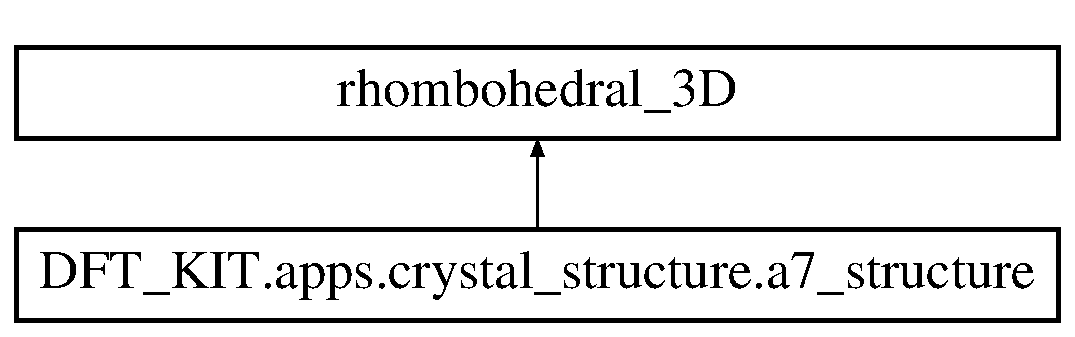
\includegraphics[height=2.000000cm]{class_d_f_t___k_i_t_1_1apps_1_1crystal__structure_1_1a7__structure}
\end{center}
\end{figure}
\subsection*{Public Member Functions}
\begin{DoxyCompactItemize}
\item 
def \hyperlink{class_d_f_t___k_i_t_1_1apps_1_1crystal__structure_1_1a7__structure_a26ee20d73969ab27dcc83e2969ce05ef}{\+\_\+\+\_\+init\+\_\+\+\_\+}
\end{DoxyCompactItemize}


\subsection{Detailed Description}


Definition at line 9 of file crystal\+\_\+structure.\+py.



\subsection{Constructor \& Destructor Documentation}
\hypertarget{class_d_f_t___k_i_t_1_1apps_1_1crystal__structure_1_1a7__structure_a26ee20d73969ab27dcc83e2969ce05ef}{\index{D\+F\+T\+\_\+\+K\+I\+T\+::apps\+::crystal\+\_\+structure\+::a7\+\_\+structure@{D\+F\+T\+\_\+\+K\+I\+T\+::apps\+::crystal\+\_\+structure\+::a7\+\_\+structure}!\+\_\+\+\_\+init\+\_\+\+\_\+@{\+\_\+\+\_\+init\+\_\+\+\_\+}}
\index{\+\_\+\+\_\+init\+\_\+\+\_\+@{\+\_\+\+\_\+init\+\_\+\+\_\+}!D\+F\+T\+\_\+\+K\+I\+T\+::apps\+::crystal\+\_\+structure\+::a7\+\_\+structure@{D\+F\+T\+\_\+\+K\+I\+T\+::apps\+::crystal\+\_\+structure\+::a7\+\_\+structure}}
\subsubsection[{\+\_\+\+\_\+init\+\_\+\+\_\+}]{\setlength{\rightskip}{0pt plus 5cm}def D\+F\+T\+\_\+\+K\+I\+T.\+apps.\+crystal\+\_\+structure.\+a7\+\_\+structure.\+\_\+\+\_\+init\+\_\+\+\_\+ (
\begin{DoxyParamCaption}
\item[{}]{self, }
\item[{}]{element, }
\item[{}]{length\+\_\+unit = {\ttfamily 1.0}, }
\item[{}]{parms}
\end{DoxyParamCaption}
)}}\label{class_d_f_t___k_i_t_1_1apps_1_1crystal__structure_1_1a7__structure_a26ee20d73969ab27dcc83e2969ce05ef}


Definition at line 10 of file crystal\+\_\+structure.\+py.



The documentation for this class was generated from the following file\+:\begin{DoxyCompactItemize}
\item 
apps/\hyperlink{crystal__structure_8py}{crystal\+\_\+structure.\+py}\end{DoxyCompactItemize}

\hypertarget{class_d_f_t___k_i_t_1_1core_1_1atom_1_1atom}{\section{D\+F\+T\+\_\+\+K\+I\+T.\+core.\+atom.\+atom Class Reference}
\label{class_d_f_t___k_i_t_1_1core_1_1atom_1_1atom}\index{D\+F\+T\+\_\+\+K\+I\+T.\+core.\+atom.\+atom@{D\+F\+T\+\_\+\+K\+I\+T.\+core.\+atom.\+atom}}
}
\subsection*{Public Member Functions}
\begin{DoxyCompactItemize}
\item 
def \hyperlink{class_d_f_t___k_i_t_1_1core_1_1atom_1_1atom_a009c3a74d021cdaa211462bfe264e391}{\+\_\+\+\_\+init\+\_\+\+\_\+}
\item 
def \hyperlink{class_d_f_t___k_i_t_1_1core_1_1atom_1_1atom_a8ceaae389e5072b56b412ef183fd252a}{set\+\_\+magmom}
\item 
def \hyperlink{class_d_f_t___k_i_t_1_1core_1_1atom_1_1atom_ac7edf3f236f2f9e63b3ff72200a49458}{get\+\_\+magmom}
\item 
def \hyperlink{class_d_f_t___k_i_t_1_1core_1_1atom_1_1atom_ae43e598eb4fab99c80df3f3228a5687b}{set\+\_\+position}
\item 
def \hyperlink{class_d_f_t___k_i_t_1_1core_1_1atom_1_1atom_a3fd84add462bb189e9fbb08af3ee73e0}{get\+\_\+position}
\item 
def \hyperlink{class_d_f_t___k_i_t_1_1core_1_1atom_1_1atom_ae6d304a50d01a547c245f6704bed631c}{set\+\_\+parms}
\item 
def \hyperlink{class_d_f_t___k_i_t_1_1core_1_1atom_1_1atom_a8bdb87d4538334de54e57ba8ca05a77c}{get\+\_\+parms}
\item 
def \hyperlink{class_d_f_t___k_i_t_1_1core_1_1atom_1_1atom_a37f68a3051eaa205d8cc5dffc689908c}{remove\+\_\+parm}
\end{DoxyCompactItemize}
\subsection*{Public Attributes}
\begin{DoxyCompactItemize}
\item 
\hyperlink{class_d_f_t___k_i_t_1_1core_1_1atom_1_1atom_a816b1396ea4ca88a59a76983227859b6}{element}
\item 
\hyperlink{class_d_f_t___k_i_t_1_1core_1_1atom_1_1atom_aef47619bab2c82e9ed3b3c4faefde38b}{position}
\item 
\hyperlink{class_d_f_t___k_i_t_1_1core_1_1atom_1_1atom_a60468fdb9054f8921592ffd376e5273e}{magmom}
\item 
\hyperlink{class_d_f_t___k_i_t_1_1core_1_1atom_1_1atom_aa864e96171a072d68ca20e3fcd8665dc}{parms}
\end{DoxyCompactItemize}


\subsection{Detailed Description}


Definition at line 10 of file atom.\+py.



\subsection{Constructor \& Destructor Documentation}
\hypertarget{class_d_f_t___k_i_t_1_1core_1_1atom_1_1atom_a009c3a74d021cdaa211462bfe264e391}{\index{D\+F\+T\+\_\+\+K\+I\+T\+::core\+::atom\+::atom@{D\+F\+T\+\_\+\+K\+I\+T\+::core\+::atom\+::atom}!\+\_\+\+\_\+init\+\_\+\+\_\+@{\+\_\+\+\_\+init\+\_\+\+\_\+}}
\index{\+\_\+\+\_\+init\+\_\+\+\_\+@{\+\_\+\+\_\+init\+\_\+\+\_\+}!D\+F\+T\+\_\+\+K\+I\+T\+::core\+::atom\+::atom@{D\+F\+T\+\_\+\+K\+I\+T\+::core\+::atom\+::atom}}
\subsubsection[{\+\_\+\+\_\+init\+\_\+\+\_\+}]{\setlength{\rightskip}{0pt plus 5cm}def D\+F\+T\+\_\+\+K\+I\+T.\+core.\+atom.\+atom.\+\_\+\+\_\+init\+\_\+\+\_\+ (
\begin{DoxyParamCaption}
\item[{}]{self, }
\item[{}]{element, }
\item[{}]{position = {\ttfamily np.array(\mbox{[}0.0,0.0}, }
\item[{}]{parms}
\end{DoxyParamCaption}
)}}\label{class_d_f_t___k_i_t_1_1core_1_1atom_1_1atom_a009c3a74d021cdaa211462bfe264e391}


Definition at line 11 of file atom.\+py.



\subsection{Member Function Documentation}
\hypertarget{class_d_f_t___k_i_t_1_1core_1_1atom_1_1atom_ac7edf3f236f2f9e63b3ff72200a49458}{\index{D\+F\+T\+\_\+\+K\+I\+T\+::core\+::atom\+::atom@{D\+F\+T\+\_\+\+K\+I\+T\+::core\+::atom\+::atom}!get\+\_\+magmom@{get\+\_\+magmom}}
\index{get\+\_\+magmom@{get\+\_\+magmom}!D\+F\+T\+\_\+\+K\+I\+T\+::core\+::atom\+::atom@{D\+F\+T\+\_\+\+K\+I\+T\+::core\+::atom\+::atom}}
\subsubsection[{get\+\_\+magmom}]{\setlength{\rightskip}{0pt plus 5cm}def D\+F\+T\+\_\+\+K\+I\+T.\+core.\+atom.\+atom.\+get\+\_\+magmom (
\begin{DoxyParamCaption}
\item[{}]{self}
\end{DoxyParamCaption}
)}}\label{class_d_f_t___k_i_t_1_1core_1_1atom_1_1atom_ac7edf3f236f2f9e63b3ff72200a49458}


Definition at line 21 of file atom.\+py.

\hypertarget{class_d_f_t___k_i_t_1_1core_1_1atom_1_1atom_a8bdb87d4538334de54e57ba8ca05a77c}{\index{D\+F\+T\+\_\+\+K\+I\+T\+::core\+::atom\+::atom@{D\+F\+T\+\_\+\+K\+I\+T\+::core\+::atom\+::atom}!get\+\_\+parms@{get\+\_\+parms}}
\index{get\+\_\+parms@{get\+\_\+parms}!D\+F\+T\+\_\+\+K\+I\+T\+::core\+::atom\+::atom@{D\+F\+T\+\_\+\+K\+I\+T\+::core\+::atom\+::atom}}
\subsubsection[{get\+\_\+parms}]{\setlength{\rightskip}{0pt plus 5cm}def D\+F\+T\+\_\+\+K\+I\+T.\+core.\+atom.\+atom.\+get\+\_\+parms (
\begin{DoxyParamCaption}
\item[{}]{self, }
\item[{}]{ind\+\_\+parm}
\end{DoxyParamCaption}
)}}\label{class_d_f_t___k_i_t_1_1core_1_1atom_1_1atom_a8bdb87d4538334de54e57ba8ca05a77c}


Definition at line 30 of file atom.\+py.

\hypertarget{class_d_f_t___k_i_t_1_1core_1_1atom_1_1atom_a3fd84add462bb189e9fbb08af3ee73e0}{\index{D\+F\+T\+\_\+\+K\+I\+T\+::core\+::atom\+::atom@{D\+F\+T\+\_\+\+K\+I\+T\+::core\+::atom\+::atom}!get\+\_\+position@{get\+\_\+position}}
\index{get\+\_\+position@{get\+\_\+position}!D\+F\+T\+\_\+\+K\+I\+T\+::core\+::atom\+::atom@{D\+F\+T\+\_\+\+K\+I\+T\+::core\+::atom\+::atom}}
\subsubsection[{get\+\_\+position}]{\setlength{\rightskip}{0pt plus 5cm}def D\+F\+T\+\_\+\+K\+I\+T.\+core.\+atom.\+atom.\+get\+\_\+position (
\begin{DoxyParamCaption}
\item[{}]{self}
\end{DoxyParamCaption}
)}}\label{class_d_f_t___k_i_t_1_1core_1_1atom_1_1atom_a3fd84add462bb189e9fbb08af3ee73e0}


Definition at line 25 of file atom.\+py.

\hypertarget{class_d_f_t___k_i_t_1_1core_1_1atom_1_1atom_a37f68a3051eaa205d8cc5dffc689908c}{\index{D\+F\+T\+\_\+\+K\+I\+T\+::core\+::atom\+::atom@{D\+F\+T\+\_\+\+K\+I\+T\+::core\+::atom\+::atom}!remove\+\_\+parm@{remove\+\_\+parm}}
\index{remove\+\_\+parm@{remove\+\_\+parm}!D\+F\+T\+\_\+\+K\+I\+T\+::core\+::atom\+::atom@{D\+F\+T\+\_\+\+K\+I\+T\+::core\+::atom\+::atom}}
\subsubsection[{remove\+\_\+parm}]{\setlength{\rightskip}{0pt plus 5cm}def D\+F\+T\+\_\+\+K\+I\+T.\+core.\+atom.\+atom.\+remove\+\_\+parm (
\begin{DoxyParamCaption}
\item[{}]{self, }
\item[{}]{ind\+\_\+parm}
\end{DoxyParamCaption}
)}}\label{class_d_f_t___k_i_t_1_1core_1_1atom_1_1atom_a37f68a3051eaa205d8cc5dffc689908c}


Definition at line 32 of file atom.\+py.

\hypertarget{class_d_f_t___k_i_t_1_1core_1_1atom_1_1atom_a8ceaae389e5072b56b412ef183fd252a}{\index{D\+F\+T\+\_\+\+K\+I\+T\+::core\+::atom\+::atom@{D\+F\+T\+\_\+\+K\+I\+T\+::core\+::atom\+::atom}!set\+\_\+magmom@{set\+\_\+magmom}}
\index{set\+\_\+magmom@{set\+\_\+magmom}!D\+F\+T\+\_\+\+K\+I\+T\+::core\+::atom\+::atom@{D\+F\+T\+\_\+\+K\+I\+T\+::core\+::atom\+::atom}}
\subsubsection[{set\+\_\+magmom}]{\setlength{\rightskip}{0pt plus 5cm}def D\+F\+T\+\_\+\+K\+I\+T.\+core.\+atom.\+atom.\+set\+\_\+magmom (
\begin{DoxyParamCaption}
\item[{}]{self, }
\item[{}]{magmom}
\end{DoxyParamCaption}
)}}\label{class_d_f_t___k_i_t_1_1core_1_1atom_1_1atom_a8ceaae389e5072b56b412ef183fd252a}


Definition at line 19 of file atom.\+py.

\hypertarget{class_d_f_t___k_i_t_1_1core_1_1atom_1_1atom_ae6d304a50d01a547c245f6704bed631c}{\index{D\+F\+T\+\_\+\+K\+I\+T\+::core\+::atom\+::atom@{D\+F\+T\+\_\+\+K\+I\+T\+::core\+::atom\+::atom}!set\+\_\+parms@{set\+\_\+parms}}
\index{set\+\_\+parms@{set\+\_\+parms}!D\+F\+T\+\_\+\+K\+I\+T\+::core\+::atom\+::atom@{D\+F\+T\+\_\+\+K\+I\+T\+::core\+::atom\+::atom}}
\subsubsection[{set\+\_\+parms}]{\setlength{\rightskip}{0pt plus 5cm}def D\+F\+T\+\_\+\+K\+I\+T.\+core.\+atom.\+atom.\+set\+\_\+parms (
\begin{DoxyParamCaption}
\item[{}]{self, }
\item[{}]{parms}
\end{DoxyParamCaption}
)}}\label{class_d_f_t___k_i_t_1_1core_1_1atom_1_1atom_ae6d304a50d01a547c245f6704bed631c}


Definition at line 27 of file atom.\+py.

\hypertarget{class_d_f_t___k_i_t_1_1core_1_1atom_1_1atom_ae43e598eb4fab99c80df3f3228a5687b}{\index{D\+F\+T\+\_\+\+K\+I\+T\+::core\+::atom\+::atom@{D\+F\+T\+\_\+\+K\+I\+T\+::core\+::atom\+::atom}!set\+\_\+position@{set\+\_\+position}}
\index{set\+\_\+position@{set\+\_\+position}!D\+F\+T\+\_\+\+K\+I\+T\+::core\+::atom\+::atom@{D\+F\+T\+\_\+\+K\+I\+T\+::core\+::atom\+::atom}}
\subsubsection[{set\+\_\+position}]{\setlength{\rightskip}{0pt plus 5cm}def D\+F\+T\+\_\+\+K\+I\+T.\+core.\+atom.\+atom.\+set\+\_\+position (
\begin{DoxyParamCaption}
\item[{}]{self, }
\item[{}]{pos\+\_\+}
\end{DoxyParamCaption}
)}}\label{class_d_f_t___k_i_t_1_1core_1_1atom_1_1atom_ae43e598eb4fab99c80df3f3228a5687b}


Definition at line 23 of file atom.\+py.



\subsection{Member Data Documentation}
\hypertarget{class_d_f_t___k_i_t_1_1core_1_1atom_1_1atom_a816b1396ea4ca88a59a76983227859b6}{\index{D\+F\+T\+\_\+\+K\+I\+T\+::core\+::atom\+::atom@{D\+F\+T\+\_\+\+K\+I\+T\+::core\+::atom\+::atom}!element@{element}}
\index{element@{element}!D\+F\+T\+\_\+\+K\+I\+T\+::core\+::atom\+::atom@{D\+F\+T\+\_\+\+K\+I\+T\+::core\+::atom\+::atom}}
\subsubsection[{element}]{\setlength{\rightskip}{0pt plus 5cm}D\+F\+T\+\_\+\+K\+I\+T.\+core.\+atom.\+atom.\+element}}\label{class_d_f_t___k_i_t_1_1core_1_1atom_1_1atom_a816b1396ea4ca88a59a76983227859b6}


Definition at line 12 of file atom.\+py.

\hypertarget{class_d_f_t___k_i_t_1_1core_1_1atom_1_1atom_a60468fdb9054f8921592ffd376e5273e}{\index{D\+F\+T\+\_\+\+K\+I\+T\+::core\+::atom\+::atom@{D\+F\+T\+\_\+\+K\+I\+T\+::core\+::atom\+::atom}!magmom@{magmom}}
\index{magmom@{magmom}!D\+F\+T\+\_\+\+K\+I\+T\+::core\+::atom\+::atom@{D\+F\+T\+\_\+\+K\+I\+T\+::core\+::atom\+::atom}}
\subsubsection[{magmom}]{\setlength{\rightskip}{0pt plus 5cm}D\+F\+T\+\_\+\+K\+I\+T.\+core.\+atom.\+atom.\+magmom}}\label{class_d_f_t___k_i_t_1_1core_1_1atom_1_1atom_a60468fdb9054f8921592ffd376e5273e}


Definition at line 14 of file atom.\+py.

\hypertarget{class_d_f_t___k_i_t_1_1core_1_1atom_1_1atom_aa864e96171a072d68ca20e3fcd8665dc}{\index{D\+F\+T\+\_\+\+K\+I\+T\+::core\+::atom\+::atom@{D\+F\+T\+\_\+\+K\+I\+T\+::core\+::atom\+::atom}!parms@{parms}}
\index{parms@{parms}!D\+F\+T\+\_\+\+K\+I\+T\+::core\+::atom\+::atom@{D\+F\+T\+\_\+\+K\+I\+T\+::core\+::atom\+::atom}}
\subsubsection[{parms}]{\setlength{\rightskip}{0pt plus 5cm}D\+F\+T\+\_\+\+K\+I\+T.\+core.\+atom.\+atom.\+parms}}\label{class_d_f_t___k_i_t_1_1core_1_1atom_1_1atom_aa864e96171a072d68ca20e3fcd8665dc}


Definition at line 15 of file atom.\+py.

\hypertarget{class_d_f_t___k_i_t_1_1core_1_1atom_1_1atom_aef47619bab2c82e9ed3b3c4faefde38b}{\index{D\+F\+T\+\_\+\+K\+I\+T\+::core\+::atom\+::atom@{D\+F\+T\+\_\+\+K\+I\+T\+::core\+::atom\+::atom}!position@{position}}
\index{position@{position}!D\+F\+T\+\_\+\+K\+I\+T\+::core\+::atom\+::atom@{D\+F\+T\+\_\+\+K\+I\+T\+::core\+::atom\+::atom}}
\subsubsection[{position}]{\setlength{\rightskip}{0pt plus 5cm}D\+F\+T\+\_\+\+K\+I\+T.\+core.\+atom.\+atom.\+position}}\label{class_d_f_t___k_i_t_1_1core_1_1atom_1_1atom_aef47619bab2c82e9ed3b3c4faefde38b}


Definition at line 13 of file atom.\+py.



The documentation for this class was generated from the following file\+:\begin{DoxyCompactItemize}
\item 
core/\hyperlink{atom_8py}{atom.\+py}\end{DoxyCompactItemize}

\hypertarget{class_d_f_t___k_i_t_1_1core_1_1crystal__3_d_1_1bcc__3_d}{\section{D\+F\+T\+\_\+\+K\+I\+T.\+core.\+crystal\+\_\+3\+D.\+bcc\+\_\+3\+D Class Reference}
\label{class_d_f_t___k_i_t_1_1core_1_1crystal__3_d_1_1bcc__3_d}\index{D\+F\+T\+\_\+\+K\+I\+T.\+core.\+crystal\+\_\+3\+D.\+bcc\+\_\+3\+D@{D\+F\+T\+\_\+\+K\+I\+T.\+core.\+crystal\+\_\+3\+D.\+bcc\+\_\+3\+D}}
}
Inheritance diagram for D\+F\+T\+\_\+\+K\+I\+T.\+core.\+crystal\+\_\+3\+D.\+bcc\+\_\+3\+D\+:\begin{figure}[H]
\begin{center}
\leavevmode
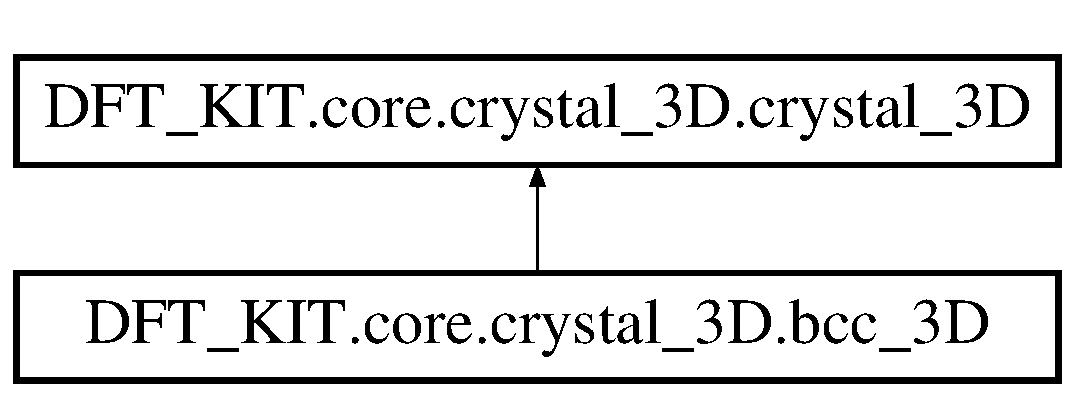
\includegraphics[height=2.000000cm]{class_d_f_t___k_i_t_1_1core_1_1crystal__3_d_1_1bcc__3_d}
\end{center}
\end{figure}
\subsection*{Public Member Functions}
\begin{DoxyCompactItemize}
\item 
def \hyperlink{class_d_f_t___k_i_t_1_1core_1_1crystal__3_d_1_1bcc__3_d_a909776a325e8a2391f658c4dbed6d14f}{\+\_\+\+\_\+init\+\_\+\+\_\+}
\item 
def \hyperlink{class_d_f_t___k_i_t_1_1core_1_1crystal__3_d_1_1bcc__3_d_aeb82880d1d70d1be856ceb6926c191cb}{set\+\_\+lattice}
\item 
def \hyperlink{class_d_f_t___k_i_t_1_1core_1_1crystal__3_d_1_1bcc__3_d_a37169d59118daa78f4f41aefd25a104d}{define\+\_\+klabels}
\end{DoxyCompactItemize}
\subsection*{Additional Inherited Members}


\subsection{Detailed Description}


Definition at line 170 of file crystal\+\_\+3\+D.\+py.



\subsection{Constructor \& Destructor Documentation}
\hypertarget{class_d_f_t___k_i_t_1_1core_1_1crystal__3_d_1_1bcc__3_d_a909776a325e8a2391f658c4dbed6d14f}{\index{D\+F\+T\+\_\+\+K\+I\+T\+::core\+::crystal\+\_\+3\+D\+::bcc\+\_\+3\+D@{D\+F\+T\+\_\+\+K\+I\+T\+::core\+::crystal\+\_\+3\+D\+::bcc\+\_\+3\+D}!\+\_\+\+\_\+init\+\_\+\+\_\+@{\+\_\+\+\_\+init\+\_\+\+\_\+}}
\index{\+\_\+\+\_\+init\+\_\+\+\_\+@{\+\_\+\+\_\+init\+\_\+\+\_\+}!D\+F\+T\+\_\+\+K\+I\+T\+::core\+::crystal\+\_\+3\+D\+::bcc\+\_\+3\+D@{D\+F\+T\+\_\+\+K\+I\+T\+::core\+::crystal\+\_\+3\+D\+::bcc\+\_\+3\+D}}
\subsubsection[{\+\_\+\+\_\+init\+\_\+\+\_\+}]{\setlength{\rightskip}{0pt plus 5cm}def D\+F\+T\+\_\+\+K\+I\+T.\+core.\+crystal\+\_\+3\+D.\+bcc\+\_\+3\+D.\+\_\+\+\_\+init\+\_\+\+\_\+ (
\begin{DoxyParamCaption}
\item[{}]{self, }
\item[{}]{bcc\+\_\+length, }
\item[{}]{length\+\_\+unit = {\ttfamily 1.0}}
\end{DoxyParamCaption}
)}}\label{class_d_f_t___k_i_t_1_1core_1_1crystal__3_d_1_1bcc__3_d_a909776a325e8a2391f658c4dbed6d14f}


Definition at line 171 of file crystal\+\_\+3\+D.\+py.



\subsection{Member Function Documentation}
\hypertarget{class_d_f_t___k_i_t_1_1core_1_1crystal__3_d_1_1bcc__3_d_a37169d59118daa78f4f41aefd25a104d}{\index{D\+F\+T\+\_\+\+K\+I\+T\+::core\+::crystal\+\_\+3\+D\+::bcc\+\_\+3\+D@{D\+F\+T\+\_\+\+K\+I\+T\+::core\+::crystal\+\_\+3\+D\+::bcc\+\_\+3\+D}!define\+\_\+klabels@{define\+\_\+klabels}}
\index{define\+\_\+klabels@{define\+\_\+klabels}!D\+F\+T\+\_\+\+K\+I\+T\+::core\+::crystal\+\_\+3\+D\+::bcc\+\_\+3\+D@{D\+F\+T\+\_\+\+K\+I\+T\+::core\+::crystal\+\_\+3\+D\+::bcc\+\_\+3\+D}}
\subsubsection[{define\+\_\+klabels}]{\setlength{\rightskip}{0pt plus 5cm}def D\+F\+T\+\_\+\+K\+I\+T.\+core.\+crystal\+\_\+3\+D.\+bcc\+\_\+3\+D.\+define\+\_\+klabels (
\begin{DoxyParamCaption}
\item[{}]{self}
\end{DoxyParamCaption}
)}}\label{class_d_f_t___k_i_t_1_1core_1_1crystal__3_d_1_1bcc__3_d_a37169d59118daa78f4f41aefd25a104d}


Definition at line 183 of file crystal\+\_\+3\+D.\+py.

\hypertarget{class_d_f_t___k_i_t_1_1core_1_1crystal__3_d_1_1bcc__3_d_aeb82880d1d70d1be856ceb6926c191cb}{\index{D\+F\+T\+\_\+\+K\+I\+T\+::core\+::crystal\+\_\+3\+D\+::bcc\+\_\+3\+D@{D\+F\+T\+\_\+\+K\+I\+T\+::core\+::crystal\+\_\+3\+D\+::bcc\+\_\+3\+D}!set\+\_\+lattice@{set\+\_\+lattice}}
\index{set\+\_\+lattice@{set\+\_\+lattice}!D\+F\+T\+\_\+\+K\+I\+T\+::core\+::crystal\+\_\+3\+D\+::bcc\+\_\+3\+D@{D\+F\+T\+\_\+\+K\+I\+T\+::core\+::crystal\+\_\+3\+D\+::bcc\+\_\+3\+D}}
\subsubsection[{set\+\_\+lattice}]{\setlength{\rightskip}{0pt plus 5cm}def D\+F\+T\+\_\+\+K\+I\+T.\+core.\+crystal\+\_\+3\+D.\+bcc\+\_\+3\+D.\+set\+\_\+lattice (
\begin{DoxyParamCaption}
\item[{}]{self, }
\item[{}]{bcc\+\_\+length}
\end{DoxyParamCaption}
)}}\label{class_d_f_t___k_i_t_1_1core_1_1crystal__3_d_1_1bcc__3_d_aeb82880d1d70d1be856ceb6926c191cb}


Definition at line 176 of file crystal\+\_\+3\+D.\+py.



The documentation for this class was generated from the following file\+:\begin{DoxyCompactItemize}
\item 
core/\hyperlink{crystal__3_d_8py}{crystal\+\_\+3\+D.\+py}\end{DoxyCompactItemize}

\hypertarget{class_d_f_t___k_i_t_1_1apps_1_1crystal__structure_1_1body__center}{\section{D\+F\+T\+\_\+\+K\+I\+T.\+apps.\+crystal\+\_\+structure.\+body\+\_\+center Class Reference}
\label{class_d_f_t___k_i_t_1_1apps_1_1crystal__structure_1_1body__center}\index{D\+F\+T\+\_\+\+K\+I\+T.\+apps.\+crystal\+\_\+structure.\+body\+\_\+center@{D\+F\+T\+\_\+\+K\+I\+T.\+apps.\+crystal\+\_\+structure.\+body\+\_\+center}}
}
Inheritance diagram for D\+F\+T\+\_\+\+K\+I\+T.\+apps.\+crystal\+\_\+structure.\+body\+\_\+center\+:\begin{figure}[H]
\begin{center}
\leavevmode
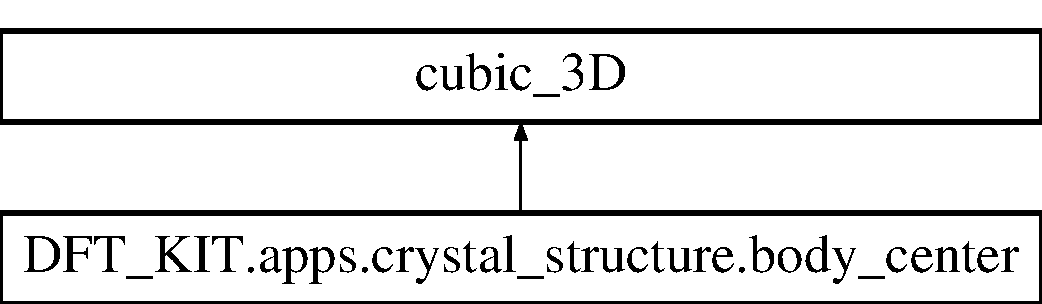
\includegraphics[height=2.000000cm]{class_d_f_t___k_i_t_1_1apps_1_1crystal__structure_1_1body__center}
\end{center}
\end{figure}
\subsection*{Public Member Functions}
\begin{DoxyCompactItemize}
\item 
def \hyperlink{class_d_f_t___k_i_t_1_1apps_1_1crystal__structure_1_1body__center_aace7b55a229068943fc34a22f89f8892}{\+\_\+\+\_\+init\+\_\+\+\_\+}
\end{DoxyCompactItemize}


\subsection{Detailed Description}


Definition at line 60 of file crystal\+\_\+structure.\+py.



\subsection{Constructor \& Destructor Documentation}
\hypertarget{class_d_f_t___k_i_t_1_1apps_1_1crystal__structure_1_1body__center_aace7b55a229068943fc34a22f89f8892}{\index{D\+F\+T\+\_\+\+K\+I\+T\+::apps\+::crystal\+\_\+structure\+::body\+\_\+center@{D\+F\+T\+\_\+\+K\+I\+T\+::apps\+::crystal\+\_\+structure\+::body\+\_\+center}!\+\_\+\+\_\+init\+\_\+\+\_\+@{\+\_\+\+\_\+init\+\_\+\+\_\+}}
\index{\+\_\+\+\_\+init\+\_\+\+\_\+@{\+\_\+\+\_\+init\+\_\+\+\_\+}!D\+F\+T\+\_\+\+K\+I\+T\+::apps\+::crystal\+\_\+structure\+::body\+\_\+center@{D\+F\+T\+\_\+\+K\+I\+T\+::apps\+::crystal\+\_\+structure\+::body\+\_\+center}}
\subsubsection[{\+\_\+\+\_\+init\+\_\+\+\_\+}]{\setlength{\rightskip}{0pt plus 5cm}def D\+F\+T\+\_\+\+K\+I\+T.\+apps.\+crystal\+\_\+structure.\+body\+\_\+center.\+\_\+\+\_\+init\+\_\+\+\_\+ (
\begin{DoxyParamCaption}
\item[{}]{self, }
\item[{}]{cubic\+\_\+length, }
\item[{}]{length\+\_\+unit = {\ttfamily 1.0}}
\end{DoxyParamCaption}
)}}\label{class_d_f_t___k_i_t_1_1apps_1_1crystal__structure_1_1body__center_aace7b55a229068943fc34a22f89f8892}


Definition at line 61 of file crystal\+\_\+structure.\+py.



The documentation for this class was generated from the following file\+:\begin{DoxyCompactItemize}
\item 
apps/\hyperlink{crystal__structure_8py}{crystal\+\_\+structure.\+py}\end{DoxyCompactItemize}

\hypertarget{class_d_f_t___k_i_t_1_1core_1_1calculator_1_1calculator}{\section{D\+F\+T\+\_\+\+K\+I\+T.\+core.\+calculator.\+calculator Class Reference}
\label{class_d_f_t___k_i_t_1_1core_1_1calculator_1_1calculator}\index{D\+F\+T\+\_\+\+K\+I\+T.\+core.\+calculator.\+calculator@{D\+F\+T\+\_\+\+K\+I\+T.\+core.\+calculator.\+calculator}}
}
\subsection*{Public Member Functions}
\begin{DoxyCompactItemize}
\item 
def \hyperlink{class_d_f_t___k_i_t_1_1core_1_1calculator_1_1calculator_a313297ecdb7f0ad50e2fa1d228cf783a}{\+\_\+\+\_\+init\+\_\+\+\_\+}
\item 
def \hyperlink{class_d_f_t___k_i_t_1_1core_1_1calculator_1_1calculator_a4302c90c91ad7492477f186623a397ae}{run\+\_\+calculation}
\item 
def \hyperlink{class_d_f_t___k_i_t_1_1core_1_1calculator_1_1calculator_afe281732adf9c5d00ee24ca42d4bcdfb}{get\+\_\+maindir}
\item 
def \hyperlink{class_d_f_t___k_i_t_1_1core_1_1calculator_1_1calculator_a6a4bba344e3d0bb74114dba596961c00}{set\+\_\+output\+\_\+dir}
\item 
def \hyperlink{class_d_f_t___k_i_t_1_1core_1_1calculator_1_1calculator_aeec37a45539b01186913578d48d10050}{get\+\_\+output\+\_\+dir}
\item 
def \hyperlink{class_d_f_t___k_i_t_1_1core_1_1calculator_1_1calculator_af6f9312c2f7f28813af872338e53ade4}{set\+\_\+parm}
\item 
def \hyperlink{class_d_f_t___k_i_t_1_1core_1_1calculator_1_1calculator_a65adbeb005dc8329e2b0e97a94d5d940}{get\+\_\+parm}
\item 
def \hyperlink{class_d_f_t___k_i_t_1_1core_1_1calculator_1_1calculator_a09cef9e96371423beaad7f0669e95604}{load\+\_\+parm}
\item 
def \hyperlink{class_d_f_t___k_i_t_1_1core_1_1calculator_1_1calculator_acc7d0eb2f9e4ce3492689c6e47f82e1b}{remove\+\_\+parm}
\item 
def \hyperlink{class_d_f_t___k_i_t_1_1core_1_1calculator_1_1calculator_a7ca6ca9b626a34bc52b5e5988f5f0399}{get\+\_\+crystal}
\item 
def \hyperlink{class_d_f_t___k_i_t_1_1core_1_1calculator_1_1calculator_ae8fab5d1aacf567c099250097ed7b489}{set\+\_\+crystal}
\item 
def \hyperlink{class_d_f_t___k_i_t_1_1core_1_1calculator_1_1calculator_aebc75e85c7b1e21c6d75aee30e6a8e18}{set\+\_\+postprocess}
\item 
def \hyperlink{class_d_f_t___k_i_t_1_1core_1_1calculator_1_1calculator_a6ff775d23aacefd9e577ea1e21a822cc}{clean}
\item 
def \hyperlink{class_d_f_t___k_i_t_1_1core_1_1calculator_1_1calculator_ae521ab992ae87366896752575005836e}{reset\+\_\+simulation\+\_\+data}
\end{DoxyCompactItemize}
\subsection*{Public Attributes}
\begin{DoxyCompactItemize}
\item 
\hyperlink{class_d_f_t___k_i_t_1_1core_1_1calculator_1_1calculator_af9be1ce4c811d9ff7146973115d9e254}{output\+\_\+dir}
\item 
\hyperlink{class_d_f_t___k_i_t_1_1core_1_1calculator_1_1calculator_a5e80e925c9765c6d4763fce2d531bfce}{crystal}
\item 
\hyperlink{class_d_f_t___k_i_t_1_1core_1_1calculator_1_1calculator_a6dab8a54556ccbfbdb4f6e6ae9b7e5aa}{kgrid}
\item 
\hyperlink{class_d_f_t___k_i_t_1_1core_1_1calculator_1_1calculator_a19b88dafd31c5ed3dc5fa31922716d74}{parms}
\item 
\hyperlink{class_d_f_t___k_i_t_1_1core_1_1calculator_1_1calculator_a8ae7016b72ab4e047242b2aeb3e5ce68}{postprocess}
\item 
\hyperlink{class_d_f_t___k_i_t_1_1core_1_1calculator_1_1calculator_a4724f290121a7f108b0b00a790ead330}{dft\+\_\+job}
\item 
\hyperlink{class_d_f_t___k_i_t_1_1core_1_1calculator_1_1calculator_aa16b2c67c6adf6c612f76b485292d8a8}{pre\+\_\+commands}
\item 
\hyperlink{class_d_f_t___k_i_t_1_1core_1_1calculator_1_1calculator_a0b83a4e589b749c56e54c5d42e0049d5}{post\+\_\+commands}
\item 
\hyperlink{class_d_f_t___k_i_t_1_1core_1_1calculator_1_1calculator_a52df0fa66d2e031689fa0a1ea9366fe9}{output}
\end{DoxyCompactItemize}


\subsection{Detailed Description}


Definition at line 12 of file calculator.\+py.



\subsection{Constructor \& Destructor Documentation}
\hypertarget{class_d_f_t___k_i_t_1_1core_1_1calculator_1_1calculator_a313297ecdb7f0ad50e2fa1d228cf783a}{\index{D\+F\+T\+\_\+\+K\+I\+T\+::core\+::calculator\+::calculator@{D\+F\+T\+\_\+\+K\+I\+T\+::core\+::calculator\+::calculator}!\+\_\+\+\_\+init\+\_\+\+\_\+@{\+\_\+\+\_\+init\+\_\+\+\_\+}}
\index{\+\_\+\+\_\+init\+\_\+\+\_\+@{\+\_\+\+\_\+init\+\_\+\+\_\+}!D\+F\+T\+\_\+\+K\+I\+T\+::core\+::calculator\+::calculator@{D\+F\+T\+\_\+\+K\+I\+T\+::core\+::calculator\+::calculator}}
\subsubsection[{\+\_\+\+\_\+init\+\_\+\+\_\+}]{\setlength{\rightskip}{0pt plus 5cm}def D\+F\+T\+\_\+\+K\+I\+T.\+core.\+calculator.\+calculator.\+\_\+\+\_\+init\+\_\+\+\_\+ (
\begin{DoxyParamCaption}
\item[{}]{self, }
\item[{}]{postprocess, }
\item[{}]{dft\+\_\+job, }
\item[{}]{crystal, }
\item[{}]{kgrid, }
\item[{}]{parms}
\end{DoxyParamCaption}
)}}\label{class_d_f_t___k_i_t_1_1core_1_1calculator_1_1calculator_a313297ecdb7f0ad50e2fa1d228cf783a}


Definition at line 13 of file calculator.\+py.



\subsection{Member Function Documentation}
\hypertarget{class_d_f_t___k_i_t_1_1core_1_1calculator_1_1calculator_a6ff775d23aacefd9e577ea1e21a822cc}{\index{D\+F\+T\+\_\+\+K\+I\+T\+::core\+::calculator\+::calculator@{D\+F\+T\+\_\+\+K\+I\+T\+::core\+::calculator\+::calculator}!clean@{clean}}
\index{clean@{clean}!D\+F\+T\+\_\+\+K\+I\+T\+::core\+::calculator\+::calculator@{D\+F\+T\+\_\+\+K\+I\+T\+::core\+::calculator\+::calculator}}
\subsubsection[{clean}]{\setlength{\rightskip}{0pt plus 5cm}def D\+F\+T\+\_\+\+K\+I\+T.\+core.\+calculator.\+calculator.\+clean (
\begin{DoxyParamCaption}
\item[{}]{self}
\end{DoxyParamCaption}
)}}\label{class_d_f_t___k_i_t_1_1core_1_1calculator_1_1calculator_a6ff775d23aacefd9e577ea1e21a822cc}


Definition at line 75 of file calculator.\+py.

\hypertarget{class_d_f_t___k_i_t_1_1core_1_1calculator_1_1calculator_a7ca6ca9b626a34bc52b5e5988f5f0399}{\index{D\+F\+T\+\_\+\+K\+I\+T\+::core\+::calculator\+::calculator@{D\+F\+T\+\_\+\+K\+I\+T\+::core\+::calculator\+::calculator}!get\+\_\+crystal@{get\+\_\+crystal}}
\index{get\+\_\+crystal@{get\+\_\+crystal}!D\+F\+T\+\_\+\+K\+I\+T\+::core\+::calculator\+::calculator@{D\+F\+T\+\_\+\+K\+I\+T\+::core\+::calculator\+::calculator}}
\subsubsection[{get\+\_\+crystal}]{\setlength{\rightskip}{0pt plus 5cm}def D\+F\+T\+\_\+\+K\+I\+T.\+core.\+calculator.\+calculator.\+get\+\_\+crystal (
\begin{DoxyParamCaption}
\item[{}]{self}
\end{DoxyParamCaption}
)}}\label{class_d_f_t___k_i_t_1_1core_1_1calculator_1_1calculator_a7ca6ca9b626a34bc52b5e5988f5f0399}


Definition at line 68 of file calculator.\+py.

\hypertarget{class_d_f_t___k_i_t_1_1core_1_1calculator_1_1calculator_afe281732adf9c5d00ee24ca42d4bcdfb}{\index{D\+F\+T\+\_\+\+K\+I\+T\+::core\+::calculator\+::calculator@{D\+F\+T\+\_\+\+K\+I\+T\+::core\+::calculator\+::calculator}!get\+\_\+maindir@{get\+\_\+maindir}}
\index{get\+\_\+maindir@{get\+\_\+maindir}!D\+F\+T\+\_\+\+K\+I\+T\+::core\+::calculator\+::calculator@{D\+F\+T\+\_\+\+K\+I\+T\+::core\+::calculator\+::calculator}}
\subsubsection[{get\+\_\+maindir}]{\setlength{\rightskip}{0pt plus 5cm}def D\+F\+T\+\_\+\+K\+I\+T.\+core.\+calculator.\+calculator.\+get\+\_\+maindir (
\begin{DoxyParamCaption}
\item[{}]{self}
\end{DoxyParamCaption}
)}}\label{class_d_f_t___k_i_t_1_1core_1_1calculator_1_1calculator_afe281732adf9c5d00ee24ca42d4bcdfb}


Definition at line 47 of file calculator.\+py.

\hypertarget{class_d_f_t___k_i_t_1_1core_1_1calculator_1_1calculator_aeec37a45539b01186913578d48d10050}{\index{D\+F\+T\+\_\+\+K\+I\+T\+::core\+::calculator\+::calculator@{D\+F\+T\+\_\+\+K\+I\+T\+::core\+::calculator\+::calculator}!get\+\_\+output\+\_\+dir@{get\+\_\+output\+\_\+dir}}
\index{get\+\_\+output\+\_\+dir@{get\+\_\+output\+\_\+dir}!D\+F\+T\+\_\+\+K\+I\+T\+::core\+::calculator\+::calculator@{D\+F\+T\+\_\+\+K\+I\+T\+::core\+::calculator\+::calculator}}
\subsubsection[{get\+\_\+output\+\_\+dir}]{\setlength{\rightskip}{0pt plus 5cm}def D\+F\+T\+\_\+\+K\+I\+T.\+core.\+calculator.\+calculator.\+get\+\_\+output\+\_\+dir (
\begin{DoxyParamCaption}
\item[{}]{self}
\end{DoxyParamCaption}
)}}\label{class_d_f_t___k_i_t_1_1core_1_1calculator_1_1calculator_aeec37a45539b01186913578d48d10050}


Definition at line 52 of file calculator.\+py.

\hypertarget{class_d_f_t___k_i_t_1_1core_1_1calculator_1_1calculator_a65adbeb005dc8329e2b0e97a94d5d940}{\index{D\+F\+T\+\_\+\+K\+I\+T\+::core\+::calculator\+::calculator@{D\+F\+T\+\_\+\+K\+I\+T\+::core\+::calculator\+::calculator}!get\+\_\+parm@{get\+\_\+parm}}
\index{get\+\_\+parm@{get\+\_\+parm}!D\+F\+T\+\_\+\+K\+I\+T\+::core\+::calculator\+::calculator@{D\+F\+T\+\_\+\+K\+I\+T\+::core\+::calculator\+::calculator}}
\subsubsection[{get\+\_\+parm}]{\setlength{\rightskip}{0pt plus 5cm}def D\+F\+T\+\_\+\+K\+I\+T.\+core.\+calculator.\+calculator.\+get\+\_\+parm (
\begin{DoxyParamCaption}
\item[{}]{self, }
\item[{}]{ind\+\_\+key}
\end{DoxyParamCaption}
)}}\label{class_d_f_t___k_i_t_1_1core_1_1calculator_1_1calculator_a65adbeb005dc8329e2b0e97a94d5d940}


Definition at line 56 of file calculator.\+py.

\hypertarget{class_d_f_t___k_i_t_1_1core_1_1calculator_1_1calculator_a09cef9e96371423beaad7f0669e95604}{\index{D\+F\+T\+\_\+\+K\+I\+T\+::core\+::calculator\+::calculator@{D\+F\+T\+\_\+\+K\+I\+T\+::core\+::calculator\+::calculator}!load\+\_\+parm@{load\+\_\+parm}}
\index{load\+\_\+parm@{load\+\_\+parm}!D\+F\+T\+\_\+\+K\+I\+T\+::core\+::calculator\+::calculator@{D\+F\+T\+\_\+\+K\+I\+T\+::core\+::calculator\+::calculator}}
\subsubsection[{load\+\_\+parm}]{\setlength{\rightskip}{0pt plus 5cm}def D\+F\+T\+\_\+\+K\+I\+T.\+core.\+calculator.\+calculator.\+load\+\_\+parm (
\begin{DoxyParamCaption}
\item[{}]{self, }
\item[{}]{cleanup, }
\item[{}]{new\+\_\+parm}
\end{DoxyParamCaption}
)}}\label{class_d_f_t___k_i_t_1_1core_1_1calculator_1_1calculator_a09cef9e96371423beaad7f0669e95604}


Definition at line 58 of file calculator.\+py.

\hypertarget{class_d_f_t___k_i_t_1_1core_1_1calculator_1_1calculator_acc7d0eb2f9e4ce3492689c6e47f82e1b}{\index{D\+F\+T\+\_\+\+K\+I\+T\+::core\+::calculator\+::calculator@{D\+F\+T\+\_\+\+K\+I\+T\+::core\+::calculator\+::calculator}!remove\+\_\+parm@{remove\+\_\+parm}}
\index{remove\+\_\+parm@{remove\+\_\+parm}!D\+F\+T\+\_\+\+K\+I\+T\+::core\+::calculator\+::calculator@{D\+F\+T\+\_\+\+K\+I\+T\+::core\+::calculator\+::calculator}}
\subsubsection[{remove\+\_\+parm}]{\setlength{\rightskip}{0pt plus 5cm}def D\+F\+T\+\_\+\+K\+I\+T.\+core.\+calculator.\+calculator.\+remove\+\_\+parm (
\begin{DoxyParamCaption}
\item[{}]{self, }
\item[{}]{ind\+\_\+key}
\end{DoxyParamCaption}
)}}\label{class_d_f_t___k_i_t_1_1core_1_1calculator_1_1calculator_acc7d0eb2f9e4ce3492689c6e47f82e1b}


Definition at line 65 of file calculator.\+py.

\hypertarget{class_d_f_t___k_i_t_1_1core_1_1calculator_1_1calculator_ae521ab992ae87366896752575005836e}{\index{D\+F\+T\+\_\+\+K\+I\+T\+::core\+::calculator\+::calculator@{D\+F\+T\+\_\+\+K\+I\+T\+::core\+::calculator\+::calculator}!reset\+\_\+simulation\+\_\+data@{reset\+\_\+simulation\+\_\+data}}
\index{reset\+\_\+simulation\+\_\+data@{reset\+\_\+simulation\+\_\+data}!D\+F\+T\+\_\+\+K\+I\+T\+::core\+::calculator\+::calculator@{D\+F\+T\+\_\+\+K\+I\+T\+::core\+::calculator\+::calculator}}
\subsubsection[{reset\+\_\+simulation\+\_\+data}]{\setlength{\rightskip}{0pt plus 5cm}def D\+F\+T\+\_\+\+K\+I\+T.\+core.\+calculator.\+calculator.\+reset\+\_\+simulation\+\_\+data (
\begin{DoxyParamCaption}
\item[{}]{self}
\end{DoxyParamCaption}
)}}\label{class_d_f_t___k_i_t_1_1core_1_1calculator_1_1calculator_ae521ab992ae87366896752575005836e}


Definition at line 78 of file calculator.\+py.

\hypertarget{class_d_f_t___k_i_t_1_1core_1_1calculator_1_1calculator_a4302c90c91ad7492477f186623a397ae}{\index{D\+F\+T\+\_\+\+K\+I\+T\+::core\+::calculator\+::calculator@{D\+F\+T\+\_\+\+K\+I\+T\+::core\+::calculator\+::calculator}!run\+\_\+calculation@{run\+\_\+calculation}}
\index{run\+\_\+calculation@{run\+\_\+calculation}!D\+F\+T\+\_\+\+K\+I\+T\+::core\+::calculator\+::calculator@{D\+F\+T\+\_\+\+K\+I\+T\+::core\+::calculator\+::calculator}}
\subsubsection[{run\+\_\+calculation}]{\setlength{\rightskip}{0pt plus 5cm}def D\+F\+T\+\_\+\+K\+I\+T.\+core.\+calculator.\+calculator.\+run\+\_\+calculation (
\begin{DoxyParamCaption}
\item[{}]{self}
\end{DoxyParamCaption}
)}}\label{class_d_f_t___k_i_t_1_1core_1_1calculator_1_1calculator_a4302c90c91ad7492477f186623a397ae}


Definition at line 32 of file calculator.\+py.

\hypertarget{class_d_f_t___k_i_t_1_1core_1_1calculator_1_1calculator_ae8fab5d1aacf567c099250097ed7b489}{\index{D\+F\+T\+\_\+\+K\+I\+T\+::core\+::calculator\+::calculator@{D\+F\+T\+\_\+\+K\+I\+T\+::core\+::calculator\+::calculator}!set\+\_\+crystal@{set\+\_\+crystal}}
\index{set\+\_\+crystal@{set\+\_\+crystal}!D\+F\+T\+\_\+\+K\+I\+T\+::core\+::calculator\+::calculator@{D\+F\+T\+\_\+\+K\+I\+T\+::core\+::calculator\+::calculator}}
\subsubsection[{set\+\_\+crystal}]{\setlength{\rightskip}{0pt plus 5cm}def D\+F\+T\+\_\+\+K\+I\+T.\+core.\+calculator.\+calculator.\+set\+\_\+crystal (
\begin{DoxyParamCaption}
\item[{}]{self, }
\item[{}]{crystal}
\end{DoxyParamCaption}
)}}\label{class_d_f_t___k_i_t_1_1core_1_1calculator_1_1calculator_ae8fab5d1aacf567c099250097ed7b489}


Definition at line 70 of file calculator.\+py.

\hypertarget{class_d_f_t___k_i_t_1_1core_1_1calculator_1_1calculator_a6a4bba344e3d0bb74114dba596961c00}{\index{D\+F\+T\+\_\+\+K\+I\+T\+::core\+::calculator\+::calculator@{D\+F\+T\+\_\+\+K\+I\+T\+::core\+::calculator\+::calculator}!set\+\_\+output\+\_\+dir@{set\+\_\+output\+\_\+dir}}
\index{set\+\_\+output\+\_\+dir@{set\+\_\+output\+\_\+dir}!D\+F\+T\+\_\+\+K\+I\+T\+::core\+::calculator\+::calculator@{D\+F\+T\+\_\+\+K\+I\+T\+::core\+::calculator\+::calculator}}
\subsubsection[{set\+\_\+output\+\_\+dir}]{\setlength{\rightskip}{0pt plus 5cm}def D\+F\+T\+\_\+\+K\+I\+T.\+core.\+calculator.\+calculator.\+set\+\_\+output\+\_\+dir (
\begin{DoxyParamCaption}
\item[{}]{self, }
\item[{}]{dir\+\_\+}
\end{DoxyParamCaption}
)}}\label{class_d_f_t___k_i_t_1_1core_1_1calculator_1_1calculator_a6a4bba344e3d0bb74114dba596961c00}


Definition at line 50 of file calculator.\+py.

\hypertarget{class_d_f_t___k_i_t_1_1core_1_1calculator_1_1calculator_af6f9312c2f7f28813af872338e53ade4}{\index{D\+F\+T\+\_\+\+K\+I\+T\+::core\+::calculator\+::calculator@{D\+F\+T\+\_\+\+K\+I\+T\+::core\+::calculator\+::calculator}!set\+\_\+parm@{set\+\_\+parm}}
\index{set\+\_\+parm@{set\+\_\+parm}!D\+F\+T\+\_\+\+K\+I\+T\+::core\+::calculator\+::calculator@{D\+F\+T\+\_\+\+K\+I\+T\+::core\+::calculator\+::calculator}}
\subsubsection[{set\+\_\+parm}]{\setlength{\rightskip}{0pt plus 5cm}def D\+F\+T\+\_\+\+K\+I\+T.\+core.\+calculator.\+calculator.\+set\+\_\+parm (
\begin{DoxyParamCaption}
\item[{}]{self, }
\item[{}]{ind\+\_\+key, }
\item[{}]{parm\+\_\+val}
\end{DoxyParamCaption}
)}}\label{class_d_f_t___k_i_t_1_1core_1_1calculator_1_1calculator_af6f9312c2f7f28813af872338e53ade4}


Definition at line 54 of file calculator.\+py.

\hypertarget{class_d_f_t___k_i_t_1_1core_1_1calculator_1_1calculator_aebc75e85c7b1e21c6d75aee30e6a8e18}{\index{D\+F\+T\+\_\+\+K\+I\+T\+::core\+::calculator\+::calculator@{D\+F\+T\+\_\+\+K\+I\+T\+::core\+::calculator\+::calculator}!set\+\_\+postprocess@{set\+\_\+postprocess}}
\index{set\+\_\+postprocess@{set\+\_\+postprocess}!D\+F\+T\+\_\+\+K\+I\+T\+::core\+::calculator\+::calculator@{D\+F\+T\+\_\+\+K\+I\+T\+::core\+::calculator\+::calculator}}
\subsubsection[{set\+\_\+postprocess}]{\setlength{\rightskip}{0pt plus 5cm}def D\+F\+T\+\_\+\+K\+I\+T.\+core.\+calculator.\+calculator.\+set\+\_\+postprocess (
\begin{DoxyParamCaption}
\item[{}]{self, }
\item[{}]{pp}
\end{DoxyParamCaption}
)}}\label{class_d_f_t___k_i_t_1_1core_1_1calculator_1_1calculator_aebc75e85c7b1e21c6d75aee30e6a8e18}


Definition at line 73 of file calculator.\+py.



\subsection{Member Data Documentation}
\hypertarget{class_d_f_t___k_i_t_1_1core_1_1calculator_1_1calculator_a5e80e925c9765c6d4763fce2d531bfce}{\index{D\+F\+T\+\_\+\+K\+I\+T\+::core\+::calculator\+::calculator@{D\+F\+T\+\_\+\+K\+I\+T\+::core\+::calculator\+::calculator}!crystal@{crystal}}
\index{crystal@{crystal}!D\+F\+T\+\_\+\+K\+I\+T\+::core\+::calculator\+::calculator@{D\+F\+T\+\_\+\+K\+I\+T\+::core\+::calculator\+::calculator}}
\subsubsection[{crystal}]{\setlength{\rightskip}{0pt plus 5cm}D\+F\+T\+\_\+\+K\+I\+T.\+core.\+calculator.\+calculator.\+crystal}}\label{class_d_f_t___k_i_t_1_1core_1_1calculator_1_1calculator_a5e80e925c9765c6d4763fce2d531bfce}


Definition at line 15 of file calculator.\+py.

\hypertarget{class_d_f_t___k_i_t_1_1core_1_1calculator_1_1calculator_a4724f290121a7f108b0b00a790ead330}{\index{D\+F\+T\+\_\+\+K\+I\+T\+::core\+::calculator\+::calculator@{D\+F\+T\+\_\+\+K\+I\+T\+::core\+::calculator\+::calculator}!dft\+\_\+job@{dft\+\_\+job}}
\index{dft\+\_\+job@{dft\+\_\+job}!D\+F\+T\+\_\+\+K\+I\+T\+::core\+::calculator\+::calculator@{D\+F\+T\+\_\+\+K\+I\+T\+::core\+::calculator\+::calculator}}
\subsubsection[{dft\+\_\+job}]{\setlength{\rightskip}{0pt plus 5cm}D\+F\+T\+\_\+\+K\+I\+T.\+core.\+calculator.\+calculator.\+dft\+\_\+job}}\label{class_d_f_t___k_i_t_1_1core_1_1calculator_1_1calculator_a4724f290121a7f108b0b00a790ead330}


Definition at line 21 of file calculator.\+py.

\hypertarget{class_d_f_t___k_i_t_1_1core_1_1calculator_1_1calculator_a6dab8a54556ccbfbdb4f6e6ae9b7e5aa}{\index{D\+F\+T\+\_\+\+K\+I\+T\+::core\+::calculator\+::calculator@{D\+F\+T\+\_\+\+K\+I\+T\+::core\+::calculator\+::calculator}!kgrid@{kgrid}}
\index{kgrid@{kgrid}!D\+F\+T\+\_\+\+K\+I\+T\+::core\+::calculator\+::calculator@{D\+F\+T\+\_\+\+K\+I\+T\+::core\+::calculator\+::calculator}}
\subsubsection[{kgrid}]{\setlength{\rightskip}{0pt plus 5cm}D\+F\+T\+\_\+\+K\+I\+T.\+core.\+calculator.\+calculator.\+kgrid}}\label{class_d_f_t___k_i_t_1_1core_1_1calculator_1_1calculator_a6dab8a54556ccbfbdb4f6e6ae9b7e5aa}


Definition at line 16 of file calculator.\+py.

\hypertarget{class_d_f_t___k_i_t_1_1core_1_1calculator_1_1calculator_a52df0fa66d2e031689fa0a1ea9366fe9}{\index{D\+F\+T\+\_\+\+K\+I\+T\+::core\+::calculator\+::calculator@{D\+F\+T\+\_\+\+K\+I\+T\+::core\+::calculator\+::calculator}!output@{output}}
\index{output@{output}!D\+F\+T\+\_\+\+K\+I\+T\+::core\+::calculator\+::calculator@{D\+F\+T\+\_\+\+K\+I\+T\+::core\+::calculator\+::calculator}}
\subsubsection[{output}]{\setlength{\rightskip}{0pt plus 5cm}D\+F\+T\+\_\+\+K\+I\+T.\+core.\+calculator.\+calculator.\+output}}\label{class_d_f_t___k_i_t_1_1core_1_1calculator_1_1calculator_a52df0fa66d2e031689fa0a1ea9366fe9}


Definition at line 28 of file calculator.\+py.

\hypertarget{class_d_f_t___k_i_t_1_1core_1_1calculator_1_1calculator_af9be1ce4c811d9ff7146973115d9e254}{\index{D\+F\+T\+\_\+\+K\+I\+T\+::core\+::calculator\+::calculator@{D\+F\+T\+\_\+\+K\+I\+T\+::core\+::calculator\+::calculator}!output\+\_\+dir@{output\+\_\+dir}}
\index{output\+\_\+dir@{output\+\_\+dir}!D\+F\+T\+\_\+\+K\+I\+T\+::core\+::calculator\+::calculator@{D\+F\+T\+\_\+\+K\+I\+T\+::core\+::calculator\+::calculator}}
\subsubsection[{output\+\_\+dir}]{\setlength{\rightskip}{0pt plus 5cm}D\+F\+T\+\_\+\+K\+I\+T.\+core.\+calculator.\+calculator.\+output\+\_\+dir}}\label{class_d_f_t___k_i_t_1_1core_1_1calculator_1_1calculator_af9be1ce4c811d9ff7146973115d9e254}


Definition at line 14 of file calculator.\+py.

\hypertarget{class_d_f_t___k_i_t_1_1core_1_1calculator_1_1calculator_a19b88dafd31c5ed3dc5fa31922716d74}{\index{D\+F\+T\+\_\+\+K\+I\+T\+::core\+::calculator\+::calculator@{D\+F\+T\+\_\+\+K\+I\+T\+::core\+::calculator\+::calculator}!parms@{parms}}
\index{parms@{parms}!D\+F\+T\+\_\+\+K\+I\+T\+::core\+::calculator\+::calculator@{D\+F\+T\+\_\+\+K\+I\+T\+::core\+::calculator\+::calculator}}
\subsubsection[{parms}]{\setlength{\rightskip}{0pt plus 5cm}D\+F\+T\+\_\+\+K\+I\+T.\+core.\+calculator.\+calculator.\+parms}}\label{class_d_f_t___k_i_t_1_1core_1_1calculator_1_1calculator_a19b88dafd31c5ed3dc5fa31922716d74}


Definition at line 17 of file calculator.\+py.

\hypertarget{class_d_f_t___k_i_t_1_1core_1_1calculator_1_1calculator_a0b83a4e589b749c56e54c5d42e0049d5}{\index{D\+F\+T\+\_\+\+K\+I\+T\+::core\+::calculator\+::calculator@{D\+F\+T\+\_\+\+K\+I\+T\+::core\+::calculator\+::calculator}!post\+\_\+commands@{post\+\_\+commands}}
\index{post\+\_\+commands@{post\+\_\+commands}!D\+F\+T\+\_\+\+K\+I\+T\+::core\+::calculator\+::calculator@{D\+F\+T\+\_\+\+K\+I\+T\+::core\+::calculator\+::calculator}}
\subsubsection[{post\+\_\+commands}]{\setlength{\rightskip}{0pt plus 5cm}D\+F\+T\+\_\+\+K\+I\+T.\+core.\+calculator.\+calculator.\+post\+\_\+commands}}\label{class_d_f_t___k_i_t_1_1core_1_1calculator_1_1calculator_a0b83a4e589b749c56e54c5d42e0049d5}


Definition at line 27 of file calculator.\+py.

\hypertarget{class_d_f_t___k_i_t_1_1core_1_1calculator_1_1calculator_a8ae7016b72ab4e047242b2aeb3e5ce68}{\index{D\+F\+T\+\_\+\+K\+I\+T\+::core\+::calculator\+::calculator@{D\+F\+T\+\_\+\+K\+I\+T\+::core\+::calculator\+::calculator}!postprocess@{postprocess}}
\index{postprocess@{postprocess}!D\+F\+T\+\_\+\+K\+I\+T\+::core\+::calculator\+::calculator@{D\+F\+T\+\_\+\+K\+I\+T\+::core\+::calculator\+::calculator}}
\subsubsection[{postprocess}]{\setlength{\rightskip}{0pt plus 5cm}D\+F\+T\+\_\+\+K\+I\+T.\+core.\+calculator.\+calculator.\+postprocess}}\label{class_d_f_t___k_i_t_1_1core_1_1calculator_1_1calculator_a8ae7016b72ab4e047242b2aeb3e5ce68}


Definition at line 18 of file calculator.\+py.

\hypertarget{class_d_f_t___k_i_t_1_1core_1_1calculator_1_1calculator_aa16b2c67c6adf6c612f76b485292d8a8}{\index{D\+F\+T\+\_\+\+K\+I\+T\+::core\+::calculator\+::calculator@{D\+F\+T\+\_\+\+K\+I\+T\+::core\+::calculator\+::calculator}!pre\+\_\+commands@{pre\+\_\+commands}}
\index{pre\+\_\+commands@{pre\+\_\+commands}!D\+F\+T\+\_\+\+K\+I\+T\+::core\+::calculator\+::calculator@{D\+F\+T\+\_\+\+K\+I\+T\+::core\+::calculator\+::calculator}}
\subsubsection[{pre\+\_\+commands}]{\setlength{\rightskip}{0pt plus 5cm}D\+F\+T\+\_\+\+K\+I\+T.\+core.\+calculator.\+calculator.\+pre\+\_\+commands}}\label{class_d_f_t___k_i_t_1_1core_1_1calculator_1_1calculator_aa16b2c67c6adf6c612f76b485292d8a8}


Definition at line 26 of file calculator.\+py.



The documentation for this class was generated from the following file\+:\begin{DoxyCompactItemize}
\item 
core/\hyperlink{calculator_8py}{calculator.\+py}\end{DoxyCompactItemize}

\hypertarget{class_d_f_t___k_i_t_1_1calculator_1_1_q_e_s_p_r_e_s_s_o_1_1calculator___q_e_s_p_r_e_s_s_o}{\section{D\+F\+T\+\_\+\+K\+I\+T.\+calculator.\+Q\+E\+S\+P\+R\+E\+S\+S\+O.\+calculator\+\_\+\+Q\+E\+S\+P\+R\+E\+S\+S\+O Class Reference}
\label{class_d_f_t___k_i_t_1_1calculator_1_1_q_e_s_p_r_e_s_s_o_1_1calculator___q_e_s_p_r_e_s_s_o}\index{D\+F\+T\+\_\+\+K\+I\+T.\+calculator.\+Q\+E\+S\+P\+R\+E\+S\+S\+O.\+calculator\+\_\+\+Q\+E\+S\+P\+R\+E\+S\+S\+O@{D\+F\+T\+\_\+\+K\+I\+T.\+calculator.\+Q\+E\+S\+P\+R\+E\+S\+S\+O.\+calculator\+\_\+\+Q\+E\+S\+P\+R\+E\+S\+S\+O}}
}
Inheritance diagram for D\+F\+T\+\_\+\+K\+I\+T.\+calculator.\+Q\+E\+S\+P\+R\+E\+S\+S\+O.\+calculator\+\_\+\+Q\+E\+S\+P\+R\+E\+S\+S\+O\+:\begin{figure}[H]
\begin{center}
\leavevmode
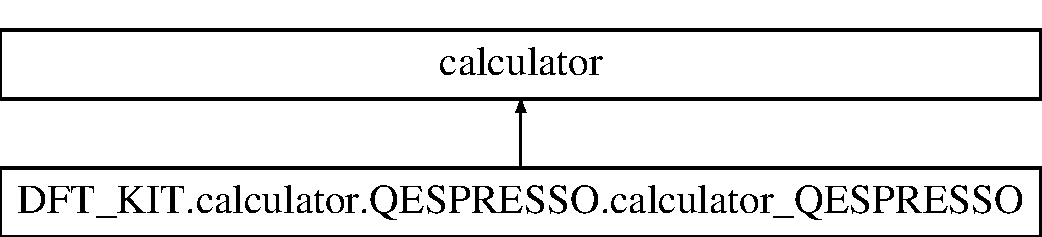
\includegraphics[height=2.000000cm]{class_d_f_t___k_i_t_1_1calculator_1_1_q_e_s_p_r_e_s_s_o_1_1calculator___q_e_s_p_r_e_s_s_o}
\end{center}
\end{figure}
\subsection*{Public Member Functions}
\begin{DoxyCompactItemize}
\item 
def \hyperlink{class_d_f_t___k_i_t_1_1calculator_1_1_q_e_s_p_r_e_s_s_o_1_1calculator___q_e_s_p_r_e_s_s_o_a1e7a766f5475fb690e82742f8c89378e}{\+\_\+\+\_\+init\+\_\+\+\_\+}
\item 
def \hyperlink{class_d_f_t___k_i_t_1_1calculator_1_1_q_e_s_p_r_e_s_s_o_1_1calculator___q_e_s_p_r_e_s_s_o_a6763d0e90887ebb2b733e12fa8a59b1b}{apply\+\_\+scheme}
\item 
def \hyperlink{class_d_f_t___k_i_t_1_1calculator_1_1_q_e_s_p_r_e_s_s_o_1_1calculator___q_e_s_p_r_e_s_s_o_a169a6c16b4b558ad46353a670ebedd09}{run\+\_\+main}
\item 
def \hyperlink{class_d_f_t___k_i_t_1_1calculator_1_1_q_e_s_p_r_e_s_s_o_1_1calculator___q_e_s_p_r_e_s_s_o_abc5b0dc259dd3413a21b3ba51177bd6a}{qes\+\_\+generate\+\_\+pw2wan}
\item 
def \hyperlink{class_d_f_t___k_i_t_1_1calculator_1_1_q_e_s_p_r_e_s_s_o_1_1calculator___q_e_s_p_r_e_s_s_o_adab77a2703ca8c426b3be4113aaa9ce1}{generate\+\_\+files}
\item 
def \hyperlink{class_d_f_t___k_i_t_1_1calculator_1_1_q_e_s_p_r_e_s_s_o_1_1calculator___q_e_s_p_r_e_s_s_o_a40d5c29ed317a18929aab003f1886d47}{qespresso\+\_\+postana\+\_\+xml}
\item 
def \hyperlink{class_d_f_t___k_i_t_1_1calculator_1_1_q_e_s_p_r_e_s_s_o_1_1calculator___q_e_s_p_r_e_s_s_o_a44775813eb4e7b124720d93f9ec092a8}{post\+\_\+process}
\item 
def \hyperlink{class_d_f_t___k_i_t_1_1calculator_1_1_q_e_s_p_r_e_s_s_o_1_1calculator___q_e_s_p_r_e_s_s_o_a67b1814269d3ededf07dbd0516647d2b}{run\+\_\+wannier}
\end{DoxyCompactItemize}
\subsection*{Public Attributes}
\begin{DoxyCompactItemize}
\item 
\hyperlink{class_d_f_t___k_i_t_1_1calculator_1_1_q_e_s_p_r_e_s_s_o_1_1calculator___q_e_s_p_r_e_s_s_o_a592277136beac440bab01bf76b843c2e}{wannier90\+\_\+analysis}
\item 
\hyperlink{class_d_f_t___k_i_t_1_1calculator_1_1_q_e_s_p_r_e_s_s_o_1_1calculator___q_e_s_p_r_e_s_s_o_a5777156c6b8e7acf49acaaefb29dc014}{write\+\_\+occupations}
\item 
\hyperlink{class_d_f_t___k_i_t_1_1calculator_1_1_q_e_s_p_r_e_s_s_o_1_1calculator___q_e_s_p_r_e_s_s_o_ac3dc7e099761294cc4fc50a9d56de21b}{write\+\_\+constraints}
\item 
\hyperlink{class_d_f_t___k_i_t_1_1calculator_1_1_q_e_s_p_r_e_s_s_o_1_1calculator___q_e_s_p_r_e_s_s_o_ad4f633886d1b745fec03b1b18397da75}{write\+\_\+atomic\+\_\+forces}
\item 
\hyperlink{class_d_f_t___k_i_t_1_1calculator_1_1_q_e_s_p_r_e_s_s_o_1_1calculator___q_e_s_p_r_e_s_s_o_a46e4b3b7b81088b086beb9cd5cd64c3c}{atomic\+\_\+positions\+\_\+ang}
\end{DoxyCompactItemize}


\subsection{Detailed Description}


Definition at line 29 of file Q\+E\+S\+P\+R\+E\+S\+S\+O.\+py.



\subsection{Constructor \& Destructor Documentation}
\hypertarget{class_d_f_t___k_i_t_1_1calculator_1_1_q_e_s_p_r_e_s_s_o_1_1calculator___q_e_s_p_r_e_s_s_o_a1e7a766f5475fb690e82742f8c89378e}{\index{D\+F\+T\+\_\+\+K\+I\+T\+::calculator\+::\+Q\+E\+S\+P\+R\+E\+S\+S\+O\+::calculator\+\_\+\+Q\+E\+S\+P\+R\+E\+S\+S\+O@{D\+F\+T\+\_\+\+K\+I\+T\+::calculator\+::\+Q\+E\+S\+P\+R\+E\+S\+S\+O\+::calculator\+\_\+\+Q\+E\+S\+P\+R\+E\+S\+S\+O}!\+\_\+\+\_\+init\+\_\+\+\_\+@{\+\_\+\+\_\+init\+\_\+\+\_\+}}
\index{\+\_\+\+\_\+init\+\_\+\+\_\+@{\+\_\+\+\_\+init\+\_\+\+\_\+}!D\+F\+T\+\_\+\+K\+I\+T\+::calculator\+::\+Q\+E\+S\+P\+R\+E\+S\+S\+O\+::calculator\+\_\+\+Q\+E\+S\+P\+R\+E\+S\+S\+O@{D\+F\+T\+\_\+\+K\+I\+T\+::calculator\+::\+Q\+E\+S\+P\+R\+E\+S\+S\+O\+::calculator\+\_\+\+Q\+E\+S\+P\+R\+E\+S\+S\+O}}
\subsubsection[{\+\_\+\+\_\+init\+\_\+\+\_\+}]{\setlength{\rightskip}{0pt plus 5cm}def D\+F\+T\+\_\+\+K\+I\+T.\+calculator.\+Q\+E\+S\+P\+R\+E\+S\+S\+O.\+calculator\+\_\+\+Q\+E\+S\+P\+R\+E\+S\+S\+O.\+\_\+\+\_\+init\+\_\+\+\_\+ (
\begin{DoxyParamCaption}
\item[{}]{self, }
\item[{}]{postprocess, }
\item[{}]{dft\+\_\+job, }
\item[{}]{crystal, }
\item[{}]{kgrid, }
\item[{}]{scheme = {\ttfamily 0}, }
\item[{}]{parms}
\end{DoxyParamCaption}
)}}\label{class_d_f_t___k_i_t_1_1calculator_1_1_q_e_s_p_r_e_s_s_o_1_1calculator___q_e_s_p_r_e_s_s_o_a1e7a766f5475fb690e82742f8c89378e}


Definition at line 30 of file Q\+E\+S\+P\+R\+E\+S\+S\+O.\+py.



\subsection{Member Function Documentation}
\hypertarget{class_d_f_t___k_i_t_1_1calculator_1_1_q_e_s_p_r_e_s_s_o_1_1calculator___q_e_s_p_r_e_s_s_o_a6763d0e90887ebb2b733e12fa8a59b1b}{\index{D\+F\+T\+\_\+\+K\+I\+T\+::calculator\+::\+Q\+E\+S\+P\+R\+E\+S\+S\+O\+::calculator\+\_\+\+Q\+E\+S\+P\+R\+E\+S\+S\+O@{D\+F\+T\+\_\+\+K\+I\+T\+::calculator\+::\+Q\+E\+S\+P\+R\+E\+S\+S\+O\+::calculator\+\_\+\+Q\+E\+S\+P\+R\+E\+S\+S\+O}!apply\+\_\+scheme@{apply\+\_\+scheme}}
\index{apply\+\_\+scheme@{apply\+\_\+scheme}!D\+F\+T\+\_\+\+K\+I\+T\+::calculator\+::\+Q\+E\+S\+P\+R\+E\+S\+S\+O\+::calculator\+\_\+\+Q\+E\+S\+P\+R\+E\+S\+S\+O@{D\+F\+T\+\_\+\+K\+I\+T\+::calculator\+::\+Q\+E\+S\+P\+R\+E\+S\+S\+O\+::calculator\+\_\+\+Q\+E\+S\+P\+R\+E\+S\+S\+O}}
\subsubsection[{apply\+\_\+scheme}]{\setlength{\rightskip}{0pt plus 5cm}def D\+F\+T\+\_\+\+K\+I\+T.\+calculator.\+Q\+E\+S\+P\+R\+E\+S\+S\+O.\+calculator\+\_\+\+Q\+E\+S\+P\+R\+E\+S\+S\+O.\+apply\+\_\+scheme (
\begin{DoxyParamCaption}
\item[{}]{self, }
\item[{}]{scheme}
\end{DoxyParamCaption}
)}}\label{class_d_f_t___k_i_t_1_1calculator_1_1_q_e_s_p_r_e_s_s_o_1_1calculator___q_e_s_p_r_e_s_s_o_a6763d0e90887ebb2b733e12fa8a59b1b}


Definition at line 39 of file Q\+E\+S\+P\+R\+E\+S\+S\+O.\+py.

\hypertarget{class_d_f_t___k_i_t_1_1calculator_1_1_q_e_s_p_r_e_s_s_o_1_1calculator___q_e_s_p_r_e_s_s_o_adab77a2703ca8c426b3be4113aaa9ce1}{\index{D\+F\+T\+\_\+\+K\+I\+T\+::calculator\+::\+Q\+E\+S\+P\+R\+E\+S\+S\+O\+::calculator\+\_\+\+Q\+E\+S\+P\+R\+E\+S\+S\+O@{D\+F\+T\+\_\+\+K\+I\+T\+::calculator\+::\+Q\+E\+S\+P\+R\+E\+S\+S\+O\+::calculator\+\_\+\+Q\+E\+S\+P\+R\+E\+S\+S\+O}!generate\+\_\+files@{generate\+\_\+files}}
\index{generate\+\_\+files@{generate\+\_\+files}!D\+F\+T\+\_\+\+K\+I\+T\+::calculator\+::\+Q\+E\+S\+P\+R\+E\+S\+S\+O\+::calculator\+\_\+\+Q\+E\+S\+P\+R\+E\+S\+S\+O@{D\+F\+T\+\_\+\+K\+I\+T\+::calculator\+::\+Q\+E\+S\+P\+R\+E\+S\+S\+O\+::calculator\+\_\+\+Q\+E\+S\+P\+R\+E\+S\+S\+O}}
\subsubsection[{generate\+\_\+files}]{\setlength{\rightskip}{0pt plus 5cm}def D\+F\+T\+\_\+\+K\+I\+T.\+calculator.\+Q\+E\+S\+P\+R\+E\+S\+S\+O.\+calculator\+\_\+\+Q\+E\+S\+P\+R\+E\+S\+S\+O.\+generate\+\_\+files (
\begin{DoxyParamCaption}
\item[{}]{self}
\end{DoxyParamCaption}
)}}\label{class_d_f_t___k_i_t_1_1calculator_1_1_q_e_s_p_r_e_s_s_o_1_1calculator___q_e_s_p_r_e_s_s_o_adab77a2703ca8c426b3be4113aaa9ce1}


Definition at line 87 of file Q\+E\+S\+P\+R\+E\+S\+S\+O.\+py.

\hypertarget{class_d_f_t___k_i_t_1_1calculator_1_1_q_e_s_p_r_e_s_s_o_1_1calculator___q_e_s_p_r_e_s_s_o_a44775813eb4e7b124720d93f9ec092a8}{\index{D\+F\+T\+\_\+\+K\+I\+T\+::calculator\+::\+Q\+E\+S\+P\+R\+E\+S\+S\+O\+::calculator\+\_\+\+Q\+E\+S\+P\+R\+E\+S\+S\+O@{D\+F\+T\+\_\+\+K\+I\+T\+::calculator\+::\+Q\+E\+S\+P\+R\+E\+S\+S\+O\+::calculator\+\_\+\+Q\+E\+S\+P\+R\+E\+S\+S\+O}!post\+\_\+process@{post\+\_\+process}}
\index{post\+\_\+process@{post\+\_\+process}!D\+F\+T\+\_\+\+K\+I\+T\+::calculator\+::\+Q\+E\+S\+P\+R\+E\+S\+S\+O\+::calculator\+\_\+\+Q\+E\+S\+P\+R\+E\+S\+S\+O@{D\+F\+T\+\_\+\+K\+I\+T\+::calculator\+::\+Q\+E\+S\+P\+R\+E\+S\+S\+O\+::calculator\+\_\+\+Q\+E\+S\+P\+R\+E\+S\+S\+O}}
\subsubsection[{post\+\_\+process}]{\setlength{\rightskip}{0pt plus 5cm}def D\+F\+T\+\_\+\+K\+I\+T.\+calculator.\+Q\+E\+S\+P\+R\+E\+S\+S\+O.\+calculator\+\_\+\+Q\+E\+S\+P\+R\+E\+S\+S\+O.\+post\+\_\+process (
\begin{DoxyParamCaption}
\item[{}]{self}
\end{DoxyParamCaption}
)}}\label{class_d_f_t___k_i_t_1_1calculator_1_1_q_e_s_p_r_e_s_s_o_1_1calculator___q_e_s_p_r_e_s_s_o_a44775813eb4e7b124720d93f9ec092a8}


Definition at line 224 of file Q\+E\+S\+P\+R\+E\+S\+S\+O.\+py.

\hypertarget{class_d_f_t___k_i_t_1_1calculator_1_1_q_e_s_p_r_e_s_s_o_1_1calculator___q_e_s_p_r_e_s_s_o_abc5b0dc259dd3413a21b3ba51177bd6a}{\index{D\+F\+T\+\_\+\+K\+I\+T\+::calculator\+::\+Q\+E\+S\+P\+R\+E\+S\+S\+O\+::calculator\+\_\+\+Q\+E\+S\+P\+R\+E\+S\+S\+O@{D\+F\+T\+\_\+\+K\+I\+T\+::calculator\+::\+Q\+E\+S\+P\+R\+E\+S\+S\+O\+::calculator\+\_\+\+Q\+E\+S\+P\+R\+E\+S\+S\+O}!qes\+\_\+generate\+\_\+pw2wan@{qes\+\_\+generate\+\_\+pw2wan}}
\index{qes\+\_\+generate\+\_\+pw2wan@{qes\+\_\+generate\+\_\+pw2wan}!D\+F\+T\+\_\+\+K\+I\+T\+::calculator\+::\+Q\+E\+S\+P\+R\+E\+S\+S\+O\+::calculator\+\_\+\+Q\+E\+S\+P\+R\+E\+S\+S\+O@{D\+F\+T\+\_\+\+K\+I\+T\+::calculator\+::\+Q\+E\+S\+P\+R\+E\+S\+S\+O\+::calculator\+\_\+\+Q\+E\+S\+P\+R\+E\+S\+S\+O}}
\subsubsection[{qes\+\_\+generate\+\_\+pw2wan}]{\setlength{\rightskip}{0pt plus 5cm}def D\+F\+T\+\_\+\+K\+I\+T.\+calculator.\+Q\+E\+S\+P\+R\+E\+S\+S\+O.\+calculator\+\_\+\+Q\+E\+S\+P\+R\+E\+S\+S\+O.\+qes\+\_\+generate\+\_\+pw2wan (
\begin{DoxyParamCaption}
\item[{}]{self}
\end{DoxyParamCaption}
)}}\label{class_d_f_t___k_i_t_1_1calculator_1_1_q_e_s_p_r_e_s_s_o_1_1calculator___q_e_s_p_r_e_s_s_o_abc5b0dc259dd3413a21b3ba51177bd6a}


Definition at line 73 of file Q\+E\+S\+P\+R\+E\+S\+S\+O.\+py.

\hypertarget{class_d_f_t___k_i_t_1_1calculator_1_1_q_e_s_p_r_e_s_s_o_1_1calculator___q_e_s_p_r_e_s_s_o_a40d5c29ed317a18929aab003f1886d47}{\index{D\+F\+T\+\_\+\+K\+I\+T\+::calculator\+::\+Q\+E\+S\+P\+R\+E\+S\+S\+O\+::calculator\+\_\+\+Q\+E\+S\+P\+R\+E\+S\+S\+O@{D\+F\+T\+\_\+\+K\+I\+T\+::calculator\+::\+Q\+E\+S\+P\+R\+E\+S\+S\+O\+::calculator\+\_\+\+Q\+E\+S\+P\+R\+E\+S\+S\+O}!qespresso\+\_\+postana\+\_\+xml@{qespresso\+\_\+postana\+\_\+xml}}
\index{qespresso\+\_\+postana\+\_\+xml@{qespresso\+\_\+postana\+\_\+xml}!D\+F\+T\+\_\+\+K\+I\+T\+::calculator\+::\+Q\+E\+S\+P\+R\+E\+S\+S\+O\+::calculator\+\_\+\+Q\+E\+S\+P\+R\+E\+S\+S\+O@{D\+F\+T\+\_\+\+K\+I\+T\+::calculator\+::\+Q\+E\+S\+P\+R\+E\+S\+S\+O\+::calculator\+\_\+\+Q\+E\+S\+P\+R\+E\+S\+S\+O}}
\subsubsection[{qespresso\+\_\+postana\+\_\+xml}]{\setlength{\rightskip}{0pt plus 5cm}def D\+F\+T\+\_\+\+K\+I\+T.\+calculator.\+Q\+E\+S\+P\+R\+E\+S\+S\+O.\+calculator\+\_\+\+Q\+E\+S\+P\+R\+E\+S\+S\+O.\+qespresso\+\_\+postana\+\_\+xml (
\begin{DoxyParamCaption}
\item[{}]{self}
\end{DoxyParamCaption}
)}}\label{class_d_f_t___k_i_t_1_1calculator_1_1_q_e_s_p_r_e_s_s_o_1_1calculator___q_e_s_p_r_e_s_s_o_a40d5c29ed317a18929aab003f1886d47}


Definition at line 197 of file Q\+E\+S\+P\+R\+E\+S\+S\+O.\+py.

\hypertarget{class_d_f_t___k_i_t_1_1calculator_1_1_q_e_s_p_r_e_s_s_o_1_1calculator___q_e_s_p_r_e_s_s_o_a169a6c16b4b558ad46353a670ebedd09}{\index{D\+F\+T\+\_\+\+K\+I\+T\+::calculator\+::\+Q\+E\+S\+P\+R\+E\+S\+S\+O\+::calculator\+\_\+\+Q\+E\+S\+P\+R\+E\+S\+S\+O@{D\+F\+T\+\_\+\+K\+I\+T\+::calculator\+::\+Q\+E\+S\+P\+R\+E\+S\+S\+O\+::calculator\+\_\+\+Q\+E\+S\+P\+R\+E\+S\+S\+O}!run\+\_\+main@{run\+\_\+main}}
\index{run\+\_\+main@{run\+\_\+main}!D\+F\+T\+\_\+\+K\+I\+T\+::calculator\+::\+Q\+E\+S\+P\+R\+E\+S\+S\+O\+::calculator\+\_\+\+Q\+E\+S\+P\+R\+E\+S\+S\+O@{D\+F\+T\+\_\+\+K\+I\+T\+::calculator\+::\+Q\+E\+S\+P\+R\+E\+S\+S\+O\+::calculator\+\_\+\+Q\+E\+S\+P\+R\+E\+S\+S\+O}}
\subsubsection[{run\+\_\+main}]{\setlength{\rightskip}{0pt plus 5cm}def D\+F\+T\+\_\+\+K\+I\+T.\+calculator.\+Q\+E\+S\+P\+R\+E\+S\+S\+O.\+calculator\+\_\+\+Q\+E\+S\+P\+R\+E\+S\+S\+O.\+run\+\_\+main (
\begin{DoxyParamCaption}
\item[{}]{self}
\end{DoxyParamCaption}
)}}\label{class_d_f_t___k_i_t_1_1calculator_1_1_q_e_s_p_r_e_s_s_o_1_1calculator___q_e_s_p_r_e_s_s_o_a169a6c16b4b558ad46353a670ebedd09}


Definition at line 68 of file Q\+E\+S\+P\+R\+E\+S\+S\+O.\+py.

\hypertarget{class_d_f_t___k_i_t_1_1calculator_1_1_q_e_s_p_r_e_s_s_o_1_1calculator___q_e_s_p_r_e_s_s_o_a67b1814269d3ededf07dbd0516647d2b}{\index{D\+F\+T\+\_\+\+K\+I\+T\+::calculator\+::\+Q\+E\+S\+P\+R\+E\+S\+S\+O\+::calculator\+\_\+\+Q\+E\+S\+P\+R\+E\+S\+S\+O@{D\+F\+T\+\_\+\+K\+I\+T\+::calculator\+::\+Q\+E\+S\+P\+R\+E\+S\+S\+O\+::calculator\+\_\+\+Q\+E\+S\+P\+R\+E\+S\+S\+O}!run\+\_\+wannier@{run\+\_\+wannier}}
\index{run\+\_\+wannier@{run\+\_\+wannier}!D\+F\+T\+\_\+\+K\+I\+T\+::calculator\+::\+Q\+E\+S\+P\+R\+E\+S\+S\+O\+::calculator\+\_\+\+Q\+E\+S\+P\+R\+E\+S\+S\+O@{D\+F\+T\+\_\+\+K\+I\+T\+::calculator\+::\+Q\+E\+S\+P\+R\+E\+S\+S\+O\+::calculator\+\_\+\+Q\+E\+S\+P\+R\+E\+S\+S\+O}}
\subsubsection[{run\+\_\+wannier}]{\setlength{\rightskip}{0pt plus 5cm}def D\+F\+T\+\_\+\+K\+I\+T.\+calculator.\+Q\+E\+S\+P\+R\+E\+S\+S\+O.\+calculator\+\_\+\+Q\+E\+S\+P\+R\+E\+S\+S\+O.\+run\+\_\+wannier (
\begin{DoxyParamCaption}
\item[{}]{self}
\end{DoxyParamCaption}
)}}\label{class_d_f_t___k_i_t_1_1calculator_1_1_q_e_s_p_r_e_s_s_o_1_1calculator___q_e_s_p_r_e_s_s_o_a67b1814269d3ededf07dbd0516647d2b}


Definition at line 227 of file Q\+E\+S\+P\+R\+E\+S\+S\+O.\+py.



\subsection{Member Data Documentation}
\hypertarget{class_d_f_t___k_i_t_1_1calculator_1_1_q_e_s_p_r_e_s_s_o_1_1calculator___q_e_s_p_r_e_s_s_o_a46e4b3b7b81088b086beb9cd5cd64c3c}{\index{D\+F\+T\+\_\+\+K\+I\+T\+::calculator\+::\+Q\+E\+S\+P\+R\+E\+S\+S\+O\+::calculator\+\_\+\+Q\+E\+S\+P\+R\+E\+S\+S\+O@{D\+F\+T\+\_\+\+K\+I\+T\+::calculator\+::\+Q\+E\+S\+P\+R\+E\+S\+S\+O\+::calculator\+\_\+\+Q\+E\+S\+P\+R\+E\+S\+S\+O}!atomic\+\_\+positions\+\_\+ang@{atomic\+\_\+positions\+\_\+ang}}
\index{atomic\+\_\+positions\+\_\+ang@{atomic\+\_\+positions\+\_\+ang}!D\+F\+T\+\_\+\+K\+I\+T\+::calculator\+::\+Q\+E\+S\+P\+R\+E\+S\+S\+O\+::calculator\+\_\+\+Q\+E\+S\+P\+R\+E\+S\+S\+O@{D\+F\+T\+\_\+\+K\+I\+T\+::calculator\+::\+Q\+E\+S\+P\+R\+E\+S\+S\+O\+::calculator\+\_\+\+Q\+E\+S\+P\+R\+E\+S\+S\+O}}
\subsubsection[{atomic\+\_\+positions\+\_\+ang}]{\setlength{\rightskip}{0pt plus 5cm}D\+F\+T\+\_\+\+K\+I\+T.\+calculator.\+Q\+E\+S\+P\+R\+E\+S\+S\+O.\+calculator\+\_\+\+Q\+E\+S\+P\+R\+E\+S\+S\+O.\+atomic\+\_\+positions\+\_\+ang}}\label{class_d_f_t___k_i_t_1_1calculator_1_1_q_e_s_p_r_e_s_s_o_1_1calculator___q_e_s_p_r_e_s_s_o_a46e4b3b7b81088b086beb9cd5cd64c3c}


Definition at line 37 of file Q\+E\+S\+P\+R\+E\+S\+S\+O.\+py.

\hypertarget{class_d_f_t___k_i_t_1_1calculator_1_1_q_e_s_p_r_e_s_s_o_1_1calculator___q_e_s_p_r_e_s_s_o_a592277136beac440bab01bf76b843c2e}{\index{D\+F\+T\+\_\+\+K\+I\+T\+::calculator\+::\+Q\+E\+S\+P\+R\+E\+S\+S\+O\+::calculator\+\_\+\+Q\+E\+S\+P\+R\+E\+S\+S\+O@{D\+F\+T\+\_\+\+K\+I\+T\+::calculator\+::\+Q\+E\+S\+P\+R\+E\+S\+S\+O\+::calculator\+\_\+\+Q\+E\+S\+P\+R\+E\+S\+S\+O}!wannier90\+\_\+analysis@{wannier90\+\_\+analysis}}
\index{wannier90\+\_\+analysis@{wannier90\+\_\+analysis}!D\+F\+T\+\_\+\+K\+I\+T\+::calculator\+::\+Q\+E\+S\+P\+R\+E\+S\+S\+O\+::calculator\+\_\+\+Q\+E\+S\+P\+R\+E\+S\+S\+O@{D\+F\+T\+\_\+\+K\+I\+T\+::calculator\+::\+Q\+E\+S\+P\+R\+E\+S\+S\+O\+::calculator\+\_\+\+Q\+E\+S\+P\+R\+E\+S\+S\+O}}
\subsubsection[{wannier90\+\_\+analysis}]{\setlength{\rightskip}{0pt plus 5cm}D\+F\+T\+\_\+\+K\+I\+T.\+calculator.\+Q\+E\+S\+P\+R\+E\+S\+S\+O.\+calculator\+\_\+\+Q\+E\+S\+P\+R\+E\+S\+S\+O.\+wannier90\+\_\+analysis}}\label{class_d_f_t___k_i_t_1_1calculator_1_1_q_e_s_p_r_e_s_s_o_1_1calculator___q_e_s_p_r_e_s_s_o_a592277136beac440bab01bf76b843c2e}


Definition at line 33 of file Q\+E\+S\+P\+R\+E\+S\+S\+O.\+py.

\hypertarget{class_d_f_t___k_i_t_1_1calculator_1_1_q_e_s_p_r_e_s_s_o_1_1calculator___q_e_s_p_r_e_s_s_o_ad4f633886d1b745fec03b1b18397da75}{\index{D\+F\+T\+\_\+\+K\+I\+T\+::calculator\+::\+Q\+E\+S\+P\+R\+E\+S\+S\+O\+::calculator\+\_\+\+Q\+E\+S\+P\+R\+E\+S\+S\+O@{D\+F\+T\+\_\+\+K\+I\+T\+::calculator\+::\+Q\+E\+S\+P\+R\+E\+S\+S\+O\+::calculator\+\_\+\+Q\+E\+S\+P\+R\+E\+S\+S\+O}!write\+\_\+atomic\+\_\+forces@{write\+\_\+atomic\+\_\+forces}}
\index{write\+\_\+atomic\+\_\+forces@{write\+\_\+atomic\+\_\+forces}!D\+F\+T\+\_\+\+K\+I\+T\+::calculator\+::\+Q\+E\+S\+P\+R\+E\+S\+S\+O\+::calculator\+\_\+\+Q\+E\+S\+P\+R\+E\+S\+S\+O@{D\+F\+T\+\_\+\+K\+I\+T\+::calculator\+::\+Q\+E\+S\+P\+R\+E\+S\+S\+O\+::calculator\+\_\+\+Q\+E\+S\+P\+R\+E\+S\+S\+O}}
\subsubsection[{write\+\_\+atomic\+\_\+forces}]{\setlength{\rightskip}{0pt plus 5cm}D\+F\+T\+\_\+\+K\+I\+T.\+calculator.\+Q\+E\+S\+P\+R\+E\+S\+S\+O.\+calculator\+\_\+\+Q\+E\+S\+P\+R\+E\+S\+S\+O.\+write\+\_\+atomic\+\_\+forces}}\label{class_d_f_t___k_i_t_1_1calculator_1_1_q_e_s_p_r_e_s_s_o_1_1calculator___q_e_s_p_r_e_s_s_o_ad4f633886d1b745fec03b1b18397da75}


Definition at line 36 of file Q\+E\+S\+P\+R\+E\+S\+S\+O.\+py.

\hypertarget{class_d_f_t___k_i_t_1_1calculator_1_1_q_e_s_p_r_e_s_s_o_1_1calculator___q_e_s_p_r_e_s_s_o_ac3dc7e099761294cc4fc50a9d56de21b}{\index{D\+F\+T\+\_\+\+K\+I\+T\+::calculator\+::\+Q\+E\+S\+P\+R\+E\+S\+S\+O\+::calculator\+\_\+\+Q\+E\+S\+P\+R\+E\+S\+S\+O@{D\+F\+T\+\_\+\+K\+I\+T\+::calculator\+::\+Q\+E\+S\+P\+R\+E\+S\+S\+O\+::calculator\+\_\+\+Q\+E\+S\+P\+R\+E\+S\+S\+O}!write\+\_\+constraints@{write\+\_\+constraints}}
\index{write\+\_\+constraints@{write\+\_\+constraints}!D\+F\+T\+\_\+\+K\+I\+T\+::calculator\+::\+Q\+E\+S\+P\+R\+E\+S\+S\+O\+::calculator\+\_\+\+Q\+E\+S\+P\+R\+E\+S\+S\+O@{D\+F\+T\+\_\+\+K\+I\+T\+::calculator\+::\+Q\+E\+S\+P\+R\+E\+S\+S\+O\+::calculator\+\_\+\+Q\+E\+S\+P\+R\+E\+S\+S\+O}}
\subsubsection[{write\+\_\+constraints}]{\setlength{\rightskip}{0pt plus 5cm}D\+F\+T\+\_\+\+K\+I\+T.\+calculator.\+Q\+E\+S\+P\+R\+E\+S\+S\+O.\+calculator\+\_\+\+Q\+E\+S\+P\+R\+E\+S\+S\+O.\+write\+\_\+constraints}}\label{class_d_f_t___k_i_t_1_1calculator_1_1_q_e_s_p_r_e_s_s_o_1_1calculator___q_e_s_p_r_e_s_s_o_ac3dc7e099761294cc4fc50a9d56de21b}


Definition at line 35 of file Q\+E\+S\+P\+R\+E\+S\+S\+O.\+py.

\hypertarget{class_d_f_t___k_i_t_1_1calculator_1_1_q_e_s_p_r_e_s_s_o_1_1calculator___q_e_s_p_r_e_s_s_o_a5777156c6b8e7acf49acaaefb29dc014}{\index{D\+F\+T\+\_\+\+K\+I\+T\+::calculator\+::\+Q\+E\+S\+P\+R\+E\+S\+S\+O\+::calculator\+\_\+\+Q\+E\+S\+P\+R\+E\+S\+S\+O@{D\+F\+T\+\_\+\+K\+I\+T\+::calculator\+::\+Q\+E\+S\+P\+R\+E\+S\+S\+O\+::calculator\+\_\+\+Q\+E\+S\+P\+R\+E\+S\+S\+O}!write\+\_\+occupations@{write\+\_\+occupations}}
\index{write\+\_\+occupations@{write\+\_\+occupations}!D\+F\+T\+\_\+\+K\+I\+T\+::calculator\+::\+Q\+E\+S\+P\+R\+E\+S\+S\+O\+::calculator\+\_\+\+Q\+E\+S\+P\+R\+E\+S\+S\+O@{D\+F\+T\+\_\+\+K\+I\+T\+::calculator\+::\+Q\+E\+S\+P\+R\+E\+S\+S\+O\+::calculator\+\_\+\+Q\+E\+S\+P\+R\+E\+S\+S\+O}}
\subsubsection[{write\+\_\+occupations}]{\setlength{\rightskip}{0pt plus 5cm}D\+F\+T\+\_\+\+K\+I\+T.\+calculator.\+Q\+E\+S\+P\+R\+E\+S\+S\+O.\+calculator\+\_\+\+Q\+E\+S\+P\+R\+E\+S\+S\+O.\+write\+\_\+occupations}}\label{class_d_f_t___k_i_t_1_1calculator_1_1_q_e_s_p_r_e_s_s_o_1_1calculator___q_e_s_p_r_e_s_s_o_a5777156c6b8e7acf49acaaefb29dc014}


Definition at line 34 of file Q\+E\+S\+P\+R\+E\+S\+S\+O.\+py.



The documentation for this class was generated from the following file\+:\begin{DoxyCompactItemize}
\item 
calculator/\hyperlink{_q_e_s_p_r_e_s_s_o_8py}{Q\+E\+S\+P\+R\+E\+S\+S\+O.\+py}\end{DoxyCompactItemize}

\hypertarget{class_d_f_t___k_i_t_1_1calculator_1_1script_1_1calculator__script}{\section{D\+F\+T\+\_\+\+K\+I\+T.\+calculator.\+script.\+calculator\+\_\+script Class Reference}
\label{class_d_f_t___k_i_t_1_1calculator_1_1script_1_1calculator__script}\index{D\+F\+T\+\_\+\+K\+I\+T.\+calculator.\+script.\+calculator\+\_\+script@{D\+F\+T\+\_\+\+K\+I\+T.\+calculator.\+script.\+calculator\+\_\+script}}
}
Inheritance diagram for D\+F\+T\+\_\+\+K\+I\+T.\+calculator.\+script.\+calculator\+\_\+script\+:\begin{figure}[H]
\begin{center}
\leavevmode
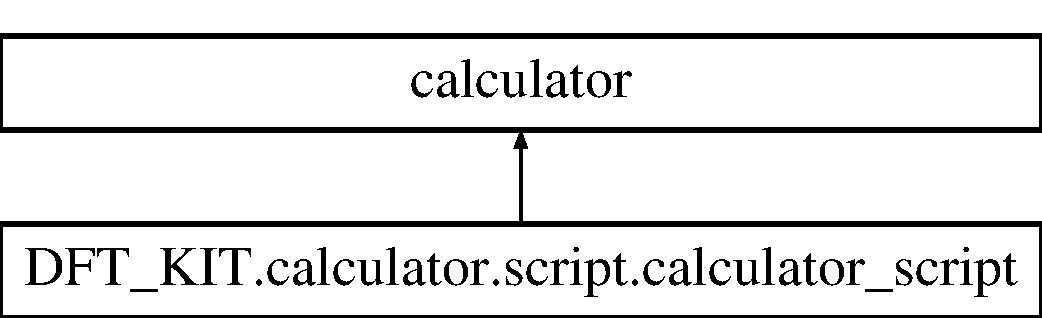
\includegraphics[height=2.000000cm]{class_d_f_t___k_i_t_1_1calculator_1_1script_1_1calculator__script}
\end{center}
\end{figure}
\subsection*{Public Member Functions}
\begin{DoxyCompactItemize}
\item 
def \hyperlink{class_d_f_t___k_i_t_1_1calculator_1_1script_1_1calculator__script_a79031df5c45b2f4ed5c692147f8ec27d}{\+\_\+\+\_\+init\+\_\+\+\_\+}
\item 
def \hyperlink{class_d_f_t___k_i_t_1_1calculator_1_1script_1_1calculator__script_a0cd1d0bc8e1ddbe9603ff68c83cb223b}{run\+\_\+main}
\item 
def \hyperlink{class_d_f_t___k_i_t_1_1calculator_1_1script_1_1calculator__script_a1242143a8e3270990a905ac548dc0203}{generate\+\_\+files}
\item 
def \hyperlink{class_d_f_t___k_i_t_1_1calculator_1_1script_1_1calculator__script_a85e472b18c63e3ede5d4e1a140bc4835}{post\+\_\+process}
\end{DoxyCompactItemize}


\subsection{Detailed Description}


Definition at line 30 of file script.\+py.



\subsection{Constructor \& Destructor Documentation}
\hypertarget{class_d_f_t___k_i_t_1_1calculator_1_1script_1_1calculator__script_a79031df5c45b2f4ed5c692147f8ec27d}{\index{D\+F\+T\+\_\+\+K\+I\+T\+::calculator\+::script\+::calculator\+\_\+script@{D\+F\+T\+\_\+\+K\+I\+T\+::calculator\+::script\+::calculator\+\_\+script}!\+\_\+\+\_\+init\+\_\+\+\_\+@{\+\_\+\+\_\+init\+\_\+\+\_\+}}
\index{\+\_\+\+\_\+init\+\_\+\+\_\+@{\+\_\+\+\_\+init\+\_\+\+\_\+}!D\+F\+T\+\_\+\+K\+I\+T\+::calculator\+::script\+::calculator\+\_\+script@{D\+F\+T\+\_\+\+K\+I\+T\+::calculator\+::script\+::calculator\+\_\+script}}
\subsubsection[{\+\_\+\+\_\+init\+\_\+\+\_\+}]{\setlength{\rightskip}{0pt plus 5cm}def D\+F\+T\+\_\+\+K\+I\+T.\+calculator.\+script.\+calculator\+\_\+script.\+\_\+\+\_\+init\+\_\+\+\_\+ (
\begin{DoxyParamCaption}
\item[{}]{self, }
\item[{}]{postprocess, }
\item[{}]{dft\+\_\+job, }
\item[{}]{crystal, }
\item[{}]{kgrid, }
\item[{}]{parms}
\end{DoxyParamCaption}
)}}\label{class_d_f_t___k_i_t_1_1calculator_1_1script_1_1calculator__script_a79031df5c45b2f4ed5c692147f8ec27d}


Definition at line 31 of file script.\+py.



\subsection{Member Function Documentation}
\hypertarget{class_d_f_t___k_i_t_1_1calculator_1_1script_1_1calculator__script_a1242143a8e3270990a905ac548dc0203}{\index{D\+F\+T\+\_\+\+K\+I\+T\+::calculator\+::script\+::calculator\+\_\+script@{D\+F\+T\+\_\+\+K\+I\+T\+::calculator\+::script\+::calculator\+\_\+script}!generate\+\_\+files@{generate\+\_\+files}}
\index{generate\+\_\+files@{generate\+\_\+files}!D\+F\+T\+\_\+\+K\+I\+T\+::calculator\+::script\+::calculator\+\_\+script@{D\+F\+T\+\_\+\+K\+I\+T\+::calculator\+::script\+::calculator\+\_\+script}}
\subsubsection[{generate\+\_\+files}]{\setlength{\rightskip}{0pt plus 5cm}def D\+F\+T\+\_\+\+K\+I\+T.\+calculator.\+script.\+calculator\+\_\+script.\+generate\+\_\+files (
\begin{DoxyParamCaption}
\item[{}]{self}
\end{DoxyParamCaption}
)}}\label{class_d_f_t___k_i_t_1_1calculator_1_1script_1_1calculator__script_a1242143a8e3270990a905ac548dc0203}


Definition at line 40 of file script.\+py.

\hypertarget{class_d_f_t___k_i_t_1_1calculator_1_1script_1_1calculator__script_a85e472b18c63e3ede5d4e1a140bc4835}{\index{D\+F\+T\+\_\+\+K\+I\+T\+::calculator\+::script\+::calculator\+\_\+script@{D\+F\+T\+\_\+\+K\+I\+T\+::calculator\+::script\+::calculator\+\_\+script}!post\+\_\+process@{post\+\_\+process}}
\index{post\+\_\+process@{post\+\_\+process}!D\+F\+T\+\_\+\+K\+I\+T\+::calculator\+::script\+::calculator\+\_\+script@{D\+F\+T\+\_\+\+K\+I\+T\+::calculator\+::script\+::calculator\+\_\+script}}
\subsubsection[{post\+\_\+process}]{\setlength{\rightskip}{0pt plus 5cm}def D\+F\+T\+\_\+\+K\+I\+T.\+calculator.\+script.\+calculator\+\_\+script.\+post\+\_\+process (
\begin{DoxyParamCaption}
\item[{}]{self}
\end{DoxyParamCaption}
)}}\label{class_d_f_t___k_i_t_1_1calculator_1_1script_1_1calculator__script_a85e472b18c63e3ede5d4e1a140bc4835}


Definition at line 44 of file script.\+py.

\hypertarget{class_d_f_t___k_i_t_1_1calculator_1_1script_1_1calculator__script_a0cd1d0bc8e1ddbe9603ff68c83cb223b}{\index{D\+F\+T\+\_\+\+K\+I\+T\+::calculator\+::script\+::calculator\+\_\+script@{D\+F\+T\+\_\+\+K\+I\+T\+::calculator\+::script\+::calculator\+\_\+script}!run\+\_\+main@{run\+\_\+main}}
\index{run\+\_\+main@{run\+\_\+main}!D\+F\+T\+\_\+\+K\+I\+T\+::calculator\+::script\+::calculator\+\_\+script@{D\+F\+T\+\_\+\+K\+I\+T\+::calculator\+::script\+::calculator\+\_\+script}}
\subsubsection[{run\+\_\+main}]{\setlength{\rightskip}{0pt plus 5cm}def D\+F\+T\+\_\+\+K\+I\+T.\+calculator.\+script.\+calculator\+\_\+script.\+run\+\_\+main (
\begin{DoxyParamCaption}
\item[{}]{self}
\end{DoxyParamCaption}
)}}\label{class_d_f_t___k_i_t_1_1calculator_1_1script_1_1calculator__script_a0cd1d0bc8e1ddbe9603ff68c83cb223b}


Definition at line 36 of file script.\+py.



The documentation for this class was generated from the following file\+:\begin{DoxyCompactItemize}
\item 
calculator/\hyperlink{script_8py}{script.\+py}\end{DoxyCompactItemize}

\hypertarget{class_d_f_t___k_i_t_1_1calculator_1_1_s_i_e_s_t_a_1_1calculator___s_i_e_s_t_a}{\section{D\+F\+T\+\_\+\+K\+I\+T.\+calculator.\+S\+I\+E\+S\+T\+A.\+calculator\+\_\+\+S\+I\+E\+S\+T\+A Class Reference}
\label{class_d_f_t___k_i_t_1_1calculator_1_1_s_i_e_s_t_a_1_1calculator___s_i_e_s_t_a}\index{D\+F\+T\+\_\+\+K\+I\+T.\+calculator.\+S\+I\+E\+S\+T\+A.\+calculator\+\_\+\+S\+I\+E\+S\+T\+A@{D\+F\+T\+\_\+\+K\+I\+T.\+calculator.\+S\+I\+E\+S\+T\+A.\+calculator\+\_\+\+S\+I\+E\+S\+T\+A}}
}
Inheritance diagram for D\+F\+T\+\_\+\+K\+I\+T.\+calculator.\+S\+I\+E\+S\+T\+A.\+calculator\+\_\+\+S\+I\+E\+S\+T\+A\+:\begin{figure}[H]
\begin{center}
\leavevmode
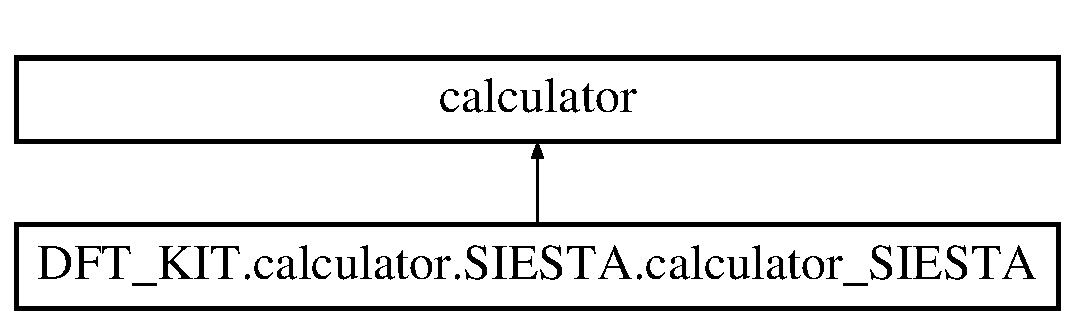
\includegraphics[height=2.000000cm]{class_d_f_t___k_i_t_1_1calculator_1_1_s_i_e_s_t_a_1_1calculator___s_i_e_s_t_a}
\end{center}
\end{figure}
\subsection*{Public Member Functions}
\begin{DoxyCompactItemize}
\item 
def \hyperlink{class_d_f_t___k_i_t_1_1calculator_1_1_s_i_e_s_t_a_1_1calculator___s_i_e_s_t_a_aaba365f29a7fc8b7d5bb5bd4c2939fb4}{\+\_\+\+\_\+init\+\_\+\+\_\+}
\item 
def \hyperlink{class_d_f_t___k_i_t_1_1calculator_1_1_s_i_e_s_t_a_1_1calculator___s_i_e_s_t_a_a40571d7e78a280b2016e4532af4efcbc}{apply\+\_\+scheme}
\item 
def \hyperlink{class_d_f_t___k_i_t_1_1calculator_1_1_s_i_e_s_t_a_1_1calculator___s_i_e_s_t_a_a175e5b91be01acff708f9d7be2b1156b}{generate\+\_\+files}
\end{DoxyCompactItemize}


\subsection{Detailed Description}


Definition at line 298 of file S\+I\+E\+S\+T\+A.\+py.



\subsection{Constructor \& Destructor Documentation}
\hypertarget{class_d_f_t___k_i_t_1_1calculator_1_1_s_i_e_s_t_a_1_1calculator___s_i_e_s_t_a_aaba365f29a7fc8b7d5bb5bd4c2939fb4}{\index{D\+F\+T\+\_\+\+K\+I\+T\+::calculator\+::\+S\+I\+E\+S\+T\+A\+::calculator\+\_\+\+S\+I\+E\+S\+T\+A@{D\+F\+T\+\_\+\+K\+I\+T\+::calculator\+::\+S\+I\+E\+S\+T\+A\+::calculator\+\_\+\+S\+I\+E\+S\+T\+A}!\+\_\+\+\_\+init\+\_\+\+\_\+@{\+\_\+\+\_\+init\+\_\+\+\_\+}}
\index{\+\_\+\+\_\+init\+\_\+\+\_\+@{\+\_\+\+\_\+init\+\_\+\+\_\+}!D\+F\+T\+\_\+\+K\+I\+T\+::calculator\+::\+S\+I\+E\+S\+T\+A\+::calculator\+\_\+\+S\+I\+E\+S\+T\+A@{D\+F\+T\+\_\+\+K\+I\+T\+::calculator\+::\+S\+I\+E\+S\+T\+A\+::calculator\+\_\+\+S\+I\+E\+S\+T\+A}}
\subsubsection[{\+\_\+\+\_\+init\+\_\+\+\_\+}]{\setlength{\rightskip}{0pt plus 5cm}def D\+F\+T\+\_\+\+K\+I\+T.\+calculator.\+S\+I\+E\+S\+T\+A.\+calculator\+\_\+\+S\+I\+E\+S\+T\+A.\+\_\+\+\_\+init\+\_\+\+\_\+ (
\begin{DoxyParamCaption}
\item[{}]{self, }
\item[{}]{postprocess, }
\item[{}]{dft\+\_\+job, }
\item[{}]{crystal, }
\item[{}]{kgrid, }
\item[{}]{scheme = {\ttfamily 0}, }
\item[{}]{parms}
\end{DoxyParamCaption}
)}}\label{class_d_f_t___k_i_t_1_1calculator_1_1_s_i_e_s_t_a_1_1calculator___s_i_e_s_t_a_aaba365f29a7fc8b7d5bb5bd4c2939fb4}


Definition at line 299 of file S\+I\+E\+S\+T\+A.\+py.



\subsection{Member Function Documentation}
\hypertarget{class_d_f_t___k_i_t_1_1calculator_1_1_s_i_e_s_t_a_1_1calculator___s_i_e_s_t_a_a40571d7e78a280b2016e4532af4efcbc}{\index{D\+F\+T\+\_\+\+K\+I\+T\+::calculator\+::\+S\+I\+E\+S\+T\+A\+::calculator\+\_\+\+S\+I\+E\+S\+T\+A@{D\+F\+T\+\_\+\+K\+I\+T\+::calculator\+::\+S\+I\+E\+S\+T\+A\+::calculator\+\_\+\+S\+I\+E\+S\+T\+A}!apply\+\_\+scheme@{apply\+\_\+scheme}}
\index{apply\+\_\+scheme@{apply\+\_\+scheme}!D\+F\+T\+\_\+\+K\+I\+T\+::calculator\+::\+S\+I\+E\+S\+T\+A\+::calculator\+\_\+\+S\+I\+E\+S\+T\+A@{D\+F\+T\+\_\+\+K\+I\+T\+::calculator\+::\+S\+I\+E\+S\+T\+A\+::calculator\+\_\+\+S\+I\+E\+S\+T\+A}}
\subsubsection[{apply\+\_\+scheme}]{\setlength{\rightskip}{0pt plus 5cm}def D\+F\+T\+\_\+\+K\+I\+T.\+calculator.\+S\+I\+E\+S\+T\+A.\+calculator\+\_\+\+S\+I\+E\+S\+T\+A.\+apply\+\_\+scheme (
\begin{DoxyParamCaption}
\item[{}]{self, }
\item[{}]{scheme}
\end{DoxyParamCaption}
)}}\label{class_d_f_t___k_i_t_1_1calculator_1_1_s_i_e_s_t_a_1_1calculator___s_i_e_s_t_a_a40571d7e78a280b2016e4532af4efcbc}


Definition at line 302 of file S\+I\+E\+S\+T\+A.\+py.

\hypertarget{class_d_f_t___k_i_t_1_1calculator_1_1_s_i_e_s_t_a_1_1calculator___s_i_e_s_t_a_a175e5b91be01acff708f9d7be2b1156b}{\index{D\+F\+T\+\_\+\+K\+I\+T\+::calculator\+::\+S\+I\+E\+S\+T\+A\+::calculator\+\_\+\+S\+I\+E\+S\+T\+A@{D\+F\+T\+\_\+\+K\+I\+T\+::calculator\+::\+S\+I\+E\+S\+T\+A\+::calculator\+\_\+\+S\+I\+E\+S\+T\+A}!generate\+\_\+files@{generate\+\_\+files}}
\index{generate\+\_\+files@{generate\+\_\+files}!D\+F\+T\+\_\+\+K\+I\+T\+::calculator\+::\+S\+I\+E\+S\+T\+A\+::calculator\+\_\+\+S\+I\+E\+S\+T\+A@{D\+F\+T\+\_\+\+K\+I\+T\+::calculator\+::\+S\+I\+E\+S\+T\+A\+::calculator\+\_\+\+S\+I\+E\+S\+T\+A}}
\subsubsection[{generate\+\_\+files}]{\setlength{\rightskip}{0pt plus 5cm}def D\+F\+T\+\_\+\+K\+I\+T.\+calculator.\+S\+I\+E\+S\+T\+A.\+calculator\+\_\+\+S\+I\+E\+S\+T\+A.\+generate\+\_\+files (
\begin{DoxyParamCaption}
\item[{}]{self}
\end{DoxyParamCaption}
)}}\label{class_d_f_t___k_i_t_1_1calculator_1_1_s_i_e_s_t_a_1_1calculator___s_i_e_s_t_a_a175e5b91be01acff708f9d7be2b1156b}


Definition at line 328 of file S\+I\+E\+S\+T\+A.\+py.



The documentation for this class was generated from the following file\+:\begin{DoxyCompactItemize}
\item 
calculator/\hyperlink{_s_i_e_s_t_a_8py}{S\+I\+E\+S\+T\+A.\+py}\end{DoxyCompactItemize}

\hypertarget{class_d_f_t___k_i_t_1_1calculator_1_1_v_a_s_p_1_1calculator___v_a_s_p}{\section{D\+F\+T\+\_\+\+K\+I\+T.\+calculator.\+V\+A\+S\+P.\+calculator\+\_\+\+V\+A\+S\+P Class Reference}
\label{class_d_f_t___k_i_t_1_1calculator_1_1_v_a_s_p_1_1calculator___v_a_s_p}\index{D\+F\+T\+\_\+\+K\+I\+T.\+calculator.\+V\+A\+S\+P.\+calculator\+\_\+\+V\+A\+S\+P@{D\+F\+T\+\_\+\+K\+I\+T.\+calculator.\+V\+A\+S\+P.\+calculator\+\_\+\+V\+A\+S\+P}}
}
Inheritance diagram for D\+F\+T\+\_\+\+K\+I\+T.\+calculator.\+V\+A\+S\+P.\+calculator\+\_\+\+V\+A\+S\+P\+:\begin{figure}[H]
\begin{center}
\leavevmode
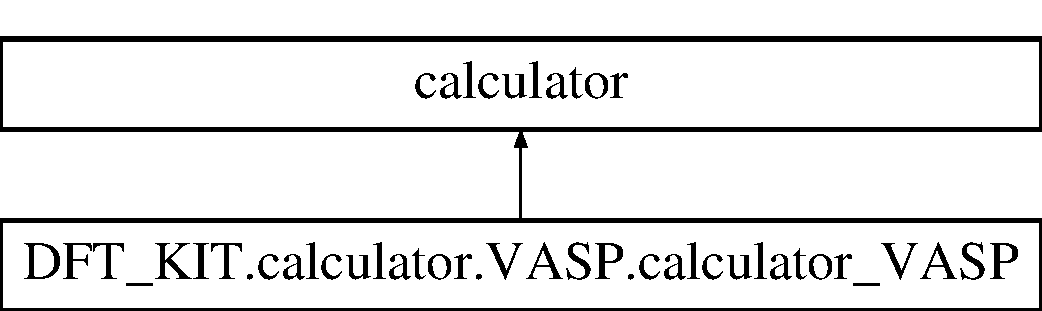
\includegraphics[height=2.000000cm]{class_d_f_t___k_i_t_1_1calculator_1_1_v_a_s_p_1_1calculator___v_a_s_p}
\end{center}
\end{figure}
\subsection*{Public Member Functions}
\begin{DoxyCompactItemize}
\item 
def \hyperlink{class_d_f_t___k_i_t_1_1calculator_1_1_v_a_s_p_1_1calculator___v_a_s_p_aa93fe1d0817f60fec3803e01b395ea29}{\+\_\+\+\_\+init\+\_\+\+\_\+}
\item 
def \hyperlink{class_d_f_t___k_i_t_1_1calculator_1_1_v_a_s_p_1_1calculator___v_a_s_p_a2b324b0463ee70a4771a37aa6602de0f}{set\+\_\+run\+\_\+vasp\+\_\+mode}
\item 
def \hyperlink{class_d_f_t___k_i_t_1_1calculator_1_1_v_a_s_p_1_1calculator___v_a_s_p_a9c42b72766e542209e2a71188c73a05c}{run\+\_\+main}
\item 
def \hyperlink{class_d_f_t___k_i_t_1_1calculator_1_1_v_a_s_p_1_1calculator___v_a_s_p_a14129668e5520b33683f54e1b1b46d48}{generate\+\_\+files}
\item 
def \hyperlink{class_d_f_t___k_i_t_1_1calculator_1_1_v_a_s_p_1_1calculator___v_a_s_p_acaf8bf95391a54226d23ca036375fdc7}{vasp\+\_\+generate\+\_\+incar}
\item 
def \hyperlink{class_d_f_t___k_i_t_1_1calculator_1_1_v_a_s_p_1_1calculator___v_a_s_p_a9faee2a517349479744f59f977a965f2}{vasp\+\_\+generate\+\_\+poscar}
\item 
def \hyperlink{class_d_f_t___k_i_t_1_1calculator_1_1_v_a_s_p_1_1calculator___v_a_s_p_a338715e224e54b8c941ef3348e672a86}{vasp\+\_\+generate\+\_\+kpoints}
\item 
def \hyperlink{class_d_f_t___k_i_t_1_1calculator_1_1_v_a_s_p_1_1calculator___v_a_s_p_a2c3605f1f29f24ed066b69b93ce9c6c3}{apply\+\_\+scheme}
\item 
def \hyperlink{class_d_f_t___k_i_t_1_1calculator_1_1_v_a_s_p_1_1calculator___v_a_s_p_a7ffb25fd49a4631987e84b0bfb41d5cf}{post\+\_\+process}
\item 
def \hyperlink{class_d_f_t___k_i_t_1_1calculator_1_1_v_a_s_p_1_1calculator___v_a_s_p_a4cdeea8dcddf4f9e0b2293803aa5c10a}{vasp\+\_\+load\+\_\+calculation\+\_\+xml}
\item 
def \hyperlink{class_d_f_t___k_i_t_1_1calculator_1_1_v_a_s_p_1_1calculator___v_a_s_p_aadcb71e59295bdf573802252dcc55682}{vasp\+\_\+postana\+\_\+xml}
\item 
def \hyperlink{class_d_f_t___k_i_t_1_1calculator_1_1_v_a_s_p_1_1calculator___v_a_s_p_a084c108ca41f4875f171ddd71265b2f3}{vasp\+\_\+postana\+\_\+calculation}
\end{DoxyCompactItemize}
\subsection*{Public Attributes}
\begin{DoxyCompactItemize}
\item 
\hyperlink{class_d_f_t___k_i_t_1_1calculator_1_1_v_a_s_p_1_1calculator___v_a_s_p_ac7f726a441b6200f52bbbd378d01105d}{potcar\+\_\+gen}
\item 
\hyperlink{class_d_f_t___k_i_t_1_1calculator_1_1_v_a_s_p_1_1calculator___v_a_s_p_ac9c343bf4710d1f4ce51e299b7fb3f79}{poscar\+\_\+gen}
\item 
\hyperlink{class_d_f_t___k_i_t_1_1calculator_1_1_v_a_s_p_1_1calculator___v_a_s_p_a25c8211618e29623de65dc025b7095ff}{xc}
\item 
\hyperlink{class_d_f_t___k_i_t_1_1calculator_1_1_v_a_s_p_1_1calculator___v_a_s_p_a6535b486e111047592053570cada1659}{vasp\+\_\+vars}
\item 
\hyperlink{class_d_f_t___k_i_t_1_1calculator_1_1_v_a_s_p_1_1calculator___v_a_s_p_a8038b8e1bef5a7cb6a06792b0ed46b3e}{run\+\_\+vasp\+\_\+mode}
\item 
\hyperlink{class_d_f_t___k_i_t_1_1calculator_1_1_v_a_s_p_1_1calculator___v_a_s_p_ace6520eb2ab26a11e22e612dbc8d7a23}{poscar\+\_\+selective}
\item 
\hyperlink{class_d_f_t___k_i_t_1_1calculator_1_1_v_a_s_p_1_1calculator___v_a_s_p_a30e1694ddf4600d64abe1fecf803594b}{kpoint\+\_\+mode}
\item 
\hyperlink{class_d_f_t___k_i_t_1_1calculator_1_1_v_a_s_p_1_1calculator___v_a_s_p_a80ffcac99b8d17e72afe45735140be30}{vasp\+\_\+band\+\_\+kpoints}
\item 
\hyperlink{class_d_f_t___k_i_t_1_1calculator_1_1_v_a_s_p_1_1calculator___v_a_s_p_a236f2e61144343eb38ec023c456cbba1}{vasp\+\_\+band\+\_\+kpoints\+\_\+weight}
\item 
\hyperlink{class_d_f_t___k_i_t_1_1calculator_1_1_v_a_s_p_1_1calculator___v_a_s_p_ad594df9f945783df593d6d1b758eea64}{vasp\+\_\+band\+\_\+energies}
\item 
\hyperlink{class_d_f_t___k_i_t_1_1calculator_1_1_v_a_s_p_1_1calculator___v_a_s_p_a72dac00b928af11c2eca1bc8abbeeeaf}{vasp\+\_\+band\+\_\+occupations}
\item 
\hyperlink{class_d_f_t___k_i_t_1_1calculator_1_1_v_a_s_p_1_1calculator___v_a_s_p_afd3b32eddf01b20ce15fbf7c30060434}{vasp\+\_\+dos}
\end{DoxyCompactItemize}


\subsection{Detailed Description}


Definition at line 30 of file V\+A\+S\+P.\+py.



\subsection{Constructor \& Destructor Documentation}
\hypertarget{class_d_f_t___k_i_t_1_1calculator_1_1_v_a_s_p_1_1calculator___v_a_s_p_aa93fe1d0817f60fec3803e01b395ea29}{\index{D\+F\+T\+\_\+\+K\+I\+T\+::calculator\+::\+V\+A\+S\+P\+::calculator\+\_\+\+V\+A\+S\+P@{D\+F\+T\+\_\+\+K\+I\+T\+::calculator\+::\+V\+A\+S\+P\+::calculator\+\_\+\+V\+A\+S\+P}!\+\_\+\+\_\+init\+\_\+\+\_\+@{\+\_\+\+\_\+init\+\_\+\+\_\+}}
\index{\+\_\+\+\_\+init\+\_\+\+\_\+@{\+\_\+\+\_\+init\+\_\+\+\_\+}!D\+F\+T\+\_\+\+K\+I\+T\+::calculator\+::\+V\+A\+S\+P\+::calculator\+\_\+\+V\+A\+S\+P@{D\+F\+T\+\_\+\+K\+I\+T\+::calculator\+::\+V\+A\+S\+P\+::calculator\+\_\+\+V\+A\+S\+P}}
\subsubsection[{\+\_\+\+\_\+init\+\_\+\+\_\+}]{\setlength{\rightskip}{0pt plus 5cm}def D\+F\+T\+\_\+\+K\+I\+T.\+calculator.\+V\+A\+S\+P.\+calculator\+\_\+\+V\+A\+S\+P.\+\_\+\+\_\+init\+\_\+\+\_\+ (
\begin{DoxyParamCaption}
\item[{}]{self, }
\item[{}]{postprocess, }
\item[{}]{dft\+\_\+job, }
\item[{}]{crystal, }
\item[{}]{kgrid, }
\item[{}]{scheme = {\ttfamily 0}, }
\item[{}]{parms}
\end{DoxyParamCaption}
)}}\label{class_d_f_t___k_i_t_1_1calculator_1_1_v_a_s_p_1_1calculator___v_a_s_p_aa93fe1d0817f60fec3803e01b395ea29}


Definition at line 31 of file V\+A\+S\+P.\+py.



\subsection{Member Function Documentation}
\hypertarget{class_d_f_t___k_i_t_1_1calculator_1_1_v_a_s_p_1_1calculator___v_a_s_p_a2c3605f1f29f24ed066b69b93ce9c6c3}{\index{D\+F\+T\+\_\+\+K\+I\+T\+::calculator\+::\+V\+A\+S\+P\+::calculator\+\_\+\+V\+A\+S\+P@{D\+F\+T\+\_\+\+K\+I\+T\+::calculator\+::\+V\+A\+S\+P\+::calculator\+\_\+\+V\+A\+S\+P}!apply\+\_\+scheme@{apply\+\_\+scheme}}
\index{apply\+\_\+scheme@{apply\+\_\+scheme}!D\+F\+T\+\_\+\+K\+I\+T\+::calculator\+::\+V\+A\+S\+P\+::calculator\+\_\+\+V\+A\+S\+P@{D\+F\+T\+\_\+\+K\+I\+T\+::calculator\+::\+V\+A\+S\+P\+::calculator\+\_\+\+V\+A\+S\+P}}
\subsubsection[{apply\+\_\+scheme}]{\setlength{\rightskip}{0pt plus 5cm}def D\+F\+T\+\_\+\+K\+I\+T.\+calculator.\+V\+A\+S\+P.\+calculator\+\_\+\+V\+A\+S\+P.\+apply\+\_\+scheme (
\begin{DoxyParamCaption}
\item[{}]{self, }
\item[{}]{scheme}
\end{DoxyParamCaption}
)}}\label{class_d_f_t___k_i_t_1_1calculator_1_1_v_a_s_p_1_1calculator___v_a_s_p_a2c3605f1f29f24ed066b69b93ce9c6c3}


Definition at line 177 of file V\+A\+S\+P.\+py.

\hypertarget{class_d_f_t___k_i_t_1_1calculator_1_1_v_a_s_p_1_1calculator___v_a_s_p_a14129668e5520b33683f54e1b1b46d48}{\index{D\+F\+T\+\_\+\+K\+I\+T\+::calculator\+::\+V\+A\+S\+P\+::calculator\+\_\+\+V\+A\+S\+P@{D\+F\+T\+\_\+\+K\+I\+T\+::calculator\+::\+V\+A\+S\+P\+::calculator\+\_\+\+V\+A\+S\+P}!generate\+\_\+files@{generate\+\_\+files}}
\index{generate\+\_\+files@{generate\+\_\+files}!D\+F\+T\+\_\+\+K\+I\+T\+::calculator\+::\+V\+A\+S\+P\+::calculator\+\_\+\+V\+A\+S\+P@{D\+F\+T\+\_\+\+K\+I\+T\+::calculator\+::\+V\+A\+S\+P\+::calculator\+\_\+\+V\+A\+S\+P}}
\subsubsection[{generate\+\_\+files}]{\setlength{\rightskip}{0pt plus 5cm}def D\+F\+T\+\_\+\+K\+I\+T.\+calculator.\+V\+A\+S\+P.\+calculator\+\_\+\+V\+A\+S\+P.\+generate\+\_\+files (
\begin{DoxyParamCaption}
\item[{}]{self}
\end{DoxyParamCaption}
)}}\label{class_d_f_t___k_i_t_1_1calculator_1_1_v_a_s_p_1_1calculator___v_a_s_p_a14129668e5520b33683f54e1b1b46d48}


Definition at line 57 of file V\+A\+S\+P.\+py.

\hypertarget{class_d_f_t___k_i_t_1_1calculator_1_1_v_a_s_p_1_1calculator___v_a_s_p_a7ffb25fd49a4631987e84b0bfb41d5cf}{\index{D\+F\+T\+\_\+\+K\+I\+T\+::calculator\+::\+V\+A\+S\+P\+::calculator\+\_\+\+V\+A\+S\+P@{D\+F\+T\+\_\+\+K\+I\+T\+::calculator\+::\+V\+A\+S\+P\+::calculator\+\_\+\+V\+A\+S\+P}!post\+\_\+process@{post\+\_\+process}}
\index{post\+\_\+process@{post\+\_\+process}!D\+F\+T\+\_\+\+K\+I\+T\+::calculator\+::\+V\+A\+S\+P\+::calculator\+\_\+\+V\+A\+S\+P@{D\+F\+T\+\_\+\+K\+I\+T\+::calculator\+::\+V\+A\+S\+P\+::calculator\+\_\+\+V\+A\+S\+P}}
\subsubsection[{post\+\_\+process}]{\setlength{\rightskip}{0pt plus 5cm}def D\+F\+T\+\_\+\+K\+I\+T.\+calculator.\+V\+A\+S\+P.\+calculator\+\_\+\+V\+A\+S\+P.\+post\+\_\+process (
\begin{DoxyParamCaption}
\item[{}]{self}
\end{DoxyParamCaption}
)}}\label{class_d_f_t___k_i_t_1_1calculator_1_1_v_a_s_p_1_1calculator___v_a_s_p_a7ffb25fd49a4631987e84b0bfb41d5cf}


Definition at line 244 of file V\+A\+S\+P.\+py.

\hypertarget{class_d_f_t___k_i_t_1_1calculator_1_1_v_a_s_p_1_1calculator___v_a_s_p_a9c42b72766e542209e2a71188c73a05c}{\index{D\+F\+T\+\_\+\+K\+I\+T\+::calculator\+::\+V\+A\+S\+P\+::calculator\+\_\+\+V\+A\+S\+P@{D\+F\+T\+\_\+\+K\+I\+T\+::calculator\+::\+V\+A\+S\+P\+::calculator\+\_\+\+V\+A\+S\+P}!run\+\_\+main@{run\+\_\+main}}
\index{run\+\_\+main@{run\+\_\+main}!D\+F\+T\+\_\+\+K\+I\+T\+::calculator\+::\+V\+A\+S\+P\+::calculator\+\_\+\+V\+A\+S\+P@{D\+F\+T\+\_\+\+K\+I\+T\+::calculator\+::\+V\+A\+S\+P\+::calculator\+\_\+\+V\+A\+S\+P}}
\subsubsection[{run\+\_\+main}]{\setlength{\rightskip}{0pt plus 5cm}def D\+F\+T\+\_\+\+K\+I\+T.\+calculator.\+V\+A\+S\+P.\+calculator\+\_\+\+V\+A\+S\+P.\+run\+\_\+main (
\begin{DoxyParamCaption}
\item[{}]{self}
\end{DoxyParamCaption}
)}}\label{class_d_f_t___k_i_t_1_1calculator_1_1_v_a_s_p_1_1calculator___v_a_s_p_a9c42b72766e542209e2a71188c73a05c}


Definition at line 49 of file V\+A\+S\+P.\+py.

\hypertarget{class_d_f_t___k_i_t_1_1calculator_1_1_v_a_s_p_1_1calculator___v_a_s_p_a2b324b0463ee70a4771a37aa6602de0f}{\index{D\+F\+T\+\_\+\+K\+I\+T\+::calculator\+::\+V\+A\+S\+P\+::calculator\+\_\+\+V\+A\+S\+P@{D\+F\+T\+\_\+\+K\+I\+T\+::calculator\+::\+V\+A\+S\+P\+::calculator\+\_\+\+V\+A\+S\+P}!set\+\_\+run\+\_\+vasp\+\_\+mode@{set\+\_\+run\+\_\+vasp\+\_\+mode}}
\index{set\+\_\+run\+\_\+vasp\+\_\+mode@{set\+\_\+run\+\_\+vasp\+\_\+mode}!D\+F\+T\+\_\+\+K\+I\+T\+::calculator\+::\+V\+A\+S\+P\+::calculator\+\_\+\+V\+A\+S\+P@{D\+F\+T\+\_\+\+K\+I\+T\+::calculator\+::\+V\+A\+S\+P\+::calculator\+\_\+\+V\+A\+S\+P}}
\subsubsection[{set\+\_\+run\+\_\+vasp\+\_\+mode}]{\setlength{\rightskip}{0pt plus 5cm}def D\+F\+T\+\_\+\+K\+I\+T.\+calculator.\+V\+A\+S\+P.\+calculator\+\_\+\+V\+A\+S\+P.\+set\+\_\+run\+\_\+vasp\+\_\+mode (
\begin{DoxyParamCaption}
\item[{}]{self, }
\item[{}]{mode}
\end{DoxyParamCaption}
)}}\label{class_d_f_t___k_i_t_1_1calculator_1_1_v_a_s_p_1_1calculator___v_a_s_p_a2b324b0463ee70a4771a37aa6602de0f}


Definition at line 46 of file V\+A\+S\+P.\+py.

\hypertarget{class_d_f_t___k_i_t_1_1calculator_1_1_v_a_s_p_1_1calculator___v_a_s_p_acaf8bf95391a54226d23ca036375fdc7}{\index{D\+F\+T\+\_\+\+K\+I\+T\+::calculator\+::\+V\+A\+S\+P\+::calculator\+\_\+\+V\+A\+S\+P@{D\+F\+T\+\_\+\+K\+I\+T\+::calculator\+::\+V\+A\+S\+P\+::calculator\+\_\+\+V\+A\+S\+P}!vasp\+\_\+generate\+\_\+incar@{vasp\+\_\+generate\+\_\+incar}}
\index{vasp\+\_\+generate\+\_\+incar@{vasp\+\_\+generate\+\_\+incar}!D\+F\+T\+\_\+\+K\+I\+T\+::calculator\+::\+V\+A\+S\+P\+::calculator\+\_\+\+V\+A\+S\+P@{D\+F\+T\+\_\+\+K\+I\+T\+::calculator\+::\+V\+A\+S\+P\+::calculator\+\_\+\+V\+A\+S\+P}}
\subsubsection[{vasp\+\_\+generate\+\_\+incar}]{\setlength{\rightskip}{0pt plus 5cm}def D\+F\+T\+\_\+\+K\+I\+T.\+calculator.\+V\+A\+S\+P.\+calculator\+\_\+\+V\+A\+S\+P.\+vasp\+\_\+generate\+\_\+incar (
\begin{DoxyParamCaption}
\item[{}]{self, }
\item[{}]{f\+\_\+}
\end{DoxyParamCaption}
)}}\label{class_d_f_t___k_i_t_1_1calculator_1_1_v_a_s_p_1_1calculator___v_a_s_p_acaf8bf95391a54226d23ca036375fdc7}


Definition at line 98 of file V\+A\+S\+P.\+py.

\hypertarget{class_d_f_t___k_i_t_1_1calculator_1_1_v_a_s_p_1_1calculator___v_a_s_p_a338715e224e54b8c941ef3348e672a86}{\index{D\+F\+T\+\_\+\+K\+I\+T\+::calculator\+::\+V\+A\+S\+P\+::calculator\+\_\+\+V\+A\+S\+P@{D\+F\+T\+\_\+\+K\+I\+T\+::calculator\+::\+V\+A\+S\+P\+::calculator\+\_\+\+V\+A\+S\+P}!vasp\+\_\+generate\+\_\+kpoints@{vasp\+\_\+generate\+\_\+kpoints}}
\index{vasp\+\_\+generate\+\_\+kpoints@{vasp\+\_\+generate\+\_\+kpoints}!D\+F\+T\+\_\+\+K\+I\+T\+::calculator\+::\+V\+A\+S\+P\+::calculator\+\_\+\+V\+A\+S\+P@{D\+F\+T\+\_\+\+K\+I\+T\+::calculator\+::\+V\+A\+S\+P\+::calculator\+\_\+\+V\+A\+S\+P}}
\subsubsection[{vasp\+\_\+generate\+\_\+kpoints}]{\setlength{\rightskip}{0pt plus 5cm}def D\+F\+T\+\_\+\+K\+I\+T.\+calculator.\+V\+A\+S\+P.\+calculator\+\_\+\+V\+A\+S\+P.\+vasp\+\_\+generate\+\_\+kpoints (
\begin{DoxyParamCaption}
\item[{}]{self, }
\item[{}]{f\+\_\+}
\end{DoxyParamCaption}
)}}\label{class_d_f_t___k_i_t_1_1calculator_1_1_v_a_s_p_1_1calculator___v_a_s_p_a338715e224e54b8c941ef3348e672a86}


Definition at line 143 of file V\+A\+S\+P.\+py.

\hypertarget{class_d_f_t___k_i_t_1_1calculator_1_1_v_a_s_p_1_1calculator___v_a_s_p_a9faee2a517349479744f59f977a965f2}{\index{D\+F\+T\+\_\+\+K\+I\+T\+::calculator\+::\+V\+A\+S\+P\+::calculator\+\_\+\+V\+A\+S\+P@{D\+F\+T\+\_\+\+K\+I\+T\+::calculator\+::\+V\+A\+S\+P\+::calculator\+\_\+\+V\+A\+S\+P}!vasp\+\_\+generate\+\_\+poscar@{vasp\+\_\+generate\+\_\+poscar}}
\index{vasp\+\_\+generate\+\_\+poscar@{vasp\+\_\+generate\+\_\+poscar}!D\+F\+T\+\_\+\+K\+I\+T\+::calculator\+::\+V\+A\+S\+P\+::calculator\+\_\+\+V\+A\+S\+P@{D\+F\+T\+\_\+\+K\+I\+T\+::calculator\+::\+V\+A\+S\+P\+::calculator\+\_\+\+V\+A\+S\+P}}
\subsubsection[{vasp\+\_\+generate\+\_\+poscar}]{\setlength{\rightskip}{0pt plus 5cm}def D\+F\+T\+\_\+\+K\+I\+T.\+calculator.\+V\+A\+S\+P.\+calculator\+\_\+\+V\+A\+S\+P.\+vasp\+\_\+generate\+\_\+poscar (
\begin{DoxyParamCaption}
\item[{}]{self, }
\item[{}]{f\+\_\+}
\end{DoxyParamCaption}
)}}\label{class_d_f_t___k_i_t_1_1calculator_1_1_v_a_s_p_1_1calculator___v_a_s_p_a9faee2a517349479744f59f977a965f2}


Definition at line 114 of file V\+A\+S\+P.\+py.

\hypertarget{class_d_f_t___k_i_t_1_1calculator_1_1_v_a_s_p_1_1calculator___v_a_s_p_a4cdeea8dcddf4f9e0b2293803aa5c10a}{\index{D\+F\+T\+\_\+\+K\+I\+T\+::calculator\+::\+V\+A\+S\+P\+::calculator\+\_\+\+V\+A\+S\+P@{D\+F\+T\+\_\+\+K\+I\+T\+::calculator\+::\+V\+A\+S\+P\+::calculator\+\_\+\+V\+A\+S\+P}!vasp\+\_\+load\+\_\+calculation\+\_\+xml@{vasp\+\_\+load\+\_\+calculation\+\_\+xml}}
\index{vasp\+\_\+load\+\_\+calculation\+\_\+xml@{vasp\+\_\+load\+\_\+calculation\+\_\+xml}!D\+F\+T\+\_\+\+K\+I\+T\+::calculator\+::\+V\+A\+S\+P\+::calculator\+\_\+\+V\+A\+S\+P@{D\+F\+T\+\_\+\+K\+I\+T\+::calculator\+::\+V\+A\+S\+P\+::calculator\+\_\+\+V\+A\+S\+P}}
\subsubsection[{vasp\+\_\+load\+\_\+calculation\+\_\+xml}]{\setlength{\rightskip}{0pt plus 5cm}def D\+F\+T\+\_\+\+K\+I\+T.\+calculator.\+V\+A\+S\+P.\+calculator\+\_\+\+V\+A\+S\+P.\+vasp\+\_\+load\+\_\+calculation\+\_\+xml (
\begin{DoxyParamCaption}
\item[{}]{self, }
\item[{}]{root\+\_\+cals, }
\item[{}]{data\+\_\+}
\end{DoxyParamCaption}
)}}\label{class_d_f_t___k_i_t_1_1calculator_1_1_v_a_s_p_1_1calculator___v_a_s_p_a4cdeea8dcddf4f9e0b2293803aa5c10a}


Definition at line 249 of file V\+A\+S\+P.\+py.

\hypertarget{class_d_f_t___k_i_t_1_1calculator_1_1_v_a_s_p_1_1calculator___v_a_s_p_a084c108ca41f4875f171ddd71265b2f3}{\index{D\+F\+T\+\_\+\+K\+I\+T\+::calculator\+::\+V\+A\+S\+P\+::calculator\+\_\+\+V\+A\+S\+P@{D\+F\+T\+\_\+\+K\+I\+T\+::calculator\+::\+V\+A\+S\+P\+::calculator\+\_\+\+V\+A\+S\+P}!vasp\+\_\+postana\+\_\+calculation@{vasp\+\_\+postana\+\_\+calculation}}
\index{vasp\+\_\+postana\+\_\+calculation@{vasp\+\_\+postana\+\_\+calculation}!D\+F\+T\+\_\+\+K\+I\+T\+::calculator\+::\+V\+A\+S\+P\+::calculator\+\_\+\+V\+A\+S\+P@{D\+F\+T\+\_\+\+K\+I\+T\+::calculator\+::\+V\+A\+S\+P\+::calculator\+\_\+\+V\+A\+S\+P}}
\subsubsection[{vasp\+\_\+postana\+\_\+calculation}]{\setlength{\rightskip}{0pt plus 5cm}def D\+F\+T\+\_\+\+K\+I\+T.\+calculator.\+V\+A\+S\+P.\+calculator\+\_\+\+V\+A\+S\+P.\+vasp\+\_\+postana\+\_\+calculation (
\begin{DoxyParamCaption}
\item[{}]{self, }
\item[{}]{item, }
\item[{}]{array = {\ttfamily False}, }
\item[{}]{num = {\ttfamily -\/1}}
\end{DoxyParamCaption}
)}}\label{class_d_f_t___k_i_t_1_1calculator_1_1_v_a_s_p_1_1calculator___v_a_s_p_a084c108ca41f4875f171ddd71265b2f3}


Definition at line 543 of file V\+A\+S\+P.\+py.

\hypertarget{class_d_f_t___k_i_t_1_1calculator_1_1_v_a_s_p_1_1calculator___v_a_s_p_aadcb71e59295bdf573802252dcc55682}{\index{D\+F\+T\+\_\+\+K\+I\+T\+::calculator\+::\+V\+A\+S\+P\+::calculator\+\_\+\+V\+A\+S\+P@{D\+F\+T\+\_\+\+K\+I\+T\+::calculator\+::\+V\+A\+S\+P\+::calculator\+\_\+\+V\+A\+S\+P}!vasp\+\_\+postana\+\_\+xml@{vasp\+\_\+postana\+\_\+xml}}
\index{vasp\+\_\+postana\+\_\+xml@{vasp\+\_\+postana\+\_\+xml}!D\+F\+T\+\_\+\+K\+I\+T\+::calculator\+::\+V\+A\+S\+P\+::calculator\+\_\+\+V\+A\+S\+P@{D\+F\+T\+\_\+\+K\+I\+T\+::calculator\+::\+V\+A\+S\+P\+::calculator\+\_\+\+V\+A\+S\+P}}
\subsubsection[{vasp\+\_\+postana\+\_\+xml}]{\setlength{\rightskip}{0pt plus 5cm}def D\+F\+T\+\_\+\+K\+I\+T.\+calculator.\+V\+A\+S\+P.\+calculator\+\_\+\+V\+A\+S\+P.\+vasp\+\_\+postana\+\_\+xml (
\begin{DoxyParamCaption}
\item[{}]{self, }
\item[{}]{parm, }
\item[{}]{xmlfile = {\ttfamily 'vasprun.xml'}}
\end{DoxyParamCaption}
)}}\label{class_d_f_t___k_i_t_1_1calculator_1_1_v_a_s_p_1_1calculator___v_a_s_p_aadcb71e59295bdf573802252dcc55682}


Definition at line 365 of file V\+A\+S\+P.\+py.



\subsection{Member Data Documentation}
\hypertarget{class_d_f_t___k_i_t_1_1calculator_1_1_v_a_s_p_1_1calculator___v_a_s_p_a30e1694ddf4600d64abe1fecf803594b}{\index{D\+F\+T\+\_\+\+K\+I\+T\+::calculator\+::\+V\+A\+S\+P\+::calculator\+\_\+\+V\+A\+S\+P@{D\+F\+T\+\_\+\+K\+I\+T\+::calculator\+::\+V\+A\+S\+P\+::calculator\+\_\+\+V\+A\+S\+P}!kpoint\+\_\+mode@{kpoint\+\_\+mode}}
\index{kpoint\+\_\+mode@{kpoint\+\_\+mode}!D\+F\+T\+\_\+\+K\+I\+T\+::calculator\+::\+V\+A\+S\+P\+::calculator\+\_\+\+V\+A\+S\+P@{D\+F\+T\+\_\+\+K\+I\+T\+::calculator\+::\+V\+A\+S\+P\+::calculator\+\_\+\+V\+A\+S\+P}}
\subsubsection[{kpoint\+\_\+mode}]{\setlength{\rightskip}{0pt plus 5cm}D\+F\+T\+\_\+\+K\+I\+T.\+calculator.\+V\+A\+S\+P.\+calculator\+\_\+\+V\+A\+S\+P.\+kpoint\+\_\+mode}}\label{class_d_f_t___k_i_t_1_1calculator_1_1_v_a_s_p_1_1calculator___v_a_s_p_a30e1694ddf4600d64abe1fecf803594b}


Definition at line 225 of file V\+A\+S\+P.\+py.

\hypertarget{class_d_f_t___k_i_t_1_1calculator_1_1_v_a_s_p_1_1calculator___v_a_s_p_ac9c343bf4710d1f4ce51e299b7fb3f79}{\index{D\+F\+T\+\_\+\+K\+I\+T\+::calculator\+::\+V\+A\+S\+P\+::calculator\+\_\+\+V\+A\+S\+P@{D\+F\+T\+\_\+\+K\+I\+T\+::calculator\+::\+V\+A\+S\+P\+::calculator\+\_\+\+V\+A\+S\+P}!poscar\+\_\+gen@{poscar\+\_\+gen}}
\index{poscar\+\_\+gen@{poscar\+\_\+gen}!D\+F\+T\+\_\+\+K\+I\+T\+::calculator\+::\+V\+A\+S\+P\+::calculator\+\_\+\+V\+A\+S\+P@{D\+F\+T\+\_\+\+K\+I\+T\+::calculator\+::\+V\+A\+S\+P\+::calculator\+\_\+\+V\+A\+S\+P}}
\subsubsection[{poscar\+\_\+gen}]{\setlength{\rightskip}{0pt plus 5cm}D\+F\+T\+\_\+\+K\+I\+T.\+calculator.\+V\+A\+S\+P.\+calculator\+\_\+\+V\+A\+S\+P.\+poscar\+\_\+gen}}\label{class_d_f_t___k_i_t_1_1calculator_1_1_v_a_s_p_1_1calculator___v_a_s_p_ac9c343bf4710d1f4ce51e299b7fb3f79}


Definition at line 41 of file V\+A\+S\+P.\+py.

\hypertarget{class_d_f_t___k_i_t_1_1calculator_1_1_v_a_s_p_1_1calculator___v_a_s_p_ace6520eb2ab26a11e22e612dbc8d7a23}{\index{D\+F\+T\+\_\+\+K\+I\+T\+::calculator\+::\+V\+A\+S\+P\+::calculator\+\_\+\+V\+A\+S\+P@{D\+F\+T\+\_\+\+K\+I\+T\+::calculator\+::\+V\+A\+S\+P\+::calculator\+\_\+\+V\+A\+S\+P}!poscar\+\_\+selective@{poscar\+\_\+selective}}
\index{poscar\+\_\+selective@{poscar\+\_\+selective}!D\+F\+T\+\_\+\+K\+I\+T\+::calculator\+::\+V\+A\+S\+P\+::calculator\+\_\+\+V\+A\+S\+P@{D\+F\+T\+\_\+\+K\+I\+T\+::calculator\+::\+V\+A\+S\+P\+::calculator\+\_\+\+V\+A\+S\+P}}
\subsubsection[{poscar\+\_\+selective}]{\setlength{\rightskip}{0pt plus 5cm}D\+F\+T\+\_\+\+K\+I\+T.\+calculator.\+V\+A\+S\+P.\+calculator\+\_\+\+V\+A\+S\+P.\+poscar\+\_\+selective}}\label{class_d_f_t___k_i_t_1_1calculator_1_1_v_a_s_p_1_1calculator___v_a_s_p_ace6520eb2ab26a11e22e612dbc8d7a23}


Definition at line 210 of file V\+A\+S\+P.\+py.

\hypertarget{class_d_f_t___k_i_t_1_1calculator_1_1_v_a_s_p_1_1calculator___v_a_s_p_ac7f726a441b6200f52bbbd378d01105d}{\index{D\+F\+T\+\_\+\+K\+I\+T\+::calculator\+::\+V\+A\+S\+P\+::calculator\+\_\+\+V\+A\+S\+P@{D\+F\+T\+\_\+\+K\+I\+T\+::calculator\+::\+V\+A\+S\+P\+::calculator\+\_\+\+V\+A\+S\+P}!potcar\+\_\+gen@{potcar\+\_\+gen}}
\index{potcar\+\_\+gen@{potcar\+\_\+gen}!D\+F\+T\+\_\+\+K\+I\+T\+::calculator\+::\+V\+A\+S\+P\+::calculator\+\_\+\+V\+A\+S\+P@{D\+F\+T\+\_\+\+K\+I\+T\+::calculator\+::\+V\+A\+S\+P\+::calculator\+\_\+\+V\+A\+S\+P}}
\subsubsection[{potcar\+\_\+gen}]{\setlength{\rightskip}{0pt plus 5cm}D\+F\+T\+\_\+\+K\+I\+T.\+calculator.\+V\+A\+S\+P.\+calculator\+\_\+\+V\+A\+S\+P.\+potcar\+\_\+gen}}\label{class_d_f_t___k_i_t_1_1calculator_1_1_v_a_s_p_1_1calculator___v_a_s_p_ac7f726a441b6200f52bbbd378d01105d}


Definition at line 40 of file V\+A\+S\+P.\+py.

\hypertarget{class_d_f_t___k_i_t_1_1calculator_1_1_v_a_s_p_1_1calculator___v_a_s_p_a8038b8e1bef5a7cb6a06792b0ed46b3e}{\index{D\+F\+T\+\_\+\+K\+I\+T\+::calculator\+::\+V\+A\+S\+P\+::calculator\+\_\+\+V\+A\+S\+P@{D\+F\+T\+\_\+\+K\+I\+T\+::calculator\+::\+V\+A\+S\+P\+::calculator\+\_\+\+V\+A\+S\+P}!run\+\_\+vasp\+\_\+mode@{run\+\_\+vasp\+\_\+mode}}
\index{run\+\_\+vasp\+\_\+mode@{run\+\_\+vasp\+\_\+mode}!D\+F\+T\+\_\+\+K\+I\+T\+::calculator\+::\+V\+A\+S\+P\+::calculator\+\_\+\+V\+A\+S\+P@{D\+F\+T\+\_\+\+K\+I\+T\+::calculator\+::\+V\+A\+S\+P\+::calculator\+\_\+\+V\+A\+S\+P}}
\subsubsection[{run\+\_\+vasp\+\_\+mode}]{\setlength{\rightskip}{0pt plus 5cm}D\+F\+T\+\_\+\+K\+I\+T.\+calculator.\+V\+A\+S\+P.\+calculator\+\_\+\+V\+A\+S\+P.\+run\+\_\+vasp\+\_\+mode}}\label{class_d_f_t___k_i_t_1_1calculator_1_1_v_a_s_p_1_1calculator___v_a_s_p_a8038b8e1bef5a7cb6a06792b0ed46b3e}


Definition at line 44 of file V\+A\+S\+P.\+py.

\hypertarget{class_d_f_t___k_i_t_1_1calculator_1_1_v_a_s_p_1_1calculator___v_a_s_p_ad594df9f945783df593d6d1b758eea64}{\index{D\+F\+T\+\_\+\+K\+I\+T\+::calculator\+::\+V\+A\+S\+P\+::calculator\+\_\+\+V\+A\+S\+P@{D\+F\+T\+\_\+\+K\+I\+T\+::calculator\+::\+V\+A\+S\+P\+::calculator\+\_\+\+V\+A\+S\+P}!vasp\+\_\+band\+\_\+energies@{vasp\+\_\+band\+\_\+energies}}
\index{vasp\+\_\+band\+\_\+energies@{vasp\+\_\+band\+\_\+energies}!D\+F\+T\+\_\+\+K\+I\+T\+::calculator\+::\+V\+A\+S\+P\+::calculator\+\_\+\+V\+A\+S\+P@{D\+F\+T\+\_\+\+K\+I\+T\+::calculator\+::\+V\+A\+S\+P\+::calculator\+\_\+\+V\+A\+S\+P}}
\subsubsection[{vasp\+\_\+band\+\_\+energies}]{\setlength{\rightskip}{0pt plus 5cm}D\+F\+T\+\_\+\+K\+I\+T.\+calculator.\+V\+A\+S\+P.\+calculator\+\_\+\+V\+A\+S\+P.\+vasp\+\_\+band\+\_\+energies}}\label{class_d_f_t___k_i_t_1_1calculator_1_1_v_a_s_p_1_1calculator___v_a_s_p_ad594df9f945783df593d6d1b758eea64}


Definition at line 530 of file V\+A\+S\+P.\+py.

\hypertarget{class_d_f_t___k_i_t_1_1calculator_1_1_v_a_s_p_1_1calculator___v_a_s_p_a80ffcac99b8d17e72afe45735140be30}{\index{D\+F\+T\+\_\+\+K\+I\+T\+::calculator\+::\+V\+A\+S\+P\+::calculator\+\_\+\+V\+A\+S\+P@{D\+F\+T\+\_\+\+K\+I\+T\+::calculator\+::\+V\+A\+S\+P\+::calculator\+\_\+\+V\+A\+S\+P}!vasp\+\_\+band\+\_\+kpoints@{vasp\+\_\+band\+\_\+kpoints}}
\index{vasp\+\_\+band\+\_\+kpoints@{vasp\+\_\+band\+\_\+kpoints}!D\+F\+T\+\_\+\+K\+I\+T\+::calculator\+::\+V\+A\+S\+P\+::calculator\+\_\+\+V\+A\+S\+P@{D\+F\+T\+\_\+\+K\+I\+T\+::calculator\+::\+V\+A\+S\+P\+::calculator\+\_\+\+V\+A\+S\+P}}
\subsubsection[{vasp\+\_\+band\+\_\+kpoints}]{\setlength{\rightskip}{0pt plus 5cm}D\+F\+T\+\_\+\+K\+I\+T.\+calculator.\+V\+A\+S\+P.\+calculator\+\_\+\+V\+A\+S\+P.\+vasp\+\_\+band\+\_\+kpoints}}\label{class_d_f_t___k_i_t_1_1calculator_1_1_v_a_s_p_1_1calculator___v_a_s_p_a80ffcac99b8d17e72afe45735140be30}


Definition at line 405 of file V\+A\+S\+P.\+py.

\hypertarget{class_d_f_t___k_i_t_1_1calculator_1_1_v_a_s_p_1_1calculator___v_a_s_p_a236f2e61144343eb38ec023c456cbba1}{\index{D\+F\+T\+\_\+\+K\+I\+T\+::calculator\+::\+V\+A\+S\+P\+::calculator\+\_\+\+V\+A\+S\+P@{D\+F\+T\+\_\+\+K\+I\+T\+::calculator\+::\+V\+A\+S\+P\+::calculator\+\_\+\+V\+A\+S\+P}!vasp\+\_\+band\+\_\+kpoints\+\_\+weight@{vasp\+\_\+band\+\_\+kpoints\+\_\+weight}}
\index{vasp\+\_\+band\+\_\+kpoints\+\_\+weight@{vasp\+\_\+band\+\_\+kpoints\+\_\+weight}!D\+F\+T\+\_\+\+K\+I\+T\+::calculator\+::\+V\+A\+S\+P\+::calculator\+\_\+\+V\+A\+S\+P@{D\+F\+T\+\_\+\+K\+I\+T\+::calculator\+::\+V\+A\+S\+P\+::calculator\+\_\+\+V\+A\+S\+P}}
\subsubsection[{vasp\+\_\+band\+\_\+kpoints\+\_\+weight}]{\setlength{\rightskip}{0pt plus 5cm}D\+F\+T\+\_\+\+K\+I\+T.\+calculator.\+V\+A\+S\+P.\+calculator\+\_\+\+V\+A\+S\+P.\+vasp\+\_\+band\+\_\+kpoints\+\_\+weight}}\label{class_d_f_t___k_i_t_1_1calculator_1_1_v_a_s_p_1_1calculator___v_a_s_p_a236f2e61144343eb38ec023c456cbba1}


Definition at line 410 of file V\+A\+S\+P.\+py.

\hypertarget{class_d_f_t___k_i_t_1_1calculator_1_1_v_a_s_p_1_1calculator___v_a_s_p_a72dac00b928af11c2eca1bc8abbeeeaf}{\index{D\+F\+T\+\_\+\+K\+I\+T\+::calculator\+::\+V\+A\+S\+P\+::calculator\+\_\+\+V\+A\+S\+P@{D\+F\+T\+\_\+\+K\+I\+T\+::calculator\+::\+V\+A\+S\+P\+::calculator\+\_\+\+V\+A\+S\+P}!vasp\+\_\+band\+\_\+occupations@{vasp\+\_\+band\+\_\+occupations}}
\index{vasp\+\_\+band\+\_\+occupations@{vasp\+\_\+band\+\_\+occupations}!D\+F\+T\+\_\+\+K\+I\+T\+::calculator\+::\+V\+A\+S\+P\+::calculator\+\_\+\+V\+A\+S\+P@{D\+F\+T\+\_\+\+K\+I\+T\+::calculator\+::\+V\+A\+S\+P\+::calculator\+\_\+\+V\+A\+S\+P}}
\subsubsection[{vasp\+\_\+band\+\_\+occupations}]{\setlength{\rightskip}{0pt plus 5cm}D\+F\+T\+\_\+\+K\+I\+T.\+calculator.\+V\+A\+S\+P.\+calculator\+\_\+\+V\+A\+S\+P.\+vasp\+\_\+band\+\_\+occupations}}\label{class_d_f_t___k_i_t_1_1calculator_1_1_v_a_s_p_1_1calculator___v_a_s_p_a72dac00b928af11c2eca1bc8abbeeeaf}


Definition at line 531 of file V\+A\+S\+P.\+py.

\hypertarget{class_d_f_t___k_i_t_1_1calculator_1_1_v_a_s_p_1_1calculator___v_a_s_p_afd3b32eddf01b20ce15fbf7c30060434}{\index{D\+F\+T\+\_\+\+K\+I\+T\+::calculator\+::\+V\+A\+S\+P\+::calculator\+\_\+\+V\+A\+S\+P@{D\+F\+T\+\_\+\+K\+I\+T\+::calculator\+::\+V\+A\+S\+P\+::calculator\+\_\+\+V\+A\+S\+P}!vasp\+\_\+dos@{vasp\+\_\+dos}}
\index{vasp\+\_\+dos@{vasp\+\_\+dos}!D\+F\+T\+\_\+\+K\+I\+T\+::calculator\+::\+V\+A\+S\+P\+::calculator\+\_\+\+V\+A\+S\+P@{D\+F\+T\+\_\+\+K\+I\+T\+::calculator\+::\+V\+A\+S\+P\+::calculator\+\_\+\+V\+A\+S\+P}}
\subsubsection[{vasp\+\_\+dos}]{\setlength{\rightskip}{0pt plus 5cm}D\+F\+T\+\_\+\+K\+I\+T.\+calculator.\+V\+A\+S\+P.\+calculator\+\_\+\+V\+A\+S\+P.\+vasp\+\_\+dos}}\label{class_d_f_t___k_i_t_1_1calculator_1_1_v_a_s_p_1_1calculator___v_a_s_p_afd3b32eddf01b20ce15fbf7c30060434}


Definition at line 532 of file V\+A\+S\+P.\+py.

\hypertarget{class_d_f_t___k_i_t_1_1calculator_1_1_v_a_s_p_1_1calculator___v_a_s_p_a6535b486e111047592053570cada1659}{\index{D\+F\+T\+\_\+\+K\+I\+T\+::calculator\+::\+V\+A\+S\+P\+::calculator\+\_\+\+V\+A\+S\+P@{D\+F\+T\+\_\+\+K\+I\+T\+::calculator\+::\+V\+A\+S\+P\+::calculator\+\_\+\+V\+A\+S\+P}!vasp\+\_\+vars@{vasp\+\_\+vars}}
\index{vasp\+\_\+vars@{vasp\+\_\+vars}!D\+F\+T\+\_\+\+K\+I\+T\+::calculator\+::\+V\+A\+S\+P\+::calculator\+\_\+\+V\+A\+S\+P@{D\+F\+T\+\_\+\+K\+I\+T\+::calculator\+::\+V\+A\+S\+P\+::calculator\+\_\+\+V\+A\+S\+P}}
\subsubsection[{vasp\+\_\+vars}]{\setlength{\rightskip}{0pt plus 5cm}D\+F\+T\+\_\+\+K\+I\+T.\+calculator.\+V\+A\+S\+P.\+calculator\+\_\+\+V\+A\+S\+P.\+vasp\+\_\+vars}}\label{class_d_f_t___k_i_t_1_1calculator_1_1_v_a_s_p_1_1calculator___v_a_s_p_a6535b486e111047592053570cada1659}


Definition at line 43 of file V\+A\+S\+P.\+py.

\hypertarget{class_d_f_t___k_i_t_1_1calculator_1_1_v_a_s_p_1_1calculator___v_a_s_p_a25c8211618e29623de65dc025b7095ff}{\index{D\+F\+T\+\_\+\+K\+I\+T\+::calculator\+::\+V\+A\+S\+P\+::calculator\+\_\+\+V\+A\+S\+P@{D\+F\+T\+\_\+\+K\+I\+T\+::calculator\+::\+V\+A\+S\+P\+::calculator\+\_\+\+V\+A\+S\+P}!xc@{xc}}
\index{xc@{xc}!D\+F\+T\+\_\+\+K\+I\+T\+::calculator\+::\+V\+A\+S\+P\+::calculator\+\_\+\+V\+A\+S\+P@{D\+F\+T\+\_\+\+K\+I\+T\+::calculator\+::\+V\+A\+S\+P\+::calculator\+\_\+\+V\+A\+S\+P}}
\subsubsection[{xc}]{\setlength{\rightskip}{0pt plus 5cm}D\+F\+T\+\_\+\+K\+I\+T.\+calculator.\+V\+A\+S\+P.\+calculator\+\_\+\+V\+A\+S\+P.\+xc}}\label{class_d_f_t___k_i_t_1_1calculator_1_1_v_a_s_p_1_1calculator___v_a_s_p_a25c8211618e29623de65dc025b7095ff}


Definition at line 42 of file V\+A\+S\+P.\+py.



The documentation for this class was generated from the following file\+:\begin{DoxyCompactItemize}
\item 
calculator/\hyperlink{_v_a_s_p_8py}{V\+A\+S\+P.\+py}\end{DoxyCompactItemize}

\hypertarget{class_d_f_t___k_i_t_1_1calculator_1_1_wannier90_1_1calculator___wannier90}{\section{D\+F\+T\+\_\+\+K\+I\+T.\+calculator.\+Wannier90.\+calculator\+\_\+\+Wannier90 Class Reference}
\label{class_d_f_t___k_i_t_1_1calculator_1_1_wannier90_1_1calculator___wannier90}\index{D\+F\+T\+\_\+\+K\+I\+T.\+calculator.\+Wannier90.\+calculator\+\_\+\+Wannier90@{D\+F\+T\+\_\+\+K\+I\+T.\+calculator.\+Wannier90.\+calculator\+\_\+\+Wannier90}}
}
Inheritance diagram for D\+F\+T\+\_\+\+K\+I\+T.\+calculator.\+Wannier90.\+calculator\+\_\+\+Wannier90\+:\begin{figure}[H]
\begin{center}
\leavevmode
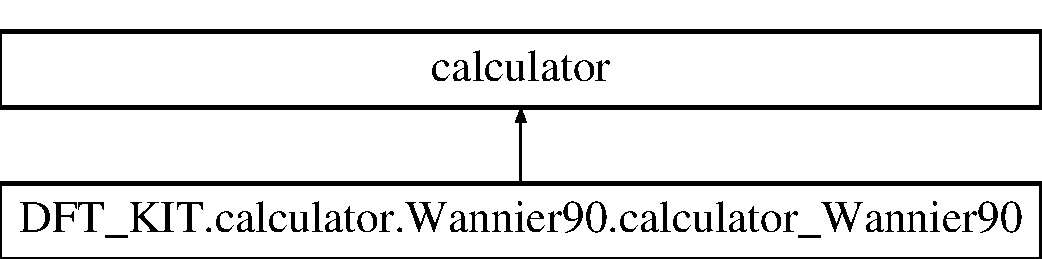
\includegraphics[height=2.000000cm]{class_d_f_t___k_i_t_1_1calculator_1_1_wannier90_1_1calculator___wannier90}
\end{center}
\end{figure}
\subsection*{Public Member Functions}
\begin{DoxyCompactItemize}
\item 
def \hyperlink{class_d_f_t___k_i_t_1_1calculator_1_1_wannier90_1_1calculator___wannier90_a74a7bbb9cae9f82ecbca0cc40980d10e}{\+\_\+\+\_\+init\+\_\+\+\_\+}
\item 
def \hyperlink{class_d_f_t___k_i_t_1_1calculator_1_1_wannier90_1_1calculator___wannier90_a7b4a65524bb0a912f03d3fdbe9813bf7}{add\+\_\+projection}
\item 
def \hyperlink{class_d_f_t___k_i_t_1_1calculator_1_1_wannier90_1_1calculator___wannier90_a16a225c3f0ebca12e4bb8299321d425a}{apply\+\_\+scheme}
\item 
def \hyperlink{class_d_f_t___k_i_t_1_1calculator_1_1_wannier90_1_1calculator___wannier90_aaff180b1ad9f56ce24d2063931eabcc2}{run\+\_\+main}
\item 
def \hyperlink{class_d_f_t___k_i_t_1_1calculator_1_1_wannier90_1_1calculator___wannier90_a8a6d0629564467fa5595aa75a9857bbd}{generate\+\_\+files}
\item 
def \hyperlink{class_d_f_t___k_i_t_1_1calculator_1_1_wannier90_1_1calculator___wannier90_af791da89001cc173855be20c09097166}{run\+\_\+wannier}
\item 
def \hyperlink{class_d_f_t___k_i_t_1_1calculator_1_1_wannier90_1_1calculator___wannier90_a3015ae1b54f5fb07f10d4574f2a528db}{read\+\_\+hamiltonian}
\end{DoxyCompactItemize}
\subsection*{Public Attributes}
\begin{DoxyCompactItemize}
\item 
\hyperlink{class_d_f_t___k_i_t_1_1calculator_1_1_wannier90_1_1calculator___wannier90_a673a29eac1991c2660c4ddf30331d453}{projections}
\end{DoxyCompactItemize}


\subsection{Detailed Description}


Definition at line 32 of file Wannier90.\+py.



\subsection{Constructor \& Destructor Documentation}
\hypertarget{class_d_f_t___k_i_t_1_1calculator_1_1_wannier90_1_1calculator___wannier90_a74a7bbb9cae9f82ecbca0cc40980d10e}{\index{D\+F\+T\+\_\+\+K\+I\+T\+::calculator\+::\+Wannier90\+::calculator\+\_\+\+Wannier90@{D\+F\+T\+\_\+\+K\+I\+T\+::calculator\+::\+Wannier90\+::calculator\+\_\+\+Wannier90}!\+\_\+\+\_\+init\+\_\+\+\_\+@{\+\_\+\+\_\+init\+\_\+\+\_\+}}
\index{\+\_\+\+\_\+init\+\_\+\+\_\+@{\+\_\+\+\_\+init\+\_\+\+\_\+}!D\+F\+T\+\_\+\+K\+I\+T\+::calculator\+::\+Wannier90\+::calculator\+\_\+\+Wannier90@{D\+F\+T\+\_\+\+K\+I\+T\+::calculator\+::\+Wannier90\+::calculator\+\_\+\+Wannier90}}
\subsubsection[{\+\_\+\+\_\+init\+\_\+\+\_\+}]{\setlength{\rightskip}{0pt plus 5cm}def D\+F\+T\+\_\+\+K\+I\+T.\+calculator.\+Wannier90.\+calculator\+\_\+\+Wannier90.\+\_\+\+\_\+init\+\_\+\+\_\+ (
\begin{DoxyParamCaption}
\item[{}]{self, }
\item[{}]{postprocess, }
\item[{}]{dft\+\_\+job, }
\item[{}]{crystal, }
\item[{}]{kgrid, }
\item[{}]{scheme = {\ttfamily 0}, }
\item[{}]{parms}
\end{DoxyParamCaption}
)}}\label{class_d_f_t___k_i_t_1_1calculator_1_1_wannier90_1_1calculator___wannier90_a74a7bbb9cae9f82ecbca0cc40980d10e}


Definition at line 33 of file Wannier90.\+py.



\subsection{Member Function Documentation}
\hypertarget{class_d_f_t___k_i_t_1_1calculator_1_1_wannier90_1_1calculator___wannier90_a7b4a65524bb0a912f03d3fdbe9813bf7}{\index{D\+F\+T\+\_\+\+K\+I\+T\+::calculator\+::\+Wannier90\+::calculator\+\_\+\+Wannier90@{D\+F\+T\+\_\+\+K\+I\+T\+::calculator\+::\+Wannier90\+::calculator\+\_\+\+Wannier90}!add\+\_\+projection@{add\+\_\+projection}}
\index{add\+\_\+projection@{add\+\_\+projection}!D\+F\+T\+\_\+\+K\+I\+T\+::calculator\+::\+Wannier90\+::calculator\+\_\+\+Wannier90@{D\+F\+T\+\_\+\+K\+I\+T\+::calculator\+::\+Wannier90\+::calculator\+\_\+\+Wannier90}}
\subsubsection[{add\+\_\+projection}]{\setlength{\rightskip}{0pt plus 5cm}def D\+F\+T\+\_\+\+K\+I\+T.\+calculator.\+Wannier90.\+calculator\+\_\+\+Wannier90.\+add\+\_\+projection (
\begin{DoxyParamCaption}
\item[{}]{self, }
\item[{}]{proj}
\end{DoxyParamCaption}
)}}\label{class_d_f_t___k_i_t_1_1calculator_1_1_wannier90_1_1calculator___wannier90_a7b4a65524bb0a912f03d3fdbe9813bf7}


Definition at line 38 of file Wannier90.\+py.

\hypertarget{class_d_f_t___k_i_t_1_1calculator_1_1_wannier90_1_1calculator___wannier90_a16a225c3f0ebca12e4bb8299321d425a}{\index{D\+F\+T\+\_\+\+K\+I\+T\+::calculator\+::\+Wannier90\+::calculator\+\_\+\+Wannier90@{D\+F\+T\+\_\+\+K\+I\+T\+::calculator\+::\+Wannier90\+::calculator\+\_\+\+Wannier90}!apply\+\_\+scheme@{apply\+\_\+scheme}}
\index{apply\+\_\+scheme@{apply\+\_\+scheme}!D\+F\+T\+\_\+\+K\+I\+T\+::calculator\+::\+Wannier90\+::calculator\+\_\+\+Wannier90@{D\+F\+T\+\_\+\+K\+I\+T\+::calculator\+::\+Wannier90\+::calculator\+\_\+\+Wannier90}}
\subsubsection[{apply\+\_\+scheme}]{\setlength{\rightskip}{0pt plus 5cm}def D\+F\+T\+\_\+\+K\+I\+T.\+calculator.\+Wannier90.\+calculator\+\_\+\+Wannier90.\+apply\+\_\+scheme (
\begin{DoxyParamCaption}
\item[{}]{self, }
\item[{}]{scheme}
\end{DoxyParamCaption}
)}}\label{class_d_f_t___k_i_t_1_1calculator_1_1_wannier90_1_1calculator___wannier90_a16a225c3f0ebca12e4bb8299321d425a}


Definition at line 41 of file Wannier90.\+py.

\hypertarget{class_d_f_t___k_i_t_1_1calculator_1_1_wannier90_1_1calculator___wannier90_a8a6d0629564467fa5595aa75a9857bbd}{\index{D\+F\+T\+\_\+\+K\+I\+T\+::calculator\+::\+Wannier90\+::calculator\+\_\+\+Wannier90@{D\+F\+T\+\_\+\+K\+I\+T\+::calculator\+::\+Wannier90\+::calculator\+\_\+\+Wannier90}!generate\+\_\+files@{generate\+\_\+files}}
\index{generate\+\_\+files@{generate\+\_\+files}!D\+F\+T\+\_\+\+K\+I\+T\+::calculator\+::\+Wannier90\+::calculator\+\_\+\+Wannier90@{D\+F\+T\+\_\+\+K\+I\+T\+::calculator\+::\+Wannier90\+::calculator\+\_\+\+Wannier90}}
\subsubsection[{generate\+\_\+files}]{\setlength{\rightskip}{0pt plus 5cm}def D\+F\+T\+\_\+\+K\+I\+T.\+calculator.\+Wannier90.\+calculator\+\_\+\+Wannier90.\+generate\+\_\+files (
\begin{DoxyParamCaption}
\item[{}]{self}
\end{DoxyParamCaption}
)}}\label{class_d_f_t___k_i_t_1_1calculator_1_1_wannier90_1_1calculator___wannier90_a8a6d0629564467fa5595aa75a9857bbd}


Definition at line 52 of file Wannier90.\+py.

\hypertarget{class_d_f_t___k_i_t_1_1calculator_1_1_wannier90_1_1calculator___wannier90_a3015ae1b54f5fb07f10d4574f2a528db}{\index{D\+F\+T\+\_\+\+K\+I\+T\+::calculator\+::\+Wannier90\+::calculator\+\_\+\+Wannier90@{D\+F\+T\+\_\+\+K\+I\+T\+::calculator\+::\+Wannier90\+::calculator\+\_\+\+Wannier90}!read\+\_\+hamiltonian@{read\+\_\+hamiltonian}}
\index{read\+\_\+hamiltonian@{read\+\_\+hamiltonian}!D\+F\+T\+\_\+\+K\+I\+T\+::calculator\+::\+Wannier90\+::calculator\+\_\+\+Wannier90@{D\+F\+T\+\_\+\+K\+I\+T\+::calculator\+::\+Wannier90\+::calculator\+\_\+\+Wannier90}}
\subsubsection[{read\+\_\+hamiltonian}]{\setlength{\rightskip}{0pt plus 5cm}def D\+F\+T\+\_\+\+K\+I\+T.\+calculator.\+Wannier90.\+calculator\+\_\+\+Wannier90.\+read\+\_\+hamiltonian (
\begin{DoxyParamCaption}
\item[{}]{self}
\end{DoxyParamCaption}
)}}\label{class_d_f_t___k_i_t_1_1calculator_1_1_wannier90_1_1calculator___wannier90_a3015ae1b54f5fb07f10d4574f2a528db}


Definition at line 91 of file Wannier90.\+py.

\hypertarget{class_d_f_t___k_i_t_1_1calculator_1_1_wannier90_1_1calculator___wannier90_aaff180b1ad9f56ce24d2063931eabcc2}{\index{D\+F\+T\+\_\+\+K\+I\+T\+::calculator\+::\+Wannier90\+::calculator\+\_\+\+Wannier90@{D\+F\+T\+\_\+\+K\+I\+T\+::calculator\+::\+Wannier90\+::calculator\+\_\+\+Wannier90}!run\+\_\+main@{run\+\_\+main}}
\index{run\+\_\+main@{run\+\_\+main}!D\+F\+T\+\_\+\+K\+I\+T\+::calculator\+::\+Wannier90\+::calculator\+\_\+\+Wannier90@{D\+F\+T\+\_\+\+K\+I\+T\+::calculator\+::\+Wannier90\+::calculator\+\_\+\+Wannier90}}
\subsubsection[{run\+\_\+main}]{\setlength{\rightskip}{0pt plus 5cm}def D\+F\+T\+\_\+\+K\+I\+T.\+calculator.\+Wannier90.\+calculator\+\_\+\+Wannier90.\+run\+\_\+main (
\begin{DoxyParamCaption}
\item[{}]{self}
\end{DoxyParamCaption}
)}}\label{class_d_f_t___k_i_t_1_1calculator_1_1_wannier90_1_1calculator___wannier90_aaff180b1ad9f56ce24d2063931eabcc2}


Definition at line 50 of file Wannier90.\+py.

\hypertarget{class_d_f_t___k_i_t_1_1calculator_1_1_wannier90_1_1calculator___wannier90_af791da89001cc173855be20c09097166}{\index{D\+F\+T\+\_\+\+K\+I\+T\+::calculator\+::\+Wannier90\+::calculator\+\_\+\+Wannier90@{D\+F\+T\+\_\+\+K\+I\+T\+::calculator\+::\+Wannier90\+::calculator\+\_\+\+Wannier90}!run\+\_\+wannier@{run\+\_\+wannier}}
\index{run\+\_\+wannier@{run\+\_\+wannier}!D\+F\+T\+\_\+\+K\+I\+T\+::calculator\+::\+Wannier90\+::calculator\+\_\+\+Wannier90@{D\+F\+T\+\_\+\+K\+I\+T\+::calculator\+::\+Wannier90\+::calculator\+\_\+\+Wannier90}}
\subsubsection[{run\+\_\+wannier}]{\setlength{\rightskip}{0pt plus 5cm}def D\+F\+T\+\_\+\+K\+I\+T.\+calculator.\+Wannier90.\+calculator\+\_\+\+Wannier90.\+run\+\_\+wannier (
\begin{DoxyParamCaption}
\item[{}]{self}
\end{DoxyParamCaption}
)}}\label{class_d_f_t___k_i_t_1_1calculator_1_1_wannier90_1_1calculator___wannier90_af791da89001cc173855be20c09097166}


Definition at line 88 of file Wannier90.\+py.



\subsection{Member Data Documentation}
\hypertarget{class_d_f_t___k_i_t_1_1calculator_1_1_wannier90_1_1calculator___wannier90_a673a29eac1991c2660c4ddf30331d453}{\index{D\+F\+T\+\_\+\+K\+I\+T\+::calculator\+::\+Wannier90\+::calculator\+\_\+\+Wannier90@{D\+F\+T\+\_\+\+K\+I\+T\+::calculator\+::\+Wannier90\+::calculator\+\_\+\+Wannier90}!projections@{projections}}
\index{projections@{projections}!D\+F\+T\+\_\+\+K\+I\+T\+::calculator\+::\+Wannier90\+::calculator\+\_\+\+Wannier90@{D\+F\+T\+\_\+\+K\+I\+T\+::calculator\+::\+Wannier90\+::calculator\+\_\+\+Wannier90}}
\subsubsection[{projections}]{\setlength{\rightskip}{0pt plus 5cm}D\+F\+T\+\_\+\+K\+I\+T.\+calculator.\+Wannier90.\+calculator\+\_\+\+Wannier90.\+projections}}\label{class_d_f_t___k_i_t_1_1calculator_1_1_wannier90_1_1calculator___wannier90_a673a29eac1991c2660c4ddf30331d453}


Definition at line 36 of file Wannier90.\+py.



The documentation for this class was generated from the following file\+:\begin{DoxyCompactItemize}
\item 
calculator/\hyperlink{_wannier90_8py}{Wannier90.\+py}\end{DoxyCompactItemize}

\hypertarget{class_d_f_t___k_i_t_1_1core_1_1crystal__3_d_1_1crystal__3_d}{\section{D\+F\+T\+\_\+\+K\+I\+T.\+core.\+crystal\+\_\+3\+D.\+crystal\+\_\+3\+D Class Reference}
\label{class_d_f_t___k_i_t_1_1core_1_1crystal__3_d_1_1crystal__3_d}\index{D\+F\+T\+\_\+\+K\+I\+T.\+core.\+crystal\+\_\+3\+D.\+crystal\+\_\+3\+D@{D\+F\+T\+\_\+\+K\+I\+T.\+core.\+crystal\+\_\+3\+D.\+crystal\+\_\+3\+D}}
}


Class for \hyperlink{class_d_f_t___k_i_t_1_1core_1_1crystal__3_d_1_1crystal__3_d}{crystal\+\_\+3\+D}.  


Inheritance diagram for D\+F\+T\+\_\+\+K\+I\+T.\+core.\+crystal\+\_\+3\+D.\+crystal\+\_\+3\+D\+:\begin{figure}[H]
\begin{center}
\leavevmode
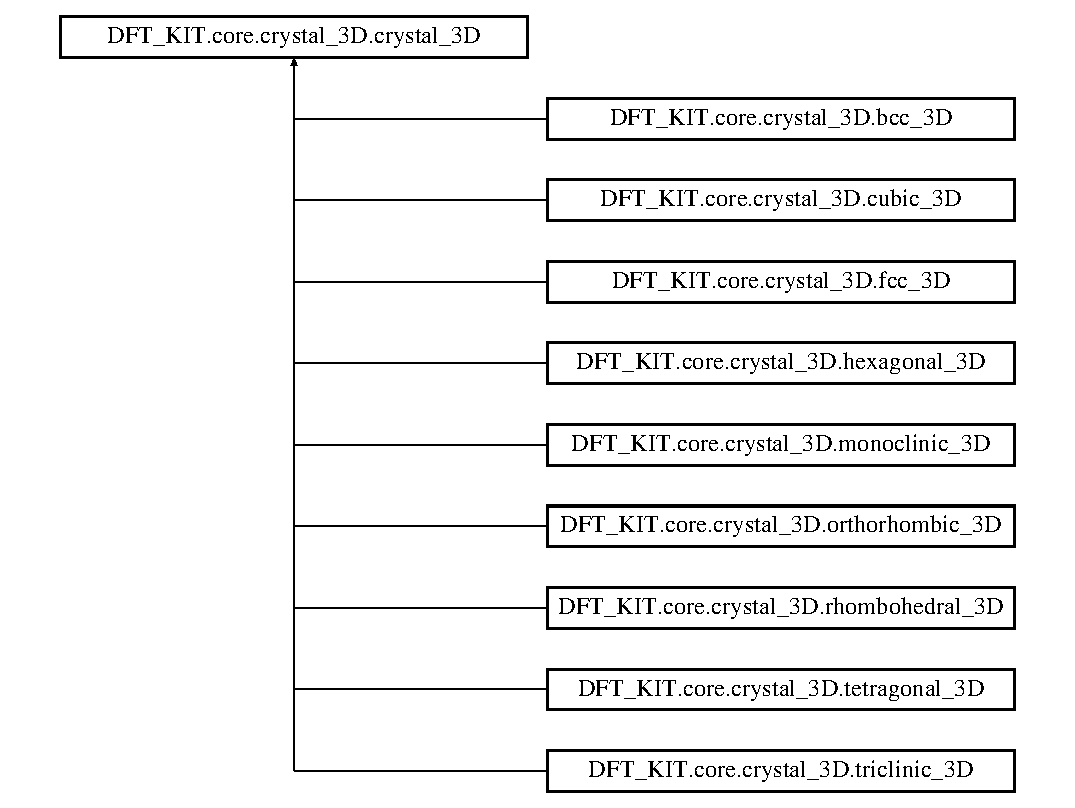
\includegraphics[height=10.000000cm]{class_d_f_t___k_i_t_1_1core_1_1crystal__3_d_1_1crystal__3_d}
\end{center}
\end{figure}
\subsection*{Public Member Functions}
\begin{DoxyCompactItemize}
\item 
def \hyperlink{class_d_f_t___k_i_t_1_1core_1_1crystal__3_d_1_1crystal__3_d_a81cc974b502d653841b6c8a2e8a706e3}{\+\_\+\+\_\+init\+\_\+\+\_\+}
\item 
def \hyperlink{class_d_f_t___k_i_t_1_1core_1_1crystal__3_d_1_1crystal__3_d_a98b65667bfebb65fa63937cc00271445}{set\+\_\+coordinate}
\item 
def \hyperlink{class_d_f_t___k_i_t_1_1core_1_1crystal__3_d_1_1crystal__3_d_a73e3786edda92b516bec8efb8ab051ed}{cart\+\_\+coordinate}
\item 
def \hyperlink{class_d_f_t___k_i_t_1_1core_1_1crystal__3_d_1_1crystal__3_d_aace3722b4eb0d33ecb088dafe8288fe4}{get\+\_\+length\+\_\+unit}
\item 
def \hyperlink{class_d_f_t___k_i_t_1_1core_1_1crystal__3_d_1_1crystal__3_d_a4ba281f8df455078e7f84431d3ffdb24}{set\+\_\+length\+\_\+units}
\item 
def \hyperlink{class_d_f_t___k_i_t_1_1core_1_1crystal__3_d_1_1crystal__3_d_a7d54d2c4a1db3a4698313981eaf665f9}{evaluate\+\_\+basic}
\item 
def \hyperlink{class_d_f_t___k_i_t_1_1core_1_1crystal__3_d_1_1crystal__3_d_aed9febda8b457af38f3d67be521677da}{evaluate\+\_\+rec\+\_\+vectors}
\item 
def \hyperlink{class_d_f_t___k_i_t_1_1core_1_1crystal__3_d_1_1crystal__3_d_a46aa0b8ae019c94ee641bf35a3cd5982}{eval\+\_\+inv\+\_\+primitive\+\_\+vec}
\item 
def \hyperlink{class_d_f_t___k_i_t_1_1core_1_1crystal__3_d_1_1crystal__3_d_abac691db843d918520d382d83bc27204}{eval\+\_\+inv\+\_\+reciprocal\+\_\+vec}
\item 
def \hyperlink{class_d_f_t___k_i_t_1_1core_1_1crystal__3_d_1_1crystal__3_d_aadaa099888d5a26808c88c80f5a4d7ce}{prim\+\_\+to\+\_\+cart}
\item 
def \hyperlink{class_d_f_t___k_i_t_1_1core_1_1crystal__3_d_1_1crystal__3_d_a67a24533e75bbbb543102b71c743057f}{cart\+\_\+to\+\_\+prim}
\item 
def \hyperlink{class_d_f_t___k_i_t_1_1core_1_1crystal__3_d_1_1crystal__3_d_a29201d84a44376c8341bacda16a2d1fd}{get\+\_\+prim\+\_\+vec}
\item 
def \hyperlink{class_d_f_t___k_i_t_1_1core_1_1crystal__3_d_1_1crystal__3_d_ae0a4d3b701cbfd7284596b8ae8eb0739}{set\+\_\+prim\+\_\+vec}
\item 
def \hyperlink{class_d_f_t___k_i_t_1_1core_1_1crystal__3_d_1_1crystal__3_d_a6735ef6cf812229b2c593548ce1447de}{rec\+\_\+to\+\_\+cart}
\item 
def \hyperlink{class_d_f_t___k_i_t_1_1core_1_1crystal__3_d_1_1crystal__3_d_a721a98defd80a609733975ed48cbea9f}{cart\+\_\+to\+\_\+rec}
\item 
def \hyperlink{class_d_f_t___k_i_t_1_1core_1_1crystal__3_d_1_1crystal__3_d_a1f76b8617eb4103847bb6222d945c4f8}{set\+\_\+rec\+\_\+vec}
\item 
def \hyperlink{class_d_f_t___k_i_t_1_1core_1_1crystal__3_d_1_1crystal__3_d_aa08ce34fc1751387bf14569a54ef1011}{get\+\_\+rec\+\_\+vec}
\item 
def \hyperlink{class_d_f_t___k_i_t_1_1core_1_1crystal__3_d_1_1crystal__3_d_ad1f8f615253ba194142c2f59cb776896}{k\+\_\+distance}
\item 
def \hyperlink{class_d_f_t___k_i_t_1_1core_1_1crystal__3_d_1_1crystal__3_d_aa0b95d6d0cd16e2abd5abdbc1c434d86}{special\+\_\+kpoints}
\item 
def \hyperlink{class_d_f_t___k_i_t_1_1core_1_1crystal__3_d_1_1crystal__3_d_ae29abd64a355269fd69a07fb6ed9ec60}{clear\+\_\+klabels}
\item 
def \hyperlink{class_d_f_t___k_i_t_1_1core_1_1crystal__3_d_1_1crystal__3_d_aea6428f48a90700b03e80ce1f9fbab8c}{get\+\_\+num\+\_\+atoms}
\item 
def \hyperlink{class_d_f_t___k_i_t_1_1core_1_1crystal__3_d_1_1crystal__3_d_a2defe3bb26cae50d9e2db2aa6ecb8c24}{get\+\_\+totnum\+\_\+atoms}
\item 
def \hyperlink{class_d_f_t___k_i_t_1_1core_1_1crystal__3_d_1_1crystal__3_d_acd2c68e38e332e0bfc991ae9afc7dd47}{get\+\_\+atom}
\item 
def \hyperlink{class_d_f_t___k_i_t_1_1core_1_1crystal__3_d_1_1crystal__3_d_a357ae4cd95b5bda6efba6c9a0a682a2c}{get\+\_\+atoms\+\_\+groups}
\item 
def \hyperlink{class_d_f_t___k_i_t_1_1core_1_1crystal__3_d_1_1crystal__3_d_acb1087a40c3f003bc9f0f9a0b0b01ec0}{get\+\_\+atoms\+\_\+group}
\item 
def \hyperlink{class_d_f_t___k_i_t_1_1core_1_1crystal__3_d_1_1crystal__3_d_af25d60e4b86b4e5cc4a6f6cdcebc0d9a}{add\+\_\+atom}
\item 
def \hyperlink{class_d_f_t___k_i_t_1_1core_1_1crystal__3_d_1_1crystal__3_d_a9b4a68b6f60f06fc64184a0aaa7e1ef5}{add\+\_\+atoms}
\item 
def \hyperlink{class_d_f_t___k_i_t_1_1core_1_1crystal__3_d_1_1crystal__3_d_a16ec5e68e37cf1ceca5a95c7e6574f71}{updata\+\_\+position}
\end{DoxyCompactItemize}
\subsection*{Public Attributes}
\begin{DoxyCompactItemize}
\item 
\hyperlink{class_d_f_t___k_i_t_1_1core_1_1crystal__3_d_1_1crystal__3_d_a0239fc0cee6cd4e79ce9d7175ceb585d}{description}
\item 
\hyperlink{class_d_f_t___k_i_t_1_1core_1_1crystal__3_d_1_1crystal__3_d_a8be1646b7a612989dc73502430a450c2}{primitive\+\_\+vector}
\item 
\hyperlink{class_d_f_t___k_i_t_1_1core_1_1crystal__3_d_1_1crystal__3_d_a8da908b53e91c839cab9e0efe07cc3fd}{inv\+\_\+primitive\+\_\+vector}
\item 
\hyperlink{class_d_f_t___k_i_t_1_1core_1_1crystal__3_d_1_1crystal__3_d_ac792f9a47ced7b38b07d17d55e043d3b}{reciprocal\+\_\+vector}
\item 
\hyperlink{class_d_f_t___k_i_t_1_1core_1_1crystal__3_d_1_1crystal__3_d_a7d30d0f0c094774e655b37eb1e957a03}{inv\+\_\+reciprocal\+\_\+vector}
\item 
\hyperlink{class_d_f_t___k_i_t_1_1core_1_1crystal__3_d_1_1crystal__3_d_a5e317e2491734325c03e50c6f3823d45}{length\+\_\+unit}
\item 
\hyperlink{class_d_f_t___k_i_t_1_1core_1_1crystal__3_d_1_1crystal__3_d_ab74777e35fe1ceb493515252c4e11b07}{basis\+\_\+atom\+\_\+groups}
\item 
\hyperlink{class_d_f_t___k_i_t_1_1core_1_1crystal__3_d_1_1crystal__3_d_af70e4b25b18a6ec1868c2e6e445dbb13}{basis\+\_\+element}
\item 
\hyperlink{class_d_f_t___k_i_t_1_1core_1_1crystal__3_d_1_1crystal__3_d_acdab713c57aa03bb2b557943925ee427}{k\+\_\+labels}
\item 
\hyperlink{class_d_f_t___k_i_t_1_1core_1_1crystal__3_d_1_1crystal__3_d_a03d6814d7345e080c021bbadc0b60ba7}{k\+\_\+directions}
\item 
\hyperlink{class_d_f_t___k_i_t_1_1core_1_1crystal__3_d_1_1crystal__3_d_acb068ebdcded14e39fba88ab7699fe4a}{cart\+\_\+coordinate}
\item 
\hyperlink{class_d_f_t___k_i_t_1_1core_1_1crystal__3_d_1_1crystal__3_d_a33bce31d085891baa0a4b7836d255980}{length\+\_\+units}
\end{DoxyCompactItemize}


\subsection{Detailed Description}
Class for \hyperlink{class_d_f_t___k_i_t_1_1core_1_1crystal__3_d_1_1crystal__3_d}{crystal\+\_\+3\+D}. 


\begin{DoxyParams}{Parameters}
{\em length\+\_\+unit} & define the length\+\_\+unit in the calculation (1 angstrom) \\
\hline
\end{DoxyParams}


Definition at line 17 of file crystal\+\_\+3\+D.\+py.



\subsection{Constructor \& Destructor Documentation}
\hypertarget{class_d_f_t___k_i_t_1_1core_1_1crystal__3_d_1_1crystal__3_d_a81cc974b502d653841b6c8a2e8a706e3}{\index{D\+F\+T\+\_\+\+K\+I\+T\+::core\+::crystal\+\_\+3\+D\+::crystal\+\_\+3\+D@{D\+F\+T\+\_\+\+K\+I\+T\+::core\+::crystal\+\_\+3\+D\+::crystal\+\_\+3\+D}!\+\_\+\+\_\+init\+\_\+\+\_\+@{\+\_\+\+\_\+init\+\_\+\+\_\+}}
\index{\+\_\+\+\_\+init\+\_\+\+\_\+@{\+\_\+\+\_\+init\+\_\+\+\_\+}!D\+F\+T\+\_\+\+K\+I\+T\+::core\+::crystal\+\_\+3\+D\+::crystal\+\_\+3\+D@{D\+F\+T\+\_\+\+K\+I\+T\+::core\+::crystal\+\_\+3\+D\+::crystal\+\_\+3\+D}}
\subsubsection[{\+\_\+\+\_\+init\+\_\+\+\_\+}]{\setlength{\rightskip}{0pt plus 5cm}def D\+F\+T\+\_\+\+K\+I\+T.\+core.\+crystal\+\_\+3\+D.\+crystal\+\_\+3\+D.\+\_\+\+\_\+init\+\_\+\+\_\+ (
\begin{DoxyParamCaption}
\item[{}]{self, }
\item[{}]{length\+\_\+unit = {\ttfamily 1.0}, }
\item[{}]{description = {\ttfamily 'CRYSTAL~generated~by~DFT\+\_\+KIT'}}
\end{DoxyParamCaption}
)}}\label{class_d_f_t___k_i_t_1_1core_1_1crystal__3_d_1_1crystal__3_d_a81cc974b502d653841b6c8a2e8a706e3}


Definition at line 18 of file crystal\+\_\+3\+D.\+py.



\subsection{Member Function Documentation}
\hypertarget{class_d_f_t___k_i_t_1_1core_1_1crystal__3_d_1_1crystal__3_d_af25d60e4b86b4e5cc4a6f6cdcebc0d9a}{\index{D\+F\+T\+\_\+\+K\+I\+T\+::core\+::crystal\+\_\+3\+D\+::crystal\+\_\+3\+D@{D\+F\+T\+\_\+\+K\+I\+T\+::core\+::crystal\+\_\+3\+D\+::crystal\+\_\+3\+D}!add\+\_\+atom@{add\+\_\+atom}}
\index{add\+\_\+atom@{add\+\_\+atom}!D\+F\+T\+\_\+\+K\+I\+T\+::core\+::crystal\+\_\+3\+D\+::crystal\+\_\+3\+D@{D\+F\+T\+\_\+\+K\+I\+T\+::core\+::crystal\+\_\+3\+D\+::crystal\+\_\+3\+D}}
\subsubsection[{add\+\_\+atom}]{\setlength{\rightskip}{0pt plus 5cm}def D\+F\+T\+\_\+\+K\+I\+T.\+core.\+crystal\+\_\+3\+D.\+crystal\+\_\+3\+D.\+add\+\_\+atom (
\begin{DoxyParamCaption}
\item[{}]{self, }
\item[{}]{element, }
\item[{}]{position = {\ttfamily np.array(\mbox{[}0.0,0.0}, }
\item[{}]{parms}
\end{DoxyParamCaption}
)}}\label{class_d_f_t___k_i_t_1_1core_1_1crystal__3_d_1_1crystal__3_d_af25d60e4b86b4e5cc4a6f6cdcebc0d9a}


Definition at line 121 of file crystal\+\_\+3\+D.\+py.

\hypertarget{class_d_f_t___k_i_t_1_1core_1_1crystal__3_d_1_1crystal__3_d_a9b4a68b6f60f06fc64184a0aaa7e1ef5}{\index{D\+F\+T\+\_\+\+K\+I\+T\+::core\+::crystal\+\_\+3\+D\+::crystal\+\_\+3\+D@{D\+F\+T\+\_\+\+K\+I\+T\+::core\+::crystal\+\_\+3\+D\+::crystal\+\_\+3\+D}!add\+\_\+atoms@{add\+\_\+atoms}}
\index{add\+\_\+atoms@{add\+\_\+atoms}!D\+F\+T\+\_\+\+K\+I\+T\+::core\+::crystal\+\_\+3\+D\+::crystal\+\_\+3\+D@{D\+F\+T\+\_\+\+K\+I\+T\+::core\+::crystal\+\_\+3\+D\+::crystal\+\_\+3\+D}}
\subsubsection[{add\+\_\+atoms}]{\setlength{\rightskip}{0pt plus 5cm}def D\+F\+T\+\_\+\+K\+I\+T.\+core.\+crystal\+\_\+3\+D.\+crystal\+\_\+3\+D.\+add\+\_\+atoms (
\begin{DoxyParamCaption}
\item[{}]{self, }
\item[{}]{element, }
\item[{}]{positions, }
\item[{}]{parms}
\end{DoxyParamCaption}
)}}\label{class_d_f_t___k_i_t_1_1core_1_1crystal__3_d_1_1crystal__3_d_a9b4a68b6f60f06fc64184a0aaa7e1ef5}


Definition at line 129 of file crystal\+\_\+3\+D.\+py.

\hypertarget{class_d_f_t___k_i_t_1_1core_1_1crystal__3_d_1_1crystal__3_d_a73e3786edda92b516bec8efb8ab051ed}{\index{D\+F\+T\+\_\+\+K\+I\+T\+::core\+::crystal\+\_\+3\+D\+::crystal\+\_\+3\+D@{D\+F\+T\+\_\+\+K\+I\+T\+::core\+::crystal\+\_\+3\+D\+::crystal\+\_\+3\+D}!cart\+\_\+coordinate@{cart\+\_\+coordinate}}
\index{cart\+\_\+coordinate@{cart\+\_\+coordinate}!D\+F\+T\+\_\+\+K\+I\+T\+::core\+::crystal\+\_\+3\+D\+::crystal\+\_\+3\+D@{D\+F\+T\+\_\+\+K\+I\+T\+::core\+::crystal\+\_\+3\+D\+::crystal\+\_\+3\+D}}
\subsubsection[{cart\+\_\+coordinate}]{\setlength{\rightskip}{0pt plus 5cm}def D\+F\+T\+\_\+\+K\+I\+T.\+core.\+crystal\+\_\+3\+D.\+crystal\+\_\+3\+D.\+cart\+\_\+coordinate (
\begin{DoxyParamCaption}
\item[{}]{self}
\end{DoxyParamCaption}
)}}\label{class_d_f_t___k_i_t_1_1core_1_1crystal__3_d_1_1crystal__3_d_a73e3786edda92b516bec8efb8ab051ed}


Definition at line 41 of file crystal\+\_\+3\+D.\+py.

\hypertarget{class_d_f_t___k_i_t_1_1core_1_1crystal__3_d_1_1crystal__3_d_a67a24533e75bbbb543102b71c743057f}{\index{D\+F\+T\+\_\+\+K\+I\+T\+::core\+::crystal\+\_\+3\+D\+::crystal\+\_\+3\+D@{D\+F\+T\+\_\+\+K\+I\+T\+::core\+::crystal\+\_\+3\+D\+::crystal\+\_\+3\+D}!cart\+\_\+to\+\_\+prim@{cart\+\_\+to\+\_\+prim}}
\index{cart\+\_\+to\+\_\+prim@{cart\+\_\+to\+\_\+prim}!D\+F\+T\+\_\+\+K\+I\+T\+::core\+::crystal\+\_\+3\+D\+::crystal\+\_\+3\+D@{D\+F\+T\+\_\+\+K\+I\+T\+::core\+::crystal\+\_\+3\+D\+::crystal\+\_\+3\+D}}
\subsubsection[{cart\+\_\+to\+\_\+prim}]{\setlength{\rightskip}{0pt plus 5cm}def D\+F\+T\+\_\+\+K\+I\+T.\+core.\+crystal\+\_\+3\+D.\+crystal\+\_\+3\+D.\+cart\+\_\+to\+\_\+prim (
\begin{DoxyParamCaption}
\item[{}]{self, }
\item[{}]{vec\+\_\+}
\end{DoxyParamCaption}
)}}\label{class_d_f_t___k_i_t_1_1core_1_1crystal__3_d_1_1crystal__3_d_a67a24533e75bbbb543102b71c743057f}


Definition at line 78 of file crystal\+\_\+3\+D.\+py.

\hypertarget{class_d_f_t___k_i_t_1_1core_1_1crystal__3_d_1_1crystal__3_d_a721a98defd80a609733975ed48cbea9f}{\index{D\+F\+T\+\_\+\+K\+I\+T\+::core\+::crystal\+\_\+3\+D\+::crystal\+\_\+3\+D@{D\+F\+T\+\_\+\+K\+I\+T\+::core\+::crystal\+\_\+3\+D\+::crystal\+\_\+3\+D}!cart\+\_\+to\+\_\+rec@{cart\+\_\+to\+\_\+rec}}
\index{cart\+\_\+to\+\_\+rec@{cart\+\_\+to\+\_\+rec}!D\+F\+T\+\_\+\+K\+I\+T\+::core\+::crystal\+\_\+3\+D\+::crystal\+\_\+3\+D@{D\+F\+T\+\_\+\+K\+I\+T\+::core\+::crystal\+\_\+3\+D\+::crystal\+\_\+3\+D}}
\subsubsection[{cart\+\_\+to\+\_\+rec}]{\setlength{\rightskip}{0pt plus 5cm}def D\+F\+T\+\_\+\+K\+I\+T.\+core.\+crystal\+\_\+3\+D.\+crystal\+\_\+3\+D.\+cart\+\_\+to\+\_\+rec (
\begin{DoxyParamCaption}
\item[{}]{self, }
\item[{}]{vec\+\_\+}
\end{DoxyParamCaption}
)}}\label{class_d_f_t___k_i_t_1_1core_1_1crystal__3_d_1_1crystal__3_d_a721a98defd80a609733975ed48cbea9f}


Definition at line 86 of file crystal\+\_\+3\+D.\+py.

\hypertarget{class_d_f_t___k_i_t_1_1core_1_1crystal__3_d_1_1crystal__3_d_ae29abd64a355269fd69a07fb6ed9ec60}{\index{D\+F\+T\+\_\+\+K\+I\+T\+::core\+::crystal\+\_\+3\+D\+::crystal\+\_\+3\+D@{D\+F\+T\+\_\+\+K\+I\+T\+::core\+::crystal\+\_\+3\+D\+::crystal\+\_\+3\+D}!clear\+\_\+klabels@{clear\+\_\+klabels}}
\index{clear\+\_\+klabels@{clear\+\_\+klabels}!D\+F\+T\+\_\+\+K\+I\+T\+::core\+::crystal\+\_\+3\+D\+::crystal\+\_\+3\+D@{D\+F\+T\+\_\+\+K\+I\+T\+::core\+::crystal\+\_\+3\+D\+::crystal\+\_\+3\+D}}
\subsubsection[{clear\+\_\+klabels}]{\setlength{\rightskip}{0pt plus 5cm}def D\+F\+T\+\_\+\+K\+I\+T.\+core.\+crystal\+\_\+3\+D.\+crystal\+\_\+3\+D.\+clear\+\_\+klabels (
\begin{DoxyParamCaption}
\item[{}]{self}
\end{DoxyParamCaption}
)}}\label{class_d_f_t___k_i_t_1_1core_1_1crystal__3_d_1_1crystal__3_d_ae29abd64a355269fd69a07fb6ed9ec60}


Definition at line 98 of file crystal\+\_\+3\+D.\+py.

\hypertarget{class_d_f_t___k_i_t_1_1core_1_1crystal__3_d_1_1crystal__3_d_a46aa0b8ae019c94ee641bf35a3cd5982}{\index{D\+F\+T\+\_\+\+K\+I\+T\+::core\+::crystal\+\_\+3\+D\+::crystal\+\_\+3\+D@{D\+F\+T\+\_\+\+K\+I\+T\+::core\+::crystal\+\_\+3\+D\+::crystal\+\_\+3\+D}!eval\+\_\+inv\+\_\+primitive\+\_\+vec@{eval\+\_\+inv\+\_\+primitive\+\_\+vec}}
\index{eval\+\_\+inv\+\_\+primitive\+\_\+vec@{eval\+\_\+inv\+\_\+primitive\+\_\+vec}!D\+F\+T\+\_\+\+K\+I\+T\+::core\+::crystal\+\_\+3\+D\+::crystal\+\_\+3\+D@{D\+F\+T\+\_\+\+K\+I\+T\+::core\+::crystal\+\_\+3\+D\+::crystal\+\_\+3\+D}}
\subsubsection[{eval\+\_\+inv\+\_\+primitive\+\_\+vec}]{\setlength{\rightskip}{0pt plus 5cm}def D\+F\+T\+\_\+\+K\+I\+T.\+core.\+crystal\+\_\+3\+D.\+crystal\+\_\+3\+D.\+eval\+\_\+inv\+\_\+primitive\+\_\+vec (
\begin{DoxyParamCaption}
\item[{}]{self}
\end{DoxyParamCaption}
)}}\label{class_d_f_t___k_i_t_1_1core_1_1crystal__3_d_1_1crystal__3_d_a46aa0b8ae019c94ee641bf35a3cd5982}


Definition at line 61 of file crystal\+\_\+3\+D.\+py.

\hypertarget{class_d_f_t___k_i_t_1_1core_1_1crystal__3_d_1_1crystal__3_d_abac691db843d918520d382d83bc27204}{\index{D\+F\+T\+\_\+\+K\+I\+T\+::core\+::crystal\+\_\+3\+D\+::crystal\+\_\+3\+D@{D\+F\+T\+\_\+\+K\+I\+T\+::core\+::crystal\+\_\+3\+D\+::crystal\+\_\+3\+D}!eval\+\_\+inv\+\_\+reciprocal\+\_\+vec@{eval\+\_\+inv\+\_\+reciprocal\+\_\+vec}}
\index{eval\+\_\+inv\+\_\+reciprocal\+\_\+vec@{eval\+\_\+inv\+\_\+reciprocal\+\_\+vec}!D\+F\+T\+\_\+\+K\+I\+T\+::core\+::crystal\+\_\+3\+D\+::crystal\+\_\+3\+D@{D\+F\+T\+\_\+\+K\+I\+T\+::core\+::crystal\+\_\+3\+D\+::crystal\+\_\+3\+D}}
\subsubsection[{eval\+\_\+inv\+\_\+reciprocal\+\_\+vec}]{\setlength{\rightskip}{0pt plus 5cm}def D\+F\+T\+\_\+\+K\+I\+T.\+core.\+crystal\+\_\+3\+D.\+crystal\+\_\+3\+D.\+eval\+\_\+inv\+\_\+reciprocal\+\_\+vec (
\begin{DoxyParamCaption}
\item[{}]{self}
\end{DoxyParamCaption}
)}}\label{class_d_f_t___k_i_t_1_1core_1_1crystal__3_d_1_1crystal__3_d_abac691db843d918520d382d83bc27204}


Definition at line 68 of file crystal\+\_\+3\+D.\+py.

\hypertarget{class_d_f_t___k_i_t_1_1core_1_1crystal__3_d_1_1crystal__3_d_a7d54d2c4a1db3a4698313981eaf665f9}{\index{D\+F\+T\+\_\+\+K\+I\+T\+::core\+::crystal\+\_\+3\+D\+::crystal\+\_\+3\+D@{D\+F\+T\+\_\+\+K\+I\+T\+::core\+::crystal\+\_\+3\+D\+::crystal\+\_\+3\+D}!evaluate\+\_\+basic@{evaluate\+\_\+basic}}
\index{evaluate\+\_\+basic@{evaluate\+\_\+basic}!D\+F\+T\+\_\+\+K\+I\+T\+::core\+::crystal\+\_\+3\+D\+::crystal\+\_\+3\+D@{D\+F\+T\+\_\+\+K\+I\+T\+::core\+::crystal\+\_\+3\+D\+::crystal\+\_\+3\+D}}
\subsubsection[{evaluate\+\_\+basic}]{\setlength{\rightskip}{0pt plus 5cm}def D\+F\+T\+\_\+\+K\+I\+T.\+core.\+crystal\+\_\+3\+D.\+crystal\+\_\+3\+D.\+evaluate\+\_\+basic (
\begin{DoxyParamCaption}
\item[{}]{self}
\end{DoxyParamCaption}
)}}\label{class_d_f_t___k_i_t_1_1core_1_1crystal__3_d_1_1crystal__3_d_a7d54d2c4a1db3a4698313981eaf665f9}


Definition at line 51 of file crystal\+\_\+3\+D.\+py.

\hypertarget{class_d_f_t___k_i_t_1_1core_1_1crystal__3_d_1_1crystal__3_d_aed9febda8b457af38f3d67be521677da}{\index{D\+F\+T\+\_\+\+K\+I\+T\+::core\+::crystal\+\_\+3\+D\+::crystal\+\_\+3\+D@{D\+F\+T\+\_\+\+K\+I\+T\+::core\+::crystal\+\_\+3\+D\+::crystal\+\_\+3\+D}!evaluate\+\_\+rec\+\_\+vectors@{evaluate\+\_\+rec\+\_\+vectors}}
\index{evaluate\+\_\+rec\+\_\+vectors@{evaluate\+\_\+rec\+\_\+vectors}!D\+F\+T\+\_\+\+K\+I\+T\+::core\+::crystal\+\_\+3\+D\+::crystal\+\_\+3\+D@{D\+F\+T\+\_\+\+K\+I\+T\+::core\+::crystal\+\_\+3\+D\+::crystal\+\_\+3\+D}}
\subsubsection[{evaluate\+\_\+rec\+\_\+vectors}]{\setlength{\rightskip}{0pt plus 5cm}def D\+F\+T\+\_\+\+K\+I\+T.\+core.\+crystal\+\_\+3\+D.\+crystal\+\_\+3\+D.\+evaluate\+\_\+rec\+\_\+vectors (
\begin{DoxyParamCaption}
\item[{}]{self}
\end{DoxyParamCaption}
)}}\label{class_d_f_t___k_i_t_1_1core_1_1crystal__3_d_1_1crystal__3_d_aed9febda8b457af38f3d67be521677da}


Definition at line 56 of file crystal\+\_\+3\+D.\+py.

\hypertarget{class_d_f_t___k_i_t_1_1core_1_1crystal__3_d_1_1crystal__3_d_acd2c68e38e332e0bfc991ae9afc7dd47}{\index{D\+F\+T\+\_\+\+K\+I\+T\+::core\+::crystal\+\_\+3\+D\+::crystal\+\_\+3\+D@{D\+F\+T\+\_\+\+K\+I\+T\+::core\+::crystal\+\_\+3\+D\+::crystal\+\_\+3\+D}!get\+\_\+atom@{get\+\_\+atom}}
\index{get\+\_\+atom@{get\+\_\+atom}!D\+F\+T\+\_\+\+K\+I\+T\+::core\+::crystal\+\_\+3\+D\+::crystal\+\_\+3\+D@{D\+F\+T\+\_\+\+K\+I\+T\+::core\+::crystal\+\_\+3\+D\+::crystal\+\_\+3\+D}}
\subsubsection[{get\+\_\+atom}]{\setlength{\rightskip}{0pt plus 5cm}def D\+F\+T\+\_\+\+K\+I\+T.\+core.\+crystal\+\_\+3\+D.\+crystal\+\_\+3\+D.\+get\+\_\+atom (
\begin{DoxyParamCaption}
\item[{}]{self, }
\item[{}]{group, }
\item[{}]{num}
\end{DoxyParamCaption}
)}}\label{class_d_f_t___k_i_t_1_1core_1_1crystal__3_d_1_1crystal__3_d_acd2c68e38e332e0bfc991ae9afc7dd47}


Definition at line 114 of file crystal\+\_\+3\+D.\+py.

\hypertarget{class_d_f_t___k_i_t_1_1core_1_1crystal__3_d_1_1crystal__3_d_acb1087a40c3f003bc9f0f9a0b0b01ec0}{\index{D\+F\+T\+\_\+\+K\+I\+T\+::core\+::crystal\+\_\+3\+D\+::crystal\+\_\+3\+D@{D\+F\+T\+\_\+\+K\+I\+T\+::core\+::crystal\+\_\+3\+D\+::crystal\+\_\+3\+D}!get\+\_\+atoms\+\_\+group@{get\+\_\+atoms\+\_\+group}}
\index{get\+\_\+atoms\+\_\+group@{get\+\_\+atoms\+\_\+group}!D\+F\+T\+\_\+\+K\+I\+T\+::core\+::crystal\+\_\+3\+D\+::crystal\+\_\+3\+D@{D\+F\+T\+\_\+\+K\+I\+T\+::core\+::crystal\+\_\+3\+D\+::crystal\+\_\+3\+D}}
\subsubsection[{get\+\_\+atoms\+\_\+group}]{\setlength{\rightskip}{0pt plus 5cm}def D\+F\+T\+\_\+\+K\+I\+T.\+core.\+crystal\+\_\+3\+D.\+crystal\+\_\+3\+D.\+get\+\_\+atoms\+\_\+group (
\begin{DoxyParamCaption}
\item[{}]{self, }
\item[{}]{group}
\end{DoxyParamCaption}
)}}\label{class_d_f_t___k_i_t_1_1core_1_1crystal__3_d_1_1crystal__3_d_acb1087a40c3f003bc9f0f9a0b0b01ec0}


Definition at line 118 of file crystal\+\_\+3\+D.\+py.

\hypertarget{class_d_f_t___k_i_t_1_1core_1_1crystal__3_d_1_1crystal__3_d_a357ae4cd95b5bda6efba6c9a0a682a2c}{\index{D\+F\+T\+\_\+\+K\+I\+T\+::core\+::crystal\+\_\+3\+D\+::crystal\+\_\+3\+D@{D\+F\+T\+\_\+\+K\+I\+T\+::core\+::crystal\+\_\+3\+D\+::crystal\+\_\+3\+D}!get\+\_\+atoms\+\_\+groups@{get\+\_\+atoms\+\_\+groups}}
\index{get\+\_\+atoms\+\_\+groups@{get\+\_\+atoms\+\_\+groups}!D\+F\+T\+\_\+\+K\+I\+T\+::core\+::crystal\+\_\+3\+D\+::crystal\+\_\+3\+D@{D\+F\+T\+\_\+\+K\+I\+T\+::core\+::crystal\+\_\+3\+D\+::crystal\+\_\+3\+D}}
\subsubsection[{get\+\_\+atoms\+\_\+groups}]{\setlength{\rightskip}{0pt plus 5cm}def D\+F\+T\+\_\+\+K\+I\+T.\+core.\+crystal\+\_\+3\+D.\+crystal\+\_\+3\+D.\+get\+\_\+atoms\+\_\+groups (
\begin{DoxyParamCaption}
\item[{}]{self}
\end{DoxyParamCaption}
)}}\label{class_d_f_t___k_i_t_1_1core_1_1crystal__3_d_1_1crystal__3_d_a357ae4cd95b5bda6efba6c9a0a682a2c}


Definition at line 116 of file crystal\+\_\+3\+D.\+py.

\hypertarget{class_d_f_t___k_i_t_1_1core_1_1crystal__3_d_1_1crystal__3_d_aace3722b4eb0d33ecb088dafe8288fe4}{\index{D\+F\+T\+\_\+\+K\+I\+T\+::core\+::crystal\+\_\+3\+D\+::crystal\+\_\+3\+D@{D\+F\+T\+\_\+\+K\+I\+T\+::core\+::crystal\+\_\+3\+D\+::crystal\+\_\+3\+D}!get\+\_\+length\+\_\+unit@{get\+\_\+length\+\_\+unit}}
\index{get\+\_\+length\+\_\+unit@{get\+\_\+length\+\_\+unit}!D\+F\+T\+\_\+\+K\+I\+T\+::core\+::crystal\+\_\+3\+D\+::crystal\+\_\+3\+D@{D\+F\+T\+\_\+\+K\+I\+T\+::core\+::crystal\+\_\+3\+D\+::crystal\+\_\+3\+D}}
\subsubsection[{get\+\_\+length\+\_\+unit}]{\setlength{\rightskip}{0pt plus 5cm}def D\+F\+T\+\_\+\+K\+I\+T.\+core.\+crystal\+\_\+3\+D.\+crystal\+\_\+3\+D.\+get\+\_\+length\+\_\+unit (
\begin{DoxyParamCaption}
\item[{}]{self}
\end{DoxyParamCaption}
)}}\label{class_d_f_t___k_i_t_1_1core_1_1crystal__3_d_1_1crystal__3_d_aace3722b4eb0d33ecb088dafe8288fe4}


Definition at line 44 of file crystal\+\_\+3\+D.\+py.

\hypertarget{class_d_f_t___k_i_t_1_1core_1_1crystal__3_d_1_1crystal__3_d_aea6428f48a90700b03e80ce1f9fbab8c}{\index{D\+F\+T\+\_\+\+K\+I\+T\+::core\+::crystal\+\_\+3\+D\+::crystal\+\_\+3\+D@{D\+F\+T\+\_\+\+K\+I\+T\+::core\+::crystal\+\_\+3\+D\+::crystal\+\_\+3\+D}!get\+\_\+num\+\_\+atoms@{get\+\_\+num\+\_\+atoms}}
\index{get\+\_\+num\+\_\+atoms@{get\+\_\+num\+\_\+atoms}!D\+F\+T\+\_\+\+K\+I\+T\+::core\+::crystal\+\_\+3\+D\+::crystal\+\_\+3\+D@{D\+F\+T\+\_\+\+K\+I\+T\+::core\+::crystal\+\_\+3\+D\+::crystal\+\_\+3\+D}}
\subsubsection[{get\+\_\+num\+\_\+atoms}]{\setlength{\rightskip}{0pt plus 5cm}def D\+F\+T\+\_\+\+K\+I\+T.\+core.\+crystal\+\_\+3\+D.\+crystal\+\_\+3\+D.\+get\+\_\+num\+\_\+atoms (
\begin{DoxyParamCaption}
\item[{}]{self, }
\item[{}]{group}
\end{DoxyParamCaption}
)}}\label{class_d_f_t___k_i_t_1_1core_1_1crystal__3_d_1_1crystal__3_d_aea6428f48a90700b03e80ce1f9fbab8c}


Definition at line 103 of file crystal\+\_\+3\+D.\+py.

\hypertarget{class_d_f_t___k_i_t_1_1core_1_1crystal__3_d_1_1crystal__3_d_a29201d84a44376c8341bacda16a2d1fd}{\index{D\+F\+T\+\_\+\+K\+I\+T\+::core\+::crystal\+\_\+3\+D\+::crystal\+\_\+3\+D@{D\+F\+T\+\_\+\+K\+I\+T\+::core\+::crystal\+\_\+3\+D\+::crystal\+\_\+3\+D}!get\+\_\+prim\+\_\+vec@{get\+\_\+prim\+\_\+vec}}
\index{get\+\_\+prim\+\_\+vec@{get\+\_\+prim\+\_\+vec}!D\+F\+T\+\_\+\+K\+I\+T\+::core\+::crystal\+\_\+3\+D\+::crystal\+\_\+3\+D@{D\+F\+T\+\_\+\+K\+I\+T\+::core\+::crystal\+\_\+3\+D\+::crystal\+\_\+3\+D}}
\subsubsection[{get\+\_\+prim\+\_\+vec}]{\setlength{\rightskip}{0pt plus 5cm}def D\+F\+T\+\_\+\+K\+I\+T.\+core.\+crystal\+\_\+3\+D.\+crystal\+\_\+3\+D.\+get\+\_\+prim\+\_\+vec (
\begin{DoxyParamCaption}
\item[{}]{self, }
\item[{}]{num\+\_\+}
\end{DoxyParamCaption}
)}}\label{class_d_f_t___k_i_t_1_1core_1_1crystal__3_d_1_1crystal__3_d_a29201d84a44376c8341bacda16a2d1fd}


Definition at line 80 of file crystal\+\_\+3\+D.\+py.

\hypertarget{class_d_f_t___k_i_t_1_1core_1_1crystal__3_d_1_1crystal__3_d_aa08ce34fc1751387bf14569a54ef1011}{\index{D\+F\+T\+\_\+\+K\+I\+T\+::core\+::crystal\+\_\+3\+D\+::crystal\+\_\+3\+D@{D\+F\+T\+\_\+\+K\+I\+T\+::core\+::crystal\+\_\+3\+D\+::crystal\+\_\+3\+D}!get\+\_\+rec\+\_\+vec@{get\+\_\+rec\+\_\+vec}}
\index{get\+\_\+rec\+\_\+vec@{get\+\_\+rec\+\_\+vec}!D\+F\+T\+\_\+\+K\+I\+T\+::core\+::crystal\+\_\+3\+D\+::crystal\+\_\+3\+D@{D\+F\+T\+\_\+\+K\+I\+T\+::core\+::crystal\+\_\+3\+D\+::crystal\+\_\+3\+D}}
\subsubsection[{get\+\_\+rec\+\_\+vec}]{\setlength{\rightskip}{0pt plus 5cm}def D\+F\+T\+\_\+\+K\+I\+T.\+core.\+crystal\+\_\+3\+D.\+crystal\+\_\+3\+D.\+get\+\_\+rec\+\_\+vec (
\begin{DoxyParamCaption}
\item[{}]{self, }
\item[{}]{vec\+\_\+num}
\end{DoxyParamCaption}
)}}\label{class_d_f_t___k_i_t_1_1core_1_1crystal__3_d_1_1crystal__3_d_aa08ce34fc1751387bf14569a54ef1011}


Definition at line 90 of file crystal\+\_\+3\+D.\+py.

\hypertarget{class_d_f_t___k_i_t_1_1core_1_1crystal__3_d_1_1crystal__3_d_a2defe3bb26cae50d9e2db2aa6ecb8c24}{\index{D\+F\+T\+\_\+\+K\+I\+T\+::core\+::crystal\+\_\+3\+D\+::crystal\+\_\+3\+D@{D\+F\+T\+\_\+\+K\+I\+T\+::core\+::crystal\+\_\+3\+D\+::crystal\+\_\+3\+D}!get\+\_\+totnum\+\_\+atoms@{get\+\_\+totnum\+\_\+atoms}}
\index{get\+\_\+totnum\+\_\+atoms@{get\+\_\+totnum\+\_\+atoms}!D\+F\+T\+\_\+\+K\+I\+T\+::core\+::crystal\+\_\+3\+D\+::crystal\+\_\+3\+D@{D\+F\+T\+\_\+\+K\+I\+T\+::core\+::crystal\+\_\+3\+D\+::crystal\+\_\+3\+D}}
\subsubsection[{get\+\_\+totnum\+\_\+atoms}]{\setlength{\rightskip}{0pt plus 5cm}def D\+F\+T\+\_\+\+K\+I\+T.\+core.\+crystal\+\_\+3\+D.\+crystal\+\_\+3\+D.\+get\+\_\+totnum\+\_\+atoms (
\begin{DoxyParamCaption}
\item[{}]{self}
\end{DoxyParamCaption}
)}}\label{class_d_f_t___k_i_t_1_1core_1_1crystal__3_d_1_1crystal__3_d_a2defe3bb26cae50d9e2db2aa6ecb8c24}


Definition at line 108 of file crystal\+\_\+3\+D.\+py.

\hypertarget{class_d_f_t___k_i_t_1_1core_1_1crystal__3_d_1_1crystal__3_d_ad1f8f615253ba194142c2f59cb776896}{\index{D\+F\+T\+\_\+\+K\+I\+T\+::core\+::crystal\+\_\+3\+D\+::crystal\+\_\+3\+D@{D\+F\+T\+\_\+\+K\+I\+T\+::core\+::crystal\+\_\+3\+D\+::crystal\+\_\+3\+D}!k\+\_\+distance@{k\+\_\+distance}}
\index{k\+\_\+distance@{k\+\_\+distance}!D\+F\+T\+\_\+\+K\+I\+T\+::core\+::crystal\+\_\+3\+D\+::crystal\+\_\+3\+D@{D\+F\+T\+\_\+\+K\+I\+T\+::core\+::crystal\+\_\+3\+D\+::crystal\+\_\+3\+D}}
\subsubsection[{k\+\_\+distance}]{\setlength{\rightskip}{0pt plus 5cm}def D\+F\+T\+\_\+\+K\+I\+T.\+core.\+crystal\+\_\+3\+D.\+crystal\+\_\+3\+D.\+k\+\_\+distance (
\begin{DoxyParamCaption}
\item[{}]{self}
\end{DoxyParamCaption}
)}}\label{class_d_f_t___k_i_t_1_1core_1_1crystal__3_d_1_1crystal__3_d_ad1f8f615253ba194142c2f59cb776896}


Definition at line 94 of file crystal\+\_\+3\+D.\+py.

\hypertarget{class_d_f_t___k_i_t_1_1core_1_1crystal__3_d_1_1crystal__3_d_aadaa099888d5a26808c88c80f5a4d7ce}{\index{D\+F\+T\+\_\+\+K\+I\+T\+::core\+::crystal\+\_\+3\+D\+::crystal\+\_\+3\+D@{D\+F\+T\+\_\+\+K\+I\+T\+::core\+::crystal\+\_\+3\+D\+::crystal\+\_\+3\+D}!prim\+\_\+to\+\_\+cart@{prim\+\_\+to\+\_\+cart}}
\index{prim\+\_\+to\+\_\+cart@{prim\+\_\+to\+\_\+cart}!D\+F\+T\+\_\+\+K\+I\+T\+::core\+::crystal\+\_\+3\+D\+::crystal\+\_\+3\+D@{D\+F\+T\+\_\+\+K\+I\+T\+::core\+::crystal\+\_\+3\+D\+::crystal\+\_\+3\+D}}
\subsubsection[{prim\+\_\+to\+\_\+cart}]{\setlength{\rightskip}{0pt plus 5cm}def D\+F\+T\+\_\+\+K\+I\+T.\+core.\+crystal\+\_\+3\+D.\+crystal\+\_\+3\+D.\+prim\+\_\+to\+\_\+cart (
\begin{DoxyParamCaption}
\item[{}]{self, }
\item[{}]{vec\+\_\+}
\end{DoxyParamCaption}
)}}\label{class_d_f_t___k_i_t_1_1core_1_1crystal__3_d_1_1crystal__3_d_aadaa099888d5a26808c88c80f5a4d7ce}


Definition at line 76 of file crystal\+\_\+3\+D.\+py.

\hypertarget{class_d_f_t___k_i_t_1_1core_1_1crystal__3_d_1_1crystal__3_d_a6735ef6cf812229b2c593548ce1447de}{\index{D\+F\+T\+\_\+\+K\+I\+T\+::core\+::crystal\+\_\+3\+D\+::crystal\+\_\+3\+D@{D\+F\+T\+\_\+\+K\+I\+T\+::core\+::crystal\+\_\+3\+D\+::crystal\+\_\+3\+D}!rec\+\_\+to\+\_\+cart@{rec\+\_\+to\+\_\+cart}}
\index{rec\+\_\+to\+\_\+cart@{rec\+\_\+to\+\_\+cart}!D\+F\+T\+\_\+\+K\+I\+T\+::core\+::crystal\+\_\+3\+D\+::crystal\+\_\+3\+D@{D\+F\+T\+\_\+\+K\+I\+T\+::core\+::crystal\+\_\+3\+D\+::crystal\+\_\+3\+D}}
\subsubsection[{rec\+\_\+to\+\_\+cart}]{\setlength{\rightskip}{0pt plus 5cm}def D\+F\+T\+\_\+\+K\+I\+T.\+core.\+crystal\+\_\+3\+D.\+crystal\+\_\+3\+D.\+rec\+\_\+to\+\_\+cart (
\begin{DoxyParamCaption}
\item[{}]{self, }
\item[{}]{vec\+\_\+}
\end{DoxyParamCaption}
)}}\label{class_d_f_t___k_i_t_1_1core_1_1crystal__3_d_1_1crystal__3_d_a6735ef6cf812229b2c593548ce1447de}


Definition at line 84 of file crystal\+\_\+3\+D.\+py.

\hypertarget{class_d_f_t___k_i_t_1_1core_1_1crystal__3_d_1_1crystal__3_d_a98b65667bfebb65fa63937cc00271445}{\index{D\+F\+T\+\_\+\+K\+I\+T\+::core\+::crystal\+\_\+3\+D\+::crystal\+\_\+3\+D@{D\+F\+T\+\_\+\+K\+I\+T\+::core\+::crystal\+\_\+3\+D\+::crystal\+\_\+3\+D}!set\+\_\+coordinate@{set\+\_\+coordinate}}
\index{set\+\_\+coordinate@{set\+\_\+coordinate}!D\+F\+T\+\_\+\+K\+I\+T\+::core\+::crystal\+\_\+3\+D\+::crystal\+\_\+3\+D@{D\+F\+T\+\_\+\+K\+I\+T\+::core\+::crystal\+\_\+3\+D\+::crystal\+\_\+3\+D}}
\subsubsection[{set\+\_\+coordinate}]{\setlength{\rightskip}{0pt plus 5cm}def D\+F\+T\+\_\+\+K\+I\+T.\+core.\+crystal\+\_\+3\+D.\+crystal\+\_\+3\+D.\+set\+\_\+coordinate (
\begin{DoxyParamCaption}
\item[{}]{self, }
\item[{}]{cart}
\end{DoxyParamCaption}
)}}\label{class_d_f_t___k_i_t_1_1core_1_1crystal__3_d_1_1crystal__3_d_a98b65667bfebb65fa63937cc00271445}


Definition at line 38 of file crystal\+\_\+3\+D.\+py.

\hypertarget{class_d_f_t___k_i_t_1_1core_1_1crystal__3_d_1_1crystal__3_d_a4ba281f8df455078e7f84431d3ffdb24}{\index{D\+F\+T\+\_\+\+K\+I\+T\+::core\+::crystal\+\_\+3\+D\+::crystal\+\_\+3\+D@{D\+F\+T\+\_\+\+K\+I\+T\+::core\+::crystal\+\_\+3\+D\+::crystal\+\_\+3\+D}!set\+\_\+length\+\_\+units@{set\+\_\+length\+\_\+units}}
\index{set\+\_\+length\+\_\+units@{set\+\_\+length\+\_\+units}!D\+F\+T\+\_\+\+K\+I\+T\+::core\+::crystal\+\_\+3\+D\+::crystal\+\_\+3\+D@{D\+F\+T\+\_\+\+K\+I\+T\+::core\+::crystal\+\_\+3\+D\+::crystal\+\_\+3\+D}}
\subsubsection[{set\+\_\+length\+\_\+units}]{\setlength{\rightskip}{0pt plus 5cm}def D\+F\+T\+\_\+\+K\+I\+T.\+core.\+crystal\+\_\+3\+D.\+crystal\+\_\+3\+D.\+set\+\_\+length\+\_\+units (
\begin{DoxyParamCaption}
\item[{}]{self, }
\item[{}]{leng\+\_\+}
\end{DoxyParamCaption}
)}}\label{class_d_f_t___k_i_t_1_1core_1_1crystal__3_d_1_1crystal__3_d_a4ba281f8df455078e7f84431d3ffdb24}


Definition at line 47 of file crystal\+\_\+3\+D.\+py.

\hypertarget{class_d_f_t___k_i_t_1_1core_1_1crystal__3_d_1_1crystal__3_d_ae0a4d3b701cbfd7284596b8ae8eb0739}{\index{D\+F\+T\+\_\+\+K\+I\+T\+::core\+::crystal\+\_\+3\+D\+::crystal\+\_\+3\+D@{D\+F\+T\+\_\+\+K\+I\+T\+::core\+::crystal\+\_\+3\+D\+::crystal\+\_\+3\+D}!set\+\_\+prim\+\_\+vec@{set\+\_\+prim\+\_\+vec}}
\index{set\+\_\+prim\+\_\+vec@{set\+\_\+prim\+\_\+vec}!D\+F\+T\+\_\+\+K\+I\+T\+::core\+::crystal\+\_\+3\+D\+::crystal\+\_\+3\+D@{D\+F\+T\+\_\+\+K\+I\+T\+::core\+::crystal\+\_\+3\+D\+::crystal\+\_\+3\+D}}
\subsubsection[{set\+\_\+prim\+\_\+vec}]{\setlength{\rightskip}{0pt plus 5cm}def D\+F\+T\+\_\+\+K\+I\+T.\+core.\+crystal\+\_\+3\+D.\+crystal\+\_\+3\+D.\+set\+\_\+prim\+\_\+vec (
\begin{DoxyParamCaption}
\item[{}]{self, }
\item[{}]{num\+\_\+, }
\item[{}]{vec}
\end{DoxyParamCaption}
)}}\label{class_d_f_t___k_i_t_1_1core_1_1crystal__3_d_1_1crystal__3_d_ae0a4d3b701cbfd7284596b8ae8eb0739}


Definition at line 82 of file crystal\+\_\+3\+D.\+py.

\hypertarget{class_d_f_t___k_i_t_1_1core_1_1crystal__3_d_1_1crystal__3_d_a1f76b8617eb4103847bb6222d945c4f8}{\index{D\+F\+T\+\_\+\+K\+I\+T\+::core\+::crystal\+\_\+3\+D\+::crystal\+\_\+3\+D@{D\+F\+T\+\_\+\+K\+I\+T\+::core\+::crystal\+\_\+3\+D\+::crystal\+\_\+3\+D}!set\+\_\+rec\+\_\+vec@{set\+\_\+rec\+\_\+vec}}
\index{set\+\_\+rec\+\_\+vec@{set\+\_\+rec\+\_\+vec}!D\+F\+T\+\_\+\+K\+I\+T\+::core\+::crystal\+\_\+3\+D\+::crystal\+\_\+3\+D@{D\+F\+T\+\_\+\+K\+I\+T\+::core\+::crystal\+\_\+3\+D\+::crystal\+\_\+3\+D}}
\subsubsection[{set\+\_\+rec\+\_\+vec}]{\setlength{\rightskip}{0pt plus 5cm}def D\+F\+T\+\_\+\+K\+I\+T.\+core.\+crystal\+\_\+3\+D.\+crystal\+\_\+3\+D.\+set\+\_\+rec\+\_\+vec (
\begin{DoxyParamCaption}
\item[{}]{self, }
\item[{}]{vec\+\_\+num, }
\item[{}]{new\+\_\+vec}
\end{DoxyParamCaption}
)}}\label{class_d_f_t___k_i_t_1_1core_1_1crystal__3_d_1_1crystal__3_d_a1f76b8617eb4103847bb6222d945c4f8}


Definition at line 88 of file crystal\+\_\+3\+D.\+py.

\hypertarget{class_d_f_t___k_i_t_1_1core_1_1crystal__3_d_1_1crystal__3_d_aa0b95d6d0cd16e2abd5abdbc1c434d86}{\index{D\+F\+T\+\_\+\+K\+I\+T\+::core\+::crystal\+\_\+3\+D\+::crystal\+\_\+3\+D@{D\+F\+T\+\_\+\+K\+I\+T\+::core\+::crystal\+\_\+3\+D\+::crystal\+\_\+3\+D}!special\+\_\+kpoints@{special\+\_\+kpoints}}
\index{special\+\_\+kpoints@{special\+\_\+kpoints}!D\+F\+T\+\_\+\+K\+I\+T\+::core\+::crystal\+\_\+3\+D\+::crystal\+\_\+3\+D@{D\+F\+T\+\_\+\+K\+I\+T\+::core\+::crystal\+\_\+3\+D\+::crystal\+\_\+3\+D}}
\subsubsection[{special\+\_\+kpoints}]{\setlength{\rightskip}{0pt plus 5cm}def D\+F\+T\+\_\+\+K\+I\+T.\+core.\+crystal\+\_\+3\+D.\+crystal\+\_\+3\+D.\+special\+\_\+kpoints (
\begin{DoxyParamCaption}
\item[{}]{self}
\end{DoxyParamCaption}
)}}\label{class_d_f_t___k_i_t_1_1core_1_1crystal__3_d_1_1crystal__3_d_aa0b95d6d0cd16e2abd5abdbc1c434d86}


Definition at line 96 of file crystal\+\_\+3\+D.\+py.

\hypertarget{class_d_f_t___k_i_t_1_1core_1_1crystal__3_d_1_1crystal__3_d_a16ec5e68e37cf1ceca5a95c7e6574f71}{\index{D\+F\+T\+\_\+\+K\+I\+T\+::core\+::crystal\+\_\+3\+D\+::crystal\+\_\+3\+D@{D\+F\+T\+\_\+\+K\+I\+T\+::core\+::crystal\+\_\+3\+D\+::crystal\+\_\+3\+D}!updata\+\_\+position@{updata\+\_\+position}}
\index{updata\+\_\+position@{updata\+\_\+position}!D\+F\+T\+\_\+\+K\+I\+T\+::core\+::crystal\+\_\+3\+D\+::crystal\+\_\+3\+D@{D\+F\+T\+\_\+\+K\+I\+T\+::core\+::crystal\+\_\+3\+D\+::crystal\+\_\+3\+D}}
\subsubsection[{updata\+\_\+position}]{\setlength{\rightskip}{0pt plus 5cm}def D\+F\+T\+\_\+\+K\+I\+T.\+core.\+crystal\+\_\+3\+D.\+crystal\+\_\+3\+D.\+updata\+\_\+position (
\begin{DoxyParamCaption}
\item[{}]{self, }
\item[{}]{pos\+\_\+list}
\end{DoxyParamCaption}
)}}\label{class_d_f_t___k_i_t_1_1core_1_1crystal__3_d_1_1crystal__3_d_a16ec5e68e37cf1ceca5a95c7e6574f71}


Definition at line 138 of file crystal\+\_\+3\+D.\+py.



\subsection{Member Data Documentation}
\hypertarget{class_d_f_t___k_i_t_1_1core_1_1crystal__3_d_1_1crystal__3_d_ab74777e35fe1ceb493515252c4e11b07}{\index{D\+F\+T\+\_\+\+K\+I\+T\+::core\+::crystal\+\_\+3\+D\+::crystal\+\_\+3\+D@{D\+F\+T\+\_\+\+K\+I\+T\+::core\+::crystal\+\_\+3\+D\+::crystal\+\_\+3\+D}!basis\+\_\+atom\+\_\+groups@{basis\+\_\+atom\+\_\+groups}}
\index{basis\+\_\+atom\+\_\+groups@{basis\+\_\+atom\+\_\+groups}!D\+F\+T\+\_\+\+K\+I\+T\+::core\+::crystal\+\_\+3\+D\+::crystal\+\_\+3\+D@{D\+F\+T\+\_\+\+K\+I\+T\+::core\+::crystal\+\_\+3\+D\+::crystal\+\_\+3\+D}}
\subsubsection[{basis\+\_\+atom\+\_\+groups}]{\setlength{\rightskip}{0pt plus 5cm}D\+F\+T\+\_\+\+K\+I\+T.\+core.\+crystal\+\_\+3\+D.\+crystal\+\_\+3\+D.\+basis\+\_\+atom\+\_\+groups}}\label{class_d_f_t___k_i_t_1_1core_1_1crystal__3_d_1_1crystal__3_d_ab74777e35fe1ceb493515252c4e11b07}


Definition at line 29 of file crystal\+\_\+3\+D.\+py.

\hypertarget{class_d_f_t___k_i_t_1_1core_1_1crystal__3_d_1_1crystal__3_d_af70e4b25b18a6ec1868c2e6e445dbb13}{\index{D\+F\+T\+\_\+\+K\+I\+T\+::core\+::crystal\+\_\+3\+D\+::crystal\+\_\+3\+D@{D\+F\+T\+\_\+\+K\+I\+T\+::core\+::crystal\+\_\+3\+D\+::crystal\+\_\+3\+D}!basis\+\_\+element@{basis\+\_\+element}}
\index{basis\+\_\+element@{basis\+\_\+element}!D\+F\+T\+\_\+\+K\+I\+T\+::core\+::crystal\+\_\+3\+D\+::crystal\+\_\+3\+D@{D\+F\+T\+\_\+\+K\+I\+T\+::core\+::crystal\+\_\+3\+D\+::crystal\+\_\+3\+D}}
\subsubsection[{basis\+\_\+element}]{\setlength{\rightskip}{0pt plus 5cm}D\+F\+T\+\_\+\+K\+I\+T.\+core.\+crystal\+\_\+3\+D.\+crystal\+\_\+3\+D.\+basis\+\_\+element}}\label{class_d_f_t___k_i_t_1_1core_1_1crystal__3_d_1_1crystal__3_d_af70e4b25b18a6ec1868c2e6e445dbb13}


Definition at line 30 of file crystal\+\_\+3\+D.\+py.

\hypertarget{class_d_f_t___k_i_t_1_1core_1_1crystal__3_d_1_1crystal__3_d_acb068ebdcded14e39fba88ab7699fe4a}{\index{D\+F\+T\+\_\+\+K\+I\+T\+::core\+::crystal\+\_\+3\+D\+::crystal\+\_\+3\+D@{D\+F\+T\+\_\+\+K\+I\+T\+::core\+::crystal\+\_\+3\+D\+::crystal\+\_\+3\+D}!cart\+\_\+coordinate@{cart\+\_\+coordinate}}
\index{cart\+\_\+coordinate@{cart\+\_\+coordinate}!D\+F\+T\+\_\+\+K\+I\+T\+::core\+::crystal\+\_\+3\+D\+::crystal\+\_\+3\+D@{D\+F\+T\+\_\+\+K\+I\+T\+::core\+::crystal\+\_\+3\+D\+::crystal\+\_\+3\+D}}
\subsubsection[{cart\+\_\+coordinate}]{\setlength{\rightskip}{0pt plus 5cm}D\+F\+T\+\_\+\+K\+I\+T.\+core.\+crystal\+\_\+3\+D.\+crystal\+\_\+3\+D.\+cart\+\_\+coordinate}}\label{class_d_f_t___k_i_t_1_1core_1_1crystal__3_d_1_1crystal__3_d_acb068ebdcded14e39fba88ab7699fe4a}


Definition at line 36 of file crystal\+\_\+3\+D.\+py.

\hypertarget{class_d_f_t___k_i_t_1_1core_1_1crystal__3_d_1_1crystal__3_d_a0239fc0cee6cd4e79ce9d7175ceb585d}{\index{D\+F\+T\+\_\+\+K\+I\+T\+::core\+::crystal\+\_\+3\+D\+::crystal\+\_\+3\+D@{D\+F\+T\+\_\+\+K\+I\+T\+::core\+::crystal\+\_\+3\+D\+::crystal\+\_\+3\+D}!description@{description}}
\index{description@{description}!D\+F\+T\+\_\+\+K\+I\+T\+::core\+::crystal\+\_\+3\+D\+::crystal\+\_\+3\+D@{D\+F\+T\+\_\+\+K\+I\+T\+::core\+::crystal\+\_\+3\+D\+::crystal\+\_\+3\+D}}
\subsubsection[{description}]{\setlength{\rightskip}{0pt plus 5cm}D\+F\+T\+\_\+\+K\+I\+T.\+core.\+crystal\+\_\+3\+D.\+crystal\+\_\+3\+D.\+description}}\label{class_d_f_t___k_i_t_1_1core_1_1crystal__3_d_1_1crystal__3_d_a0239fc0cee6cd4e79ce9d7175ceb585d}


Definition at line 19 of file crystal\+\_\+3\+D.\+py.

\hypertarget{class_d_f_t___k_i_t_1_1core_1_1crystal__3_d_1_1crystal__3_d_a8da908b53e91c839cab9e0efe07cc3fd}{\index{D\+F\+T\+\_\+\+K\+I\+T\+::core\+::crystal\+\_\+3\+D\+::crystal\+\_\+3\+D@{D\+F\+T\+\_\+\+K\+I\+T\+::core\+::crystal\+\_\+3\+D\+::crystal\+\_\+3\+D}!inv\+\_\+primitive\+\_\+vector@{inv\+\_\+primitive\+\_\+vector}}
\index{inv\+\_\+primitive\+\_\+vector@{inv\+\_\+primitive\+\_\+vector}!D\+F\+T\+\_\+\+K\+I\+T\+::core\+::crystal\+\_\+3\+D\+::crystal\+\_\+3\+D@{D\+F\+T\+\_\+\+K\+I\+T\+::core\+::crystal\+\_\+3\+D\+::crystal\+\_\+3\+D}}
\subsubsection[{inv\+\_\+primitive\+\_\+vector}]{\setlength{\rightskip}{0pt plus 5cm}D\+F\+T\+\_\+\+K\+I\+T.\+core.\+crystal\+\_\+3\+D.\+crystal\+\_\+3\+D.\+inv\+\_\+primitive\+\_\+vector}}\label{class_d_f_t___k_i_t_1_1core_1_1crystal__3_d_1_1crystal__3_d_a8da908b53e91c839cab9e0efe07cc3fd}


Definition at line 22 of file crystal\+\_\+3\+D.\+py.

\hypertarget{class_d_f_t___k_i_t_1_1core_1_1crystal__3_d_1_1crystal__3_d_a7d30d0f0c094774e655b37eb1e957a03}{\index{D\+F\+T\+\_\+\+K\+I\+T\+::core\+::crystal\+\_\+3\+D\+::crystal\+\_\+3\+D@{D\+F\+T\+\_\+\+K\+I\+T\+::core\+::crystal\+\_\+3\+D\+::crystal\+\_\+3\+D}!inv\+\_\+reciprocal\+\_\+vector@{inv\+\_\+reciprocal\+\_\+vector}}
\index{inv\+\_\+reciprocal\+\_\+vector@{inv\+\_\+reciprocal\+\_\+vector}!D\+F\+T\+\_\+\+K\+I\+T\+::core\+::crystal\+\_\+3\+D\+::crystal\+\_\+3\+D@{D\+F\+T\+\_\+\+K\+I\+T\+::core\+::crystal\+\_\+3\+D\+::crystal\+\_\+3\+D}}
\subsubsection[{inv\+\_\+reciprocal\+\_\+vector}]{\setlength{\rightskip}{0pt plus 5cm}D\+F\+T\+\_\+\+K\+I\+T.\+core.\+crystal\+\_\+3\+D.\+crystal\+\_\+3\+D.\+inv\+\_\+reciprocal\+\_\+vector}}\label{class_d_f_t___k_i_t_1_1core_1_1crystal__3_d_1_1crystal__3_d_a7d30d0f0c094774e655b37eb1e957a03}


Definition at line 26 of file crystal\+\_\+3\+D.\+py.

\hypertarget{class_d_f_t___k_i_t_1_1core_1_1crystal__3_d_1_1crystal__3_d_a03d6814d7345e080c021bbadc0b60ba7}{\index{D\+F\+T\+\_\+\+K\+I\+T\+::core\+::crystal\+\_\+3\+D\+::crystal\+\_\+3\+D@{D\+F\+T\+\_\+\+K\+I\+T\+::core\+::crystal\+\_\+3\+D\+::crystal\+\_\+3\+D}!k\+\_\+directions@{k\+\_\+directions}}
\index{k\+\_\+directions@{k\+\_\+directions}!D\+F\+T\+\_\+\+K\+I\+T\+::core\+::crystal\+\_\+3\+D\+::crystal\+\_\+3\+D@{D\+F\+T\+\_\+\+K\+I\+T\+::core\+::crystal\+\_\+3\+D\+::crystal\+\_\+3\+D}}
\subsubsection[{k\+\_\+directions}]{\setlength{\rightskip}{0pt plus 5cm}D\+F\+T\+\_\+\+K\+I\+T.\+core.\+crystal\+\_\+3\+D.\+crystal\+\_\+3\+D.\+k\+\_\+directions}}\label{class_d_f_t___k_i_t_1_1core_1_1crystal__3_d_1_1crystal__3_d_a03d6814d7345e080c021bbadc0b60ba7}


Definition at line 34 of file crystal\+\_\+3\+D.\+py.

\hypertarget{class_d_f_t___k_i_t_1_1core_1_1crystal__3_d_1_1crystal__3_d_acdab713c57aa03bb2b557943925ee427}{\index{D\+F\+T\+\_\+\+K\+I\+T\+::core\+::crystal\+\_\+3\+D\+::crystal\+\_\+3\+D@{D\+F\+T\+\_\+\+K\+I\+T\+::core\+::crystal\+\_\+3\+D\+::crystal\+\_\+3\+D}!k\+\_\+labels@{k\+\_\+labels}}
\index{k\+\_\+labels@{k\+\_\+labels}!D\+F\+T\+\_\+\+K\+I\+T\+::core\+::crystal\+\_\+3\+D\+::crystal\+\_\+3\+D@{D\+F\+T\+\_\+\+K\+I\+T\+::core\+::crystal\+\_\+3\+D\+::crystal\+\_\+3\+D}}
\subsubsection[{k\+\_\+labels}]{\setlength{\rightskip}{0pt plus 5cm}D\+F\+T\+\_\+\+K\+I\+T.\+core.\+crystal\+\_\+3\+D.\+crystal\+\_\+3\+D.\+k\+\_\+labels}}\label{class_d_f_t___k_i_t_1_1core_1_1crystal__3_d_1_1crystal__3_d_acdab713c57aa03bb2b557943925ee427}


Definition at line 33 of file crystal\+\_\+3\+D.\+py.

\hypertarget{class_d_f_t___k_i_t_1_1core_1_1crystal__3_d_1_1crystal__3_d_a5e317e2491734325c03e50c6f3823d45}{\index{D\+F\+T\+\_\+\+K\+I\+T\+::core\+::crystal\+\_\+3\+D\+::crystal\+\_\+3\+D@{D\+F\+T\+\_\+\+K\+I\+T\+::core\+::crystal\+\_\+3\+D\+::crystal\+\_\+3\+D}!length\+\_\+unit@{length\+\_\+unit}}
\index{length\+\_\+unit@{length\+\_\+unit}!D\+F\+T\+\_\+\+K\+I\+T\+::core\+::crystal\+\_\+3\+D\+::crystal\+\_\+3\+D@{D\+F\+T\+\_\+\+K\+I\+T\+::core\+::crystal\+\_\+3\+D\+::crystal\+\_\+3\+D}}
\subsubsection[{length\+\_\+unit}]{\setlength{\rightskip}{0pt plus 5cm}D\+F\+T\+\_\+\+K\+I\+T.\+core.\+crystal\+\_\+3\+D.\+crystal\+\_\+3\+D.\+length\+\_\+unit}}\label{class_d_f_t___k_i_t_1_1core_1_1crystal__3_d_1_1crystal__3_d_a5e317e2491734325c03e50c6f3823d45}


Definition at line 28 of file crystal\+\_\+3\+D.\+py.

\hypertarget{class_d_f_t___k_i_t_1_1core_1_1crystal__3_d_1_1crystal__3_d_a33bce31d085891baa0a4b7836d255980}{\index{D\+F\+T\+\_\+\+K\+I\+T\+::core\+::crystal\+\_\+3\+D\+::crystal\+\_\+3\+D@{D\+F\+T\+\_\+\+K\+I\+T\+::core\+::crystal\+\_\+3\+D\+::crystal\+\_\+3\+D}!length\+\_\+units@{length\+\_\+units}}
\index{length\+\_\+units@{length\+\_\+units}!D\+F\+T\+\_\+\+K\+I\+T\+::core\+::crystal\+\_\+3\+D\+::crystal\+\_\+3\+D@{D\+F\+T\+\_\+\+K\+I\+T\+::core\+::crystal\+\_\+3\+D\+::crystal\+\_\+3\+D}}
\subsubsection[{length\+\_\+units}]{\setlength{\rightskip}{0pt plus 5cm}D\+F\+T\+\_\+\+K\+I\+T.\+core.\+crystal\+\_\+3\+D.\+crystal\+\_\+3\+D.\+length\+\_\+units}}\label{class_d_f_t___k_i_t_1_1core_1_1crystal__3_d_1_1crystal__3_d_a33bce31d085891baa0a4b7836d255980}


Definition at line 48 of file crystal\+\_\+3\+D.\+py.

\hypertarget{class_d_f_t___k_i_t_1_1core_1_1crystal__3_d_1_1crystal__3_d_a8be1646b7a612989dc73502430a450c2}{\index{D\+F\+T\+\_\+\+K\+I\+T\+::core\+::crystal\+\_\+3\+D\+::crystal\+\_\+3\+D@{D\+F\+T\+\_\+\+K\+I\+T\+::core\+::crystal\+\_\+3\+D\+::crystal\+\_\+3\+D}!primitive\+\_\+vector@{primitive\+\_\+vector}}
\index{primitive\+\_\+vector@{primitive\+\_\+vector}!D\+F\+T\+\_\+\+K\+I\+T\+::core\+::crystal\+\_\+3\+D\+::crystal\+\_\+3\+D@{D\+F\+T\+\_\+\+K\+I\+T\+::core\+::crystal\+\_\+3\+D\+::crystal\+\_\+3\+D}}
\subsubsection[{primitive\+\_\+vector}]{\setlength{\rightskip}{0pt plus 5cm}D\+F\+T\+\_\+\+K\+I\+T.\+core.\+crystal\+\_\+3\+D.\+crystal\+\_\+3\+D.\+primitive\+\_\+vector}}\label{class_d_f_t___k_i_t_1_1core_1_1crystal__3_d_1_1crystal__3_d_a8be1646b7a612989dc73502430a450c2}


Definition at line 21 of file crystal\+\_\+3\+D.\+py.

\hypertarget{class_d_f_t___k_i_t_1_1core_1_1crystal__3_d_1_1crystal__3_d_ac792f9a47ced7b38b07d17d55e043d3b}{\index{D\+F\+T\+\_\+\+K\+I\+T\+::core\+::crystal\+\_\+3\+D\+::crystal\+\_\+3\+D@{D\+F\+T\+\_\+\+K\+I\+T\+::core\+::crystal\+\_\+3\+D\+::crystal\+\_\+3\+D}!reciprocal\+\_\+vector@{reciprocal\+\_\+vector}}
\index{reciprocal\+\_\+vector@{reciprocal\+\_\+vector}!D\+F\+T\+\_\+\+K\+I\+T\+::core\+::crystal\+\_\+3\+D\+::crystal\+\_\+3\+D@{D\+F\+T\+\_\+\+K\+I\+T\+::core\+::crystal\+\_\+3\+D\+::crystal\+\_\+3\+D}}
\subsubsection[{reciprocal\+\_\+vector}]{\setlength{\rightskip}{0pt plus 5cm}D\+F\+T\+\_\+\+K\+I\+T.\+core.\+crystal\+\_\+3\+D.\+crystal\+\_\+3\+D.\+reciprocal\+\_\+vector}}\label{class_d_f_t___k_i_t_1_1core_1_1crystal__3_d_1_1crystal__3_d_ac792f9a47ced7b38b07d17d55e043d3b}


Definition at line 25 of file crystal\+\_\+3\+D.\+py.



The documentation for this class was generated from the following file\+:\begin{DoxyCompactItemize}
\item 
core/\hyperlink{crystal__3_d_8py}{crystal\+\_\+3\+D.\+py}\end{DoxyCompactItemize}

\hypertarget{class_d_f_t___k_i_t_1_1core_1_1crystal__3_d_1_1cubic__3_d}{\section{D\+F\+T\+\_\+\+K\+I\+T.\+core.\+crystal\+\_\+3\+D.\+cubic\+\_\+3\+D Class Reference}
\label{class_d_f_t___k_i_t_1_1core_1_1crystal__3_d_1_1cubic__3_d}\index{D\+F\+T\+\_\+\+K\+I\+T.\+core.\+crystal\+\_\+3\+D.\+cubic\+\_\+3\+D@{D\+F\+T\+\_\+\+K\+I\+T.\+core.\+crystal\+\_\+3\+D.\+cubic\+\_\+3\+D}}
}
Inheritance diagram for D\+F\+T\+\_\+\+K\+I\+T.\+core.\+crystal\+\_\+3\+D.\+cubic\+\_\+3\+D\+:\begin{figure}[H]
\begin{center}
\leavevmode
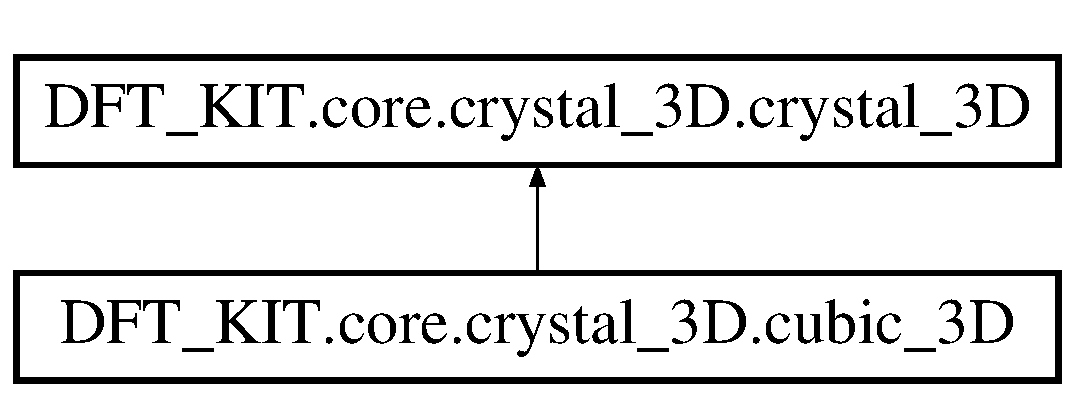
\includegraphics[height=2.000000cm]{class_d_f_t___k_i_t_1_1core_1_1crystal__3_d_1_1cubic__3_d}
\end{center}
\end{figure}
\subsection*{Public Member Functions}
\begin{DoxyCompactItemize}
\item 
def \hyperlink{class_d_f_t___k_i_t_1_1core_1_1crystal__3_d_1_1cubic__3_d_afb64ae6d89fa19d00038646c7c02956d}{\+\_\+\+\_\+init\+\_\+\+\_\+}
\item 
def \hyperlink{class_d_f_t___k_i_t_1_1core_1_1crystal__3_d_1_1cubic__3_d_ac17732ec3417c8748fc32439f101987a}{set\+\_\+lattice}
\item 
def \hyperlink{class_d_f_t___k_i_t_1_1core_1_1crystal__3_d_1_1cubic__3_d_a6f120c6e684c7dcdbf8f9e55df605e1b}{define\+\_\+klabels}
\end{DoxyCompactItemize}
\subsection*{Additional Inherited Members}


\subsection{Detailed Description}


Definition at line 143 of file crystal\+\_\+3\+D.\+py.



\subsection{Constructor \& Destructor Documentation}
\hypertarget{class_d_f_t___k_i_t_1_1core_1_1crystal__3_d_1_1cubic__3_d_afb64ae6d89fa19d00038646c7c02956d}{\index{D\+F\+T\+\_\+\+K\+I\+T\+::core\+::crystal\+\_\+3\+D\+::cubic\+\_\+3\+D@{D\+F\+T\+\_\+\+K\+I\+T\+::core\+::crystal\+\_\+3\+D\+::cubic\+\_\+3\+D}!\+\_\+\+\_\+init\+\_\+\+\_\+@{\+\_\+\+\_\+init\+\_\+\+\_\+}}
\index{\+\_\+\+\_\+init\+\_\+\+\_\+@{\+\_\+\+\_\+init\+\_\+\+\_\+}!D\+F\+T\+\_\+\+K\+I\+T\+::core\+::crystal\+\_\+3\+D\+::cubic\+\_\+3\+D@{D\+F\+T\+\_\+\+K\+I\+T\+::core\+::crystal\+\_\+3\+D\+::cubic\+\_\+3\+D}}
\subsubsection[{\+\_\+\+\_\+init\+\_\+\+\_\+}]{\setlength{\rightskip}{0pt plus 5cm}def D\+F\+T\+\_\+\+K\+I\+T.\+core.\+crystal\+\_\+3\+D.\+cubic\+\_\+3\+D.\+\_\+\+\_\+init\+\_\+\+\_\+ (
\begin{DoxyParamCaption}
\item[{}]{self, }
\item[{}]{cubic\+\_\+length, }
\item[{}]{length\+\_\+unit = {\ttfamily 1.0}}
\end{DoxyParamCaption}
)}}\label{class_d_f_t___k_i_t_1_1core_1_1crystal__3_d_1_1cubic__3_d_afb64ae6d89fa19d00038646c7c02956d}


Definition at line 144 of file crystal\+\_\+3\+D.\+py.



\subsection{Member Function Documentation}
\hypertarget{class_d_f_t___k_i_t_1_1core_1_1crystal__3_d_1_1cubic__3_d_a6f120c6e684c7dcdbf8f9e55df605e1b}{\index{D\+F\+T\+\_\+\+K\+I\+T\+::core\+::crystal\+\_\+3\+D\+::cubic\+\_\+3\+D@{D\+F\+T\+\_\+\+K\+I\+T\+::core\+::crystal\+\_\+3\+D\+::cubic\+\_\+3\+D}!define\+\_\+klabels@{define\+\_\+klabels}}
\index{define\+\_\+klabels@{define\+\_\+klabels}!D\+F\+T\+\_\+\+K\+I\+T\+::core\+::crystal\+\_\+3\+D\+::cubic\+\_\+3\+D@{D\+F\+T\+\_\+\+K\+I\+T\+::core\+::crystal\+\_\+3\+D\+::cubic\+\_\+3\+D}}
\subsubsection[{define\+\_\+klabels}]{\setlength{\rightskip}{0pt plus 5cm}def D\+F\+T\+\_\+\+K\+I\+T.\+core.\+crystal\+\_\+3\+D.\+cubic\+\_\+3\+D.\+define\+\_\+klabels (
\begin{DoxyParamCaption}
\item[{}]{self}
\end{DoxyParamCaption}
)}}\label{class_d_f_t___k_i_t_1_1core_1_1crystal__3_d_1_1cubic__3_d_a6f120c6e684c7dcdbf8f9e55df605e1b}


Definition at line 155 of file crystal\+\_\+3\+D.\+py.

\hypertarget{class_d_f_t___k_i_t_1_1core_1_1crystal__3_d_1_1cubic__3_d_ac17732ec3417c8748fc32439f101987a}{\index{D\+F\+T\+\_\+\+K\+I\+T\+::core\+::crystal\+\_\+3\+D\+::cubic\+\_\+3\+D@{D\+F\+T\+\_\+\+K\+I\+T\+::core\+::crystal\+\_\+3\+D\+::cubic\+\_\+3\+D}!set\+\_\+lattice@{set\+\_\+lattice}}
\index{set\+\_\+lattice@{set\+\_\+lattice}!D\+F\+T\+\_\+\+K\+I\+T\+::core\+::crystal\+\_\+3\+D\+::cubic\+\_\+3\+D@{D\+F\+T\+\_\+\+K\+I\+T\+::core\+::crystal\+\_\+3\+D\+::cubic\+\_\+3\+D}}
\subsubsection[{set\+\_\+lattice}]{\setlength{\rightskip}{0pt plus 5cm}def D\+F\+T\+\_\+\+K\+I\+T.\+core.\+crystal\+\_\+3\+D.\+cubic\+\_\+3\+D.\+set\+\_\+lattice (
\begin{DoxyParamCaption}
\item[{}]{self, }
\item[{}]{cubic\+\_\+length}
\end{DoxyParamCaption}
)}}\label{class_d_f_t___k_i_t_1_1core_1_1crystal__3_d_1_1cubic__3_d_ac17732ec3417c8748fc32439f101987a}


Definition at line 149 of file crystal\+\_\+3\+D.\+py.



The documentation for this class was generated from the following file\+:\begin{DoxyCompactItemize}
\item 
core/\hyperlink{crystal__3_d_8py}{crystal\+\_\+3\+D.\+py}\end{DoxyCompactItemize}

\hypertarget{class_d_f_t___k_i_t_1_1apps_1_1crystal__structure_1_1diamond}{\section{D\+F\+T\+\_\+\+K\+I\+T.\+apps.\+crystal\+\_\+structure.\+diamond Class Reference}
\label{class_d_f_t___k_i_t_1_1apps_1_1crystal__structure_1_1diamond}\index{D\+F\+T\+\_\+\+K\+I\+T.\+apps.\+crystal\+\_\+structure.\+diamond@{D\+F\+T\+\_\+\+K\+I\+T.\+apps.\+crystal\+\_\+structure.\+diamond}}
}
Inheritance diagram for D\+F\+T\+\_\+\+K\+I\+T.\+apps.\+crystal\+\_\+structure.\+diamond\+:\begin{figure}[H]
\begin{center}
\leavevmode
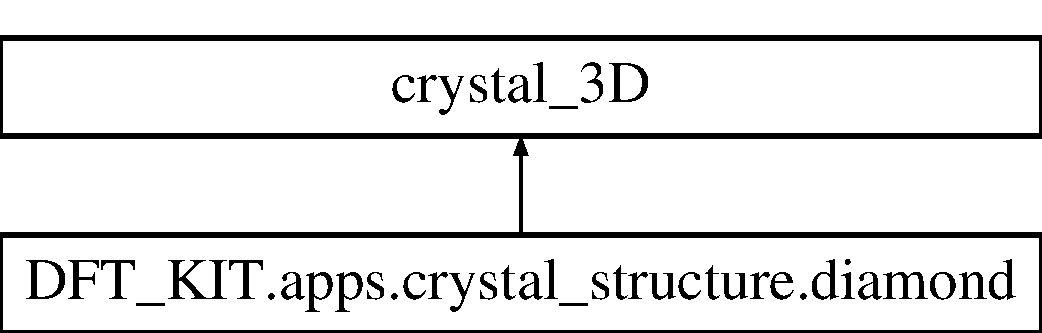
\includegraphics[height=2.000000cm]{class_d_f_t___k_i_t_1_1apps_1_1crystal__structure_1_1diamond}
\end{center}
\end{figure}
\subsection*{Public Member Functions}
\begin{DoxyCompactItemize}
\item 
def \hyperlink{class_d_f_t___k_i_t_1_1apps_1_1crystal__structure_1_1diamond_a26b84c35323c47bc7162c3821b7fd2fa}{\+\_\+\+\_\+init\+\_\+\+\_\+}
\end{DoxyCompactItemize}


\subsection{Detailed Description}


Definition at line 48 of file crystal\+\_\+structure.\+py.



\subsection{Constructor \& Destructor Documentation}
\hypertarget{class_d_f_t___k_i_t_1_1apps_1_1crystal__structure_1_1diamond_a26b84c35323c47bc7162c3821b7fd2fa}{\index{D\+F\+T\+\_\+\+K\+I\+T\+::apps\+::crystal\+\_\+structure\+::diamond@{D\+F\+T\+\_\+\+K\+I\+T\+::apps\+::crystal\+\_\+structure\+::diamond}!\+\_\+\+\_\+init\+\_\+\+\_\+@{\+\_\+\+\_\+init\+\_\+\+\_\+}}
\index{\+\_\+\+\_\+init\+\_\+\+\_\+@{\+\_\+\+\_\+init\+\_\+\+\_\+}!D\+F\+T\+\_\+\+K\+I\+T\+::apps\+::crystal\+\_\+structure\+::diamond@{D\+F\+T\+\_\+\+K\+I\+T\+::apps\+::crystal\+\_\+structure\+::diamond}}
\subsubsection[{\+\_\+\+\_\+init\+\_\+\+\_\+}]{\setlength{\rightskip}{0pt plus 5cm}def D\+F\+T\+\_\+\+K\+I\+T.\+apps.\+crystal\+\_\+structure.\+diamond.\+\_\+\+\_\+init\+\_\+\+\_\+ (
\begin{DoxyParamCaption}
\item[{}]{self, }
\item[{}]{length\+\_\+unit = {\ttfamily 1.0}}
\end{DoxyParamCaption}
)}}\label{class_d_f_t___k_i_t_1_1apps_1_1crystal__structure_1_1diamond_a26b84c35323c47bc7162c3821b7fd2fa}


Definition at line 49 of file crystal\+\_\+structure.\+py.



The documentation for this class was generated from the following file\+:\begin{DoxyCompactItemize}
\item 
apps/\hyperlink{crystal__structure_8py}{crystal\+\_\+structure.\+py}\end{DoxyCompactItemize}

\hypertarget{class_d_f_t___k_i_t_1_1core_1_1element_1_1element}{\section{D\+F\+T\+\_\+\+K\+I\+T.\+core.\+element.\+element Class Reference}
\label{class_d_f_t___k_i_t_1_1core_1_1element_1_1element}\index{D\+F\+T\+\_\+\+K\+I\+T.\+core.\+element.\+element@{D\+F\+T\+\_\+\+K\+I\+T.\+core.\+element.\+element}}
}
\subsection*{Public Member Functions}
\begin{DoxyCompactItemize}
\item 
def \hyperlink{class_d_f_t___k_i_t_1_1core_1_1element_1_1element_a6b8ca9cda88a43aff0d4fae80d3e06f3}{\+\_\+\+\_\+init\+\_\+\+\_\+}
\end{DoxyCompactItemize}
\subsection*{Public Attributes}
\begin{DoxyCompactItemize}
\item 
\hyperlink{class_d_f_t___k_i_t_1_1core_1_1element_1_1element_ab2919368378ec5a3c88f561701437ca0}{symbol}
\item 
\hyperlink{class_d_f_t___k_i_t_1_1core_1_1element_1_1element_a798861de085eb85aebbcdedd54371731}{mass}
\item 
\hyperlink{class_d_f_t___k_i_t_1_1core_1_1element_1_1element_a9fdfc898296fd99c70addb3a7f9d7616}{nuc\+Z}
\item 
\hyperlink{class_d_f_t___k_i_t_1_1core_1_1element_1_1element_af0b4a1138ddc637879efb7f1dfc96630}{vale}
\item 
\hyperlink{class_d_f_t___k_i_t_1_1core_1_1element_1_1element_a351a8d8ba25af9024aee42cec88fc993}{info}
\end{DoxyCompactItemize}


\subsection{Detailed Description}


Definition at line 45 of file element.\+py.



\subsection{Constructor \& Destructor Documentation}
\hypertarget{class_d_f_t___k_i_t_1_1core_1_1element_1_1element_a6b8ca9cda88a43aff0d4fae80d3e06f3}{\index{D\+F\+T\+\_\+\+K\+I\+T\+::core\+::element\+::element@{D\+F\+T\+\_\+\+K\+I\+T\+::core\+::element\+::element}!\+\_\+\+\_\+init\+\_\+\+\_\+@{\+\_\+\+\_\+init\+\_\+\+\_\+}}
\index{\+\_\+\+\_\+init\+\_\+\+\_\+@{\+\_\+\+\_\+init\+\_\+\+\_\+}!D\+F\+T\+\_\+\+K\+I\+T\+::core\+::element\+::element@{D\+F\+T\+\_\+\+K\+I\+T\+::core\+::element\+::element}}
\subsubsection[{\+\_\+\+\_\+init\+\_\+\+\_\+}]{\setlength{\rightskip}{0pt plus 5cm}def D\+F\+T\+\_\+\+K\+I\+T.\+core.\+element.\+element.\+\_\+\+\_\+init\+\_\+\+\_\+ (
\begin{DoxyParamCaption}
\item[{}]{self, }
\item[{}]{symbol = {\ttfamily None}, }
\item[{}]{mass = {\ttfamily None}, }
\item[{}]{nuc\+Z = {\ttfamily None}, }
\item[{}]{vale = {\ttfamily None}, }
\item[{}]{info}
\end{DoxyParamCaption}
)}}\label{class_d_f_t___k_i_t_1_1core_1_1element_1_1element_a6b8ca9cda88a43aff0d4fae80d3e06f3}


Definition at line 46 of file element.\+py.



\subsection{Member Data Documentation}
\hypertarget{class_d_f_t___k_i_t_1_1core_1_1element_1_1element_a351a8d8ba25af9024aee42cec88fc993}{\index{D\+F\+T\+\_\+\+K\+I\+T\+::core\+::element\+::element@{D\+F\+T\+\_\+\+K\+I\+T\+::core\+::element\+::element}!info@{info}}
\index{info@{info}!D\+F\+T\+\_\+\+K\+I\+T\+::core\+::element\+::element@{D\+F\+T\+\_\+\+K\+I\+T\+::core\+::element\+::element}}
\subsubsection[{info}]{\setlength{\rightskip}{0pt plus 5cm}D\+F\+T\+\_\+\+K\+I\+T.\+core.\+element.\+element.\+info}}\label{class_d_f_t___k_i_t_1_1core_1_1element_1_1element_a351a8d8ba25af9024aee42cec88fc993}


Definition at line 51 of file element.\+py.

\hypertarget{class_d_f_t___k_i_t_1_1core_1_1element_1_1element_a798861de085eb85aebbcdedd54371731}{\index{D\+F\+T\+\_\+\+K\+I\+T\+::core\+::element\+::element@{D\+F\+T\+\_\+\+K\+I\+T\+::core\+::element\+::element}!mass@{mass}}
\index{mass@{mass}!D\+F\+T\+\_\+\+K\+I\+T\+::core\+::element\+::element@{D\+F\+T\+\_\+\+K\+I\+T\+::core\+::element\+::element}}
\subsubsection[{mass}]{\setlength{\rightskip}{0pt plus 5cm}D\+F\+T\+\_\+\+K\+I\+T.\+core.\+element.\+element.\+mass}}\label{class_d_f_t___k_i_t_1_1core_1_1element_1_1element_a798861de085eb85aebbcdedd54371731}


Definition at line 48 of file element.\+py.

\hypertarget{class_d_f_t___k_i_t_1_1core_1_1element_1_1element_a9fdfc898296fd99c70addb3a7f9d7616}{\index{D\+F\+T\+\_\+\+K\+I\+T\+::core\+::element\+::element@{D\+F\+T\+\_\+\+K\+I\+T\+::core\+::element\+::element}!nuc\+Z@{nuc\+Z}}
\index{nuc\+Z@{nuc\+Z}!D\+F\+T\+\_\+\+K\+I\+T\+::core\+::element\+::element@{D\+F\+T\+\_\+\+K\+I\+T\+::core\+::element\+::element}}
\subsubsection[{nuc\+Z}]{\setlength{\rightskip}{0pt plus 5cm}D\+F\+T\+\_\+\+K\+I\+T.\+core.\+element.\+element.\+nuc\+Z}}\label{class_d_f_t___k_i_t_1_1core_1_1element_1_1element_a9fdfc898296fd99c70addb3a7f9d7616}


Definition at line 49 of file element.\+py.

\hypertarget{class_d_f_t___k_i_t_1_1core_1_1element_1_1element_ab2919368378ec5a3c88f561701437ca0}{\index{D\+F\+T\+\_\+\+K\+I\+T\+::core\+::element\+::element@{D\+F\+T\+\_\+\+K\+I\+T\+::core\+::element\+::element}!symbol@{symbol}}
\index{symbol@{symbol}!D\+F\+T\+\_\+\+K\+I\+T\+::core\+::element\+::element@{D\+F\+T\+\_\+\+K\+I\+T\+::core\+::element\+::element}}
\subsubsection[{symbol}]{\setlength{\rightskip}{0pt plus 5cm}D\+F\+T\+\_\+\+K\+I\+T.\+core.\+element.\+element.\+symbol}}\label{class_d_f_t___k_i_t_1_1core_1_1element_1_1element_ab2919368378ec5a3c88f561701437ca0}


Definition at line 47 of file element.\+py.

\hypertarget{class_d_f_t___k_i_t_1_1core_1_1element_1_1element_af0b4a1138ddc637879efb7f1dfc96630}{\index{D\+F\+T\+\_\+\+K\+I\+T\+::core\+::element\+::element@{D\+F\+T\+\_\+\+K\+I\+T\+::core\+::element\+::element}!vale@{vale}}
\index{vale@{vale}!D\+F\+T\+\_\+\+K\+I\+T\+::core\+::element\+::element@{D\+F\+T\+\_\+\+K\+I\+T\+::core\+::element\+::element}}
\subsubsection[{vale}]{\setlength{\rightskip}{0pt plus 5cm}D\+F\+T\+\_\+\+K\+I\+T.\+core.\+element.\+element.\+vale}}\label{class_d_f_t___k_i_t_1_1core_1_1element_1_1element_af0b4a1138ddc637879efb7f1dfc96630}


Definition at line 50 of file element.\+py.



The documentation for this class was generated from the following file\+:\begin{DoxyCompactItemize}
\item 
core/\hyperlink{element_8py}{element.\+py}\end{DoxyCompactItemize}

\hypertarget{class_d_f_t___k_i_t_1_1apps_1_1crystal__structure_1_1face__center}{\section{D\+F\+T\+\_\+\+K\+I\+T.\+apps.\+crystal\+\_\+structure.\+face\+\_\+center Class Reference}
\label{class_d_f_t___k_i_t_1_1apps_1_1crystal__structure_1_1face__center}\index{D\+F\+T\+\_\+\+K\+I\+T.\+apps.\+crystal\+\_\+structure.\+face\+\_\+center@{D\+F\+T\+\_\+\+K\+I\+T.\+apps.\+crystal\+\_\+structure.\+face\+\_\+center}}
}
Inheritance diagram for D\+F\+T\+\_\+\+K\+I\+T.\+apps.\+crystal\+\_\+structure.\+face\+\_\+center\+:\begin{figure}[H]
\begin{center}
\leavevmode
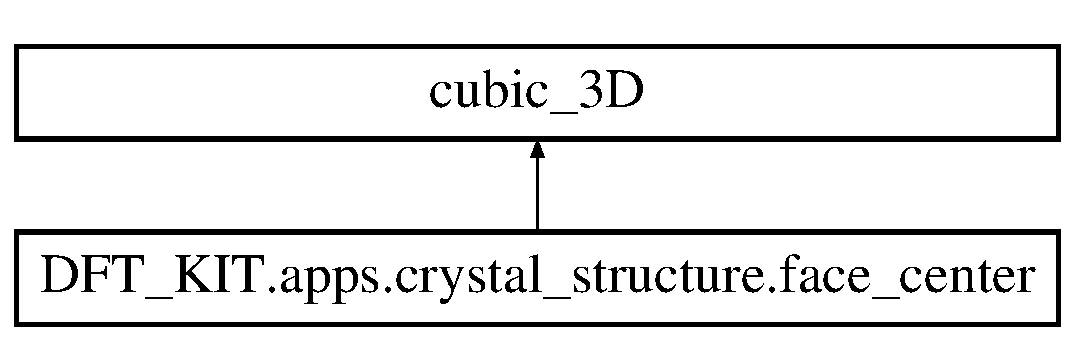
\includegraphics[height=2.000000cm]{class_d_f_t___k_i_t_1_1apps_1_1crystal__structure_1_1face__center}
\end{center}
\end{figure}
\subsection*{Public Member Functions}
\begin{DoxyCompactItemize}
\item 
def \hyperlink{class_d_f_t___k_i_t_1_1apps_1_1crystal__structure_1_1face__center_a8c00236923b634233a4c8d7c479ca620}{\+\_\+\+\_\+init\+\_\+\+\_\+}
\end{DoxyCompactItemize}


\subsection{Detailed Description}


Definition at line 64 of file crystal\+\_\+structure.\+py.



\subsection{Constructor \& Destructor Documentation}
\hypertarget{class_d_f_t___k_i_t_1_1apps_1_1crystal__structure_1_1face__center_a8c00236923b634233a4c8d7c479ca620}{\index{D\+F\+T\+\_\+\+K\+I\+T\+::apps\+::crystal\+\_\+structure\+::face\+\_\+center@{D\+F\+T\+\_\+\+K\+I\+T\+::apps\+::crystal\+\_\+structure\+::face\+\_\+center}!\+\_\+\+\_\+init\+\_\+\+\_\+@{\+\_\+\+\_\+init\+\_\+\+\_\+}}
\index{\+\_\+\+\_\+init\+\_\+\+\_\+@{\+\_\+\+\_\+init\+\_\+\+\_\+}!D\+F\+T\+\_\+\+K\+I\+T\+::apps\+::crystal\+\_\+structure\+::face\+\_\+center@{D\+F\+T\+\_\+\+K\+I\+T\+::apps\+::crystal\+\_\+structure\+::face\+\_\+center}}
\subsubsection[{\+\_\+\+\_\+init\+\_\+\+\_\+}]{\setlength{\rightskip}{0pt plus 5cm}def D\+F\+T\+\_\+\+K\+I\+T.\+apps.\+crystal\+\_\+structure.\+face\+\_\+center.\+\_\+\+\_\+init\+\_\+\+\_\+ (
\begin{DoxyParamCaption}
\item[{}]{self, }
\item[{}]{cubic\+\_\+length, }
\item[{}]{length\+\_\+unit = {\ttfamily 1.0}}
\end{DoxyParamCaption}
)}}\label{class_d_f_t___k_i_t_1_1apps_1_1crystal__structure_1_1face__center_a8c00236923b634233a4c8d7c479ca620}


Definition at line 65 of file crystal\+\_\+structure.\+py.



The documentation for this class was generated from the following file\+:\begin{DoxyCompactItemize}
\item 
apps/\hyperlink{crystal__structure_8py}{crystal\+\_\+structure.\+py}\end{DoxyCompactItemize}

\hypertarget{class_d_f_t___k_i_t_1_1core_1_1crystal__3_d_1_1fcc__3_d}{\section{D\+F\+T\+\_\+\+K\+I\+T.\+core.\+crystal\+\_\+3\+D.\+fcc\+\_\+3\+D Class Reference}
\label{class_d_f_t___k_i_t_1_1core_1_1crystal__3_d_1_1fcc__3_d}\index{D\+F\+T\+\_\+\+K\+I\+T.\+core.\+crystal\+\_\+3\+D.\+fcc\+\_\+3\+D@{D\+F\+T\+\_\+\+K\+I\+T.\+core.\+crystal\+\_\+3\+D.\+fcc\+\_\+3\+D}}
}
Inheritance diagram for D\+F\+T\+\_\+\+K\+I\+T.\+core.\+crystal\+\_\+3\+D.\+fcc\+\_\+3\+D\+:\begin{figure}[H]
\begin{center}
\leavevmode
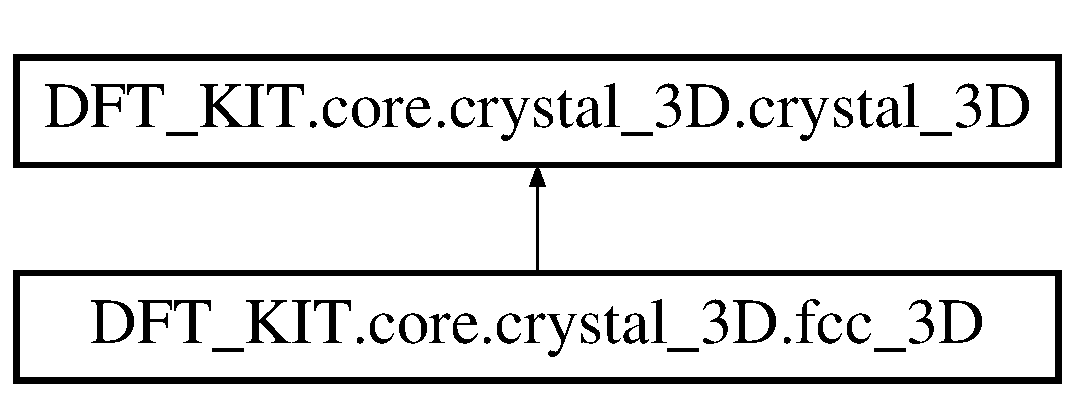
\includegraphics[height=2.000000cm]{class_d_f_t___k_i_t_1_1core_1_1crystal__3_d_1_1fcc__3_d}
\end{center}
\end{figure}
\subsection*{Public Member Functions}
\begin{DoxyCompactItemize}
\item 
def \hyperlink{class_d_f_t___k_i_t_1_1core_1_1crystal__3_d_1_1fcc__3_d_abdd976094ae54ffb6cf6302a2fe0928a}{\+\_\+\+\_\+init\+\_\+\+\_\+}
\item 
def \hyperlink{class_d_f_t___k_i_t_1_1core_1_1crystal__3_d_1_1fcc__3_d_ab33239aebb5e2714120fbb3691e1a200}{set\+\_\+lattice}
\item 
def \hyperlink{class_d_f_t___k_i_t_1_1core_1_1crystal__3_d_1_1fcc__3_d_a50cd517a076d6d633c81841aa53b9595}{define\+\_\+klabels}
\end{DoxyCompactItemize}
\subsection*{Additional Inherited Members}


\subsection{Detailed Description}


Definition at line 195 of file crystal\+\_\+3\+D.\+py.



\subsection{Constructor \& Destructor Documentation}
\hypertarget{class_d_f_t___k_i_t_1_1core_1_1crystal__3_d_1_1fcc__3_d_abdd976094ae54ffb6cf6302a2fe0928a}{\index{D\+F\+T\+\_\+\+K\+I\+T\+::core\+::crystal\+\_\+3\+D\+::fcc\+\_\+3\+D@{D\+F\+T\+\_\+\+K\+I\+T\+::core\+::crystal\+\_\+3\+D\+::fcc\+\_\+3\+D}!\+\_\+\+\_\+init\+\_\+\+\_\+@{\+\_\+\+\_\+init\+\_\+\+\_\+}}
\index{\+\_\+\+\_\+init\+\_\+\+\_\+@{\+\_\+\+\_\+init\+\_\+\+\_\+}!D\+F\+T\+\_\+\+K\+I\+T\+::core\+::crystal\+\_\+3\+D\+::fcc\+\_\+3\+D@{D\+F\+T\+\_\+\+K\+I\+T\+::core\+::crystal\+\_\+3\+D\+::fcc\+\_\+3\+D}}
\subsubsection[{\+\_\+\+\_\+init\+\_\+\+\_\+}]{\setlength{\rightskip}{0pt plus 5cm}def D\+F\+T\+\_\+\+K\+I\+T.\+core.\+crystal\+\_\+3\+D.\+fcc\+\_\+3\+D.\+\_\+\+\_\+init\+\_\+\+\_\+ (
\begin{DoxyParamCaption}
\item[{}]{self, }
\item[{}]{fcc\+\_\+length, }
\item[{}]{length\+\_\+unit = {\ttfamily 1.0}}
\end{DoxyParamCaption}
)}}\label{class_d_f_t___k_i_t_1_1core_1_1crystal__3_d_1_1fcc__3_d_abdd976094ae54ffb6cf6302a2fe0928a}


Definition at line 196 of file crystal\+\_\+3\+D.\+py.



\subsection{Member Function Documentation}
\hypertarget{class_d_f_t___k_i_t_1_1core_1_1crystal__3_d_1_1fcc__3_d_a50cd517a076d6d633c81841aa53b9595}{\index{D\+F\+T\+\_\+\+K\+I\+T\+::core\+::crystal\+\_\+3\+D\+::fcc\+\_\+3\+D@{D\+F\+T\+\_\+\+K\+I\+T\+::core\+::crystal\+\_\+3\+D\+::fcc\+\_\+3\+D}!define\+\_\+klabels@{define\+\_\+klabels}}
\index{define\+\_\+klabels@{define\+\_\+klabels}!D\+F\+T\+\_\+\+K\+I\+T\+::core\+::crystal\+\_\+3\+D\+::fcc\+\_\+3\+D@{D\+F\+T\+\_\+\+K\+I\+T\+::core\+::crystal\+\_\+3\+D\+::fcc\+\_\+3\+D}}
\subsubsection[{define\+\_\+klabels}]{\setlength{\rightskip}{0pt plus 5cm}def D\+F\+T\+\_\+\+K\+I\+T.\+core.\+crystal\+\_\+3\+D.\+fcc\+\_\+3\+D.\+define\+\_\+klabels (
\begin{DoxyParamCaption}
\item[{}]{self}
\end{DoxyParamCaption}
)}}\label{class_d_f_t___k_i_t_1_1core_1_1crystal__3_d_1_1fcc__3_d_a50cd517a076d6d633c81841aa53b9595}


Definition at line 208 of file crystal\+\_\+3\+D.\+py.

\hypertarget{class_d_f_t___k_i_t_1_1core_1_1crystal__3_d_1_1fcc__3_d_ab33239aebb5e2714120fbb3691e1a200}{\index{D\+F\+T\+\_\+\+K\+I\+T\+::core\+::crystal\+\_\+3\+D\+::fcc\+\_\+3\+D@{D\+F\+T\+\_\+\+K\+I\+T\+::core\+::crystal\+\_\+3\+D\+::fcc\+\_\+3\+D}!set\+\_\+lattice@{set\+\_\+lattice}}
\index{set\+\_\+lattice@{set\+\_\+lattice}!D\+F\+T\+\_\+\+K\+I\+T\+::core\+::crystal\+\_\+3\+D\+::fcc\+\_\+3\+D@{D\+F\+T\+\_\+\+K\+I\+T\+::core\+::crystal\+\_\+3\+D\+::fcc\+\_\+3\+D}}
\subsubsection[{set\+\_\+lattice}]{\setlength{\rightskip}{0pt plus 5cm}def D\+F\+T\+\_\+\+K\+I\+T.\+core.\+crystal\+\_\+3\+D.\+fcc\+\_\+3\+D.\+set\+\_\+lattice (
\begin{DoxyParamCaption}
\item[{}]{self, }
\item[{}]{fcc\+\_\+length}
\end{DoxyParamCaption}
)}}\label{class_d_f_t___k_i_t_1_1core_1_1crystal__3_d_1_1fcc__3_d_ab33239aebb5e2714120fbb3691e1a200}


Definition at line 201 of file crystal\+\_\+3\+D.\+py.



The documentation for this class was generated from the following file\+:\begin{DoxyCompactItemize}
\item 
core/\hyperlink{crystal__3_d_8py}{crystal\+\_\+3\+D.\+py}\end{DoxyCompactItemize}

\hypertarget{class_d_f_t___k_i_t_1_1apps_1_1crystal__structure_1_1graphene}{\section{D\+F\+T\+\_\+\+K\+I\+T.\+apps.\+crystal\+\_\+structure.\+graphene Class Reference}
\label{class_d_f_t___k_i_t_1_1apps_1_1crystal__structure_1_1graphene}\index{D\+F\+T\+\_\+\+K\+I\+T.\+apps.\+crystal\+\_\+structure.\+graphene@{D\+F\+T\+\_\+\+K\+I\+T.\+apps.\+crystal\+\_\+structure.\+graphene}}
}
Inheritance diagram for D\+F\+T\+\_\+\+K\+I\+T.\+apps.\+crystal\+\_\+structure.\+graphene\+:\begin{figure}[H]
\begin{center}
\leavevmode
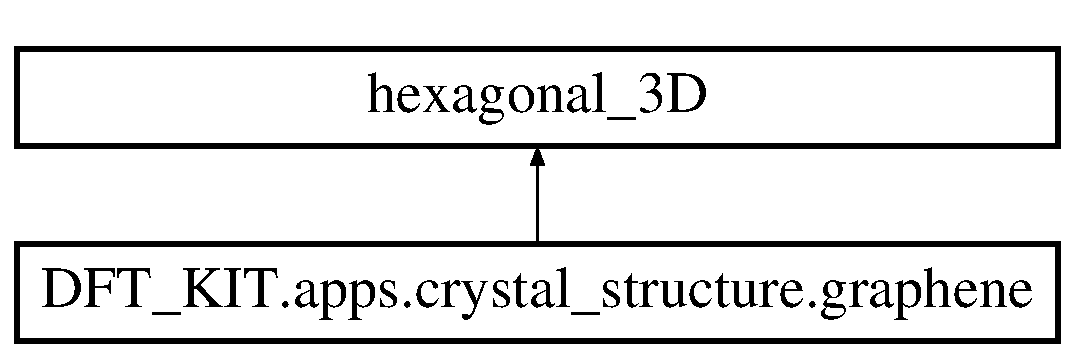
\includegraphics[height=2.000000cm]{class_d_f_t___k_i_t_1_1apps_1_1crystal__structure_1_1graphene}
\end{center}
\end{figure}
\subsection*{Public Member Functions}
\begin{DoxyCompactItemize}
\item 
def \hyperlink{class_d_f_t___k_i_t_1_1apps_1_1crystal__structure_1_1graphene_a70c251011fedfe4b3350b18405a67c5b}{\+\_\+\+\_\+init\+\_\+\+\_\+}
\end{DoxyCompactItemize}


\subsection{Detailed Description}


Definition at line 35 of file crystal\+\_\+structure.\+py.



\subsection{Constructor \& Destructor Documentation}
\hypertarget{class_d_f_t___k_i_t_1_1apps_1_1crystal__structure_1_1graphene_a70c251011fedfe4b3350b18405a67c5b}{\index{D\+F\+T\+\_\+\+K\+I\+T\+::apps\+::crystal\+\_\+structure\+::graphene@{D\+F\+T\+\_\+\+K\+I\+T\+::apps\+::crystal\+\_\+structure\+::graphene}!\+\_\+\+\_\+init\+\_\+\+\_\+@{\+\_\+\+\_\+init\+\_\+\+\_\+}}
\index{\+\_\+\+\_\+init\+\_\+\+\_\+@{\+\_\+\+\_\+init\+\_\+\+\_\+}!D\+F\+T\+\_\+\+K\+I\+T\+::apps\+::crystal\+\_\+structure\+::graphene@{D\+F\+T\+\_\+\+K\+I\+T\+::apps\+::crystal\+\_\+structure\+::graphene}}
\subsubsection[{\+\_\+\+\_\+init\+\_\+\+\_\+}]{\setlength{\rightskip}{0pt plus 5cm}def D\+F\+T\+\_\+\+K\+I\+T.\+apps.\+crystal\+\_\+structure.\+graphene.\+\_\+\+\_\+init\+\_\+\+\_\+ (
\begin{DoxyParamCaption}
\item[{}]{self, }
\item[{}]{element, }
\item[{}]{hex\+\_\+a\+\_\+length, }
\item[{}]{hex\+\_\+c\+\_\+length, }
\item[{}]{length\+\_\+unit = {\ttfamily 1.0}, }
\item[{}]{parms}
\end{DoxyParamCaption}
)}}\label{class_d_f_t___k_i_t_1_1apps_1_1crystal__structure_1_1graphene_a70c251011fedfe4b3350b18405a67c5b}


Definition at line 36 of file crystal\+\_\+structure.\+py.



The documentation for this class was generated from the following file\+:\begin{DoxyCompactItemize}
\item 
apps/\hyperlink{crystal__structure_8py}{crystal\+\_\+structure.\+py}\end{DoxyCompactItemize}

\hypertarget{class_d_f_t___k_i_t_1_1core_1_1crystal__3_d_1_1hexagonal__3_d}{\section{D\+F\+T\+\_\+\+K\+I\+T.\+core.\+crystal\+\_\+3\+D.\+hexagonal\+\_\+3\+D Class Reference}
\label{class_d_f_t___k_i_t_1_1core_1_1crystal__3_d_1_1hexagonal__3_d}\index{D\+F\+T\+\_\+\+K\+I\+T.\+core.\+crystal\+\_\+3\+D.\+hexagonal\+\_\+3\+D@{D\+F\+T\+\_\+\+K\+I\+T.\+core.\+crystal\+\_\+3\+D.\+hexagonal\+\_\+3\+D}}
}
Inheritance diagram for D\+F\+T\+\_\+\+K\+I\+T.\+core.\+crystal\+\_\+3\+D.\+hexagonal\+\_\+3\+D\+:\begin{figure}[H]
\begin{center}
\leavevmode
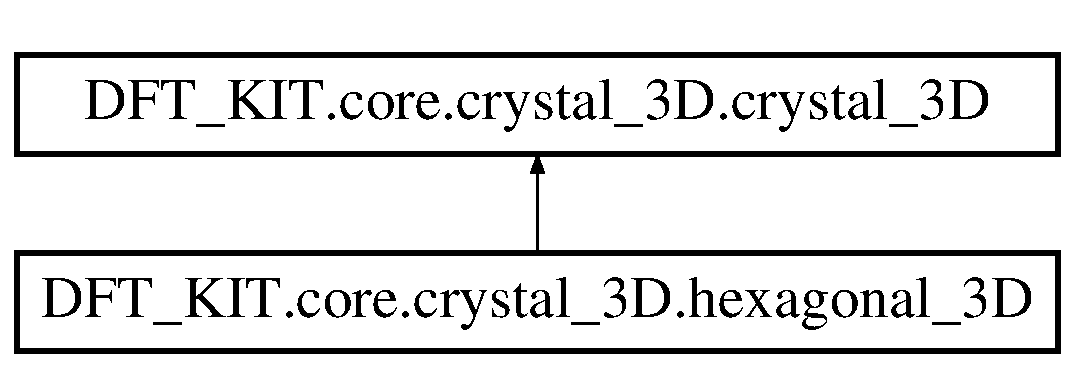
\includegraphics[height=2.000000cm]{class_d_f_t___k_i_t_1_1core_1_1crystal__3_d_1_1hexagonal__3_d}
\end{center}
\end{figure}
\subsection*{Public Member Functions}
\begin{DoxyCompactItemize}
\item 
def \hyperlink{class_d_f_t___k_i_t_1_1core_1_1crystal__3_d_1_1hexagonal__3_d_acf922212dc726c10f1377733bdfbbf60}{\+\_\+\+\_\+init\+\_\+\+\_\+}
\item 
def \hyperlink{class_d_f_t___k_i_t_1_1core_1_1crystal__3_d_1_1hexagonal__3_d_a8d3268633d8f2ae7014c1051c60639fe}{set\+\_\+lattice}
\item 
def \hyperlink{class_d_f_t___k_i_t_1_1core_1_1crystal__3_d_1_1hexagonal__3_d_aedd3173cbf84663166eeae0c78f4f3bc}{define\+\_\+klabels}
\end{DoxyCompactItemize}
\subsection*{Additional Inherited Members}


\subsection{Detailed Description}


Definition at line 222 of file crystal\+\_\+3\+D.\+py.



\subsection{Constructor \& Destructor Documentation}
\hypertarget{class_d_f_t___k_i_t_1_1core_1_1crystal__3_d_1_1hexagonal__3_d_acf922212dc726c10f1377733bdfbbf60}{\index{D\+F\+T\+\_\+\+K\+I\+T\+::core\+::crystal\+\_\+3\+D\+::hexagonal\+\_\+3\+D@{D\+F\+T\+\_\+\+K\+I\+T\+::core\+::crystal\+\_\+3\+D\+::hexagonal\+\_\+3\+D}!\+\_\+\+\_\+init\+\_\+\+\_\+@{\+\_\+\+\_\+init\+\_\+\+\_\+}}
\index{\+\_\+\+\_\+init\+\_\+\+\_\+@{\+\_\+\+\_\+init\+\_\+\+\_\+}!D\+F\+T\+\_\+\+K\+I\+T\+::core\+::crystal\+\_\+3\+D\+::hexagonal\+\_\+3\+D@{D\+F\+T\+\_\+\+K\+I\+T\+::core\+::crystal\+\_\+3\+D\+::hexagonal\+\_\+3\+D}}
\subsubsection[{\+\_\+\+\_\+init\+\_\+\+\_\+}]{\setlength{\rightskip}{0pt plus 5cm}def D\+F\+T\+\_\+\+K\+I\+T.\+core.\+crystal\+\_\+3\+D.\+hexagonal\+\_\+3\+D.\+\_\+\+\_\+init\+\_\+\+\_\+ (
\begin{DoxyParamCaption}
\item[{}]{self, }
\item[{}]{hex\+\_\+a\+\_\+length, }
\item[{}]{hex\+\_\+c\+\_\+length, }
\item[{}]{length\+\_\+unit = {\ttfamily 1.0}}
\end{DoxyParamCaption}
)}}\label{class_d_f_t___k_i_t_1_1core_1_1crystal__3_d_1_1hexagonal__3_d_acf922212dc726c10f1377733bdfbbf60}


Definition at line 223 of file crystal\+\_\+3\+D.\+py.



\subsection{Member Function Documentation}
\hypertarget{class_d_f_t___k_i_t_1_1core_1_1crystal__3_d_1_1hexagonal__3_d_aedd3173cbf84663166eeae0c78f4f3bc}{\index{D\+F\+T\+\_\+\+K\+I\+T\+::core\+::crystal\+\_\+3\+D\+::hexagonal\+\_\+3\+D@{D\+F\+T\+\_\+\+K\+I\+T\+::core\+::crystal\+\_\+3\+D\+::hexagonal\+\_\+3\+D}!define\+\_\+klabels@{define\+\_\+klabels}}
\index{define\+\_\+klabels@{define\+\_\+klabels}!D\+F\+T\+\_\+\+K\+I\+T\+::core\+::crystal\+\_\+3\+D\+::hexagonal\+\_\+3\+D@{D\+F\+T\+\_\+\+K\+I\+T\+::core\+::crystal\+\_\+3\+D\+::hexagonal\+\_\+3\+D}}
\subsubsection[{define\+\_\+klabels}]{\setlength{\rightskip}{0pt plus 5cm}def D\+F\+T\+\_\+\+K\+I\+T.\+core.\+crystal\+\_\+3\+D.\+hexagonal\+\_\+3\+D.\+define\+\_\+klabels (
\begin{DoxyParamCaption}
\item[{}]{self}
\end{DoxyParamCaption}
)}}\label{class_d_f_t___k_i_t_1_1core_1_1crystal__3_d_1_1hexagonal__3_d_aedd3173cbf84663166eeae0c78f4f3bc}


Definition at line 235 of file crystal\+\_\+3\+D.\+py.

\hypertarget{class_d_f_t___k_i_t_1_1core_1_1crystal__3_d_1_1hexagonal__3_d_a8d3268633d8f2ae7014c1051c60639fe}{\index{D\+F\+T\+\_\+\+K\+I\+T\+::core\+::crystal\+\_\+3\+D\+::hexagonal\+\_\+3\+D@{D\+F\+T\+\_\+\+K\+I\+T\+::core\+::crystal\+\_\+3\+D\+::hexagonal\+\_\+3\+D}!set\+\_\+lattice@{set\+\_\+lattice}}
\index{set\+\_\+lattice@{set\+\_\+lattice}!D\+F\+T\+\_\+\+K\+I\+T\+::core\+::crystal\+\_\+3\+D\+::hexagonal\+\_\+3\+D@{D\+F\+T\+\_\+\+K\+I\+T\+::core\+::crystal\+\_\+3\+D\+::hexagonal\+\_\+3\+D}}
\subsubsection[{set\+\_\+lattice}]{\setlength{\rightskip}{0pt plus 5cm}def D\+F\+T\+\_\+\+K\+I\+T.\+core.\+crystal\+\_\+3\+D.\+hexagonal\+\_\+3\+D.\+set\+\_\+lattice (
\begin{DoxyParamCaption}
\item[{}]{self, }
\item[{}]{hex\+\_\+a\+\_\+length, }
\item[{}]{hex\+\_\+c\+\_\+length}
\end{DoxyParamCaption}
)}}\label{class_d_f_t___k_i_t_1_1core_1_1crystal__3_d_1_1hexagonal__3_d_a8d3268633d8f2ae7014c1051c60639fe}


Definition at line 228 of file crystal\+\_\+3\+D.\+py.



The documentation for this class was generated from the following file\+:\begin{DoxyCompactItemize}
\item 
core/\hyperlink{crystal__3_d_8py}{crystal\+\_\+3\+D.\+py}\end{DoxyCompactItemize}

\hypertarget{class_d_f_t___k_i_t_1_1core_1_1job_1_1job}{\section{D\+F\+T\+\_\+\+K\+I\+T.\+core.\+job.\+job Class Reference}
\label{class_d_f_t___k_i_t_1_1core_1_1job_1_1job}\index{D\+F\+T\+\_\+\+K\+I\+T.\+core.\+job.\+job@{D\+F\+T\+\_\+\+K\+I\+T.\+core.\+job.\+job}}
}
\subsection*{Public Member Functions}
\begin{DoxyCompactItemize}
\item 
def \hyperlink{class_d_f_t___k_i_t_1_1core_1_1job_1_1job_a98042c98ccedc93756b3c7e7696a701e}{\+\_\+\+\_\+init\+\_\+\+\_\+}
\item 
def \hyperlink{class_d_f_t___k_i_t_1_1core_1_1job_1_1job_a24e78596f2fd5f7ff326c548a5570e8e}{set\+\_\+sysinfo}
\item 
def \hyperlink{class_d_f_t___k_i_t_1_1core_1_1job_1_1job_aff31da650d3d93fee45f1422387cf720}{get\+\_\+sysinfo}
\item 
def \hyperlink{class_d_f_t___k_i_t_1_1core_1_1job_1_1job_a2eaf8ac59a5f04cfd0108ae3c9e061f1}{get\+\_\+maindir}
\item 
def \hyperlink{class_d_f_t___k_i_t_1_1core_1_1job_1_1job_a6e1d361a90d70216572c62a3d75c62b9}{set\+\_\+verbosity}
\item 
def \hyperlink{class_d_f_t___k_i_t_1_1core_1_1job_1_1job_ac4e8212ce995ff57582d1c2855416d13}{show\+\_\+verbose}
\item 
def \hyperlink{class_d_f_t___k_i_t_1_1core_1_1job_1_1job_aa31460c9e70d5f1725cdcb76cfff995d}{show}
\item 
def \hyperlink{class_d_f_t___k_i_t_1_1core_1_1job_1_1job_a264c7da0ce37e6b0a931fa6ec1801d97}{show\+\_\+error}
\item 
def \hyperlink{class_d_f_t___k_i_t_1_1core_1_1job_1_1job_a851b6e27145aa36e552f15accf43a878}{get\+\_\+info}
\item 
def \hyperlink{class_d_f_t___k_i_t_1_1core_1_1job_1_1job_a2703bd26744462b815573eca0b4599d3}{copy\+\_\+from\+\_\+task}
\item 
def \hyperlink{class_d_f_t___k_i_t_1_1core_1_1job_1_1job_a04730fc7c00e6456b6a001bf50cead0b}{create\+\_\+taskdir}
\item 
def \hyperlink{class_d_f_t___k_i_t_1_1core_1_1job_1_1job_a3cc0db5d196995d0b6018712e204f9d0}{get\+\_\+task\+\_\+dirname}
\item 
def \hyperlink{class_d_f_t___k_i_t_1_1core_1_1job_1_1job_ae9313959d5a1c57575da201ad7334eb6}{set\+\_\+parms}
\item 
def \hyperlink{class_d_f_t___k_i_t_1_1core_1_1job_1_1job_a7e1ec551aab83949155ce917e4687a4e}{get\+\_\+parms}
\item 
def \hyperlink{class_d_f_t___k_i_t_1_1core_1_1job_1_1job_a209ed47803404a9010843ea6972ff6dc}{remove\+\_\+parms}
\item 
def \hyperlink{class_d_f_t___k_i_t_1_1core_1_1job_1_1job_ab44b5f1e57c717ee22afe1825c9c134c}{next\+\_\+task}
\item 
def \hyperlink{class_d_f_t___k_i_t_1_1core_1_1job_1_1job_a78e518b128d419686c9b3d02b2c36541}{make\+\_\+fname}
\item 
def \hyperlink{class_d_f_t___k_i_t_1_1core_1_1job_1_1job_af1a9e184b6a4dcb0f19b2db450960105}{load\+\_\+script}
\item 
def \hyperlink{class_d_f_t___k_i_t_1_1core_1_1job_1_1job_ab4aa6e2eeffae35e1825b3dbc5201957}{take\+\_\+script\+\_\+cmd}
\end{DoxyCompactItemize}
\subsection*{Public Attributes}
\begin{DoxyCompactItemize}
\item 
\hyperlink{class_d_f_t___k_i_t_1_1core_1_1job_1_1job_abb15d70a73681fdcb58f47f8e50dfd27}{root\+\_\+dir}
\item 
\hyperlink{class_d_f_t___k_i_t_1_1core_1_1job_1_1job_ac7c9c09824d5c150b099515aff786133}{subdir}
\item 
\hyperlink{class_d_f_t___k_i_t_1_1core_1_1job_1_1job_a82e6d74a67efb940b6a1e3664fc091ce}{all\+\_\+dir}
\item 
\hyperlink{class_d_f_t___k_i_t_1_1core_1_1job_1_1job_a8d327d68b516e10dbbe4e5894d575f6c}{count}
\item 
\hyperlink{class_d_f_t___k_i_t_1_1core_1_1job_1_1job_a9f6d722a77d028d1445a63e32aa4cb64}{main\+\_\+dir}
\item 
\hyperlink{class_d_f_t___k_i_t_1_1core_1_1job_1_1job_a077129193f3591250f3a34cf8de82ece}{task\+\_\+prefix}
\item 
\hyperlink{class_d_f_t___k_i_t_1_1core_1_1job_1_1job_a9dd538e066c27fca43c2f32277ff1a14}{verbose}
\item 
\hyperlink{class_d_f_t___k_i_t_1_1core_1_1job_1_1job_abfa19936f85b2fa86d6ec3b8e54c43f9}{temp\+\_\+dir}
\item 
\hyperlink{class_d_f_t___k_i_t_1_1core_1_1job_1_1job_adab9e4d01f4efc42cff4c8db7571c9d0}{scriptmode}
\item 
\hyperlink{class_d_f_t___k_i_t_1_1core_1_1job_1_1job_a29076a837f2b24097b2334d04548bed1}{dft\+\_\+script\+\_\+cmds}
\item 
\hyperlink{class_d_f_t___k_i_t_1_1core_1_1job_1_1job_a0f24589a9b46619f6b1aa898232b2fe1}{system}
\item 
\hyperlink{class_d_f_t___k_i_t_1_1core_1_1job_1_1job_ae3cbf83ff79394348272359583f44a76}{parms}
\item 
\hyperlink{class_d_f_t___k_i_t_1_1core_1_1job_1_1job_a7d937c671c8469b64be7d4b29ed0e7b8}{sys\+\_\+info}
\end{DoxyCompactItemize}


\subsection{Detailed Description}


Definition at line 9 of file job.\+py.



\subsection{Constructor \& Destructor Documentation}
\hypertarget{class_d_f_t___k_i_t_1_1core_1_1job_1_1job_a98042c98ccedc93756b3c7e7696a701e}{\index{D\+F\+T\+\_\+\+K\+I\+T\+::core\+::job\+::job@{D\+F\+T\+\_\+\+K\+I\+T\+::core\+::job\+::job}!\+\_\+\+\_\+init\+\_\+\+\_\+@{\+\_\+\+\_\+init\+\_\+\+\_\+}}
\index{\+\_\+\+\_\+init\+\_\+\+\_\+@{\+\_\+\+\_\+init\+\_\+\+\_\+}!D\+F\+T\+\_\+\+K\+I\+T\+::core\+::job\+::job@{D\+F\+T\+\_\+\+K\+I\+T\+::core\+::job\+::job}}
\subsubsection[{\+\_\+\+\_\+init\+\_\+\+\_\+}]{\setlength{\rightskip}{0pt plus 5cm}def D\+F\+T\+\_\+\+K\+I\+T.\+core.\+job.\+job.\+\_\+\+\_\+init\+\_\+\+\_\+ (
\begin{DoxyParamCaption}
\item[{}]{self, }
\item[{}]{subdir = {\ttfamily True}, }
\item[{}]{system = {\ttfamily 'DFT~simulation'}, }
\item[{}]{dir\+\_\+task\+\_\+prefix = {\ttfamily 'task\+\_\+'}, }
\item[{}]{verbosity = {\ttfamily True}, }
\item[{}]{parms}
\end{DoxyParamCaption}
)}}\label{class_d_f_t___k_i_t_1_1core_1_1job_1_1job_a98042c98ccedc93756b3c7e7696a701e}


Definition at line 10 of file job.\+py.



\subsection{Member Function Documentation}
\hypertarget{class_d_f_t___k_i_t_1_1core_1_1job_1_1job_a2703bd26744462b815573eca0b4599d3}{\index{D\+F\+T\+\_\+\+K\+I\+T\+::core\+::job\+::job@{D\+F\+T\+\_\+\+K\+I\+T\+::core\+::job\+::job}!copy\+\_\+from\+\_\+task@{copy\+\_\+from\+\_\+task}}
\index{copy\+\_\+from\+\_\+task@{copy\+\_\+from\+\_\+task}!D\+F\+T\+\_\+\+K\+I\+T\+::core\+::job\+::job@{D\+F\+T\+\_\+\+K\+I\+T\+::core\+::job\+::job}}
\subsubsection[{copy\+\_\+from\+\_\+task}]{\setlength{\rightskip}{0pt plus 5cm}def D\+F\+T\+\_\+\+K\+I\+T.\+core.\+job.\+job.\+copy\+\_\+from\+\_\+task (
\begin{DoxyParamCaption}
\item[{}]{self, }
\item[{}]{from\+\_\+task, }
\item[{}]{fname}
\end{DoxyParamCaption}
)}}\label{class_d_f_t___k_i_t_1_1core_1_1job_1_1job_a2703bd26744462b815573eca0b4599d3}


Definition at line 76 of file job.\+py.

\hypertarget{class_d_f_t___k_i_t_1_1core_1_1job_1_1job_a04730fc7c00e6456b6a001bf50cead0b}{\index{D\+F\+T\+\_\+\+K\+I\+T\+::core\+::job\+::job@{D\+F\+T\+\_\+\+K\+I\+T\+::core\+::job\+::job}!create\+\_\+taskdir@{create\+\_\+taskdir}}
\index{create\+\_\+taskdir@{create\+\_\+taskdir}!D\+F\+T\+\_\+\+K\+I\+T\+::core\+::job\+::job@{D\+F\+T\+\_\+\+K\+I\+T\+::core\+::job\+::job}}
\subsubsection[{create\+\_\+taskdir}]{\setlength{\rightskip}{0pt plus 5cm}def D\+F\+T\+\_\+\+K\+I\+T.\+core.\+job.\+job.\+create\+\_\+taskdir (
\begin{DoxyParamCaption}
\item[{}]{self}
\end{DoxyParamCaption}
)}}\label{class_d_f_t___k_i_t_1_1core_1_1job_1_1job_a04730fc7c00e6456b6a001bf50cead0b}


Definition at line 81 of file job.\+py.

\hypertarget{class_d_f_t___k_i_t_1_1core_1_1job_1_1job_a851b6e27145aa36e552f15accf43a878}{\index{D\+F\+T\+\_\+\+K\+I\+T\+::core\+::job\+::job@{D\+F\+T\+\_\+\+K\+I\+T\+::core\+::job\+::job}!get\+\_\+info@{get\+\_\+info}}
\index{get\+\_\+info@{get\+\_\+info}!D\+F\+T\+\_\+\+K\+I\+T\+::core\+::job\+::job@{D\+F\+T\+\_\+\+K\+I\+T\+::core\+::job\+::job}}
\subsubsection[{get\+\_\+info}]{\setlength{\rightskip}{0pt plus 5cm}def D\+F\+T\+\_\+\+K\+I\+T.\+core.\+job.\+job.\+get\+\_\+info (
\begin{DoxyParamCaption}
\item[{}]{self, }
\item[{}]{src, }
\item[{}]{prompt, }
\item[{}]{force\+\_\+enter}
\end{DoxyParamCaption}
)}}\label{class_d_f_t___k_i_t_1_1core_1_1job_1_1job_a851b6e27145aa36e552f15accf43a878}


Definition at line 59 of file job.\+py.

\hypertarget{class_d_f_t___k_i_t_1_1core_1_1job_1_1job_a2eaf8ac59a5f04cfd0108ae3c9e061f1}{\index{D\+F\+T\+\_\+\+K\+I\+T\+::core\+::job\+::job@{D\+F\+T\+\_\+\+K\+I\+T\+::core\+::job\+::job}!get\+\_\+maindir@{get\+\_\+maindir}}
\index{get\+\_\+maindir@{get\+\_\+maindir}!D\+F\+T\+\_\+\+K\+I\+T\+::core\+::job\+::job@{D\+F\+T\+\_\+\+K\+I\+T\+::core\+::job\+::job}}
\subsubsection[{get\+\_\+maindir}]{\setlength{\rightskip}{0pt plus 5cm}def D\+F\+T\+\_\+\+K\+I\+T.\+core.\+job.\+job.\+get\+\_\+maindir (
\begin{DoxyParamCaption}
\item[{}]{self}
\end{DoxyParamCaption}
)}}\label{class_d_f_t___k_i_t_1_1core_1_1job_1_1job_a2eaf8ac59a5f04cfd0108ae3c9e061f1}


Definition at line 45 of file job.\+py.

\hypertarget{class_d_f_t___k_i_t_1_1core_1_1job_1_1job_a7e1ec551aab83949155ce917e4687a4e}{\index{D\+F\+T\+\_\+\+K\+I\+T\+::core\+::job\+::job@{D\+F\+T\+\_\+\+K\+I\+T\+::core\+::job\+::job}!get\+\_\+parms@{get\+\_\+parms}}
\index{get\+\_\+parms@{get\+\_\+parms}!D\+F\+T\+\_\+\+K\+I\+T\+::core\+::job\+::job@{D\+F\+T\+\_\+\+K\+I\+T\+::core\+::job\+::job}}
\subsubsection[{get\+\_\+parms}]{\setlength{\rightskip}{0pt plus 5cm}def D\+F\+T\+\_\+\+K\+I\+T.\+core.\+job.\+job.\+get\+\_\+parms (
\begin{DoxyParamCaption}
\item[{}]{self, }
\item[{}]{ind\+\_\+key}
\end{DoxyParamCaption}
)}}\label{class_d_f_t___k_i_t_1_1core_1_1job_1_1job_a7e1ec551aab83949155ce917e4687a4e}


Definition at line 97 of file job.\+py.

\hypertarget{class_d_f_t___k_i_t_1_1core_1_1job_1_1job_aff31da650d3d93fee45f1422387cf720}{\index{D\+F\+T\+\_\+\+K\+I\+T\+::core\+::job\+::job@{D\+F\+T\+\_\+\+K\+I\+T\+::core\+::job\+::job}!get\+\_\+sysinfo@{get\+\_\+sysinfo}}
\index{get\+\_\+sysinfo@{get\+\_\+sysinfo}!D\+F\+T\+\_\+\+K\+I\+T\+::core\+::job\+::job@{D\+F\+T\+\_\+\+K\+I\+T\+::core\+::job\+::job}}
\subsubsection[{get\+\_\+sysinfo}]{\setlength{\rightskip}{0pt plus 5cm}def D\+F\+T\+\_\+\+K\+I\+T.\+core.\+job.\+job.\+get\+\_\+sysinfo (
\begin{DoxyParamCaption}
\item[{}]{self, }
\item[{}]{ind\+\_\+key}
\end{DoxyParamCaption}
)}}\label{class_d_f_t___k_i_t_1_1core_1_1job_1_1job_aff31da650d3d93fee45f1422387cf720}


Definition at line 41 of file job.\+py.

\hypertarget{class_d_f_t___k_i_t_1_1core_1_1job_1_1job_a3cc0db5d196995d0b6018712e204f9d0}{\index{D\+F\+T\+\_\+\+K\+I\+T\+::core\+::job\+::job@{D\+F\+T\+\_\+\+K\+I\+T\+::core\+::job\+::job}!get\+\_\+task\+\_\+dirname@{get\+\_\+task\+\_\+dirname}}
\index{get\+\_\+task\+\_\+dirname@{get\+\_\+task\+\_\+dirname}!D\+F\+T\+\_\+\+K\+I\+T\+::core\+::job\+::job@{D\+F\+T\+\_\+\+K\+I\+T\+::core\+::job\+::job}}
\subsubsection[{get\+\_\+task\+\_\+dirname}]{\setlength{\rightskip}{0pt plus 5cm}def D\+F\+T\+\_\+\+K\+I\+T.\+core.\+job.\+job.\+get\+\_\+task\+\_\+dirname (
\begin{DoxyParamCaption}
\item[{}]{self, }
\item[{}]{task\+\_\+}
\end{DoxyParamCaption}
)}}\label{class_d_f_t___k_i_t_1_1core_1_1job_1_1job_a3cc0db5d196995d0b6018712e204f9d0}


Definition at line 92 of file job.\+py.

\hypertarget{class_d_f_t___k_i_t_1_1core_1_1job_1_1job_af1a9e184b6a4dcb0f19b2db450960105}{\index{D\+F\+T\+\_\+\+K\+I\+T\+::core\+::job\+::job@{D\+F\+T\+\_\+\+K\+I\+T\+::core\+::job\+::job}!load\+\_\+script@{load\+\_\+script}}
\index{load\+\_\+script@{load\+\_\+script}!D\+F\+T\+\_\+\+K\+I\+T\+::core\+::job\+::job@{D\+F\+T\+\_\+\+K\+I\+T\+::core\+::job\+::job}}
\subsubsection[{load\+\_\+script}]{\setlength{\rightskip}{0pt plus 5cm}def D\+F\+T\+\_\+\+K\+I\+T.\+core.\+job.\+job.\+load\+\_\+script (
\begin{DoxyParamCaption}
\item[{}]{self, }
\item[{}]{scriptfile}
\end{DoxyParamCaption}
)}}\label{class_d_f_t___k_i_t_1_1core_1_1job_1_1job_af1a9e184b6a4dcb0f19b2db450960105}


Definition at line 111 of file job.\+py.

\hypertarget{class_d_f_t___k_i_t_1_1core_1_1job_1_1job_a78e518b128d419686c9b3d02b2c36541}{\index{D\+F\+T\+\_\+\+K\+I\+T\+::core\+::job\+::job@{D\+F\+T\+\_\+\+K\+I\+T\+::core\+::job\+::job}!make\+\_\+fname@{make\+\_\+fname}}
\index{make\+\_\+fname@{make\+\_\+fname}!D\+F\+T\+\_\+\+K\+I\+T\+::core\+::job\+::job@{D\+F\+T\+\_\+\+K\+I\+T\+::core\+::job\+::job}}
\subsubsection[{make\+\_\+fname}]{\setlength{\rightskip}{0pt plus 5cm}def D\+F\+T\+\_\+\+K\+I\+T.\+core.\+job.\+job.\+make\+\_\+fname (
\begin{DoxyParamCaption}
\item[{}]{self, }
\item[{}]{prefix}
\end{DoxyParamCaption}
)}}\label{class_d_f_t___k_i_t_1_1core_1_1job_1_1job_a78e518b128d419686c9b3d02b2c36541}


Definition at line 107 of file job.\+py.

\hypertarget{class_d_f_t___k_i_t_1_1core_1_1job_1_1job_ab44b5f1e57c717ee22afe1825c9c134c}{\index{D\+F\+T\+\_\+\+K\+I\+T\+::core\+::job\+::job@{D\+F\+T\+\_\+\+K\+I\+T\+::core\+::job\+::job}!next\+\_\+task@{next\+\_\+task}}
\index{next\+\_\+task@{next\+\_\+task}!D\+F\+T\+\_\+\+K\+I\+T\+::core\+::job\+::job@{D\+F\+T\+\_\+\+K\+I\+T\+::core\+::job\+::job}}
\subsubsection[{next\+\_\+task}]{\setlength{\rightskip}{0pt plus 5cm}def D\+F\+T\+\_\+\+K\+I\+T.\+core.\+job.\+job.\+next\+\_\+task (
\begin{DoxyParamCaption}
\item[{}]{self, }
\item[{}]{make\+\_\+new\+\_\+dir}
\end{DoxyParamCaption}
)}}\label{class_d_f_t___k_i_t_1_1core_1_1job_1_1job_ab44b5f1e57c717ee22afe1825c9c134c}


Definition at line 101 of file job.\+py.

\hypertarget{class_d_f_t___k_i_t_1_1core_1_1job_1_1job_a209ed47803404a9010843ea6972ff6dc}{\index{D\+F\+T\+\_\+\+K\+I\+T\+::core\+::job\+::job@{D\+F\+T\+\_\+\+K\+I\+T\+::core\+::job\+::job}!remove\+\_\+parms@{remove\+\_\+parms}}
\index{remove\+\_\+parms@{remove\+\_\+parms}!D\+F\+T\+\_\+\+K\+I\+T\+::core\+::job\+::job@{D\+F\+T\+\_\+\+K\+I\+T\+::core\+::job\+::job}}
\subsubsection[{remove\+\_\+parms}]{\setlength{\rightskip}{0pt plus 5cm}def D\+F\+T\+\_\+\+K\+I\+T.\+core.\+job.\+job.\+remove\+\_\+parms (
\begin{DoxyParamCaption}
\item[{}]{self, }
\item[{}]{ind\+\_\+key}
\end{DoxyParamCaption}
)}}\label{class_d_f_t___k_i_t_1_1core_1_1job_1_1job_a209ed47803404a9010843ea6972ff6dc}


Definition at line 99 of file job.\+py.

\hypertarget{class_d_f_t___k_i_t_1_1core_1_1job_1_1job_ae9313959d5a1c57575da201ad7334eb6}{\index{D\+F\+T\+\_\+\+K\+I\+T\+::core\+::job\+::job@{D\+F\+T\+\_\+\+K\+I\+T\+::core\+::job\+::job}!set\+\_\+parms@{set\+\_\+parms}}
\index{set\+\_\+parms@{set\+\_\+parms}!D\+F\+T\+\_\+\+K\+I\+T\+::core\+::job\+::job@{D\+F\+T\+\_\+\+K\+I\+T\+::core\+::job\+::job}}
\subsubsection[{set\+\_\+parms}]{\setlength{\rightskip}{0pt plus 5cm}def D\+F\+T\+\_\+\+K\+I\+T.\+core.\+job.\+job.\+set\+\_\+parms (
\begin{DoxyParamCaption}
\item[{}]{self, }
\item[{}]{ind\+\_\+key, }
\item[{}]{parm\+\_\+val}
\end{DoxyParamCaption}
)}}\label{class_d_f_t___k_i_t_1_1core_1_1job_1_1job_ae9313959d5a1c57575da201ad7334eb6}


Definition at line 95 of file job.\+py.

\hypertarget{class_d_f_t___k_i_t_1_1core_1_1job_1_1job_a24e78596f2fd5f7ff326c548a5570e8e}{\index{D\+F\+T\+\_\+\+K\+I\+T\+::core\+::job\+::job@{D\+F\+T\+\_\+\+K\+I\+T\+::core\+::job\+::job}!set\+\_\+sysinfo@{set\+\_\+sysinfo}}
\index{set\+\_\+sysinfo@{set\+\_\+sysinfo}!D\+F\+T\+\_\+\+K\+I\+T\+::core\+::job\+::job@{D\+F\+T\+\_\+\+K\+I\+T\+::core\+::job\+::job}}
\subsubsection[{set\+\_\+sysinfo}]{\setlength{\rightskip}{0pt plus 5cm}def D\+F\+T\+\_\+\+K\+I\+T.\+core.\+job.\+job.\+set\+\_\+sysinfo (
\begin{DoxyParamCaption}
\item[{}]{self, }
\item[{}]{ind\+\_\+key, }
\item[{}]{val}
\end{DoxyParamCaption}
)}}\label{class_d_f_t___k_i_t_1_1core_1_1job_1_1job_a24e78596f2fd5f7ff326c548a5570e8e}


Definition at line 39 of file job.\+py.

\hypertarget{class_d_f_t___k_i_t_1_1core_1_1job_1_1job_a6e1d361a90d70216572c62a3d75c62b9}{\index{D\+F\+T\+\_\+\+K\+I\+T\+::core\+::job\+::job@{D\+F\+T\+\_\+\+K\+I\+T\+::core\+::job\+::job}!set\+\_\+verbosity@{set\+\_\+verbosity}}
\index{set\+\_\+verbosity@{set\+\_\+verbosity}!D\+F\+T\+\_\+\+K\+I\+T\+::core\+::job\+::job@{D\+F\+T\+\_\+\+K\+I\+T\+::core\+::job\+::job}}
\subsubsection[{set\+\_\+verbosity}]{\setlength{\rightskip}{0pt plus 5cm}def D\+F\+T\+\_\+\+K\+I\+T.\+core.\+job.\+job.\+set\+\_\+verbosity (
\begin{DoxyParamCaption}
\item[{}]{self, }
\item[{}]{verbosity}
\end{DoxyParamCaption}
)}}\label{class_d_f_t___k_i_t_1_1core_1_1job_1_1job_a6e1d361a90d70216572c62a3d75c62b9}


Definition at line 48 of file job.\+py.

\hypertarget{class_d_f_t___k_i_t_1_1core_1_1job_1_1job_aa31460c9e70d5f1725cdcb76cfff995d}{\index{D\+F\+T\+\_\+\+K\+I\+T\+::core\+::job\+::job@{D\+F\+T\+\_\+\+K\+I\+T\+::core\+::job\+::job}!show@{show}}
\index{show@{show}!D\+F\+T\+\_\+\+K\+I\+T\+::core\+::job\+::job@{D\+F\+T\+\_\+\+K\+I\+T\+::core\+::job\+::job}}
\subsubsection[{show}]{\setlength{\rightskip}{0pt plus 5cm}def D\+F\+T\+\_\+\+K\+I\+T.\+core.\+job.\+job.\+show (
\begin{DoxyParamCaption}
\item[{}]{self, }
\item[{}]{src, }
\item[{}]{message}
\end{DoxyParamCaption}
)}}\label{class_d_f_t___k_i_t_1_1core_1_1job_1_1job_aa31460c9e70d5f1725cdcb76cfff995d}


Definition at line 55 of file job.\+py.

\hypertarget{class_d_f_t___k_i_t_1_1core_1_1job_1_1job_a264c7da0ce37e6b0a931fa6ec1801d97}{\index{D\+F\+T\+\_\+\+K\+I\+T\+::core\+::job\+::job@{D\+F\+T\+\_\+\+K\+I\+T\+::core\+::job\+::job}!show\+\_\+error@{show\+\_\+error}}
\index{show\+\_\+error@{show\+\_\+error}!D\+F\+T\+\_\+\+K\+I\+T\+::core\+::job\+::job@{D\+F\+T\+\_\+\+K\+I\+T\+::core\+::job\+::job}}
\subsubsection[{show\+\_\+error}]{\setlength{\rightskip}{0pt plus 5cm}def D\+F\+T\+\_\+\+K\+I\+T.\+core.\+job.\+job.\+show\+\_\+error (
\begin{DoxyParamCaption}
\item[{}]{self, }
\item[{}]{src, }
\item[{}]{message}
\end{DoxyParamCaption}
)}}\label{class_d_f_t___k_i_t_1_1core_1_1job_1_1job_a264c7da0ce37e6b0a931fa6ec1801d97}


Definition at line 57 of file job.\+py.

\hypertarget{class_d_f_t___k_i_t_1_1core_1_1job_1_1job_ac4e8212ce995ff57582d1c2855416d13}{\index{D\+F\+T\+\_\+\+K\+I\+T\+::core\+::job\+::job@{D\+F\+T\+\_\+\+K\+I\+T\+::core\+::job\+::job}!show\+\_\+verbose@{show\+\_\+verbose}}
\index{show\+\_\+verbose@{show\+\_\+verbose}!D\+F\+T\+\_\+\+K\+I\+T\+::core\+::job\+::job@{D\+F\+T\+\_\+\+K\+I\+T\+::core\+::job\+::job}}
\subsubsection[{show\+\_\+verbose}]{\setlength{\rightskip}{0pt plus 5cm}def D\+F\+T\+\_\+\+K\+I\+T.\+core.\+job.\+job.\+show\+\_\+verbose (
\begin{DoxyParamCaption}
\item[{}]{self, }
\item[{}]{src, }
\item[{}]{message}
\end{DoxyParamCaption}
)}}\label{class_d_f_t___k_i_t_1_1core_1_1job_1_1job_ac4e8212ce995ff57582d1c2855416d13}


Definition at line 50 of file job.\+py.

\hypertarget{class_d_f_t___k_i_t_1_1core_1_1job_1_1job_ab4aa6e2eeffae35e1825b3dbc5201957}{\index{D\+F\+T\+\_\+\+K\+I\+T\+::core\+::job\+::job@{D\+F\+T\+\_\+\+K\+I\+T\+::core\+::job\+::job}!take\+\_\+script\+\_\+cmd@{take\+\_\+script\+\_\+cmd}}
\index{take\+\_\+script\+\_\+cmd@{take\+\_\+script\+\_\+cmd}!D\+F\+T\+\_\+\+K\+I\+T\+::core\+::job\+::job@{D\+F\+T\+\_\+\+K\+I\+T\+::core\+::job\+::job}}
\subsubsection[{take\+\_\+script\+\_\+cmd}]{\setlength{\rightskip}{0pt plus 5cm}def D\+F\+T\+\_\+\+K\+I\+T.\+core.\+job.\+job.\+take\+\_\+script\+\_\+cmd (
\begin{DoxyParamCaption}
\item[{}]{self}
\end{DoxyParamCaption}
)}}\label{class_d_f_t___k_i_t_1_1core_1_1job_1_1job_ab4aa6e2eeffae35e1825b3dbc5201957}


Definition at line 120 of file job.\+py.



\subsection{Member Data Documentation}
\hypertarget{class_d_f_t___k_i_t_1_1core_1_1job_1_1job_a82e6d74a67efb940b6a1e3664fc091ce}{\index{D\+F\+T\+\_\+\+K\+I\+T\+::core\+::job\+::job@{D\+F\+T\+\_\+\+K\+I\+T\+::core\+::job\+::job}!all\+\_\+dir@{all\+\_\+dir}}
\index{all\+\_\+dir@{all\+\_\+dir}!D\+F\+T\+\_\+\+K\+I\+T\+::core\+::job\+::job@{D\+F\+T\+\_\+\+K\+I\+T\+::core\+::job\+::job}}
\subsubsection[{all\+\_\+dir}]{\setlength{\rightskip}{0pt plus 5cm}D\+F\+T\+\_\+\+K\+I\+T.\+core.\+job.\+job.\+all\+\_\+dir}}\label{class_d_f_t___k_i_t_1_1core_1_1job_1_1job_a82e6d74a67efb940b6a1e3664fc091ce}


Definition at line 13 of file job.\+py.

\hypertarget{class_d_f_t___k_i_t_1_1core_1_1job_1_1job_a8d327d68b516e10dbbe4e5894d575f6c}{\index{D\+F\+T\+\_\+\+K\+I\+T\+::core\+::job\+::job@{D\+F\+T\+\_\+\+K\+I\+T\+::core\+::job\+::job}!count@{count}}
\index{count@{count}!D\+F\+T\+\_\+\+K\+I\+T\+::core\+::job\+::job@{D\+F\+T\+\_\+\+K\+I\+T\+::core\+::job\+::job}}
\subsubsection[{count}]{\setlength{\rightskip}{0pt plus 5cm}D\+F\+T\+\_\+\+K\+I\+T.\+core.\+job.\+job.\+count}}\label{class_d_f_t___k_i_t_1_1core_1_1job_1_1job_a8d327d68b516e10dbbe4e5894d575f6c}


Definition at line 14 of file job.\+py.

\hypertarget{class_d_f_t___k_i_t_1_1core_1_1job_1_1job_a29076a837f2b24097b2334d04548bed1}{\index{D\+F\+T\+\_\+\+K\+I\+T\+::core\+::job\+::job@{D\+F\+T\+\_\+\+K\+I\+T\+::core\+::job\+::job}!dft\+\_\+script\+\_\+cmds@{dft\+\_\+script\+\_\+cmds}}
\index{dft\+\_\+script\+\_\+cmds@{dft\+\_\+script\+\_\+cmds}!D\+F\+T\+\_\+\+K\+I\+T\+::core\+::job\+::job@{D\+F\+T\+\_\+\+K\+I\+T\+::core\+::job\+::job}}
\subsubsection[{dft\+\_\+script\+\_\+cmds}]{\setlength{\rightskip}{0pt plus 5cm}D\+F\+T\+\_\+\+K\+I\+T.\+core.\+job.\+job.\+dft\+\_\+script\+\_\+cmds}}\label{class_d_f_t___k_i_t_1_1core_1_1job_1_1job_a29076a837f2b24097b2334d04548bed1}


Definition at line 20 of file job.\+py.

\hypertarget{class_d_f_t___k_i_t_1_1core_1_1job_1_1job_a9f6d722a77d028d1445a63e32aa4cb64}{\index{D\+F\+T\+\_\+\+K\+I\+T\+::core\+::job\+::job@{D\+F\+T\+\_\+\+K\+I\+T\+::core\+::job\+::job}!main\+\_\+dir@{main\+\_\+dir}}
\index{main\+\_\+dir@{main\+\_\+dir}!D\+F\+T\+\_\+\+K\+I\+T\+::core\+::job\+::job@{D\+F\+T\+\_\+\+K\+I\+T\+::core\+::job\+::job}}
\subsubsection[{main\+\_\+dir}]{\setlength{\rightskip}{0pt plus 5cm}D\+F\+T\+\_\+\+K\+I\+T.\+core.\+job.\+job.\+main\+\_\+dir}}\label{class_d_f_t___k_i_t_1_1core_1_1job_1_1job_a9f6d722a77d028d1445a63e32aa4cb64}


Definition at line 15 of file job.\+py.

\hypertarget{class_d_f_t___k_i_t_1_1core_1_1job_1_1job_ae3cbf83ff79394348272359583f44a76}{\index{D\+F\+T\+\_\+\+K\+I\+T\+::core\+::job\+::job@{D\+F\+T\+\_\+\+K\+I\+T\+::core\+::job\+::job}!parms@{parms}}
\index{parms@{parms}!D\+F\+T\+\_\+\+K\+I\+T\+::core\+::job\+::job@{D\+F\+T\+\_\+\+K\+I\+T\+::core\+::job\+::job}}
\subsubsection[{parms}]{\setlength{\rightskip}{0pt plus 5cm}D\+F\+T\+\_\+\+K\+I\+T.\+core.\+job.\+job.\+parms}}\label{class_d_f_t___k_i_t_1_1core_1_1job_1_1job_ae3cbf83ff79394348272359583f44a76}


Definition at line 23 of file job.\+py.

\hypertarget{class_d_f_t___k_i_t_1_1core_1_1job_1_1job_abb15d70a73681fdcb58f47f8e50dfd27}{\index{D\+F\+T\+\_\+\+K\+I\+T\+::core\+::job\+::job@{D\+F\+T\+\_\+\+K\+I\+T\+::core\+::job\+::job}!root\+\_\+dir@{root\+\_\+dir}}
\index{root\+\_\+dir@{root\+\_\+dir}!D\+F\+T\+\_\+\+K\+I\+T\+::core\+::job\+::job@{D\+F\+T\+\_\+\+K\+I\+T\+::core\+::job\+::job}}
\subsubsection[{root\+\_\+dir}]{\setlength{\rightskip}{0pt plus 5cm}D\+F\+T\+\_\+\+K\+I\+T.\+core.\+job.\+job.\+root\+\_\+dir}}\label{class_d_f_t___k_i_t_1_1core_1_1job_1_1job_abb15d70a73681fdcb58f47f8e50dfd27}


Definition at line 11 of file job.\+py.

\hypertarget{class_d_f_t___k_i_t_1_1core_1_1job_1_1job_adab9e4d01f4efc42cff4c8db7571c9d0}{\index{D\+F\+T\+\_\+\+K\+I\+T\+::core\+::job\+::job@{D\+F\+T\+\_\+\+K\+I\+T\+::core\+::job\+::job}!scriptmode@{scriptmode}}
\index{scriptmode@{scriptmode}!D\+F\+T\+\_\+\+K\+I\+T\+::core\+::job\+::job@{D\+F\+T\+\_\+\+K\+I\+T\+::core\+::job\+::job}}
\subsubsection[{scriptmode}]{\setlength{\rightskip}{0pt plus 5cm}D\+F\+T\+\_\+\+K\+I\+T.\+core.\+job.\+job.\+scriptmode}}\label{class_d_f_t___k_i_t_1_1core_1_1job_1_1job_adab9e4d01f4efc42cff4c8db7571c9d0}


Definition at line 19 of file job.\+py.

\hypertarget{class_d_f_t___k_i_t_1_1core_1_1job_1_1job_ac7c9c09824d5c150b099515aff786133}{\index{D\+F\+T\+\_\+\+K\+I\+T\+::core\+::job\+::job@{D\+F\+T\+\_\+\+K\+I\+T\+::core\+::job\+::job}!subdir@{subdir}}
\index{subdir@{subdir}!D\+F\+T\+\_\+\+K\+I\+T\+::core\+::job\+::job@{D\+F\+T\+\_\+\+K\+I\+T\+::core\+::job\+::job}}
\subsubsection[{subdir}]{\setlength{\rightskip}{0pt plus 5cm}D\+F\+T\+\_\+\+K\+I\+T.\+core.\+job.\+job.\+subdir}}\label{class_d_f_t___k_i_t_1_1core_1_1job_1_1job_ac7c9c09824d5c150b099515aff786133}


Definition at line 12 of file job.\+py.

\hypertarget{class_d_f_t___k_i_t_1_1core_1_1job_1_1job_a7d937c671c8469b64be7d4b29ed0e7b8}{\index{D\+F\+T\+\_\+\+K\+I\+T\+::core\+::job\+::job@{D\+F\+T\+\_\+\+K\+I\+T\+::core\+::job\+::job}!sys\+\_\+info@{sys\+\_\+info}}
\index{sys\+\_\+info@{sys\+\_\+info}!D\+F\+T\+\_\+\+K\+I\+T\+::core\+::job\+::job@{D\+F\+T\+\_\+\+K\+I\+T\+::core\+::job\+::job}}
\subsubsection[{sys\+\_\+info}]{\setlength{\rightskip}{0pt plus 5cm}D\+F\+T\+\_\+\+K\+I\+T.\+core.\+job.\+job.\+sys\+\_\+info}}\label{class_d_f_t___k_i_t_1_1core_1_1job_1_1job_a7d937c671c8469b64be7d4b29ed0e7b8}


Definition at line 34 of file job.\+py.

\hypertarget{class_d_f_t___k_i_t_1_1core_1_1job_1_1job_a0f24589a9b46619f6b1aa898232b2fe1}{\index{D\+F\+T\+\_\+\+K\+I\+T\+::core\+::job\+::job@{D\+F\+T\+\_\+\+K\+I\+T\+::core\+::job\+::job}!system@{system}}
\index{system@{system}!D\+F\+T\+\_\+\+K\+I\+T\+::core\+::job\+::job@{D\+F\+T\+\_\+\+K\+I\+T\+::core\+::job\+::job}}
\subsubsection[{system}]{\setlength{\rightskip}{0pt plus 5cm}D\+F\+T\+\_\+\+K\+I\+T.\+core.\+job.\+job.\+system}}\label{class_d_f_t___k_i_t_1_1core_1_1job_1_1job_a0f24589a9b46619f6b1aa898232b2fe1}


Definition at line 22 of file job.\+py.

\hypertarget{class_d_f_t___k_i_t_1_1core_1_1job_1_1job_a077129193f3591250f3a34cf8de82ece}{\index{D\+F\+T\+\_\+\+K\+I\+T\+::core\+::job\+::job@{D\+F\+T\+\_\+\+K\+I\+T\+::core\+::job\+::job}!task\+\_\+prefix@{task\+\_\+prefix}}
\index{task\+\_\+prefix@{task\+\_\+prefix}!D\+F\+T\+\_\+\+K\+I\+T\+::core\+::job\+::job@{D\+F\+T\+\_\+\+K\+I\+T\+::core\+::job\+::job}}
\subsubsection[{task\+\_\+prefix}]{\setlength{\rightskip}{0pt plus 5cm}D\+F\+T\+\_\+\+K\+I\+T.\+core.\+job.\+job.\+task\+\_\+prefix}}\label{class_d_f_t___k_i_t_1_1core_1_1job_1_1job_a077129193f3591250f3a34cf8de82ece}


Definition at line 16 of file job.\+py.

\hypertarget{class_d_f_t___k_i_t_1_1core_1_1job_1_1job_abfa19936f85b2fa86d6ec3b8e54c43f9}{\index{D\+F\+T\+\_\+\+K\+I\+T\+::core\+::job\+::job@{D\+F\+T\+\_\+\+K\+I\+T\+::core\+::job\+::job}!temp\+\_\+dir@{temp\+\_\+dir}}
\index{temp\+\_\+dir@{temp\+\_\+dir}!D\+F\+T\+\_\+\+K\+I\+T\+::core\+::job\+::job@{D\+F\+T\+\_\+\+K\+I\+T\+::core\+::job\+::job}}
\subsubsection[{temp\+\_\+dir}]{\setlength{\rightskip}{0pt plus 5cm}D\+F\+T\+\_\+\+K\+I\+T.\+core.\+job.\+job.\+temp\+\_\+dir}}\label{class_d_f_t___k_i_t_1_1core_1_1job_1_1job_abfa19936f85b2fa86d6ec3b8e54c43f9}


Definition at line 18 of file job.\+py.

\hypertarget{class_d_f_t___k_i_t_1_1core_1_1job_1_1job_a9dd538e066c27fca43c2f32277ff1a14}{\index{D\+F\+T\+\_\+\+K\+I\+T\+::core\+::job\+::job@{D\+F\+T\+\_\+\+K\+I\+T\+::core\+::job\+::job}!verbose@{verbose}}
\index{verbose@{verbose}!D\+F\+T\+\_\+\+K\+I\+T\+::core\+::job\+::job@{D\+F\+T\+\_\+\+K\+I\+T\+::core\+::job\+::job}}
\subsubsection[{verbose}]{\setlength{\rightskip}{0pt plus 5cm}D\+F\+T\+\_\+\+K\+I\+T.\+core.\+job.\+job.\+verbose}}\label{class_d_f_t___k_i_t_1_1core_1_1job_1_1job_a9dd538e066c27fca43c2f32277ff1a14}


Definition at line 17 of file job.\+py.



The documentation for this class was generated from the following file\+:\begin{DoxyCompactItemize}
\item 
core/\hyperlink{job_8py}{job.\+py}\end{DoxyCompactItemize}

\hypertarget{class_d_f_t___k_i_t_1_1core_1_1kpoint_1_1kpoint}{\section{D\+F\+T\+\_\+\+K\+I\+T.\+core.\+kpoint.\+kpoint Class Reference}
\label{class_d_f_t___k_i_t_1_1core_1_1kpoint_1_1kpoint}\index{D\+F\+T\+\_\+\+K\+I\+T.\+core.\+kpoint.\+kpoint@{D\+F\+T\+\_\+\+K\+I\+T.\+core.\+kpoint.\+kpoint}}
}
\subsection*{Public Member Functions}
\begin{DoxyCompactItemize}
\item 
def \hyperlink{class_d_f_t___k_i_t_1_1core_1_1kpoint_1_1kpoint_a61ad985bc0bbed1f84ee5e9aba623d1a}{\+\_\+\+\_\+init\+\_\+\+\_\+}
\item 
def \hyperlink{class_d_f_t___k_i_t_1_1core_1_1kpoint_1_1kpoint_a43366b10ba787558a4e76a411336ebaa}{add\+\_\+kscan\+\_\+point}
\item 
def \hyperlink{class_d_f_t___k_i_t_1_1core_1_1kpoint_1_1kpoint_a0e802a95a55a1441bb6fc3a72be7da7a}{set\+\_\+num\+\_\+kscan}
\item 
def \hyperlink{class_d_f_t___k_i_t_1_1core_1_1kpoint_1_1kpoint_a6208ad1eb7a2edf015d75ac552cd4235}{set\+\_\+grid\+\_\+mode}
\item 
def \hyperlink{class_d_f_t___k_i_t_1_1core_1_1kpoint_1_1kpoint_ae961483c9c1726af28a04bcb45770e2c}{set\+\_\+scan\+\_\+mode}
\item 
def \hyperlink{class_d_f_t___k_i_t_1_1core_1_1kpoint_1_1kpoint_af89830eda197861c761d0744685be11a}{add\+\_\+klist\+\_\+point}
\item 
def \hyperlink{class_d_f_t___k_i_t_1_1core_1_1kpoint_1_1kpoint_a6cd9fa31b0812f2b14ebda4b2b8cdff6}{generate\+\_\+kgrid}
\end{DoxyCompactItemize}
\subsection*{Public Attributes}
\begin{DoxyCompactItemize}
\item 
\hyperlink{class_d_f_t___k_i_t_1_1core_1_1kpoint_1_1kpoint_a3c1e20efc8449528151854f04c6eb846}{kmode}
\item 
\hyperlink{class_d_f_t___k_i_t_1_1core_1_1kpoint_1_1kpoint_ac78d5e49b1bbbf5f162931f28418f065}{kgridtype}
\item 
\hyperlink{class_d_f_t___k_i_t_1_1core_1_1kpoint_1_1kpoint_ae9b248652aeeaed49a61cfbe77802a31}{kgrid}
\item 
\hyperlink{class_d_f_t___k_i_t_1_1core_1_1kpoint_1_1kpoint_a0f92007a781caa1179647ee03f5544f5}{kgrid\+\_\+shift}
\item 
\hyperlink{class_d_f_t___k_i_t_1_1core_1_1kpoint_1_1kpoint_aeb4d70f1f0b809f96a2c19a3f1575c9b}{rec\+\_\+coordinate}
\item 
\hyperlink{class_d_f_t___k_i_t_1_1core_1_1kpoint_1_1kpoint_afb23a76bba5dcc635dd1382896846783}{num\+\_\+kscan}
\item 
\hyperlink{class_d_f_t___k_i_t_1_1core_1_1kpoint_1_1kpoint_a0239630316d500abe99f43d36f8b84d5}{kscan}
\item 
\hyperlink{class_d_f_t___k_i_t_1_1core_1_1kpoint_1_1kpoint_a2010695ef7cbef041c35774863d3f69f}{klist}
\end{DoxyCompactItemize}


\subsection{Detailed Description}


Definition at line 7 of file kpoint.\+py.



\subsection{Constructor \& Destructor Documentation}
\hypertarget{class_d_f_t___k_i_t_1_1core_1_1kpoint_1_1kpoint_a61ad985bc0bbed1f84ee5e9aba623d1a}{\index{D\+F\+T\+\_\+\+K\+I\+T\+::core\+::kpoint\+::kpoint@{D\+F\+T\+\_\+\+K\+I\+T\+::core\+::kpoint\+::kpoint}!\+\_\+\+\_\+init\+\_\+\+\_\+@{\+\_\+\+\_\+init\+\_\+\+\_\+}}
\index{\+\_\+\+\_\+init\+\_\+\+\_\+@{\+\_\+\+\_\+init\+\_\+\+\_\+}!D\+F\+T\+\_\+\+K\+I\+T\+::core\+::kpoint\+::kpoint@{D\+F\+T\+\_\+\+K\+I\+T\+::core\+::kpoint\+::kpoint}}
\subsubsection[{\+\_\+\+\_\+init\+\_\+\+\_\+}]{\setlength{\rightskip}{0pt plus 5cm}def D\+F\+T\+\_\+\+K\+I\+T.\+core.\+kpoint.\+kpoint.\+\_\+\+\_\+init\+\_\+\+\_\+ (
\begin{DoxyParamCaption}
\item[{}]{self, }
\item[{}]{mode = {\ttfamily 0}}
\end{DoxyParamCaption}
)}}\label{class_d_f_t___k_i_t_1_1core_1_1kpoint_1_1kpoint_a61ad985bc0bbed1f84ee5e9aba623d1a}


Definition at line 8 of file kpoint.\+py.



\subsection{Member Function Documentation}
\hypertarget{class_d_f_t___k_i_t_1_1core_1_1kpoint_1_1kpoint_af89830eda197861c761d0744685be11a}{\index{D\+F\+T\+\_\+\+K\+I\+T\+::core\+::kpoint\+::kpoint@{D\+F\+T\+\_\+\+K\+I\+T\+::core\+::kpoint\+::kpoint}!add\+\_\+klist\+\_\+point@{add\+\_\+klist\+\_\+point}}
\index{add\+\_\+klist\+\_\+point@{add\+\_\+klist\+\_\+point}!D\+F\+T\+\_\+\+K\+I\+T\+::core\+::kpoint\+::kpoint@{D\+F\+T\+\_\+\+K\+I\+T\+::core\+::kpoint\+::kpoint}}
\subsubsection[{add\+\_\+klist\+\_\+point}]{\setlength{\rightskip}{0pt plus 5cm}def D\+F\+T\+\_\+\+K\+I\+T.\+core.\+kpoint.\+kpoint.\+add\+\_\+klist\+\_\+point (
\begin{DoxyParamCaption}
\item[{}]{self, }
\item[{}]{kpoint}
\end{DoxyParamCaption}
)}}\label{class_d_f_t___k_i_t_1_1core_1_1kpoint_1_1kpoint_af89830eda197861c761d0744685be11a}


Definition at line 47 of file kpoint.\+py.

\hypertarget{class_d_f_t___k_i_t_1_1core_1_1kpoint_1_1kpoint_a43366b10ba787558a4e76a411336ebaa}{\index{D\+F\+T\+\_\+\+K\+I\+T\+::core\+::kpoint\+::kpoint@{D\+F\+T\+\_\+\+K\+I\+T\+::core\+::kpoint\+::kpoint}!add\+\_\+kscan\+\_\+point@{add\+\_\+kscan\+\_\+point}}
\index{add\+\_\+kscan\+\_\+point@{add\+\_\+kscan\+\_\+point}!D\+F\+T\+\_\+\+K\+I\+T\+::core\+::kpoint\+::kpoint@{D\+F\+T\+\_\+\+K\+I\+T\+::core\+::kpoint\+::kpoint}}
\subsubsection[{add\+\_\+kscan\+\_\+point}]{\setlength{\rightskip}{0pt plus 5cm}def D\+F\+T\+\_\+\+K\+I\+T.\+core.\+kpoint.\+kpoint.\+add\+\_\+kscan\+\_\+point (
\begin{DoxyParamCaption}
\item[{}]{self, }
\item[{}]{kpoint}
\end{DoxyParamCaption}
)}}\label{class_d_f_t___k_i_t_1_1core_1_1kpoint_1_1kpoint_a43366b10ba787558a4e76a411336ebaa}


Definition at line 31 of file kpoint.\+py.

\hypertarget{class_d_f_t___k_i_t_1_1core_1_1kpoint_1_1kpoint_a6cd9fa31b0812f2b14ebda4b2b8cdff6}{\index{D\+F\+T\+\_\+\+K\+I\+T\+::core\+::kpoint\+::kpoint@{D\+F\+T\+\_\+\+K\+I\+T\+::core\+::kpoint\+::kpoint}!generate\+\_\+kgrid@{generate\+\_\+kgrid}}
\index{generate\+\_\+kgrid@{generate\+\_\+kgrid}!D\+F\+T\+\_\+\+K\+I\+T\+::core\+::kpoint\+::kpoint@{D\+F\+T\+\_\+\+K\+I\+T\+::core\+::kpoint\+::kpoint}}
\subsubsection[{generate\+\_\+kgrid}]{\setlength{\rightskip}{0pt plus 5cm}def D\+F\+T\+\_\+\+K\+I\+T.\+core.\+kpoint.\+kpoint.\+generate\+\_\+kgrid (
\begin{DoxyParamCaption}
\item[{}]{self, }
\item[{}]{write\+\_\+weight}
\end{DoxyParamCaption}
)}}\label{class_d_f_t___k_i_t_1_1core_1_1kpoint_1_1kpoint_a6cd9fa31b0812f2b14ebda4b2b8cdff6}


Definition at line 51 of file kpoint.\+py.

\hypertarget{class_d_f_t___k_i_t_1_1core_1_1kpoint_1_1kpoint_a6208ad1eb7a2edf015d75ac552cd4235}{\index{D\+F\+T\+\_\+\+K\+I\+T\+::core\+::kpoint\+::kpoint@{D\+F\+T\+\_\+\+K\+I\+T\+::core\+::kpoint\+::kpoint}!set\+\_\+grid\+\_\+mode@{set\+\_\+grid\+\_\+mode}}
\index{set\+\_\+grid\+\_\+mode@{set\+\_\+grid\+\_\+mode}!D\+F\+T\+\_\+\+K\+I\+T\+::core\+::kpoint\+::kpoint@{D\+F\+T\+\_\+\+K\+I\+T\+::core\+::kpoint\+::kpoint}}
\subsubsection[{set\+\_\+grid\+\_\+mode}]{\setlength{\rightskip}{0pt plus 5cm}def D\+F\+T\+\_\+\+K\+I\+T.\+core.\+kpoint.\+kpoint.\+set\+\_\+grid\+\_\+mode (
\begin{DoxyParamCaption}
\item[{}]{self, }
\item[{}]{grid\+\_\+}
\end{DoxyParamCaption}
)}}\label{class_d_f_t___k_i_t_1_1core_1_1kpoint_1_1kpoint_a6208ad1eb7a2edf015d75ac552cd4235}


Definition at line 35 of file kpoint.\+py.

\hypertarget{class_d_f_t___k_i_t_1_1core_1_1kpoint_1_1kpoint_a0e802a95a55a1441bb6fc3a72be7da7a}{\index{D\+F\+T\+\_\+\+K\+I\+T\+::core\+::kpoint\+::kpoint@{D\+F\+T\+\_\+\+K\+I\+T\+::core\+::kpoint\+::kpoint}!set\+\_\+num\+\_\+kscan@{set\+\_\+num\+\_\+kscan}}
\index{set\+\_\+num\+\_\+kscan@{set\+\_\+num\+\_\+kscan}!D\+F\+T\+\_\+\+K\+I\+T\+::core\+::kpoint\+::kpoint@{D\+F\+T\+\_\+\+K\+I\+T\+::core\+::kpoint\+::kpoint}}
\subsubsection[{set\+\_\+num\+\_\+kscan}]{\setlength{\rightskip}{0pt plus 5cm}def D\+F\+T\+\_\+\+K\+I\+T.\+core.\+kpoint.\+kpoint.\+set\+\_\+num\+\_\+kscan (
\begin{DoxyParamCaption}
\item[{}]{self, }
\item[{}]{num}
\end{DoxyParamCaption}
)}}\label{class_d_f_t___k_i_t_1_1core_1_1kpoint_1_1kpoint_a0e802a95a55a1441bb6fc3a72be7da7a}


Definition at line 33 of file kpoint.\+py.

\hypertarget{class_d_f_t___k_i_t_1_1core_1_1kpoint_1_1kpoint_ae961483c9c1726af28a04bcb45770e2c}{\index{D\+F\+T\+\_\+\+K\+I\+T\+::core\+::kpoint\+::kpoint@{D\+F\+T\+\_\+\+K\+I\+T\+::core\+::kpoint\+::kpoint}!set\+\_\+scan\+\_\+mode@{set\+\_\+scan\+\_\+mode}}
\index{set\+\_\+scan\+\_\+mode@{set\+\_\+scan\+\_\+mode}!D\+F\+T\+\_\+\+K\+I\+T\+::core\+::kpoint\+::kpoint@{D\+F\+T\+\_\+\+K\+I\+T\+::core\+::kpoint\+::kpoint}}
\subsubsection[{set\+\_\+scan\+\_\+mode}]{\setlength{\rightskip}{0pt plus 5cm}def D\+F\+T\+\_\+\+K\+I\+T.\+core.\+kpoint.\+kpoint.\+set\+\_\+scan\+\_\+mode (
\begin{DoxyParamCaption}
\item[{}]{self, }
\item[{}]{num, }
\item[{}]{kpoints}
\end{DoxyParamCaption}
)}}\label{class_d_f_t___k_i_t_1_1core_1_1kpoint_1_1kpoint_ae961483c9c1726af28a04bcb45770e2c}


Definition at line 39 of file kpoint.\+py.



\subsection{Member Data Documentation}
\hypertarget{class_d_f_t___k_i_t_1_1core_1_1kpoint_1_1kpoint_ae9b248652aeeaed49a61cfbe77802a31}{\index{D\+F\+T\+\_\+\+K\+I\+T\+::core\+::kpoint\+::kpoint@{D\+F\+T\+\_\+\+K\+I\+T\+::core\+::kpoint\+::kpoint}!kgrid@{kgrid}}
\index{kgrid@{kgrid}!D\+F\+T\+\_\+\+K\+I\+T\+::core\+::kpoint\+::kpoint@{D\+F\+T\+\_\+\+K\+I\+T\+::core\+::kpoint\+::kpoint}}
\subsubsection[{kgrid}]{\setlength{\rightskip}{0pt plus 5cm}D\+F\+T\+\_\+\+K\+I\+T.\+core.\+kpoint.\+kpoint.\+kgrid}}\label{class_d_f_t___k_i_t_1_1core_1_1kpoint_1_1kpoint_ae9b248652aeeaed49a61cfbe77802a31}


Definition at line 16 of file kpoint.\+py.

\hypertarget{class_d_f_t___k_i_t_1_1core_1_1kpoint_1_1kpoint_a0f92007a781caa1179647ee03f5544f5}{\index{D\+F\+T\+\_\+\+K\+I\+T\+::core\+::kpoint\+::kpoint@{D\+F\+T\+\_\+\+K\+I\+T\+::core\+::kpoint\+::kpoint}!kgrid\+\_\+shift@{kgrid\+\_\+shift}}
\index{kgrid\+\_\+shift@{kgrid\+\_\+shift}!D\+F\+T\+\_\+\+K\+I\+T\+::core\+::kpoint\+::kpoint@{D\+F\+T\+\_\+\+K\+I\+T\+::core\+::kpoint\+::kpoint}}
\subsubsection[{kgrid\+\_\+shift}]{\setlength{\rightskip}{0pt plus 5cm}D\+F\+T\+\_\+\+K\+I\+T.\+core.\+kpoint.\+kpoint.\+kgrid\+\_\+shift}}\label{class_d_f_t___k_i_t_1_1core_1_1kpoint_1_1kpoint_a0f92007a781caa1179647ee03f5544f5}


Definition at line 17 of file kpoint.\+py.

\hypertarget{class_d_f_t___k_i_t_1_1core_1_1kpoint_1_1kpoint_ac78d5e49b1bbbf5f162931f28418f065}{\index{D\+F\+T\+\_\+\+K\+I\+T\+::core\+::kpoint\+::kpoint@{D\+F\+T\+\_\+\+K\+I\+T\+::core\+::kpoint\+::kpoint}!kgridtype@{kgridtype}}
\index{kgridtype@{kgridtype}!D\+F\+T\+\_\+\+K\+I\+T\+::core\+::kpoint\+::kpoint@{D\+F\+T\+\_\+\+K\+I\+T\+::core\+::kpoint\+::kpoint}}
\subsubsection[{kgridtype}]{\setlength{\rightskip}{0pt plus 5cm}D\+F\+T\+\_\+\+K\+I\+T.\+core.\+kpoint.\+kpoint.\+kgridtype}}\label{class_d_f_t___k_i_t_1_1core_1_1kpoint_1_1kpoint_ac78d5e49b1bbbf5f162931f28418f065}


Definition at line 15 of file kpoint.\+py.

\hypertarget{class_d_f_t___k_i_t_1_1core_1_1kpoint_1_1kpoint_a2010695ef7cbef041c35774863d3f69f}{\index{D\+F\+T\+\_\+\+K\+I\+T\+::core\+::kpoint\+::kpoint@{D\+F\+T\+\_\+\+K\+I\+T\+::core\+::kpoint\+::kpoint}!klist@{klist}}
\index{klist@{klist}!D\+F\+T\+\_\+\+K\+I\+T\+::core\+::kpoint\+::kpoint@{D\+F\+T\+\_\+\+K\+I\+T\+::core\+::kpoint\+::kpoint}}
\subsubsection[{klist}]{\setlength{\rightskip}{0pt plus 5cm}D\+F\+T\+\_\+\+K\+I\+T.\+core.\+kpoint.\+kpoint.\+klist}}\label{class_d_f_t___k_i_t_1_1core_1_1kpoint_1_1kpoint_a2010695ef7cbef041c35774863d3f69f}


Definition at line 25 of file kpoint.\+py.

\hypertarget{class_d_f_t___k_i_t_1_1core_1_1kpoint_1_1kpoint_a3c1e20efc8449528151854f04c6eb846}{\index{D\+F\+T\+\_\+\+K\+I\+T\+::core\+::kpoint\+::kpoint@{D\+F\+T\+\_\+\+K\+I\+T\+::core\+::kpoint\+::kpoint}!kmode@{kmode}}
\index{kmode@{kmode}!D\+F\+T\+\_\+\+K\+I\+T\+::core\+::kpoint\+::kpoint@{D\+F\+T\+\_\+\+K\+I\+T\+::core\+::kpoint\+::kpoint}}
\subsubsection[{kmode}]{\setlength{\rightskip}{0pt plus 5cm}D\+F\+T\+\_\+\+K\+I\+T.\+core.\+kpoint.\+kpoint.\+kmode}}\label{class_d_f_t___k_i_t_1_1core_1_1kpoint_1_1kpoint_a3c1e20efc8449528151854f04c6eb846}


Definition at line 12 of file kpoint.\+py.

\hypertarget{class_d_f_t___k_i_t_1_1core_1_1kpoint_1_1kpoint_a0239630316d500abe99f43d36f8b84d5}{\index{D\+F\+T\+\_\+\+K\+I\+T\+::core\+::kpoint\+::kpoint@{D\+F\+T\+\_\+\+K\+I\+T\+::core\+::kpoint\+::kpoint}!kscan@{kscan}}
\index{kscan@{kscan}!D\+F\+T\+\_\+\+K\+I\+T\+::core\+::kpoint\+::kpoint@{D\+F\+T\+\_\+\+K\+I\+T\+::core\+::kpoint\+::kpoint}}
\subsubsection[{kscan}]{\setlength{\rightskip}{0pt plus 5cm}D\+F\+T\+\_\+\+K\+I\+T.\+core.\+kpoint.\+kpoint.\+kscan}}\label{class_d_f_t___k_i_t_1_1core_1_1kpoint_1_1kpoint_a0239630316d500abe99f43d36f8b84d5}


Definition at line 22 of file kpoint.\+py.

\hypertarget{class_d_f_t___k_i_t_1_1core_1_1kpoint_1_1kpoint_afb23a76bba5dcc635dd1382896846783}{\index{D\+F\+T\+\_\+\+K\+I\+T\+::core\+::kpoint\+::kpoint@{D\+F\+T\+\_\+\+K\+I\+T\+::core\+::kpoint\+::kpoint}!num\+\_\+kscan@{num\+\_\+kscan}}
\index{num\+\_\+kscan@{num\+\_\+kscan}!D\+F\+T\+\_\+\+K\+I\+T\+::core\+::kpoint\+::kpoint@{D\+F\+T\+\_\+\+K\+I\+T\+::core\+::kpoint\+::kpoint}}
\subsubsection[{num\+\_\+kscan}]{\setlength{\rightskip}{0pt plus 5cm}D\+F\+T\+\_\+\+K\+I\+T.\+core.\+kpoint.\+kpoint.\+num\+\_\+kscan}}\label{class_d_f_t___k_i_t_1_1core_1_1kpoint_1_1kpoint_afb23a76bba5dcc635dd1382896846783}


Definition at line 21 of file kpoint.\+py.

\hypertarget{class_d_f_t___k_i_t_1_1core_1_1kpoint_1_1kpoint_aeb4d70f1f0b809f96a2c19a3f1575c9b}{\index{D\+F\+T\+\_\+\+K\+I\+T\+::core\+::kpoint\+::kpoint@{D\+F\+T\+\_\+\+K\+I\+T\+::core\+::kpoint\+::kpoint}!rec\+\_\+coordinate@{rec\+\_\+coordinate}}
\index{rec\+\_\+coordinate@{rec\+\_\+coordinate}!D\+F\+T\+\_\+\+K\+I\+T\+::core\+::kpoint\+::kpoint@{D\+F\+T\+\_\+\+K\+I\+T\+::core\+::kpoint\+::kpoint}}
\subsubsection[{rec\+\_\+coordinate}]{\setlength{\rightskip}{0pt plus 5cm}D\+F\+T\+\_\+\+K\+I\+T.\+core.\+kpoint.\+kpoint.\+rec\+\_\+coordinate}}\label{class_d_f_t___k_i_t_1_1core_1_1kpoint_1_1kpoint_aeb4d70f1f0b809f96a2c19a3f1575c9b}


Definition at line 18 of file kpoint.\+py.



The documentation for this class was generated from the following file\+:\begin{DoxyCompactItemize}
\item 
core/\hyperlink{kpoint_8py}{kpoint.\+py}\end{DoxyCompactItemize}

\hypertarget{class_d_f_t___k_i_t_1_1apps_1_1crystal__structure_1_1layer__material}{\section{D\+F\+T\+\_\+\+K\+I\+T.\+apps.\+crystal\+\_\+structure.\+layer\+\_\+material Class Reference}
\label{class_d_f_t___k_i_t_1_1apps_1_1crystal__structure_1_1layer__material}\index{D\+F\+T\+\_\+\+K\+I\+T.\+apps.\+crystal\+\_\+structure.\+layer\+\_\+material@{D\+F\+T\+\_\+\+K\+I\+T.\+apps.\+crystal\+\_\+structure.\+layer\+\_\+material}}
}
Inheritance diagram for D\+F\+T\+\_\+\+K\+I\+T.\+apps.\+crystal\+\_\+structure.\+layer\+\_\+material\+:\begin{figure}[H]
\begin{center}
\leavevmode
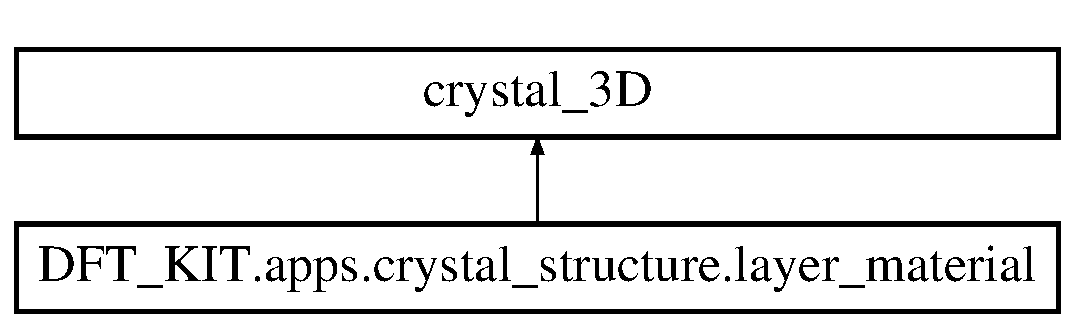
\includegraphics[height=2.000000cm]{class_d_f_t___k_i_t_1_1apps_1_1crystal__structure_1_1layer__material}
\end{center}
\end{figure}
\subsection*{Public Member Functions}
\begin{DoxyCompactItemize}
\item 
def \hyperlink{class_d_f_t___k_i_t_1_1apps_1_1crystal__structure_1_1layer__material_aa5565f9f818510781490e372734c5926}{\+\_\+\+\_\+init\+\_\+\+\_\+}
\end{DoxyCompactItemize}


\subsection{Detailed Description}


Definition at line 43 of file crystal\+\_\+structure.\+py.



\subsection{Constructor \& Destructor Documentation}
\hypertarget{class_d_f_t___k_i_t_1_1apps_1_1crystal__structure_1_1layer__material_aa5565f9f818510781490e372734c5926}{\index{D\+F\+T\+\_\+\+K\+I\+T\+::apps\+::crystal\+\_\+structure\+::layer\+\_\+material@{D\+F\+T\+\_\+\+K\+I\+T\+::apps\+::crystal\+\_\+structure\+::layer\+\_\+material}!\+\_\+\+\_\+init\+\_\+\+\_\+@{\+\_\+\+\_\+init\+\_\+\+\_\+}}
\index{\+\_\+\+\_\+init\+\_\+\+\_\+@{\+\_\+\+\_\+init\+\_\+\+\_\+}!D\+F\+T\+\_\+\+K\+I\+T\+::apps\+::crystal\+\_\+structure\+::layer\+\_\+material@{D\+F\+T\+\_\+\+K\+I\+T\+::apps\+::crystal\+\_\+structure\+::layer\+\_\+material}}
\subsubsection[{\+\_\+\+\_\+init\+\_\+\+\_\+}]{\setlength{\rightskip}{0pt plus 5cm}def D\+F\+T\+\_\+\+K\+I\+T.\+apps.\+crystal\+\_\+structure.\+layer\+\_\+material.\+\_\+\+\_\+init\+\_\+\+\_\+ (
\begin{DoxyParamCaption}
\item[{}]{self, }
\item[{}]{length\+\_\+unit = {\ttfamily 1.0}}
\end{DoxyParamCaption}
)}}\label{class_d_f_t___k_i_t_1_1apps_1_1crystal__structure_1_1layer__material_aa5565f9f818510781490e372734c5926}


Definition at line 44 of file crystal\+\_\+structure.\+py.



The documentation for this class was generated from the following file\+:\begin{DoxyCompactItemize}
\item 
apps/\hyperlink{crystal__structure_8py}{crystal\+\_\+structure.\+py}\end{DoxyCompactItemize}

\hypertarget{class_d_f_t___k_i_t_1_1core_1_1crystal__3_d_1_1monoclinic__3_d}{\section{D\+F\+T\+\_\+\+K\+I\+T.\+core.\+crystal\+\_\+3\+D.\+monoclinic\+\_\+3\+D Class Reference}
\label{class_d_f_t___k_i_t_1_1core_1_1crystal__3_d_1_1monoclinic__3_d}\index{D\+F\+T\+\_\+\+K\+I\+T.\+core.\+crystal\+\_\+3\+D.\+monoclinic\+\_\+3\+D@{D\+F\+T\+\_\+\+K\+I\+T.\+core.\+crystal\+\_\+3\+D.\+monoclinic\+\_\+3\+D}}
}
Inheritance diagram for D\+F\+T\+\_\+\+K\+I\+T.\+core.\+crystal\+\_\+3\+D.\+monoclinic\+\_\+3\+D\+:\begin{figure}[H]
\begin{center}
\leavevmode
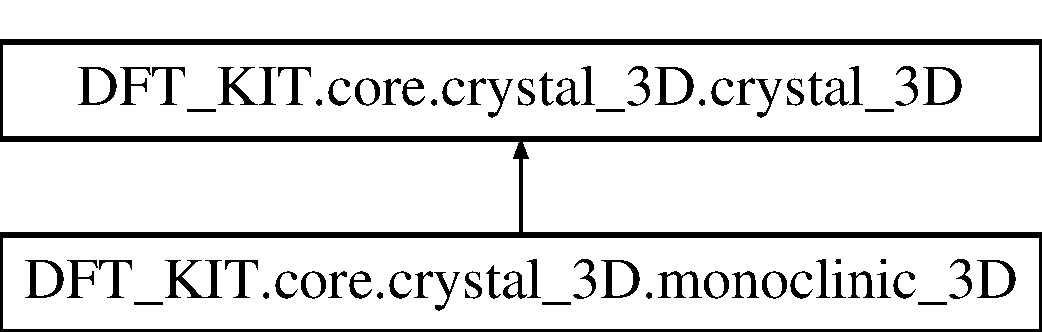
\includegraphics[height=2.000000cm]{class_d_f_t___k_i_t_1_1core_1_1crystal__3_d_1_1monoclinic__3_d}
\end{center}
\end{figure}
\subsection*{Public Member Functions}
\begin{DoxyCompactItemize}
\item 
def \hyperlink{class_d_f_t___k_i_t_1_1core_1_1crystal__3_d_1_1monoclinic__3_d_a44b4a6b8eb9ababeee422b1c2f7d16a3}{\+\_\+\+\_\+init\+\_\+\+\_\+}
\item 
def \hyperlink{class_d_f_t___k_i_t_1_1core_1_1crystal__3_d_1_1monoclinic__3_d_a718de9988bedf7b2b20de7362591e5c9}{set\+\_\+lattice}
\end{DoxyCompactItemize}
\subsection*{Additional Inherited Members}


\subsection{Detailed Description}


Definition at line 319 of file crystal\+\_\+3\+D.\+py.



\subsection{Constructor \& Destructor Documentation}
\hypertarget{class_d_f_t___k_i_t_1_1core_1_1crystal__3_d_1_1monoclinic__3_d_a44b4a6b8eb9ababeee422b1c2f7d16a3}{\index{D\+F\+T\+\_\+\+K\+I\+T\+::core\+::crystal\+\_\+3\+D\+::monoclinic\+\_\+3\+D@{D\+F\+T\+\_\+\+K\+I\+T\+::core\+::crystal\+\_\+3\+D\+::monoclinic\+\_\+3\+D}!\+\_\+\+\_\+init\+\_\+\+\_\+@{\+\_\+\+\_\+init\+\_\+\+\_\+}}
\index{\+\_\+\+\_\+init\+\_\+\+\_\+@{\+\_\+\+\_\+init\+\_\+\+\_\+}!D\+F\+T\+\_\+\+K\+I\+T\+::core\+::crystal\+\_\+3\+D\+::monoclinic\+\_\+3\+D@{D\+F\+T\+\_\+\+K\+I\+T\+::core\+::crystal\+\_\+3\+D\+::monoclinic\+\_\+3\+D}}
\subsubsection[{\+\_\+\+\_\+init\+\_\+\+\_\+}]{\setlength{\rightskip}{0pt plus 5cm}def D\+F\+T\+\_\+\+K\+I\+T.\+core.\+crystal\+\_\+3\+D.\+monoclinic\+\_\+3\+D.\+\_\+\+\_\+init\+\_\+\+\_\+ (
\begin{DoxyParamCaption}
\item[{}]{self, }
\item[{}]{a\+\_\+ = {\ttfamily 0.0}, }
\item[{}]{b\+\_\+ = {\ttfamily 0.0}, }
\item[{}]{c\+\_\+ = {\ttfamily 0.0}, }
\item[{}]{angle\+\_\+ = {\ttfamily 0.0}, }
\item[{}]{length\+\_\+unit = {\ttfamily 1.0}}
\end{DoxyParamCaption}
)}}\label{class_d_f_t___k_i_t_1_1core_1_1crystal__3_d_1_1monoclinic__3_d_a44b4a6b8eb9ababeee422b1c2f7d16a3}


Definition at line 320 of file crystal\+\_\+3\+D.\+py.



\subsection{Member Function Documentation}
\hypertarget{class_d_f_t___k_i_t_1_1core_1_1crystal__3_d_1_1monoclinic__3_d_a718de9988bedf7b2b20de7362591e5c9}{\index{D\+F\+T\+\_\+\+K\+I\+T\+::core\+::crystal\+\_\+3\+D\+::monoclinic\+\_\+3\+D@{D\+F\+T\+\_\+\+K\+I\+T\+::core\+::crystal\+\_\+3\+D\+::monoclinic\+\_\+3\+D}!set\+\_\+lattice@{set\+\_\+lattice}}
\index{set\+\_\+lattice@{set\+\_\+lattice}!D\+F\+T\+\_\+\+K\+I\+T\+::core\+::crystal\+\_\+3\+D\+::monoclinic\+\_\+3\+D@{D\+F\+T\+\_\+\+K\+I\+T\+::core\+::crystal\+\_\+3\+D\+::monoclinic\+\_\+3\+D}}
\subsubsection[{set\+\_\+lattice}]{\setlength{\rightskip}{0pt plus 5cm}def D\+F\+T\+\_\+\+K\+I\+T.\+core.\+crystal\+\_\+3\+D.\+monoclinic\+\_\+3\+D.\+set\+\_\+lattice (
\begin{DoxyParamCaption}
\item[{}]{self, }
\item[{}]{a\+\_\+, }
\item[{}]{b\+\_\+, }
\item[{}]{c\+\_\+, }
\item[{}]{angle\+\_\+}
\end{DoxyParamCaption}
)}}\label{class_d_f_t___k_i_t_1_1core_1_1crystal__3_d_1_1monoclinic__3_d_a718de9988bedf7b2b20de7362591e5c9}


Definition at line 324 of file crystal\+\_\+3\+D.\+py.



The documentation for this class was generated from the following file\+:\begin{DoxyCompactItemize}
\item 
core/\hyperlink{crystal__3_d_8py}{crystal\+\_\+3\+D.\+py}\end{DoxyCompactItemize}

\hypertarget{class_d_f_t___k_i_t_1_1core_1_1crystal__3_d_1_1orthorhombic__3_d}{\section{D\+F\+T\+\_\+\+K\+I\+T.\+core.\+crystal\+\_\+3\+D.\+orthorhombic\+\_\+3\+D Class Reference}
\label{class_d_f_t___k_i_t_1_1core_1_1crystal__3_d_1_1orthorhombic__3_d}\index{D\+F\+T\+\_\+\+K\+I\+T.\+core.\+crystal\+\_\+3\+D.\+orthorhombic\+\_\+3\+D@{D\+F\+T\+\_\+\+K\+I\+T.\+core.\+crystal\+\_\+3\+D.\+orthorhombic\+\_\+3\+D}}
}
Inheritance diagram for D\+F\+T\+\_\+\+K\+I\+T.\+core.\+crystal\+\_\+3\+D.\+orthorhombic\+\_\+3\+D\+:\begin{figure}[H]
\begin{center}
\leavevmode
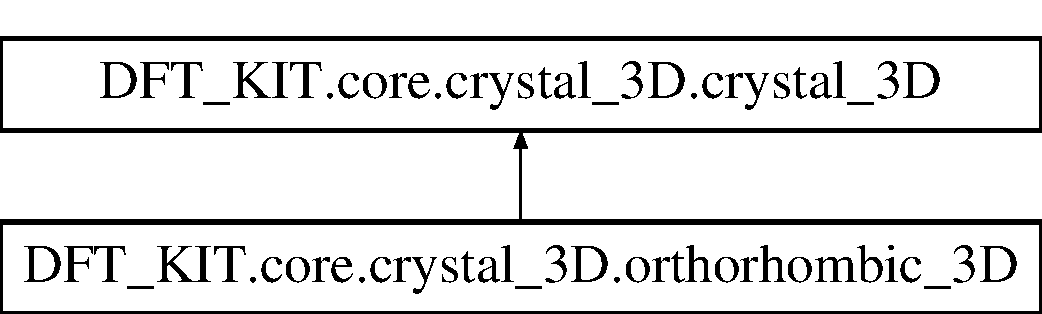
\includegraphics[height=2.000000cm]{class_d_f_t___k_i_t_1_1core_1_1crystal__3_d_1_1orthorhombic__3_d}
\end{center}
\end{figure}
\subsection*{Public Member Functions}
\begin{DoxyCompactItemize}
\item 
def \hyperlink{class_d_f_t___k_i_t_1_1core_1_1crystal__3_d_1_1orthorhombic__3_d_ac8aa417e23afd8497bdcbfd314788126}{\+\_\+\+\_\+init\+\_\+\+\_\+}
\item 
def \hyperlink{class_d_f_t___k_i_t_1_1core_1_1crystal__3_d_1_1orthorhombic__3_d_a9071af2f60daae5228990bf8ff73a49a}{set\+\_\+lattice}
\item 
def \hyperlink{class_d_f_t___k_i_t_1_1core_1_1crystal__3_d_1_1orthorhombic__3_d_a9697a1899c5f7368be6cdd2c25cf808d}{define\+\_\+klabels}
\end{DoxyCompactItemize}
\subsection*{Additional Inherited Members}


\subsection{Detailed Description}


Definition at line 284 of file crystal\+\_\+3\+D.\+py.



\subsection{Constructor \& Destructor Documentation}
\hypertarget{class_d_f_t___k_i_t_1_1core_1_1crystal__3_d_1_1orthorhombic__3_d_ac8aa417e23afd8497bdcbfd314788126}{\index{D\+F\+T\+\_\+\+K\+I\+T\+::core\+::crystal\+\_\+3\+D\+::orthorhombic\+\_\+3\+D@{D\+F\+T\+\_\+\+K\+I\+T\+::core\+::crystal\+\_\+3\+D\+::orthorhombic\+\_\+3\+D}!\+\_\+\+\_\+init\+\_\+\+\_\+@{\+\_\+\+\_\+init\+\_\+\+\_\+}}
\index{\+\_\+\+\_\+init\+\_\+\+\_\+@{\+\_\+\+\_\+init\+\_\+\+\_\+}!D\+F\+T\+\_\+\+K\+I\+T\+::core\+::crystal\+\_\+3\+D\+::orthorhombic\+\_\+3\+D@{D\+F\+T\+\_\+\+K\+I\+T\+::core\+::crystal\+\_\+3\+D\+::orthorhombic\+\_\+3\+D}}
\subsubsection[{\+\_\+\+\_\+init\+\_\+\+\_\+}]{\setlength{\rightskip}{0pt plus 5cm}def D\+F\+T\+\_\+\+K\+I\+T.\+core.\+crystal\+\_\+3\+D.\+orthorhombic\+\_\+3\+D.\+\_\+\+\_\+init\+\_\+\+\_\+ (
\begin{DoxyParamCaption}
\item[{}]{self, }
\item[{}]{a\+\_\+ = {\ttfamily 0.0}, }
\item[{}]{b\+\_\+ = {\ttfamily 0.0}, }
\item[{}]{c\+\_\+ = {\ttfamily 0.0}, }
\item[{}]{length\+\_\+unit = {\ttfamily 1.0}}
\end{DoxyParamCaption}
)}}\label{class_d_f_t___k_i_t_1_1core_1_1crystal__3_d_1_1orthorhombic__3_d_ac8aa417e23afd8497bdcbfd314788126}


Definition at line 285 of file crystal\+\_\+3\+D.\+py.



\subsection{Member Function Documentation}
\hypertarget{class_d_f_t___k_i_t_1_1core_1_1crystal__3_d_1_1orthorhombic__3_d_a9697a1899c5f7368be6cdd2c25cf808d}{\index{D\+F\+T\+\_\+\+K\+I\+T\+::core\+::crystal\+\_\+3\+D\+::orthorhombic\+\_\+3\+D@{D\+F\+T\+\_\+\+K\+I\+T\+::core\+::crystal\+\_\+3\+D\+::orthorhombic\+\_\+3\+D}!define\+\_\+klabels@{define\+\_\+klabels}}
\index{define\+\_\+klabels@{define\+\_\+klabels}!D\+F\+T\+\_\+\+K\+I\+T\+::core\+::crystal\+\_\+3\+D\+::orthorhombic\+\_\+3\+D@{D\+F\+T\+\_\+\+K\+I\+T\+::core\+::crystal\+\_\+3\+D\+::orthorhombic\+\_\+3\+D}}
\subsubsection[{define\+\_\+klabels}]{\setlength{\rightskip}{0pt plus 5cm}def D\+F\+T\+\_\+\+K\+I\+T.\+core.\+crystal\+\_\+3\+D.\+orthorhombic\+\_\+3\+D.\+define\+\_\+klabels (
\begin{DoxyParamCaption}
\item[{}]{self}
\end{DoxyParamCaption}
)}}\label{class_d_f_t___k_i_t_1_1core_1_1crystal__3_d_1_1orthorhombic__3_d_a9697a1899c5f7368be6cdd2c25cf808d}


Definition at line 296 of file crystal\+\_\+3\+D.\+py.

\hypertarget{class_d_f_t___k_i_t_1_1core_1_1crystal__3_d_1_1orthorhombic__3_d_a9071af2f60daae5228990bf8ff73a49a}{\index{D\+F\+T\+\_\+\+K\+I\+T\+::core\+::crystal\+\_\+3\+D\+::orthorhombic\+\_\+3\+D@{D\+F\+T\+\_\+\+K\+I\+T\+::core\+::crystal\+\_\+3\+D\+::orthorhombic\+\_\+3\+D}!set\+\_\+lattice@{set\+\_\+lattice}}
\index{set\+\_\+lattice@{set\+\_\+lattice}!D\+F\+T\+\_\+\+K\+I\+T\+::core\+::crystal\+\_\+3\+D\+::orthorhombic\+\_\+3\+D@{D\+F\+T\+\_\+\+K\+I\+T\+::core\+::crystal\+\_\+3\+D\+::orthorhombic\+\_\+3\+D}}
\subsubsection[{set\+\_\+lattice}]{\setlength{\rightskip}{0pt plus 5cm}def D\+F\+T\+\_\+\+K\+I\+T.\+core.\+crystal\+\_\+3\+D.\+orthorhombic\+\_\+3\+D.\+set\+\_\+lattice (
\begin{DoxyParamCaption}
\item[{}]{self, }
\item[{}]{a\+\_\+, }
\item[{}]{b\+\_\+, }
\item[{}]{c\+\_\+}
\end{DoxyParamCaption}
)}}\label{class_d_f_t___k_i_t_1_1core_1_1crystal__3_d_1_1orthorhombic__3_d_a9071af2f60daae5228990bf8ff73a49a}


Definition at line 290 of file crystal\+\_\+3\+D.\+py.



The documentation for this class was generated from the following file\+:\begin{DoxyCompactItemize}
\item 
core/\hyperlink{crystal__3_d_8py}{crystal\+\_\+3\+D.\+py}\end{DoxyCompactItemize}

\hypertarget{class_d_f_t___k_i_t_1_1apps_1_1crystal__structure_1_1perovskite}{\section{D\+F\+T\+\_\+\+K\+I\+T.\+apps.\+crystal\+\_\+structure.\+perovskite Class Reference}
\label{class_d_f_t___k_i_t_1_1apps_1_1crystal__structure_1_1perovskite}\index{D\+F\+T\+\_\+\+K\+I\+T.\+apps.\+crystal\+\_\+structure.\+perovskite@{D\+F\+T\+\_\+\+K\+I\+T.\+apps.\+crystal\+\_\+structure.\+perovskite}}
}
Inheritance diagram for D\+F\+T\+\_\+\+K\+I\+T.\+apps.\+crystal\+\_\+structure.\+perovskite\+:\begin{figure}[H]
\begin{center}
\leavevmode
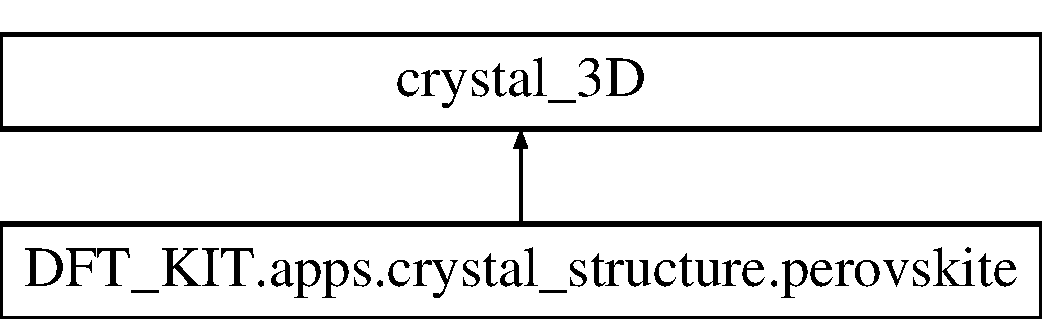
\includegraphics[height=2.000000cm]{class_d_f_t___k_i_t_1_1apps_1_1crystal__structure_1_1perovskite}
\end{center}
\end{figure}
\subsection*{Public Member Functions}
\begin{DoxyCompactItemize}
\item 
def \hyperlink{class_d_f_t___k_i_t_1_1apps_1_1crystal__structure_1_1perovskite_a8298df5110111a10afece4a7c4a0a87b}{\+\_\+\+\_\+init\+\_\+\+\_\+}
\end{DoxyCompactItemize}


\subsection{Detailed Description}


Definition at line 52 of file crystal\+\_\+structure.\+py.



\subsection{Constructor \& Destructor Documentation}
\hypertarget{class_d_f_t___k_i_t_1_1apps_1_1crystal__structure_1_1perovskite_a8298df5110111a10afece4a7c4a0a87b}{\index{D\+F\+T\+\_\+\+K\+I\+T\+::apps\+::crystal\+\_\+structure\+::perovskite@{D\+F\+T\+\_\+\+K\+I\+T\+::apps\+::crystal\+\_\+structure\+::perovskite}!\+\_\+\+\_\+init\+\_\+\+\_\+@{\+\_\+\+\_\+init\+\_\+\+\_\+}}
\index{\+\_\+\+\_\+init\+\_\+\+\_\+@{\+\_\+\+\_\+init\+\_\+\+\_\+}!D\+F\+T\+\_\+\+K\+I\+T\+::apps\+::crystal\+\_\+structure\+::perovskite@{D\+F\+T\+\_\+\+K\+I\+T\+::apps\+::crystal\+\_\+structure\+::perovskite}}
\subsubsection[{\+\_\+\+\_\+init\+\_\+\+\_\+}]{\setlength{\rightskip}{0pt plus 5cm}def D\+F\+T\+\_\+\+K\+I\+T.\+apps.\+crystal\+\_\+structure.\+perovskite.\+\_\+\+\_\+init\+\_\+\+\_\+ (
\begin{DoxyParamCaption}
\item[{}]{self, }
\item[{}]{length\+\_\+unit = {\ttfamily 1.0}}
\end{DoxyParamCaption}
)}}\label{class_d_f_t___k_i_t_1_1apps_1_1crystal__structure_1_1perovskite_a8298df5110111a10afece4a7c4a0a87b}


Definition at line 53 of file crystal\+\_\+structure.\+py.



The documentation for this class was generated from the following file\+:\begin{DoxyCompactItemize}
\item 
apps/\hyperlink{crystal__structure_8py}{crystal\+\_\+structure.\+py}\end{DoxyCompactItemize}

\hypertarget{class_d_f_t___k_i_t_1_1apps_1_1slab__surface__rhom_1_1_rhom__parallel__trigonal__surface}{\section{D\+F\+T\+\_\+\+K\+I\+T.\+apps.\+slab\+\_\+surface\+\_\+rhom.\+Rhom\+\_\+parallel\+\_\+trigonal\+\_\+surface Class Reference}
\label{class_d_f_t___k_i_t_1_1apps_1_1slab__surface__rhom_1_1_rhom__parallel__trigonal__surface}\index{D\+F\+T\+\_\+\+K\+I\+T.\+apps.\+slab\+\_\+surface\+\_\+rhom.\+Rhom\+\_\+parallel\+\_\+trigonal\+\_\+surface@{D\+F\+T\+\_\+\+K\+I\+T.\+apps.\+slab\+\_\+surface\+\_\+rhom.\+Rhom\+\_\+parallel\+\_\+trigonal\+\_\+surface}}
}
Inheritance diagram for D\+F\+T\+\_\+\+K\+I\+T.\+apps.\+slab\+\_\+surface\+\_\+rhom.\+Rhom\+\_\+parallel\+\_\+trigonal\+\_\+surface\+:\begin{figure}[H]
\begin{center}
\leavevmode
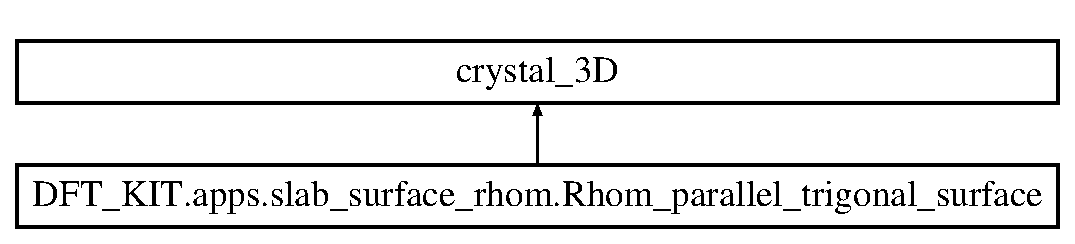
\includegraphics[height=2.000000cm]{class_d_f_t___k_i_t_1_1apps_1_1slab__surface__rhom_1_1_rhom__parallel__trigonal__surface}
\end{center}
\end{figure}
\subsection*{Public Member Functions}
\begin{DoxyCompactItemize}
\item 
def \hyperlink{class_d_f_t___k_i_t_1_1apps_1_1slab__surface__rhom_1_1_rhom__parallel__trigonal__surface_ab4aa2dd9eefafe4896d4b053ffc91bc2}{\+\_\+\+\_\+init\+\_\+\+\_\+}
\end{DoxyCompactItemize}
\subsection*{Public Attributes}
\begin{DoxyCompactItemize}
\item 
\hyperlink{class_d_f_t___k_i_t_1_1apps_1_1slab__surface__rhom_1_1_rhom__parallel__trigonal__surface_a42ef9900bdc7c47e6a52f6a5fed01e94}{ref\+\_\+crystal}
\end{DoxyCompactItemize}


\subsection{Detailed Description}


Definition at line 59 of file slab\+\_\+surface\+\_\+rhom.\+py.



\subsection{Constructor \& Destructor Documentation}
\hypertarget{class_d_f_t___k_i_t_1_1apps_1_1slab__surface__rhom_1_1_rhom__parallel__trigonal__surface_ab4aa2dd9eefafe4896d4b053ffc91bc2}{\index{D\+F\+T\+\_\+\+K\+I\+T\+::apps\+::slab\+\_\+surface\+\_\+rhom\+::\+Rhom\+\_\+parallel\+\_\+trigonal\+\_\+surface@{D\+F\+T\+\_\+\+K\+I\+T\+::apps\+::slab\+\_\+surface\+\_\+rhom\+::\+Rhom\+\_\+parallel\+\_\+trigonal\+\_\+surface}!\+\_\+\+\_\+init\+\_\+\+\_\+@{\+\_\+\+\_\+init\+\_\+\+\_\+}}
\index{\+\_\+\+\_\+init\+\_\+\+\_\+@{\+\_\+\+\_\+init\+\_\+\+\_\+}!D\+F\+T\+\_\+\+K\+I\+T\+::apps\+::slab\+\_\+surface\+\_\+rhom\+::\+Rhom\+\_\+parallel\+\_\+trigonal\+\_\+surface@{D\+F\+T\+\_\+\+K\+I\+T\+::apps\+::slab\+\_\+surface\+\_\+rhom\+::\+Rhom\+\_\+parallel\+\_\+trigonal\+\_\+surface}}
\subsubsection[{\+\_\+\+\_\+init\+\_\+\+\_\+}]{\setlength{\rightskip}{0pt plus 5cm}def D\+F\+T\+\_\+\+K\+I\+T.\+apps.\+slab\+\_\+surface\+\_\+rhom.\+Rhom\+\_\+parallel\+\_\+trigonal\+\_\+surface.\+\_\+\+\_\+init\+\_\+\+\_\+ (
\begin{DoxyParamCaption}
\item[{}]{self, }
\item[{}]{element, }
\item[{}]{num\+\_\+layers, }
\item[{}]{vacuum\+\_\+layers, }
\item[{}]{length\+\_\+unit = {\ttfamily 1.0}, }
\item[{}]{description = {\ttfamily 'Trigonal~Surface'}, }
\item[{}]{parms}
\end{DoxyParamCaption}
)}}\label{class_d_f_t___k_i_t_1_1apps_1_1slab__surface__rhom_1_1_rhom__parallel__trigonal__surface_ab4aa2dd9eefafe4896d4b053ffc91bc2}


Definition at line 60 of file slab\+\_\+surface\+\_\+rhom.\+py.



\subsection{Member Data Documentation}
\hypertarget{class_d_f_t___k_i_t_1_1apps_1_1slab__surface__rhom_1_1_rhom__parallel__trigonal__surface_a42ef9900bdc7c47e6a52f6a5fed01e94}{\index{D\+F\+T\+\_\+\+K\+I\+T\+::apps\+::slab\+\_\+surface\+\_\+rhom\+::\+Rhom\+\_\+parallel\+\_\+trigonal\+\_\+surface@{D\+F\+T\+\_\+\+K\+I\+T\+::apps\+::slab\+\_\+surface\+\_\+rhom\+::\+Rhom\+\_\+parallel\+\_\+trigonal\+\_\+surface}!ref\+\_\+crystal@{ref\+\_\+crystal}}
\index{ref\+\_\+crystal@{ref\+\_\+crystal}!D\+F\+T\+\_\+\+K\+I\+T\+::apps\+::slab\+\_\+surface\+\_\+rhom\+::\+Rhom\+\_\+parallel\+\_\+trigonal\+\_\+surface@{D\+F\+T\+\_\+\+K\+I\+T\+::apps\+::slab\+\_\+surface\+\_\+rhom\+::\+Rhom\+\_\+parallel\+\_\+trigonal\+\_\+surface}}
\subsubsection[{ref\+\_\+crystal}]{\setlength{\rightskip}{0pt plus 5cm}D\+F\+T\+\_\+\+K\+I\+T.\+apps.\+slab\+\_\+surface\+\_\+rhom.\+Rhom\+\_\+parallel\+\_\+trigonal\+\_\+surface.\+ref\+\_\+crystal}}\label{class_d_f_t___k_i_t_1_1apps_1_1slab__surface__rhom_1_1_rhom__parallel__trigonal__surface_a42ef9900bdc7c47e6a52f6a5fed01e94}


Definition at line 77 of file slab\+\_\+surface\+\_\+rhom.\+py.



The documentation for this class was generated from the following file\+:\begin{DoxyCompactItemize}
\item 
apps/\hyperlink{slab__surface__rhom_8py}{slab\+\_\+surface\+\_\+rhom.\+py}\end{DoxyCompactItemize}

\hypertarget{class_d_f_t___k_i_t_1_1apps_1_1wire__rhom_1_1_rhom__trigonal__nanowire}{\section{D\+F\+T\+\_\+\+K\+I\+T.\+apps.\+wire\+\_\+rhom.\+Rhom\+\_\+trigonal\+\_\+nanowire Class Reference}
\label{class_d_f_t___k_i_t_1_1apps_1_1wire__rhom_1_1_rhom__trigonal__nanowire}\index{D\+F\+T\+\_\+\+K\+I\+T.\+apps.\+wire\+\_\+rhom.\+Rhom\+\_\+trigonal\+\_\+nanowire@{D\+F\+T\+\_\+\+K\+I\+T.\+apps.\+wire\+\_\+rhom.\+Rhom\+\_\+trigonal\+\_\+nanowire}}
}
Inheritance diagram for D\+F\+T\+\_\+\+K\+I\+T.\+apps.\+wire\+\_\+rhom.\+Rhom\+\_\+trigonal\+\_\+nanowire\+:\begin{figure}[H]
\begin{center}
\leavevmode
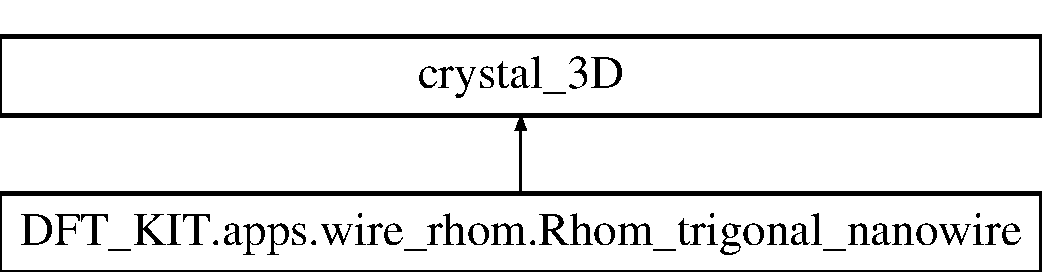
\includegraphics[height=2.000000cm]{class_d_f_t___k_i_t_1_1apps_1_1wire__rhom_1_1_rhom__trigonal__nanowire}
\end{center}
\end{figure}
\subsection*{Public Member Functions}
\begin{DoxyCompactItemize}
\item 
def \hyperlink{class_d_f_t___k_i_t_1_1apps_1_1wire__rhom_1_1_rhom__trigonal__nanowire_a74bcdd04bf4048cfefb5be83f7f15fe2}{\+\_\+\+\_\+init\+\_\+\+\_\+}
\end{DoxyCompactItemize}
\subsection*{Public Attributes}
\begin{DoxyCompactItemize}
\item 
\hyperlink{class_d_f_t___k_i_t_1_1apps_1_1wire__rhom_1_1_rhom__trigonal__nanowire_a24be6451c8eea10c855b4894e7319e82}{ref\+\_\+crystal}
\item 
\hyperlink{class_d_f_t___k_i_t_1_1apps_1_1wire__rhom_1_1_rhom__trigonal__nanowire_a342afa8a5416b188a5938b0572c2abf9}{Lx}
\item 
\hyperlink{class_d_f_t___k_i_t_1_1apps_1_1wire__rhom_1_1_rhom__trigonal__nanowire_a5e4b1d53b0fd2aa4f6d3f0f51b1b182c}{Ly}
\item 
\hyperlink{class_d_f_t___k_i_t_1_1apps_1_1wire__rhom_1_1_rhom__trigonal__nanowire_a87a9ce98f3c0724d7ffd9cf4562262fc}{Lz}
\item 
\hyperlink{class_d_f_t___k_i_t_1_1apps_1_1wire__rhom_1_1_rhom__trigonal__nanowire_ad2f62d13d4541e9c45097aa8bd084fd6}{radius}
\item 
\hyperlink{class_d_f_t___k_i_t_1_1apps_1_1wire__rhom_1_1_rhom__trigonal__nanowire_aa1495a694e9e0414219f8821c03c9cd4}{hex\+\_\+a1}
\item 
\hyperlink{class_d_f_t___k_i_t_1_1apps_1_1wire__rhom_1_1_rhom__trigonal__nanowire_aab46e89964027acc5ade4a9a0138db4e}{hex\+\_\+a2}
\item 
\hyperlink{class_d_f_t___k_i_t_1_1apps_1_1wire__rhom_1_1_rhom__trigonal__nanowire_a7d2b3c313795b90d803abe40abee80d9}{all\+\_\+points}
\end{DoxyCompactItemize}


\subsection{Detailed Description}


Definition at line 12 of file wire\+\_\+rhom.\+py.



\subsection{Constructor \& Destructor Documentation}
\hypertarget{class_d_f_t___k_i_t_1_1apps_1_1wire__rhom_1_1_rhom__trigonal__nanowire_a74bcdd04bf4048cfefb5be83f7f15fe2}{\index{D\+F\+T\+\_\+\+K\+I\+T\+::apps\+::wire\+\_\+rhom\+::\+Rhom\+\_\+trigonal\+\_\+nanowire@{D\+F\+T\+\_\+\+K\+I\+T\+::apps\+::wire\+\_\+rhom\+::\+Rhom\+\_\+trigonal\+\_\+nanowire}!\+\_\+\+\_\+init\+\_\+\+\_\+@{\+\_\+\+\_\+init\+\_\+\+\_\+}}
\index{\+\_\+\+\_\+init\+\_\+\+\_\+@{\+\_\+\+\_\+init\+\_\+\+\_\+}!D\+F\+T\+\_\+\+K\+I\+T\+::apps\+::wire\+\_\+rhom\+::\+Rhom\+\_\+trigonal\+\_\+nanowire@{D\+F\+T\+\_\+\+K\+I\+T\+::apps\+::wire\+\_\+rhom\+::\+Rhom\+\_\+trigonal\+\_\+nanowire}}
\subsubsection[{\+\_\+\+\_\+init\+\_\+\+\_\+}]{\setlength{\rightskip}{0pt plus 5cm}def D\+F\+T\+\_\+\+K\+I\+T.\+apps.\+wire\+\_\+rhom.\+Rhom\+\_\+trigonal\+\_\+nanowire.\+\_\+\+\_\+init\+\_\+\+\_\+ (
\begin{DoxyParamCaption}
\item[{}]{self, }
\item[{}]{element, }
\item[{}]{Lx, }
\item[{}]{Ly, }
\item[{}]{radius, }
\item[{}]{length\+\_\+unit = {\ttfamily 1.0}, }
\item[{}]{description = {\ttfamily 'Trigonal~Nanowire'}, }
\item[{}]{parms}
\end{DoxyParamCaption}
)}}\label{class_d_f_t___k_i_t_1_1apps_1_1wire__rhom_1_1_rhom__trigonal__nanowire_a74bcdd04bf4048cfefb5be83f7f15fe2}


Definition at line 13 of file wire\+\_\+rhom.\+py.



\subsection{Member Data Documentation}
\hypertarget{class_d_f_t___k_i_t_1_1apps_1_1wire__rhom_1_1_rhom__trigonal__nanowire_a7d2b3c313795b90d803abe40abee80d9}{\index{D\+F\+T\+\_\+\+K\+I\+T\+::apps\+::wire\+\_\+rhom\+::\+Rhom\+\_\+trigonal\+\_\+nanowire@{D\+F\+T\+\_\+\+K\+I\+T\+::apps\+::wire\+\_\+rhom\+::\+Rhom\+\_\+trigonal\+\_\+nanowire}!all\+\_\+points@{all\+\_\+points}}
\index{all\+\_\+points@{all\+\_\+points}!D\+F\+T\+\_\+\+K\+I\+T\+::apps\+::wire\+\_\+rhom\+::\+Rhom\+\_\+trigonal\+\_\+nanowire@{D\+F\+T\+\_\+\+K\+I\+T\+::apps\+::wire\+\_\+rhom\+::\+Rhom\+\_\+trigonal\+\_\+nanowire}}
\subsubsection[{all\+\_\+points}]{\setlength{\rightskip}{0pt plus 5cm}D\+F\+T\+\_\+\+K\+I\+T.\+apps.\+wire\+\_\+rhom.\+Rhom\+\_\+trigonal\+\_\+nanowire.\+all\+\_\+points}}\label{class_d_f_t___k_i_t_1_1apps_1_1wire__rhom_1_1_rhom__trigonal__nanowire_a7d2b3c313795b90d803abe40abee80d9}


Definition at line 106 of file wire\+\_\+rhom.\+py.

\hypertarget{class_d_f_t___k_i_t_1_1apps_1_1wire__rhom_1_1_rhom__trigonal__nanowire_aa1495a694e9e0414219f8821c03c9cd4}{\index{D\+F\+T\+\_\+\+K\+I\+T\+::apps\+::wire\+\_\+rhom\+::\+Rhom\+\_\+trigonal\+\_\+nanowire@{D\+F\+T\+\_\+\+K\+I\+T\+::apps\+::wire\+\_\+rhom\+::\+Rhom\+\_\+trigonal\+\_\+nanowire}!hex\+\_\+a1@{hex\+\_\+a1}}
\index{hex\+\_\+a1@{hex\+\_\+a1}!D\+F\+T\+\_\+\+K\+I\+T\+::apps\+::wire\+\_\+rhom\+::\+Rhom\+\_\+trigonal\+\_\+nanowire@{D\+F\+T\+\_\+\+K\+I\+T\+::apps\+::wire\+\_\+rhom\+::\+Rhom\+\_\+trigonal\+\_\+nanowire}}
\subsubsection[{hex\+\_\+a1}]{\setlength{\rightskip}{0pt plus 5cm}D\+F\+T\+\_\+\+K\+I\+T.\+apps.\+wire\+\_\+rhom.\+Rhom\+\_\+trigonal\+\_\+nanowire.\+hex\+\_\+a1}}\label{class_d_f_t___k_i_t_1_1apps_1_1wire__rhom_1_1_rhom__trigonal__nanowire_aa1495a694e9e0414219f8821c03c9cd4}


Definition at line 60 of file wire\+\_\+rhom.\+py.

\hypertarget{class_d_f_t___k_i_t_1_1apps_1_1wire__rhom_1_1_rhom__trigonal__nanowire_aab46e89964027acc5ade4a9a0138db4e}{\index{D\+F\+T\+\_\+\+K\+I\+T\+::apps\+::wire\+\_\+rhom\+::\+Rhom\+\_\+trigonal\+\_\+nanowire@{D\+F\+T\+\_\+\+K\+I\+T\+::apps\+::wire\+\_\+rhom\+::\+Rhom\+\_\+trigonal\+\_\+nanowire}!hex\+\_\+a2@{hex\+\_\+a2}}
\index{hex\+\_\+a2@{hex\+\_\+a2}!D\+F\+T\+\_\+\+K\+I\+T\+::apps\+::wire\+\_\+rhom\+::\+Rhom\+\_\+trigonal\+\_\+nanowire@{D\+F\+T\+\_\+\+K\+I\+T\+::apps\+::wire\+\_\+rhom\+::\+Rhom\+\_\+trigonal\+\_\+nanowire}}
\subsubsection[{hex\+\_\+a2}]{\setlength{\rightskip}{0pt plus 5cm}D\+F\+T\+\_\+\+K\+I\+T.\+apps.\+wire\+\_\+rhom.\+Rhom\+\_\+trigonal\+\_\+nanowire.\+hex\+\_\+a2}}\label{class_d_f_t___k_i_t_1_1apps_1_1wire__rhom_1_1_rhom__trigonal__nanowire_aab46e89964027acc5ade4a9a0138db4e}


Definition at line 61 of file wire\+\_\+rhom.\+py.

\hypertarget{class_d_f_t___k_i_t_1_1apps_1_1wire__rhom_1_1_rhom__trigonal__nanowire_a342afa8a5416b188a5938b0572c2abf9}{\index{D\+F\+T\+\_\+\+K\+I\+T\+::apps\+::wire\+\_\+rhom\+::\+Rhom\+\_\+trigonal\+\_\+nanowire@{D\+F\+T\+\_\+\+K\+I\+T\+::apps\+::wire\+\_\+rhom\+::\+Rhom\+\_\+trigonal\+\_\+nanowire}!Lx@{Lx}}
\index{Lx@{Lx}!D\+F\+T\+\_\+\+K\+I\+T\+::apps\+::wire\+\_\+rhom\+::\+Rhom\+\_\+trigonal\+\_\+nanowire@{D\+F\+T\+\_\+\+K\+I\+T\+::apps\+::wire\+\_\+rhom\+::\+Rhom\+\_\+trigonal\+\_\+nanowire}}
\subsubsection[{Lx}]{\setlength{\rightskip}{0pt plus 5cm}D\+F\+T\+\_\+\+K\+I\+T.\+apps.\+wire\+\_\+rhom.\+Rhom\+\_\+trigonal\+\_\+nanowire.\+Lx}}\label{class_d_f_t___k_i_t_1_1apps_1_1wire__rhom_1_1_rhom__trigonal__nanowire_a342afa8a5416b188a5938b0572c2abf9}


Definition at line 46 of file wire\+\_\+rhom.\+py.

\hypertarget{class_d_f_t___k_i_t_1_1apps_1_1wire__rhom_1_1_rhom__trigonal__nanowire_a5e4b1d53b0fd2aa4f6d3f0f51b1b182c}{\index{D\+F\+T\+\_\+\+K\+I\+T\+::apps\+::wire\+\_\+rhom\+::\+Rhom\+\_\+trigonal\+\_\+nanowire@{D\+F\+T\+\_\+\+K\+I\+T\+::apps\+::wire\+\_\+rhom\+::\+Rhom\+\_\+trigonal\+\_\+nanowire}!Ly@{Ly}}
\index{Ly@{Ly}!D\+F\+T\+\_\+\+K\+I\+T\+::apps\+::wire\+\_\+rhom\+::\+Rhom\+\_\+trigonal\+\_\+nanowire@{D\+F\+T\+\_\+\+K\+I\+T\+::apps\+::wire\+\_\+rhom\+::\+Rhom\+\_\+trigonal\+\_\+nanowire}}
\subsubsection[{Ly}]{\setlength{\rightskip}{0pt plus 5cm}D\+F\+T\+\_\+\+K\+I\+T.\+apps.\+wire\+\_\+rhom.\+Rhom\+\_\+trigonal\+\_\+nanowire.\+Ly}}\label{class_d_f_t___k_i_t_1_1apps_1_1wire__rhom_1_1_rhom__trigonal__nanowire_a5e4b1d53b0fd2aa4f6d3f0f51b1b182c}


Definition at line 47 of file wire\+\_\+rhom.\+py.

\hypertarget{class_d_f_t___k_i_t_1_1apps_1_1wire__rhom_1_1_rhom__trigonal__nanowire_a87a9ce98f3c0724d7ffd9cf4562262fc}{\index{D\+F\+T\+\_\+\+K\+I\+T\+::apps\+::wire\+\_\+rhom\+::\+Rhom\+\_\+trigonal\+\_\+nanowire@{D\+F\+T\+\_\+\+K\+I\+T\+::apps\+::wire\+\_\+rhom\+::\+Rhom\+\_\+trigonal\+\_\+nanowire}!Lz@{Lz}}
\index{Lz@{Lz}!D\+F\+T\+\_\+\+K\+I\+T\+::apps\+::wire\+\_\+rhom\+::\+Rhom\+\_\+trigonal\+\_\+nanowire@{D\+F\+T\+\_\+\+K\+I\+T\+::apps\+::wire\+\_\+rhom\+::\+Rhom\+\_\+trigonal\+\_\+nanowire}}
\subsubsection[{Lz}]{\setlength{\rightskip}{0pt plus 5cm}D\+F\+T\+\_\+\+K\+I\+T.\+apps.\+wire\+\_\+rhom.\+Rhom\+\_\+trigonal\+\_\+nanowire.\+Lz}}\label{class_d_f_t___k_i_t_1_1apps_1_1wire__rhom_1_1_rhom__trigonal__nanowire_a87a9ce98f3c0724d7ffd9cf4562262fc}


Definition at line 48 of file wire\+\_\+rhom.\+py.

\hypertarget{class_d_f_t___k_i_t_1_1apps_1_1wire__rhom_1_1_rhom__trigonal__nanowire_ad2f62d13d4541e9c45097aa8bd084fd6}{\index{D\+F\+T\+\_\+\+K\+I\+T\+::apps\+::wire\+\_\+rhom\+::\+Rhom\+\_\+trigonal\+\_\+nanowire@{D\+F\+T\+\_\+\+K\+I\+T\+::apps\+::wire\+\_\+rhom\+::\+Rhom\+\_\+trigonal\+\_\+nanowire}!radius@{radius}}
\index{radius@{radius}!D\+F\+T\+\_\+\+K\+I\+T\+::apps\+::wire\+\_\+rhom\+::\+Rhom\+\_\+trigonal\+\_\+nanowire@{D\+F\+T\+\_\+\+K\+I\+T\+::apps\+::wire\+\_\+rhom\+::\+Rhom\+\_\+trigonal\+\_\+nanowire}}
\subsubsection[{radius}]{\setlength{\rightskip}{0pt plus 5cm}D\+F\+T\+\_\+\+K\+I\+T.\+apps.\+wire\+\_\+rhom.\+Rhom\+\_\+trigonal\+\_\+nanowire.\+radius}}\label{class_d_f_t___k_i_t_1_1apps_1_1wire__rhom_1_1_rhom__trigonal__nanowire_ad2f62d13d4541e9c45097aa8bd084fd6}


Definition at line 49 of file wire\+\_\+rhom.\+py.

\hypertarget{class_d_f_t___k_i_t_1_1apps_1_1wire__rhom_1_1_rhom__trigonal__nanowire_a24be6451c8eea10c855b4894e7319e82}{\index{D\+F\+T\+\_\+\+K\+I\+T\+::apps\+::wire\+\_\+rhom\+::\+Rhom\+\_\+trigonal\+\_\+nanowire@{D\+F\+T\+\_\+\+K\+I\+T\+::apps\+::wire\+\_\+rhom\+::\+Rhom\+\_\+trigonal\+\_\+nanowire}!ref\+\_\+crystal@{ref\+\_\+crystal}}
\index{ref\+\_\+crystal@{ref\+\_\+crystal}!D\+F\+T\+\_\+\+K\+I\+T\+::apps\+::wire\+\_\+rhom\+::\+Rhom\+\_\+trigonal\+\_\+nanowire@{D\+F\+T\+\_\+\+K\+I\+T\+::apps\+::wire\+\_\+rhom\+::\+Rhom\+\_\+trigonal\+\_\+nanowire}}
\subsubsection[{ref\+\_\+crystal}]{\setlength{\rightskip}{0pt plus 5cm}D\+F\+T\+\_\+\+K\+I\+T.\+apps.\+wire\+\_\+rhom.\+Rhom\+\_\+trigonal\+\_\+nanowire.\+ref\+\_\+crystal}}\label{class_d_f_t___k_i_t_1_1apps_1_1wire__rhom_1_1_rhom__trigonal__nanowire_a24be6451c8eea10c855b4894e7319e82}


Definition at line 36 of file wire\+\_\+rhom.\+py.



The documentation for this class was generated from the following file\+:\begin{DoxyCompactItemize}
\item 
apps/\hyperlink{wire__rhom_8py}{wire\+\_\+rhom.\+py}\end{DoxyCompactItemize}

\hypertarget{class_d_f_t___k_i_t_1_1apps_1_1slab__surface__rhom_1_1_rhom__trigonal__surface}{\section{D\+F\+T\+\_\+\+K\+I\+T.\+apps.\+slab\+\_\+surface\+\_\+rhom.\+Rhom\+\_\+trigonal\+\_\+surface Class Reference}
\label{class_d_f_t___k_i_t_1_1apps_1_1slab__surface__rhom_1_1_rhom__trigonal__surface}\index{D\+F\+T\+\_\+\+K\+I\+T.\+apps.\+slab\+\_\+surface\+\_\+rhom.\+Rhom\+\_\+trigonal\+\_\+surface@{D\+F\+T\+\_\+\+K\+I\+T.\+apps.\+slab\+\_\+surface\+\_\+rhom.\+Rhom\+\_\+trigonal\+\_\+surface}}
}
Inheritance diagram for D\+F\+T\+\_\+\+K\+I\+T.\+apps.\+slab\+\_\+surface\+\_\+rhom.\+Rhom\+\_\+trigonal\+\_\+surface\+:\begin{figure}[H]
\begin{center}
\leavevmode
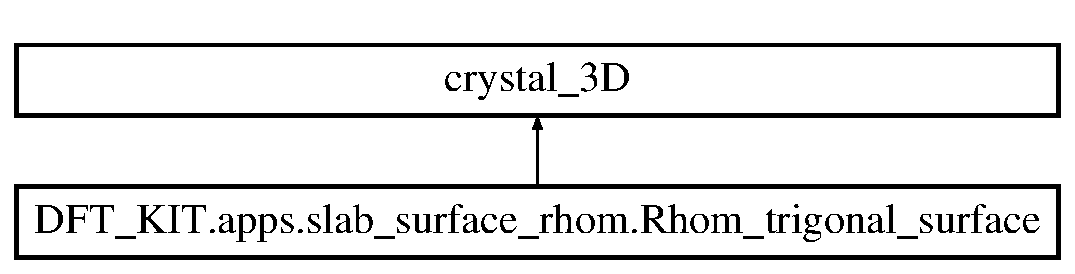
\includegraphics[height=2.000000cm]{class_d_f_t___k_i_t_1_1apps_1_1slab__surface__rhom_1_1_rhom__trigonal__surface}
\end{center}
\end{figure}
\subsection*{Public Member Functions}
\begin{DoxyCompactItemize}
\item 
def \hyperlink{class_d_f_t___k_i_t_1_1apps_1_1slab__surface__rhom_1_1_rhom__trigonal__surface_a4cf46ad804d400f760f89fccead8aa3f}{\+\_\+\+\_\+init\+\_\+\+\_\+}
\end{DoxyCompactItemize}
\subsection*{Public Attributes}
\begin{DoxyCompactItemize}
\item 
\hyperlink{class_d_f_t___k_i_t_1_1apps_1_1slab__surface__rhom_1_1_rhom__trigonal__surface_ac8b802d45e21f6b25c3830f69d586af0}{ref\+\_\+crystal}
\item 
\hyperlink{class_d_f_t___k_i_t_1_1apps_1_1slab__surface__rhom_1_1_rhom__trigonal__surface_a3dfbfe8019a222c410f028cda617c09c}{num\+\_\+layers}
\item 
\hyperlink{class_d_f_t___k_i_t_1_1apps_1_1slab__surface__rhom_1_1_rhom__trigonal__surface_ab595b72d6f93bce6ce61d31610cc882e}{vacuum\+\_\+layers}
\item 
\hyperlink{class_d_f_t___k_i_t_1_1apps_1_1slab__surface__rhom_1_1_rhom__trigonal__surface_ad09e487f3439b81b81e1b04b2aece740}{rhom\+\_\+constant}
\item 
\hyperlink{class_d_f_t___k_i_t_1_1apps_1_1slab__surface__rhom_1_1_rhom__trigonal__surface_adb18e885bfdfd9e77a3ae7cb783b405f}{angle}
\item 
\hyperlink{class_d_f_t___k_i_t_1_1apps_1_1slab__surface__rhom_1_1_rhom__trigonal__surface_ace9262e8227a0f6d26b7c9f422bd78a7}{rhom\+\_\+u}
\end{DoxyCompactItemize}


\subsection{Detailed Description}


Definition at line 9 of file slab\+\_\+surface\+\_\+rhom.\+py.



\subsection{Constructor \& Destructor Documentation}
\hypertarget{class_d_f_t___k_i_t_1_1apps_1_1slab__surface__rhom_1_1_rhom__trigonal__surface_a4cf46ad804d400f760f89fccead8aa3f}{\index{D\+F\+T\+\_\+\+K\+I\+T\+::apps\+::slab\+\_\+surface\+\_\+rhom\+::\+Rhom\+\_\+trigonal\+\_\+surface@{D\+F\+T\+\_\+\+K\+I\+T\+::apps\+::slab\+\_\+surface\+\_\+rhom\+::\+Rhom\+\_\+trigonal\+\_\+surface}!\+\_\+\+\_\+init\+\_\+\+\_\+@{\+\_\+\+\_\+init\+\_\+\+\_\+}}
\index{\+\_\+\+\_\+init\+\_\+\+\_\+@{\+\_\+\+\_\+init\+\_\+\+\_\+}!D\+F\+T\+\_\+\+K\+I\+T\+::apps\+::slab\+\_\+surface\+\_\+rhom\+::\+Rhom\+\_\+trigonal\+\_\+surface@{D\+F\+T\+\_\+\+K\+I\+T\+::apps\+::slab\+\_\+surface\+\_\+rhom\+::\+Rhom\+\_\+trigonal\+\_\+surface}}
\subsubsection[{\+\_\+\+\_\+init\+\_\+\+\_\+}]{\setlength{\rightskip}{0pt plus 5cm}def D\+F\+T\+\_\+\+K\+I\+T.\+apps.\+slab\+\_\+surface\+\_\+rhom.\+Rhom\+\_\+trigonal\+\_\+surface.\+\_\+\+\_\+init\+\_\+\+\_\+ (
\begin{DoxyParamCaption}
\item[{}]{self, }
\item[{}]{element, }
\item[{}]{num\+\_\+layers, }
\item[{}]{vacuum\+\_\+layers, }
\item[{}]{length\+\_\+unit = {\ttfamily 1.0}, }
\item[{}]{description = {\ttfamily 'Trigonal~Surface'}, }
\item[{}]{parms}
\end{DoxyParamCaption}
)}}\label{class_d_f_t___k_i_t_1_1apps_1_1slab__surface__rhom_1_1_rhom__trigonal__surface_a4cf46ad804d400f760f89fccead8aa3f}


Definition at line 10 of file slab\+\_\+surface\+\_\+rhom.\+py.



\subsection{Member Data Documentation}
\hypertarget{class_d_f_t___k_i_t_1_1apps_1_1slab__surface__rhom_1_1_rhom__trigonal__surface_adb18e885bfdfd9e77a3ae7cb783b405f}{\index{D\+F\+T\+\_\+\+K\+I\+T\+::apps\+::slab\+\_\+surface\+\_\+rhom\+::\+Rhom\+\_\+trigonal\+\_\+surface@{D\+F\+T\+\_\+\+K\+I\+T\+::apps\+::slab\+\_\+surface\+\_\+rhom\+::\+Rhom\+\_\+trigonal\+\_\+surface}!angle@{angle}}
\index{angle@{angle}!D\+F\+T\+\_\+\+K\+I\+T\+::apps\+::slab\+\_\+surface\+\_\+rhom\+::\+Rhom\+\_\+trigonal\+\_\+surface@{D\+F\+T\+\_\+\+K\+I\+T\+::apps\+::slab\+\_\+surface\+\_\+rhom\+::\+Rhom\+\_\+trigonal\+\_\+surface}}
\subsubsection[{angle}]{\setlength{\rightskip}{0pt plus 5cm}D\+F\+T\+\_\+\+K\+I\+T.\+apps.\+slab\+\_\+surface\+\_\+rhom.\+Rhom\+\_\+trigonal\+\_\+surface.\+angle}}\label{class_d_f_t___k_i_t_1_1apps_1_1slab__surface__rhom_1_1_rhom__trigonal__surface_adb18e885bfdfd9e77a3ae7cb783b405f}


Definition at line 36 of file slab\+\_\+surface\+\_\+rhom.\+py.

\hypertarget{class_d_f_t___k_i_t_1_1apps_1_1slab__surface__rhom_1_1_rhom__trigonal__surface_a3dfbfe8019a222c410f028cda617c09c}{\index{D\+F\+T\+\_\+\+K\+I\+T\+::apps\+::slab\+\_\+surface\+\_\+rhom\+::\+Rhom\+\_\+trigonal\+\_\+surface@{D\+F\+T\+\_\+\+K\+I\+T\+::apps\+::slab\+\_\+surface\+\_\+rhom\+::\+Rhom\+\_\+trigonal\+\_\+surface}!num\+\_\+layers@{num\+\_\+layers}}
\index{num\+\_\+layers@{num\+\_\+layers}!D\+F\+T\+\_\+\+K\+I\+T\+::apps\+::slab\+\_\+surface\+\_\+rhom\+::\+Rhom\+\_\+trigonal\+\_\+surface@{D\+F\+T\+\_\+\+K\+I\+T\+::apps\+::slab\+\_\+surface\+\_\+rhom\+::\+Rhom\+\_\+trigonal\+\_\+surface}}
\subsubsection[{num\+\_\+layers}]{\setlength{\rightskip}{0pt plus 5cm}D\+F\+T\+\_\+\+K\+I\+T.\+apps.\+slab\+\_\+surface\+\_\+rhom.\+Rhom\+\_\+trigonal\+\_\+surface.\+num\+\_\+layers}}\label{class_d_f_t___k_i_t_1_1apps_1_1slab__surface__rhom_1_1_rhom__trigonal__surface_a3dfbfe8019a222c410f028cda617c09c}


Definition at line 33 of file slab\+\_\+surface\+\_\+rhom.\+py.

\hypertarget{class_d_f_t___k_i_t_1_1apps_1_1slab__surface__rhom_1_1_rhom__trigonal__surface_ac8b802d45e21f6b25c3830f69d586af0}{\index{D\+F\+T\+\_\+\+K\+I\+T\+::apps\+::slab\+\_\+surface\+\_\+rhom\+::\+Rhom\+\_\+trigonal\+\_\+surface@{D\+F\+T\+\_\+\+K\+I\+T\+::apps\+::slab\+\_\+surface\+\_\+rhom\+::\+Rhom\+\_\+trigonal\+\_\+surface}!ref\+\_\+crystal@{ref\+\_\+crystal}}
\index{ref\+\_\+crystal@{ref\+\_\+crystal}!D\+F\+T\+\_\+\+K\+I\+T\+::apps\+::slab\+\_\+surface\+\_\+rhom\+::\+Rhom\+\_\+trigonal\+\_\+surface@{D\+F\+T\+\_\+\+K\+I\+T\+::apps\+::slab\+\_\+surface\+\_\+rhom\+::\+Rhom\+\_\+trigonal\+\_\+surface}}
\subsubsection[{ref\+\_\+crystal}]{\setlength{\rightskip}{0pt plus 5cm}D\+F\+T\+\_\+\+K\+I\+T.\+apps.\+slab\+\_\+surface\+\_\+rhom.\+Rhom\+\_\+trigonal\+\_\+surface.\+ref\+\_\+crystal}}\label{class_d_f_t___k_i_t_1_1apps_1_1slab__surface__rhom_1_1_rhom__trigonal__surface_ac8b802d45e21f6b25c3830f69d586af0}


Definition at line 27 of file slab\+\_\+surface\+\_\+rhom.\+py.

\hypertarget{class_d_f_t___k_i_t_1_1apps_1_1slab__surface__rhom_1_1_rhom__trigonal__surface_ad09e487f3439b81b81e1b04b2aece740}{\index{D\+F\+T\+\_\+\+K\+I\+T\+::apps\+::slab\+\_\+surface\+\_\+rhom\+::\+Rhom\+\_\+trigonal\+\_\+surface@{D\+F\+T\+\_\+\+K\+I\+T\+::apps\+::slab\+\_\+surface\+\_\+rhom\+::\+Rhom\+\_\+trigonal\+\_\+surface}!rhom\+\_\+constant@{rhom\+\_\+constant}}
\index{rhom\+\_\+constant@{rhom\+\_\+constant}!D\+F\+T\+\_\+\+K\+I\+T\+::apps\+::slab\+\_\+surface\+\_\+rhom\+::\+Rhom\+\_\+trigonal\+\_\+surface@{D\+F\+T\+\_\+\+K\+I\+T\+::apps\+::slab\+\_\+surface\+\_\+rhom\+::\+Rhom\+\_\+trigonal\+\_\+surface}}
\subsubsection[{rhom\+\_\+constant}]{\setlength{\rightskip}{0pt plus 5cm}D\+F\+T\+\_\+\+K\+I\+T.\+apps.\+slab\+\_\+surface\+\_\+rhom.\+Rhom\+\_\+trigonal\+\_\+surface.\+rhom\+\_\+constant}}\label{class_d_f_t___k_i_t_1_1apps_1_1slab__surface__rhom_1_1_rhom__trigonal__surface_ad09e487f3439b81b81e1b04b2aece740}


Definition at line 35 of file slab\+\_\+surface\+\_\+rhom.\+py.

\hypertarget{class_d_f_t___k_i_t_1_1apps_1_1slab__surface__rhom_1_1_rhom__trigonal__surface_ace9262e8227a0f6d26b7c9f422bd78a7}{\index{D\+F\+T\+\_\+\+K\+I\+T\+::apps\+::slab\+\_\+surface\+\_\+rhom\+::\+Rhom\+\_\+trigonal\+\_\+surface@{D\+F\+T\+\_\+\+K\+I\+T\+::apps\+::slab\+\_\+surface\+\_\+rhom\+::\+Rhom\+\_\+trigonal\+\_\+surface}!rhom\+\_\+u@{rhom\+\_\+u}}
\index{rhom\+\_\+u@{rhom\+\_\+u}!D\+F\+T\+\_\+\+K\+I\+T\+::apps\+::slab\+\_\+surface\+\_\+rhom\+::\+Rhom\+\_\+trigonal\+\_\+surface@{D\+F\+T\+\_\+\+K\+I\+T\+::apps\+::slab\+\_\+surface\+\_\+rhom\+::\+Rhom\+\_\+trigonal\+\_\+surface}}
\subsubsection[{rhom\+\_\+u}]{\setlength{\rightskip}{0pt plus 5cm}D\+F\+T\+\_\+\+K\+I\+T.\+apps.\+slab\+\_\+surface\+\_\+rhom.\+Rhom\+\_\+trigonal\+\_\+surface.\+rhom\+\_\+u}}\label{class_d_f_t___k_i_t_1_1apps_1_1slab__surface__rhom_1_1_rhom__trigonal__surface_ace9262e8227a0f6d26b7c9f422bd78a7}


Definition at line 37 of file slab\+\_\+surface\+\_\+rhom.\+py.

\hypertarget{class_d_f_t___k_i_t_1_1apps_1_1slab__surface__rhom_1_1_rhom__trigonal__surface_ab595b72d6f93bce6ce61d31610cc882e}{\index{D\+F\+T\+\_\+\+K\+I\+T\+::apps\+::slab\+\_\+surface\+\_\+rhom\+::\+Rhom\+\_\+trigonal\+\_\+surface@{D\+F\+T\+\_\+\+K\+I\+T\+::apps\+::slab\+\_\+surface\+\_\+rhom\+::\+Rhom\+\_\+trigonal\+\_\+surface}!vacuum\+\_\+layers@{vacuum\+\_\+layers}}
\index{vacuum\+\_\+layers@{vacuum\+\_\+layers}!D\+F\+T\+\_\+\+K\+I\+T\+::apps\+::slab\+\_\+surface\+\_\+rhom\+::\+Rhom\+\_\+trigonal\+\_\+surface@{D\+F\+T\+\_\+\+K\+I\+T\+::apps\+::slab\+\_\+surface\+\_\+rhom\+::\+Rhom\+\_\+trigonal\+\_\+surface}}
\subsubsection[{vacuum\+\_\+layers}]{\setlength{\rightskip}{0pt plus 5cm}D\+F\+T\+\_\+\+K\+I\+T.\+apps.\+slab\+\_\+surface\+\_\+rhom.\+Rhom\+\_\+trigonal\+\_\+surface.\+vacuum\+\_\+layers}}\label{class_d_f_t___k_i_t_1_1apps_1_1slab__surface__rhom_1_1_rhom__trigonal__surface_ab595b72d6f93bce6ce61d31610cc882e}


Definition at line 34 of file slab\+\_\+surface\+\_\+rhom.\+py.



The documentation for this class was generated from the following file\+:\begin{DoxyCompactItemize}
\item 
apps/\hyperlink{slab__surface__rhom_8py}{slab\+\_\+surface\+\_\+rhom.\+py}\end{DoxyCompactItemize}

\hypertarget{class_d_f_t___k_i_t_1_1core_1_1crystal__3_d_1_1rhombohedral__3_d}{\section{D\+F\+T\+\_\+\+K\+I\+T.\+core.\+crystal\+\_\+3\+D.\+rhombohedral\+\_\+3\+D Class Reference}
\label{class_d_f_t___k_i_t_1_1core_1_1crystal__3_d_1_1rhombohedral__3_d}\index{D\+F\+T\+\_\+\+K\+I\+T.\+core.\+crystal\+\_\+3\+D.\+rhombohedral\+\_\+3\+D@{D\+F\+T\+\_\+\+K\+I\+T.\+core.\+crystal\+\_\+3\+D.\+rhombohedral\+\_\+3\+D}}
}
Inheritance diagram for D\+F\+T\+\_\+\+K\+I\+T.\+core.\+crystal\+\_\+3\+D.\+rhombohedral\+\_\+3\+D\+:\begin{figure}[H]
\begin{center}
\leavevmode
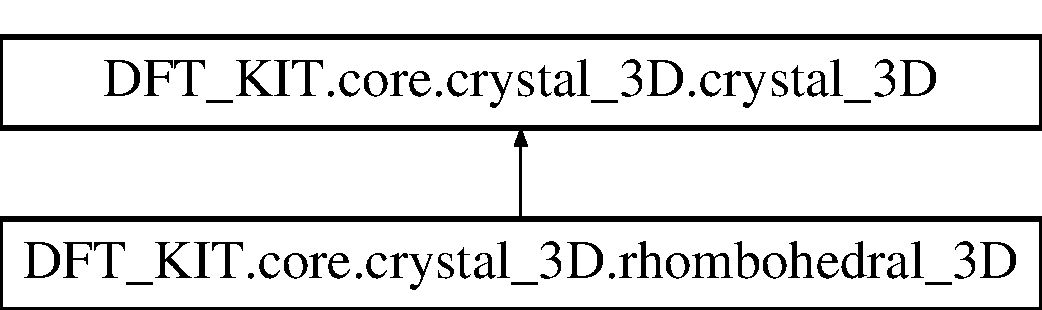
\includegraphics[height=2.000000cm]{class_d_f_t___k_i_t_1_1core_1_1crystal__3_d_1_1rhombohedral__3_d}
\end{center}
\end{figure}
\subsection*{Public Member Functions}
\begin{DoxyCompactItemize}
\item 
def \hyperlink{class_d_f_t___k_i_t_1_1core_1_1crystal__3_d_1_1rhombohedral__3_d_ad04ca9c76614233152251088a1e1c3b7}{\+\_\+\+\_\+init\+\_\+\+\_\+}
\item 
def \hyperlink{class_d_f_t___k_i_t_1_1core_1_1crystal__3_d_1_1rhombohedral__3_d_a35e7f8c7c0508e7038d0ea6e9e17f78d}{set\+\_\+lattice}
\item 
def \hyperlink{class_d_f_t___k_i_t_1_1core_1_1crystal__3_d_1_1rhombohedral__3_d_ac302290201e57719240d3c3be72589ca}{define\+\_\+klabels}
\end{DoxyCompactItemize}
\subsection*{Additional Inherited Members}


\subsection{Detailed Description}


Definition at line 345 of file crystal\+\_\+3\+D.\+py.



\subsection{Constructor \& Destructor Documentation}
\hypertarget{class_d_f_t___k_i_t_1_1core_1_1crystal__3_d_1_1rhombohedral__3_d_ad04ca9c76614233152251088a1e1c3b7}{\index{D\+F\+T\+\_\+\+K\+I\+T\+::core\+::crystal\+\_\+3\+D\+::rhombohedral\+\_\+3\+D@{D\+F\+T\+\_\+\+K\+I\+T\+::core\+::crystal\+\_\+3\+D\+::rhombohedral\+\_\+3\+D}!\+\_\+\+\_\+init\+\_\+\+\_\+@{\+\_\+\+\_\+init\+\_\+\+\_\+}}
\index{\+\_\+\+\_\+init\+\_\+\+\_\+@{\+\_\+\+\_\+init\+\_\+\+\_\+}!D\+F\+T\+\_\+\+K\+I\+T\+::core\+::crystal\+\_\+3\+D\+::rhombohedral\+\_\+3\+D@{D\+F\+T\+\_\+\+K\+I\+T\+::core\+::crystal\+\_\+3\+D\+::rhombohedral\+\_\+3\+D}}
\subsubsection[{\+\_\+\+\_\+init\+\_\+\+\_\+}]{\setlength{\rightskip}{0pt plus 5cm}def D\+F\+T\+\_\+\+K\+I\+T.\+core.\+crystal\+\_\+3\+D.\+rhombohedral\+\_\+3\+D.\+\_\+\+\_\+init\+\_\+\+\_\+ (
\begin{DoxyParamCaption}
\item[{}]{self, }
\item[{}]{rhom\+\_\+length, }
\item[{}]{angle, }
\item[{}]{length\+\_\+unit = {\ttfamily 1.0}}
\end{DoxyParamCaption}
)}}\label{class_d_f_t___k_i_t_1_1core_1_1crystal__3_d_1_1rhombohedral__3_d_ad04ca9c76614233152251088a1e1c3b7}


Definition at line 346 of file crystal\+\_\+3\+D.\+py.



\subsection{Member Function Documentation}
\hypertarget{class_d_f_t___k_i_t_1_1core_1_1crystal__3_d_1_1rhombohedral__3_d_ac302290201e57719240d3c3be72589ca}{\index{D\+F\+T\+\_\+\+K\+I\+T\+::core\+::crystal\+\_\+3\+D\+::rhombohedral\+\_\+3\+D@{D\+F\+T\+\_\+\+K\+I\+T\+::core\+::crystal\+\_\+3\+D\+::rhombohedral\+\_\+3\+D}!define\+\_\+klabels@{define\+\_\+klabels}}
\index{define\+\_\+klabels@{define\+\_\+klabels}!D\+F\+T\+\_\+\+K\+I\+T\+::core\+::crystal\+\_\+3\+D\+::rhombohedral\+\_\+3\+D@{D\+F\+T\+\_\+\+K\+I\+T\+::core\+::crystal\+\_\+3\+D\+::rhombohedral\+\_\+3\+D}}
\subsubsection[{define\+\_\+klabels}]{\setlength{\rightskip}{0pt plus 5cm}def D\+F\+T\+\_\+\+K\+I\+T.\+core.\+crystal\+\_\+3\+D.\+rhombohedral\+\_\+3\+D.\+define\+\_\+klabels (
\begin{DoxyParamCaption}
\item[{}]{self}
\end{DoxyParamCaption}
)}}\label{class_d_f_t___k_i_t_1_1core_1_1crystal__3_d_1_1rhombohedral__3_d_ac302290201e57719240d3c3be72589ca}


Definition at line 367 of file crystal\+\_\+3\+D.\+py.

\hypertarget{class_d_f_t___k_i_t_1_1core_1_1crystal__3_d_1_1rhombohedral__3_d_a35e7f8c7c0508e7038d0ea6e9e17f78d}{\index{D\+F\+T\+\_\+\+K\+I\+T\+::core\+::crystal\+\_\+3\+D\+::rhombohedral\+\_\+3\+D@{D\+F\+T\+\_\+\+K\+I\+T\+::core\+::crystal\+\_\+3\+D\+::rhombohedral\+\_\+3\+D}!set\+\_\+lattice@{set\+\_\+lattice}}
\index{set\+\_\+lattice@{set\+\_\+lattice}!D\+F\+T\+\_\+\+K\+I\+T\+::core\+::crystal\+\_\+3\+D\+::rhombohedral\+\_\+3\+D@{D\+F\+T\+\_\+\+K\+I\+T\+::core\+::crystal\+\_\+3\+D\+::rhombohedral\+\_\+3\+D}}
\subsubsection[{set\+\_\+lattice}]{\setlength{\rightskip}{0pt plus 5cm}def D\+F\+T\+\_\+\+K\+I\+T.\+core.\+crystal\+\_\+3\+D.\+rhombohedral\+\_\+3\+D.\+set\+\_\+lattice (
\begin{DoxyParamCaption}
\item[{}]{self, }
\item[{}]{rhom\+\_\+length, }
\item[{}]{angle\+\_\+}
\end{DoxyParamCaption}
)}}\label{class_d_f_t___k_i_t_1_1core_1_1crystal__3_d_1_1rhombohedral__3_d_a35e7f8c7c0508e7038d0ea6e9e17f78d}


Definition at line 353 of file crystal\+\_\+3\+D.\+py.



The documentation for this class was generated from the following file\+:\begin{DoxyCompactItemize}
\item 
core/\hyperlink{crystal__3_d_8py}{crystal\+\_\+3\+D.\+py}\end{DoxyCompactItemize}

\hypertarget{class_d_f_t___k_i_t_1_1apps_1_1crystal__structure_1_1rocksalt}{\section{D\+F\+T\+\_\+\+K\+I\+T.\+apps.\+crystal\+\_\+structure.\+rocksalt Class Reference}
\label{class_d_f_t___k_i_t_1_1apps_1_1crystal__structure_1_1rocksalt}\index{D\+F\+T\+\_\+\+K\+I\+T.\+apps.\+crystal\+\_\+structure.\+rocksalt@{D\+F\+T\+\_\+\+K\+I\+T.\+apps.\+crystal\+\_\+structure.\+rocksalt}}
}
Inheritance diagram for D\+F\+T\+\_\+\+K\+I\+T.\+apps.\+crystal\+\_\+structure.\+rocksalt\+:\begin{figure}[H]
\begin{center}
\leavevmode
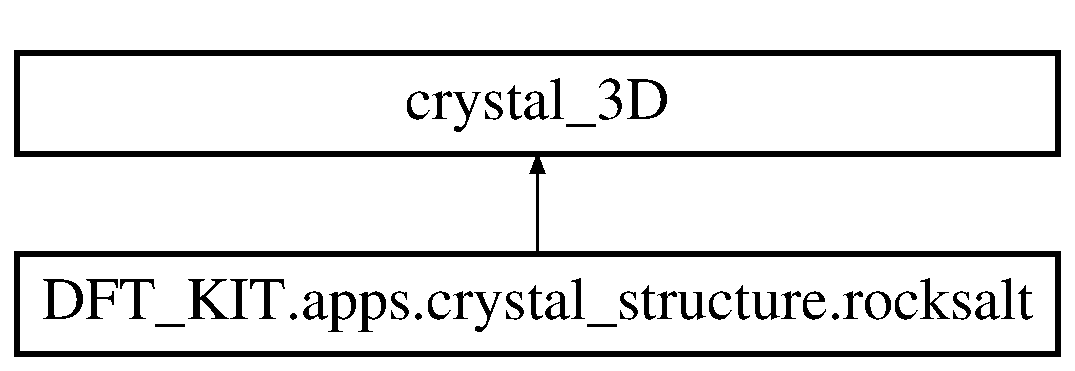
\includegraphics[height=2.000000cm]{class_d_f_t___k_i_t_1_1apps_1_1crystal__structure_1_1rocksalt}
\end{center}
\end{figure}
\subsection*{Public Member Functions}
\begin{DoxyCompactItemize}
\item 
def \hyperlink{class_d_f_t___k_i_t_1_1apps_1_1crystal__structure_1_1rocksalt_aa61780261289f4e7bc5667cf9079770b}{\+\_\+\+\_\+init\+\_\+\+\_\+}
\end{DoxyCompactItemize}


\subsection{Detailed Description}


Definition at line 56 of file crystal\+\_\+structure.\+py.



\subsection{Constructor \& Destructor Documentation}
\hypertarget{class_d_f_t___k_i_t_1_1apps_1_1crystal__structure_1_1rocksalt_aa61780261289f4e7bc5667cf9079770b}{\index{D\+F\+T\+\_\+\+K\+I\+T\+::apps\+::crystal\+\_\+structure\+::rocksalt@{D\+F\+T\+\_\+\+K\+I\+T\+::apps\+::crystal\+\_\+structure\+::rocksalt}!\+\_\+\+\_\+init\+\_\+\+\_\+@{\+\_\+\+\_\+init\+\_\+\+\_\+}}
\index{\+\_\+\+\_\+init\+\_\+\+\_\+@{\+\_\+\+\_\+init\+\_\+\+\_\+}!D\+F\+T\+\_\+\+K\+I\+T\+::apps\+::crystal\+\_\+structure\+::rocksalt@{D\+F\+T\+\_\+\+K\+I\+T\+::apps\+::crystal\+\_\+structure\+::rocksalt}}
\subsubsection[{\+\_\+\+\_\+init\+\_\+\+\_\+}]{\setlength{\rightskip}{0pt plus 5cm}def D\+F\+T\+\_\+\+K\+I\+T.\+apps.\+crystal\+\_\+structure.\+rocksalt.\+\_\+\+\_\+init\+\_\+\+\_\+ (
\begin{DoxyParamCaption}
\item[{}]{self, }
\item[{}]{length\+\_\+unit = {\ttfamily 1.0}}
\end{DoxyParamCaption}
)}}\label{class_d_f_t___k_i_t_1_1apps_1_1crystal__structure_1_1rocksalt_aa61780261289f4e7bc5667cf9079770b}


Definition at line 57 of file crystal\+\_\+structure.\+py.



The documentation for this class was generated from the following file\+:\begin{DoxyCompactItemize}
\item 
apps/\hyperlink{crystal__structure_8py}{crystal\+\_\+structure.\+py}\end{DoxyCompactItemize}

\hypertarget{class_d_f_t___k_i_t_1_1core_1_1general__tool_1_1segments}{\section{D\+F\+T\+\_\+\+K\+I\+T.\+core.\+general\+\_\+tool.\+segments Class Reference}
\label{class_d_f_t___k_i_t_1_1core_1_1general__tool_1_1segments}\index{D\+F\+T\+\_\+\+K\+I\+T.\+core.\+general\+\_\+tool.\+segments@{D\+F\+T\+\_\+\+K\+I\+T.\+core.\+general\+\_\+tool.\+segments}}
}
\subsection*{Public Member Functions}
\begin{DoxyCompactItemize}
\item 
def \hyperlink{class_d_f_t___k_i_t_1_1core_1_1general__tool_1_1segments_adfec2b28f9409ba7b437408fea8bc4d5}{\+\_\+\+\_\+init\+\_\+\+\_\+}
\item 
def \hyperlink{class_d_f_t___k_i_t_1_1core_1_1general__tool_1_1segments_a51ab40998b2deb1f02ac2520df449e53}{get\+\_\+ordering}
\item 
def \hyperlink{class_d_f_t___k_i_t_1_1core_1_1general__tool_1_1segments_a8d26485594d32ed90de52bc4928f821b}{print\+\_\+ordering}
\item 
def \hyperlink{class_d_f_t___k_i_t_1_1core_1_1general__tool_1_1segments_afbcfbca2cf664c5990d0ae83ef06d41d}{swap\+\_\+groups}
\item 
def \hyperlink{class_d_f_t___k_i_t_1_1core_1_1general__tool_1_1segments_a62a39fe2711a1f658e0940dcc8baa57a}{invert\+\_\+group}
\end{DoxyCompactItemize}
\subsection*{Public Attributes}
\begin{DoxyCompactItemize}
\item 
\hyperlink{class_d_f_t___k_i_t_1_1core_1_1general__tool_1_1segments_afa99d60924f0e9d5cf6ffb65086e1738}{ordering}
\item 
\hyperlink{class_d_f_t___k_i_t_1_1core_1_1general__tool_1_1segments_a31cec9678be9764616990406e3056d9a}{subnum}
\item 
\hyperlink{class_d_f_t___k_i_t_1_1core_1_1general__tool_1_1segments_a64d6f15485f3da291d97112c2ba36def}{sets}
\item 
\hyperlink{class_d_f_t___k_i_t_1_1core_1_1general__tool_1_1segments_a70f1faf836f9db631178da335a4f3679}{tmp1}
\item 
\hyperlink{class_d_f_t___k_i_t_1_1core_1_1general__tool_1_1segments_ab34ef602f88d29a1fa594154e1ed9d5d}{tmp2}
\item 
\hyperlink{class_d_f_t___k_i_t_1_1core_1_1general__tool_1_1segments_abb8c06dd79b8e5e9df52c9f30aa6af48}{tmp0}
\end{DoxyCompactItemize}


\subsection{Detailed Description}


Definition at line 8 of file general\+\_\+tool.\+py.



\subsection{Constructor \& Destructor Documentation}
\hypertarget{class_d_f_t___k_i_t_1_1core_1_1general__tool_1_1segments_adfec2b28f9409ba7b437408fea8bc4d5}{\index{D\+F\+T\+\_\+\+K\+I\+T\+::core\+::general\+\_\+tool\+::segments@{D\+F\+T\+\_\+\+K\+I\+T\+::core\+::general\+\_\+tool\+::segments}!\+\_\+\+\_\+init\+\_\+\+\_\+@{\+\_\+\+\_\+init\+\_\+\+\_\+}}
\index{\+\_\+\+\_\+init\+\_\+\+\_\+@{\+\_\+\+\_\+init\+\_\+\+\_\+}!D\+F\+T\+\_\+\+K\+I\+T\+::core\+::general\+\_\+tool\+::segments@{D\+F\+T\+\_\+\+K\+I\+T\+::core\+::general\+\_\+tool\+::segments}}
\subsubsection[{\+\_\+\+\_\+init\+\_\+\+\_\+}]{\setlength{\rightskip}{0pt plus 5cm}def D\+F\+T\+\_\+\+K\+I\+T.\+core.\+general\+\_\+tool.\+segments.\+\_\+\+\_\+init\+\_\+\+\_\+ (
\begin{DoxyParamCaption}
\item[{}]{self, }
\item[{}]{num\+\_\+, }
\item[{}]{sets\+\_\+}
\end{DoxyParamCaption}
)}}\label{class_d_f_t___k_i_t_1_1core_1_1general__tool_1_1segments_adfec2b28f9409ba7b437408fea8bc4d5}


Definition at line 9 of file general\+\_\+tool.\+py.



\subsection{Member Function Documentation}
\hypertarget{class_d_f_t___k_i_t_1_1core_1_1general__tool_1_1segments_a51ab40998b2deb1f02ac2520df449e53}{\index{D\+F\+T\+\_\+\+K\+I\+T\+::core\+::general\+\_\+tool\+::segments@{D\+F\+T\+\_\+\+K\+I\+T\+::core\+::general\+\_\+tool\+::segments}!get\+\_\+ordering@{get\+\_\+ordering}}
\index{get\+\_\+ordering@{get\+\_\+ordering}!D\+F\+T\+\_\+\+K\+I\+T\+::core\+::general\+\_\+tool\+::segments@{D\+F\+T\+\_\+\+K\+I\+T\+::core\+::general\+\_\+tool\+::segments}}
\subsubsection[{get\+\_\+ordering}]{\setlength{\rightskip}{0pt plus 5cm}def D\+F\+T\+\_\+\+K\+I\+T.\+core.\+general\+\_\+tool.\+segments.\+get\+\_\+ordering (
\begin{DoxyParamCaption}
\item[{}]{self}
\end{DoxyParamCaption}
)}}\label{class_d_f_t___k_i_t_1_1core_1_1general__tool_1_1segments_a51ab40998b2deb1f02ac2520df449e53}


Definition at line 16 of file general\+\_\+tool.\+py.

\hypertarget{class_d_f_t___k_i_t_1_1core_1_1general__tool_1_1segments_a62a39fe2711a1f658e0940dcc8baa57a}{\index{D\+F\+T\+\_\+\+K\+I\+T\+::core\+::general\+\_\+tool\+::segments@{D\+F\+T\+\_\+\+K\+I\+T\+::core\+::general\+\_\+tool\+::segments}!invert\+\_\+group@{invert\+\_\+group}}
\index{invert\+\_\+group@{invert\+\_\+group}!D\+F\+T\+\_\+\+K\+I\+T\+::core\+::general\+\_\+tool\+::segments@{D\+F\+T\+\_\+\+K\+I\+T\+::core\+::general\+\_\+tool\+::segments}}
\subsubsection[{invert\+\_\+group}]{\setlength{\rightskip}{0pt plus 5cm}def D\+F\+T\+\_\+\+K\+I\+T.\+core.\+general\+\_\+tool.\+segments.\+invert\+\_\+group (
\begin{DoxyParamCaption}
\item[{}]{self, }
\item[{}]{group\+\_\+}
\end{DoxyParamCaption}
)}}\label{class_d_f_t___k_i_t_1_1core_1_1general__tool_1_1segments_a62a39fe2711a1f658e0940dcc8baa57a}


Definition at line 25 of file general\+\_\+tool.\+py.

\hypertarget{class_d_f_t___k_i_t_1_1core_1_1general__tool_1_1segments_a8d26485594d32ed90de52bc4928f821b}{\index{D\+F\+T\+\_\+\+K\+I\+T\+::core\+::general\+\_\+tool\+::segments@{D\+F\+T\+\_\+\+K\+I\+T\+::core\+::general\+\_\+tool\+::segments}!print\+\_\+ordering@{print\+\_\+ordering}}
\index{print\+\_\+ordering@{print\+\_\+ordering}!D\+F\+T\+\_\+\+K\+I\+T\+::core\+::general\+\_\+tool\+::segments@{D\+F\+T\+\_\+\+K\+I\+T\+::core\+::general\+\_\+tool\+::segments}}
\subsubsection[{print\+\_\+ordering}]{\setlength{\rightskip}{0pt plus 5cm}def D\+F\+T\+\_\+\+K\+I\+T.\+core.\+general\+\_\+tool.\+segments.\+print\+\_\+ordering (
\begin{DoxyParamCaption}
\item[{}]{self}
\end{DoxyParamCaption}
)}}\label{class_d_f_t___k_i_t_1_1core_1_1general__tool_1_1segments_a8d26485594d32ed90de52bc4928f821b}


Definition at line 18 of file general\+\_\+tool.\+py.

\hypertarget{class_d_f_t___k_i_t_1_1core_1_1general__tool_1_1segments_afbcfbca2cf664c5990d0ae83ef06d41d}{\index{D\+F\+T\+\_\+\+K\+I\+T\+::core\+::general\+\_\+tool\+::segments@{D\+F\+T\+\_\+\+K\+I\+T\+::core\+::general\+\_\+tool\+::segments}!swap\+\_\+groups@{swap\+\_\+groups}}
\index{swap\+\_\+groups@{swap\+\_\+groups}!D\+F\+T\+\_\+\+K\+I\+T\+::core\+::general\+\_\+tool\+::segments@{D\+F\+T\+\_\+\+K\+I\+T\+::core\+::general\+\_\+tool\+::segments}}
\subsubsection[{swap\+\_\+groups}]{\setlength{\rightskip}{0pt plus 5cm}def D\+F\+T\+\_\+\+K\+I\+T.\+core.\+general\+\_\+tool.\+segments.\+swap\+\_\+groups (
\begin{DoxyParamCaption}
\item[{}]{self, }
\item[{}]{group1, }
\item[{}]{group2}
\end{DoxyParamCaption}
)}}\label{class_d_f_t___k_i_t_1_1core_1_1general__tool_1_1segments_afbcfbca2cf664c5990d0ae83ef06d41d}


Definition at line 20 of file general\+\_\+tool.\+py.



\subsection{Member Data Documentation}
\hypertarget{class_d_f_t___k_i_t_1_1core_1_1general__tool_1_1segments_afa99d60924f0e9d5cf6ffb65086e1738}{\index{D\+F\+T\+\_\+\+K\+I\+T\+::core\+::general\+\_\+tool\+::segments@{D\+F\+T\+\_\+\+K\+I\+T\+::core\+::general\+\_\+tool\+::segments}!ordering@{ordering}}
\index{ordering@{ordering}!D\+F\+T\+\_\+\+K\+I\+T\+::core\+::general\+\_\+tool\+::segments@{D\+F\+T\+\_\+\+K\+I\+T\+::core\+::general\+\_\+tool\+::segments}}
\subsubsection[{ordering}]{\setlength{\rightskip}{0pt plus 5cm}D\+F\+T\+\_\+\+K\+I\+T.\+core.\+general\+\_\+tool.\+segments.\+ordering}}\label{class_d_f_t___k_i_t_1_1core_1_1general__tool_1_1segments_afa99d60924f0e9d5cf6ffb65086e1738}


Definition at line 10 of file general\+\_\+tool.\+py.

\hypertarget{class_d_f_t___k_i_t_1_1core_1_1general__tool_1_1segments_a64d6f15485f3da291d97112c2ba36def}{\index{D\+F\+T\+\_\+\+K\+I\+T\+::core\+::general\+\_\+tool\+::segments@{D\+F\+T\+\_\+\+K\+I\+T\+::core\+::general\+\_\+tool\+::segments}!sets@{sets}}
\index{sets@{sets}!D\+F\+T\+\_\+\+K\+I\+T\+::core\+::general\+\_\+tool\+::segments@{D\+F\+T\+\_\+\+K\+I\+T\+::core\+::general\+\_\+tool\+::segments}}
\subsubsection[{sets}]{\setlength{\rightskip}{0pt plus 5cm}D\+F\+T\+\_\+\+K\+I\+T.\+core.\+general\+\_\+tool.\+segments.\+sets}}\label{class_d_f_t___k_i_t_1_1core_1_1general__tool_1_1segments_a64d6f15485f3da291d97112c2ba36def}


Definition at line 12 of file general\+\_\+tool.\+py.

\hypertarget{class_d_f_t___k_i_t_1_1core_1_1general__tool_1_1segments_a31cec9678be9764616990406e3056d9a}{\index{D\+F\+T\+\_\+\+K\+I\+T\+::core\+::general\+\_\+tool\+::segments@{D\+F\+T\+\_\+\+K\+I\+T\+::core\+::general\+\_\+tool\+::segments}!subnum@{subnum}}
\index{subnum@{subnum}!D\+F\+T\+\_\+\+K\+I\+T\+::core\+::general\+\_\+tool\+::segments@{D\+F\+T\+\_\+\+K\+I\+T\+::core\+::general\+\_\+tool\+::segments}}
\subsubsection[{subnum}]{\setlength{\rightskip}{0pt plus 5cm}D\+F\+T\+\_\+\+K\+I\+T.\+core.\+general\+\_\+tool.\+segments.\+subnum}}\label{class_d_f_t___k_i_t_1_1core_1_1general__tool_1_1segments_a31cec9678be9764616990406e3056d9a}


Definition at line 11 of file general\+\_\+tool.\+py.

\hypertarget{class_d_f_t___k_i_t_1_1core_1_1general__tool_1_1segments_abb8c06dd79b8e5e9df52c9f30aa6af48}{\index{D\+F\+T\+\_\+\+K\+I\+T\+::core\+::general\+\_\+tool\+::segments@{D\+F\+T\+\_\+\+K\+I\+T\+::core\+::general\+\_\+tool\+::segments}!tmp0@{tmp0}}
\index{tmp0@{tmp0}!D\+F\+T\+\_\+\+K\+I\+T\+::core\+::general\+\_\+tool\+::segments@{D\+F\+T\+\_\+\+K\+I\+T\+::core\+::general\+\_\+tool\+::segments}}
\subsubsection[{tmp0}]{\setlength{\rightskip}{0pt plus 5cm}D\+F\+T\+\_\+\+K\+I\+T.\+core.\+general\+\_\+tool.\+segments.\+tmp0}}\label{class_d_f_t___k_i_t_1_1core_1_1general__tool_1_1segments_abb8c06dd79b8e5e9df52c9f30aa6af48}


Definition at line 15 of file general\+\_\+tool.\+py.

\hypertarget{class_d_f_t___k_i_t_1_1core_1_1general__tool_1_1segments_a70f1faf836f9db631178da335a4f3679}{\index{D\+F\+T\+\_\+\+K\+I\+T\+::core\+::general\+\_\+tool\+::segments@{D\+F\+T\+\_\+\+K\+I\+T\+::core\+::general\+\_\+tool\+::segments}!tmp1@{tmp1}}
\index{tmp1@{tmp1}!D\+F\+T\+\_\+\+K\+I\+T\+::core\+::general\+\_\+tool\+::segments@{D\+F\+T\+\_\+\+K\+I\+T\+::core\+::general\+\_\+tool\+::segments}}
\subsubsection[{tmp1}]{\setlength{\rightskip}{0pt plus 5cm}D\+F\+T\+\_\+\+K\+I\+T.\+core.\+general\+\_\+tool.\+segments.\+tmp1}}\label{class_d_f_t___k_i_t_1_1core_1_1general__tool_1_1segments_a70f1faf836f9db631178da335a4f3679}


Definition at line 13 of file general\+\_\+tool.\+py.

\hypertarget{class_d_f_t___k_i_t_1_1core_1_1general__tool_1_1segments_ab34ef602f88d29a1fa594154e1ed9d5d}{\index{D\+F\+T\+\_\+\+K\+I\+T\+::core\+::general\+\_\+tool\+::segments@{D\+F\+T\+\_\+\+K\+I\+T\+::core\+::general\+\_\+tool\+::segments}!tmp2@{tmp2}}
\index{tmp2@{tmp2}!D\+F\+T\+\_\+\+K\+I\+T\+::core\+::general\+\_\+tool\+::segments@{D\+F\+T\+\_\+\+K\+I\+T\+::core\+::general\+\_\+tool\+::segments}}
\subsubsection[{tmp2}]{\setlength{\rightskip}{0pt plus 5cm}D\+F\+T\+\_\+\+K\+I\+T.\+core.\+general\+\_\+tool.\+segments.\+tmp2}}\label{class_d_f_t___k_i_t_1_1core_1_1general__tool_1_1segments_ab34ef602f88d29a1fa594154e1ed9d5d}


Definition at line 14 of file general\+\_\+tool.\+py.



The documentation for this class was generated from the following file\+:\begin{DoxyCompactItemize}
\item 
core/\hyperlink{general__tool_8py}{general\+\_\+tool.\+py}\end{DoxyCompactItemize}

\hypertarget{class_d_f_t___k_i_t_1_1core_1_1crystal__3_d_1_1tetragonal__3_d}{\section{D\+F\+T\+\_\+\+K\+I\+T.\+core.\+crystal\+\_\+3\+D.\+tetragonal\+\_\+3\+D Class Reference}
\label{class_d_f_t___k_i_t_1_1core_1_1crystal__3_d_1_1tetragonal__3_d}\index{D\+F\+T\+\_\+\+K\+I\+T.\+core.\+crystal\+\_\+3\+D.\+tetragonal\+\_\+3\+D@{D\+F\+T\+\_\+\+K\+I\+T.\+core.\+crystal\+\_\+3\+D.\+tetragonal\+\_\+3\+D}}
}
Inheritance diagram for D\+F\+T\+\_\+\+K\+I\+T.\+core.\+crystal\+\_\+3\+D.\+tetragonal\+\_\+3\+D\+:\begin{figure}[H]
\begin{center}
\leavevmode
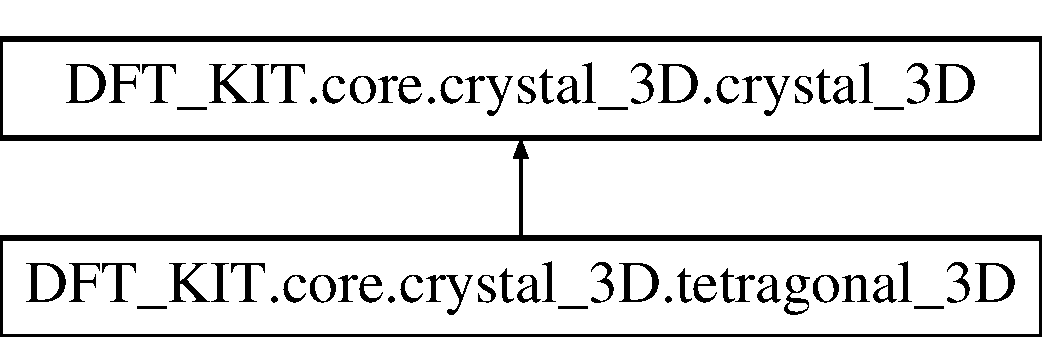
\includegraphics[height=2.000000cm]{class_d_f_t___k_i_t_1_1core_1_1crystal__3_d_1_1tetragonal__3_d}
\end{center}
\end{figure}
\subsection*{Public Member Functions}
\begin{DoxyCompactItemize}
\item 
def \hyperlink{class_d_f_t___k_i_t_1_1core_1_1crystal__3_d_1_1tetragonal__3_d_a24ae7396b4310496b17aa319e8a2a45e}{\+\_\+\+\_\+init\+\_\+\+\_\+}
\item 
def \hyperlink{class_d_f_t___k_i_t_1_1core_1_1crystal__3_d_1_1tetragonal__3_d_a9302cfb0437f54df09c9cccae87ee513}{set\+\_\+lattice}
\item 
def \hyperlink{class_d_f_t___k_i_t_1_1core_1_1crystal__3_d_1_1tetragonal__3_d_a64368867ccdec5433773434d01a87c97}{define\+\_\+klabels}
\end{DoxyCompactItemize}
\subsection*{Additional Inherited Members}


\subsection{Detailed Description}


Definition at line 252 of file crystal\+\_\+3\+D.\+py.



\subsection{Constructor \& Destructor Documentation}
\hypertarget{class_d_f_t___k_i_t_1_1core_1_1crystal__3_d_1_1tetragonal__3_d_a24ae7396b4310496b17aa319e8a2a45e}{\index{D\+F\+T\+\_\+\+K\+I\+T\+::core\+::crystal\+\_\+3\+D\+::tetragonal\+\_\+3\+D@{D\+F\+T\+\_\+\+K\+I\+T\+::core\+::crystal\+\_\+3\+D\+::tetragonal\+\_\+3\+D}!\+\_\+\+\_\+init\+\_\+\+\_\+@{\+\_\+\+\_\+init\+\_\+\+\_\+}}
\index{\+\_\+\+\_\+init\+\_\+\+\_\+@{\+\_\+\+\_\+init\+\_\+\+\_\+}!D\+F\+T\+\_\+\+K\+I\+T\+::core\+::crystal\+\_\+3\+D\+::tetragonal\+\_\+3\+D@{D\+F\+T\+\_\+\+K\+I\+T\+::core\+::crystal\+\_\+3\+D\+::tetragonal\+\_\+3\+D}}
\subsubsection[{\+\_\+\+\_\+init\+\_\+\+\_\+}]{\setlength{\rightskip}{0pt plus 5cm}def D\+F\+T\+\_\+\+K\+I\+T.\+core.\+crystal\+\_\+3\+D.\+tetragonal\+\_\+3\+D.\+\_\+\+\_\+init\+\_\+\+\_\+ (
\begin{DoxyParamCaption}
\item[{}]{self, }
\item[{}]{a\+\_\+ = {\ttfamily 0.0}, }
\item[{}]{c\+\_\+ = {\ttfamily 0.0}, }
\item[{}]{length\+\_\+unit = {\ttfamily 1.0}}
\end{DoxyParamCaption}
)}}\label{class_d_f_t___k_i_t_1_1core_1_1crystal__3_d_1_1tetragonal__3_d_a24ae7396b4310496b17aa319e8a2a45e}


Definition at line 253 of file crystal\+\_\+3\+D.\+py.



\subsection{Member Function Documentation}
\hypertarget{class_d_f_t___k_i_t_1_1core_1_1crystal__3_d_1_1tetragonal__3_d_a64368867ccdec5433773434d01a87c97}{\index{D\+F\+T\+\_\+\+K\+I\+T\+::core\+::crystal\+\_\+3\+D\+::tetragonal\+\_\+3\+D@{D\+F\+T\+\_\+\+K\+I\+T\+::core\+::crystal\+\_\+3\+D\+::tetragonal\+\_\+3\+D}!define\+\_\+klabels@{define\+\_\+klabels}}
\index{define\+\_\+klabels@{define\+\_\+klabels}!D\+F\+T\+\_\+\+K\+I\+T\+::core\+::crystal\+\_\+3\+D\+::tetragonal\+\_\+3\+D@{D\+F\+T\+\_\+\+K\+I\+T\+::core\+::crystal\+\_\+3\+D\+::tetragonal\+\_\+3\+D}}
\subsubsection[{define\+\_\+klabels}]{\setlength{\rightskip}{0pt plus 5cm}def D\+F\+T\+\_\+\+K\+I\+T.\+core.\+crystal\+\_\+3\+D.\+tetragonal\+\_\+3\+D.\+define\+\_\+klabels (
\begin{DoxyParamCaption}
\item[{}]{self}
\end{DoxyParamCaption}
)}}\label{class_d_f_t___k_i_t_1_1core_1_1crystal__3_d_1_1tetragonal__3_d_a64368867ccdec5433773434d01a87c97}


Definition at line 264 of file crystal\+\_\+3\+D.\+py.

\hypertarget{class_d_f_t___k_i_t_1_1core_1_1crystal__3_d_1_1tetragonal__3_d_a9302cfb0437f54df09c9cccae87ee513}{\index{D\+F\+T\+\_\+\+K\+I\+T\+::core\+::crystal\+\_\+3\+D\+::tetragonal\+\_\+3\+D@{D\+F\+T\+\_\+\+K\+I\+T\+::core\+::crystal\+\_\+3\+D\+::tetragonal\+\_\+3\+D}!set\+\_\+lattice@{set\+\_\+lattice}}
\index{set\+\_\+lattice@{set\+\_\+lattice}!D\+F\+T\+\_\+\+K\+I\+T\+::core\+::crystal\+\_\+3\+D\+::tetragonal\+\_\+3\+D@{D\+F\+T\+\_\+\+K\+I\+T\+::core\+::crystal\+\_\+3\+D\+::tetragonal\+\_\+3\+D}}
\subsubsection[{set\+\_\+lattice}]{\setlength{\rightskip}{0pt plus 5cm}def D\+F\+T\+\_\+\+K\+I\+T.\+core.\+crystal\+\_\+3\+D.\+tetragonal\+\_\+3\+D.\+set\+\_\+lattice (
\begin{DoxyParamCaption}
\item[{}]{self, }
\item[{}]{a\+\_\+, }
\item[{}]{c\+\_\+}
\end{DoxyParamCaption}
)}}\label{class_d_f_t___k_i_t_1_1core_1_1crystal__3_d_1_1tetragonal__3_d_a9302cfb0437f54df09c9cccae87ee513}


Definition at line 258 of file crystal\+\_\+3\+D.\+py.



The documentation for this class was generated from the following file\+:\begin{DoxyCompactItemize}
\item 
core/\hyperlink{crystal__3_d_8py}{crystal\+\_\+3\+D.\+py}\end{DoxyCompactItemize}

\hypertarget{class_d_f_t___k_i_t_1_1core_1_1crystal__3_d_1_1triclinic__3_d}{\section{D\+F\+T\+\_\+\+K\+I\+T.\+core.\+crystal\+\_\+3\+D.\+triclinic\+\_\+3\+D Class Reference}
\label{class_d_f_t___k_i_t_1_1core_1_1crystal__3_d_1_1triclinic__3_d}\index{D\+F\+T\+\_\+\+K\+I\+T.\+core.\+crystal\+\_\+3\+D.\+triclinic\+\_\+3\+D@{D\+F\+T\+\_\+\+K\+I\+T.\+core.\+crystal\+\_\+3\+D.\+triclinic\+\_\+3\+D}}
}
Inheritance diagram for D\+F\+T\+\_\+\+K\+I\+T.\+core.\+crystal\+\_\+3\+D.\+triclinic\+\_\+3\+D\+:\begin{figure}[H]
\begin{center}
\leavevmode
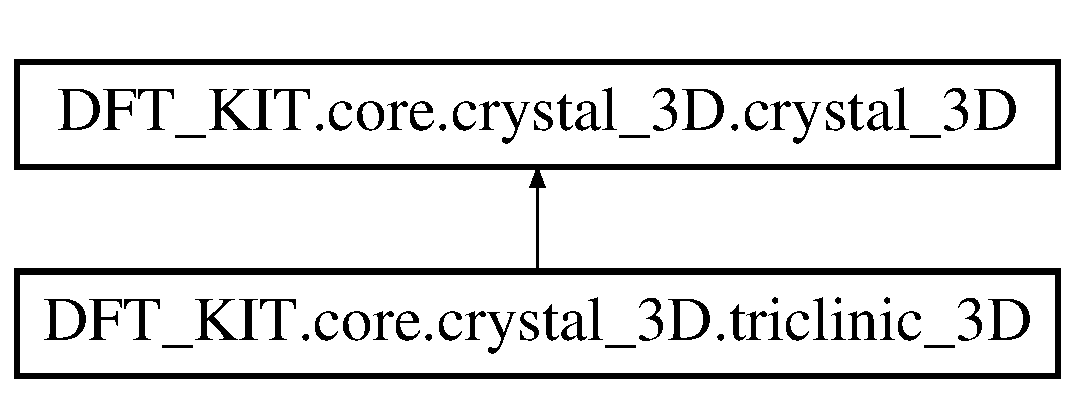
\includegraphics[height=2.000000cm]{class_d_f_t___k_i_t_1_1core_1_1crystal__3_d_1_1triclinic__3_d}
\end{center}
\end{figure}
\subsection*{Public Member Functions}
\begin{DoxyCompactItemize}
\item 
def \hyperlink{class_d_f_t___k_i_t_1_1core_1_1crystal__3_d_1_1triclinic__3_d_adc82f93ad5bd06a39519d84d2d7dc653}{\+\_\+\+\_\+init\+\_\+\+\_\+}
\item 
def \hyperlink{class_d_f_t___k_i_t_1_1core_1_1crystal__3_d_1_1triclinic__3_d_a6bc4b124df096336888c92ea43ec1158}{set\+\_\+lattice\+\_\+constant}
\end{DoxyCompactItemize}
\subsection*{Additional Inherited Members}


\subsection{Detailed Description}


Definition at line 331 of file crystal\+\_\+3\+D.\+py.



\subsection{Constructor \& Destructor Documentation}
\hypertarget{class_d_f_t___k_i_t_1_1core_1_1crystal__3_d_1_1triclinic__3_d_adc82f93ad5bd06a39519d84d2d7dc653}{\index{D\+F\+T\+\_\+\+K\+I\+T\+::core\+::crystal\+\_\+3\+D\+::triclinic\+\_\+3\+D@{D\+F\+T\+\_\+\+K\+I\+T\+::core\+::crystal\+\_\+3\+D\+::triclinic\+\_\+3\+D}!\+\_\+\+\_\+init\+\_\+\+\_\+@{\+\_\+\+\_\+init\+\_\+\+\_\+}}
\index{\+\_\+\+\_\+init\+\_\+\+\_\+@{\+\_\+\+\_\+init\+\_\+\+\_\+}!D\+F\+T\+\_\+\+K\+I\+T\+::core\+::crystal\+\_\+3\+D\+::triclinic\+\_\+3\+D@{D\+F\+T\+\_\+\+K\+I\+T\+::core\+::crystal\+\_\+3\+D\+::triclinic\+\_\+3\+D}}
\subsubsection[{\+\_\+\+\_\+init\+\_\+\+\_\+}]{\setlength{\rightskip}{0pt plus 5cm}def D\+F\+T\+\_\+\+K\+I\+T.\+core.\+crystal\+\_\+3\+D.\+triclinic\+\_\+3\+D.\+\_\+\+\_\+init\+\_\+\+\_\+ (
\begin{DoxyParamCaption}
\item[{}]{self, }
\item[{}]{a\+\_\+ = {\ttfamily 0.0}, }
\item[{}]{b\+\_\+ = {\ttfamily 0.0}, }
\item[{}]{c\+\_\+ = {\ttfamily 0.0}, }
\item[{}]{angle\+\_\+ = {\ttfamily 0.0}, }
\item[{}]{length\+\_\+unit = {\ttfamily 1.0}}
\end{DoxyParamCaption}
)}}\label{class_d_f_t___k_i_t_1_1core_1_1crystal__3_d_1_1triclinic__3_d_adc82f93ad5bd06a39519d84d2d7dc653}


Definition at line 333 of file crystal\+\_\+3\+D.\+py.



\subsection{Member Function Documentation}
\hypertarget{class_d_f_t___k_i_t_1_1core_1_1crystal__3_d_1_1triclinic__3_d_a6bc4b124df096336888c92ea43ec1158}{\index{D\+F\+T\+\_\+\+K\+I\+T\+::core\+::crystal\+\_\+3\+D\+::triclinic\+\_\+3\+D@{D\+F\+T\+\_\+\+K\+I\+T\+::core\+::crystal\+\_\+3\+D\+::triclinic\+\_\+3\+D}!set\+\_\+lattice\+\_\+constant@{set\+\_\+lattice\+\_\+constant}}
\index{set\+\_\+lattice\+\_\+constant@{set\+\_\+lattice\+\_\+constant}!D\+F\+T\+\_\+\+K\+I\+T\+::core\+::crystal\+\_\+3\+D\+::triclinic\+\_\+3\+D@{D\+F\+T\+\_\+\+K\+I\+T\+::core\+::crystal\+\_\+3\+D\+::triclinic\+\_\+3\+D}}
\subsubsection[{set\+\_\+lattice\+\_\+constant}]{\setlength{\rightskip}{0pt plus 5cm}def D\+F\+T\+\_\+\+K\+I\+T.\+core.\+crystal\+\_\+3\+D.\+triclinic\+\_\+3\+D.\+set\+\_\+lattice\+\_\+constant (
\begin{DoxyParamCaption}
\item[{}]{self, }
\item[{}]{a\+\_\+, }
\item[{}]{b\+\_\+, }
\item[{}]{c\+\_\+, }
\item[{}]{angle\+\_\+}
\end{DoxyParamCaption}
)}}\label{class_d_f_t___k_i_t_1_1core_1_1crystal__3_d_1_1triclinic__3_d_a6bc4b124df096336888c92ea43ec1158}


Definition at line 337 of file crystal\+\_\+3\+D.\+py.



The documentation for this class was generated from the following file\+:\begin{DoxyCompactItemize}
\item 
core/\hyperlink{crystal__3_d_8py}{crystal\+\_\+3\+D.\+py}\end{DoxyCompactItemize}

\chapter{File Documentation}
\hypertarget{____init_____8py}{\section{\+\_\+\+\_\+init\+\_\+\+\_\+.\+py File Reference}
\label{____init_____8py}\index{\+\_\+\+\_\+init\+\_\+\+\_\+.\+py@{\+\_\+\+\_\+init\+\_\+\+\_\+.\+py}}
}
\subsection*{Namespaces}
\begin{DoxyCompactItemize}
\item 
 \hyperlink{namespace_d_f_t___k_i_t}{D\+F\+T\+\_\+\+K\+I\+T}
\end{DoxyCompactItemize}

\hypertarget{apps_2____init_____8py}{\section{apps/\+\_\+\+\_\+init\+\_\+\+\_\+.py File Reference}
\label{apps_2____init_____8py}\index{apps/\+\_\+\+\_\+init\+\_\+\+\_\+.\+py@{apps/\+\_\+\+\_\+init\+\_\+\+\_\+.\+py}}
}
\subsection*{Namespaces}
\begin{DoxyCompactItemize}
\item 
 \hyperlink{namespace_d_f_t___k_i_t_1_1apps}{D\+F\+T\+\_\+\+K\+I\+T.\+apps}
\end{DoxyCompactItemize}

\hypertarget{calculator_2____init_____8py}{\section{calculator/\+\_\+\+\_\+init\+\_\+\+\_\+.py File Reference}
\label{calculator_2____init_____8py}\index{calculator/\+\_\+\+\_\+init\+\_\+\+\_\+.\+py@{calculator/\+\_\+\+\_\+init\+\_\+\+\_\+.\+py}}
}
\subsection*{Namespaces}
\begin{DoxyCompactItemize}
\item 
 \hyperlink{namespace_d_f_t___k_i_t_1_1calculator}{D\+F\+T\+\_\+\+K\+I\+T.\+calculator}
\end{DoxyCompactItemize}

\hypertarget{core_2____init_____8py}{\section{core/\+\_\+\+\_\+init\+\_\+\+\_\+.py File Reference}
\label{core_2____init_____8py}\index{core/\+\_\+\+\_\+init\+\_\+\+\_\+.\+py@{core/\+\_\+\+\_\+init\+\_\+\+\_\+.\+py}}
}
\subsection*{Namespaces}
\begin{DoxyCompactItemize}
\item 
 \hyperlink{namespace_d_f_t___k_i_t_1_1core}{D\+F\+T\+\_\+\+K\+I\+T.\+core}
\end{DoxyCompactItemize}

\hypertarget{interface_2____init_____8py}{\section{interface/\+\_\+\+\_\+init\+\_\+\+\_\+.py File Reference}
\label{interface_2____init_____8py}\index{interface/\+\_\+\+\_\+init\+\_\+\+\_\+.\+py@{interface/\+\_\+\+\_\+init\+\_\+\+\_\+.\+py}}
}
\subsection*{Namespaces}
\begin{DoxyCompactItemize}
\item 
 \hyperlink{namespace_d_f_t___k_i_t_1_1interface}{D\+F\+T\+\_\+\+K\+I\+T.\+interface}
\end{DoxyCompactItemize}

\hypertarget{bismuth__antimony_8py}{\section{apps/bismuth\+\_\+antimony.py File Reference}
\label{bismuth__antimony_8py}\index{apps/bismuth\+\_\+antimony.\+py@{apps/bismuth\+\_\+antimony.\+py}}
}
\subsection*{Namespaces}
\begin{DoxyCompactItemize}
\item 
 \hyperlink{namespace_d_f_t___k_i_t_1_1apps_1_1bismuth__antimony}{D\+F\+T\+\_\+\+K\+I\+T.\+apps.\+bismuth\+\_\+antimony}
\end{DoxyCompactItemize}
\subsection*{Variables}
\begin{DoxyCompactItemize}
\item 
dictionary \hyperlink{namespace_d_f_t___k_i_t_1_1apps_1_1bismuth__antimony_aa1abaca0360ca74cc7aff767b2f8b339}{D\+F\+T\+\_\+\+K\+I\+T.\+apps.\+bismuth\+\_\+antimony.\+Sb\+\_\+exp\+\_\+1} = \{'lattice\+\_\+constant'\+:4.\+489,'angle'\+:(57.\+0+14.\+0/60.\+0)$\ast$np.\+pi/180.\+0,'rhom\+\_\+u'\+:0.\+2336\}
\item 
dictionary \hyperlink{namespace_d_f_t___k_i_t_1_1apps_1_1bismuth__antimony_a241f6ef77b95d1682e324b5c0e2ef2e9}{D\+F\+T\+\_\+\+K\+I\+T.\+apps.\+bismuth\+\_\+antimony.\+Sb\+\_\+exp\+\_\+2} = \{'lattice\+\_\+constant'\+:4.\+4898,'angle'\+:(57.\+233)$\ast$np.\+pi/180.\+0,'rhom\+\_\+u'\+:0.\+23362\}
\item 
tuple \hyperlink{namespace_d_f_t___k_i_t_1_1apps_1_1bismuth__antimony_a93eb1699becde1ccbaea30f9f2a83c48}{D\+F\+T\+\_\+\+K\+I\+T.\+apps.\+bismuth\+\_\+antimony.\+Sb} = element.\+element('Sb',121.\+760,51,5,vasp\+\_\+pot='Sb',qes\+\_\+pot='')
\item 
tuple \hyperlink{namespace_d_f_t___k_i_t_1_1apps_1_1bismuth__antimony_a98b6587f573c187c59bed3eb7ba473ec}{D\+F\+T\+\_\+\+K\+I\+T.\+apps.\+bismuth\+\_\+antimony.\+Sb\+\_\+d} = element.\+element('Sb',121.\+760,51,15,vasp\+\_\+pot='Sb\+\_\+d',qes\+\_\+pot='')
\item 
dictionary \hyperlink{namespace_d_f_t___k_i_t_1_1apps_1_1bismuth__antimony_ac29eda409a16938d88021a96729db286}{D\+F\+T\+\_\+\+K\+I\+T.\+apps.\+bismuth\+\_\+antimony.\+Sb\+\_\+vasp\+\_\+scf} = \{\}
\item 
dictionary \hyperlink{namespace_d_f_t___k_i_t_1_1apps_1_1bismuth__antimony_aaf0784cd6faa22be296849a9edac5b29}{D\+F\+T\+\_\+\+K\+I\+T.\+apps.\+bismuth\+\_\+antimony.\+Sb\+\_\+vasp\+\_\+nscf\+\_\+soi} = \{\}
\item 
dictionary \hyperlink{namespace_d_f_t___k_i_t_1_1apps_1_1bismuth__antimony_a0e0f7c4aa8d0742ba96eaa32092c4d38}{D\+F\+T\+\_\+\+K\+I\+T.\+apps.\+bismuth\+\_\+antimony.\+Sb\+\_\+qespresso\+\_\+scf} = \{\}
\item 
dictionary \hyperlink{namespace_d_f_t___k_i_t_1_1apps_1_1bismuth__antimony_a59fa5c238b4d21bbc0313b00f42bbfe9}{D\+F\+T\+\_\+\+K\+I\+T.\+apps.\+bismuth\+\_\+antimony.\+Sb\+\_\+qespresso\+\_\+nscf\+\_\+soi} = \{\}
\item 
dictionary \hyperlink{namespace_d_f_t___k_i_t_1_1apps_1_1bismuth__antimony_a0ea685695e01c80f5dce15e6982ed14d}{D\+F\+T\+\_\+\+K\+I\+T.\+apps.\+bismuth\+\_\+antimony.\+Sb\+\_\+wannier90} = \{\}
\item 
dictionary \hyperlink{namespace_d_f_t___k_i_t_1_1apps_1_1bismuth__antimony_a3897eb47b9a6eba72bc4280a6b6d41fd}{D\+F\+T\+\_\+\+K\+I\+T.\+apps.\+bismuth\+\_\+antimony.\+Bi\+\_\+exp\+\_\+1} = \{'lattice\+\_\+constant'\+:4.\+7212,'angle'\+:(57.\+0+19.\+0/60.\+0)$\ast$np.\+pi/180.\+0,'rhom\+\_\+u'\+:0.\+23407\}
\item 
dictionary \hyperlink{namespace_d_f_t___k_i_t_1_1apps_1_1bismuth__antimony_a2fc8afe0ae0f1828d58e0a064cd3a844}{D\+F\+T\+\_\+\+K\+I\+T.\+apps.\+bismuth\+\_\+antimony.\+Bi\+\_\+exp\+\_\+2} = \{'lattice\+\_\+constant'\+:4.\+7236,'angle'\+:(57.\+35)$\ast$np.\+pi/180.\+0,'rhom\+\_\+u'\+:0.\+23407\}
\item 
dictionary \hyperlink{namespace_d_f_t___k_i_t_1_1apps_1_1bismuth__antimony_ad3ff489e1051aa82103c3da7dc7b6b5f}{D\+F\+T\+\_\+\+K\+I\+T.\+apps.\+bismuth\+\_\+antimony.\+Bi\+\_\+dft\+\_\+1} = \{'lattice\+\_\+constant'\+:4.\+7973,'angle'\+:(53.\+0+56.\+0/60.\+0)$\ast$np.\+pi/180.\+0,'rhom\+\_\+u'\+:0.\+2348\}
\item 
dictionary \hyperlink{namespace_d_f_t___k_i_t_1_1apps_1_1bismuth__antimony_af07069b59f7b4092160fafe6e87f7dc1}{D\+F\+T\+\_\+\+K\+I\+T.\+apps.\+bismuth\+\_\+antimony.\+Bi\+\_\+dft\+\_\+2} = \{'lattice\+\_\+constant'\+:4.\+7827,'angle'\+:(56.\+0+17.\+0/60.\+0)$\ast$np.\+pi/180.\+0,'rhom\+\_\+u'\+:0.\+2351\}
\item 
dictionary \hyperlink{namespace_d_f_t___k_i_t_1_1apps_1_1bismuth__antimony_a985fb7de2187991f21de822473d66fc5}{D\+F\+T\+\_\+\+K\+I\+T.\+apps.\+bismuth\+\_\+antimony.\+Bi\+\_\+dft\+\_\+3} = \{'lattice\+\_\+constant'\+:4.\+8038,'angle'\+:(53.\+0+36.\+0/60.\+0)$\ast$np.\+pi/180.\+0,'rhom\+\_\+u'\+:0.\+2347\}
\item 
tuple \hyperlink{namespace_d_f_t___k_i_t_1_1apps_1_1bismuth__antimony_a47d28bdcd6f82edb8765d6a4ca9654f7}{D\+F\+T\+\_\+\+K\+I\+T.\+apps.\+bismuth\+\_\+antimony.\+Bi\+\_\+exp} = element.\+element('Bi',208.\+9804,83,5,vasp\+\_\+pot='Bi',qes\+\_\+pot='Bi.\+U\+P\+F',rhom\+\_\+length=4.\+7236,angle=1.\+0009,rhom\+\_\+u=0.\+23407)
\item 
tuple \hyperlink{namespace_d_f_t___k_i_t_1_1apps_1_1bismuth__antimony_a09c7ba05ea616d81e4ba1eeec01e4fc0}{D\+F\+T\+\_\+\+K\+I\+T.\+apps.\+bismuth\+\_\+antimony.\+Bi\+\_\+d} = element.\+element('Bi',208.\+9804,83,15,vasp\+\_\+pot='Bi\+\_\+d',qes\+\_\+pot='')
\item 
dictionary \hyperlink{namespace_d_f_t___k_i_t_1_1apps_1_1bismuth__antimony_af1379b9e75a375b0b047a28c450c122c}{D\+F\+T\+\_\+\+K\+I\+T.\+apps.\+bismuth\+\_\+antimony.\+Bi\+\_\+vasp\+\_\+slab\+\_\+scf} = \{\}
\item 
dictionary \hyperlink{namespace_d_f_t___k_i_t_1_1apps_1_1bismuth__antimony_a564e9fe84c344988895e95377f1361a3}{D\+F\+T\+\_\+\+K\+I\+T.\+apps.\+bismuth\+\_\+antimony.\+Bi\+\_\+vasp\+\_\+slab\+\_\+nscf\+\_\+soi} = \{\}
\item 
dictionary \hyperlink{namespace_d_f_t___k_i_t_1_1apps_1_1bismuth__antimony_ab475abbbc15cd01fa76531119b87d038}{D\+F\+T\+\_\+\+K\+I\+T.\+apps.\+bismuth\+\_\+antimony.\+Bi\+\_\+vasp\+\_\+crystal\+\_\+scf} = \{'I\+S\+T\+A\+R\+T'\+:'0','E\+N\+C\+U\+T'\+:'250','E\+D\+I\+F\+F'\+:'1\+E-\/6','\+I\+S\+M\+E\+A\+R'\+:'-\/5','\+S\+I\+G\+M\+A'\+:'0.\+2','\+L\+M\+A\+X\+M\+I\+X'\+:'4'\}
\item 
dictionary \hyperlink{namespace_d_f_t___k_i_t_1_1apps_1_1bismuth__antimony_a44bfb7c33246a8a0aba68758b5fa94fa}{D\+F\+T\+\_\+\+K\+I\+T.\+apps.\+bismuth\+\_\+antimony.\+Bi\+\_\+vasp\+\_\+crystal\+\_\+nscf\+\_\+soi} = \{'I\+S\+T\+A\+R\+T'\+:'0','I\+C\+H\+A\+R\+G'\+:'11','E\+N\+C\+U\+T'\+:'250','E\+D\+I\+F\+F'\+:'1\+E-\/6','\+G\+G\+A\+\_\+\+C\+O\+M\+P\+A\+T'\+:'.\+F\+A\+L\+S\+E.','\+I\+S\+Y\+M'\+:'0','\+S\+A\+X\+I\+S'\+:'0 0 1','\+L\+S\+O\+R\+B\+I\+T'\+:'.\+T\+R\+U\+E.','\+L\+M\+A\+X\+M\+I\+X'\+:'4','\+M\+A\+G\+M\+O\+M'\+:\+True\}
\item 
dictionary \hyperlink{namespace_d_f_t___k_i_t_1_1apps_1_1bismuth__antimony_acca8f4e3d0ae5de1c3bd1aee18a91917}{D\+F\+T\+\_\+\+K\+I\+T.\+apps.\+bismuth\+\_\+antimony.\+Bi\+\_\+qespresso\+\_\+crystal\+\_\+scf} = \{\}
\item 
dictionary \hyperlink{namespace_d_f_t___k_i_t_1_1apps_1_1bismuth__antimony_a2d9ad25d1a2a764b263a0f0c9cfef67d}{D\+F\+T\+\_\+\+K\+I\+T.\+apps.\+bismuth\+\_\+antimony.\+Bi\+\_\+qespresso\+\_\+crystal\+\_\+nscf\+\_\+soi} = \{\}
\item 
dictionary \hyperlink{namespace_d_f_t___k_i_t_1_1apps_1_1bismuth__antimony_a3a42f256e90e6cba1809e1b6caa9f168}{D\+F\+T\+\_\+\+K\+I\+T.\+apps.\+bismuth\+\_\+antimony.\+Bi\+\_\+qespresso\+\_\+slab\+\_\+scf} = \{\}
\item 
dictionary \hyperlink{namespace_d_f_t___k_i_t_1_1apps_1_1bismuth__antimony_a364bff2bee5cb80746d82205c445ad7c}{D\+F\+T\+\_\+\+K\+I\+T.\+apps.\+bismuth\+\_\+antimony.\+Bi\+\_\+qespresso\+\_\+slab\+\_\+nscf\+\_\+soi} = \{\}
\item 
dictionary \hyperlink{namespace_d_f_t___k_i_t_1_1apps_1_1bismuth__antimony_a95707d9864da25fbccf902580ebaecd0}{D\+F\+T\+\_\+\+K\+I\+T.\+apps.\+bismuth\+\_\+antimony.\+Bi\+\_\+wannier90} = \{\}
\end{DoxyCompactItemize}

\hypertarget{crystal__structure_8py}{\section{apps/crystal\+\_\+structure.py File Reference}
\label{crystal__structure_8py}\index{apps/crystal\+\_\+structure.\+py@{apps/crystal\+\_\+structure.\+py}}
}
\subsection*{Classes}
\begin{DoxyCompactItemize}
\item 
class \hyperlink{class_d_f_t___k_i_t_1_1apps_1_1crystal__structure_1_1a7__structure}{D\+F\+T\+\_\+\+K\+I\+T.\+apps.\+crystal\+\_\+structure.\+a7\+\_\+structure}
\item 
class \hyperlink{class_d_f_t___k_i_t_1_1apps_1_1crystal__structure_1_1graphene}{D\+F\+T\+\_\+\+K\+I\+T.\+apps.\+crystal\+\_\+structure.\+graphene}
\item 
class \hyperlink{class_d_f_t___k_i_t_1_1apps_1_1crystal__structure_1_1layer__material}{D\+F\+T\+\_\+\+K\+I\+T.\+apps.\+crystal\+\_\+structure.\+layer\+\_\+material}
\item 
class \hyperlink{class_d_f_t___k_i_t_1_1apps_1_1crystal__structure_1_1diamond}{D\+F\+T\+\_\+\+K\+I\+T.\+apps.\+crystal\+\_\+structure.\+diamond}
\item 
class \hyperlink{class_d_f_t___k_i_t_1_1apps_1_1crystal__structure_1_1perovskite}{D\+F\+T\+\_\+\+K\+I\+T.\+apps.\+crystal\+\_\+structure.\+perovskite}
\item 
class \hyperlink{class_d_f_t___k_i_t_1_1apps_1_1crystal__structure_1_1rocksalt}{D\+F\+T\+\_\+\+K\+I\+T.\+apps.\+crystal\+\_\+structure.\+rocksalt}
\item 
class \hyperlink{class_d_f_t___k_i_t_1_1apps_1_1crystal__structure_1_1body__center}{D\+F\+T\+\_\+\+K\+I\+T.\+apps.\+crystal\+\_\+structure.\+body\+\_\+center}
\item 
class \hyperlink{class_d_f_t___k_i_t_1_1apps_1_1crystal__structure_1_1face__center}{D\+F\+T\+\_\+\+K\+I\+T.\+apps.\+crystal\+\_\+structure.\+face\+\_\+center}
\end{DoxyCompactItemize}
\subsection*{Namespaces}
\begin{DoxyCompactItemize}
\item 
 \hyperlink{namespace_d_f_t___k_i_t_1_1apps_1_1crystal__structure}{D\+F\+T\+\_\+\+K\+I\+T.\+apps.\+crystal\+\_\+structure}
\end{DoxyCompactItemize}

\hypertarget{dft__cmdtool_8py}{\section{apps/dft\+\_\+cmdtool.py File Reference}
\label{dft__cmdtool_8py}\index{apps/dft\+\_\+cmdtool.\+py@{apps/dft\+\_\+cmdtool.\+py}}
}
\subsection*{Namespaces}
\begin{DoxyCompactItemize}
\item 
 \hyperlink{namespace_d_f_t___k_i_t_1_1apps_1_1dft__cmdtool}{D\+F\+T\+\_\+\+K\+I\+T.\+apps.\+dft\+\_\+cmdtool}
\end{DoxyCompactItemize}
\subsection*{Variables}
\begin{DoxyCompactItemize}
\item 
tuple \hyperlink{namespace_d_f_t___k_i_t_1_1apps_1_1dft__cmdtool_a199f85e4cd240a8ea565d8d8638cca2e}{D\+F\+T\+\_\+\+K\+I\+T.\+apps.\+dft\+\_\+cmdtool.\+dft\+\_\+job} = job.\+job(False)
\item 
tuple \hyperlink{namespace_d_f_t___k_i_t_1_1apps_1_1dft__cmdtool_ae64fc152ecc9625928d1b894c9509b63}{D\+F\+T\+\_\+\+K\+I\+T.\+apps.\+dft\+\_\+cmdtool.\+root\+\_\+dir} = os.\+getcwd()
\item 
tuple \hyperlink{namespace_d_f_t___k_i_t_1_1apps_1_1dft__cmdtool_ad379ce6f66c010b507abcc8decec82c6}{D\+F\+T\+\_\+\+K\+I\+T.\+apps.\+dft\+\_\+cmdtool.\+numargs} = len(sys.\+argv)
\item 
list \hyperlink{namespace_d_f_t___k_i_t_1_1apps_1_1dft__cmdtool_ad9689f4893a4dde9249d301ef1d932e0}{D\+F\+T\+\_\+\+K\+I\+T.\+apps.\+dft\+\_\+cmdtool.\+scriptfile} = sys.\+argv\mbox{[}1\mbox{]}
\item 
tuple \hyperlink{namespace_d_f_t___k_i_t_1_1apps_1_1dft__cmdtool_aa0e3413d9ae4c07c0b02d807cdc6db8f}{D\+F\+T\+\_\+\+K\+I\+T.\+apps.\+dft\+\_\+cmdtool.\+input\+\_\+cmd} = dft\+\_\+job.\+get\+\_\+info('dft\+\_\+cmdtool','input command',True)
\item 
tuple \hyperlink{namespace_d_f_t___k_i_t_1_1apps_1_1dft__cmdtool_a2f9c5ee4d542f8399dd8338856ee309c}{D\+F\+T\+\_\+\+K\+I\+T.\+apps.\+dft\+\_\+cmdtool.\+cmd\+\_\+first} = input\+\_\+cmd.\+split()
\item 
tuple \hyperlink{namespace_d_f_t___k_i_t_1_1apps_1_1dft__cmdtool_a4df77ff242ff65823d46090c1f2264a9}{D\+F\+T\+\_\+\+K\+I\+T.\+apps.\+dft\+\_\+cmdtool.\+cmd\+\_\+num} = len(input\+\_\+cmd.\+split())
\item 
tuple \hyperlink{namespace_d_f_t___k_i_t_1_1apps_1_1dft__cmdtool_ae4e59628a7aea11f8ee1b4f913d7f6e3}{D\+F\+T\+\_\+\+K\+I\+T.\+apps.\+dft\+\_\+cmdtool.\+cmds} = input\+\_\+cmd.\+split()
\end{DoxyCompactItemize}

\hypertarget{slab__surface__rhom_8py}{\section{apps/slab\+\_\+surface\+\_\+rhom.py File Reference}
\label{slab__surface__rhom_8py}\index{apps/slab\+\_\+surface\+\_\+rhom.\+py@{apps/slab\+\_\+surface\+\_\+rhom.\+py}}
}
\subsection*{Classes}
\begin{DoxyCompactItemize}
\item 
class \hyperlink{class_d_f_t___k_i_t_1_1apps_1_1slab__surface__rhom_1_1_rhom__trigonal__surface}{D\+F\+T\+\_\+\+K\+I\+T.\+apps.\+slab\+\_\+surface\+\_\+rhom.\+Rhom\+\_\+trigonal\+\_\+surface}
\item 
class \hyperlink{class_d_f_t___k_i_t_1_1apps_1_1slab__surface__rhom_1_1_rhom__parallel__trigonal__surface}{D\+F\+T\+\_\+\+K\+I\+T.\+apps.\+slab\+\_\+surface\+\_\+rhom.\+Rhom\+\_\+parallel\+\_\+trigonal\+\_\+surface}
\end{DoxyCompactItemize}
\subsection*{Namespaces}
\begin{DoxyCompactItemize}
\item 
 \hyperlink{namespace_d_f_t___k_i_t_1_1apps_1_1slab__surface__rhom}{D\+F\+T\+\_\+\+K\+I\+T.\+apps.\+slab\+\_\+surface\+\_\+rhom}
\end{DoxyCompactItemize}

\hypertarget{wire__rhom_8py}{\section{apps/wire\+\_\+rhom.py File Reference}
\label{wire__rhom_8py}\index{apps/wire\+\_\+rhom.\+py@{apps/wire\+\_\+rhom.\+py}}
}
\subsection*{Classes}
\begin{DoxyCompactItemize}
\item 
class \hyperlink{class_d_f_t___k_i_t_1_1apps_1_1wire__rhom_1_1_rhom__trigonal__nanowire}{D\+F\+T\+\_\+\+K\+I\+T.\+apps.\+wire\+\_\+rhom.\+Rhom\+\_\+trigonal\+\_\+nanowire}
\end{DoxyCompactItemize}
\subsection*{Namespaces}
\begin{DoxyCompactItemize}
\item 
 \hyperlink{namespace_d_f_t___k_i_t_1_1apps_1_1wire__rhom}{D\+F\+T\+\_\+\+K\+I\+T.\+apps.\+wire\+\_\+rhom}
\end{DoxyCompactItemize}

\hypertarget{_q_e_s_p_r_e_s_s_o_8py}{\section{calculator/\+Q\+E\+S\+P\+R\+E\+S\+S\+O.py File Reference}
\label{_q_e_s_p_r_e_s_s_o_8py}\index{calculator/\+Q\+E\+S\+P\+R\+E\+S\+S\+O.\+py@{calculator/\+Q\+E\+S\+P\+R\+E\+S\+S\+O.\+py}}
}
\subsection*{Classes}
\begin{DoxyCompactItemize}
\item 
class \hyperlink{class_d_f_t___k_i_t_1_1calculator_1_1_q_e_s_p_r_e_s_s_o_1_1calculator___q_e_s_p_r_e_s_s_o}{D\+F\+T\+\_\+\+K\+I\+T.\+calculator.\+Q\+E\+S\+P\+R\+E\+S\+S\+O.\+calculator\+\_\+\+Q\+E\+S\+P\+R\+E\+S\+S\+O}
\end{DoxyCompactItemize}
\subsection*{Namespaces}
\begin{DoxyCompactItemize}
\item 
 \hyperlink{namespace_d_f_t___k_i_t_1_1calculator_1_1_q_e_s_p_r_e_s_s_o}{D\+F\+T\+\_\+\+K\+I\+T.\+calculator.\+Q\+E\+S\+P\+R\+E\+S\+S\+O}
\end{DoxyCompactItemize}
\subsection*{Variables}
\begin{DoxyCompactItemize}
\item 
string \hyperlink{namespace_d_f_t___k_i_t_1_1calculator_1_1_q_e_s_p_r_e_s_s_o_af7b03c15432c08ac6f347a3a09d50a3f}{D\+F\+T\+\_\+\+K\+I\+T.\+calculator.\+Q\+E\+S\+P\+R\+E\+S\+S\+O.\+Q\+E\+S\+\_\+control\+\_\+flags} = 'calculation title verbosity restart\+\_\+mode wf\+\_\+collect nstep iprint tstress tprnfor dt wfcdir lkpoint\+\_\+dir max\+\_\+seconds etot\+\_\+conv\+\_\+thr forc\+\_\+conv\+\_\+thr disk\+\_\+io tefield dipfield lelfield nberrycyc lorbm lberry gdir nppstr'
\item 
string \hyperlink{namespace_d_f_t___k_i_t_1_1calculator_1_1_q_e_s_p_r_e_s_s_o_a4fc2949def8bc4b8a2802d0e542f63dc}{D\+F\+T\+\_\+\+K\+I\+T.\+calculator.\+Q\+E\+S\+P\+R\+E\+S\+S\+O.\+Q\+E\+S\+\_\+system\+\_\+flags} = 'ibrav celldm A B C cos\+A\+B cos\+A\+C cos\+B\+C nbnd tot\+\_\+charge tot\+\_\+magnetization starting\+\_\+magnetization ecutwfc ecutrho ecutfock nr1 nr2 nr3 nr1s nr2s nr3s nosym nosym\+\_\+evc noinv no\+\_\+t\+\_\+rev force\+\_\+symmorphic use\+\_\+all\+\_\+frac occupations one\+\_\+atom\+\_\+occupations starting\+\_\+spin\+\_\+angle degauss smearing nspin noncolin ecfixed qcutz q2sigma input\+\_\+dft exx\+\_\+fraction screening\+\_\+parameter exxdiv\+\_\+treatment x\+\_\+gamma\+\_\+extrapolation ecutvcut nqx1 nqx2 nqx3 lda\+\_\+plus\+\_\+u lda\+\_\+plus\+\_\+u\+\_\+kind Hubbard\+\_\+\+U Hubbard\+\_\+\+J0 Hubbard\+\_\+alpha Hubbard\+\_\+beta Hubbard\+\_\+\+J(i,ityp) starting\+\_\+ns\+\_\+eigenvalue(m,ispin,I) U\+\_\+projection\+\_\+type edir emaxpos eopreg eamp angle1 angle2 constrained\+\_\+magnetization fixed\+\_\+magnetization lambda report lspinorb assume\+\_\+isolated esm\+\_\+bc esm\+\_\+w esm\+\_\+efield esm\+\_\+nfit vdw\+\_\+corr london london\+\_\+s6 london\+\_\+rcut xdm xdm\+\_\+a1 xdm\+\_\+a2'
\item 
string \hyperlink{namespace_d_f_t___k_i_t_1_1calculator_1_1_q_e_s_p_r_e_s_s_o_a36e40202edc11d7e727685fe0f5661f0}{D\+F\+T\+\_\+\+K\+I\+T.\+calculator.\+Q\+E\+S\+P\+R\+E\+S\+S\+O.\+Q\+E\+S\+\_\+electrons\+\_\+flags} = 'electron\+\_\+maxstep scf\+\_\+must\+\_\+converge conv\+\_\+thr adaptive\+\_\+thr conv\+\_\+thr\+\_\+init conv\+\_\+thr\+\_\+multi mixing\+\_\+mode mixing\+\_\+beta mixing\+\_\+ndim mixing\+\_\+fixed\+\_\+ns diagonalization ortho\+\_\+para diago\+\_\+thr\+\_\+init diago\+\_\+cg\+\_\+maxiter diago\+\_\+david\+\_\+ndim diago\+\_\+full\+\_\+acc efield efield\+\_\+cart startingpot startingwfc tqr'
\item 
string \hyperlink{namespace_d_f_t___k_i_t_1_1calculator_1_1_q_e_s_p_r_e_s_s_o_af16e80a77f76ffc37d94100867ed5eab}{D\+F\+T\+\_\+\+K\+I\+T.\+calculator.\+Q\+E\+S\+P\+R\+E\+S\+S\+O.\+Q\+E\+S\+\_\+ions\+\_\+flags} = 'ion\+\_\+dynamics ion\+\_\+positions phase\+\_\+space pot\+\_\+extrapolation wfc\+\_\+extrapolation remove\+\_\+rigid\+\_\+rot ion\+\_\+temperature tempw tolp delta\+\_\+t nraise refold\+\_\+pos upscale bfgs\+\_\+ndim trust\+\_\+radius\+\_\+max trust\+\_\+radius\+\_\+min trust\+\_\+radius\+\_\+ini w\+\_\+1 w\+\_\+2'
\item 
string \hyperlink{namespace_d_f_t___k_i_t_1_1calculator_1_1_q_e_s_p_r_e_s_s_o_a4f68d41dc1daf471640d1ca11f7770b3}{D\+F\+T\+\_\+\+K\+I\+T.\+calculator.\+Q\+E\+S\+P\+R\+E\+S\+S\+O.\+Q\+E\+S\+\_\+cell\+\_\+flags} = 'cell\+\_\+dynamics press wmass cell\+\_\+factor press\+\_\+conv\+\_\+thr cell\+\_\+dofree'
\item 
list \hyperlink{namespace_d_f_t___k_i_t_1_1calculator_1_1_q_e_s_p_r_e_s_s_o_a652e35119d6363d2d2d36e2da261cf71}{D\+F\+T\+\_\+\+K\+I\+T.\+calculator.\+Q\+E\+S\+P\+R\+E\+S\+S\+O.\+Q\+E\+S\+\_\+\+P\+W2\+W\+A\+N\+\_\+flags} = \mbox{[}'write\+\_\+amn','write\+\_\+spn','write\+\_\+mmn','write\+\_\+unk'\mbox{]}
\end{DoxyCompactItemize}

\hypertarget{script_8py}{\section{calculator/script.py File Reference}
\label{script_8py}\index{calculator/script.\+py@{calculator/script.\+py}}
}
\subsection*{Classes}
\begin{DoxyCompactItemize}
\item 
class \hyperlink{class_d_f_t___k_i_t_1_1calculator_1_1script_1_1calculator__script}{D\+F\+T\+\_\+\+K\+I\+T.\+calculator.\+script.\+calculator\+\_\+script}
\end{DoxyCompactItemize}
\subsection*{Namespaces}
\begin{DoxyCompactItemize}
\item 
 \hyperlink{namespace_d_f_t___k_i_t_1_1calculator_1_1script}{D\+F\+T\+\_\+\+K\+I\+T.\+calculator.\+script}
\end{DoxyCompactItemize}
\subsection*{Variables}
\begin{DoxyCompactItemize}
\item 
list \hyperlink{namespace_d_f_t___k_i_t_1_1calculator_1_1script_a18c2d8c5a8a3cdb3d885e693093e3827}{D\+F\+T\+\_\+\+K\+I\+T.\+calculator.\+script.\+V\+A\+S\+P\+\_\+incar\+\_\+flags}
\item 
list \hyperlink{namespace_d_f_t___k_i_t_1_1calculator_1_1script_ade8f664e5d6258f0719cf5848ccad9b8}{D\+F\+T\+\_\+\+K\+I\+T.\+calculator.\+script.\+V\+A\+S\+P\+\_\+kpoints\+\_\+flags} = \mbox{[}$\,$\mbox{]}
\end{DoxyCompactItemize}

\hypertarget{_s_i_e_s_t_a_8py}{\section{calculator/\+S\+I\+E\+S\+T\+A.py File Reference}
\label{_s_i_e_s_t_a_8py}\index{calculator/\+S\+I\+E\+S\+T\+A.\+py@{calculator/\+S\+I\+E\+S\+T\+A.\+py}}
}
\subsection*{Classes}
\begin{DoxyCompactItemize}
\item 
class \hyperlink{class_d_f_t___k_i_t_1_1calculator_1_1_s_i_e_s_t_a_1_1calculator___s_i_e_s_t_a}{D\+F\+T\+\_\+\+K\+I\+T.\+calculator.\+S\+I\+E\+S\+T\+A.\+calculator\+\_\+\+S\+I\+E\+S\+T\+A}
\end{DoxyCompactItemize}
\subsection*{Namespaces}
\begin{DoxyCompactItemize}
\item 
 \hyperlink{namespace_d_f_t___k_i_t_1_1calculator_1_1_s_i_e_s_t_a}{D\+F\+T\+\_\+\+K\+I\+T.\+calculator.\+S\+I\+E\+S\+T\+A}
\end{DoxyCompactItemize}
\subsection*{Variables}
\begin{DoxyCompactItemize}
\item 
list \hyperlink{namespace_d_f_t___k_i_t_1_1calculator_1_1_s_i_e_s_t_a_ae83e5ef1b4c41f4272ed134b22f6f3c9}{D\+F\+T\+\_\+\+K\+I\+T.\+calculator.\+S\+I\+E\+S\+T\+A.\+S\+I\+E\+S\+T\+A\+\_\+flags}
\item 
string \hyperlink{namespace_d_f_t___k_i_t_1_1calculator_1_1_s_i_e_s_t_a_af058c84c65fdd8bc16fb661c1d552152}{D\+F\+T\+\_\+\+K\+I\+T.\+calculator.\+S\+I\+E\+S\+T\+A.\+S\+I\+E\+\_\+flags}
\end{DoxyCompactItemize}

\hypertarget{_v_a_s_p_8py}{\section{calculator/\+V\+A\+S\+P.py File Reference}
\label{_v_a_s_p_8py}\index{calculator/\+V\+A\+S\+P.\+py@{calculator/\+V\+A\+S\+P.\+py}}
}
\subsection*{Classes}
\begin{DoxyCompactItemize}
\item 
class \hyperlink{class_d_f_t___k_i_t_1_1calculator_1_1_v_a_s_p_1_1calculator___v_a_s_p}{D\+F\+T\+\_\+\+K\+I\+T.\+calculator.\+V\+A\+S\+P.\+calculator\+\_\+\+V\+A\+S\+P}
\end{DoxyCompactItemize}
\subsection*{Namespaces}
\begin{DoxyCompactItemize}
\item 
 \hyperlink{namespace_d_f_t___k_i_t_1_1calculator_1_1_v_a_s_p}{D\+F\+T\+\_\+\+K\+I\+T.\+calculator.\+V\+A\+S\+P}
\end{DoxyCompactItemize}
\subsection*{Variables}
\begin{DoxyCompactItemize}
\item 
list \hyperlink{namespace_d_f_t___k_i_t_1_1calculator_1_1_v_a_s_p_a7690ba9ed849d4f42c86ab05be97222d}{D\+F\+T\+\_\+\+K\+I\+T.\+calculator.\+V\+A\+S\+P.\+V\+A\+S\+P\+\_\+incar\+\_\+flags}
\item 
list \hyperlink{namespace_d_f_t___k_i_t_1_1calculator_1_1_v_a_s_p_a5f56b24ad81644827a028dd152578ba0}{D\+F\+T\+\_\+\+K\+I\+T.\+calculator.\+V\+A\+S\+P.\+V\+A\+S\+P\+\_\+kpoints\+\_\+flags} = \mbox{[}$\,$\mbox{]}
\end{DoxyCompactItemize}

\hypertarget{_wannier90_8py}{\section{calculator/\+Wannier90.py File Reference}
\label{_wannier90_8py}\index{calculator/\+Wannier90.\+py@{calculator/\+Wannier90.\+py}}
}
\subsection*{Classes}
\begin{DoxyCompactItemize}
\item 
class \hyperlink{class_d_f_t___k_i_t_1_1calculator_1_1_wannier90_1_1calculator___wannier90}{D\+F\+T\+\_\+\+K\+I\+T.\+calculator.\+Wannier90.\+calculator\+\_\+\+Wannier90}
\end{DoxyCompactItemize}
\subsection*{Namespaces}
\begin{DoxyCompactItemize}
\item 
 \hyperlink{namespace_d_f_t___k_i_t_1_1calculator_1_1_wannier90}{D\+F\+T\+\_\+\+K\+I\+T.\+calculator.\+Wannier90}
\end{DoxyCompactItemize}
\subsection*{Variables}
\begin{DoxyCompactItemize}
\item 
list \hyperlink{namespace_d_f_t___k_i_t_1_1calculator_1_1_wannier90_ad9950007869589842f2abe7f2c75b877}{D\+F\+T\+\_\+\+K\+I\+T.\+calculator.\+Wannier90.\+Q\+E\+S\+\_\+wannier90\+\_\+flags}
\end{DoxyCompactItemize}

\hypertarget{atom_8py}{\section{core/atom.py File Reference}
\label{atom_8py}\index{core/atom.\+py@{core/atom.\+py}}
}
\subsection*{Classes}
\begin{DoxyCompactItemize}
\item 
class \hyperlink{class_d_f_t___k_i_t_1_1core_1_1atom_1_1atom}{D\+F\+T\+\_\+\+K\+I\+T.\+core.\+atom.\+atom}
\end{DoxyCompactItemize}
\subsection*{Namespaces}
\begin{DoxyCompactItemize}
\item 
 \hyperlink{namespace_d_f_t___k_i_t_1_1core_1_1atom}{D\+F\+T\+\_\+\+K\+I\+T.\+core.\+atom}
\end{DoxyCompactItemize}

\hypertarget{calculator_8py}{\section{core/calculator.py File Reference}
\label{calculator_8py}\index{core/calculator.\+py@{core/calculator.\+py}}
}
\subsection*{Classes}
\begin{DoxyCompactItemize}
\item 
class \hyperlink{class_d_f_t___k_i_t_1_1core_1_1calculator_1_1calculator}{D\+F\+T\+\_\+\+K\+I\+T.\+core.\+calculator.\+calculator}
\end{DoxyCompactItemize}
\subsection*{Namespaces}
\begin{DoxyCompactItemize}
\item 
 \hyperlink{namespace_d_f_t___k_i_t_1_1core_1_1calculator}{D\+F\+T\+\_\+\+K\+I\+T.\+core.\+calculator}
\end{DoxyCompactItemize}

\hypertarget{crystal__3_d_8py}{\section{core/crystal\+\_\+3\+D.py File Reference}
\label{crystal__3_d_8py}\index{core/crystal\+\_\+3\+D.\+py@{core/crystal\+\_\+3\+D.\+py}}
}
\subsection*{Classes}
\begin{DoxyCompactItemize}
\item 
class \hyperlink{class_d_f_t___k_i_t_1_1core_1_1crystal__3_d_1_1crystal__3_d}{D\+F\+T\+\_\+\+K\+I\+T.\+core.\+crystal\+\_\+3\+D.\+crystal\+\_\+3\+D}
\begin{DoxyCompactList}\small\item\em Class for \hyperlink{class_d_f_t___k_i_t_1_1core_1_1crystal__3_d_1_1crystal__3_d}{crystal\+\_\+3\+D}. \end{DoxyCompactList}\item 
class \hyperlink{class_d_f_t___k_i_t_1_1core_1_1crystal__3_d_1_1cubic__3_d}{D\+F\+T\+\_\+\+K\+I\+T.\+core.\+crystal\+\_\+3\+D.\+cubic\+\_\+3\+D}
\item 
class \hyperlink{class_d_f_t___k_i_t_1_1core_1_1crystal__3_d_1_1bcc__3_d}{D\+F\+T\+\_\+\+K\+I\+T.\+core.\+crystal\+\_\+3\+D.\+bcc\+\_\+3\+D}
\item 
class \hyperlink{class_d_f_t___k_i_t_1_1core_1_1crystal__3_d_1_1fcc__3_d}{D\+F\+T\+\_\+\+K\+I\+T.\+core.\+crystal\+\_\+3\+D.\+fcc\+\_\+3\+D}
\item 
class \hyperlink{class_d_f_t___k_i_t_1_1core_1_1crystal__3_d_1_1hexagonal__3_d}{D\+F\+T\+\_\+\+K\+I\+T.\+core.\+crystal\+\_\+3\+D.\+hexagonal\+\_\+3\+D}
\item 
class \hyperlink{class_d_f_t___k_i_t_1_1core_1_1crystal__3_d_1_1tetragonal__3_d}{D\+F\+T\+\_\+\+K\+I\+T.\+core.\+crystal\+\_\+3\+D.\+tetragonal\+\_\+3\+D}
\item 
class \hyperlink{class_d_f_t___k_i_t_1_1core_1_1crystal__3_d_1_1orthorhombic__3_d}{D\+F\+T\+\_\+\+K\+I\+T.\+core.\+crystal\+\_\+3\+D.\+orthorhombic\+\_\+3\+D}
\item 
class \hyperlink{class_d_f_t___k_i_t_1_1core_1_1crystal__3_d_1_1monoclinic__3_d}{D\+F\+T\+\_\+\+K\+I\+T.\+core.\+crystal\+\_\+3\+D.\+monoclinic\+\_\+3\+D}
\item 
class \hyperlink{class_d_f_t___k_i_t_1_1core_1_1crystal__3_d_1_1triclinic__3_d}{D\+F\+T\+\_\+\+K\+I\+T.\+core.\+crystal\+\_\+3\+D.\+triclinic\+\_\+3\+D}
\item 
class \hyperlink{class_d_f_t___k_i_t_1_1core_1_1crystal__3_d_1_1rhombohedral__3_d}{D\+F\+T\+\_\+\+K\+I\+T.\+core.\+crystal\+\_\+3\+D.\+rhombohedral\+\_\+3\+D}
\end{DoxyCompactItemize}
\subsection*{Namespaces}
\begin{DoxyCompactItemize}
\item 
 \hyperlink{namespace_d_f_t___k_i_t_1_1core_1_1crystal__3_d}{D\+F\+T\+\_\+\+K\+I\+T.\+core.\+crystal\+\_\+3\+D}
\end{DoxyCompactItemize}

\hypertarget{element_8py}{\section{core/element.py File Reference}
\label{element_8py}\index{core/element.\+py@{core/element.\+py}}
}
\subsection*{Classes}
\begin{DoxyCompactItemize}
\item 
class \hyperlink{class_d_f_t___k_i_t_1_1core_1_1element_1_1element}{D\+F\+T\+\_\+\+K\+I\+T.\+core.\+element.\+element}
\end{DoxyCompactItemize}
\subsection*{Namespaces}
\begin{DoxyCompactItemize}
\item 
 \hyperlink{namespace_d_f_t___k_i_t_1_1core_1_1element}{D\+F\+T\+\_\+\+K\+I\+T.\+core.\+element}
\end{DoxyCompactItemize}
\subsection*{Functions}
\begin{DoxyCompactItemize}
\item 
def \hyperlink{namespace_d_f_t___k_i_t_1_1core_1_1element_a688120b4538e366222f5299c61e924e4}{D\+F\+T\+\_\+\+K\+I\+T.\+core.\+element.\+chem\+\_\+number}
\item 
def \hyperlink{namespace_d_f_t___k_i_t_1_1core_1_1element_accc4487239f4ac6a7ac203e34e94a6c5}{D\+F\+T\+\_\+\+K\+I\+T.\+core.\+element.\+chem\+\_\+name}
\end{DoxyCompactItemize}
\subsection*{Variables}
\begin{DoxyCompactItemize}
\item 
list \hyperlink{namespace_d_f_t___k_i_t_1_1core_1_1element_a6e392fcf7a27f5558bd9ebbebbe5df2b}{D\+F\+T\+\_\+\+K\+I\+T.\+core.\+element.\+magic\+\_\+numbers} = \mbox{[}2,10,18,36,54,86\mbox{]}
\item 
list \hyperlink{namespace_d_f_t___k_i_t_1_1core_1_1element_ad08038b96f87f0dcae06dc0f14cfcedd}{D\+F\+T\+\_\+\+K\+I\+T.\+core.\+element.\+periodic\+\_\+table} = \mbox{[}'H', 'He', 'Li', 'Be', 'B', 'C', 'N', 'O', 'F', 'Ne', 'Na', 'Mg', 'Al', 'Si', 'P', 'S', 'Cl', 'Ar', 'K', 'Ca', 'Sc', 'Ti', 'V', 'Cr', 'Mn', 'Fe', 'Co', 'Ni', 'Cu', 'Zn', 'Ga', 'Ge', 'As', 'Se', 'Br', 'Kr', 'Rb', 'Sr', 'Y', 'Zr', 'Nb', 'Mo', 'Tc', 'Ru', 'Rh', 'Pd', 'Ag', 'Cd', 'In', 'Sn', 'Sb', 'Te', 'I', 'Xe', 'Cs', 'Ba', 'La', 'Ce', 'Pr', 'Nd', 'Pm', 'Sm', 'Eu', 'Gd', 'Tb', 'Dy', 'Ho', 'Er', 'Tm', 'Yb', 'Lu', 'Hf', 'Ta', 'W', 'Re', 'Os', 'Ir', 'Pt', 'Au', 'Hg', 'Tl', 'Pb', 'Bi', 'Po', 'At', 'Rn', 'Fr', 'Ra', 'Ac', 'Th', 'Pa', 'U', 'Np', 'Pu', 'Am', 'Cm', 'Bk', 'Cf', 'Es', 'Fm', 'Md', 'No', 'Lr', 'Rf', 'Db', 'Sg', 'Bh', 'Hs', 'Mt', 'Ds', 'Rg', 'Uub', 'Uut', 'Uuq', 'Uup', 'Uuh', 'Uuo'\mbox{]}
\item 
list \hyperlink{namespace_d_f_t___k_i_t_1_1core_1_1element_a90aac6fdc68395eb984e465a21643f27}{D\+F\+T\+\_\+\+K\+I\+T.\+core.\+element.\+Element\+\_\+\+A} = \mbox{[}\mbox{[}'H','Ne'\mbox{]}\mbox{]}
\item 
list \hyperlink{namespace_d_f_t___k_i_t_1_1core_1_1element_a6cb2038aec2c22410672ead088bf4a95}{D\+F\+T\+\_\+\+K\+I\+T.\+core.\+element.\+Element\+\_\+\+B} = \mbox{[}$\,$\mbox{]}
\item 
list \hyperlink{namespace_d_f_t___k_i_t_1_1core_1_1element_a5185db281673b6298c79c39a681d92a9}{D\+F\+T\+\_\+\+K\+I\+T.\+core.\+element.\+Element\+\_\+\+Lanthanides} = \mbox{[}'La','Ce','Pr','Nd','Pm','Sm','Eu','Gd','Tb','Dy','Ho','Er','Tm','Yb'\mbox{]}
\item 
list \hyperlink{namespace_d_f_t___k_i_t_1_1core_1_1element_ade7e546518077bee096b5ffb78f7181d}{D\+F\+T\+\_\+\+K\+I\+T.\+core.\+element.\+Element\+\_\+\+Actinides} = \mbox{[}'Ac','Th','Pa','U','Np','Pu','Am','Cm','Bk','Cf','Es','Fm','Md','No'\mbox{]}
\end{DoxyCompactItemize}

\hypertarget{env__parm_8py}{\section{core/env\+\_\+parm.py File Reference}
\label{env__parm_8py}\index{core/env\+\_\+parm.\+py@{core/env\+\_\+parm.\+py}}
}
\subsection*{Namespaces}
\begin{DoxyCompactItemize}
\item 
 \hyperlink{namespace_d_f_t___k_i_t_1_1core_1_1env__parm}{D\+F\+T\+\_\+\+K\+I\+T.\+core.\+env\+\_\+parm}
\end{DoxyCompactItemize}
\subsection*{Functions}
\begin{DoxyCompactItemize}
\item 
def \hyperlink{namespace_d_f_t___k_i_t_1_1core_1_1env__parm_abc1548747e1540c773ecc8b281e938a2}{D\+F\+T\+\_\+\+K\+I\+T.\+core.\+env\+\_\+parm.\+run\+\_\+vasp\+\_\+std}
\item 
def \hyperlink{namespace_d_f_t___k_i_t_1_1core_1_1env__parm_a66b065db66a511ce73190355589c286c}{D\+F\+T\+\_\+\+K\+I\+T.\+core.\+env\+\_\+parm.\+run\+\_\+vasp\+\_\+ncl}
\item 
def \hyperlink{namespace_d_f_t___k_i_t_1_1core_1_1env__parm_aa7ecd37243d15860fa50fb37c65206b3}{D\+F\+T\+\_\+\+K\+I\+T.\+core.\+env\+\_\+parm.\+run\+\_\+vasp\+\_\+gamma}
\item 
def \hyperlink{namespace_d_f_t___k_i_t_1_1core_1_1env__parm_a386b907c5a5d32e54ae4248f10ee64aa}{D\+F\+T\+\_\+\+K\+I\+T.\+core.\+env\+\_\+parm.\+run\+\_\+qespresso}
\item 
def \hyperlink{namespace_d_f_t___k_i_t_1_1core_1_1env__parm_a30c4bc231bfa6ded64d734f0b104c0ff}{D\+F\+T\+\_\+\+K\+I\+T.\+core.\+env\+\_\+parm.\+run\+\_\+siesta}
\end{DoxyCompactItemize}
\subsection*{Variables}
\begin{DoxyCompactItemize}
\item 
list \hyperlink{namespace_d_f_t___k_i_t_1_1core_1_1env__parm_aa4e96fcf3d7fc30f9bc23ad6cbf9e0d2}{D\+F\+T\+\_\+\+K\+I\+T.\+core.\+env\+\_\+parm.\+modules\+\_\+load} = \mbox{[}$\,$\mbox{]}
\item 
string \hyperlink{namespace_d_f_t___k_i_t_1_1core_1_1env__parm_a657fe74a6c9c40ff011f7ee616d36917}{D\+F\+T\+\_\+\+K\+I\+T.\+core.\+env\+\_\+parm.\+batch\+\_\+cmd} = 'sbatch '
\item 
string \hyperlink{namespace_d_f_t___k_i_t_1_1core_1_1env__parm_ad9178a1c98b53b32a1cdd1937c614aa7}{D\+F\+T\+\_\+\+K\+I\+T.\+core.\+env\+\_\+parm.\+vasp\+\_\+std\+\_\+path} = ''
\item 
string \hyperlink{namespace_d_f_t___k_i_t_1_1core_1_1env__parm_a01731a29ce04ed12b4752b0ed5e93b87}{D\+F\+T\+\_\+\+K\+I\+T.\+core.\+env\+\_\+parm.\+vasp\+\_\+complex\+\_\+path} = ''
\item 
string \hyperlink{namespace_d_f_t___k_i_t_1_1core_1_1env__parm_ab34b5a21dd0bed4aeefc358692f2d723}{D\+F\+T\+\_\+\+K\+I\+T.\+core.\+env\+\_\+parm.\+vasp\+\_\+gamma\+\_\+path} = ''
\item 
string \hyperlink{namespace_d_f_t___k_i_t_1_1core_1_1env__parm_a26bb9fdc8120f072bc91604e594bdd69}{D\+F\+T\+\_\+\+K\+I\+T.\+core.\+env\+\_\+parm.\+vasp\+\_\+pseudo\+\_\+dir} = '/home1/03051/sfang/Pseudo\+\_\+\+Potential/V\+A\+S\+P/'
\end{DoxyCompactItemize}

\hypertarget{env__parm__odyssey_8py}{\section{core/env\+\_\+parm\+\_\+odyssey.py File Reference}
\label{env__parm__odyssey_8py}\index{core/env\+\_\+parm\+\_\+odyssey.\+py@{core/env\+\_\+parm\+\_\+odyssey.\+py}}
}
\subsection*{Namespaces}
\begin{DoxyCompactItemize}
\item 
 \hyperlink{namespace_d_f_t___k_i_t_1_1core_1_1env__parm__odyssey}{D\+F\+T\+\_\+\+K\+I\+T.\+core.\+env\+\_\+parm\+\_\+odyssey}
\end{DoxyCompactItemize}
\subsection*{Functions}
\begin{DoxyCompactItemize}
\item 
def \hyperlink{namespace_d_f_t___k_i_t_1_1core_1_1env__parm__odyssey_a30591f575c3c32f38a45796b8a21fc6a}{D\+F\+T\+\_\+\+K\+I\+T.\+core.\+env\+\_\+parm\+\_\+odyssey.\+run\+\_\+vasp\+\_\+std}
\item 
def \hyperlink{namespace_d_f_t___k_i_t_1_1core_1_1env__parm__odyssey_a21180a73a95bb84731fbc3a1807bf1a1}{D\+F\+T\+\_\+\+K\+I\+T.\+core.\+env\+\_\+parm\+\_\+odyssey.\+run\+\_\+vasp\+\_\+ncl}
\item 
def \hyperlink{namespace_d_f_t___k_i_t_1_1core_1_1env__parm__odyssey_a8bebd6a538d8319bf50612e3d82057db}{D\+F\+T\+\_\+\+K\+I\+T.\+core.\+env\+\_\+parm\+\_\+odyssey.\+run\+\_\+vasp\+\_\+gamma}
\item 
def \hyperlink{namespace_d_f_t___k_i_t_1_1core_1_1env__parm__odyssey_a75e11fb480c4a9027061722b0d2fae85}{D\+F\+T\+\_\+\+K\+I\+T.\+core.\+env\+\_\+parm\+\_\+odyssey.\+run\+\_\+qespresso}
\item 
def \hyperlink{namespace_d_f_t___k_i_t_1_1core_1_1env__parm__odyssey_a998b20adfbcdfb7f745f264ebb43cdfe}{D\+F\+T\+\_\+\+K\+I\+T.\+core.\+env\+\_\+parm\+\_\+odyssey.\+run\+\_\+siesta}
\end{DoxyCompactItemize}
\subsection*{Variables}
\begin{DoxyCompactItemize}
\item 
list \hyperlink{namespace_d_f_t___k_i_t_1_1core_1_1env__parm__odyssey_a582dbd206f31a95552090dbb53bb55c9}{D\+F\+T\+\_\+\+K\+I\+T.\+core.\+env\+\_\+parm\+\_\+odyssey.\+modules\+\_\+load} = \mbox{[}$\,$\mbox{]}
\item 
string \hyperlink{namespace_d_f_t___k_i_t_1_1core_1_1env__parm__odyssey_afbafb8b2ec32ee837e22118e431a348e}{D\+F\+T\+\_\+\+K\+I\+T.\+core.\+env\+\_\+parm\+\_\+odyssey.\+batch\+\_\+cmd} = 'sbatch '
\item 
string \hyperlink{namespace_d_f_t___k_i_t_1_1core_1_1env__parm__odyssey_a70c21898b165cb1b987c3d04aa51ede1}{D\+F\+T\+\_\+\+K\+I\+T.\+core.\+env\+\_\+parm\+\_\+odyssey.\+vasp\+\_\+std\+\_\+path} = ''
\item 
string \hyperlink{namespace_d_f_t___k_i_t_1_1core_1_1env__parm__odyssey_a67ca41da28f99757270a50665d707a20}{D\+F\+T\+\_\+\+K\+I\+T.\+core.\+env\+\_\+parm\+\_\+odyssey.\+vasp\+\_\+complex\+\_\+path} = ''
\item 
string \hyperlink{namespace_d_f_t___k_i_t_1_1core_1_1env__parm__odyssey_ab633e475cbf076f8513ad68cb7445eee}{D\+F\+T\+\_\+\+K\+I\+T.\+core.\+env\+\_\+parm\+\_\+odyssey.\+vasp\+\_\+gamma\+\_\+path} = ''
\item 
string \hyperlink{namespace_d_f_t___k_i_t_1_1core_1_1env__parm__odyssey_a9cdf5cde027dd951121b8b506ac0b823}{D\+F\+T\+\_\+\+K\+I\+T.\+core.\+env\+\_\+parm\+\_\+odyssey.\+vasp\+\_\+pseudo\+\_\+dir} = '/n/home09/sfang/Pseudo\+\_\+\+Potential/V\+A\+S\+P/'
\end{DoxyCompactItemize}

\hypertarget{general__tool_8py}{\section{core/general\+\_\+tool.py File Reference}
\label{general__tool_8py}\index{core/general\+\_\+tool.\+py@{core/general\+\_\+tool.\+py}}
}
\subsection*{Classes}
\begin{DoxyCompactItemize}
\item 
class \hyperlink{class_d_f_t___k_i_t_1_1core_1_1general__tool_1_1segments}{D\+F\+T\+\_\+\+K\+I\+T.\+core.\+general\+\_\+tool.\+segments}
\end{DoxyCompactItemize}
\subsection*{Namespaces}
\begin{DoxyCompactItemize}
\item 
 \hyperlink{namespace_d_f_t___k_i_t_1_1core_1_1general__tool}{D\+F\+T\+\_\+\+K\+I\+T.\+core.\+general\+\_\+tool}
\end{DoxyCompactItemize}
\subsection*{Functions}
\begin{DoxyCompactItemize}
\item 
def \hyperlink{namespace_d_f_t___k_i_t_1_1core_1_1general__tool_a525ff8a009f3070f80bfb7070de721d6}{D\+F\+T\+\_\+\+K\+I\+T.\+core.\+general\+\_\+tool.\+bool\+\_\+to\+\_\+str}
\item 
def \hyperlink{namespace_d_f_t___k_i_t_1_1core_1_1general__tool_a551c90fa70063bac9c6b1ac57837e992}{D\+F\+T\+\_\+\+K\+I\+T.\+core.\+general\+\_\+tool.\+convert\+\_\+vector}
\item 
def \hyperlink{namespace_d_f_t___k_i_t_1_1core_1_1general__tool_ac9f04e84b836161ac4df0123a69bc5c3}{D\+F\+T\+\_\+\+K\+I\+T.\+core.\+general\+\_\+tool.\+convert\+\_\+array\+\_\+2d}
\item 
def \hyperlink{namespace_d_f_t___k_i_t_1_1core_1_1general__tool_ab402c32db10253aa094106f1842b1cc7}{D\+F\+T\+\_\+\+K\+I\+T.\+core.\+general\+\_\+tool.\+vec\+\_\+to\+\_\+str}
\item 
def \hyperlink{namespace_d_f_t___k_i_t_1_1core_1_1general__tool_a56b308969bda4b971b1cd71b57027660}{D\+F\+T\+\_\+\+K\+I\+T.\+core.\+general\+\_\+tool.\+get\+\_\+unitvec}
\item 
def \hyperlink{namespace_d_f_t___k_i_t_1_1core_1_1general__tool_aa8817cdbf2796a160a5f10cde9295206}{D\+F\+T\+\_\+\+K\+I\+T.\+core.\+general\+\_\+tool.\+vec\+\_\+length}
\item 
def \hyperlink{namespace_d_f_t___k_i_t_1_1core_1_1general__tool_a144ce93aeaaf93b6493efb2e2f245838}{D\+F\+T\+\_\+\+K\+I\+T.\+core.\+general\+\_\+tool.\+vec\+\_\+distance}
\item 
def \hyperlink{namespace_d_f_t___k_i_t_1_1core_1_1general__tool_a48bd79d489d15f1b1cf4f062a97cafbe}{D\+F\+T\+\_\+\+K\+I\+T.\+core.\+general\+\_\+tool.\+generate\+\_\+rotation\+\_\+matrix}
\item 
def \hyperlink{namespace_d_f_t___k_i_t_1_1core_1_1general__tool_adc4994a6c61db4260a85ac51e061e9c6}{D\+F\+T\+\_\+\+K\+I\+T.\+core.\+general\+\_\+tool.\+rot\+\_\+x}
\item 
def \hyperlink{namespace_d_f_t___k_i_t_1_1core_1_1general__tool_a2a59f2adebcffbf4e260047677901967}{D\+F\+T\+\_\+\+K\+I\+T.\+core.\+general\+\_\+tool.\+rot\+\_\+y}
\item 
def \hyperlink{namespace_d_f_t___k_i_t_1_1core_1_1general__tool_a0a4b8f9d477deb93fc2dac542c38c2c9}{D\+F\+T\+\_\+\+K\+I\+T.\+core.\+general\+\_\+tool.\+rot\+\_\+z}
\item 
def \hyperlink{namespace_d_f_t___k_i_t_1_1core_1_1general__tool_aebcbefedea77b8b48b5065b6d0c08d05}{D\+F\+T\+\_\+\+K\+I\+T.\+core.\+general\+\_\+tool.\+rotation\+\_\+matrix}
\item 
def \hyperlink{namespace_d_f_t___k_i_t_1_1core_1_1general__tool_a67ec0c9eab0f48edee2232c7420c29a8}{D\+F\+T\+\_\+\+K\+I\+T.\+core.\+general\+\_\+tool.\+get\+\_\+parm}
\end{DoxyCompactItemize}

\hypertarget{job_8py}{\section{core/job.py File Reference}
\label{job_8py}\index{core/job.\+py@{core/job.\+py}}
}
\subsection*{Classes}
\begin{DoxyCompactItemize}
\item 
class \hyperlink{class_d_f_t___k_i_t_1_1core_1_1job_1_1job}{D\+F\+T\+\_\+\+K\+I\+T.\+core.\+job.\+job}
\end{DoxyCompactItemize}
\subsection*{Namespaces}
\begin{DoxyCompactItemize}
\item 
 \hyperlink{namespace_d_f_t___k_i_t_1_1core_1_1job}{D\+F\+T\+\_\+\+K\+I\+T.\+core.\+job}
\end{DoxyCompactItemize}

\hypertarget{kpoint_8py}{\section{core/kpoint.py File Reference}
\label{kpoint_8py}\index{core/kpoint.\+py@{core/kpoint.\+py}}
}
\subsection*{Classes}
\begin{DoxyCompactItemize}
\item 
class \hyperlink{class_d_f_t___k_i_t_1_1core_1_1kpoint_1_1kpoint}{D\+F\+T\+\_\+\+K\+I\+T.\+core.\+kpoint.\+kpoint}
\end{DoxyCompactItemize}
\subsection*{Namespaces}
\begin{DoxyCompactItemize}
\item 
 \hyperlink{namespace_d_f_t___k_i_t_1_1core_1_1kpoint}{D\+F\+T\+\_\+\+K\+I\+T.\+core.\+kpoint}
\end{DoxyCompactItemize}
\subsection*{Functions}
\begin{DoxyCompactItemize}
\item 
def \hyperlink{namespace_d_f_t___k_i_t_1_1core_1_1kpoint_a5fcfc39065164a7847f02d6e523b33d0}{D\+F\+T\+\_\+\+K\+I\+T.\+core.\+kpoint.\+generate\+\_\+kgrid}
\end{DoxyCompactItemize}

\hypertarget{gen__scripts_8py}{\section{examples/gen\+\_\+scripts.py File Reference}
\label{gen__scripts_8py}\index{examples/gen\+\_\+scripts.\+py@{examples/gen\+\_\+scripts.\+py}}
}
\subsection*{Namespaces}
\begin{DoxyCompactItemize}
\item 
 \hyperlink{namespacegen__scripts}{gen\+\_\+scripts}
\end{DoxyCompactItemize}
\subsection*{Variables}
\begin{DoxyCompactItemize}
\item 
list \hyperlink{namespacegen__scripts_a12678ff7a3d593bd7cf47174be709f45}{gen\+\_\+scripts.\+job\+\_\+script} = sys.\+argv\mbox{[}2\mbox{]}
\item 
tuple \hyperlink{namespacegen__scripts_a8dd8aed0ec29ea5536f01d06f00ab25a}{gen\+\_\+scripts.\+num\+\_\+parm} = int(sys.\+argv\mbox{[}3\mbox{]})
\item 
\hyperlink{namespacegen__scripts_a2a14c2baae124bbad677a6ad3ce1a30c}{gen\+\_\+scripts.\+job\+\_\+submit} = False
\item 
tuple \hyperlink{namespacegen__scripts_a4107e1299924aa1379f5609bbd7adb0a}{gen\+\_\+scripts.\+root\+\_\+dir} = os.\+getcwd()
\item 
string \hyperlink{namespacegen__scripts_a15f71844ccbc98f6a1f91347455f7d87}{gen\+\_\+scripts.\+dir\+\_\+prefix} = 'task'
\item 
string \hyperlink{namespacegen__scripts_a906734da531d3026197844cbba1dab23}{gen\+\_\+scripts.\+job\+\_\+name} = 'D\+F\+T\+\_\+\+K\+I\+T\+\_\+\+J\+O\+B'
\item 
int \hyperlink{namespacegen__scripts_a92e23c6e77ee514b72104bc4c77e67b5}{gen\+\_\+scripts.\+num\+\_\+cpu} = 2
\item 
string \hyperlink{namespacegen__scripts_a1dbb111ede2a7f1c6b488fe346fb728c}{gen\+\_\+scripts.\+job\+\_\+queue} = \char`\"{}normal\char`\"{}
\item 
string \hyperlink{namespacegen__scripts_a1ef862b04e26c1258b9278e3cf1f80b3}{gen\+\_\+scripts.\+job\+\_\+time} = \char`\"{}24\+:00\+:00\char`\"{}
\item 
list \hyperlink{namespacegen__scripts_ae30417a9c55d0f80fb830d0b2b905746}{gen\+\_\+scripts.\+module\+\_\+load} = \mbox{[}$\,$\mbox{]}
\item 
string \hyperlink{namespacegen__scripts_aaaae961ae3447d960ad9f06336b3f97d}{gen\+\_\+scripts.\+batch\+\_\+fname} = 'D\+F\+T\+\_\+\+K\+I\+T.\+batch'
\item 
string \hyperlink{namespacegen__scripts_a47a040de28afdc7e4ddac88b19d0a879}{gen\+\_\+scripts.\+task\+\_\+dir} = root\+\_\+dir+dir\+\_\+prefix+\char`\"{}\+\_\+\char`\"{}
\item 
tuple \hyperlink{namespacegen__scripts_a895fcc1e9240e322fa357b01cf1a0c8c}{gen\+\_\+scripts.\+f\+\_\+} = open(batch\+\_\+fname,'w')
\end{DoxyCompactItemize}

\hypertarget{_q_e_s_p_r_e_s_s_o__band__structure__spinorbit_8py}{\section{examples/\+Q\+E\+S\+P\+R\+E\+S\+S\+O\+\_\+band\+\_\+structure\+\_\+spinorbit.py File Reference}
\label{_q_e_s_p_r_e_s_s_o__band__structure__spinorbit_8py}\index{examples/\+Q\+E\+S\+P\+R\+E\+S\+S\+O\+\_\+band\+\_\+structure\+\_\+spinorbit.\+py@{examples/\+Q\+E\+S\+P\+R\+E\+S\+S\+O\+\_\+band\+\_\+structure\+\_\+spinorbit.\+py}}
}
\subsection*{Namespaces}
\begin{DoxyCompactItemize}
\item 
 \hyperlink{namespace_q_e_s_p_r_e_s_s_o__band__structure__spinorbit}{Q\+E\+S\+P\+R\+E\+S\+S\+O\+\_\+band\+\_\+structure\+\_\+spinorbit}
\end{DoxyCompactItemize}

\hypertarget{_q_e_s_p_r_e_s_s_o__single__calculation_8py}{\section{examples/\+Q\+E\+S\+P\+R\+E\+S\+S\+O\+\_\+single\+\_\+calculation.py File Reference}
\label{_q_e_s_p_r_e_s_s_o__single__calculation_8py}\index{examples/\+Q\+E\+S\+P\+R\+E\+S\+S\+O\+\_\+single\+\_\+calculation.\+py@{examples/\+Q\+E\+S\+P\+R\+E\+S\+S\+O\+\_\+single\+\_\+calculation.\+py}}
}
\subsection*{Namespaces}
\begin{DoxyCompactItemize}
\item 
 \hyperlink{namespace_q_e_s_p_r_e_s_s_o__single__calculation}{Q\+E\+S\+P\+R\+E\+S\+S\+O\+\_\+single\+\_\+calculation}
\end{DoxyCompactItemize}
\subsection*{Variables}
\begin{DoxyCompactItemize}
\item 
tuple \hyperlink{namespace_q_e_s_p_r_e_s_s_o__single__calculation_a0aec7de6320a65be3f19d8d0653735bf}{Q\+E\+S\+P\+R\+E\+S\+S\+O\+\_\+single\+\_\+calculation.\+test\+\_\+job} = job.\+job(subdir=False)
\item 
tuple \hyperlink{namespace_q_e_s_p_r_e_s_s_o__single__calculation_a7968ed452bf455990eab8181fa5cb393}{Q\+E\+S\+P\+R\+E\+S\+S\+O\+\_\+single\+\_\+calculation.\+test\+\_\+kgrid} = kpoint.\+kpoint()
\item 
tuple \hyperlink{namespace_q_e_s_p_r_e_s_s_o__single__calculation_a2cc42834e4bbe26321c1db9ae0912a07}{Q\+E\+S\+P\+R\+E\+S\+S\+O\+\_\+single\+\_\+calculation.\+test\+\_\+crystal} = crystal\+\_\+structure.\+a7\+\_\+structure(element.\+Bi\+\_\+exp,length\+\_\+unit=1.\+0)
\item 
tuple \hyperlink{namespace_q_e_s_p_r_e_s_s_o__single__calculation_a107caeca4b6f9898fa3f3813ef23370c}{Q\+E\+S\+P\+R\+E\+S\+S\+O\+\_\+single\+\_\+calculation.\+test\+\_\+calc} = Q\+E\+S\+P\+R\+E\+S\+S\+O.\+calculator\+\_\+\+Q\+E\+S\+P\+R\+E\+S\+S\+O(False,test\+\_\+job,test\+\_\+crystal,test\+\_\+kgrid,scheme=1)
\end{DoxyCompactItemize}

\hypertarget{_q_e_s_p_r_e_s_s_o__wannier90__tb_8py}{\section{examples/\+Q\+E\+S\+P\+R\+E\+S\+S\+O\+\_\+wannier90\+\_\+tb.py File Reference}
\label{_q_e_s_p_r_e_s_s_o__wannier90__tb_8py}\index{examples/\+Q\+E\+S\+P\+R\+E\+S\+S\+O\+\_\+wannier90\+\_\+tb.\+py@{examples/\+Q\+E\+S\+P\+R\+E\+S\+S\+O\+\_\+wannier90\+\_\+tb.\+py}}
}
\subsection*{Namespaces}
\begin{DoxyCompactItemize}
\item 
 \hyperlink{namespace_q_e_s_p_r_e_s_s_o__wannier90__tb}{Q\+E\+S\+P\+R\+E\+S\+S\+O\+\_\+wannier90\+\_\+tb}
\end{DoxyCompactItemize}
\subsection*{Variables}
\begin{DoxyCompactItemize}
\item 
tuple \hyperlink{namespace_q_e_s_p_r_e_s_s_o__wannier90__tb_ac1b80886a2288bbe3449f32f5f1cac0f}{Q\+E\+S\+P\+R\+E\+S\+S\+O\+\_\+wannier90\+\_\+tb.\+test\+\_\+job} = job.\+job(subdir=False)
\item 
tuple \hyperlink{namespace_q_e_s_p_r_e_s_s_o__wannier90__tb_a793d6d59e699975981e93f16fa752d91}{Q\+E\+S\+P\+R\+E\+S\+S\+O\+\_\+wannier90\+\_\+tb.\+test\+\_\+kgrid} = kpoint.\+kpoint()
\item 
tuple \hyperlink{namespace_q_e_s_p_r_e_s_s_o__wannier90__tb_a09787f9a7d53d0b6f2fc765d588c4404}{Q\+E\+S\+P\+R\+E\+S\+S\+O\+\_\+wannier90\+\_\+tb.\+test\+\_\+crystal} = crystal\+\_\+structure.\+a7\+\_\+structure(element.\+Bi\+\_\+exp,length\+\_\+unit=1.\+0)
\item 
tuple \hyperlink{namespace_q_e_s_p_r_e_s_s_o__wannier90__tb_a1ea8ecc59be9597f93a0378deb07a83e}{Q\+E\+S\+P\+R\+E\+S\+S\+O\+\_\+wannier90\+\_\+tb.\+test\+\_\+calc} = Q\+E\+S\+P\+R\+E\+S\+S\+O.\+calculator\+\_\+\+Q\+E\+S\+P\+R\+E\+S\+S\+O(False,test\+\_\+job,test\+\_\+crystal,test\+\_\+kgrid,scheme=1)
\end{DoxyCompactItemize}

\hypertarget{sample__run_8py}{\section{examples/sample\+\_\+run.py File Reference}
\label{sample__run_8py}\index{examples/sample\+\_\+run.\+py@{examples/sample\+\_\+run.\+py}}
}
\subsection*{Namespaces}
\begin{DoxyCompactItemize}
\item 
 \hyperlink{namespacesample__run}{sample\+\_\+run}
\end{DoxyCompactItemize}
\subsection*{Variables}
\begin{DoxyCompactItemize}
\item 
tuple \hyperlink{namespacesample__run_a1725ba2fc9260075ad326ae3a89cc20f}{sample\+\_\+run.\+input\+\_\+parm} = interface\+\_\+script.\+init\+\_\+simulation(0)
\item 
tuple \hyperlink{namespacesample__run_aa032765ae1aa4d996d7186fa8a379888}{sample\+\_\+run.\+dft\+\_\+job} = job.\+job(False)
\item 
tuple \hyperlink{namespacesample__run_a14f8592f9c3b175cd3705824d72dc516}{sample\+\_\+run.\+dft\+\_\+lattice} = crystal\+\_\+3\+D.\+cubic\+\_\+3\+D(2.\+56)
\item 
tuple \hyperlink{namespacesample__run_a9c2998e98e5c7f8a7d68086a8368deda}{sample\+\_\+run.\+at1} = dft\+\_\+lattice.\+add\+\_\+atom(element.\+Bi\+\_\+exp, position=np.\+array(\mbox{[}0.\+0,0.\+0,0.\+0\mbox{]}),cc=3.\+45)
\item 
tuple \hyperlink{namespacesample__run_a03c770a21d5144cd53671d6f80744c33}{sample\+\_\+run.\+at2} = dft\+\_\+lattice.\+add\+\_\+atom(element.\+Bi\+\_\+exp, position=np.\+array(\mbox{[}1.\+0,1.\+0,1.\+0\mbox{]}),cc=3.\+1415)
\item 
tuple \hyperlink{namespacesample__run_a5d55a2760f29354033cb6b08bbf078ec}{sample\+\_\+run.\+dft\+\_\+vasp} = V\+A\+S\+P.\+calculator\+\_\+\+V\+A\+S\+P()
\end{DoxyCompactItemize}

\hypertarget{_v_a_s_p__band__structure_8py}{\section{examples/\+V\+A\+S\+P\+\_\+band\+\_\+structure.py File Reference}
\label{_v_a_s_p__band__structure_8py}\index{examples/\+V\+A\+S\+P\+\_\+band\+\_\+structure.\+py@{examples/\+V\+A\+S\+P\+\_\+band\+\_\+structure.\+py}}
}
\subsection*{Namespaces}
\begin{DoxyCompactItemize}
\item 
 \hyperlink{namespace_v_a_s_p__band__structure}{V\+A\+S\+P\+\_\+band\+\_\+structure}
\end{DoxyCompactItemize}
\subsection*{Variables}
\begin{DoxyCompactItemize}
\item 
tuple \hyperlink{namespace_v_a_s_p__band__structure_aebfe333a4327c4195f8bfc2ed8f576c2}{V\+A\+S\+P\+\_\+band\+\_\+structure.\+input\+\_\+parm} = interface\+\_\+script.\+init\+\_\+simulation(0)
\item 
tuple \hyperlink{namespace_v_a_s_p__band__structure_a0257c119debb1013e8d8cba8000d12f6}{V\+A\+S\+P\+\_\+band\+\_\+structure.\+test\+\_\+job} = job.\+job(subdir=True)
\item 
tuple \hyperlink{namespace_v_a_s_p__band__structure_a54971948e7b7b36e4afa8e29894a9a87}{V\+A\+S\+P\+\_\+band\+\_\+structure.\+test\+\_\+kgrid} = kpoint.\+kpoint()
\item 
tuple \hyperlink{namespace_v_a_s_p__band__structure_a3ba4ce987c572684aca44c2be79e8ff0}{V\+A\+S\+P\+\_\+band\+\_\+structure.\+test\+\_\+crystal} = crystal\+\_\+structure.\+a7\+\_\+structure(element.\+Bi\+\_\+exp,length\+\_\+unit=1.\+0)
\item 
tuple \hyperlink{namespace_v_a_s_p__band__structure_a8f94831061241e002ee2f542e137426e}{V\+A\+S\+P\+\_\+band\+\_\+structure.\+test\+\_\+calc} = V\+A\+S\+P.\+calculator\+\_\+\+V\+A\+S\+P(False,test\+\_\+job,test\+\_\+crystal,test\+\_\+kgrid,scheme=0)
\end{DoxyCompactItemize}

\hypertarget{_v_a_s_p__band__structure__spinorbit_8py}{\section{examples/\+V\+A\+S\+P\+\_\+band\+\_\+structure\+\_\+spinorbit.py File Reference}
\label{_v_a_s_p__band__structure__spinorbit_8py}\index{examples/\+V\+A\+S\+P\+\_\+band\+\_\+structure\+\_\+spinorbit.\+py@{examples/\+V\+A\+S\+P\+\_\+band\+\_\+structure\+\_\+spinorbit.\+py}}
}
\subsection*{Namespaces}
\begin{DoxyCompactItemize}
\item 
 \hyperlink{namespace_v_a_s_p__band__structure__spinorbit}{V\+A\+S\+P\+\_\+band\+\_\+structure\+\_\+spinorbit}
\end{DoxyCompactItemize}
\subsection*{Variables}
\begin{DoxyCompactItemize}
\item 
tuple \hyperlink{namespace_v_a_s_p__band__structure__spinorbit_a42419730a21662e91dd3057614454602}{V\+A\+S\+P\+\_\+band\+\_\+structure\+\_\+spinorbit.\+input\+\_\+parm} = interface\+\_\+script.\+init\+\_\+simulation(0)
\item 
tuple \hyperlink{namespace_v_a_s_p__band__structure__spinorbit_a7f5e201ba4557ceea897bc3337be338f}{V\+A\+S\+P\+\_\+band\+\_\+structure\+\_\+spinorbit.\+test\+\_\+job} = job.\+job(subdir=True)
\item 
tuple \hyperlink{namespace_v_a_s_p__band__structure__spinorbit_a27cd60622cfcc42b5a5145d09f7ca38f}{V\+A\+S\+P\+\_\+band\+\_\+structure\+\_\+spinorbit.\+test\+\_\+kgrid} = kpoint.\+kpoint()
\item 
tuple \hyperlink{namespace_v_a_s_p__band__structure__spinorbit_a206ed2c3ca40a49bab25c89bbfee0f23}{V\+A\+S\+P\+\_\+band\+\_\+structure\+\_\+spinorbit.\+test\+\_\+crystal} = crystal\+\_\+structure.\+a7\+\_\+structure(bismuth\+\_\+antimony.\+Bi\+\_\+exp,length\+\_\+unit=1.\+0)
\item 
tuple \hyperlink{namespace_v_a_s_p__band__structure__spinorbit_a8647c4dce900e7dfd49db3a8408ed71d}{V\+A\+S\+P\+\_\+band\+\_\+structure\+\_\+spinorbit.\+test\+\_\+calc} = V\+A\+S\+P.\+calculator\+\_\+\+V\+A\+S\+P(False,test\+\_\+job,test\+\_\+crystal,test\+\_\+kgrid,scheme=0)
\end{DoxyCompactItemize}

\hypertarget{_v_a_s_p__ecutoff__convergence_8py}{\section{examples/\+V\+A\+S\+P\+\_\+ecutoff\+\_\+convergence.py File Reference}
\label{_v_a_s_p__ecutoff__convergence_8py}\index{examples/\+V\+A\+S\+P\+\_\+ecutoff\+\_\+convergence.\+py@{examples/\+V\+A\+S\+P\+\_\+ecutoff\+\_\+convergence.\+py}}
}
\subsection*{Namespaces}
\begin{DoxyCompactItemize}
\item 
 \hyperlink{namespace_v_a_s_p__ecutoff__convergence}{V\+A\+S\+P\+\_\+ecutoff\+\_\+convergence}
\end{DoxyCompactItemize}
\subsection*{Variables}
\begin{DoxyCompactItemize}
\item 
int \hyperlink{namespace_v_a_s_p__ecutoff__convergence_a9965ad85793a2cde84cd51cabb5d5a35}{V\+A\+S\+P\+\_\+ecutoff\+\_\+convergence.\+expect\+\_\+num\+\_\+parm} = 1
\item 
tuple \hyperlink{namespace_v_a_s_p__ecutoff__convergence_a5370b53a459335c6ec045ad0bb6bd759}{V\+A\+S\+P\+\_\+ecutoff\+\_\+convergence.\+input\+\_\+num\+\_\+parm} = len(sys.\+argv)
\item 
list \hyperlink{namespace_v_a_s_p__ecutoff__convergence_a160a76862b3ae963040ff4c3d81d4f19}{V\+A\+S\+P\+\_\+ecutoff\+\_\+convergence.\+input\+\_\+parm} = \mbox{[}$\,$\mbox{]}
\item 
tuple \hyperlink{namespace_v_a_s_p__ecutoff__convergence_a6c83348a585fff1e90f3cd6281c53322}{V\+A\+S\+P\+\_\+ecutoff\+\_\+convergence.\+e\+\_\+ind} = int(input\+\_\+parm\mbox{[}0\mbox{]})
\item 
tuple \hyperlink{namespace_v_a_s_p__ecutoff__convergence_aeeae920ec4c0b378e7329b859edcbadc}{V\+A\+S\+P\+\_\+ecutoff\+\_\+convergence.\+all\+\_\+es} = np.\+linspace(200,300,6)
\item 
list \hyperlink{namespace_v_a_s_p__ecutoff__convergence_adae3249c19422f60c853d15e432a0e40}{V\+A\+S\+P\+\_\+ecutoff\+\_\+convergence.\+e\+\_\+now} = all\+\_\+es\mbox{[}e\+\_\+ind\mbox{]}
\item 
tuple \hyperlink{namespace_v_a_s_p__ecutoff__convergence_a15e578365428bb2b848493c44550d026}{V\+A\+S\+P\+\_\+ecutoff\+\_\+convergence.\+test\+\_\+job} = job.\+job(subdir=False)
\item 
tuple \hyperlink{namespace_v_a_s_p__ecutoff__convergence_a8a9d3a7f5f06ab4f838741c9467dd4f4}{V\+A\+S\+P\+\_\+ecutoff\+\_\+convergence.\+test\+\_\+kgrid} = kpoint.\+kpoint()
\item 
tuple \hyperlink{namespace_v_a_s_p__ecutoff__convergence_a92359c3b2568f133a889e58007978055}{V\+A\+S\+P\+\_\+ecutoff\+\_\+convergence.\+test\+\_\+crystal} = crystal\+\_\+structure.\+a7\+\_\+structure(element.\+Bi\+\_\+exp,length\+\_\+unit=1.\+0)
\item 
tuple \hyperlink{namespace_v_a_s_p__ecutoff__convergence_a0932f8fc31cc2292875f4747efdb6266}{V\+A\+S\+P\+\_\+ecutoff\+\_\+convergence.\+test\+\_\+calc} = V\+A\+S\+P.\+calculator\+\_\+\+V\+A\+S\+P(False,test\+\_\+job,test\+\_\+crystal,test\+\_\+kgrid,scheme=0,xc='P\+B\+E',E\+N\+C\+U\+T=str(e\+\_\+now))
\end{DoxyCompactItemize}

\hypertarget{_v_a_s_p__kgrid__convergence_8py}{\section{examples/\+V\+A\+S\+P\+\_\+kgrid\+\_\+convergence.py File Reference}
\label{_v_a_s_p__kgrid__convergence_8py}\index{examples/\+V\+A\+S\+P\+\_\+kgrid\+\_\+convergence.\+py@{examples/\+V\+A\+S\+P\+\_\+kgrid\+\_\+convergence.\+py}}
}
\subsection*{Namespaces}
\begin{DoxyCompactItemize}
\item 
 \hyperlink{namespace_v_a_s_p__kgrid__convergence}{V\+A\+S\+P\+\_\+kgrid\+\_\+convergence}
\end{DoxyCompactItemize}

\hypertarget{_v_a_s_p__relaxation_8py}{\section{examples/\+V\+A\+S\+P\+\_\+relaxation.py File Reference}
\label{_v_a_s_p__relaxation_8py}\index{examples/\+V\+A\+S\+P\+\_\+relaxation.\+py@{examples/\+V\+A\+S\+P\+\_\+relaxation.\+py}}
}
\subsection*{Namespaces}
\begin{DoxyCompactItemize}
\item 
 \hyperlink{namespace_v_a_s_p__relaxation}{V\+A\+S\+P\+\_\+relaxation}
\end{DoxyCompactItemize}

\hypertarget{_v_a_s_p__scan__parameters_8py}{\section{examples/\+V\+A\+S\+P\+\_\+scan\+\_\+parameters.py File Reference}
\label{_v_a_s_p__scan__parameters_8py}\index{examples/\+V\+A\+S\+P\+\_\+scan\+\_\+parameters.\+py@{examples/\+V\+A\+S\+P\+\_\+scan\+\_\+parameters.\+py}}
}
\subsection*{Namespaces}
\begin{DoxyCompactItemize}
\item 
 \hyperlink{namespace_v_a_s_p__scan__parameters}{V\+A\+S\+P\+\_\+scan\+\_\+parameters}
\end{DoxyCompactItemize}

\hypertarget{_v_a_s_p__single__calculation_8py}{\section{examples/\+V\+A\+S\+P\+\_\+single\+\_\+calculation.py File Reference}
\label{_v_a_s_p__single__calculation_8py}\index{examples/\+V\+A\+S\+P\+\_\+single\+\_\+calculation.\+py@{examples/\+V\+A\+S\+P\+\_\+single\+\_\+calculation.\+py}}
}
\subsection*{Namespaces}
\begin{DoxyCompactItemize}
\item 
 \hyperlink{namespace_v_a_s_p__single__calculation}{V\+A\+S\+P\+\_\+single\+\_\+calculation}
\end{DoxyCompactItemize}
\subsection*{Variables}
\begin{DoxyCompactItemize}
\item 
tuple \hyperlink{namespace_v_a_s_p__single__calculation_a04d14eb14efc4702b047e7876599a2a5}{V\+A\+S\+P\+\_\+single\+\_\+calculation.\+input\+\_\+parm} = interface\+\_\+script.\+init\+\_\+simulation(0)
\item 
tuple \hyperlink{namespace_v_a_s_p__single__calculation_a67b805df27d2854ee30e7d04cc24af1f}{V\+A\+S\+P\+\_\+single\+\_\+calculation.\+test\+\_\+job} = job.\+job(subdir=False)
\item 
tuple \hyperlink{namespace_v_a_s_p__single__calculation_aa433214ab7a7849ed7a12c9a6c93673d}{V\+A\+S\+P\+\_\+single\+\_\+calculation.\+test\+\_\+kgrid} = kpoint.\+kpoint()
\item 
tuple \hyperlink{namespace_v_a_s_p__single__calculation_a95007ceef71632af1580958dce2ddf6a}{V\+A\+S\+P\+\_\+single\+\_\+calculation.\+test\+\_\+crystal} = crystal\+\_\+structure.\+a7\+\_\+structure(element.\+Bi\+\_\+exp,length\+\_\+unit=1.\+0)
\item 
tuple \hyperlink{namespace_v_a_s_p__single__calculation_a07575b1567d68cb3c8e78d509898c09c}{V\+A\+S\+P\+\_\+single\+\_\+calculation.\+test\+\_\+calc} = V\+A\+S\+P.\+calculator\+\_\+\+V\+A\+S\+P(False,test\+\_\+job,test\+\_\+crystal,test\+\_\+kgrid,scheme=0)
\end{DoxyCompactItemize}

\hypertarget{interface_8py}{\section{interface/interface.py File Reference}
\label{interface_8py}\index{interface/interface.\+py@{interface/interface.\+py}}
}
\subsection*{Namespaces}
\begin{DoxyCompactItemize}
\item 
 \hyperlink{namespace_d_f_t___k_i_t_1_1interface_1_1interface}{D\+F\+T\+\_\+\+K\+I\+T.\+interface.\+interface}
\end{DoxyCompactItemize}
\subsection*{Functions}
\begin{DoxyCompactItemize}
\item 
def \hyperlink{namespace_d_f_t___k_i_t_1_1interface_1_1interface_a8b53cfa69533869af79058985b7bce0a}{D\+F\+T\+\_\+\+K\+I\+T.\+interface.\+interface.\+dft\+\_\+kit\+\_\+to\+\_\+ase\+\_\+atoms}
\item 
def \hyperlink{namespace_d_f_t___k_i_t_1_1interface_1_1interface_a372378b62ccbaf50c817706783db825b}{D\+F\+T\+\_\+\+K\+I\+T.\+interface.\+interface.\+dft\+\_\+kit\+\_\+to\+\_\+ase\+\_\+kpts}
\item 
def \hyperlink{namespace_d_f_t___k_i_t_1_1interface_1_1interface_a346ce1d7e2a60a9cce676eee0f4e670f}{D\+F\+T\+\_\+\+K\+I\+T.\+interface.\+interface.\+load\+\_\+from\+\_\+xml}
\item 
def \hyperlink{namespace_d_f_t___k_i_t_1_1interface_1_1interface_a4c83bc4e7b632600588082f039993ff8}{D\+F\+T\+\_\+\+K\+I\+T.\+interface.\+interface.\+read\+\_\+mat\+\_\+file}
\item 
def \hyperlink{namespace_d_f_t___k_i_t_1_1interface_1_1interface_a90f6a70e5ee038170abd2f2cec18b36c}{D\+F\+T\+\_\+\+K\+I\+T.\+interface.\+interface.\+write\+\_\+mat\+\_\+file}
\item 
def \hyperlink{namespace_d_f_t___k_i_t_1_1interface_1_1interface_ad94b9d4711a8e3f55d6183a468c084a7}{D\+F\+T\+\_\+\+K\+I\+T.\+interface.\+interface.\+D\+F\+T\+\_\+postana\+\_\+serieswrite\+\_\+csv}
\end{DoxyCompactItemize}

\hypertarget{interface__script_8py}{\section{interface/interface\+\_\+script.py File Reference}
\label{interface__script_8py}\index{interface/interface\+\_\+script.\+py@{interface/interface\+\_\+script.\+py}}
}
\subsection*{Namespaces}
\begin{DoxyCompactItemize}
\item 
 \hyperlink{namespace_d_f_t___k_i_t_1_1interface_1_1interface__script}{D\+F\+T\+\_\+\+K\+I\+T.\+interface.\+interface\+\_\+script}
\end{DoxyCompactItemize}
\subsection*{Functions}
\begin{DoxyCompactItemize}
\item 
def \hyperlink{namespace_d_f_t___k_i_t_1_1interface_1_1interface__script_a10527c25170d51d71b3a7ef9642a22a2}{D\+F\+T\+\_\+\+K\+I\+T.\+interface.\+interface\+\_\+script.\+init\+\_\+simulation}
\end{DoxyCompactItemize}

\hypertarget{gen__period__table_8py}{\section{temp/gen\+\_\+period\+\_\+table.py File Reference}
\label{gen__period__table_8py}\index{temp/gen\+\_\+period\+\_\+table.\+py@{temp/gen\+\_\+period\+\_\+table.\+py}}
}
\subsection*{Namespaces}
\begin{DoxyCompactItemize}
\item 
 \hyperlink{namespacegen__period__table}{gen\+\_\+period\+\_\+table}
\end{DoxyCompactItemize}
\subsection*{Variables}
\begin{DoxyCompactItemize}
\item 
\hyperlink{namespacegen__period__table_a92f4e05a0c7536c4fb08ffffc227dc86}{gen\+\_\+period\+\_\+table.\+tt} = D\+F\+T\+\_\+element.\+Bi
\item 
\hyperlink{namespacegen__period__table_abb07689feb7c098214acc420cd2d3bbf}{gen\+\_\+period\+\_\+table.\+atm} = D\+F\+T\+\_\+atom.\+atom
\item 
tuple \hyperlink{namespacegen__period__table_ac1b050e937df5a51b9ffb47de6287d6b}{gen\+\_\+period\+\_\+table.\+f\+\_\+} = open('ptdata','r')
\item 
list \hyperlink{namespacegen__period__table_affcfd8286c3b181d6632fcd6a69c2a41}{gen\+\_\+period\+\_\+table.\+ptable} = \mbox{[}'H', 'He', 'Li', 'Be', 'B', 'C', 'N', 'O', 'F', 'Ne', 'Na', 'Mg', 'Al', 'Si', 'P', 'S', 'Cl', 'Ar', 'K', 'Ca', 'Sc', 'Ti', 'V', 'Cr', 'Mn', 'Fe', 'Co', 'Ni', 'Cu', 'Zn', 'Ga', 'Ge', 'As', 'Se', 'Br', 'Kr', 'Rb', 'Sr', 'Y', 'Zr', 'Nb', 'Mo', 'Tc', 'Ru', 'Rh', 'Pd', 'Ag', 'Cd', 'In', 'Sn', 'Sb', 'Te', 'I', 'Xe', 'Cs', 'Ba', 'La', 'Ce', 'Pr', 'Nd', 'Pm', 'Sm', 'Eu', 'Gd', 'Tb', 'Dy', 'Ho', 'Er', 'Tm', 'Yb', 'Lu', 'Hf', 'Ta', 'W', 'Re', 'Os', 'Ir', 'Pt', 'Au', 'Hg', 'Tl', 'Pb', 'Bi', 'Po', 'At', 'Rn', 'Fr', 'Ra', 'Ac', 'Th', 'Pa', 'U', 'Np', 'Pu', 'Am', 'Cm', 'Bk', 'Cf', 'Es', 'Fm', 'Md', 'No', 'Lr', 'Rf', 'Db', 'Sg', 'Bh', 'Hs', 'Mt', 'Ds', 'Rg', 'Uub', 'Uut', 'Uuq', 'Uup', 'Uuh', 'Uuo'\mbox{]}
\item 
list \hyperlink{namespacegen__period__table_aa362c3231b0e20bb880ab0ccd81a97eb}{gen\+\_\+period\+\_\+table.\+data} = \mbox{[}$\,$\mbox{]}
\item 
tuple \hyperlink{namespacegen__period__table_ab86a6d8ecb978ca7313bcc61f8789d5e}{gen\+\_\+period\+\_\+table.\+tmpstr} = f\+\_\+.\+readline()
\item 
tuple \hyperlink{namespacegen__period__table_ad3db3c645f8d69689e48ee4bc93fc478}{gen\+\_\+period\+\_\+table.\+tmp}
\end{DoxyCompactItemize}

\hypertarget{test_8py}{\section{temp/test.py File Reference}
\label{test_8py}\index{temp/test.\+py@{temp/test.\+py}}
}
\subsection*{Namespaces}
\begin{DoxyCompactItemize}
\item 
 \hyperlink{namespacetest}{test}
\end{DoxyCompactItemize}
\subsection*{Variables}
\begin{DoxyCompactItemize}
\item 
string \hyperlink{namespacetest_ad3de7ab396cc90f5621f1b639747426c}{test.\+S\+I\+E\+\_\+flags}
\end{DoxyCompactItemize}

\hypertarget{test1_8py}{\section{temp/test1.py File Reference}
\label{test1_8py}\index{temp/test1.\+py@{temp/test1.\+py}}
}
\subsection*{Namespaces}
\begin{DoxyCompactItemize}
\item 
 \hyperlink{namespacetest1}{test1}
\end{DoxyCompactItemize}
\subsection*{Variables}
\begin{DoxyCompactItemize}
\item 
tuple \hyperlink{namespacetest1_aa1e1b8819257d38e312705aea54b74f0}{test1.\+test\+\_\+job} = D\+F\+T\+\_\+job.\+D\+F\+T\+\_\+job(subdir=False)
\item 
tuple \hyperlink{namespacetest1_a53b8fef5f47cd9bf5328eeb3c19dfb48}{test1.\+test\+\_\+kgrid} = D\+F\+T\+\_\+kpoint.\+D\+F\+T\+\_\+kpoint()
\item 
tuple \hyperlink{namespacetest1_a50fd026a5228d16663c95a2d68f4ea82}{test1.\+test\+\_\+crystal} = D\+F\+T\+\_\+crystal\+\_\+3\+D.\+cubic\+\_\+3\+D(2.\+56)
\item 
tuple \hyperlink{namespacetest1_a99726b12e07f87ac8a8817826e3f8ea3}{test1.\+test\+\_\+atom1} = test\+\_\+crystal.\+add\+\_\+atom(D\+F\+T\+\_\+element.\+Bi, position=np.\+array(\mbox{[}0.\+0,0.\+0,0.\+0\mbox{]}))
\item 
tuple \hyperlink{namespacetest1_a8497562cdeb1db7074c872cc5e2b1868}{test1.\+test\+\_\+atom2} = test\+\_\+crystal.\+add\+\_\+atom(D\+F\+T\+\_\+element.\+Bi, position=np.\+array(\mbox{[}1.\+0,1.\+0,1.\+0\mbox{]}))
\item 
tuple \hyperlink{namespacetest1_ab569ecccdcd6abf89fa3ba8a36e352d0}{test1.\+test\+\_\+atom3} = test\+\_\+crystal.\+add\+\_\+atom(D\+F\+T\+\_\+element.\+Sb, position=np.\+array(\mbox{[}1.\+0,2.\+0,1.\+0\mbox{]}))
\item 
tuple \hyperlink{namespacetest1_a87415327a2d33f0c12dd9e2b746a94d0}{test1.\+test\+\_\+calc} = D\+F\+T\+\_\+calculator\+\_\+\+V\+A\+S\+P.\+D\+F\+T\+\_\+calculator\+\_\+\+V\+A\+S\+P(False,test\+\_\+job,test\+\_\+crystal,test\+\_\+kgrid,scheme=0,xc='P\+B\+E')
\end{DoxyCompactItemize}

\hypertarget{test2_8py}{\section{temp/test2.py File Reference}
\label{test2_8py}\index{temp/test2.\+py@{temp/test2.\+py}}
}
\subsection*{Namespaces}
\begin{DoxyCompactItemize}
\item 
 \hyperlink{namespacetest2}{test2}
\end{DoxyCompactItemize}
\subsection*{Variables}
\begin{DoxyCompactItemize}
\item 
tuple \hyperlink{namespacetest2_a7200f520502bf46d9abb4c2eb7c826e6}{test2.\+test\+\_\+job} = D\+F\+T\+\_\+job.\+D\+F\+T\+\_\+job(subdir=False)
\item 
tuple \hyperlink{namespacetest2_afd90e2890ffb36417df41704abb37bee}{test2.\+test\+\_\+kgrid} = D\+F\+T\+\_\+kpoint.\+D\+F\+T\+\_\+kpoint()
\item 
tuple \hyperlink{namespacetest2_a2e79ec3af6460f90aec23c3b7d0f18ba}{test2.\+test\+\_\+crystal} = D\+F\+T\+\_\+crystal\+\_\+3\+D.\+cubic\+\_\+3\+D(2.\+56)
\item 
tuple \hyperlink{namespacetest2_a07e7eb9fbacc9a130f6ee3dbaae5a463}{test2.\+test\+\_\+atom1} = test\+\_\+crystal.\+add\+\_\+atom(D\+F\+T\+\_\+element.\+Bi\+\_\+exp, position=np.\+array(\mbox{[}0.\+0,0.\+0,0.\+0\mbox{]}))
\item 
tuple \hyperlink{namespacetest2_aa91ed76e9a11db879c0f08f013ba6280}{test2.\+test\+\_\+atom2} = test\+\_\+crystal.\+add\+\_\+atom(D\+F\+T\+\_\+element.\+Bi\+\_\+exp, position=np.\+array(\mbox{[}1.\+0,1.\+0,1.\+0\mbox{]}))
\item 
tuple \hyperlink{namespacetest2_a186bceb4dd12340645a99dfdc5b6f8eb}{test2.\+test\+\_\+atom3} = test\+\_\+crystal.\+add\+\_\+atom(D\+F\+T\+\_\+element.\+Sb, position=np.\+array(\mbox{[}1.\+0,2.\+0,1.\+0\mbox{]}))
\item 
tuple \hyperlink{namespacetest2_a57918f605bcac36d83fb025476490d52}{test2.\+test\+\_\+calc} = D\+F\+T\+\_\+calculator\+\_\+\+Q\+E\+S\+P\+R\+E\+S\+S\+O.\+D\+F\+T\+\_\+calculator\+\_\+\+Q\+E\+S\+P\+R\+E\+S\+S\+O(False,test\+\_\+job,test\+\_\+crystal,test\+\_\+kgrid,scheme=0)
\end{DoxyCompactItemize}

\hypertarget{test3_8py}{\section{temp/test3.py File Reference}
\label{test3_8py}\index{temp/test3.\+py@{temp/test3.\+py}}
}
\subsection*{Namespaces}
\begin{DoxyCompactItemize}
\item 
 \hyperlink{namespacetest3}{test3}
\end{DoxyCompactItemize}
\subsection*{Variables}
\begin{DoxyCompactItemize}
\item 
tuple \hyperlink{namespacetest3_a0d36fc96483a4543e1473d3c1253346e}{test3.\+test\+\_\+job} = D\+F\+T\+\_\+job.\+D\+F\+T\+\_\+job(subdir=False)
\item 
tuple \hyperlink{namespacetest3_a317c841e10b9ca6fc53f8af033d8070d}{test3.\+test\+\_\+kgrid} = D\+F\+T\+\_\+kpoint.\+D\+F\+T\+\_\+kpoint()
\item 
tuple \hyperlink{namespacetest3_abb0fd19d3a9690b2ad72da60814ee612}{test3.\+test\+\_\+crystal} = wire\+\_\+rhom.\+Rhom\+\_\+trigonal\+\_\+nanowire(D\+F\+T\+\_\+element.\+Bi\+\_\+exp,20,20,8,length\+\_\+unit=1.\+0)
\item 
tuple \hyperlink{namespacetest3_a6501ad4a36cdf53fc9c99818c0f00e6c}{test3.\+test\+\_\+calc} = D\+F\+T\+\_\+calculator\+\_\+\+V\+A\+S\+P.\+D\+F\+T\+\_\+calculator\+\_\+\+V\+A\+S\+P(False,test\+\_\+job,test\+\_\+crystal,test\+\_\+kgrid,scheme=0,xc='P\+B\+E')
\end{DoxyCompactItemize}

%--- End generated contents ---

% Index
\newpage
\phantomsection
\addcontentsline{toc}{chapter}{Index}
\printindex

\end{document}
